\documentclass[11pt,a4paper]{report}
\usepackage[margin=26mm,headheight=15pt]{geometry}
\usepackage{fontspec}
\setmainfont{Latin Modern Roman}
\setsansfont{Latin Modern Sans}
\setmonofont{Latin Modern Mono}[Scale=0.88]
\usepackage{amsmath,amssymb,mathtools,booktabs,longtable,array,tabularx,calc}
\providecommand{\tightlist}{\setlength{\itemsep}{0pt}\setlength{\parskip}{0pt}}
\usepackage{graphicx,xcolor,enumitem,listings,microtype}
\usepackage{tikz}
\usetikzlibrary{arrows.meta,positioning}
\usepackage[round,authoryear]{natbib}
\usepackage[hidelinks,bookmarksnumbered]{hyperref}
\usepackage{bookmark}
\definecolor{ink}{HTML}{17354A}
\definecolor{papergray}{HTML}{F4F6F7}
\hypersetup{pdftitle={AccDSL: Company Histories, Accounting Interpretations, and Scenario Simulation},pdfauthor={AccDSL design study}}
\pagestyle{headings}
\setlength{\parskip}{5pt}\setlength{\parindent}{0pt}
\setlength{\emergencystretch}{2em}
\setcounter{tocdepth}{1}
\makeatletter
\renewcommand*\l@section{\@dottedtocline{1}{1.5em}{3.2em}}
\makeatother
\setlist{itemsep=3pt,topsep=5pt}
\lstset{basicstyle=\small\ttfamily,backgroundcolor=\color{papergray},frame=single,
  rulecolor=\color{black!15},breaklines=true,columns=fullflexible,keepspaces=true,
  showstringspaces=false,tabsize=2,xleftmargin=5pt,xrightmargin=5pt}
\newcommand{\code}[1]{\texttt{#1}}
\newcommand{\E}{\mathbb{E}}
\newcommand{\Prob}{\mathbb{P}}
\newcommand{\Hist}{\mathcal{H}}
\newcommand{\req}[1]{\textsf{\textbf{#1}}}
\newcolumntype{L}[1]{>{\raggedright\arraybackslash}p{#1}}
\begin{document}
\hypersetup{pageanchor=false}
\begin{titlepage}
\vspace*{20mm}
{\sffamily\color{ink}\Huge AccDSL\par}
\vspace{7mm}
{\LARGE Company Histories,\par Accounting Interpretations,\par and Scenario Simulation\par}
\vspace{12mm}
{\Large Product and method proposal\par}
\vspace{5mm}
Version 3.27 (proposal candidate) \quad 16 October 2026
\vfill
This document specifies a system that translates company disclosures into
traceable evidence, represents several compatible economic and accounting
histories, and simulates their future journals and financial statements under
explicit economic scenarios.

The proposed data contracts, methods and acceptance cases specify the intended
implementation. Current source and domain limitations remain explicit; this
candidate is not a completed product or a claim of full proposal readiness. Proposed libraries can be replaced while preserving those
contracts. Sector rule packages require their own accounting review before
they can be described as compliant with a reporting standard.

\vspace{8mm}
Research materials, source qualifications and review records accompany this
document in \code{docs/design/research} and \code{docs/design/review}.
\end{titlepage}
\pagenumbering{roman}
\hypersetup{pageanchor=true}
\tableofcontents
\clearpage\pagenumbering{arabic}
\chapter{The product decision}
\label{ch:purpose}

A company's accounts describe the financial consequences of its activities,
but they leave much of the activity itself unobserved. Revenue combines many
sales, a borrowing balance combines contracts with different terms, and a
provision combines estimates about uncertain future payments. Aggregation is
necessary for reporting. It also makes the inverse task---recovering economic
history from published reports---fundamentally different from entering known
transactions into a ledger.

AccDSL will preserve this distinction. Its first product is an evidence-backed
representation of a company's historical record. Its second is a set of
compatible histories and current economic states. Its third is a collection of
conditional simulations, each explaining how a particular history, accounting
treatment and business response produces future journals and reports. These
products share identifiers and provenance, so an analyst can move from a
forecast balance to the assumption or disclosure responsible for it.

The recommended design is a small, typed accounting language over a shared
intermediate representation, combined with an evidence database, contract
calculators and replaceable inference engines. A language earns its place by
making recurring accounting decisions explicit and checkable: which entity and
period an amount belongs to, whether it is known or assumed, which rule applies,
and how an event changes a balanced ledger. The language does not supply missing
facts or determine a company's future behaviour.

\section{Why journals are necessary but insufficient}

Consider a company with a borrowing of 100 currency units and annual interest
expense of 5. Assume that the entire principal was outstanding throughout the
year, interest was paid at year-end, and there were no fees, defaults, hedges or
foreign-exchange effects. Both a fixed-rate loan at 5\% and a floating-rate loan
whose rate happened to be 5\% generate the same entries:
\begin{center}
\begin{tabular}{lrr}
\toprule Account & Debit & Credit\\\midrule
Cash, on initial borrowing &100&\\
Borrowing liability &&100\\\midrule
Interest expense, at year-end &5&\\
Cash &&5\\\bottomrule
\end{tabular}
\end{center}
Even the full historical journal would not distinguish these two contracts.
Now impose a scenario in which the floating rate resets immediately to 7\%
for the whole next year. The fixed loan produces interest of 5; the floating
loan produces interest of 7. If the disclosure is also compatible with any
fixed-rate fraction $\alpha\in[0,1]$, future interest is
\begin{equation}\label{eq:running}
 I(\alpha)=100[0.05\alpha+0.07(1-\alpha)]=7-2\alpha.
\end{equation}
The historical accounts are compatible with the whole interval $[5,7]$ of
future interest. This is a range of feasible amounts. It becomes a probability
distribution only when a distribution for $\alpha$ is supplied. Neither the
number of generated interpretations nor a language model's confidence provides
that distribution.

Journals remain essential because simulated economic events must have coherent
accounting consequences. However, the simulated state must also contain
contract terms, maturities, customer or borrower cohorts, collateral,
unrecognised commitments, and management decisions. These determine what the
journals will be under a changed economy. Reconstructing every historical
transaction is unnecessary when a smaller state preserves the responses needed
for the intended scenarios. Establishing that smaller state is an explicit
modelling task, examined in Chapter~\ref{ch:math}.

The analogy with competing legal interpretations is useful at the level of
representation. Several readings may survive the evidence and require separate
reasoning. In accounting, some alternatives concern the meaning of a disclosure;
others concern undisclosed facts or future behaviour. The system must identify
which kind of uncertainty is involved. A known contractual term must not become
an arbitrary interpretive choice merely because another choice is convenient
for a simulation.

\section{Users, questions and deliverables}

An accounting analyst needs to inspect a number in its original table, verify
its entity, currency and period, and see how it reconciles with the notes. A
financial modeller needs to distinguish a reported balance from assumptions
about its composition. A language engineer needs deterministic semantics and
tests. A researcher needs to compare explanations under the same scenario,
including explanations that fit history equally well.

The first release must answer the following complete workflow. An analyst
loads a set of reports and specifies an information cutoff. AccDSL preserves
the original documents and extracts source-linked observations. It identifies
reconciliation failures and constructs an explicitly bounded family of
compatible histories. The analyst declares additional assumptions where
simulation requires them. The system executes each requested scenario and
returns statements, journal traces, explanation-specific distributions or
bounds, and unresolved limitations. When a later filing arrives, the analyst
can compare the revised interpretation with the earlier information set.

\begin{longtable}{L{34mm}L{102mm}}
\toprule Requirement & Required behaviour\\\midrule\endhead
\req{R1 Evidence} & Every observed amount or narrative assertion retains its
document version, location, extraction method and original representation.\\
\req{R2 History} & Queries distinguish economic time, reporting period,
publication time and database ingestion time; restatements remain recoverable.\\
\req{R3 Meaning} & Entity, perimeter, dimensions, currency, measurement basis,
standard version and accounting concept accompany values.\\
\req{R4 Ambiguity} & Discrete alternatives and continuous unknowns retain their
joint constraints across accounts and periods. Missing values never mean zero.\\
\req{R5 Accounting} & All committed journals balance in the book's functional
currency, and balances reconcile to explicitly classified movements.\\
\req{R6 Economics} & Contracts, exposures and behavioural assumptions drive
events. Accounting identities alone never determine scenario responses.\\
\req{R7 Results} & Conditional results survive by interpretation and scenario.
Weighted results require declared, normalised probability measures.\\
\req{R8 Explanation} & A report cell can be traced to journals, events, rules,
assumptions and evidence, including consolidation adjustments.\\
\req{R9 Extensibility} & Standard, industry and company packages extend shared
types through versioned interfaces, with explicit unsupported cases.\\
\req{R10 Reproduction} & A saved run records source versions, model versions,
parameters, calendars, seeds and numerical conventions.\\\bottomrule
\end{longtable}

These are acceptance requirements. Python, SQL storage, a particular parser,
and a particular constraint solver are implementation choices. Initial support
will cover a non-financial company with cash, receivables, payables, inventory,
fixed assets, ordinary debt and ordinary equity. Banks and insurers must be
representable in the core data model from the outset, but their executable
measurement and behavioural packages follow dedicated milestones. Until a
package supports an instrument, the result is explicitly incomplete.

\section{What constitutes a useful first implementation}

The first demonstrator should reconstruct three reporting dates and the
intervening annual and interim flows for one company, including at least one
restatement or revised comparative. It must preserve a borrowing-composition
ambiguity and execute the fixed/floating example through both journals and all
affected statement lines. A synthetic company supplies known hidden history;
a public company supplies realistic disclosure and extraction problems. Their
roles differ: the synthetic case tests preservation and rejection of known
alternatives, while the public case tests traceability and practical coverage.

Success is a reproducible chain of evidence and computation, with identified
gaps. A convincing-looking complete ledger reconstructed from incomplete
disclosures would fail this product contract if its assumptions were hidden.
Forecast accuracy requires a later evaluation with historical information
cutoffs and suitable baselines; it is not established by the first demonstrator.

\chapter{A complete company and a real disclosure}
\label{ch:case}

\section{What a balance must remember}

Northstar Components is a synthetic seller of one homogeneous good. Its
disclosures, transactions and contract terms are specified together, so we can
check whether reconstruction preserves a known possible history. All amounts
in this example are currency units, not thousands. The company has no foreign
currency, subsidiaries, leases, returns or other comprehensive income. These
are declared features of the example, not assumptions to impose on an imported
company. Its source package and expected results are supplied in
\code{fixtures/northstar.json}.

At the beginning of 2024, Northstar holds cash of 60, receivables of 20,
inventory of 30 and plant costing 100 with accumulated depreciation of 20.
It owes suppliers 20 and lenders 100. Share capital is 50 and retained earnings
are 20. Thus assets of 190 equal liabilities of 120 plus equity of 70.
Inventory consists of six units costing 5 each. The existing plant depreciates
by 10 a year, with no residual value. The loan remains outstanding throughout
2024; both possible contract types charge 5\% during that year.

The six months ending June and December provide two successive observation
periods. Here the chosen accrual convention assigns one half-year to each.
Cash-flow dates within a half-year are not recovered from a period aggregate;
the synthetic history supplies a feasible ordering in which inventory is
purchased before delivery and customer receipts precede the payments they fund.
More detailed liquidity questions require more detailed dates.

\begin{center}
\begin{tabular}{lrr}
\toprule Movement & First half & Second half\\\midrule
Delivered sales on credit &110&150\\
Customer collections &110&135\\
Inventory purchases on credit &70&85\\
Supplier payments &65&80\\
Cost of goods delivered &75&90\\
Payroll paid &20&22\\
Plant purchased at period end &10&12\\
Depreciation &5&6\\
Interest accrued and paid &2.5&2.5\\
Tax expense &1.5&5.9\\
Tax paid &3.5&3.9\\
Dividends paid &4&5\\\bottomrule
\end{tabular}
\end{center}

Each row has an economic meaning before it has a posting. Delivery of the
good transfers control and creates an unconditional receivable; invoicing is
assumed simultaneous in this example. Collection settles that receivable.
Purchases increase inventory and trade payables; paying the supplier settles
the payable. Delivery separately removes inventory at cost. Plant purchases
are capital expenditure, while depreciation consumes its service potential.
The addition of 10 enters service after June and has a five-year life, producing
one unit of second-half depreciation. The addition of 12 enters service after
December and has a twelve-year life.

Tax is deliberately simple: 20\% of positive profit before tax, with all these
expenses deductible and no deferred tax. The first-half payment exceeds its
tax expense by 2, leaving prepaid tax; that prepayment is used in the second
half. A genuine corporate tax package would need jurisdiction, tax basis,
losses, timing differences and payment schedules. The example's tax rule
governs its own numbers only.

\section{Recovering movements without inventing invoices}

Suppose the annual report discloses sales of 260, cost of sales of 165 and the
opening and closing working-capital balances, while the collection and purchase
totals are hidden. Under Northstar's explicit no-write-off, no-acquisition and
no-currency-effect scope, the three bridges are
\begin{align}
35&=20+260-C,\label{eq:ns-ar}\\
20&=30+P-165,\\
30&=20+P-S.
\end{align}
Here $C$ denotes collections, $P$ purchases and $S$ supplier payments, all in
currency units over the same year. Substitution gives $C=245$, $P=155$ and
$S=145$. These are identifiable aggregate movements within this model. They do
not identify which invoice was paid on which day. If acquisitions or write-offs
are admitted, their movement variables enter the same bridges and these totals
may cease to be unique.

The loan remains different. Write $F$ and $V$ for fixed and floating principal.
The source imposes $F+V=100$, $F,V\geq0$ and
$0.05F+0.05V=5$. The last equality adds no information about the split.
Both endpoints and every intermediate allocation survive. Northstar therefore
has identified working-capital totals and an unidentified financing exposure
in the same joint historical family. A solver must not turn its convenient
witness $F=0$ into the company's recovered contract.

The model's historical slots are one delivery, collection, purchase, supplier
settlement, payroll, plant addition, depreciation, interest, tax payment and
dividend per half-year. Each slot represents a classified aggregate event.
The interim filing supplies the information for allocating the annual movements
between the two half-years; the annual bridges alone identify only their totals.
The template for collection contributes $+C$ to cash and $-C$ to receivables;
its state effect reduces the unpaid receivable pool by $C$. The purchase
template adds inventory quantity $P/5$, inventory cost $P$ and a payable $P$.
A cash-balance identity by itself cannot substitute for either template.

\section{The complete historical statements}

The corrected statements follow from those movements. Temporary income and
expense accounts close to retained earnings at each half-year boundary;
annual income is the sum of the two periods' classified movements, excluding
closing entries.

\begin{center}
\begin{tabular}{lrrr}
\toprule Balance & Opening & June & December\\\midrule
Cash &60&65&74.6\\
Receivables &20&20&35\\
Inventory &30&25&20\\
Plant, net &80&85&91\\
Prepaid tax &0&2&0\\
Total assets &190&197&220.6\\\midrule
Trade payables &20&25&30\\
Debt &100&100&100\\
Share capital &50&50&50\\
Retained earnings &20&22&40.6\\
Liabilities and equity &190&197&220.6\\\bottomrule
\end{tabular}
\end{center}

Annual revenue of 260 less cost of sales 165, payroll 42, depreciation 11 and
interest 5 gives profit before tax of 37. Tax expense is 7.4 and profit is 29.6.
Other comprehensive income is zero under the declared scope, so total
comprehensive income is also 29.6. Equity moves from 70 to
$70+29.6-9=90.6$ after dividends.

The cash-flow statement supplies an independent reconciliation. Collections
245 less supplier payments 145, payroll 42, interest 5 and tax payments 7.4
produce operating cash of 45.6. Investing cash is $-22$ and financing cash
is $-9$, giving a cash increase of 14.6. The indirect route gives the same
operating cash: profit 29.6 plus depreciation 11, minus the receivables
increase 15, plus the inventory decrease 10 and the payables increase 10.
The prepaid-tax balance is zero at both annual endpoints. The two cash routes
use different information and therefore provide a useful check on classification.

\section{A correction changes what was knowable}

The original interim filing reported revenue of 120 and receivables of 30.
Ten units of revenue had been recorded before delivery. Its tax expense was
3.5, profit 14 and equity 80. The annual filing subsequently corrected the
interim revenue and receivable by 10 and recognised the excess tax payment as
prepaid tax of 2. Corrected interim profit is 6 and equity is 72, as above.
The original statement remains an accurate record of what was published, even
though its revenue recognition was wrong under the stated delivery rule.

For the temporal fixture, the original report becomes available on 1 August
2024 and is ingested on 3 August. The correction and annual report become
available on 2 March 2025 and are ingested on 5 March. An investor-information
query at 1 September 2024 00:00 UTC returns 120. For this synthetic example,
take UTC as the reporting timezone and use an instant cutoff of
3 March 2025 at 00:00 UTC, after the correction's entire publication-date
interval has ended. That query returns 110 when evaluated using the subsequently acquired archive. A query
that additionally asks what the database contained on 4 March still returns
120. Publication and ingestion answer different questions.

The annual total 260 and corrected interim total 110 share revision group
\code{v2}, so second-half revenue is $260-110=150$. Subtracting the original
120 would yield 140, but that result mixes incompatible revisions. The query
must reject the subtraction unless a reviewed compatibility relationship
supports it. A later date alone does not establish such a relationship.

\section{One economic scenario, several complete futures}

For 2025, assume demand for 30 units at price 10, unit purchase cost 5 and a
target closing inventory of eight units. Opening inventory is four units, so
the purchase decision is $30+8-4=34$ units, costing 170. Deliveries cost 150,
leaving inventory of 40. Collect 90\% of current sales and 10 of old
receivables: $270+10=280$, leaving receivables of 55. Pay old suppliers 30
and 130 of the new purchases, leaving payables of 40. Payroll is 50, capital
expenditure of 20 occurs at year-end and dividends are 8.

These decisions are inputs to a conditional forecast. They are not estimates
of demand or optimal management responses. No new borrowing is available.
Under the existing asset schedules, depreciation is $10+10/5+12/12=13$.
The new year-end asset begins depreciation in the next period. Let
$\alpha=F/100$. With the floating rate resetting to 7\%, interest is
$I=7-2\alpha$. Profit before tax is
$300-150-50-13-I=80+2\alpha$, giving tax $16+0.4\alpha$ and profit
$64+1.6\alpha$.

\begin{center}
\begin{tabular}{lrr}
\toprule 2025 statement amount & All fixed & All floating\\\midrule
Revenue &300&300\\
Interest expense &5&7\\
Tax expense &16.4&16\\
Profit and comprehensive income &65.6&64\\
Operating cash flow &48.6&47\\
Investing cash flow &$-20$&$-20$\\
Financing cash flow &$-8$&$-8$\\\midrule
Closing cash &95.2&93.6\\
Receivables / inventory / net plant &55 / 40 / 98&55 / 40 / 98\\
Assets &288.2&286.6\\
Payables / debt &40 / 100&40 / 100\\
Equity &148.2&146.6\\\bottomrule
\end{tabular}
\end{center}

The joint symbolic result is cash $93.6+1.6\alpha$, profit
$64+1.6\alpha$ and equity $146.6+1.6\alpha$, with the same
$\alpha\in[0,1]$ throughout. Selecting the smallest cash and largest equity
independently would describe no feasible company. A requested distribution
requires a measure over that same historical family; the accounting equations
do not supply one.

The later method schedules use the floating share $x$ rather than the fixed
share $\alpha$ used here: $x=1-\alpha$. Both parameterisations describe the
same joint family. Its 2025 opening cash is 74.6 and equity is 90.6; the
forecast spends 20 on period-end capital expenditure, distributes 8 and settles
its stipulated tax in the same year. These teaching assumptions are retained
when the later lease example introduces a different tax-payment schedule.

\section{Keeping the same company through every calculation}
\label{sec:northstar-portable}

The first inventory purchase shows what a reproducible company calculation
must retain. Before the purchase, Northstar has six units costing 30 and owes
suppliers 20. It buys fourteen more units for 70 on credit. The journal debits
inventory and credits trade payables by 70; the resulting inventory is twenty
units costing 100, payables are 90, and cash remains 60. A balanced journal
accompanied by twenty-one units of inventory is wrong under the stipulated
unit cost of 5. The quantity change and the monetary posting must therefore be
checked against the same purchase and opening state.

Delivery follows purchase. Its four journal lines recognise the receivable and
revenue together with cost of sales and the reduction in inventory. For the
first half-year, delivery of fifteen units leaves five units costing 25.
Separating the revenue and inventory effects into independently committable
events could expose a state in which the customer has the goods but the seller
still reports them. Treating delivery as one economic event prevents that
intermediate inconsistency. Collections then precede the payments they fund.
This order establishes a feasible aggregate history; it does not recover the
dates of individual invoices.

The portable company example retains twenty-two successive states and journal
steps: ten economic events and a closing entry in each half-year. Each step
identifies its prior state, economic inputs, accounting template and resulting
state. The corrected June statements and December statements refer to this same
chain. The December closing state, with cash 74.6 and equity 90.6, is also the
explicit opening of the 2025 projection. Consequently, changing a historical
purchase or tax payment cannot leave the future opening silently unchanged.
These are proposed histories; publishing them as candidates does not post them
to an accounting book.

The rate comparison checks a different connection. Recall that $x$ is the
floating share of the unchanged principal of 100. For an imposed floating rate
$r$, the fixed part earns interest at 5\%, so annual interest is
\begin{equation}
 I(x;r)=100(1-x)0.05+100xr=5+(100r-5)x.
 \label{eq:northstar-portable-rate}
\end{equation}
At 7\%, increasing $x$ from zero to one adds 2 to interest; at 9\%, it adds 4.
Under the stipulated 20\% tax rule, profit and cash therefore fall by 1.6 or
3.2 respectively. The second rate supplies a useful control: two authoring
frontends might agree because they share an erroneous constant. Independent
arithmetic must recover the changed slope from the changed rate. The reference
exchanges retain the exact expression for every $x\in[0,1]$, including its
dependence across cash, profit, assets and equity. They attach no probabilities
to the endpoints or to intermediate debt allocations.

The opening also determines what kind of forecast this is. The corrected
December and interim information becomes public in March 2025, after the
January origin of the scenario. Using it is an archival conditional exercise:
given that corrected opening, what follows from these imposed decisions and
rates? It cannot establish what an investor could have forecast in January.
An investor-information request at that earlier cutoff rejects the later
disclosure dependency. Separately, a management policy cannot read a future
realised collection merely because the simulation scheduler already stores it.
An imposed scenario assumption and a later observed outcome have different
information meanings.

Partial information must survive the same chain. If the fraction of current
sales collected is missing, delivery can still determine revenue and cost of
sales. Cash, receivables and the ability to fund the proposed settlements remain
unresolved. The partial report identifies its affected lines and retains the
full debt family. If the tax method is unavailable, profit after tax, retained
earnings and the final closing entry are unresolved as well. A zero in a
temporary account would incorrectly suggest that closing had been completed.
The portable values therefore carry an explicit reason and its outstanding
obligation wherever the calculation is unavailable.

There is a similar distinction in reading a note. The separate authored phrase
``substantially all customers pay promptly'' does not imply a 90\% threshold.
An analyst may impose an all-payers assumption for a conditional calculation,
but its decision must preserve the unquantified source reading. Likewise,
interpreting a displayed 100 as nearest-unit rounding requires an explicit
rounding assumption. With ties rounded upward, that assumption permits values
in $[99.5,100.5)$; absent the assumption, the display alone supplies no such
interval. Neither decision grants permission to post a journal.

Finally, a correct purchase must survive an uncertain acknowledgement. The
request identifies Northstar, its book and branch, and the particular purchase;
it also fixes the opening state, expected revision and all input versions.
Suppose the client sends the request but receives no response. If the store
committed nothing, an exact retry may commit the purchase. If the store already
committed it, the same retry returns the original receipt without another
purchase. The client cannot distinguish these possibilities from a timeout.

Receipt lookup therefore precedes comparison with today's head, after the
original request has passed its input and authorization checks. A later,
separately identified purchase may have advanced the book, but it does not
erase the first receipt. Replaying the first request still returns that receipt.
Changing its request identifier or budget changes its full fingerprint and
conflicts with the already recorded business event. A new event presented
against an obsolete opening is instead rejected as stale. Every rejection
leaves the committed states, journals, quantity changes and receipt index
unchanged.

Review decisions, saved search progress and imports have their own owners and
receipts. Correcting the reported revenue invalidates dependent current uses,
including a selection that depended on the old set of eligible readings; it
does not rewrite committed purchases. Saving one searched region of
$[0,1]$ preserves the other region and the next position to visit. Resuming
with a larger budget updates that saved work, while a changed model requires
a different calculation. These distinctions make the complete company example
reconstructible from its inputs and record references. The operation-specific
fields and exact documentary exchanges are described in
Section~\ref{sec:corporate-exchange-reference}; they still require implementation
and actual fault testing before any claim of database durability.


\section{One company close across several accounting methods}
\label{sec:company-composition}

Separate examples can each balance while disagreeing about the cash they share.
A return settlement may draw on the same bank account that must redeem a bond;
an internal sale may increase a parent's earnings without increasing the group's
earnings. To see these interactions, consider a second synthetic company: a
parent, P, and its subsidiary, S. P owns 80\% of S at the beginning of 2025 and
controls it throughout the year. Both use USD, the same calendar and the same
accounting policies. All amounts are currency units. The opening balances are
supplied facts; the example begins after acquisition and debt issuance.

P opens with cash 500, inventory 60, plant 100, a return-recovery asset 16, an
investment in S of 80 and a deferred tax asset of 10. It owes a refund liability
of 40, matured debt of 100 and a deferred tax liability of 4. Its capital 600,
original compound-instrument equity 10 and retained earnings 12 give equity
622. S opens with cash and capital of 100. Eliminating P's investment against
its share of S's opening capital leaves non-controlling interests (NCI) of 20.
The group's opening assets are 786, liabilities 144 and equity 642.

This case has a deliberately narrow tax law: a supplied enacted rate of 25\%,
deductible wages, matching book and tax depreciation, and the return timing
specified below. Recovery of the stated deferred tax assets is supported by a
supplied finding. P controls the timing of reversal of taxable outside-basis
investment differences, with no reversal expected in the foreseeable future,
so the IAS~12.39 exception applies conditionally. These are teaching premises,
not a statement of any jurisdiction's current law. The recognition,
consolidation and cash-flow rules use the retained historical standard text
\citep[IAS~12.24,39,46--51; IFRS~10.B86--B94]{eu20231803}.

\subsection{Cash paid and expense incurred answer different questions}

The bond's original liability proceeds were 90 and its original equity component
was 10. Accrued interest of 10 has already increased the opening liability to
100. Redemption on 2 January therefore debits debt 100 and credits cash 100.
It creates no new 2025 interest expense. Under this company's historical IAS~7
operating election, the payment is financing principal 90 and operating interest
10. Interest paid must still be disclosed separately even when the associated
expense belongs to another period \citep[IAS~7.31--33]{eu20231803}.

A component adapter must consequently preserve the original debt cash basis
and the accumulated liability. Carrying amount alone cannot reconstruct the
cash-flow split. Nor can an event labelled ``accrue'' simply be moved across a
year boundary: the opening states whether its expense has already been recorded.
Here P's cash falls to 400, the debt becomes zero and original equity remains 10.

The return liability comes from a previous ten-unit sale. Each unit originally
cost 12 and can be refunded for 20. Expected returns were two units; estimated
handling cost 3 and deterioration 1 per unit gave a recovery asset
\(2(12-3-1)=16\) and refund liability \(2(20)=40\). Two units actually return.
Handling is 4 per unit, deterioration is 2 and the returned stock's supplied
net realisable value is 20. All return rights are now closed.

The stock recovered is \(\min\{2(12-2),20\}=20\). P pays refunds 40 and
handling 8, releases the refund liability 40 and recovery asset 16, and records
inventory 20. Because the actual handling is explicitly a selling expense,
the remaining entries are a cost-of-sales credit of 4 and selling expense 8.
Their net expense is 4; there is no revenue adjustment when actual refunds equal
the liability. This separates the recovery estimate from the cash actually
spent and avoids charging handling twice
\citep[IFRS~15.B21--B27; IAS~2.16]{eu20231803}.

Tax timing supplies the next link. The original sale was already taxable, and
its original inventory cost was deducted. On return, tax deducts the refund 40,
restores recovered inventory 20 to tax stock and deducts handling 8. Thus the
return reduces taxable income by 28, compared with book expense 4. The
difference is 24. Opening deferred tax asset 10 and liability 4 reverse, giving
deferred tax expense 6. A zero-tax return example would miss this interaction.

\subsection{The subsidiary's inventory contains the parent's margin}

During the first half P also pays wages 10 and records depreciation 10. It then
sells its other inventory, which cost 60, to S for 140 on credit. P recognises
revenue 140 and cost of sales 60; S records inventory and a payable of 140.
The legal entries are necessary: P and S have different owners' claims and
separate obligations. But the group has not yet sold that inventory to anyone
outside the group.

S sells two-fifths of the lot externally for 84, recording legal cost of sales
56, and pays P the full internal invoice of 140. The diagram distinguishes the
two sales. Only the second crosses the group boundary.

\begin{figure}[htbp]
\centering
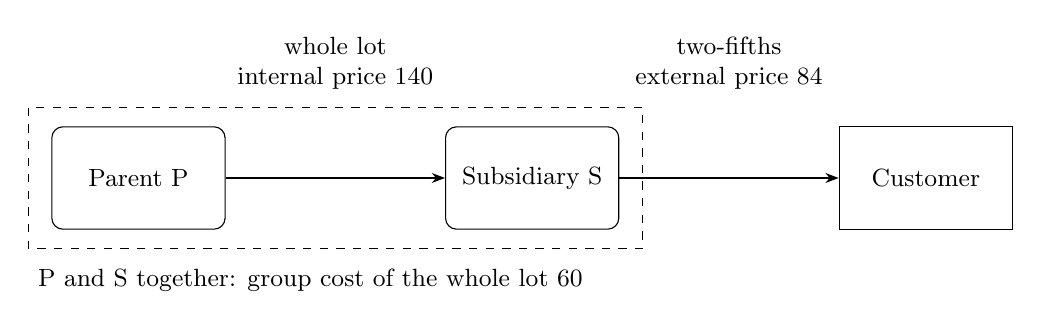
\begin{tikzpicture}[>=Stealth, every node/.style={font=\small}]
\node[draw,rounded corners,minimum width=22mm,minimum height=13mm] (p) at (0,0) {Parent P};
\node[draw,rounded corners,minimum width=22mm,minimum height=13mm] (s) at (5,0) {Subsidiary S};
\node[draw,minimum width=22mm,minimum height=13mm] (c) at (10,0) {Customer};
\draw[->] (p)--node[above=10mm,align=center]{whole lot\\internal price 140} (s);
\draw[->] (s)--node[above=10mm,align=center]{two-fifths\\external price 84} (c);
\draw[dashed] (-1.4,-0.9) rectangle (6.4,0.9);
\node[anchor=west] at (-1.4,-1.3) {P and S together: group cost of the whole lot 60};
\end{tikzpicture}
\caption{The internal price changes the legal books; the external sale determines group revenue.}
\end{figure}

After the external sale, S carries three-fifths of its purchase price, or 84.
The same physical stock cost the group only \(3(60)/5=36\). Its unrealised
internal profit is therefore \(84-36=48\). IFRS~10.B86(c) requires full
elimination of intragroup amounts and of profit still contained in assets; it
also directs the resulting temporary differences to IAS~12.

For clarity, let \(T\) be the internal price, \(C\) the group's original cost
and \(s\) the fraction sold externally. The remaining internal profit is
\begin{equation}
 U=(T-C)(1-s)=(140-60)(1-2/5)=48.
 \label{eq:joined-unrealised}
\end{equation}
The group removes internal revenue 140 and reduces the combined legal cost of
sales by \(T-U=92\). S's tax base remains 84, while group carrying amount is
36. The deductible difference 48 gives a deferred tax asset 12 at the supplied
25\% rate. The after-tax elimination is consequently 36. If all the stock were
sold outside the group, \(s=1\), both the remaining profit and this deferred
tax asset would be zero.

P's first-half pretax profit is \(80-4-10-10=56\). The return timing difference
reduces taxable income to 32, giving current tax 8; deferred tax expense 6
leaves P profit 42. S earns 28 before tax and 21 after current tax 7. Both
current-tax amounts are paid. Group profit is therefore
\begin{equation}
 \Pi_{H1}=42+21-48+12=27.
 \label{eq:joined-h1-profit}
\end{equation}
The downstream margin originated in P's sale. Its after-tax elimination belongs
to P's shareholders; NCI receives 20\% of S's legal profit 21, or 4.2. At June
the group has cash 511, inventory 56, plant 90 and deferred tax asset 12, totalling
669. It has no remaining external liability in this case. Equity is parent
644.8 plus NCI 24.2. These totals reconcile the same shared legal books used by
the return and debt methods.

\subsection{Buying more shares changes who owns the equity}

On 1 July P pays 20 to the outside shareholders for another 10\% of S. P now
owns 90\%, and control is unchanged. In P's separate books, its cost-policy
investment increases by 20 and cash decreases by 20. S records nothing: the
payment was between its shareholders. The group's accounting must instead
describe a change in the relative claims of P's owners and NCI.

Immediately before purchase, S's equity is 121 and NCI owns 20\%, carrying
24.2. P buys half of that interest. The NCI reduction is 12.1, not the cash
price 20. IFRS~10.23 and B96 put the difference directly in parent equity:
\begin{align}
 \Delta NCI&=-(0.90-0.80)121=-12.1,\\
 \Delta E_P&=-(20-12.1)=-7.9.
 \label{eq:joined-nci-purchase}
\end{align}
No gain, goodwill or remeasurement is introduced. IAS~7.42A--42B classifies the
group cash payment as financing, while the parent's separate purchase of an
investment is investing under its own cash-flow presentation
\citep[IFRS~10.23,B96; IAS~7.16,42A--42B; IAS~27.10]{eu20231803}.

The purchase date matters for later earnings. First-half NCI profit remains
4.2; it is not recomputed at 10\%. The new fraction applies to subsequent
profit. Recording only an ending ownership percentage would lose that history
and allocate the year's earnings incorrectly.

\subsection{The external sale releases both margin and tax}

In the second half S sells the remaining lot for 126. Its legal cost is 84,
so legal pretax profit is 42 and tax is 10.5. The group's cost is only 36.
The earlier elimination of 48 now reverses, and the associated deferred tax
asset 12 is consumed. P separately sells its recovered inventory for 40 at
cost 20 and records a further depreciation charge 10. Its second-half pretax
profit is 10 and tax is 2.5. All current taxes are paid.

The resulting group profit is
\begin{equation}
 \Pi_{H2}=(10-2.5)+(42-10.5)+48-12=75.
 \label{eq:joined-h2-profit}
\end{equation}
NCI receives 10\% of S's after-tax profit 31.5, or 3.15. The group release
again belongs to P's shareholders because it reverses P's downstream margin.
Annual NCI profit is \(4.2+3.15=7.35\), and annual parent profit is
\(102-7.35=94.65\). Closing equity can now be reconstructed without using
an asset total as a balancing plug:
\begin{align}
 E_P^{close}&=622+94.65-7.9=708.75,\\
 NCI^{close}&=20+7.35-12.1=15.25.
\end{align}
Their sum is 724, equal to closing cash 644 and plant 80. The inventory has
been sold, the return and debt obligations settled, and the temporary
differences in this case reversed.

The comparison below follows the derivation rather than replacing it. The
balance-sheet columns are closing amounts; income and cash columns are flows
over the stated interval.
\begin{center}
\begin{tabular}{lrrr}
\toprule & First half & Second half & Full year\\\midrule
External revenue &84&166&250\\
Cost of sales &20&56&76\\
Profit before tax &36&100&136\\
Current tax expense &15&13&28\\
Deferred tax expense/(benefit) &-6&12&6\\
Profit after tax &27&75&102\\
NCI share of profit &4.2&3.15&7.35\\
Operating cash flow &1&153&154\\
Financing cash flow &-90&-20&-110\\
Closing cash &511&644&644\\
Closing group equity &669&724&724\\\bottomrule
\end{tabular}
\end{center}

Cash provides an independent check on the joins. External receipts are
\(84+126+40=250\). Operating payments are refunds 40, handling 8, wages 10,
interest 10 and tax 28, totalling 96. Financing payments are debt principal 90
and the NCI purchase 20. Thus
\begin{equation}
 C^{close}=600+(250-96)-(90+20)=644.
\end{equation}
The internal receipt 140 and payment 140 are removed from their respective
gross totals. Merely observing that they net to zero would overstate both
group receipts and payments. Group adjustments never alter either entity's
legal cash ledger.

\subsection{The implementation consequence of a joined close}

Each method receives the current shared state, not its own duplicate cash
balance. The internal sale and settlement each update both legal books as one
transaction; an unmatched invoice or one-sided publication is refused. A
report must link an uninterrupted receipt sequence from its opening state to
its closing state. Consolidation recomputes the required worksheet adjustment
from legal balances and lot history at each date. It does not append the June
elimination again in December.

The companion specification, \code{CompanyComposition/1}, fixes these inputs,
events and outputs in closed records. An independent calculation reconstructs
the legal and group reports, including the adverse cases of balanced but wrong
journals, missing tax findings, changed ownership identities and partial
publication. Its two narrow migration examples preserve the original source
owners and dates; they do not rename a previous synthetic company into P.
Section~\ref{sec:company-composition-reference} gives the exchange details.

This joined case establishes the stated calculation and record design for the
supplied opening. It does not reconstruct the prior acquisition or issuance,
nor does a corporate group with no bank or insurance business specify those
sectors' combined statements. Foreign currency, wider ownership rights, actual
tax authority and the remaining accounting methods retain their own required
evidence. Those limits identify what the next case must add without obscuring
what the shared company close already demonstrates.


\section{Apple: source labels do not identify exposure}
\label{sec:apple}

The real reference package is Apple's 2024 Form 10-K and first-quarter 2025
Form 10-Q, for fiscal dates 28 September and 28 December 2024 respectively
\citep{apple2024,apple2025q1}. The annual balance sheet also supplies
30 September 2023. The annual filing is archived as the company's PDF from
AnnualReports; the interim filing is archived from SEC EDGAR with its inline
XBRL. Apple's Note 1 describes a 52/53-week year ending on the last Saturday
of September. Calendar-year assumptions would therefore misstate the periods.

The package inventory preserves every annual PDF page and every interim
top-level section, all thirteen annual notes and all ten interim notes.
It records internal cross-references and externally incorporated material,
including the proxy statement, as distinct obligations. Statement and debt
facts below are structured; policies, other notes and exhibits retain their
source locations and specific modelling obligations. This is complete
inventory coverage of the acquired files, with partial semantic formalisation.
It does not claim to reconstruct every Apple contract or to have acquired
every incorporated external document.

Apple's annual balance sheet reports assets 364,980, liabilities 308,030 and
equity 56,950, in millions of US dollars. Note 9 reports term-debt principal
97,341, unamortised discount/premium and issuance costs of $-321$, and hedge
accounting adjustments of $-358$. Thus its carrying amount is
$97{,}341-321-358=96{,}662$, split into current 10,912 and non-current
85,750. Fair value is separately disclosed as 88.4 billion. None of these
three measurements may replace another merely because a table calls it debt.

Note 9 identifies the notes as fixed-rate, then states that interest-rate
swaps effectively convert a portion to floating rates. Note 4 reports
interest-rate contract notional of 14,575 at the annual date. A notional is
neither a liability carrying amount nor sufficient information for an exact
interest sensitivity: reset timing, remaining periods, curve conventions and
hedge coverage still matter. The cross-reference connects the derivative to
the borrowing without erasing either contract.

At the interim date, total term-debt carrying amount is
$10{,}848+83{,}956=94{,}804$. Cash is 30,299, total assets 344,085,
liabilities 277,327 and equity 66,758. The interim debt note's rounded
``94.8 billion'' and the statement's 94,804 million can coexist; their
precision differs. Treating them as conflicting exact numbers would create
an artificial infeasibility.

These balances leave two practical financing questions open: how much cash can
fund a payment, and when the payment falls due. The annual cash and cash
equivalents balance of 29,943 includes 2.6 billion held in escrow and restricted
from general use for the State Aid tax obligation. Note 4 states the inclusion
explicitly, and Note 7 connects the escrow to that obligation
\citep[Notes 4 and 7, printed pp.~37 and 39]{apple2024}. Subtracting the reported
restricted component gives $29{,}943-2{,}600=27{,}343$ million as an indicative
remainder at the displayed amounts. The restricted component is rounded to
tenths of a billion, so this subtraction does not establish an exact freely
available balance. The earlier case annotation that described the reported
cash balance as excluding restricted cash was wrong relative to this footnote.
Correcting that interpretation changes funding calculations without changing
the issuer's reported number. It also requires revisiting any liquidity result
that relied on the exclusion.

The debt movement supplies a second reason to preserve a calculation's missing
terms. The first-quarter cash flow statement reports repayments of term debt of
1,009 million, while carrying amount falls by
$96{,}662-94{,}804=1{,}858$ million. At the displayed amounts, the reconciliation is
\[
       94{,}804=96{,}662-1{,}009-849.
\]
The 849 million is the residual after the reported cash repayment; it does not
identify an exchange loss, an income-statement charge or a particular journal.
Explaining it requires the missing movement information, including applicable
currency, discount/premium and hedge-accounting effects. The quarterly cash
flow statement still reconciles independently: operating inflow 29,935 plus
investing inflow 9,792 less financing outflow 39,371 gives the reported cash
increase of 356, from 29,943 to 30,299 million
\citep[statement of cash flows and Note 6]{apple2025q1}. A balanced cash bridge
therefore does not identify the debt history.

The annual filing's securities exhibit adds terms that a debt-total query
cannot supply. Exhibit 4.1 describes two euro-denominated series bearing the
year 2025 in their names. Its reported outstanding principal is dated
18 October 2024, after the annual balance-sheet date. The description concerns
Apple Inc. as issuer, rather than every subsidiary in the consolidated group
\citep[Exhibit 4.1, pp.~3--4]{apple2024}.

\begin{center}
\begin{tabular}{lrrl}
\toprule
Series & Principal (EUR m) & Fiscal year & Scheduled maturity\\\midrule
0.875\% 2025 Notes &1,250&2025&24 May 2025\\
0.000\% 2025 Notes &1,000&2026&15 November 2025\\\bottomrule
\end{tabular}
\end{center}

Apple's disclosed 52-week fiscal 2025 ends on 27 September 2025 under its
last-Saturday convention. The November maturity therefore belongs to fiscal
2026 even though the bond's name says 2025. The annual Note 9 principal-payment
schedule uses fiscal years, whereas the instrument's stated maturity is a
calendar date. Joining those fields on their year number would put a billion
euros of scheduled principal into the wrong fiscal bucket. Neither the later
holding date nor the euro principal may be silently substituted for a
September US-dollar consolidated balance.

Suppose the disclosed faces remain outstanding until scheduled maturity, with
no early redemption, default or additional withholding-related payment, and
euro remains the payment currency. The annual coupon on the 0.875\% series is
then the reported face multiplied by the stated rate:
\[
       1{,}250\times0.00875=10.9375\quad\text{million EUR}.
\]
Its final scheduled principal plus annual coupon is consequently
1,260.9375 million EUR; the zero-coupon series has 1,000 million EUR of
scheduled principal and zero stated coupon. Both scheduled maturity dates
fall on a Saturday. Exact settlement requires the applicable payment-adjustment
provision and business calendar. Exhibit 4.1 is expressly a summary qualified
by the 2013 and 2018 indentures; its payment-currency exceptions and redemption
rights also matter. The retained 2021 indenture cannot replace those earlier
contracts. The calculation establishes conditional scheduled amounts, while
their exact settlement dates and subsequent holdings remain unresolved.

Those missing facts have different consequences for the financial statements.
Principal and coupon payments reduce cash, but settling principal differs from
recognising interest expense. The latter also depends on carrying amount,
effective-interest accrual and the treatment of discounts and hedges; Note 9
expressly includes applicable amortisation and hedging adjustments in effective
rates. Exchange rates, hedge designations and tax treatment can affect profit,
other comprehensive income, retained earnings and closing debt differently.
The cash flow statement additionally needs the payment classification and any
associated hedge settlements. A usable answer thus carries the conditional
euro schedule together with these unresolved dependencies. A dollar company
forecast must supply consistent holdings, exchange, hedge and tax assumptions
across all affected statements.

To demonstrate a source-to-forecast calculation, freeze the interim balance
sheet and apply a \emph{marginal} financing stress for a following 13-week
period: a 200-basis-point rate increase, no principal change, no offsetting
hedge beyond the explicitly selected exposure, immediate cash settlement and
no tax effect. An assumed effective floating exposure $E=14{,}575$ million
produces $0.02\times(13/52)E=72.875$ million additional interest. This exposure
uses the annual notional as a conditional input; it is not asserted to be the
interim net sensitivity. Under that condition, debit interest expense and
credit cash by 72.875. The resulting marginal statements have cash 30,226.125,
assets 344,012.125, liabilities 277,327, equity 66,685.125, profit and comprehensive
income of $-72.875$, and operating cash flow of $-72.875$ relative to the frozen
baseline. The balance-sheet difference equals the equity difference exactly.

If exposure is instead only restricted to $0\leq E\leq14{,}575$, the
conditional added interest lies in $[0,72.875]$ before monetary rounding. That
restriction is a stress assumption and is not claimed to bound every real
Apple exposure. This real case verifies evidence, context, mappings and a
coherent marginal propagation. Northstar supplies the complete-company
forecast; a complete Apple forecast remains dependent on its unmodelled
operations and undisclosed terms.

\section{Apple: five statements constrain one year}
\label{sec:apple-statements}

The debt example leaves a larger question: can the reported profit, changes
in equity and cash flows describe the same financial year? Apple's five
consolidated statements supply a useful starting point. Their fiscal 2024
amounts refer to the year ending 28 September 2024; the opening balance sheet
is dated 30 September 2023. All monetary amounts below are millions of US
dollars. The operations statement's per-share amounts and weighted share
counts keep their separate units \citep[printed pp.~29--33]{apple2024}.

Products revenue of 294,866 and services revenue of 96,169 sum to 391,035.
Their costs, 185,233 and 25,119, leave gross margin of 180,683. Research and
development of 31,370 and selling, general and administrative expense of
26,097 reduce that amount to operating income of 123,216. Other income of
269 and an income-tax provision of 29,749 give net income of 93,736
\citep[printed p.~29]{apple2024}. This same net income enters both the equity
statement and the operating-cash reconciliation. It is one period result
appearing in three statements, so it must not be added three times.

Other comprehensive income supplies the next connection. Foreign-currency
translation contributes 395 after tax. Derivative fair-value changes of
$-832$ and reclassification adjustments of $-1{,}337$ contribute $-2{,}169$;
marketable-debt fair-value changes of 5,850 and reclassifications of 204
contribute 6,054. Thus OCI is $395-2{,}169+6{,}054=4{,}280$, and total
comprehensive income is $93{,}736+4{,}280=98{,}016$
\citep[printed p.~30]{apple2024}. Adding the period OCI to opening accumulated
other comprehensive loss of $-11{,}452$ gives the closing $-7{,}172$.
That accumulated balance, rather than the period flow, enters the balance
sheet.

Despite positive comprehensive income, total equity falls. The equity
statement explains the difference: common-stock issuance adds 1,423 and
share-based compensation adds 12,034; withholding reduces the capital
component by 3,993 and retained earnings by 1,612; declarations reduce
retained earnings by 15,218 and repurchases by 95,846
\citep[printed p.~32]{apple2024}. These movements, apart from comprehensive
income, total $-103{,}212$. The complete equity reconciliation is therefore
\[
62{,}146+98{,}016+1{,}423+12{,}034-3{,}993-1{,}612
 -15{,}218-95{,}846=56{,}950.
\]
The components reconcile separately: capital rises from 73,812 to 83,276,
the accumulated deficit moves from $-214$ to $-19{,}154$, and accumulated
other comprehensive loss moves from $-11{,}452$ to $-7{,}172$. These are
the three closing equity components reported on the balance sheet. Their
agreement prevents a model from explaining the correct total with the wrong
allocation among capital, retained earnings and accumulated OCI.

The same change appears in net assets. Table~\ref{tab:apple-statement-join}
compares the reported endpoints; its changes are derived subtractions
\citep[printed p.~31]{apple2024}. Assets rise by 12,397 while liabilities
rise by 17,593, leaving a 5,196 decrease in equity, exactly the decrease
from the equity reconciliation.

\begin{table}[htbp]
\centering
\begin{tabular}{lrrr}
\toprule &30 September 2023&28 September 2024&Change\\\midrule
Assets&352,583&364,980&12,397\\
Liabilities&290,437&308,030&17,593\\
Equity&62,146&56,950&$-5{,}196$\\\bottomrule
\end{tabular}
\caption{The balance-sheet change agrees with the complete equity movement.
The agreement constrains a history without identifying its transactions.}
\label{tab:apple-statement-join}
\end{table}

Cash follows a different reconciliation. Starting from the same net income,
the cash-flow statement adds depreciation and amortisation of 11,445,
share-based compensation expense of 11,688 and other adjustments of
$-2{,}266$. These three adjustments sum to 20,867. Its six operating-asset
and liability adjustments are net receivables $-3{,}788$, vendor non-trade
receivables $-1{,}356$, inventory $-1{,}046$, other assets $-11{,}731$,
payables $+6{,}020$ and other liabilities $+15{,}552$. They sum to 3,651,
giving operating cash of $93{,}736+20{,}867+3{,}651=118{,}254$
\citep[printed p.~33]{apple2024}. The full indirect bridge is thus present;
none of its broad adjustment rows has been replaced by a presumed change in
a similarly named balance-sheet account.

Investing cash is also positive: security purchases of $-48{,}656$,
maturities of 51,211, sales of 11,135, plant-acquisition payments of
$-9{,}447$ and other investing cash of $-1{,}308$ sum to 2,935. Financing
uses 121,983: employee-award tax payments of 5,441, dividend payments of
15,234, share repurchases of 94,949, debt repayments of 9,958 and other
outflows of 361 outweigh net commercial-paper proceeds of 3,960. The source
shows a dash for net term-debt issuance; the displayed total treats that row
as making no contribution, while the source reading retains the dash.
The three activity totals give
\[
118{,}254+2{,}935-121{,}983=-794,
\qquad 30{,}737-794=29{,}943.
\]
The opening and closing amounts here are cash, cash equivalents and restricted
cash and cash equivalents, as defined by the cash-flow statement. Opening
balance-sheet cash is only 29,965, so the cash-flow population exceeds it by
772; both closing amounts are 29,943. Consequently, the balance-sheet line
falls by 22 while the cash-flow total falls by 794. The earlier 772 remains
unallocated in the retained evidence. It cannot be relabelled as the closing
2.6 billion escrow, which Note 4 explicitly includes in reported cash and
equivalents \citep[printed p.~33 and Note 4, printed p.~37]{apple2024}.

These joins expose the missing transaction links more precisely. Annual
receivables rise by 3,902, leaving 114 after adding their $-3{,}788$ indirect
adjustment. Inventory rises by 955, leaving $-91$ after its $-1{,}046$
adjustment. Payables rise by 6,349, exceeding their 6,020 adjustment by 329.
Even the exact opposite vendor-receivable movements identify neither gross
purchases nor collections. The notes examined below must supply the relevant
recognition, valuation, currency and settlement information; the residuals
themselves supply no such explanation.

Nor can the equity rows simply replace financing cash flows. The reported
repurchase reduction of 95,846 exceeds cash repurchases of 94,949 by 897;
withholding reductions total 5,605 against cash tax payments of 5,441; and
equity compensation of 12,034 differs from the 11,688 expense adjustment.
Cash dividends of 15,234 exceed declarations of 15,218 by 16. Those
differences remain unassigned to particular settlements, fees, taxes or
recognition periods \citep[printed pp.~32--33]{apple2024}. The later note
examples retain their own evidence and conditional histories.

A reconstruction must now satisfy the statement relationships together.
Correct total cash cannot excuse wrong equity components, and correct net
assets cannot excuse omitted cash-flow adjustments. The five statements
constrain a common history, but their agreement does not reveal all gross
events, dates, counterparties or accounting treatments. Those unresolved
links determine which historical alternatives can be supported and what
additional facts a conditional future path still needs.

\subsection{The following quarter must start from the same balances}

The next filing makes the time connection testable. Its balance-sheet
comparison is 28 September 2024, and all 27 monetary rows reproduce the
annual closing column. Its income, comprehensive-income, equity and cash-flow
comparisons instead cover the three months ending 30 December 2023. Those
earlier-quarter flows cannot become the opening amounts for the quarter ending
28 December 2024. The interim statements are explicitly unaudited
\citep[printed pp.~1--5]{apple2025q1}.

Quarterly products revenue of 97,960 and services revenue of 26,340 total
124,300. Cost of sales of 66,025 and operating expenses of 15,443 leave
operating income of 42,832; other expense of 248 and tax expense of 6,254
give net income of 36,330. Translation OCI of $-625$, derivative OCI of
2,435 and marketable-debt OCI of $-1{,}427$ add 383, giving comprehensive
income of 36,713 \citep[printed pp.~1--2]{apple2025q1}. The resulting
equity movement begins at the same 56,950 that closed the annual record.
Compensation adds 3,383, withholding removes 1,891 from capital and 1,102
from retained earnings, declarations remove 3,819 and repurchases remove
23,476. Together these other movements are $-26{,}905$, so
$56{,}950+36{,}713-26{,}905=66{,}758$. Capital, accumulated deficit and
accumulated OCI also join separately at both endpoints
\citep[printed pp.~3--4]{apple2025q1}.

Assets decline by 20,895 to 344,085 and liabilities decline by 30,703 to
277,327. Their difference gives the same 9,808 equity increase. This check
connects the period result to the balance sheet without confusing declining
assets with a loss. The retained earnings deficit improves by 7,933, capital
rises by 1,492 and accumulated OCI rises by 383; these three changes also
sum to 9,808.

The cash reconciliation supplies a different account of the quarter.
Depreciation and amortisation of 3,080, compensation expense of 3,286 and
other adjustments of $-2{,}009$ add 4,357 to net income. The six operating
asset/liability adjustments are $+3{,}597$, $+3{,}166$, $+215$, $+939$,
$-6{,}671$ and $-11{,}998$, in the same reported categories used for the
annual reconciliation. They total $-10{,}752$, so operating cash is
$36{,}330+4{,}357-10{,}752=29{,}935$. Investing cash adds 9,792 and
financing uses 39,371, leaving a 356 increase from 29,943 to 30,299
\citep[printed p.~5]{apple2025q1}. Both cash-flow endpoints now match the
corresponding balance-sheet amounts. That numeric match still does not make
every dollar unrestricted.

Adjacent flows may now be combined for a deliberately longer question.
Over fiscal 2024 and the following quarter together, comprehensive income is
134,729 and the other equity movements total $-130{,}117$. Over that same
interval, operating, investing and financing cash total 148,189, 12,727 and
$-161{,}354$. The two cumulative reconciliations are
\[
62{,}146+134{,}729-130{,}117=66{,}758,
\qquad
30{,}737+148{,}189+12{,}727-161{,}354=30{,}299.
\]
These are derived amounts for the interval from 1 October 2023 through
28 December 2024, not an issuer annual statement or a trailing-twelve-month
result. Endpoint balances are carried forward, not added. EPS and weighted
share averages also cannot be summed as if they were dollar flows.

The quarter preserves several distinctions that a common schema might
otherwise erase. The annual equity table contains a common-stock issuance
row and the annual cash-flow table contains a term-debt issuance row; the
interim tables omit both. The interim reported totals reconcile over their
own disclosed rows. A comparison record may describe those omissions, but
must not manufacture two issuer-reported zeros. The prior-year quarter's
term-debt repayment dash is likewise retained in its own dated column
\citep[printed pp.~4--5]{apple2025q1}.

Transaction uncertainty remains across the joined interval. In the current
quarter, the receivable change plus its indirect adjustment leaves $-174$;
inventory leaves $-160$. The payable change is $-7{,}050$, differing from
the $-6{,}671$ adjustment by $-379$. Cash dividends exceed declarations by
37, and cash repurchases exceed the equity reduction by 130. None identifies
the missing settlement, valuation or timing components. The subsequent note
inquiries must retain these relationships together when testing historical
alternatives. Combining individually compatible note examples does not by
itself establish that they share a compatible cash, income and equity history.


\section{Apple: revenue recognition and cash collection}
\label{sec:apple-revenue}

An iPhone sale can create revenue today and an obligation to provide services
later. Apple's annual revenue note separates delivered hardware and bundled
software from the right to receive product-related services such as iCloud,
Siri and Maps. It allocates the price and related discounts by relative
stand-alone selling prices. For the bundled services those prices are estimates,
because observable separate prices are unavailable. The hardware portion is
recognised when control transfers, generally on shipment; the service portion
is deferred and recognised straight-line over the estimated period of provision
\citep[Note 2, printed p.~35]{apple2024}. A historical model consequently needs
the allocation and service cohort as well as the sale date and amount. Neither
the product label nor the customer payment supplies those missing terms.

The note describes collection shortly after control transfer or the start of
service delivery. It does not specify one collection lag for every contract.
Products revenue also reflects expected returns, price protection and customer
incentives. Revenue excludes taxes collected for remittance to governments
\citep[Notes 1--2, printed pp.~34--35]{apple2024}. Together these qualifications
prevent a simple conversion of reported revenue into gross customer receipts.

Presentation creates a second distinction. Where Apple obtains control of a
third-party product before sale, it reports the gross amount billed. For
third-party applications sold through the App Store, its stated treatment
records only the retained commission in Services revenue. Services also already
includes recognition of the deferred value of services bundled with products
\citep[Note 2, printed p.~35]{apple2024}. Adding that recognition to reported
Services a second time would double count it; treating Services as gross App
Store customer spending would change the measured quantity.

The product and geographic tables describe different divisions of the same
sales. The five product/service rows sum to 391,035 million dollars in fiscal
2024 and 124,300 million in the quarter ended 28 December 2024. The geographic
segment sales sum to those same totals. They must not be added together.
Apple says the product mix is generally similar across segments, except that
iPhone represents a moderately higher share in Greater China. That qualitative
statement does not identify a product-by-region matrix
\citep[Notes 2 and 13, printed pp.~35--36 and 46--47]{apple2024}
\citep[Notes 2 and 10, printed pp.~6 and 11]{apple2025q1}.

\subsection{The movement that the note leaves unidentified}

At 28 September 2024 Apple reports total deferred revenue of 12.8 billion
dollars. At 28 December it reports 13.2 billion, and says that quarter's net
sales include 3.7 billion recognised from the deferred balance at the September
date \citep[Note 2, printed p.~6]{apple2025q1}. The balance sheet's December
current deferred-revenue line is 8,461 million, with 8,249 million at September
\citep[printed p.~3]{apple2025q1}. Those are current liabilities; the note's
larger amounts are totals. The precision differs too: the total is displayed
to tenths of a billion, whereas the current line is displayed in millions.

Let $D_0$ and $D_1$ denote opening and closing total deferred revenue. During
the quarter, let $A$ be additions to deferred revenue, $R_o$ revenue released
from the opening balance, and $R_n$ revenue released from amounts added during
the quarter. Let $M$ collect other signed movements, positive when they increase
the liability. These symbols describe a balance reconciliation; $M$ is not an
assertion that a particular adjustment occurred. In billions of dollars,
\begin{equation}
 D_1=D_0+A-R_o-R_n+M,
 \qquad A-R_n+M=D_1-D_0+R_o\simeq13.2-12.8+3.7=4.1.
 \label{eq:apple-deferred-movement}
\end{equation}
The source identifies $R_o$, not the whole release $R_o+R_n$. The 4.1 billion
residual therefore measures net additions after new-origin releases and other
movements at the displayed amounts. Calling it gross new deferrals, billings
or cash collected would be wrong relative to what has been calculated.

Rounding also matters. If each of the three displayed inputs is rounded to the
nearest 0.1 billion, a closed outer envelope for that residual is
$[3.95,4.25]$ billion: the lower endpoint uses $13.15-12.85+3.65$, and the
upper uses $13.25-12.75+3.75$. This is a conditional precision calculation,
not a verified issuer rounding rule or a bound on gross collections. Its
endpoints leave the treatment of exact rounding ties unspecified.

Two constructed histories make the missing movement visible. For this
illustration alone, use the displayed amounts as exact inputs and set $M=0$.
Keep the reported quarter's total revenue at 124.3 billion. The table supplies
two different choices for $A$ and $R_n$; other recognised revenue is the
remainder needed to match that total.

\begin{center}
\begin{tabularx}{\linewidth}{@{}Xrr@{}}
\toprule
Quarterly amount (USD billion) & History 1 & History 2\\\midrule
New deferrals, $A$ & 4.1 & 5.1\\
Release from those new deferrals, $R_n$ & 0 & 1.0\\
Release from the opening balance, $R_o$ & 3.7 & 3.7\\
Other recognised revenue & 120.6 & 119.6\\
Closing deferred revenue & 13.2 & 13.2\\
Total recognised revenue & 124.3 & 124.3\\\bottomrule
\end{tabularx}
\end{center}

Both histories satisfy the selected note totals, yet their new deferrals differ
by one billion. They are witnesses within this aggregate model, not reconstructed
Apple contracts or a fit to every financial-statement constraint. Additional
contract, cohort, return and movement information can rule out or refine them.
No probability attaches to either merely because two examples were written down.

The corresponding recognition entry debits deferred revenue and credits revenue
when service is provided. Receipt or billing of consideration that creates the
deferral instead credits deferred revenue and debits cash or, where an
unconditional right to payment exists, a receivable. Collection of that
receivable changes cash and receivables without creating revenue a second time.
For example, hold History 1's other revenue cash-settled and omit costs, taxes,
refunds and other movements solely to isolate this subsystem. Receiving its
4.1 billion of new consideration gives revenue-side cash inflow 124.7 billion.
If that new consideration is receivable at quarter end, cash inflow is 120.6
billion and receivables increase 4.1 billion. In both cases the asset increase
is 124.7, matched by a 0.4 increase in deferred revenue and 124.3 of revenue
before omitted expenses. These conditional entries explain the identification
problem; neither inflow is an estimate of Apple's actual cash collections.

\subsection{A dated recognition expectation is not a cash forecast}

At both September and December, Apple expects 64\% of the then-reported total
deferred revenue to be realised in less than a year, 25\% within one to two
years, 9\% within two to three years and 2\% after three years
\citep[Note 2, printed p.~36]{apple2024}
\citep[Note 2, printed p.~6]{apple2025q1}. These are two dated expectations
about two balances. Multiplication at the displayed December values gives
$13.2\times0.64=8.448$ billion in the first bucket. The corresponding September
calculation gives 8.192 billion. Their difference does not measure revenue
recognised during the intervening quarter: the dates, remaining horizons and
contract populations have changed.

The percentages divide an expected amount by recognition horizon. They do not
assign probabilities to alternative histories, fix collection dates or forecast
all future sales. The 8.448 billion calculation also cannot replace the reported
8.461 billion current liability. Rounded amount and percentage disclosures do
not justify an exact equality between those figures, and the query must retain
the source's distinct description of each quantity. A future calculation that
requires monthly service or receipts needs finer timing and payment evidence.

The note leaves another part of future service unquantified. For certain
long-term arrangements, Apple has not yet delivered the service, has no right
to bill for it and attributes the unbilled consideration entirely to that
undelivered service. It reports neither revenue nor an amount for those
obligations in this passage \citep[Note 2, printed p.~35]{apple2024}. A query
must retain an unknown amount; setting it to zero or equating it with recorded
deferred revenue would erase the distinction the company makes.

These disclosures therefore yield several different results. The total and
current deferred balances are reported observations. The 4.1 residual is a
derived net movement with unresolved components. The recognition buckets are
management's dated expectations, and the excluded consideration is unquantified.
Contract-level allocations, service lives, new-origin releases and collection
facts remain necessary for a particular future journal path. The annual and
interim periods also stay separate: the December 2024 quarter follows the
September 2024 fiscal year, so subtracting it from that annual revenue cannot
produce the year's final nine months. The complete revenue-note reading makes
these consequences explicit while the wider Apple disclosure package remains
only partly formalised.

\section{Apple: commitments and the cash needed to fulfil them}
\label{sec:apple-commitments}

The same distinction between recognition and cash arises when Apple buys
capacity and components. A lease liability measures one part of an existing
obligation; a purchase commitment describes goods or services still to be
acquired. A funding projection needs the payments arising from both, together
with new orders and operating decisions. Adding every disclosed amount would
mix measurements and could count the same requirement twice.

\subsection{From a lease liability to future payments}

At 28 September 2024, Apple's lease note reports the following amounts in
millions of dollars \citep[Note 8, printed p.~42]{apple2024}. The maturity table
first totals undiscounted payments and then deducts imputed interest to reach
the recognised liability. The right-of-use assets are reported separately.

\begin{center}
\begin{tabularx}{\linewidth}{@{}Xrrr@{}}
\toprule
Amount (USD million) & Operating & Finance & Total\\\midrule
Undiscounted lease payments & 13,518 & 1,272 & 14,790\\
Less: imputed interest & 1,984 & 376 & 2,360\\
Recognised lease liabilities & 11,534 & 896 & 12,430\\
Right-of-use assets & 10,234 & 1,069 & 11,303\\\bottomrule
\end{tabularx}
\end{center}

Thus $14{,}790-2{,}360=12{,}430$ reconciles the maturity and liability
measurements. The recognised liability is already included in the balance
sheet; it is not an extra cash requirement to add to 14,790. Its current
components total $1{,}488+144=1{,}632$ million, whereas the fiscal-2025 maturity
bucket is 1,991 million. A current carrying amount and a gross payment bucket
answer different questions. The right-of-use asset likewise need not equal the
remaining liability; these reported balances do not disclose the complete
amortisation, prepayment and modification history.

Apple also reports 849 million of fixed payments under additional leases that
had not commenced. It expects them to commence in 2025--2026, with terms from
less than one year to twenty-one years. Adding this separately disclosed amount
to the maturity total gives $14{,}790+849=15{,}639$ million. That sum is
consistent, under a nearest-0.1-billion rounding assumption, with the 15.6
billion of fixed lease obligations in management's cash-requirements discussion
\citep[printed pp.~25 and 42]{apple2024}. Numerical compatibility does not
establish a contract-by-contract reconciliation. It neither adds 849 to the
recognised liability nor identifies its commencement and payment dates.

The remaining lease information cannot supply those dates mechanically. The
note describes original terms typically no longer than ten years, with renewal
options, some reasonably certain to be exercised. Its weighted-average
remaining term of 10.3 years describes a different quantity. The reported
3.1\% discount rate, generally based on estimated incremental borrowing rates,
does not supply every contract's rate or the timing hidden in ``thereafter''.
Applying that one rate to invented year-end payments would introduce new
assumptions. The policy combining lease and nonlease components also has a
stated scope: corporate, data-centre and retail facilities
\citep[Notes 1 and 8, printed pp.~34 and 42]{apple2024}.

Fixed and variable costs add another distinction. For 2024, Apple reports
2.0 billion of fixed operating-lease cost, 1.9 billion of fixed operating-lease
cash payments and 1.0 billion of noncash right-of-use assets obtained for lease
liabilities. Variable costs across its leases were 13.8 billion; payments of
that kind primarily depend on purchases of output from the leased assets
\citep[Note 8, printed p.~42]{apple2024}. Historical expense is therefore not a
fixed future cash schedule. Forecasting it requires output, price and settlement
assumptions. Adding it to manufacturing commitments without identifying their
relationship could double count procurement requirements.

\subsection{Why a fall in commitments does not identify cash spent}

The purchase note and management discussion disclose different views. Note 12
lists 11,226 million of future payments under unconditional purchase obligations
whose remaining terms exceed one year. Its fiscal-2025 row is 3,206 million
\citep[Note 12, printed p.~45]{apple2024}. The term restriction selects
contracts; it does not place every payment beyond the coming year. The note
describes these as off-balance-sheet commitments, primarily involving supplier
arrangements, intellectual property, content and distribution rights.

Management's discussion provides additional near-term evidence. At the same
September date it reports manufacturing purchase obligations of 53.0 billion,
of which 52.9 billion is payable within twelve months. Other purchase
obligations total 12.0 billion, with 4.1 billion within twelve months; that
description includes capital assets as well as supplier, content and rights
arrangements \citep[printed p.~25]{apple2024}. A model confined to Note 12
would miss those reported aggregates. Conversely, subtracting 11.226 from 12.0
and labelling the difference short-term contracts is unsupported: the category
and term populations have not been reconciled, and the precision differs.

At 28 December 2024 manufacturing obligations are 39.8 billion, all payable
within twelve months. The interim report says contractual cash requirements
have not changed materially since the annual filing except for commercial
paper, manufacturing obligations and the State Aid tax payable
\citep[printed p.~16]{apple2025q1}. That qualitative statement is not an exact
December lease measurement or evidence that every lease remained unchanged.
The two manufacturing totals are dated observations over changing orders and
payment horizons. Their 13.2 billion difference does not identify purchases
or cash paid during the quarter.

To see what is missing, consider an explicitly simplified model in billions
of dollars. Let $O_0$ and $O_1$ denote a comparable population of undelivered
fixed-price orders at the two dates. Let $N$ be new orders and $F$ the value
removed when goods are delivered. Assume no cancellation, price or currency
change. Treat the displayed 53.0 and 39.8 as exact inputs for this illustration.
These assumptions define the example; the disclosure does not establish this
roll-forward convention for every reported obligation. The balance relation is
\begin{equation}
 O_1=O_0+N-F,\qquad F-N=53.0-39.8=13.2.
 \label{eq:apple-commitment-movement}
\end{equation}
With no new orders, delivery is 13.2. With 5.0 of new orders, delivery is 18.2.
Both leave the same closing undelivered amount of 39.8. The source balances
alone cannot choose between these conditional movements; actual contract
changes and delivery evidence could do so.

Payment is a further choice. Suppose the first history's 13.2 of delivered
goods all remain unsold inventory, with no opening payables, prepayments or tax.
Paying on delivery debits inventory and credits cash by 13.2: total assets and
profit do not change within this subsystem. Delivery on credit instead debits
inventory and credits trade payables by 13.2: assets and liabilities rise
together, with no immediate cash or profit effect. Settling that payable later
debits the payable and credits cash; consumption, sale or impairment would
require further entries. These examples isolate recognition and settlement.
They are not estimates of Apple's actual purchases or payments, or a fit to
all its financial statements. No probability follows from writing two histories.

Delivery assumptions also need the narrative that surrounds the purchase
table. Apple describes single or limited sources for some components,
industry-wide shortages and price fluctuations, and capacity or yield
constraints for new technologies. Suppliers may favour common components over
custom ones. Its named manufacturing locations describe outsourced production,
not a product-by-revenue-region allocation or ownership map
\citep[Note 12, printed p.~46]{apple2024}. A scenario in which input availability
changes may alter output, variable lease payments, inventory and receipts
together. The passage motivates those dependencies without identifying their
size or probabilities.

The same note, and the interim contingency note, preserve management's dated
assessment of unresolved legal claims. At each date, management states that
there was not at least a reasonable possibility that Apple had incurred a
material loss, or a material loss greater than a recorded accrual
\citep[Note 12, printed p.~46]{apple2024}
\citep[Note 9, printed p.~11]{apple2025q1}. It does not make litigation exposure
zero. Contract terms, supply constraints, commencement, delivery and settlement
must therefore remain in the historical record alongside reported balances.
They determine which future journal paths can be supported when a funding
question is asked.

\section{Apple: resources available for payment}
\label{sec:apple-liquidity}

The procurement and settlement choices just described determine when Apple
needs money. Funding those payments requires a second account: what resources
can be used, how securities become cash, and when customers pay. Annual and
interim Note 4 distinguish these questions even though a single total might
appear to answer them. The following table combines the notes' measurement
and balance-sheet classifications. Amounts are in millions of US dollars at
the displayed precision; the December date is the end of the first fiscal
quarter, not another annual endpoint
\citep[Note 4, printed pp.~36--37]{apple2024}
\citep[Note 4, printed pp.~7--8]{apple2025q1}.

\begin{center}
\begin{tabular}{lrrr}
\toprule
Resource / measurement &30 Sep 2023&28 Sep 2024&28 Dec 2024\\\midrule
Cash and cash equivalents &29,965&29,943&30,299\\
Current marketable securities &31,590&35,228&23,476\\
Non-current marketable securities &100,544&91,479&87,593\\\midrule
Total fair value &162,099&156,650&141,368\\
Total adjusted cost &173,752&160,600&147,088\\
Net unrealised gains / losses &$-11,653$&$-3,950$&$-5,720$\\\bottomrule
\end{tabular}
\end{center}

Cash plus the two securities rows equals total fair value. Adjusted cost plus
net unrealised gains and losses provides a second reconciliation of that same
total; it is not an additional resource to add to it. The source calls the
column \emph{adjusted cost}. Relabelling every investment as amortised-cost
debt would erase the different instruments represented in the table.

\subsection{Restriction changes what can be spent}

At September 2024, cash includes 2.6 billion dollars held in escrow, while
marketable securities include a further 13.2 billion. Both are restricted from
general use and designated for the State Aid tax obligation discussed earlier.
Subtracting their displayed centres from the total gives
$156{,}650-2{,}600-13{,}200=140{,}850$ million. MD\&A separately reports
unrestricted cash, equivalents and securities of 140.8 billion
\citep[printed pp.~25--26 and Note 4]{apple2024}. The apparent difference
does not establish conflicting disclosures: the restrictions and the MD\&A
total are rounded to tenths of a billion, whereas the table is in millions.
If each amount is rounded to its nearest displayed quantum, the subtraction
has possible bounds of 140,749.5 and 140,950.5 million. Those bounds overlap
the 140,750 to 140,850 million rounding range for the MD\&A total. This is a
conditional compatibility check, not an issuer-stated rounding convention
or a confidence interval.

The December footnote makes the distinction between maturity and restriction
especially clear: \emph{current} marketable securities include 3.3 billion
dollars of restricted escrow funds, and cash includes 126 million. At the
displayed centres, total resources less this disclosed escrow are
$141{,}368-3{,}300-126=137{,}942$ million. Cash plus current securities is
53,775 million; removing the same escrow gives 50,349 million. These are
indicative subtractions, not exact freely spendable balances. Under the same
nearest-rounding hypothesis the first subtraction ranges from 137,891 to
137,993 million. Interim MD\&A supplies no numerical unrestricted total
\citep[Note 4 and printed p.~16]{apple2025q1}. A current classification
therefore cannot serve as permission to spend an asset, and excluding escrow
does not establish immediate liquidation at the reported price.

Maturity supplies a different kind of timing information. Note 1 tests the
three-month cash-equivalent maturity at \emph{purchase}, while annual Note 4
classifies marketable debt as available-for-sale and assigns current or
non-current status using each instrument's underlying maturity
\citep[printed pp.~34 and 37]{apple2024}. Among non-current debt excluding
mortgage- and asset-backed securities, the September maturity shares are
86\%, 10\% and 4\% for 1--5, 5--10 and more than 10 years. The separate
mortgage- and asset-backed population has shares of 14\%, 9\% and 77\%.
At December these become 85/11/4\% and 13/10/77\%, respectively
\citep[Note 4, printed p.~8]{apple2025q1}. Each triple divides its own
population; the two triples cannot be added. Nor do contractual maturity
bands establish a sale date, sale price or cash receipt schedule. Management's
stated belief in sufficient resources also relies on ongoing operating cash
and continued access to debt markets. It is a dated funding assessment,
rather than a solvency guarantee derived from the table.

\subsection{Security turnover differs from valuation}

Securities can fund payments through sales or maturities, but a fall in their
reported balance need not equal cash released. Fiscal 2024 cash proceeds from
maturities and sales are 51,211 and 11,135 million, while purchases use 48,656.
Net cash released is therefore $51{,}211+11{,}135-48{,}656=13{,}690$ million.
The marketable-security balance falls by only
$126{,}707-132{,}134=-5{,}427$ million
\citep[cash-flow statement, printed p.~33, and Note 4]{apple2024}.
To expose the missing reconciliation, let $M_0$ and $M_1$ be total current
and non-current marketable securities at the period's opening and closing.
Let $C$ be maturity and sale proceeds less purchases, positive when cash is
released. Define $R$ as the unallocated difference between the stock movement
and that cash measure, all in millions over the same period:
\[
\begin{aligned}
 M_1-M_0&=-C+R,\\
 \text{Fiscal 2024:}\quad -5{,}427&=-13{,}690+8{,}263,\\
 \text{First quarter 2025:}\quad -15{,}638&=-13{,}335-2{,}303.
\end{aligned}
\]
For the quarter, the cash measure is
$15{,}967+3{,}492-6{,}124=13{,}335$ million
\citep[cash-flow statement and Note 4]{apple2025q1}. The relation defines a
residual; it does not explain it. Cash sale proceeds differ from the carrying
amount removed on disposal, and changes in measurement or classification may
also enter the stock. Apple's specific-identification policy for securities
sold requires the disposed lots to recover their cost
\citep[Note 1, printed p.~34]{apple2024}. Neither the positive
8,263 nor the negative 2,303 identifies a fair-value, currency or
reclassification journal.

The valuation columns help separate another tempting explanation. Across the
annual dates, total adjusted cost falls by 13,152 million and net unrealised
gains and losses rise by 7,703, producing a total fair-value decline of 5,449.
Across the quarter, the corresponding changes are $-13{,}512$ and
$-1{,}770$, producing $-15{,}282$. These totals include cash and equivalents,
whereas $M_0$ and $M_1$ include only marketable securities. They also differ from the
comprehensive-income statement's net-of-tax marketable-debt amounts: 6,054
million for the year and $-1{,}427$ for the quarter, including reclassification
adjustments \citep[comprehensive-income statement, printed p.~30]{apple2024}
\citep[comprehensive-income statement, printed p.~2]{apple2025q1}. Endpoint
unrealised balances and period OCI differ in population, tax and timing;
their numerical differences cannot be assigned to a tax charge or realised
gain without the missing movements.

Even reported cash needs matching populations. Annual cash-flow cash, cash
equivalents and restricted cash opens at 30,737 million, exceeding opening
balance-sheet cash and equivalents of 29,965 by 772. Both close at 29,943.
Thus the cash-flow change is $-794$, while the balance-sheet line changes by
$-22$; the cause and location of the earlier 772 remain unallocated. The
quarter's endpoint populations agree, giving the same 356 million increase
\citep[balance and cash-flow statements]{apple2024,apple2025q1}.

Valuation risk is likewise distinct from a payment. The notes describe Level 2
prices or models with significant observable inputs and counterparties that
\emph{generally} have high credit ratings. Annual Item 7A reports that a
hypothetical 100-basis-point rate rise at all tenors would reduce investment
fair value, including associated derivatives, by 2,755 million at September
2024 and 3,089 million at September 2023 \citep[printed p.~27]{apple2024}.
Those are dated issuer scenarios, not cash outflows or loss probabilities;
the issuer's valuation model has not been replicated. Interim Item 3's
no-material-change referral does not issue a new December sensitivity.

\subsection{Future receipts need customers and collection dates}

Receivables may turn into cash later, but their movement does not identify
collections. Annual net trade receivables rise by 3,902 million, while the
indirect cash-flow adjustment is $-3{,}788$. Their sum leaves an unallocated
114 million difference. In the quarter, the balance change of $-3{,}771$
and adjustment of $+3{,}597$ leave $-174$. Vendor non-trade changes match
the opposite indirect adjustments exactly: $+1{,}356/-1{,}356$ annually
and $-3{,}166/+3{,}166$ quarterly. Even that match supplies neither gross
sales nor total collections \citep[balance and cash-flow statements]{apple2024,apple2025q1}.
Sales, allowances, currency and noncash movements still need their own
evidence before receipts can be dated.

Concentration describes who might pay, but overlapping descriptions cannot be
summed as separate exposures. Carriers account for 41\%, 38\% and 33\% of
total trade receivables at the three successive dates. At December the note
also identifies two customers individually accounting for at least 10\%, with
shares of 18\% and 11\%. It does not say whether they are carriers
\citep[Note 4, printed p.~38]{apple2024}
\citep[Note 4, printed p.~9]{apple2025q1}. Let $A$ be those two customers,
$B$ the carrier group, and $s(S)$ the share of total trade receivables owed
by customers in a set $S$. Each customer belongs wholly to a set or does not.
Treat the displayed percentages as exact centres for this illustration.
Inclusion-exclusion gives
\[
 s(A\cup B)=s(A)+s(B)-s(A\cap B)
          =29\%+33\%-s(A\cap B).
\]
If both large customers are carriers, their 29\% is already inside the 33\%
carrier share, so the union is 33\%. If neither is a carrier, the union is
62\%. For a concrete construction, allocate receivables across eleven
hypothetical customers with shares
$18,11,9,9,8,7,4,9,9,8,8$ percent. These sum to 100 and only two reach 10\%.
Carriers can be the 18, 11 and 4 customers, totalling 33, or the first
9, 9, 8 and 7 customers, also totalling 33. The same marginal disclosures
therefore permit both endpoint unions. If only one large customer is a carrier,
the union is 44\% or 51\%; exact-centre membership does not permit an
arbitrary continuously divisible overlap. These are conditional percentage
examples, not recovered customer identities or probabilities of loss. The
note's trade denominator is not automatically the balance sheet's \emph{net}
receivable line, so multiplying it by that line would add an unsupported
measurement assumption. Required credit support or collateral applies to
\emph{certain} customers; it does not establish universal recovery.

Vendor non-trade receivables have a separate economic origin and denominator.
Apple buys components from suppliers and sells them to manufacturing vendors
that make subassemblies or final products for Apple. Those component sales
are excluded from product net sales; any gain reduces product cost of sales
when Apple sells the related final products. The two largest reported vendor
shares are 44\% and 23\% at September 2024, and 43\% and 24\% at December,
each pair totalling 67\% on its own dated vendor population
\citep[annual and interim Note 4]{apple2024,apple2025q1}. Equal combined shares
do not establish unchanged counterparties, component cohorts or collection
risk. A funding forecast consequently needs settlements and restrictions on
assets alongside payment dates on obligations. Keeping reported assertions
distinct from those missing facts is the starting point for representing
the company's historical record.

\section{Sales geography is not a map of costs or assets}
\label{sec:apple-segments}

The liquidity question leaves a related operating question. If demand weakens
in one place, which part of Apple's sales and profit is exposed? Apple reports
five geographic segments, but a segment is a management reporting division,
not a list of incorporated companies, factories or product lines. Reading its
two segment notes as though those were the same partitions would make a
regional scenario appear more precise than the filing permits.

\subsection{What the regional labels measure}

Apple's fiscal 2024 Note 13 names Americas, Europe, Greater China, Japan and
Rest of Asia Pacific. Americas covers North and South America. Europe also
includes India, the Middle East and Africa; Greater China includes China
mainland, Hong Kong and Taiwan. Apple says regional net sales are
\emph{generally} based on customer location and sales through retail stores
in those geographic locations. Its segments sell similar products and
services, but are managed separately around customers, distribution partners
and market conditions \citep[Note 13, printed pp.~46--47]{apple2024}. An
India-customer sales shock therefore belongs with Apple's Europe segment
under this disclosure's general attribution rule, even though India is in Asia. Neither this mapping
nor the label ``Greater China'' locates the legal seller, the manufacturing
partner or the cash-receiving entity.

The prior revenue reading established that product and regional net sales are
two classifications of the same 391,035 million dollars in fiscal 2024 and
124,300 million in the first quarter of fiscal 2025; the totals cannot be
added. The full Note 13 and interim Note 10 tables confirm five reported
regional sales and operating-income pairs in each dated column. For example,
Greater China has fiscal 2024 sales of 66,952 million and segment operating
income of 27,082 million; in the quarter ended 28 December 2024 the amounts
are 18,513 and 8,160 million
\citep[Note 13, printed p.~47]{apple2024}
\citep[Note 10, printed p.~11]{apple2025q1}. The quarter is a distinct
three-month period, not a fourth of the fiscal-year observation. Apple's
fiscal calendar can contain 53 weeks, as it did in fiscal 2023, and its
interim MD\&A describes historically higher first-quarter sales associated
in part with the holidays \citep[Note 1 and MD\&A]{apple2024,apple2025q1}.

Management attributes the annual Greater China sales decline mainly to lower
iPhone and iPad sales and reports an unfavourable renminbi effect. For the
first quarter of fiscal 2025 it attributes the decline mainly to iPhone,
while describing a favourable currency effect
\citep[annual and interim segment operating performance]{apple2024,apple2025q1}.
These are dated issuer explanations, not measured contributions of each driver
or an estimated response equation. A future region-specific demand or
exchange-rate path needs product, currency and contract information that the
regional totals alone do not supply.

\subsection{Why segment income cannot be treated as fully allocated profit}

Apple defines each segment's operating income as third-party sales less the
related cost of sales and directly attributable operating expenses. The
annual total of segment operating income is 162,044 million, but the
consolidated operating statement reports 123,216 million. Note 13 supplies
the bridge: 31,370 million of research and development and 7,458 million of
other corporate expenses, net, are subtracted. The latter category includes
general and administrative compensation, various nonrecurring charges and
other separately managed costs. The reported relation is
\begin{equation}
162{,}044-31{,}370-7{,}458=123{,}216
\quad\text{million dollars, fiscal 2024}.
\label{eq:apple-segment-income-bridge}
\end{equation}
The first-quarter fiscal 2025 bridge has the same form:
$53{,}174-8{,}268-2{,}074=42{,}832$ million. Both endpoints agree with the
consolidated statements of operations
\citep[statements of operations and Note 13, printed pp.~29 and 47]{apple2024}
\citep[statement of operations and Note 10, printed pp.~1 and 11]{apple2025q1}.
The annual ``other corporate'' amount is not identical to the 26,097 million
selling, general and administrative expense line in the consolidated
statement. Equating the two would change the reported classification.

Equation~\eqref{eq:apple-segment-income-bridge} identifies the company-wide cost pool, not how it would be
attributed to regions. To see the difference, take a hypothetical allocation
of the 38,828 million total corporate bridge across Americas, Europe, Greater
China, Japan and Rest of Asia Pacific of respectively 14,000, 10,000, 5,000,
4,000 and 5,828 million. Moving 1,000 from Americas to Greater China produces
a second allocation of 13,000, 10,000, 6,000, 4,000 and 5,828 million.
Both are nonnegative, sum to the same corporate total and reproduce the
consolidated 123,216 million. Yet Greater China's hypothetical profit after
these costs is either $27{,}082-5{,}000=22{,}082$ or
$27{,}082-6{,}000=21{,}082$ million. Apple does not report either fully
allocated figure, and the filing supplies no rule preferring one allocation.
These constructions establish numerical nonidentification within the stated
nonnegative illustration; they do not assert that all real cost allocations
are nonnegative or that either construction describes Apple's internal books.
Forecasting regional profit also requires the behaviour of directly
attributable and corporate costs under the scenario.

\subsection{Country sales and long-lived assets answer different questions}

The annual note separately presents country sales for fiscal 2024, 2023 and
2022 and country long-lived-asset stocks at the ends of fiscal 2024 and 2023.
It separately reports countries individually accounting for at least 10\% of
the respective totals and groups the rest; that selection rule does not make
``Other countries'' a single location. The 2024 displayed amounts illustrate
the different populations:
\begin{center}
\begin{tabular}{lrr}
\toprule
Country class & 2024 net sales & Long-lived assets\\
& \multicolumn{2}{c}{USD millions}\\\midrule
U.S. & 142,196 & 35,664\\
China, including Hong Kong and Taiwan & 66,952 & 4,797\\
Other countries & 181,887 & 5,219\\\midrule
Total & 391,035 & 45,680\\\bottomrule
\end{tabular}
\end{center}
The China country-sales row equals Greater China segment sales in all three
annual columns. The note's China footnote includes Hong Kong and Taiwan, so
the equality is a useful check on these displayed populations. It does not
turn that row into a legal-entity or production-location ledger. The U.S.
country-sales row is below Americas segment sales by 24,849 million in 2024;
assigning that difference to particular countries requires the precise
country-to-region attribution and customer facts. Europe's segment label
cannot be substituted for a European-country total because it includes India,
the Middle East and Africa \citep[Note 13, printed pp.~46--47]{apple2024}.

The 45,680 million long-lived-asset total equals net property, plant and
equipment at the 2024 balance date, and the 2023 totals both equal 43,715
million at their displayed precision
\citep[Notes 5 and 13, printed pp.~39 and 47]{apple2024}. The equality is
a checked comparison, not a definition of every asset's nature, owner or
productive capacity. Country asset stocks are measured at an instant, while
sales cover a year. Further, Apple says the information supplied to its chief
operating decision maker for segment assessment excludes asset information
\citep[Note 13, printed p.~46]{apple2024}. Thus neither a segment return on
assets nor an allocation of production capacity to the five sales regions is
identified by the disclosed tables. The statement that hardware is made
substantially by outsourcing partners located primarily in China mainland,
India, Japan, South Korea, Taiwan and Vietnam concerns another population,
and does not repair that missing asset/segment mapping
\citep[Note 12, printed p.~46]{apple2024}.

\subsection{The same totals permit different product exposure}

Note 2 reports 201,183 million of fiscal 2024 iPhone sales. Its four other
product and service rows sum to 189,852 million. Along with Greater China's
66,952 million regional total, these are \emph{margins} of an unreported
product-by-region table. Let $z$ be iPhone sales assigned to Greater China,
with all amounts in millions of dollars at the displayed centres. The four
cells for Greater China versus the other four regions must be
\begin{equation}
\begin{array}{c|cc}
 &\text{iPhone}&\text{Other products and services}\\\hline
\text{Greater China}&z&66{,}952-z\\
\text{Other four regions}&201{,}183-z&122{,}900+z
\end{array}
\label{eq:apple-product-region-margins}
\end{equation}
The row and column sums in~\eqref{eq:apple-product-region-margins} hold for
any nonnegative cells; they do not select
$z$. For example, $z=36{,}000$ and $z=38{,}000$ both meet the displayed
numeric margins. For an explicit extension, let $S_r$ be each other region's
reported sales; those four regions sum to $391{,}035-66{,}952=324{,}083$.
Assign each $(201{,}183-z)S_r/324{,}083$ of iPhone sales;
these amounts sum to the remaining iPhone total and are below $S_r$.
Then split every region's remaining sales across the four non-iPhone categories
in their disclosed company-wide proportions. This produces all five
product/service and five region margins exactly. These proportional splits
are mathematical witness constructions, not issuer allocations. The source adds that the product mix
was \emph{generally} consistent across segments, with a \emph{moderately}
higher iPhone share in Greater China. Both numerical examples put Greater
China's iPhone share above the combined other-region share. The qualitative
words have no disclosed tolerance, so neither matrix is certified as a
complete interpretation of that statement
\citep[Note 2, printed pp.~35--36]{apple2024}. The interim note repeats the
qualitative comparison for its own dated quarter
\citep[Note 2, printed p.~6]{apple2025q1}; it does not supply the missing
cross-classified cells.

If a scenario \emph{assumes} a 10\% decline in Greater China iPhone sales
alone, the two illustrative fiscal 2024 matrices imply 3,600 and 3,800
million less sales, respectively. The scenario percentage is a teaching
assumption, not an estimated shock; neither sales change determines profit,
cash flow, currency translation or future behaviour. The gap between those
two conditional answers comes from the unobserved joint allocation, even
before cost responses are considered. A reproducible model should retain
the reported marginals, the qualitative mix statement, any admitted
cross-classification and its source, and the unresolved allocation when
the evidence does not determine it.

Finally, the annual and first-quarter MD\&A state Apple's then-planned
fourth-quarter fiscal 2025 adoption of ASU 2023-07 with retrospective
transition \citep[Recent Accounting Pronouncements]{apple2024,apple2025q1}.
Those were dated plans, not the later disclosure itself; they do not
establish the standard's operative provisions without inspection of that
authority. The retained fiscal 2025 annual filing now supplies comparative
2024 segment expenses, examined in Section~\ref{sec:apple-pronouncements}.
A historical query keeps this later presentation separate from the older
filing's content. The regional calculations here are checked source-bound
comparisons and conditional witnesses, not a reconstructed Apple segment
ledger or a forecast-ready regional model.

\section{From geographic sales to legal entities}
\label{sec:apple-perimeter}

A regional sales forecast still leaves open which company sells the goods,
owns the inventory or owes the supplier. Those identities matter when a
scenario changes a particular entity's tax, funding or supply arrangements.
Apple's geographic segments cannot answer that question: their sales are
generally attributed by customer location and retail-store geography. The
consolidation policy and subsidiary exhibit supply a different kind of
information, about the companies represented in the group statements.

Annual Note 1 says that the consolidated financial statements include the
accounts of Apple Inc. and its wholly owned subsidiaries. The filing also
defines ``Company'' and ``Apple'' collectively in that way, unless otherwise
stated. Interim Note 1 repeats the wholly-owned scope for its condensed
statements and requires them to be read with the fiscal 2024 annual statements
and notes \citep[definition of Company and Note 1, printed pp.~1 and 34]{apple2024}
\citep[Note 1, printed p.~5]{apple2025q1}. This is positive evidence about the
reported consolidation perimeter. It is not a set of separate parent-company
accounts, nor does it identify every legal entity or ownership link within
that perimeter.

Exhibit 21.1 names the following subsidiaries and their jurisdictions of
incorporation. The labels below are transcribed from the exhibit, including
the separate U.S. state jurisdictions \citep[Exhibit 21.1, retained PDF p.~114]{apple2024}.
\begin{center}
\small
\begin{tabular}{ll}
\toprule
Subsidiary & Jurisdiction of incorporation\\\midrule
Apple Asia Limited & Hong Kong\\
Apple Asia LLC & Delaware, U.S.\\
Apple Canada Inc. & Canada\\
Apple Computer Trading (Shanghai) Co., Ltd. & China\\
Apple Distribution International Limited & Ireland\\
Apple India Private Limited & India\\
Apple Insurance Company, Inc. & Arizona, U.S.\\
Apple Japan, Inc. & Japan\\
Apple Korea Limited & South Korea\\
Apple Operations International Limited & Ireland\\
Apple Operations Limited & Ireland\\
Apple Operations Mexico, S.A. de C.V. & Mexico\\
Apple Pty Limited & Australia\\
Apple Sales International Limited & Ireland\\
Apple South Asia (Thailand) Limited & Thailand\\
Apple Vietnam Limited Liability Company & Vietnam\\
Braeburn Capital, Inc. & Nevada, U.S.\\
iTunes K.K. & Japan\\\bottomrule
\end{tabular}
\end{center}

The exhibit expressly limits the list. Its footnote states: ``Pursuant to
Item 601(b)(21)(ii) of Regulation S-K, the names of other subsidiaries of Apple
Inc. are omitted because, considered in the aggregate, they would not
constitute a significant subsidiary as of the end of the year covered by this
report.'' This preserves Apple's stated reason and date for the omission;
it does not establish a numerical significance test for this model. The
eighteen rows cannot be treated as an exhaustive group roster or as proof that
an omitted subsidiary is irrelevant to every entity-specific question.

The same filing makes that incompleteness concrete. Its tax-risk discussion
mentions Ireland and Singapore, ``where a number of the Company's subsidiaries
are organized,'' yet no Exhibit 21.1 row has Singapore as its jurisdiction
\citep[Risk Factors, printed p.~16]{apple2024}. The evidence supports
subsidiaries organized there while leaving their names and ownership paths
unresolved. Creating a company named ``Apple Singapore'' would turn a
geographic reference into an invented identity.

\subsection{Membership does not determine the ownership path}

Wholly-owned membership and immediate ownership answer different questions.
For a simple hypothetical example, a subsidiary could be owned directly by
the parent, or through another subsidiary that the parent wholly owns. If
every link is wholly owned, both arrangements preserve ultimate wholly-owned
membership while producing different immediate parents. This logical example
does not select either arrangement for any company in the table. Neither the
similar names of Apple Operations Limited and Apple Operations International
Limited nor their common incorporation jurisdiction establishes an ownership
link between them.

A model can therefore retain each named subsidiary, its reported jurisdiction
and the general consolidation assertion without drawing unsupported edges.
It should record an immediate parent, share class, ownership interest and
effective interval only when the evidence identifies them. The September 2024
exhibit is not a control history for earlier years or an updated list at
28 December 2024. Repetition of the general policy in the interim note does
not show that every subsidiary and ownership path remained unchanged.
Determining the dated group requires incorporation, acquisition, disposal,
reorganisation and control evidence as relevant; it cannot be recovered from
the fiscal calendar alone.

\subsection{Selling, manufacturing and owning are separate relationships}

Apple India Private Limited illustrates the distinction between incorporation
and sales attribution. The exhibit places its incorporation in India, while
Apple's segment definition places India in Europe. Under the general
customer-location rule, an India-customer sale belongs in that sales region;
neither statement identifies its legal seller or assigns all India sales to
that subsidiary. Even a complete subsidiary list would not supply the missing
seller-by-customer-region relationship.

The Business discussion also separates distribution channels: direct sales
through Apple's stores and sales force accounted for 38\% of fiscal 2024 net
sales, and indirect channels for 62\%. The latter include third-party cellular
carriers, wholesalers, retailers and resellers
\citep[Markets and Distribution, printed p.~2]{apple2024}. These are sales
channel shares, not ownership shares or counts of companies. A trading
relationship does not by itself establish that a counterparty belongs in the
consolidated group.

Production adds a further distinction. Apple says substantially all its
manufacturing is performed in whole or in part by outsourcing partners,
primarily in China mainland, India, Japan, South Korea, Taiwan and Vietnam.
It has also invested in manufacturing process equipment, much of which is
held at certain outsourcing partners, and made prepayments under long-term
supply agreements \citep[Risk Factors, printed p.~8]{apple2024}. Its MD\&A
describes partners manufacturing subassemblies and performing final assembly
and testing, alongside purchases from component suppliers
\citep[Manufacturing Purchase Obligations, printed p.~25]{apple2024}.
Equipment custody, a supply contract and corporate control are thus separate
relationships. A disruption at a partner may affect product supply, equipment
recoverability and prepayments without supplying evidence that the partner
should be consolidated. The affected assets, contracts and counterparties
must be identified before amounts can be assigned to that scenario.

\subsection{Tax and currency queries need facts beyond incorporation}

The jurisdiction column also leaves entity tax residence and functional
currency unresolved. Functional currency is the currency in which an entity
measures its accounts; it is a different question from the dollars in which
Apple presents its group statements or the currency of a particular invoice.
The group foreign-exchange discussion describes Apple as a net receiver of
currencies other than the U.S. dollar, with pricing and hedging responses to
exchange-rate movements. It supplies no entity-by-entity functional-currency
assignment \citep[Foreign Exchange Rate Risk, printed p.~27]{apple2024}.
An Ireland incorporation row therefore does not justify entering euros as the
entity's functional currency, just as the India row does not establish rupees.

Tax evidence has its own dates and units of analysis. Annual Note 7 describes
the historic tax allocation of profits of Irish branches of two subsidiaries
without naming those subsidiaries in that passage. The MD\&A describes the
resulting group payment obligation and restricted escrow
\citep[Note 7, printed pp.~39--40; State Aid Decision Tax Payable, printed p.~26]{apple2024}.
The four Ireland rows in Exhibit 21.1 do not identify which entities had those
branches, their historic tax residence or the jurisdictional tax bases used
in current accounts. A name match or country match would bypass the legal
and temporal facts needed for the tax calculation.

These distinctions determine what a supported query can return. The retained
sources answer questions about the stated consolidated scope and the named
subsidiaries' incorporation jurisdictions. Entity-specific tax, currency and
intercompany questions require additional records: legal counterparties,
dated ownership and control, compatible entity books, functional currencies,
tax bases and matched transactions. Group eliminations then require the
applicable accounting methods as well as those facts. The later IFRS group
examples explain their own assumptions; they do not establish the operative
US GAAP treatment for Apple. Keeping those dependencies explicit preserves
useful source knowledge while leaving the unanswered entity questions open.

\section{Legal proceedings beyond the booked liability}
\label{sec:apple-legal}

Knowing the companies within a group does not identify all the events that
could change their earnings. A legal proceeding can require a payment, but it
can also change how a company sells its products or earns licensing revenue.
Apple's reported App Store injunction illustrates the second channel: it
concerns developers' external purchase links on the U.S. storefront, rather
than a disclosed amount of damages. A forecast that represents legal exposure
only as a liability balance would leave that operating consequence outside
the model.

The annual Item 3 and interim Part II Item 1 each discuss Digital Markets Act
investigations, the Department of Justice lawsuit, Epic Games and other legal
proceedings. These are dated issuer reports, with different kinds of statements
inside each matter: allegations, reported decisions, pending motions,
management's position and possible consequences. Keeping those distinctions
allows a model to use what is reported without deciding the case itself
\citep[Item 3, printed p.~18]{apple2024}
\citep[Part II, Item 1, printed p.~18]{apple2025q1}.

\subsection{A loss assessment answers a narrower question than exposure}

Annual Note 12 and interim Note 9 give the same qualified assessment:
``In the opinion of management, there was not at least a reasonable possibility
the Company may have incurred a material loss, or a material loss greater than
a recorded accrual, concerning loss contingencies for asserted legal and other
claims'' \citep[Note 12, printed p.~46]{apple2024}
\citep[Note 9, printed p.~11]{apple2025q1}. The sentence identifies whose
assessment it is, concerns an incurred material loss, and allows for a recorded
accrual. It does not disclose a total legal accrual, allocate an accrual to one
of the named matters, or assert that all exposure is zero. Nor does it supply
a numerical probability or materiality threshold.

The annual MD\&A separately reports Apple's recognition policy: the company
records a liability when it is probable that a loss has been incurred and the
amount is reasonably estimable, a determination requiring significant judgment
\citep[Legal and Other Contingencies, printed p.~26]{apple2024}. That policy
explains why a pending proceeding and a recognised liability are different
facts. It is issuer-policy evidence; applying the operative US GAAP requirements
to a particular case still needs the relevant authority and case facts.
An allegation cannot supply those facts, and a possible change in future
sales is not itself the incurred loss described by the policy.

Settlement adds a further distinction. Annual Item 3 says certain matters
settled during the fourth quarter of fiscal 2024 without an individually or
aggregate material impact on financial condition or operating results. The
interim passage makes that statement about the first quarter of fiscal 2025.
These are two period-specific assertions, not the same settlement observation
copied forward. Neither passage identifies the matters, settlement amounts,
payment dates or earlier accruals. Both retain the warning that adverse
resolutions above management's expectations could materially affect the
reporting period. A payment schedule or an expense roll-forward therefore
remains unresolved even though the settlement statements themselves are known.

\subsection{The remedy, jurisdiction and procedural stage matter}

The Digital Markets Act discussion reports two investigations opened by the
European Commission on 25 March 2024. Article 5(4) concerns developers'
communication and promotion of offers and conclusion of contracts with end
users; Article 6(3) concerns default settings, app uninstallation and a browser
choice screen on iOS. The Commission's 24 June announcement is described as
preliminary findings alleging an Article 5(4) breach and the opening of a third
investigation into new contractual requirements for third-party developers
and app marketplaces. Apple states that it believes it complies and continues
to change its compliance plan in response to Commission engagement. The
preliminary allegation and Apple's position remain separate assertions.

Both filings say that, if the Commission makes a final violation determination,
it can issue a cease and desist order and may impose fines up to 10\% of
Apple's annual worldwide net sales. They also say an order would apply
immediately during an appeal unless a stay is granted. This preserves a
conditional consequence, its stated sales base and the stay qualification.
The percentage is not a fine already imposed, an expected loss or a booked
liability. Even a conditional fine calculation would need the applicable
operative law, relevant sales period and base, and assumptions about the
determination and remedy. None is supplied by multiplying a convenient annual
sales figure by the reported cap.

The Department of Justice discussion reports the civil antitrust lawsuit
filed on 21 March 2024 in the District of New Jersey by the DOJ and state and
district attorneys general. It alleges monopolization or attempted
monopolization in the markets for ``performance smartphones'' and
``smartphones.'' The DOJ seeks equitable relief; related state and federal
civil litigation seeks monetary damages and other nonmonetary relief. Apple
states that it has substantial defenses and intends to defend itself.
Treating all these proceedings as one quantified damages claim would erase
both the different requested relief and the absence of disclosed amounts.

Epic's case contains a reported court finding as well as unresolved procedure.
Apple says the Northern District of California court found certain App Store
Review Guidelines provisions to violate California's unfair competition law
and issued an injunction against prohibiting developers' external purchase
links. The stated scope is the U.S. storefront of the iOS and iPadOS App Store.
Apple reports implementing a compliance plan and filing its statement on
16 January 2024. Epic's motion disputing that plan and seeking enforcement is
reported as pending, opposed by Apple; Apple also reports filing a motion to
narrow or vacate the injunction on 30 September 2024. These passages do not
establish that the disputed plan was judicially accepted or quantify its sales
effect. An EU-wide scenario cannot inherit the U.S. injunction merely because
both matters concern the App Store.

The interim bodies repeat the substantive DMA, DOJ and Epic account, with
acronym or trademark presentation differences. Repetition is evidence of what
Apple reported in each filing, not proof that every intervening legal fact was
unchanged. The September 30 motion also falls after the annual September 28
period-end. Event date, reporting period and the date on which the report
became available must therefore remain distinct in a historical information
query.

\subsection{A partner's remedy can change Apple's revenue}

The risk discussion connects these matters to operations. Both filings report
changes to U.S. developer communications and EU changes to distribution,
payment processing, fee structures and developer tools. They also describe
licensing revenue from Google and other search providers, whose arrangements
are subject to investigations and proceedings
\citep[Risk Factors, printed pp.~14--15]{apple2024}
\citep[Part II, Item 1A, printed pp.~19--20]{apple2025q1}.
The interim adds that Google was found to have violated U.S. antitrust laws on
5 August 2024 and that the DOJ proposed remedies ranging from restrictions on
licensing agreements to prohibiting commercial search-distribution terms with
Apple for up to ten years. Apple says that, if implemented, those remedies
could materially affect its ability to earn that licensing revenue. The
finding is an earlier event newly described in this retained comparison;
the remedies are proposed, not reported here as imposed.

That channel differs from an Apple fine. The affected economic state would
include the search agreement, its revenue terms, duration, geography and
substitution possibilities. Likewise, an App Store remedy requires the
affected storefront, developer terms, fees, customer purchases and behavioural
response. The filings identify these channels without supplying the contract
economics needed to calculate them. They do not justify applying one loss
percentage to all Services revenue or treating every customer as affected.

A conditional calculation should consequently specify which matter and
remedy it assumes, when that remedy takes effect, which contracts it changes
and how the parties respond. A monetary-loss calculation additionally needs
recognition facts, any opening accrual and the settlement and payment schedule;
expense recognition and cash payment can occur in different periods. The
State Aid tax charge and escrow settlement, developed in
Section~\ref{sec:apple-tax-settlement}, retain their own tax records and must
not be counted again as a DMA loss. Until the missing
facts and applicable treatments are supplied, the model can retain the reported
proceedings and affected queries as unresolved, without assigning probabilities
or producing numerical journals. This preserves useful knowledge about future
exposure while keeping the distinction between a known assertion and a
supported financial consequence.

\section{When later disclosures change the historical query}
\label{sec:apple-pronouncements}

A later filing can reveal more about an earlier period without identifying a
different economic history. For example, a new segment-expense disclosure may
make a previously hidden cost visible, while the transactions that generated
that cost remain the same. To use that information correctly, a model must
retain the original report, the later presentation and the date at which the
additional detail became available. Apple's announcement and its later
segment tables show the difference between a planned disclosure and the
comparative information eventually reported.

Annual and interim MD\&A describe planned changes to tax and segment disclosures;
the interim adds expense disaggregation and a subsequent effective-date
clarification \citep[Recent Accounting Pronouncements, printed p.~26]{apple2024}
\citep[Recent Accounting Pronouncements, printed p.~17]{apple2025q1}.
The following table preserves Apple's stated adoption plans. The quarters are
fiscal, and the descriptions are issuer reports of the updates, rather than an
independent determination of their operative requirements.
\begin{center}
\small
\begin{tabular}{p{0.19\textwidth}p{0.40\textwidth}p{0.25\textwidth}}
\toprule
Update & Reported disclosure change & Apple's stated plan\\\midrule
ASU 2023-07 & Segment expenses and information about the chief operating
decision maker & Fiscal 2025 Q4, retrospective\\
ASU 2023-09 & Income-tax reconciliation and taxes-paid detail & Fiscal 2026 Q4,
prospective\\
ASU 2024-03, clarified by 2025-01 & Expense components and selling-expense
amount and definition & Fiscal 2028 Q4, prospective\\\bottomrule
\end{tabular}
\end{center}

The tax discussion says the rate reconciliation will include additional
information and detail for items meeting a quantitative threshold. Taxes paid
will be disaggregated into federal, state and foreign taxes, with further detail
for significant individual jurisdictions. It gives neither the threshold value
nor the future jurisdictional amounts. Those cash-tax populations also remain
distinct from tax expense, payable and deferred balances; their reconciliation
is developed in Section~\ref{sec:apple-tax-settlement}.
An announced disclosure change cannot be used to allocate an old tax total
among jurisdictions by assumption.

The earlier segment discussion concerns expenses that are significant and regularly
provided to the chief operating decision maker, together with that person's
title, position and use of segment profit or loss in assessing performance and
allocating resources. That anticipated disclosure could answer questions about
the information used by management. It did not yet identify the regional
allocation of corporate expenses or supply segment assets. The adoption
sentence was a dated plan at that information cutoff. The retained fiscal
2025 annual report now lets us check what followed.

Apple reports that it adopted ASU 2023-07 for its 2025 annual period using a
retrospective transition method \citep[Note 1]{apple2025annual}. Its Note 13
presents 2024 and 2023 comparative segment expenses. Take the Americas in
fiscal 2024. The earlier Note 13 reports net sales of $167{,}045$ million
and operating income of $67{,}656$ million, but no separate regional cost of
sales or selling-and-marketing amount \citep[Note 13, printed p.~47]{apple2024}.
The later comparative gives $89{,}587$ million of cost of sales and $9{,}802$
million of selling and marketing for that same region and fiscal year
\citep[Note 13, printed p.~47]{apple2025annual}. The displayed relationship is
\[
167{,}045-89{,}587-9{,}802=67{,}656\quad\text{(USD millions).}
\]
The 2025 table gives corresponding expense rows for the other four regions.
Together, their disclosed selling-and-marketing expenses total $18{,}639$
million. The five operating incomes still sum to $162{,}044$ million; after
the displayed corporate research and development of $31{,}370$ million and
general and administrative amount of $7{,}458$ million, the company reports
the same $123{,}216$ million of operating income. The 2024 report called its
$7{,}458$ million line ``other corporate expenses, net'' and qualified its
contents. The identical displayed amount is not, by itself, proof that the
two labels have identical scope. Both original and later assertions retain
their source identities.

This later presentation answers a prior-period disclosure question without
identifying new fiscal-2024 transactions or creating a correction journal.
Reading the named 2024 source leaves the regional expense detail unresolved;
reading the later source supplies its 2025 comparative assertions. An
investor-information view additionally needs evidence that the exact chosen
source version was publicly available by its requested cutoff. The accepted
corpus and filing-event metadata do not prove that for the retained 2024 PDF
or the later issuer-hosted HTML. Nor do the new regional expense rows reveal
the cross-classified product-by-region sales, entity cash allocation, or
behavioural response needed by the earlier regional stress example.

The interim expense passage reports ASU 2024-03's issuance in November 2024
and ASU 2025-01's clarification in January 2025. It describes purchases of
inventory, employee compensation, depreciation and intangible-asset amortization,
as applicable, within certain expense captions, a qualitative description of
the remaining amounts, and both the amount and the company's definition of
selling expenses. This describes disclosure populations; it does not provide
their values or make selling expenses identical to the entire selling, general
and administrative line. Purchases included in an expense disclosure likewise
cannot be identified with cash paid to suppliers without the relevant timing
and population facts.

The observed segment comparatives show why the two source-content views must
remain separate: the original cannot be overwritten even when a later filing
reports the same amounts with more detail. This comparison checks the affected
periods, dimensions, displayed units and issuer labels; it does not use the
phrase ``retrospective transition'' as an amount. The prospective tax and
expense plans still supply no backward allocation of missing components.
Their exact transition requirements need the operative updates and any
applicable amendments.

The January clarification illustrates the timing problem directly. It occurs
after the interim period ended on 28 December 2024 but is described in the
interim report. An event can therefore belong to the information in a report
without occurring inside its reporting period. A historical forecast cutoff
needs evidence of availability and the exact retained version, not merely the
period-end or the update's issuance month. Likewise, the earlier announced
segment adoption did not become an observed adoption until the later filing
was checked. The tax and expense plans remain future claims until their own
later evidence is inspected.

\subsection{Unchanged critical estimates do not mean constant amounts}

Annual Critical Accounting Estimates says management makes judgments,
assumptions and estimates affecting reported amounts, using historical
experience and other assumptions it considers reasonable to judge carrying
values. Its uncertain-tax discussion says reserves can be adjusted as facts
and circumstances change, and that final outcomes may differ from those
reserves. Its legal-contingency policy is the incurred-loss and estimability
condition examined above \citep[Critical Accounting Estimates, printed p.~26]{apple2024}.
These are descriptions of judgment and policy, not a disclosed numerical
estimation model or an assurance that the estimates will prove accurate.

The interim references both annual and interim Note 1 and reports no material
changes to critical accounting estimates since the annual filing
\citep[Critical Accounting Estimates, printed p.~17]{apple2025q1}.
That statement preserves the annual dependency and its materiality qualifier.
It cannot make every carrying amount, reserve or underlying assumption exactly
constant, and it supplies no numerical tolerance for a comparison. A model
should retain the reported policy and qualified continuity assertion alongside
the actual dated balances, then request the missing estimate or transition
facts when the query needs them. These estimate passages supply policy and
continuity assertions; they do not establish numerical stability, current
compliance or the tax and expense details still absent from these sources.

\section{Claims against another party can still affect Apple}
\label{sec:apple-litigation-risk}

The estimate policy leaves a further question: whose claim can give rise to a
cost for Apple? A company can face exposure through an agreement even when the
claim is against someone else. Apple's annual risk discussion says its
agreements sometimes include indemnification provisions that can subject it to
costs and damages in the event of a claim against an indemnified third party
\citep[Risk Factors, printed p.~13]{apple2024}. The direction matters: the
passage describes a possible obligation of Apple arising from another party's
claim, rather than compensation owed to Apple. A model limited to proceedings
naming Apple as defendant would miss that contractual channel.

The statement supplies neither an indemnified party nor a particular agreement.
It also leaves the covered conduct, trigger, duration and limit unknown. To
connect a third-party claim to a dated obligation, the model would need those
terms and the facts that activate them. The existence of indemnification
language somewhere in Apple's agreements cannot establish that a named case
is covered, that a payment is due, or that a liability has been recognised.
Those facts remain distinct from the management loss assessment examined in
Section~\ref{sec:apple-legal}.

The full annual passage also describes unresolved ordinary-course claims and
investigations, an increase over time in their number and alleged magnitude,
and patent claims concerning cellular-enabled products. Apple reports defending
infringement actions in U.S. and international courts, whose plaintiffs
frequently seek broad injunctions and substantial damages. These are issuer
statements about claims and requested relief. They do not identify a complete
matter population, decide the infringement allegations or quantify the
payments and product restrictions that will result.

Defense is a separate source of cost. The filing states, ``Regardless of the
merit of particular claims, defending against litigation or responding to
government investigations can be expensive, time-consuming and disruptive to
the Company's operations.'' Thus a scenario in which Apple successfully
resists a claim need not be a scenario with no defense effort or disruption.
The model therefore needs the response services, their amounts and dates,
and related payment obligations. The damages outcome cannot identify those
expenses or payments.

Settlement can alter recurring operations as well as resolve a dispute. Apple
says it may enter agreements or other arrangements to settle litigation,
without assurance of acceptable terms or that litigation will not occur.
Those agreements can increase cost of sales and operating expenses, change
business practices and limit products and services. A conditional settlement
therefore needs its payment terms and its continuing effects on royalties,
costs or offerings. An adverse resolution can additionally involve monetary
damages, disgorgement, corporate measures or an injunction. The annual passage
explicitly includes a resolution against an indemnified third party above
management's expectations. Neither that possibility nor the separately reported
quarterly settlements supplies a contract, amount or probability for a forecast.

\subsection{Insurance describes a possible recovery, not a net loss}

Apple says it maintains insurance for certain types of claims, while warning
that coverage may be insufficient for all losses or all claim types. The
qualification leaves both the covered population and the amount recoverable
unresolved. A model cannot deduct an assumed insurance payment from damages
or an accrued liability merely because insurance exists. It needs the policy
period, insured party and beneficiary, covered event, exclusions, deductible,
limit, insurer and recovery terms, together with facts about the claim. The
applicable recognition and presentation treatment must also be established
before a recovery amount becomes an accounting entry. The passages identify
none of those amounts or terms.

Other annual insurance statements concern different exposures. The
business-interruption discussion warns of recovery expenditures and lost sales,
especially when critical components have single or limited sources, while
saying insurance for certain types of losses may be insufficient
\citep[Risk Factors, printed p.~6]{apple2024}. The data-security discussion says
coverage is intended for certain aspects of those risks and may not cover all
losses or claim types \citep[Risk Factors, printed p.~12]{apple2024}. The trade
receivable discussion instead says a substantial majority of outstanding trade
receivables lack collateral, third-party bank support or financing arrangements,
or credit insurance \citep[Risk Factors, printed p.~16]{apple2024}. These
statements cannot be combined into one insured share of Apple's exposures.
The receivable qualifier is qualitative; it identifies neither every uncovered
customer nor a percentage. Insurance bought by Apple also does not make these
exposures an insurer's issued-contract measurement problem.

The interim risk preamble incorporates the annual risks and states that there
have been no material changes except those set out below
\citep[Part II, Item 1A, printed p.~19]{apple2025q1}. It preserves the annual
dependency and an express exception; it does not assert identical policies,
claims, coverage or loss amounts at the later date. Keeping the original risk,
the later qualified statement and the separately reported updates allows a
historical query to retain what was actually disclosed. The resulting account
connects direct proceedings, contract indemnities, defense, settlement,
operating restrictions and possible recovery without collapsing them into a
single loss balance. Calculating their consequences still requires the dated
contracts, claim facts and accounting treatment for each channel.

\section{A regulation can change the feasible operating plan}
\label{sec:apple-regulation}

A legal exposure need not begin with a claim or end with a payment. An import
restriction can prevent a product from reaching a customer, leaving the company
to change its supply route, offering or production plan. Apple's annual and
interim general-regulation risk both say that its products could be banned,
delayed or prohibited from importation despite procedures intended to satisfy
regulatory requirements. They also warn that measures may arrive with little
or no advance notice and that Apple may be unable to mitigate all adverse
impacts \citep[Risk Factors, printed pp.~13--14]{apple2024}
\citep[Part II, Item 1A, printed p.~19]{apple2025q1}. This describes a possible
constraint on operations, separate from the damages, defense and insurance
channels examined above.

The two reports preserve a broad list of regulated subjects: among them
antitrust, privacy, consumer protection, intellectual property, financial
services, trade, foreign exchange controls, cash repatriation, tax and
employment. The interim adds national security to that list. It also expands
the discussion of new and changing laws and regulations to name executive
orders, directives and enforcement priorities. These additions appear in the
cost-and-business-change, interpretation and specialized-application passages.
They identify the scope of Apple's later risk statement without identifying
a particular new instrument, effective date, jurisdiction or violation. A
model cannot create a dated legal event merely because a subject is newly
named in this comparison.

Both reports describe how changing requirements can increase costs, restrict
a product or feature, alter its design, affect customer demand and change the
business or supply chain. They describe further risks as products enter
specialized applications such as health and financial services or expand the
use of machine learning and artificial intelligence. The annual combines these
consequences and the compliance-policy discussion in one paragraph; the interim
splits and expands it. Paragraph count therefore cannot measure additional
economic exposure. Conversely, the notice-and-import paragraph repeats the
same substantive wording. That repetition establishes what Apple disclosed in
each report, rather than identical underlying laws, products or supply routes.

The policy qualification is essential to the mechanism. Apple says it has
implemented policies and procedures designed to ensure compliance, while giving
no assurance that employees, contractors or agents will not violate laws,
regulations or company procedures. Its separate import passage gives no
assurance that programs will prevent a violation or a claim of one. Policy
existence, compliance in a particular case, a claim of violation and effective
mitigation are thus different facts. Treating the reported procedures as proof
of compliance would remove precisely the uncertainty the source preserves.

A conditional operating scenario should start with the actual or assumed
measure and its effective date, legal scope, affected entity, product and
jurisdiction. It then needs the available supply routes, inventory, lead times,
customer demand and management response. For an assumed import delay, those
facts determine whether delivery is postponed, rerouted or lost, and which
storage, production or sourcing costs change. Recognition, payment and any
later claim must follow their own facts and treatments. The filings identify
these possible channels but supply neither a tariff rate nor a universal sales
reduction. Their reporting dates also do not establish when a particular rule
arose or when these exact report versions became available. Keeping disclosed
risk, operative authority, assumed restriction and response separate lets the
model retain a useful operating question without inventing its answer.

\section{Demand, disruption and recovery follow different paths}
\label{sec:apple-disruption}

An open supply route is useful only if a customer still wants the product.
Conversely, a customer may be ready to buy while a supplier cannot deliver a
critical component. The operating scenario introduced above must therefore
describe both demand and the ability to serve it. Apple's annual risk discussion
connects global and regional economic conditions to consumer spending, the
financial condition of its business partners and its own access to finance.
Its separate interruption discussion describes obstacles to manufacture,
delivery and service provision \citep[Risk Factors, printed pp.~5--6]{apple2024}.
These passages give reasons to retain several possible operating histories
behind the same reported financial totals.

Apple says that sales outside the United States account for a majority of net
sales and that a majority of its supplier facilities are outside the United
States. The two statements concern different populations. A sales region does
not locate a factory, and a factory's location does not identify the customers
whose orders depend on it. The segment definitions examined earlier generally
attribute sales by customer and retail-store location, while manufacturing
purchase obligations describe purchases from outsourcing partners and component
suppliers \citep[Note 13, printed p.~46; Liquidity and Capital Resources,
printed p.~25]{apple2024}. Linking the two requires the actual product,
component, supplier and route relationships. Geographic labels alone cannot
create them.

The macroeconomic passage describes several possible effects of the same
economic conditions. Recession, unemployment, inflation, tighter credit,
higher interest rates and currency fluctuations can weaken consumer confidence
and spending. Fiscal and monetary policy, market volatility and changes in
income or asset values can also affect demand. Suppliers, manufacturers,
logistics providers, distributors, carriers, other channel partners and
developers may instead face financial instability, difficulty obtaining credit
or insolvency. Apple further identifies trade-receivable collectibility,
derivative-counterparty and financial-institution failure, limited access to
new debt, reduced liquidity and declining financial-instrument fair values.
The disclosure permits a scenario to connect these channels through common
conditions; it supplies neither a joint probability law nor a requirement
that every channel deteriorate together.

An interruption raises a different operating question: which activity becomes
unavailable, and for how long? Apple's discussion includes political and trade
disputes, geopolitical conflict, terrorism, natural disasters, public-health
issues and industrial accidents. It says substantially all manufacturing is
performed wholly or partly by outsourcing partners located primarily in China
mainland, India, Japan, South Korea, Taiwan and Vietnam. Trade restrictions can
raise input costs, require different suppliers or business relationships, or
lead the company to cease offering affected products, services or third-party
applications. Changing the supply chain may itself be costly and disruptive,
and restrictions may arrive with little notice. Apple reports that past
U.S.--China tensions led to tariffs and other restrictions affecting its
business. This historical assertion is distinct from its conditional warning
about further escalation; a future scenario still needs a specified measure,
effective date and affected trade.

The same passage describes facilities in disaster-prone locations and asserts
that climate change is increasing the frequency or intensity of certain
natural disasters and extreme weather. It also identifies fire, power
shortages, nuclear and other industrial accidents, hostile acts, ransomware,
labor disputes and health emergencies. These are Apple's stated exposures,
without facility-specific hazard estimates. Its requirement that suppliers
maintain safe workplaces is separate from whether an accident occurs. The
company reports that major public-health issues, including COVID-19, have
adversely affected demand, operations and distribution, and warns of possible
future effects. Travel restrictions, freight limitations and interruptions to
production ramps supply concrete mechanisms; the paragraph does not quantify
an historical loss or a future duration.

Consider two explicitly assumed histories for a particular product. In one,
the supply route remains available but customers reduce orders. In another,
orders remain but a critical component cannot arrive. The first requires a
demand response; the second requires an inventory and delivery response.
They can also occur together. To compare the histories, the model needs
product-level orders, available components and finished goods, lead times,
contractual commitments and feasible management actions. An assumed alternate
supplier must have capacity and suitable terms before it becomes an available
response. A sales delay or lost order follows from those facts and assumptions;
it cannot be obtained by applying one percentage to every reported balance.

Recovery adds another date. Apple warns that an interruption can require
substantial time and expenditure to resume operations, with lost sales and
greater consequences where critical components have single or limited sources.
Note 12 separately explains that even components available from several
suppliers can face industry-wide shortages and commodity-price fluctuations
\citep[Note 12, printed p.~46]{apple2024}. Ending an assumed interruption
therefore need not restore production or sales immediately. Recovery spending
can precede or follow resumed deliveries. The model must retain the dates of
the interruption, restored capacity, deliveries, expenditure and settlement
separately; the applicable accounting treatment then determines the journals.
The insurance qualification already examined in the litigation discussion
does not collapse those dates into a net loss or guarantee reimbursement.

The reported receivables, investments, debt and liquidity resources constrain
particular dated histories, but they do not determine these operating
responses. The investment sensitivity discussed above measures a specified
interest-rate effect. Chapter~\ref{ch:financing-groups} examines the distinct
debt and currency measures; none identifies the broader disruption response.
The interim's incorporation of annual risk factors, except for the changes it
sets out, likewise does not establish unchanged facilities, orders or funding
conditions \citep[Part II, Item 1A, printed p.~19]{apple2025q1}.
For the historical record, the useful distinction is now precise: retain
Apple's assertions, the relationships needed to interpret them, and the
analyst's scenario assumptions as separate information. Alternative demand,
supply and recovery histories can then remain visible until evidence narrows
them.

\section{Product transitions change the relevant history}
\label{sec:apple-competition-transition}

Keeping a supply route open does not ensure that it supplies the product
customers now want. A new offering can replace demand for an earlier one while
the company still holds its components, finished goods or purchase commitments.
Apple's product-transition risk explicitly says that new products, services
and technologies may replace existing offerings and produce lower revenues
and lower profit margins \citep[Risk Factors, printed p.~7]{apple2024}.
A model that equates a successful release with an improvement in financial
performance would remove a possibility the source asks it to preserve.

The preceding competitive-market discussion explains why a transition is not
merely a production date. Apple describes price competition, short product
life cycles, changing standards, rapid adoption of technology and price-sensitive
customers. It says that developing almost the whole product solution requires
substantial research and development, without assurance of the expected returns
or successful marketing. Its reported intellectual-property portfolio also
does not assure protection in every jurisdiction. The discussion of competitors
imitating products or infringing rights remains an issuer assertion; it does
not decide a particular infringement dispute. Apple's description of minority
share in three global device markets and of competitors able to sell at little
or no profit supplies competitive context, rather than a numerical market
share or a forecast of Apple's margins. Services face a further set of
alternatives, including free content. The company's expectation of more
intense competition is a dated expectation, not an observed future result.

The transition passage identifies several separate conditions for a new
offering: development must succeed on time, customers must accept it, production
must reach suitable quantities and costs, and application software or other
third-party support must be available. New technology can create ramp-up or
quality problems. Purchase commitments and inventory must also be managed in
line with anticipated demand. Note 12 makes the supply condition concrete:
new products often use custom components available from only one source;
capacity can be constrained while yields mature or manufacturing expands,
and a supplier may instead concentrate on common components
\citep[Note 12, printed p.~46]{apple2024}. A forecast of customer acceptance
cannot establish that those components will be available.

Suppose, as an illustration, that customers switch from an earlier product to
its replacement. If existing components can be used in the replacement and
the supplier can expand output, the transition presents one set of feasible
production choices. If the components are incompatible or the new component
has constrained capacity, the same assumed customer response presents another.
Neither history is identified by aggregate revenue or inventory. The comparison
requires the old and new product definitions, component compatibility, inventory
cohorts, committed purchases, cancellation terms, lead times and available
capacity. Prices, quantities and costs would then be separate scenario inputs
or model consequences. The risk language gives no substitution fraction,
write-down amount or probability with which to combine the histories.

Even a delivered replacement has more than one financial date. Apple's revenue
policy generally connects product revenue to transfer of control, while
allocated revenue for bundled services is deferred over the estimated service
period; collection follows its own terms
\citep[Note 2, printed p.~35]{apple2024}. Development, announcement, production,
shipment, service provision and cash receipt therefore cannot share a single
``launch'' timestamp. The reported policy must be applied to the relevant
contract and performance obligations. Any inventory disposition, commitment
change or development-cost treatment needs its own facts and applicable
accounting method. Preserving these distinctions lets the model ask whether
an assumed transition is feasible and how its financial consequences would
arise, while leaving actual product histories unresolved.

\section{A supply agreement does not establish available output}
\label{sec:apple-component-availability}

Once a transition identifies the components a product needs, the next question
is whether they can arrive on the required date. An agreement to purchase them
does not answer that operating question. Apple's component-availability risk
says that supply agreements cover many components but gives no assurance that
they can be extended or renewed on similar terms, or at all. It also identifies
supplier financial difficulties, business failure and industry consolidation as
possible limits on supply \citep[Risk Factors, printed p.~8]{apple2024}.
The historical record must therefore distinguish the agreement, its effective
term and the supplier's ability to perform. Renewal and delivery need their
own evidence before a scenario can rely on them.

More suppliers do not eliminate every shortage. Apple describes significant
supply and pricing risks for single or limited sources, while warning that
even components available from several sources can face industry-wide shortages
and commodity-price fluctuations. Its example of past semiconductor demand
and supply shortages reports an adverse effect on obtaining components and
products on commercially reasonable terms. The warning that such disruptions
could recur preserves a future possibility; the passage supplies no duration,
quantity shortfall or loss with which to calibrate it. A scenario may specify a
common industry constraint, but it must state that assumption rather than
derive independence or a diversification benefit from the number of suppliers.

Custom components present a different constraint. A sole source may initially
have insufficient capacity while yields mature or manufacturing expands.
Alternatively, the supplier may give priority to common components. A yield
problem and a production-allocation decision can both delay the same product,
yet the possible responses differ. Apple separately reports past adverse
effects from delayed or constrained component supply and delayed shipments of
completed products by outsourcing partners. Component production, final
assembly and delivery remain separate activities; an improvement in one need
not establish completion of the others. The Note 12 supply discussion and the
outsourcing passage retain the same distinction between sources, capacity,
partner performance and control \citep[Note 12, printed p.~46; Risk Factors,
printed p.~8]{apple2024}.

For an explicitly assumed delay, compare restoring the current source with
switching to another. The disclosure says that consequences can depend on the
time needed to obtain sufficient quantities from either route. A named
alternative is therefore only a proposed response until component
compatibility, available quantities, lead times, price and contractual terms
are established. Existing purchase obligations do not identify those facts or
the release of the old commitment. The model should retain both responses
with their separate prerequisites and delivery dates, leaving an infeasible
or unresolved response visible. Only after the relevant events and accounting
facts are specified can the resulting purchases, settlements or inventory
movements generate journals. The filing does not select a route or assign
probabilities to the alternatives.

\section{Available output can still create losses and obligations}
\label{sec:apple-quality-inventory}

Obtaining components and completing delivery do not establish that a product
can safely serve its intended use. Apple's defects discussion covers its
hardware and software, third-party components and products, and service
outages, slowdowns and errors. It reports that services have sometimes failed
to perform as anticipated. It also warns that defects can create personal-
injury, property or environmental risks, that specialized uses such as health
can increase those risks, and that complex technologies such as artificial
intelligence can expose users to harmful or inaccurate content. Detection and
repair of every defect are not assured \citep[Risk Factors, printed p.~9]{apple2024}.
For the model, a delivered unit, an acceptable unit and a repaired unit are
different states. The source identifies possible transitions between them,
not a defect rate or a particular incident.

The financial consequences can extend well beyond inventory. Apple names
product liability, recalls, replacement or modification, write-offs of
inventory, property, plant and equipment or intangible assets, warranty and
other expenses, litigation costs and regulatory fines. Quality can also affect
reputation, acceptance, demand and the timing of new offerings. These effects
must not all become one inventory expense. A customer obligation and a possible
supplier recovery are also separate. The outsourcing passage says partner
arrangements may include defect-expense reimbursement while Apple generally
remains responsible to the consumer for warranty and out-of-warranty service
\citep[Risk Factors, printed p.~8]{apple2024}. Identifying a supplier does not
establish a reimbursement right, amount or receipt date.

Excess stock raises a different question even when its quality is adequate.
The inventory-risk passage says Apple records write-downs for product and
component inventories that are obsolete, exceed anticipated demand, or have
cost above net realizable value. It separately describes necessary cancellation
fee reserves for orders of excess products and components. Inventory already
held and an order not yet received are different exposures; cancellation
depends on the actual order terms. Note 1's first-in, first-out policy identifies
the reported cost-flow method, rather than a lot's realizable value or a
cancellation charge \citep[Risk Factors, printed p.~9; Note 1, printed p.~34]{apple2024}.

Apple also describes impairment reviews when circumstances indicate that
long-lived assets, including capital assets held at suppliers and inventory
prepayments, may not be recoverable. It reports a write-down for excess carrying
value over fair value if impairment is determined. This is the issuer's
description of its assessment; an executable calculation still needs the
actual asset classification, assessment basis and applicable accounting method.
The company's belief that the named assets and commitments are currently
recoverable is accompanied by no assurance against future charges. It neither
proves a future impairment nor permits the model to erase that possibility.
An inventory cost-flow calculation, a cancellation obligation and an asset
impairment assessment cannot be substituted for one another.

The link to product transitions is the forecast used before delivery. Apple
orders components and builds inventory ahead of announcements and shipments;
manufacturing purchase obligations cover forecast requirements, typically for
periods up to 150 days. It warns of excess or insufficient output, or failure
to use firm commitments fully, when forecasts are wrong. The qualifier
``typically'' prevents that period from becoming a universal contract limit.
Nor does the description make the separately reported Note 12 obligations
with remaining terms above one year the same population as manufacturing
obligations \citep[Risk Factors, printed p.~9; Note 12, printed p.~45]{apple2024}.

Consider an explicitly assumed reduction in expected demand. Two companies
could hold the same reported inventory amount while one holds saleable
components for the new offering and the other holds incompatible earlier
components, defective finished goods or commitments it cannot cancel cheaply.
Their feasible responses and possible losses differ. Lot identity and cost,
quality, compatibility, forecast dates, anticipated demand, realizable value,
order terms and customer or supplier obligations distinguish the histories.
Recognition and measurement then require their own evidence. The disclosure
does not supply those facts or probabilities, so the model preserves the
conditional histories without inventing a reserve or treating the forecast as
observed customer demand.

\subsection{Service provision requires continuing access}
\label{sec:apple-service-access}

Adequate components and saleable inventory still leave a service question:
can the company continue offering the software and content its customers want?
Apple says its products and services require third-party intellectual property,
while giving no assurance that the necessary licences will be available on
commercially reasonable terms or at all. Its digital-content arrangements can
be short and need not renew on similar terms. Content providers can also require
new rights-management or security technology before access can continue
\citep[Risk Factors, printed pp.~9--10]{apple2024}. The relevant resource is
therefore partly a dated right to offer particular content or functionality.
Physical capacity alone cannot establish that right.

Developer support has a separate economic cause. Apple believes customers'
hardware purchases depend partly on available applications, whose continued
development and maintenance are not assured. It describes developers comparing
platforms by market position, anticipated revenue, expected growth and the cost
of developing and updating software \citep[Risk Factors, printed p.~10]{apple2024}.
An application can consequently become unavailable or unsuitable even while
the hardware remains usable. A scenario needs the affected applications and
developers' response; an estimate of component capacity cannot supply either.

Access also depends on how a service uses data and takes payment. Apple reports
restrictions on collecting, using and transferring personal information,
including transfers within its international group. It separately warns that
failure to follow payment-card security standards could increase transaction
costs or remove the ability to process cards
\citep[Risk Factors, printed p.~15]{apple2024}. These issuer descriptions
identify possible constraints. Which constraint applies depends on the
data, entity, jurisdiction, agreement and effective rule.

Suppose a content agreement permits a specified offering only until its expiry
date. Under one explicitly assumed history it renews; under another it expires
without replacement. Identical physical resources then permit different
offerings. The comparison needs the service, customer population, territory,
contract term and allowed substitutions, together with any new cost and demand
response. A financial calculation must apply the relevant revenue, payment
and remedy terms to the service actually provided. Apple's risk statements
supply neither those contract facts nor probabilities for the alternatives.
The historical record must preserve the continuing relationships as well as
the reported balances if it is to support these different futures.


\section{A useful answer before the company's history is complete}
\label{sec:real-package-connection}

The Apple examples now give us enough information to pose a more demanding
question: what can one connected answer say about the reported company and
its possible cash requirements? The answer must carry both the reported
amounts and the limits of the histories used to explain them. Otherwise a
complete-looking statement could conceal a missing liability, a hypothetical
retirement or an unavailable settlement date.

For the retained annual source, the selected statements report net income of
93,736 and other comprehensive income of 4,280, giving comprehensive income
of 98,016 million dollars. Assets of 364,980 less liabilities of 308,030 give
closing equity of 56,950. The following quarter reports net income of 36,330,
other comprehensive income of 383 and closing equity of 66,758
\citep[consolidated financial statements]{apple2024,apple2025q1}. These are
source-located readings of displayed amounts. Their units, periods, group
perimeter and statement populations accompany them. A share count or a
per-share amount keeps its own unit; it cannot enter a monetary total merely
because it sits next to one.

The connected result retains the 102 selected annual rows, 100 quarterly rows
and their separate opening balance-sheet comparisons. It also retains all
23 note dispositions, 70 known references, seven package obligations,
32 proposed source assertions and seven additional frontier entries from
the frozen inventory. A note's remaining facts stay attached to it. These
records preserve the declared package; they neither discover every possible
reference nor establish that every retained sentence has a formal meaning.

A query for the selected displayed statement tokens can therefore finish even
though the question about actual whole-company histories remains unresolved.
The family question specifies the issuer, sources and target histories, but
has no admitted member list or probability measure. The distinction matters:
an unresolved feasible remainder does not mean that no history exists, and
two illustrated histories do not mean that the real company has exactly two
possible histories. The combined answer is partial because the financial
explanation has obligations that the reading task does not.

Preserving a source token also requires restraint in arithmetic. The annual
cash-flow row for debt issuance displays a dash. Its observation remains a
reported dash. The retained financing reconciliation separately states the
narrow convention under which that dash contributes zero to its displayed
sum. This convention does not turn all dashes into zeros. Similarly, the
annual cash-flow opening amount of 30,737 differs from the opening balance-sheet
cash amount of 29,965 by 772. That population difference is an explanatory
residual, not permission to create a receipt or payment for 772.

\subsection{Matching annual rows leaves different liabilities to settle}

Two conditional asset histories illustrate why the connected result must
retain journals as well as totals. In H1, gross additions of 10,529 are paid
with 9,447 of cash and a capital payable of 1,082. Retirements remove gross
cost of 6,000 and accumulated depreciation of 5,636, leaving a loss of 364.
H2 adds and retires another 1,000 of gross cost: additions become 11,529,
retirements 7,000, loss 1,364 and capital payable 2,082. Depreciation is 8,200
in both branches. The extra acquisition and retirement cancel in net property,
plant and equipment; cash is unchanged. The asset journals alone leave H2
with 1,000 more liability and 1,000 less profit and equity.

Now suppose a distinct non-tax expense liability exists: its amount is $q$
in H1 and $q-1{,}000$ in H2, with $q\geq1{,}000$. Each branch debits expense
and credits that liability. This is an independent economic premise, not an
event inferred from a statement residual. Suppose also that the retirement
loss and this expense share the product-cost row, both liabilities share the
same other-current-liability bucket, the extra asset cost has the same gross
class, and current and deferred tax, all other activities, shares and
distributions are unchanged. Then the expense difference of $-1{,}000$
offsets the extra retirement loss, and the liability difference offsets the
extra capital payable.

The indirect cash-flow presentation still needs a specified allocation. Let
$\alpha\in[0,1]$ allocate the expense-liability adjustment once between the
noncash adjustment and the working-capital adjustment. If $\Delta$ means
H2 minus H1, the two displayed-row differences become
\begin{align}
\Delta\text{other adjustments}
 &=1{,}000+\alpha(-1{,}000)=1{,}000(1-\alpha),\\
\Delta\text{other liabilities}
 &=(1-\alpha)(-1{,}000)=-1{,}000(1-\alpha).
\label{eq:real-package-cash-presentation}
\end{align}
The two differences sum to zero for every allowed $\alpha$. At $\alpha=1$,
each is zero and all 102 selected annual row differences vanish under these
assumptions. At $\alpha=0$ or $1/2$, the same total operating cash has a
different presentation in those two rows. Here $\alpha$ is a reporting
assumption, not a probability over histories. Matching differences also does
not construct an absolute feasible remainder for the company. The illustrative
journals remain conditional subsystem histories.

Their future consequences remain joint. With $q=2{,}000$, carrying-value
settlement of the two liabilities gives the following changes, in millions,
if both payments occur in the first future period:
\begin{center}
\begin{tabular}{lrrr}
\toprule Branch & Operating cash & Investing cash & Total cash\\\midrule
H1 & $-2{,}000$ & $-1{,}082$ & $-3{,}082$\\
H2 & $-1{,}000$ & $-2{,}082$ & $-3{,}082$\\\bottomrule
\end{tabular}
\end{center}
Paying the capital liability is an investing movement; paying the separately
accrued expense liability is an operating movement. Each payment debits its
liability and credits cash. Under the explicit assumption of no incremental
tax, currency or interest effects, it creates no new profit, other
comprehensive income or equity movement. Sufficient unrestricted funding is
assumed; no opening cash balance is manufactured.

Taking the lowest operating amount from H1 and the lowest investing amount
from H2 would produce $-4{,}082$. Neither history produces that total. The
result must return the two pairs, not independently selectable marginal
endpoints. Moving capital payment to the second period changes first-period
cash to $-2{,}000$ in H1 and $-1{,}000$ in H2; moving the expense payment
instead changes it to $-1{,}082$ and $-2{,}082$. Thus equal eventual cash does
not identify its timing. The six specified paths retain both branch identity
and payment period.

When dates are missing, the response keeps the conditional eventual amounts
and marks period timing unresolved. It distinguishes these calculated amounts
from reported tokens. A request for future depreciation remains unsupported
without the asset cohorts, tax state and other required facts. A probability
request remains unsupported without an admitted law. Neither refusal erases
the amounts that a narrower question can answer.

\subsection{The information used belongs to a particular view}

The later annual source provides a different kind of progress. Its FY2024
Americas comparative shows sales of 167,045, cost of sales of $-89,587$ and
selling and marketing expense of $-9,802$, giving operating income of 67,656
\citep[Note 13, FY2024 Americas comparative]{apple2025annual}.
The selected original source lacks those two separate expense rows. An
original-source query therefore returns unresolved components, while a query
explicitly naming the later source can return them. The result links the later
view separately; it does not silently enlarge the original view or assert
that measurement scope was unchanged. Later detail is not, by itself, an
accounting-error correction.

Named-source access answers what retained bytes contain. Investor-information
and system-as-of queries additionally require accepted clocks for those exact
bytes. Where publication, ingestion or review time is unestablished, the
historical query remains partial with a named timing obligation. A filing
event alone cannot date a separately converted PDF byte for byte. This prevents
the later comparative detail from becoming evidence that an earlier investor
could already have used.

JPMorgan's reference conflict illustrates the same discipline in another
company. In the retained 2023 report, Item 15 faithfully says page 156; Item 8
and the auditor heading support printed page 163, physical page 165, for
navigation \citep[Items 8 and 15; printed pp.~156 and 163]{jpmorgan2023tenk}.
The wrong target is printed page 156, physical page 158. Both use
the same two-page offset, so changing the offset cannot reconcile the targets.
A proposed navigation correction preserves the literal statement. If a
counterfactual earlier view had accepted the wrong target, its selected page
set, bounded search and coverage summary would need reconsideration, while
the literal and an independently sourced statement amount could remain usable.
A one-page negative search could never establish absence from the whole filing.

That review proposal has its own issuer and source dependencies. It supplies
no Apple financial constraint, no posting permission and no observed human
decision. The connected financial result and the separate review proposal can
therefore be inspected together without joining their companies' histories.
Section~\ref{sec:real-package-reference} gives the exact exchange locations
and rejection boundaries that preserve these distinctions.


\chapter{Representing a company's historical record}
\label{ch:history}

Northstar's corrected receivable, Apple's debt measurements and its deferred
revenue show why the source record must retain more than a label and a number.
Section~\ref{sec:apple-revenue} distinguishes a reported balance, a derived
movement, a dated expectation and an unquantified obligation.
Section~\ref{sec:apple-commitments} adds the contract and delivery facts needed
to turn a commitment into a future payment. The procedures below determine
which assertions enter a model and which remain unresolved.

\section{The record is a collection of assertions}

The original record includes financial statements, notes, accounting policies,
auditor opinions, management discussion, segment tables, security terms,
regulatory returns and subsequent announcements. A complete ingestion process
accounts for every page and every extracted block. A complete financial model
is a stronger claim: it would require economically relevant information that
public reports may never disclose. AccDSL therefore reports document coverage,
semantic coverage and simulation coverage separately.

Each source span receives a disposition: structured observation, narrative
assertion, relationship, policy evidence, contextual material, duplicate, or
unresolved extraction. ``Unresolved'' remains visible. A commitment buried in a
note is not discarded because it has no current balance-sheet line. An auditor's
qualification is retained as evidence about the record; it does not become an
automatic numerical haircut. Management's forecast is a dated assertion with
an author and modality, not an observed future outcome.

An observation is an immutable record with the fields below. Values inferred
from observations are separate records, linked by a derivation. This avoids
overwriting a company's statement with an analyst's preferred reconstruction.

\begin{longtable}{L{35mm}L{101mm}}
\toprule Field group & Minimum contents\\\midrule\endhead
Identity and source & Observation ID; document hash; filing identifier;
PDF page and bounding box or HTML/XBRL locator; literal text; extraction version.\\
Reporting context & Legal entity; reported group perimeter; statement or note;
instant or interval; standard and taxonomy versions; dimensions such as segment,
product, geography, seniority or measurement category.\\
Amount & Original string; parsed number; sign interpretation; unit; scale;
currency; precision or rounding interval; missing-value category.\\
Meaning & Source label; taxonomy QName when present; one or more proposed
concept mappings; whether the assertion is reported, estimated or conditional.\\
Timing & Economic validity when known; reporting period; publication and
availability timestamps; ingestion timestamp; correction or supersession links.\\
Reliability and review & Extraction confidence, reviewer decision, source
status and known contradictions, all distinct from a probability over histories.\\
\bottomrule
\end{longtable}

A narrative assertion adds actor, predicate, object, scope, quantifier and
modality. For example, ``substantially all debt is fixed rate'' has a source
span and a qualitative quantifier. It does not assert $\alpha=1$. A reviewed
interpretation can introduce a numerical restriction such as
$\alpha\geq a$, but the threshold $a$ remains an analyst assumption unless
the source defines it. Boilerplate policy language also does not prove that a
company holds a particular instrument.

\section{Different names, different measurements}

An accounting concept is more than a row label. ``Debt'' can refer to legal
principal, amortised carrying amount, undiscounted contractual cash flows or a
fair-value disclosure. These amounts can all be correct at the same date.
Likewise, ``revenue'' may be reported gross or net, a segment measure may differ
from the consolidated measure, and an alternative performance measure may
exclude selected expenses. A mapping must state its relationship: equivalent
meaning, component of, broader than, presentation reclassification, or
measurement transformation.

The common vocabulary will preserve source concepts as first-class identifiers.
Company extensions may inherit a broad economic category without being declared
identical to a standardised concept. For instance, an extension can be a
component of borrowings while retaining an unresolved split between lease
liabilities and other financing. Many-to-many mappings are allowed; each
mapping has applicable dates, dimensions and evidence. An aggregation mapping
does not silently become a measurement conversion.

Standards differ in recognition, measurement, presentation and disclosure.
Consequently, conversion between IFRS, US GAAP and Chinese Accounting Standards
for Business Enterprises (ASBE) is not generally a dictionary lookup.
The original basis remains preserved, and any comparison basis is a separate
derived book. The same principle applies to tax and prudential capital. A tax
loss carryforward, accounting deferred tax asset and regulatory capital
deduction can concern the same economic loss while belonging to different
measurement systems.

\section{Time, revisions and information availability}

At least four times matter. A machine may enter service in November; its cost
appears in the accounts for the year ending December; the annual report is
published in March; and AccDSL ingests the report in April. A later report may
revise the December comparative. These times answer different questions and
must remain distinct.

The storage model uses validity intervals for economic assertions and
transaction intervals for database versions, following the distinction in
\citet{snodgrass1986}. Publication and availability timestamps are additional
domain fields. Database transaction time records what AccDSL contained; it
cannot substitute for what investors could have known. An ``as known on''
query applies an explicit availability rule and does not include a later
restatement simply because its economic period is earlier.

AccDSL supports three named views: the original filing view; the latest
restated view, with a stated information cutoff; and a harmonised research
view, with explicit transformations. No view changes the stored source facts.
Corrections have links to the replaced assertion and a reason. Where two
sources conflict without a clear supersession relationship, both survive with
a conflict record.

Instant values and interval flows have different types. A balance at 30 June
is not a six-month flow. Calendar intervals use half-open boundaries
$[t_0,t_1)$ internally; a filing period ending 30 June maps to the next boundary
at 1 July in its reporting calendar. Quarter-only earnings may be derived from
year-to-date values only if the periods, basis, perimeter, units and revision
vintage are compatible. The derivation retains both source observations and
their correlated rounding uncertainty. Fifty-two/fifty-three-week calendars,
stub periods and reporting-date changes require explicit calendar objects.

Accounting-policy changes, estimate changes and error corrections also have
different temporal effects. The applicable rule package decides whether a
change is prospective, requires restatement, or adjusts opening balances.
The engine never infers that effect from a generic ``revision'' flag.

\section{The company boundary changes}

Legal entity, reporting group and economic exposure are separate dimensions.
Acquisitions, disposals, changes in control, joint arrangements, special-purpose
vehicles and non-controlling interests can change the reporting perimeter.
A group's increase in property need not be capital expenditure; it may reflect
an acquisition, a currency translation or a revaluation. The bridge between
opening and closing property must identify these movements before a scenario
model can extrapolate investment.

The company graph therefore stores dated ownership, control and counterparty
relationships. Control is an accounting conclusion with supporting evidence,
not a rule that blindly consolidates every majority-owned entity. Group
reporting combines entity books with a separate adjustment and elimination
book. Intragroup receivables and payables require matching counterparties,
currencies and dates. Unmatched eliminations remain unresolved; a balancing
``plug'' is not a recovered transaction.

Acquired opening balances, goodwill, purchase-price allocation, divested
operations and non-controlling interests each have their own event types.
Analyses can preserve reported scope or define a constant perimeter, but the
latter is a derived modelling assumption, not the original record.

\section{Further problems that the representation must handle}

Several difficulties extend beyond differences in standards, industries and
company labels. Recognition and settlement occur on different dates: a sale,
invoice, cash receipt and impairment can belong to four periods. Net balances
hide gross flows: repeated borrowing and repayment can leave the same closing
debt. Netting can conceal offsetting exposures and liquidity needs. Different
contractual maturities and repricing dates can share the same current carrying
amount. Guarantees, undrawn credit facilities, litigation and covenants can
be economically important before an asset or liability is recognised.

Foreign currency introduces transaction currency, functional currency and
presentation currency, together with different translation conventions for
stocks and flows. Currency translation effects must not be mistaken for cash
receipts. Inventory and depreciation depend on vintages or lots; an aggregate
stock and average age may be insufficient under a shock. Tax bases can evolve
differently from carrying amounts. Deferred tax recognition requires assumptions
about recoverability, rather than multiplication by a tax rate alone.

Public information is selectively disclosed and rounded. Duplicate XBRL facts
may agree, overlap within rounding bounds or contradict one another. A dash
can mean zero, immaterial, unavailable or inapplicable. Tables can mix units,
span pages and embed signs in parentheses. Text and table references can be
wrong in the source itself. AccDSL retains these distinctions and gives an
analyst a local repair path without pretending that extraction confidence
settles economic interpretation.

Finally, strategic behaviour matters. A firm may refinance, cut investment,
raise equity, change prices, breach a covenant or fail. A bank may preserve a
capital ratio by shrinking assets; an insurer may change reinsurance or asset
allocation. Such responses cannot be deduced from the balance-sheet identity.
They require explicitly calibrated or assumed policies, and alternative
policies must remain separate when the available record does not distinguish
them.

\section{Account for a disclosure before translating it}

The importer first freezes a filing package: documents, byte hashes, reporting
dates, availability evidence and incorporated references. It compares the
document's contents page and statement index with detected section and note
headings. A missing heading, table continuation or referenced exhibit creates
an obligation to resolve; successful text extraction cannot discharge it.
Each PDF page and each HTML content unit then has a stable locator and a
disposition. Child units such as a table or note belong to a parent page/section;
the importer records overlap instead of counting the same content twice.

Three denominators remain separate. Acquired-document coverage counts source
units with a disposition, including unresolved units. Semantic coverage counts
identified assertions whose meaning and context have been reviewed. Simulation
coverage counts the operations and exposures required by a specified query
that have supported state and rules. The first can be complete while the other
two are partial. An assertion inventory can itself be incomplete; until the
page/section reconciliation is reviewed, semantic coverage is a lower-bound
inventory rather than a percentage of all financial meaning.

Cross-reference traversal is a work-list algorithm. Start with the filing's
statement and note references, resolve each target against the acquired
manifest, add newly discovered targets, and stop when no unvisited target
remains or a declared resource limit is reached. Document hash plus target
locator prevents cycles from expanding forever. A target has one of four
results: resolved, duplicate of a resolved source, unavailable, or ambiguous.
The last two remain obligations. Apple's proxy and prior-filed agreements
show why closure over acquired files is weaker than closure over incorporated
disclosures. A manifest may declare a bounded acquisition scope, but must show
these outstanding references beside its completeness status.

A narrative translator records the actor, predicate, object, quantifier,
modality, applicable entities/dates and qualifications before proposing any
constraint. ``All notes are fixed-rate'' constrains contractual coupon type;
it does not constrain the combined note-and-swap exposure. ``May repurchase''
creates an authorised action with limits, not an obligatory payment.
``Substantially all'' remains qualitative unless a separately reviewed
assumption gives it a threshold. A conditional guarantee becomes an obligation
with a trigger and exposure, not a present liability merely because its maximum
amount is known. Unsupported predicates retain their literal text and links
to affected balances. The reviewer accepts the translation separately from
accepting that the text was extracted correctly.

\section{Mappings must establish a financial relationship}

A mapping record identifies source concepts, target concept, relationship,
applicable entity/basis/period/dimensions, evidence, reviewer and any required
transformation. Equivalence permits substitution only when all these contexts
match. A component relationship permits inclusion in a sum only through a
declared disjoint partition. A broader concept supplies containment, not an
equality. Reclassification changes presentation while preserving the stated
population and total; measurement transformation must supply an actual formula
and inputs. These relationships cannot compose indiscriminately: component
followed by equivalence remains component, while two measurement transforms
compose only if their intermediate bases and information dates agree.

For example, Northstar's product revenue might split into 180 domestic and
80 overseas, while its customer channel split is 200 wholesale and 60 retail.
Both classify the same 260. Adding all four numbers gives 520 and is invalid.
The partition records therefore share a population ID but have different axes.
To remove an axis, \code{sumOver} requires evidence that members are disjoint
and exhaustive for that context. Where the source supplies only named
segments, an explicit unallocated member carries the residual; it is not
assumed zero. Geography-by-product cells cannot be recovered from the two
marginals without further constraints or assumptions.

Apple supplies another counterexample: its vendor non-trade receivables arise
from component sales to manufacturing vendors, whose gains reduce product
cost of sales when the final products are sold (annual Note 4, p.~38).
They cannot be relabelled as ordinary revenue-generating trade receivables
without changing meaning. Likewise gross derivative assets and liabilities
cannot be silently netted. Company extensions can define these distinctions
and dated presentation changes; they cannot override mandatory recognition
rules in a selected standards package.

\section{Selecting original and revised assertions}
\enlargethispage{2\baselineskip}

The query procedure first filters assertions by the declared availability
cutoff, then by an optional database-time cutoff. A day-only filing timestamp
is conservatively available at the next local midnight in its named timezone;
any more precise rule needs evidence. Within the eligible set, explicit
supersession removes only the targeted assertions in matching contexts.
The superseding assertion must itself be eligible. Follow the acyclic graph
transitively; retain all maximal assertions if two eligible corrections
conflict. File order and ingestion recency never decide which is true.

The original view selects the initial assertion chain in a named filing;
the latest-available view selects eligible maximal versions; the harmonised
view adds reviewed transformations to those selections. A revision to revenue
does not automatically revise every note or change the company's accounting
basis. An estimate change takes effect in future measurements from its
specified date. An error correction may change a comparative and an opening
balance bridge, each as a new assertion with its own lineage. Northstar's
explicit query fixture in Chapter~\ref{ch:case} checks all these clocks without
assuming that the most recently stored row is always the appropriate history.

\section{What an accepted reading permits}
\label{sec:source-admission}

Apple's inventory policy illustrates the distance between reading a sentence
and reconstructing a business. Its reported use of FIFO supports a proposed
cost-formula reading for the inventory and reporting contexts covered by that
policy. It does not reveal the quantities and ages of the actual lots, establish
that no write-down occurred, or supply the authority for every US accounting
treatment. Those are separate inputs to a cost and impairment calculation.
Similarly, a straight-line depreciation policy leaves useful lives, residual
values, components and available-for-use dates to be established.
Section~\ref{sec:apple-operating-assets} tests those limits against the reported
asset balances, depreciation and cash payments, then constructs two different
asset books compatible with the selected amounts.

The initial source preparation retains six located Apple policy passages: consolidation
of Apple and wholly owned subsidiaries; comparative reclassification; FIFO;
straight-line depreciation; the interim statement's estimates and annual-report
reference; and its 52/53-week fiscal calendar. Each proposed reading carries
the original document hash, extraction hash and exact character slice. These
are company assertions. The consolidation sentence, for example, cannot exclude
every partly owned entity without a control analysis. The calendar sentence
does not make every future fiscal year 52 weeks or make a contractual interest
year 365 days. The exact quotations and proposed predicates are retained in
\path{../methods/source-translations-v1.json}; the meaning explained here is
not an invented human acceptance of them.

A reading progresses through separate decisions. First, extraction review asks
whether the located words and numbers were transcribed faithfully. Translation
review asks whether the proposed predicate preserves their scope, quantifier,
exceptions and reporting context. A model then admits that predicate, or an
explicitly labelled assumption, for a particular purpose and information view.
Accounting eligibility subsequently asks whether a method applies to the actual
event. A faithful transcription of an erroneous company assertion is still
faithful transcription. The four decisions therefore cannot share a single
``approved'' flag.

An explicit presumption in a standard also differs from filling an unknown with
a convenient answer. Article 6 of the retained official ASBE~21 text requires
both practical ability throughout use and economic benefit for a substantive
substitution right. It specifies a presumption when that right is difficult to
determine. Applying that conditional rule requires its stated circumstances;
it does not transform missing lessor information into a reported fact. Nor may
a translator assign arbitrary numerical thresholds to ``substantive'',
``probable'' or ``highly probable''.

\section{When a faithful reading preserves a wrong reference}
\label{sec:reference-conflict}

An analyst looking for the auditor's report in JPMorgan Chase's 2023 Form~10-K
receives two incompatible directions. Item~15 says that the consolidated
financial statements, notes and auditor's report listed in Item~8 are
``set forth commencing on page 156''. Item~8 identifies that same set as
appearing on pages 163--309. Both statements are printed in the retained
issuer-hosted PDF \citep[Items 8 and 15, printed pp.~36 and 40]{jpmorgan2023tenk}.
Correctly copying each sentence therefore preserves the disagreement.

The page numbering does not explain it. Printed page~156 is physical PDF
page~158 and contains management's discussion and analysis. Printed page~163
is physical page~165 and begins the report of the independent registered public
accounting firm. The two-page offset applies to both locations. Item~15's
explicit reference to the material listed in Item~8 also rules out treating
it as a direction to a broader discussion beginning in MD\&A
\citep[printed pp.~156 and 163]{jpmorgan2023tenk}. For this document and
target, the page-156 direction is wrong. The supported navigation correction
is page~163; it is a separate interpretation of the retained document, not
a replacement for what Item~15 actually says.

The review must retain those two meanings of correctness. The source record
keeps the PDF, both located sentences, their unchanged extractions and images
of the referenced pages. A proposed extraction decision can accept 156 as
the faithfully transcribed number. A translation can likewise record that
Item~15 directs the reader there. Neither decision accepts the proposition
that the auditor's report actually starts there. That target proposition is
refuted by the inspected page. A separate navigation reading points to 163,
supported by Item~8 and the report heading. This reading permits locating the
report; accounting admission still requires the relevant financial assertions,
contexts and methods.

Consider the resulting review sequence as a specification example. Propose
both literal readings and retain their common target and document identity.
Accept their transcription and attribution at the stated layers. Reject 156
as the verified start location, keeping the rejected proposal and its reason,
and propose 163 for navigation admission. The source disagreement remains
visible after that repair. It does not require keeping 156 and 163 as equally
admissible start locations: an \code{AcceptAlternative} action for 156 at the
target-location layer would fail the evidence check. Uncertainty is preserved
when evidence leaves alternatives open; a refuted reading is preserved as
review history.

Different queries now have different exact answers. Asking what Item~15 says
still returns 156, with its locator and the conflict annotation. Asking for
the supported start of the auditor's report returns printed~163, physical~165,
with both supporting passages. Asking whether a particular accounting treatment
is valid remains outside this navigation decision. Nor can a search confined
to page~156 conclude that the entire filing contains no auditor's report.
Its proper negative result is only that the report was not found on the
selected page.

Suppose an earlier analysis had nevertheless accepted 156 as the correct
start. This is a counterfactual mistaken decision, not an observed human review
in this project or a permitted new admission after the target check. Repair
creates a new reading and an explicit \code{Supersede} decision in a new
evidence view. The old accepted decision, its reason and its results remain
available under the old view. The corrected view cannot reuse a cached result
whose justification still depends on that old navigation choice.

That dependency includes the pages selected for a search. A cached
``not found on the selected page'' answer must be recomputed when the admitted
location changes, even if its output contains no extracted assertion from
the new page. A coverage conclusion derived from that answer changes with it.
By contrast, the literal Item~15 quotation remains unchanged. A separately
located statement value whose provenance does not depend on the repaired
reference may also be reused after its other dependencies are checked.
An annotated display of the unchanged quotation still needs to refresh when
its conflict or review status changes; preserving the text does not preserve
every display derived from it.
The correction therefore invalidates dependent navigation, search and coverage
results; it does not mechanically invalidate every financial amount in the
filing.

This case supplies an actual source-reference conflict and a proposed account
of its review consequences. The source inspection is author work; the review
actions above are expected behaviour, with human adjudication and software
execution still pending. The finding establishes no financial misstatement,
publisher erratum or historical availability of the retained bytes. Those
questions require their own evidence.

\section{Three meanings of disclosure coverage}

The initial Apple annual/interim preparation inventories 125 quantities,
13 annual notes, 10 interim notes, 70 exhibit references and seven further
package obligations. In that starting assessment, all 23 notes retain
unresolved semantic content; none is recorded as fully formalised. The later
worked readings now trace representative revenue, commitment, asset, tax and
funding consequences, while retaining missing facts and wider package
obligations. Downloading a note, reviewing its material passages and using it
in a complete company model remain different achievements.

Three populations make that distinction inspectable. Retained-unit coverage
partitions acquired documents into nonoverlapping pages or smaller leaf units,
including duplicates and unreadable material. Assertion-review coverage counts
the separately enumerated material assertions and their review decisions.
Query-exposure coverage identifies the sources, legal facts, methods and
authority that a particular result requires. A fully downloaded annual report
can have incomplete assertion review, and a reviewed debt total can leave a
refinancing query unresolved because an incorporated agreement is missing.
No weighted average of these populations establishes completeness.

Preparation begins with declared annual and interim roots and a policy for
following incorporated references. Each edge is recorded as satisfied,
duplicate or cyclic, outside the declared scope with a reason, inaccessible,
or still unexpanded. A bounded traversal saves its unexplored frontier and
budget so it can resume. An unknown external extent remains unknown. Acquired
proxy and registration documents improve the Apple record, but do not prove
that every executed amendment, issuance term and exhibit dependency has been
closed. The present real package remains incomplete for that reason.

Container choice can itself create a false missing-source diagnosis. Apple's
retained annual PDF contains securities and award exhibits absent from the
retained HTML container; other incorporated award forms are present in earlier
reports in the retained corpus. Locating those bodies resolves a source-access
question. It still leaves their qualifications and outgoing references to be
interpreted. Conversely, the cash restriction in Section~\ref{sec:apple} shows
why a located note can change the meaning of an already extracted figure:
correct arithmetic alone would not detect an erroneous ``unrestricted'' label.

\section{Displayed precision does not determine a rounding rule}
\label{sec:source-rounding}

Suppose a statement displays 100 in millions. The scale establishes how the
literal is read; it does not establish how the issuer rounded its underlying
amount. Under an explicitly admitted nearest-rounding assumption, an integer
display $m$ at scale $s$ permits the conservative compatibility enclosure
\[
       s(m-\tfrac12)\leq y\leq s(m+\tfrac12).
\]
The closed endpoints accommodate an unknown tie rule within that nearest-rounding
model. A specified tie rule can exclude an endpoint. Truncation of a positive
amount instead permits $sm\leq y<s(m+1)$. Thus the illustrative display 100
corresponds to 99.5--100.5 million under the first assumption and 100--101 million,
excluding 101, under the second. These are different restrictions on a history.

The retained Apple arithmetic uses the first enclosure as a conditional
compatibility assumption; the issuer's rounding convention has not been
established. Without that assumption or source support, the record states
known display precision and unknown rounding convention and supplies no hard
half-unit constraint. A one-unit difference between a displayed total and the
sum of displayed components is consequently not enough to establish a
contradiction. The source value is scaled once, while its literal and precision
metadata remain available for inspection.

\section{Public availability and system possession are different views}
\label{sec:time-admission}

Northstar's correction explains why a result needs a reporting vintage. A
historical forecast also needs to establish when the exact document bytes were
available. A report downloaded today may carry an old date on its current web
page; that does not prove that the same bytes were public on that date. Public
availability evidence and an ingestion receipt answer different questions.

An investor-information query supplies a cutoff $K$. Each admitted source must
have supported public availability no later than $K$ and evidence linking the
selected bytes to that availability. Later ingestion is allowed. Later
extraction review can read eligible old bytes, but an interpretation that uses
later information fails the cutoff on its own dependencies. This view establishes
public availability, not actual investor awareness or the ability to trade.

A system-as-of query instead supplies an instant $S$ and requires an immutable
receipt showing possession of those bytes by $S$. Publication cannot replace
that receipt. An accepted-layer query also requires review decisions visible
by $S$; a raw-layer query may return a then-unreviewed document. A query asking
both what was public and what the system possessed must pass both filters.
Unknown publication alone need not block a pure possession question.

Archival exploration permits inspection of retained sources with incomplete
timing. With a cutoff, unknown publication yields an unresolved candidate,
not a cutoff-qualified selection. Without a cutoff, the archive may display
the retained lineage, explicitly without a historical-knowledge claim. A known
later version is excluded from an earlier view and cannot suppress an eligible
old assertion. An unresolved potentially relevant version keeps the affected
answer unresolved even when an older assertion is displayed.

Date-only evidence requires particular care. For publication date $D$ in a
named timezone, let $[a_D,b_D)$ be the interval from local midnight to the next
local midnight. A cutoff before $a_D$ excludes the source; a cutoff inside the
interval leaves availability unresolved; a cutoff at or after $b_D$ supports
admission on this date evidence. No arbitrary noon or fixed 24-hour duration
is inserted. Missing timezone leaves the instant comparison unresolved.

\begin{figure}[htbp]
\centering
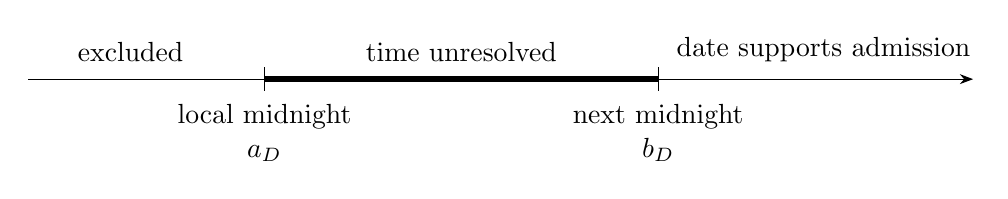
\begin{tikzpicture}[x=1cm,y=1cm,>=Stealth]
\draw[->] (0,0)--(12,0);
\draw[line width=2pt] (3,0)--(8,0);
\draw (3,-.15)--(3,.15) (8,-.15)--(8,.15);
\node[below,align=center] at (3,-.2) {local midnight\\$a_D$};
\node[below,align=center] at (8,-.2) {next midnight\\$b_D$};
\node[above] at (1.3,.1) {excluded};
\node[above] at (5.5,.1) {time unresolved};
\node[above] at (10.1,.1) {date supports admission};
\end{tikzpicture}
\caption{A dated publication supports historical admission only after its
possible publication interval has ended. The line marks uncertainty about an
instant, not a delay imposed on an already known timestamp.}
\end{figure}

Revision selection follows admission. Original selection returns eligible
roots; latest-available selection returns eligible assertions without an
eligible superseding descendant for the same context. Unrelated roots and
multiple live leaves remain competing assertions. A harmonised view adds
explicit transformations with their own admitted sources, method and opening
bridges. File order never selects a winner.

The synthetic interim example has original first-half revenue 120, revised
first-half revenue 110 and revised annual revenue 260. Compatible subtraction
gives second-half revenue $260-110=150$. The arithmetic $260-120=140$ is easy
but mixes incompatible vintages. An original-view display may show both source
amounts while refusing that derived flow. A change in calendar or perimeter
likewise requires a specific bridge.

The financial-amount comparisons investigated so far have not supplied a
qualifying unresolved same-context measurement contradiction. The reference
conflict in Section~\ref{sec:reference-conflict} establishes the narrower
source-navigation finding. Known revisions, different reporting bases and
synthetic conflicts remain useful cases of their own kinds. A financial
conflict case must first match entity, perimeter, concept, dimensions, unit,
basis, period, versions and precision, and investigate extraction and
supersession. The absence of a qualifying measurement conflict in a bounded
search is not evidence that the corpus contains no conflicts.


\section{A revised fact changes a conclusion without rewriting its history}
\label{sec:sector-evidence-revision}

A correction can change the amount that a model now explains while leaving
both its earlier explanation and the company's committed journals intact.
The bank and insurance examples later in this proposal make the distinction
concrete. The bank needs the credit-risk baseline of its irrevocable
commitment even after a loan is drawn. The insurer needs to know whether
its reinsurance treaty preceded the recognition of an onerous group.
Neither fact can be replaced by the time a document happens to arrive.

Consider a constructed bank record that supplies no original commitment
baseline. The analyst can retain its cash flows and conditional loss
scenarios, but cannot establish the required original-to-current credit
comparison. A later record identifies the original commitment risk and
supports the separately supplied finding of significantly increased credit
risk. With the other assumptions in Section~\ref{sec:bank-commitment-draw},
the funded allowance is 4 and equity is 16. The additional record resolves
the missing history; it does not reset the baseline to the draw date.
The relevant AASB~9 provisions retain the irrevocable commitment as the
initial comparison and treat the resulting asset as its continuation
\citep[paragraph 5.5.6 and B5.5.47]{aasb9dated}.
The probability tree remains an authored assumption, and the credit finding
is not inferred merely because a probability doubled.

Suppose, for this constructed record, exact bytes were publicly available
on 2 January, ingested into the system on 5 January, and accepted for the
required reading on 6 January. An investor-information reconstruction with
a 3 January cutoff may use those bytes if their public availability is
verified, even though this particular system obtained them later. A
system-as-of query for 3 January cannot use them. On 5 January a raw
system query may retrieve the document, but a query for an accepted reading
still lacks the 6 January decision. Later extraction is compatible with
the earlier investor cutoff only if its interpretation introduces no later
information. These dates are authored specification fixtures; they
establish no actual historical availability.

\subsection*{A treaty correction separates knowledge from measurement}

In Section~\ref{sec:insurance-connected-groups}, treaty R entered before
group B's recognition produces an initial reinsurance asset of 85,
initial equity of 85 and year-one equity of 83. If R instead enters
immediately afterward, with all other stated facts unchanged, the initial
asset is 70, initial equity is 70 and year-one equity is 74.75.
The loss-recovery recognition condition causes the difference
\citep[paragraph 66A and B119C]{aasb17}. Both histories eventually
reach cash of 88.3 on the same supplied claim and recovery path.
Agreement on that terminal amount therefore cannot establish correct
recognition timing.

Now give the two order assertions different information dates. A constructed
January disclosure says the treaty preceded recognition; a February correction
says it followed recognition and explicitly replaces that order assertion.
A latest-available query cut off in January retains the January assertion.
The February record is known to be too late and cannot suppress it.
A February query may select the correction and produce the later-entry
measurement. The correction concerns the order assertion for B and R;
it does not replace every other assertion in the company's report.

A competing record with unknown public availability has a different effect
from a record known to be published after the cutoff. The known late record
is excluded. The unknown record leaves an unresolved dependency if it might
affect the requested conclusion, even while an older eligible assertion is
displayed. Similarly, an asserted publication date without evidence linking
the retained bytes to that date does not establish historical admission.
If only the common calendar date of treaty entry and group recognition is
known, their order remains unresolved; the model cannot choose 85 merely
because that treatment is more favorable.

An extraction correction is different again. A source may consistently say
that R followed recognition while its first accepted extraction mistakenly
records the opposite. Correcting the reading creates a new reading and
review decision linked to the same source bytes. The old result remains
retrievable as a historical error; reproducing it does not make it correct.
An issuer's correction instead changes the source assertion and usually
its bytes. The system records which change occurred before deciding which
derived results require reassessment.

\subsection*{Invalidate the selection, preserve the committed event}

A result depends on the candidates considered by its selector as well as
the candidate ultimately chosen. Adding a possible competing treaty record
changes that candidate population. Reusing a cached selection solely
because its chosen assertion identifier is unchanged would miss the new
obligation. The proposed dependency graph therefore includes a version for
candidate-set membership. The change propagates from membership through
selection and interpretation to measurement and the resulting statement.
A fresh selection may exclude a known late competitor and calculate the
same amount, but it records that decision under a new view.

Newly created descendants must check their complete ancestry too. Otherwise
a report created after an invalidation scan could inherit a stale measurement
without appearing on the scan's earlier list. In contrast, a bank result whose
complete dependency set contains no changed insurance inputs can remain
reusable. Neither a shared company label nor an unchanged displayed value
establishes independence. Missing ancestors leave reuse unestablished; a
cycle or missing required reference rejects the affected dependency chain.

The retained explanation of a result uses its original evidence view.
It can show a current warning that a dependency has changed, but it cannot
replace the old source with today's correction and still purport to explain
the old calculation. Requesting a different view requires a new calculation.
This preserves the distinction between the company's historical record,
what the system then concluded, and what a later reconstruction supports.

The same rule protects committed accounting events. The connected insurance
example commits financing, service, incurrence and settlement as four
separate events. After settlement, retrying the exact original financing
request returns its original receipt and reports no additional commit;
today's evidence revision does not turn that retry into a new assessment.
Changing the request while retaining the business-event identity is a
conflict. The request's original bindings, historical admission and required
bytes must still validate before receipt lookup.

A new conclusion that the treaty came later does not itself authorize an
entry reducing the committed reinsurance asset. A correction proposal must
identify its accounting treatment, effective period, affected accounts and
opening-balance consequences under the applicable authority. Without that
support, the proposed assessment returns \code{TREATMENT\_UNSUPPORTED},
retains the revised conditional calculation and creates no journal.
Versioning supplies the record of a correction; it cannot supply the
accounting rule that makes the correction appropriate.


\chapter{What the literature contributes}
\label{ch:literature}

The research problem crosses accounting, databases, programming languages,
econometrics and document understanding. Each field resolves part of it. The
review below distinguishes results that can be adopted directly, engineering
ideas that need adaptation, and evidence that does not establish the intended
product capability. Source versions and technical anchors are recorded in the
accompanying research ledgers. The search includes work outside the original
collection, with public-index searches and backward and forward citation
searches through 2 October 2026. It is a scoped design survey, rather than a
claim to enumerate every paper in these fields.

\section{Accounting structure and company dynamics}

\citet{nehmer1997}, especially Sections 2--5, supplies a useful algebraic
starting point: balances occupy a structured state space, transactions change
that state, and aggregation relates detailed accounts to reports. This supports
a distinction between conservation constraints and permitted transactions.
An entry can conserve the accounting total and still be an inadmissible
transaction. AccDSL adopts that distinction in its posting validator. Its
particular event vocabulary, evidence model and inverse-history semantics are
new design decisions, not results established by the algebraic paper.

\citet{doshi2024} develops an accounting DSL with time, transaction logs and
correction mechanisms. The relevant material is in Chapters 4 and 7--9 of the
2024 thesis; the original collection's filename misleadingly suggests 2026.
It demonstrates why corrections and dates belong in the language rather than
in informal comments. The thesis does not establish recovery of an entire
company history from public reports or inference over economically distinct
histories. \citet{babcinetchi2022}, pp.~342--345, offers a much smaller accounting
language and grammar proposal. It is useful as a syntax precedent, but it
provides insufficient semantics or evaluation to govern AccDSL by itself.

\citet{shahnazarian2004} connects accounting dynamics with behavioural and
econometric equations. Sections 2.3--2.8 describe the accounting relationships;
the optimisation and econometric discussion in Chapter 3 and the data and
evaluation material in Chapters 4 and 8 show how the model is used with
standardised Swedish corporate data. This is an important precedent for
simulating companies under changed conditions. Its standardised tax-data
starting point differs from heterogeneous public-report extraction, and its
working-capital funds formulation should not be imported as a general modern
cash-flow statement implementation. The transferable idea is the explicit
separation of accounting evolution and behavioural assumptions.

\citet{pierson2020}, Sections 3--4 and the reporting structures, makes that
separation operational in system dynamics. Receivables, payables and wages
accumulate differences between accrual and payment flows; reporting-period
accumulators turn instantaneous flows into statements. AccDSL can use these
structures as examples of coherent movement schedules. The model's payment
delays, inventory approximations and simplified equity treatment remain
modelling choices. They are not universal defaults for companies or evidence
that an aggregate state is sufficient for all shocks.

Bank models demonstrate why journal generation needs economic state.
\citet{halaj2016}, Section 3, combines funding shocks, fire sales, loans,
securities and risk constraints. The homogeneous portfolios and specified
funding process make the model tractable, but limit instrument-level
interpretation. \citet{behn2019}, Section 2, makes managers' choices over asset
growth, debt, risk and payouts depend on capital and liquidity constraints.
These models motivate interfaces for management policy and regulatory
calculations. Their parameterisations must be calibrated and evaluated for
the target application; passing their accounting identities would not validate
an AccDSL forecast.

Two important neighbouring traditions remain explicit coverage qualifications.
McCarthy's 1982 REA model is a foundational candidate for the relation between
resources, events and agents; Caiani and co-authors' stock-flow-consistent
agent-based benchmark is a candidate for simulation across interacting sectors.
Verified primary PDFs could not be obtained in this retrieval campaign after
institutional and publisher attempts. Their records are retained in the omission
register, and no technical result from either is used to justify the design.
AccDSL's event and counterparty records are specified and justified in Chapters~\ref{ch:language} and~\ref{ch:execution}. A later multi-company equilibrium engine would require expansion of
the stock-flow-consistent literature before implementation.

\section{Incomplete information and provenance}

Financial disclosures are incomplete databases in a substantive sense.
Multiple underlying records can yield the same published observations.
\citet{libkin2014}, Sections 2--6, explains the semantics of incomplete
databases, labelled nulls, conditional tables and certain answers. Repeated
occurrences of the same unknown must share a value. Conditional tables can
represent dependence between alternatives that independent missing cells
cannot express. This is directly relevant to a debt note and a cash-flow table
that refer to the same unknown repayment.

AccDSL adopts shared symbolic unknowns and conditions. It extends the database
idea with accounting constraints, continuous amounts, temporal transitions and
economic event models. A ``certain'' answer means a statement that holds for
every history in a nonempty declared feasible family. This is Boolean
certainty; a table of individually certain rows can lose existential
information and must not imply that omitted rows are absent. The payable
example in Section~\ref{sec:query-certainty} develops this distinction.
The family itself may omit
unknown mechanisms; certainty is therefore always relative to a model scope.
Imieliński and Lipski's original 1984 paper is a foundational backward lead
whose publisher copy was inaccessible in this campaign. The inspected Libkin
paper supplies the technical discussion actually used here.

\citet{green2007}, Definitions 3.1--3.2 and Section 4, treats provenance as
annotations that compose through relational operations. Combining sources
and alternative derivations can therefore have formal semantics, rather than
being a list of unrelated citations. This is useful for report aggregation and
explanation queries. Positive relational operations covered by provenance
semirings do not by themselves specify every operation AccDSL needs: negation,
nonlinear valuation, optimisation and probabilistic conditioning require their
own derivation records. Accordingly, the implementation starts with a typed
dependency graph and may use semiring annotations for supported relational
subqueries. A dependency edge is not a posterior probability.

\citet{snodgrass1986} distinguishes historical validity from the time facts
are stored. The archived paper is \emph{Temporal Databases}, by Snodgrass and
Ahn, not the later Jensen--Snodgrass paper initially returned by a search.
Its snapshot, rollback, historical and temporal examples support the need to
recover both old business facts and old database beliefs. AccDSL adds public
availability time because a database insertion date cannot establish whether
a historical investor could have seen a filing.

\section{Inverse problems, identification and probability}

\citet{stuart2010}, Section 2.2, starts from an observation equation
$y=G(u)$ and distinguishes inversion, regularisation and Bayesian inference.
The discussion makes explicit that a regularising norm or prior is an
additional assumption. AccDSL has a similar observation problem, although
its unknowns include discrete accounting interpretations and event structures
as well as continuous parameters. The infinite-dimensional well-posedness
theorems in that paper are not automatically applicable to this mixed,
potentially discontinuous model.

The relevant issue is often identification rather than computation alone.
\citet{giacomini2021}, Sections 2.1--2.6 and Theorem 1 of the archived 2020
working version, shows how a class of priors can preserve uncertainty within
an identified set. A likelihood that is flat over the unresolved part does
not learn the conditional prior over that part. Posterior lower and upper
probabilities summarise a class of posterior beliefs. The paper's regularity
conditions and application to structural vector autoregressions do not prove
that an arbitrary accounting program admits the same algorithms or guarantees.
The design borrows the distinction between learnable quantities and
assumption-dependent distributions; the simple accounting bounds in
Chapter~\ref{ch:math} are derived directly.

\citet{hoeting1999}, equations (1)--(3), gives Bayesian model averaging as a
weighted sum of model-conditional distributions, with weights determined by
model priors and marginal likelihoods. Sections 3 and 5 discuss computation
and prior specification. This supports an optional weighted mode, provided
AccDSL specifies the likelihood, priors and candidate model space. It does
not justify giving equal mass to every syntactically different journal
reconstruction. Two encodings of the same economic history must not gain extra
weight by duplication. Model averaging also remains conditional on the
considered model family, rather than repairing missing mechanisms.

Scenario semantics need similar care. \citet{pearl2009}, Section 3.2.1 and
equations (5)--(6), distinguishes an intervention that replaces a structural
equation from ordinary conditioning. AccDSL will distinguish a supplied
exogenous path, an observational conditional forecast and an intervention.
A rise in rates imposed by a stress test is not automatically distributed as
the collection of historical periods in which rates happened to be high.
Identifying a causal effect requires assumptions beyond reproducing accounts.

\section{Languages for rules and contracts}

\citet{vandeursen2000} surveys DSL benefits, risks and implementation options.
\citet{mernik2005}, Sections 1.1 and 2.2--2.5 of the archived CWI report,
treats application libraries as serious competitors and distinguishes deciding,
analysing, designing and implementing a DSL. Its implementation decision tree
explicitly includes embedding in a host language. The literature therefore
supports a conditional design decision: a DSL is attractive when domain
constraints and repeated notation justify it, but an ordinary typed library
may be cheaper and equally expressive. AccDSL will implement one shared
representation accessible from both a Python API and a textual language, so
syntax does not become a prerequisite for testing the accounting model.

\citet{merigoux2021}, Sections 3--4 and Figures 8--9, provides Catala's scopes,
exceptions, default calculus and translation into a conventional functional
target. Its explicit empty and conflict outcomes are valuable precedents for
accounting rules with exceptions. They are different from probabilistic
uncertainty. AccDSL will preserve this distinction: conflicting applicable
rules produce a diagnostic, while an evidence-supported alternative reading
produces a conditional model branch. The paper's compiler correctness results
do not establish correctness of our accounting rules or of an automatic
translation from disclosures.

The inspected LegalMath code offers reusable ideas in its shared typed
interpretation, partial observations, source references and validity/knowledge
times. Its ordinary frontend execution selects a reading. AccDSL needs an
additional execution mode that retains a family of readings, continuous
unknowns and economic state. A bounded candidate generator is useful for
search, but its candidate limit does not prove completeness.

\citet{jones2000}, Sections 3--5, builds complex financial contracts from
combinators and separates their compositional meaning from a chosen valuation
model. The ACTUS technical specification similarly separates contract states,
scheduled events, state transitions and payoffs, with risk factors supplied
through an interface \citep{actus}. These are strong reasons to represent
contractual obligations independently of accounting classifications. Neither
contract cash flows nor a derivative price determine the recognition,
measurement and presentation rules of a complete IFRS or US GAAP book.

\section{Extraction and financial reasoning}

The document literature supports a staged ingestion process. PubTables-1M
\citep{smock2022}, in its canonicalisation procedure and evaluation section,
distinguishes table detection, structure recognition and functional analysis.
Its GriTS evaluation compares reconstructed table structure. TableBank
\citep{li2020}, Sections 3--4, uses document structure to obtain weak supervision
for table detection and recognition. GTE and FinTabNet \citep{zheng2021},
Sections 3--5, provide a financial-document setting and company-level dataset
splits. These sources help select extraction components and evaluation units.
Their table scores do not establish that a debt note has been interpreted
correctly across years or that every off-balance-sheet exposure has been found.

The Docling report \citep{nassar2024}, Section 3, describes PDF parsing, page
layout analysis and table structure recognition within a document-conversion
pipeline. The locally archived version lists Christoph Auer first; this
version difference is recorded in the catalogue. Docling is an ingestion
candidate whose output must retain source locations and undergo accounting
validation. Its code and model licences must be considered separately when
packaging a deployment.

\enlargethispage{\baselineskip}
TableFormer makes the division between structure and text concrete.
\citet{nassar2022tableformer}, Sections 4--5, describe a model that receives a
cropped table image and predicts its HTML structure together with a bounding
box for each cell. The cell's words and numbers come from separately supplied
PDF text; they are not generated by the structure decoder. Matching the
predicted cells to that text is itself consequential. The supplementary
algorithm can remove duplicate columns, attach previously unmatched text to a
cell, or create a new cell \citep[Section 2]{nassar2022tableformersupp}. A
plausible grid therefore still needs its text assignments and structural
corrections checked against the source.

The paper's evaluation preserves this distinction. Table 4 reports TEDS,
a similarity measure based on tree edit distance, for structure \emph{with
content} on PubTabNet PDF documents containing cropped tables: 95.4 for simple
tables, 90.1 for complex tables and 93.6 overall. The content comes from PDF
cells; Table 2 separately reports structure-only results
\citep[Tables 2 and 4, p.~4620]{nassar2022tableformer}. These are results for
that input population and text supply. They do not establish extraction
accuracy for complete financial filings, or whether a cell has been assigned
the correct entity, period, unit or accounting meaning. Those questions require
the source-linked accounting checks developed here.


FinQA \citep{chen2021}, Sections 3--6, provides questions with executable
reasoning programs and supporting evidence. TAT-QA \citep{zhu2021}, Sections
2--4, combines table cells and text spans with aggregation operations, and
explicitly treats numerical signs in evaluation. DocFinQA \citep{reddy2024}
extends financial questions to long documents and evaluates retrieval/context
choices. FinBen \citep{xie2024} broadens the collection of financial tasks and
model evaluations. These benchmarks can test retrieval and local numerical
reasoning. Their question-answer format does not require a complete
multi-period company representation, joint alternative histories or
scenario-dependent journal generation.

A directly relevant recent competitor is the auditable RAG architecture of
\citet{cosentino2026}. Sections 3.1--3.2 describe persistent extraction,
enrichment, retrieval and provenance records; Section 4.6 checks citation
resolvability and failure recovery. Section 5 limits the interpretation of
those results to the evaluated document-intelligence tasks. AccDSL should
reuse the idea of persistent evidence and recoverable processing, while adding
executable accounting and economic semantics. No performance comparison with
that architecture has been run here.

\section{Solvers and probabilistic execution}

\citet{damoura2008}, Sections 2--3, describes Z3's interfaces and theory-solving
architecture. It supports choosing an SMT solver for logical choices and
arithmetic constraints, but does not make arbitrary nonlinear simulation
tractable. The first solver fragment is deliberately bounded: finite choices,
exact linear arithmetic and selected calendar relations. Unsupported formulas
remain in the representation with a solver diagnostic.

\citet{vandeMeent2018} develops probabilistic programs through sampling,
observations and inference; the inspected material includes the first-order
language and weighted sampling discussion. Stan \citep{carpenter2017}, its
model language and sampler-output discussion, and Pyro \citep{bingham2019},
Sections 2--3, show different ways to separate a probabilistic model from
inference machinery. They are candidates for optional inference over an
already-defined economic model. Exact accounting identities and discrete rule
selection should not be turned into nearly satisfied likelihood penalties
merely to fit an inference library. Nor should successful sampler execution
be described as evidence that all interpretations were explored.

\clearpage
\section{The remaining design problem}

The combined literature provides algebra for journals, semantics for missing
information, temporal storage, provenance, contract languages, rule languages,
inference methods and extraction tools. The unresolved integration problem is
to retain their distinctions while connecting them: a disclosure constrains
economic histories; a history supplies contract and behavioural state; a
scenario drives events; accounting rules produce journals; reporting rules
render statements; and every step remains explainable.

The design is therefore an integration proposal with several local
mathematical constructions. Its originality and empirical advantage have not
been established by this survey. Its practical merit will depend on the
acceptance cases, accounting review and comparative implementation work in
Chapter~\ref{ch:validation}.

\chapter{Architecture and reuse}
\label{ch:architecture}

\section{One representation, several authoring methods}

The architectural centre is a typed intermediate representation (IR), not a
text parser. A document extractor, a human editor, a Python library and the
AccDSL compiler all create the same records. This allows a modeller to begin
with a reviewed structured file and later add convenient notation. It also
allows source extraction to improve without changing accounting semantics.

\begin{figure}[ht]
\centering
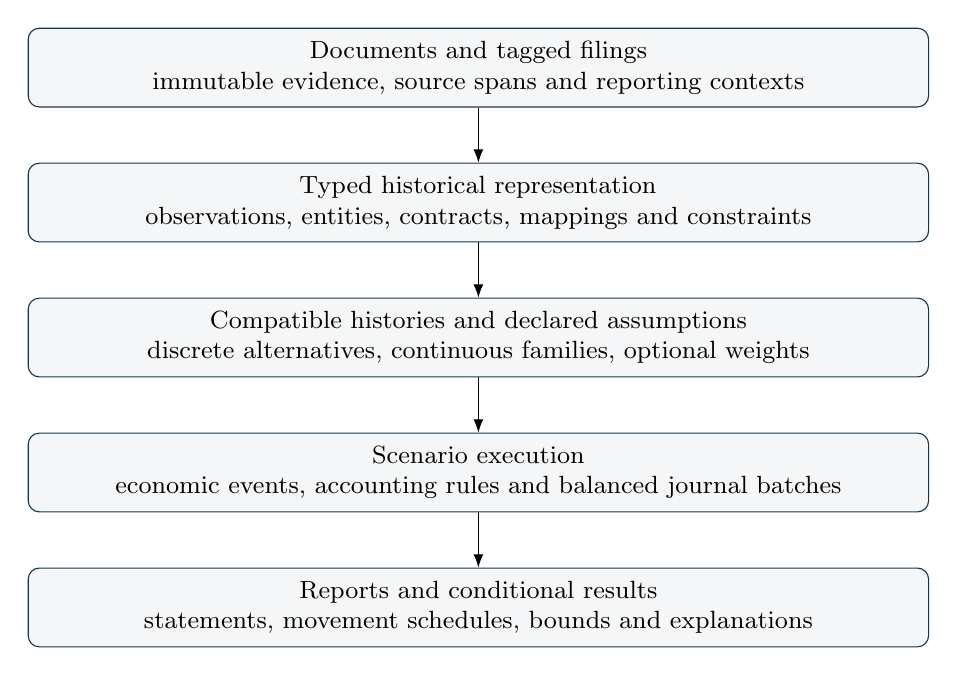
\begin{tikzpicture}[node distance=7mm,>=Latex,
 box/.style={draw=ink,rounded corners,align=center,text width=112mm,
 minimum height=10mm,font=\small,fill=papergray}]
\node[box] (e) {Documents and tagged filings\\immutable evidence, source spans and reporting contexts};
\node[box,below=of e] (h) {Typed historical representation\\observations, entities, contracts, mappings and constraints};
\node[box,below=of h] (i) {Compatible histories and declared assumptions\\discrete alternatives, continuous families, optional weights};
\node[box,below=of i] (s) {Scenario execution\\economic events, accounting rules and balanced journal batches};
\node[box,below=of s] (r) {Reports and conditional results\\statements, movement schedules, bounds and explanations};
\draw[->] (e)--(h);\draw[->] (h)--(i);\draw[->] (i)--(s);\draw[->] (s)--(r);
\end{tikzpicture}
\caption{The simulation path. Every transformation records its inputs and
assumptions; the source record remains available throughout.}
\label{fig:architecture}
\end{figure}

Evidence storage and economic modelling must remain separate. If a company
reports 100 of borrowing, a model can assume two loans of 60 and 40 without
creating a new reported fact that the company disclosed those loans. The
contract library consumes the assumed terms, the accounting module consumes
the resulting events, and the explanation graph records the assumption at
each affected result.

\section{Why a DSL, and when another approach is better}

The strongest baseline is a typed schema, SQL storage and ordinary Python
code. That combination can implement the whole product. Its disadvantage is
that repeated accounting requirements can become conventions scattered across
functions: implicit currency conversion, missing period checks, hidden default
values and duplicated rule selection. A bounded language makes these
requirements part of typing and compilation. Its costs are language
maintenance, diagnostics, migration and training.

\begin{longtable}{L{29mm}L{51mm}L{56mm}}
\toprule Approach & Useful role & Limitation for this product\\\midrule\endhead
Typed schema and Python & Reference executor, flexible economic models,
initial authoring API & Domain restrictions require disciplined APIs or a
validator; arbitrary code complicates static analysis and provenance.\\
XBRL and OIM & Tagged evidence, contexts, dimensions, taxonomies and exchange &
Reported facts and reporting relationships do not recover hidden economic
histories or specify scenario behaviour.\\
Ledger languages & Recording known transactions, balance checks, export and
differential testing & Alternatives, source interpretation and contract
exposure need additional semantics.\\
Knowledge graph / SQL & Relationships, lineage, temporal queries and evidence
navigation & A graph or schema alone does not define event execution or the
probability meaning of alternatives.\\
Rules / Catala & Dated policy logic, defaults, exceptions, traceable rule
evaluation & Ledger state, event scheduling and ensembles require an enclosing
runtime.\\
Probabilistic program & Priors, likelihoods and inference over model parameters &
Needs declared probability measures; cannot turn unspecified ambiguity into
probability or supply accounting rules.\\
Spreadsheets & Familiar review and small transparent financial models &
Versioned evidence, shared unknowns and branching histories are difficult to
govern as the model grows.\\
AccDSL over shared IR & Common domain checks, reusable templates, explicit
alternatives and deterministic posting semantics & Requires implementation and
evaluation; broad notation without stable semantics would add cost.\\
\bottomrule
\end{longtable}

The decision is to implement the IR, validators and Python reference API first,
then the textual frontend. The same conformance cases must pass through both
frontends. If the DSL fails to reduce ambiguity in representative authoring
tasks, the IR and library remain useful. This is a reversible product decision,
not a claim that a new language is inherently better than a library.

\section{Open-source components}

The following survey uses official repository descriptions, licence files and
selected source interfaces archived on 2 October 2026. It is a source
inspection, not an executed integration or performance evaluation. The
machine-readable tool ledger records retrieval paths and available version
metadata. Dependencies must be pinned when implementation begins; a branch
name observed during this survey is not a release requirement.

\begin{longtable}{L{26mm}L{71mm}L{39mm}}
\toprule Component & Proposed use and checked boundary & Licence / decision\\\midrule\endhead
Arelle & Parse and validate XBRL/iXBRL. Inspected \code{ModelFact}, context and
unit accessors. Preserve taxonomy extensions and full contexts when importing.
& Apache-2.0 core; first-choice adapter.\\
Docling & PDF layout, text and table conversion. Inspected converter interface;
retain page coordinates and extraction settings. & MIT code; assess model
licences separately. Candidate.\\
Table Transformer & Table extraction baseline associated with PubTables-1M;
check finance-domain performance before selection. & MIT; repository marked
archived in inspected metadata. Baseline, not a maintenance default.\\
Beancount & Posting and transaction data types; export selected concrete
branches and compare balances. & GPL-2.0 project metadata; integration and
redistribution choice needed. Optional adapter.\\
Ledger & Known-journal reference and export. Inspected transaction balancing
code and manual date/assertion behaviour. & BSD-style licence; optional
reference tool.\\
hledger & Alternative ledger import/export and accounting checks. Repository
documentation inspected. & GPL-3.0 project metadata; optional process adapter.\\
Catala & Potential backend for deterministic policy modules; defaults and
exceptions have useful semantics. & Apache-2.0; prototype only after core
execution semantics stabilise.\\
ACTUS & Contract schedules, payoffs and transitions; external risk-factor
interface. Verify event schedules against ACTUS tests. & Service Apache-2.0;
technical specification CC-BY-SA-4.0. Candidate contract adapter.\\
QuantLib & Calendars, cash flows and valuation. Floating coupon source separates
fixing dates and pricing. Accounting treatment remains external. & Modified
BSD-style licence; candidate valuation adapter.\\
OpenFisca & Versioned tax-benefit formulas as a rule-system reference; inspected
variable/formula metadata. Corporate-tax coverage must be supplied. & AGPL-3.0;
optional, not the core runtime.\\
Z3 & Finite alternatives, logical compatibility, linear constraints and conflict
explanations. & MIT licence text; first solver candidate.\\
DuckDB & Local analytical queries over extracted facts and results. & MIT;
candidate alongside SQLite transactional storage.\\
Stan & Continuous probabilistic models and diagnostics with an explicit target.
Inspected model interface and paper. & BSD-3-Clause; optional inference backend.\\
Pyro / PyMC & Alternative probabilistic backends for model-specific inference.
Pyro design paper and project descriptions inspected. & Apache-2.0 / Apache-2.0
licence texts; optional, no default selection.\\
\bottomrule
\end{longtable}

The licence entries identify the inspected projects, not a legal conclusion
about every combination of code, models and datasets. The default product
architecture can communicate with optional tools through explicit adapters.
This does not, by itself, settle redistribution obligations. That question is
resolved when a concrete dependency and distribution method are selected.

XBRL's Open Information Model supplies standardised facts with concepts,
entities, periods, units and dimensions \citep{xbrloim}. Those facts are an
excellent ingestion source. AccDSL retains their original contexts and
decimals rather than flattening them immediately into a company-by-year table.
Calculation relationships can help validate reporting totals, but are not a
general description of the transactions that generated those totals.

\section{Responsibilities that AccDSL must implement}

AccDSL owns the evidence and temporal model, typed accounting concepts, shared
unknowns and alternatives, rule-package selection, journal validation,
consolidation provenance and report explanations. It also owns the distinction
between feasible sets and distributions. These responsibilities cannot be
delegated implicitly to whichever parser or solver is convenient.

External components receive narrow requests and return typed responses.
A contract adapter returns scheduled events, cash-flow quantities, state
changes and source/model references; it does not directly mutate the ledger.
A valuation adapter returns a measure, currency, date, method and numerical
status; the accounting package decides whether and where to recognise the
change. A solver returns feasibility or bounds with scope and completeness
status. A language model proposes source-linked mappings or interpretations;
it cannot commit an unsupported assertion as fact.

The architecture consequently permits deterministic reference execution,
alternative solvers and later acceleration without changing the meaning of a
historical observation or a journal entry. Performance work begins only after
the same semantic cases pass through these interfaces.

\chapter{Historical compatibility and future simulation}
\label{ch:math}

\section{Define what is observed before inverting it}

Let $D_k$ be the disclosures available under information cutoff $k$. Each
numeric observation $d_i$ has a context: entity or group perimeter, concept,
measurement basis, dimensions, currency, period and precision. These contexts
are part of the observation operator, not additional columns that can be
discarded after extraction.

A candidate history $h$ contains an opening economic and accounting state,
events through the last historical date $T$, contract terms, accounting
policies, consolidation relationships and latent quantities. Let $M$ denote
the declared model scope: its event templates, admissible rule versions and
allowed unknowns. It excludes arbitrary events that the chosen model has no
way to represent. The reporting operator $O_i(h)$ produces the quantity to
which observation $i$ refers, including its basis and perimeter.

Reported numbers are often rounded. If a number $v_i$ is rounded to the nearest
unit $q_i$, an illustrative admissible interval is
$[v_i-q_i/2,v_i+q_i/2)$ under the corresponding tie convention. This
half-open endpoint choice is used only when that tie rule is declared;
Section~\ref{sec:source-rounding} gives the conservative closed enclosure when
nearest rounding is assumed but the tie rule is unknown. The actual
rounding convention, scale and XBRL accuracy metadata govern the imported
constraint. A disclosure with unspecified precision does not acquire a
convenient tolerance silently. Write $\mathcal{I}_i$ for the justified
observation interval, and $C_M(h)$ for the joint accounting, contractual and
semantic constraints. Then the historical compatibility set is
\begin{equation}\label{eq:histset}
 \Hist_M(D_k)=\{h\in\mathcal{H}_M:
 C_M(h)\ \land\ O_i(h)\in\mathcal{I}_i\text{ for every applicable }i\}.
\end{equation}
Qualitative assertions enter as reviewed logical conditions, rather than
numeric intervals. Incompatible source contexts are never forced into the
same equation.

Equation~\eqref{eq:histset} distinguishes three outcomes. An empty set means
that the observations and declared model are inconsistent. A singleton means
that this model identifies a history at its chosen resolution. A larger set
preserves unresolved alternatives. An empty set does not prove that the
company's accounts are false: a wrong extraction, missing event type or
incorrect perimeter can cause the inconsistency. A singleton does not prove
that the model contains the real history.

\section{A certain liability need not identify its creditor}
\label{sec:query-certainty}

Suppose the admitted records establish exactly one payable of 100 currency
units, but leave its creditor unresolved between A and B. For this constructed
example the declared family has two histories: in $h_A$ the company owes A
100 and owes B nothing; in $h_B$ it owes B 100 and owes A nothing. These are
complete alternatives within the example, not two sampled points from a wider
family. The question \emph{does a payable exist?} has the answer yes in both
histories. The question \emph{is A owed 100?} does not.

Now ask for the rows of the payable schedule. If $Q(h)$ returns those rows,
then $Q(h_A)=\{(A,100)\}$ and $Q(h_B)=\{(B,100)\}$. Their intersection is
empty: no creditor--amount row occurs in both. Reading that empty table as
the company's complete schedule would wrongly assert that it owes nothing.
Reading the union as its complete schedule would instead assert that it owes
200. Evaluating the total within each history gives 100 in both. The
uncertainty concerns the creditor, not the existence or total of the payable.

This distinction is central to Libkin's critique of intersection-based
answers. His example retains a tuple with an unknown second component;
discarding it loses knowledge that a tuple with the stated first component
exists. An intersection read under a closed-world interpretation can also
add an unsupported absence claim \citep[Section~3 and the opening of
Section~6]{libkin2014}. A table of individually certain rows is therefore a
restricted view of knowledge, not generally a replacement for the possible
answer schedules.

For a nonempty feasible history family $H=\Hist_M(D_k)$ and a total,
deterministic query $Q$ on its histories, retain the family of answers
\[
 \mathcal{A}_Q(H)=\{Q(h):h\in H\}.
\]
Each answer remains linked to the histories that produce it. Equality of
payable schedules alone does not license merging histories for another query.
For a row-valued query, a separately requested certain-tuples view is
\[
 T_Q(H)=\bigcap_{h\in H}Q(h).
\]
Membership in $T_Q(H)$ asserts that a row appears in every answer. Omission
asserts only that the row is not established in every answer; it does not
assert absence from every answer. A total computed after taking this
intersection answers a different question from totals computed within
histories. In the payable example, $T_Q(H)$ is empty while
$\{\operatorname{total}(Q(h)):h\in H\}=\{100\}$.

For a proposition $P$ about a concrete answer, Boolean certainty has the
separate meaning
\[
 \operatorname{Certain}_H(P\circ Q)
 \quad\Longleftrightarrow\quad
 \forall h\in H,\ P(Q(h)).
\]
Taking $P$ to mean that the schedule contains at least one payable proves
existence without identifying A or B as the creditor. Allowing a third history
with no payable would change that answer. The two-history result consequently
depends on the admitted evidence and scope that require the liability to
exist, not merely on the two rows chosen for display.

Libkin distinguishes a logical description of knowledge shared by all
answers from an object representing their greatest lower bound in an
information ordering. These representations need not exist in the chosen
language; ordinary tuple intersection is not their general definition
\citep[Section~5.3, equations~(6)--(8)]{libkin2014}. AccDSL's answer family and
Boolean propositions above are local definitions. They do not assert that
every family has a finite relational representation. A symbolic answer must
carry its conditions and preserve the stated family, or declare the
restriction or approximation it makes.

Input completeness and output meaning must also be explicit. A model that
fixes the available event templates and contract slots imposes a scope
restriction; it does not establish that a public filing lists every economic
event. Nor does that restriction entitle a display to interpret every omitted
row as false.

Libkin's primary proof compares information by reverse inclusion of possible
completions: an object is more informative when fewer complete objects remain
compatible with it. For a query to be evaluated directly on an incomplete
object, the chosen output interpretation must preserve that order as input
information increases. The query must also respect the relevant renamings,
and its output domain must have a representation system whose formulas
describe each object's complete interpretations
\citep[Sections~6.1--6.2, equations~(9)--(10)]{libkin2014}. In Theorem~2, the proof
first shows that evaluating the query preserves exactly the statements true
in all completed answers; it then uses those statements to establish the
greatest-lower-bound answer as an object
\citep[Definitions~4--7 and Theorem~2, pp.~11--18]{libkin2016certain}.
Monotonicity alone is insufficient, and SQL null comparisons need not meet
the genericity condition \citep[Section~7.1, pp.~18--19]{libkin2016certain}.

The relational examples make the difference between input and output
assumptions concrete. Positive existential queries have the stated result
with open-world inputs and answers. A guarded positive fragment also has it
with \emph{closed-world inputs and open-world answers}; the latter is an
interpretation of omitted result rows, not a claim that the input filing
lists every economic event
\citep[Proposition~9 and Corollary~3, p.~20]{libkin2016certain}.
These results do not authorize evaluating arbitrary financial negation,
aggregates or nonlinear constraints by treating unknown amounts as ordinary
constants. AccDSL has not established the theorem's abstract domain,
information order and representation-system conditions for every financial
output. The constructed payable example above instead follows directly
from its two declared histories.

A related relational method illustrates what a sound but incomplete answer
means in practice. For marked-null tables under closed-world set semantics,
Libkin's modified three-valued evaluator returns a certainly positive answer
when it yields 1 and a certainly negative answer when it yields 0; its value
$1/2$ carries no guarantee \citep[Theorems~4.1 and~5.3, pp.~8--12]{libkin2016sql}.
Let $T=\{(1,\bot)\}$ and ask whether there is a $y$ for which $T(1,y)$ and
either $y=1$ or $y\ne 1$. Every completed table answers yes, yet the modified
evaluation leaves the answer at $1/2$: its null comparison and its negation
are both unknown. The paper gives this case as a missed certain answer for
ordinary SQL; the modified evaluator's outcome follows from its atomic rules.
An inconclusive evaluation therefore does not show that two possible histories
give opposite answers. AccDSL requires witnesses on both sides to establish
that stronger claim; a timeout or unsupported operation remains undecided.
The relational guarantee itself does not transfer to financial totals,
nonlinear valuations, temporal histories or scenario conditioning.

The query contract records whether it returns a proposition, individually
certain rows, or a family of answers, together with the family scope and
completeness and the interpretation of omitted rows. Unsupported evaluation
and unfinished search keep their existing failure or unresolved status. In
particular, a sampled answer family cannot be relabelled as the full family
merely because its displayed rows agree.


\section{Why published statements cannot identify all transactions}

The simplest derivation uses fixed account mappings and a fixed basis. Let
$z\in\mathbb{R}^n$ contain unknown historical movement amounts. For $m$
disclosed aggregates, let $A\in\mathbb{R}^{m\times n}$ be the aggregation
matrix and $y=Az\in\mathbb{R}^m$. If there is a nonzero vector $v$ with
$Av=0$, then
\[
 A(z+v)=Az+Av=y.
\]
Both movement vectors give the same reports whenever both satisfy the remaining
constraints. Thus the feasible family is the affine set $z+\ker A$ intersected
with those constraints. Accounting requirements can shrink this family, but
do not generally eliminate it. For example, cash collections in a receivables
bridge are constrained by
\[
 AR_T=AR_0+\text{credit sales}-\text{collections}
       -\text{write-offs}+\text{other classified movements}.
\]
If the note does not distinguish acquisitions, currency effects and write-offs,
several collections paths may fit the same closing balance.

There is a second ambiguity beyond aggregation. In
Equation~\eqref{eq:running}, identical historical movements arise from different
contractual reset terms. Even recovering $z$ exactly would leave these terms
unidentified. AccDSL therefore infers economically relevant states and
contract terms alongside journal movements. A linear inverse solver over
statement lines alone cannot solve this second problem.

\section{The accounting state and its invariants}

For one entity book with $n_a$ accounts in one functional currency, let
$b_t\in\mathbb{Q}^{n_a}$ be
signed account balances, with debit amounts positive and credit amounts
negative. Exact decimal amounts can be represented as rationals with a power
of ten denominator. A journal batch $j_t$ contains the signed functional-currency
amounts posted by one atomic event or explicitly grouped event batch. Its
balance condition is
\begin{equation}\label{eq:posting}
 \boldsymbol{1}^{\mathsf T}j_t=0,\qquad b_t=b_{t^-}+j_t.
\end{equation}
If $\boldsymbol{1}^{\mathsf T}b_0=0$, substitution gives
$\boldsymbol{1}^{\mathsf T}b_t=
\boldsymbol{1}^{\mathsf T}b_{t^-}+\boldsymbol{1}^{\mathsf T}j_t=0$.
Induction establishes conservation through every committed batch. Opening
balances must therefore be supplied as a balanced, explained entry or a
balanced imported state with unresolved composition explicitly identified.

This proof establishes a bookkeeping invariant. It does not establish that an
amount belongs in the chosen account, that a contract exists, or that an
accounting standard permits a treatment. Posting validation additionally
checks account roles, ownership, currency conversions, applicability of rules
and event preconditions.

The balance vector includes temporary revenue and expense accounts during
the period. Period closing transfers their net balance to equity through
balanced entries. A reporting function can include current profit in equity
before closing, or use the closed book afterwards, but must not include it
twice. Income and cash-flow reports use classified movements and exclude
mechanical closing transfers from operating flows. Consequently statements
are functions of balances, journals, contract state and reporting rules:
\begin{equation}\label{eq:report}
 Y_{[u,v)}=R(b_{v^-},J_{[u,v)},X_{v^-},\rho,[u,v)).
\end{equation}
Here $\rho$ specifies the reporting basis and perimeter, and $X$ contains
economic state beyond ledger balances. Cash-flow classification is part of
$R$, not recoverable from the closing cash balance alone.

Each book has its own functional currency. Quantities such as shares, tonnes
and foreign-currency units are typed separately and never added to this
balance equation. A foreign-currency posting stores its original units and
the functional-currency valuation with its rate source. Translation into a
group's presentation currency and consolidation adjustments occur in a
separate book under explicit rules.

\section{Simulate events from economic state}

For a chosen history $h$, the state at $T$ is $X_T(h)$. It contains balances,
open contracts, lots or cohorts, unpaid accruals, commitments and other
quantities needed for future evolution. Let $s$ identify a scenario definition,
$U_t^s$ its supplied economic drivers, $a_t$ management's actions, and
$\varepsilon_t$ future innovations. A behavioural policy $\pi$ chooses
$a_t$ using the permitted information $\mathcal{F}_t$:
\begin{align}
 a_t&=\pi(X_t,U_{\leq t}^s,\mathcal{F}_t;\theta),\label{eq:actions}\\
 e_{t+1}&=\mathcal G(X_t,a_t,U_{t:t+1}^s,\varepsilon_{t+1};\theta),\label{eq:events}\\
 (j_{t+1},m_{t+1})&=\mathcal A(e_{t+1},X_t,r_{t+1}),\label{eq:account}\\
 X_{t+1}&=\mathcal T(X_t,e_{t+1},j_{t+1},m_{t+1}).\label{eq:transition}
\end{align}
The generator $\mathcal G$ emits events, such as a sale, rate reset, payment or default.
The accounting function $\mathcal A$ applies rule package $r$ and returns journal
postings plus measurement annotations $m$. The transition $\mathcal T$ updates economic
and ledger state atomically. A default can therefore change the loan's legal
status, expected recoveries, recognised allowance and cash collections through
related, but distinct, records.

This ordering is a reference abstraction. Within a date, event dependencies
and phases specify the actual order. Expectations used to measure an allowance
or provision must be calculated from the information permitted at that date.
They cannot use the realised future path of the simulation. An inner
expectation model may use quadrature, analytic formulas or nested simulation;
its approximation and seed belong in the measurement annotation.

Some scenarios specify a deterministic macroeconomic path while leaving
idiosyncratic defaults random. Others supply a joint stochastic driver model.
A risk-neutral measure used to value a derivative is distinct from the
real-world measure used to simulate business outcomes. Every stochastic
adapter declares its measure and conditioning information. The accounting
function receives the resulting valuation with that declaration.

\section{Preserve sets and distributions separately}

Let $K_{h,s}$ be the probability law of future reports produced by the forward
model conditional on history $h$, scenario $s$ and its declared behavioural
assumptions. A deterministic simulation is the special case of a point mass.
When no probabilities over historical explanations are justified, the natural
answer is a family of laws,
\begin{equation}\label{eq:family}
 \mathcal{K}_{M,s}(D_k)=\{K_{h,s}:h\in\Hist_M(D_k)\}.
\end{equation}
The system can report each explanation, bounds on a deterministic outcome,
or lower and upper event probabilities across this family. Those are different
result types. A range of conditional means is not a confidence interval, and
an envelope of conditional quantiles is not itself a single predictive
distribution.

If a defensible probability measure $\mu(dh\mid D_k,M)$ supported on
$\Hist_M(D_k)$ is supplied, histories and report outcomes must have specified
measurable spaces. Assume that $K_{h,s}$ is a probability kernel: it is a
probability measure on report outcomes for each $h$, and $h\mapsto K_{h,s}(B)$
is measurable for each measurable event $B$. The predictive law is then
\begin{equation}\label{eq:mixture}
 \Prob(Y^s\in B\mid D_k,M)=
 \int K_{h,s}(B)\,\mu(dh\mid D_k,M).
\end{equation}
For discrete explanations this is the usual weighted sum. For continuous
unknowns, integration uses the declared measure over those unknowns, not a
count of solver solutions. Bayesian weights require a prior and a likelihood;
expert weights remain labelled as elicited. A likelihood must not treat a
statement total and all its components as independent repeated evidence.
Deterministic equality constraints require a reduced parameterisation or
proper conditional-measure treatment, rather than an undocumented Gaussian
penalty with near-zero variance.

Suppose the fixed-loan explanation receives weight $w$ and the floating-loan
explanation receives $1-w$, solely as an illustration. Under the rate shock,
\[
 \Prob(I=5)=w,\qquad\Prob(I=7)=1-w,
 \qquad\E[I]=7-2w.
\]
The expected expense is useful but hides the two different outcomes. For a
general scalar output with finite second moment, put $m(h)=\E[Y\mid h]$.
Write $Y-\E[Y]=(Y-m(h))+(m(h)-\E[Y])$. The cross term vanishes because
$\E[Y-m(h)\mid h]=0$. Taking expectations of the squared expression gives
\begin{equation}\label{eq:variance}
 \operatorname{Var}(Y)=
 \E_h[\operatorname{Var}(Y\mid h)]+
 \operatorname{Var}_h(\E[Y\mid h]).
\end{equation}
The first term is uncertainty within a chosen explanation; the second captures
differences between explanations. This decomposition requires the measure
$\mu$. Without it, the system reports the family in
Equation~\eqref{eq:family}, rather than manufacturing a variance.

Weights themselves can be uncertain. For an admissible class $\mathcal{W}$
of measures, AccDSL can compute
\[
 \underline p(B)=\inf_{\mu\in\mathcal{W}}\int K_{h,s}(B)\,d\mu(h),
 \qquad
 \overline p(B)=\sup_{\mu\in\mathcal{W}}\int K_{h,s}(B)\,d\mu(h).
\]
If every measure supported on the feasible histories is allowed and point
masses are included, these bounds reduce to the infimum and supremum of
$K_{h,s}(B)$ over histories: averages cannot lie outside the range of their
integrands, and point masses attain, or approximate, the extremes. Narrower
weight restrictions require an explicit justification and a separate
optimisation problem.

\section{Resolution and computational limits}

For a requested horizon $H$ and scenario family $\mathcal{S}$, histories may be
grouped only when they have the same conditional law for all requested
outputs:
\[
 h_1\sim_{H,\mathcal{S}}h_2
 \quad\Longleftrightarrow\quad
 K_{h_1,s}=K_{h_2,s}\text{ on those outputs for every }s\in\mathcal{S}.
\]
This definition explains why individual sales can sometimes be replaced by
cohorts, while fixed and floating loans usually cannot be merged for an
interest-rate stress. Exact equivalence can be difficult to prove. A grouping
justified only by approximate numerical agreement carries an error criterion
and is not labelled exact. Source provenance remains available even when
execution shares a common state.

Bounds require comparable honesty. A linear program can provide certified
extrema for a supported linear model. A set of feasible sampled histories
provides observed extrema: its minimum is no smaller than the true infimum,
and its maximum is no larger than the true supremum. It therefore supplies
an inner exploration of possibilities, not a certified outer bound. Interval
methods may provide outer bounds that no single history attains. Every result
records which of these meanings applies.

The initial implementation offers exact bounded choices and linear constraints,
symbolic continuous families such as $\alpha\in[0,1]$, and explicit scenario
execution at selected feasible states. General nonlinear partial identification,
automatic model discovery and exhaustive enumeration of all economic histories
are research extensions, not promises made by the core language.

\section{A solver formulation for ordinary rounded disclosures}

The debt example used an exact principal. Real disclosures often do not.
Suppose debt is shown as 100 and interest as 5, each rounded to the nearest
unit with the declared half-open intervals $D\in[99.5,100.5)$ and
$I_0\in[4.5,5.5)$. Using an unknown fraction $\alpha$ and unknown total $D$
would introduce the product $\alpha D$. That expression is bilinear and is
outside the promised linear fragment.

Instead use principal amounts $F$ and $V$. The compatible family satisfies
\begin{equation}\label{eq:rounded-debt}
 F,V\geq0,\quad 99.5\leq F+V<100.5,\quad
 4.5\leq0.05(F+V)<5.5.
\end{equation}
Future interest is $I_1=0.05F+0.07V$. Its infimum is
$0.05\times99.5=4.975$, attained with $F=99.5,V=0$. Its supremum is
$0.07\times100.5=7.035$, approached as $F=0$ and $V$ tends to 100.5
from below, but not attained. A closed interval is a valid enclosure, but
its upper endpoint must not be reported as attainable. The exact solver check separately
tests that no better value exists and whether each endpoint is attainable.

For $D>0$, the amount representation is equivalent to the fraction
representation through $D=F+V$ and $\alpha=F/D$. At zero principal the fraction
is undefined and must be omitted or treated as irrelevant, not recovered.
A known fraction restriction $\alpha\geq a$ becomes $F\geq aD$ when
$D>0$ and $a$ is fixed. If both $a$ and $D$ are unknown, that product remains
nonlinear. Reformulation has a domain of validity; it is not permission to
send arbitrary formulas to a linear solver.

The supported exact fragment contains rational linear equalities, weak and
strict inequalities, and finite Boolean or enumeration choices. Guard
partitions become finite disjunctions. Posting in integer cents introduces a
different integer problem if performed before bounding. Consequently the
request specifies whether bounds apply before quantisation, after a monotone
declared rounding map, or to a bounded integer model. Approximate numerical
valuations carry error metadata outside the exact rational kernel. Solver
timeout, unsupported theory and unbounded objective have distinct responses;
none is relabelled as infeasibility.

\section{Building the family with explicit templates}

The reconstruction input is a model-scope record, not an invitation to invent
unlimited journals. It lists event templates, slots per entity and period,
allowed contract classes, source mappings, opening-state domains, calendars,
resolution and excluded operations. A template gives an incidence vector for
postings and a transition for economic state. Northstar's annual bridges
arise by substituting its collection, purchase and payment templates into
opening-plus-movement identities.

For each allowed slot, create an activity flag and nonnegative amount; an
inactive slot has zero amount. Instantiate the template's posting and state
constraints, unify variables referring to the same observation or economic
contract, and match report expressions to source domains through validated
context mappings. Add cross-note restrictions and choice-group dependencies
to this same formula. No separate account-by-account reconstruction is allowed.
Mark every constraint with its evidence, rule or assumption origin.

Enumerate the finite structural choices in a deterministic order. For each
cell, ask for feasibility and retain the continuous formula, rather than
enumerating real-valued solutions. An infeasible cell preserves a sufficient
conflicting subset; an undecided cell preserves its formula and reason. Search
is complete within the declared scope only when every finite cell has been
decided, every applicable observation has been matched or explicitly qualified,
and no resource truncation remains. A witness establishes existence in one
cell. It does not establish complete search, and complete search does not
establish that the scope includes the company's real history.

In Northstar the declared templates identify annual collections, purchases
and supplier payments, but retain every $F\in[0,100]$. Adding a verified note
that $F=60$ narrows this family by conjunction. Adding a proposed ``all floating''
reading to that revised view produces a rejected cell with the conflicting
note attached. Adding a rule that expenses a capital contribution would instead
fail treatment admission: inconsistent evidence and unsupported accounting
have different diagnoses.

\section{Which details may safely be combined}

A resolution record names the outputs, horizon, scenario family, grouping key,
required state, transformation and exact or approximate status. Safe exact
transformations are deliberately few. Cash balances in the same book and
currency can be added. Homogeneous inventory lots may be combined under a
weighted-average policy if ownership, cost basis, impairment state and future
costing treatment coincide. Debt principal can be added only within a group
sharing currency, coupon/reset function, fixing and payment calendars,
maturity, options, guarantees and measurement method. The transition and
reporting maps must be additive on that group.

The last condition supplies a short proof obligation. If a transition obeys
$T(x_1+x_2,u)=T(x_1,u)+T(x_2,u)$ and reporting is additive for every admitted
driver $u$, induction preserves equality after grouping. This does not apply
to covenant thresholds, counterparty netting, nonlinear guarantees or
lot-specific impairment. Two fixed loans with the same dates and rate can
share an execution state under this test. The fixed/floating pair cannot;
neither can two policies with different guarantees merely because their
current reserves match.

A changed horizon, scenario, rule version or requested output invalidates the
resolution approval and reruns the sufficiency check. Extending beyond a debt
maturity requires schedule detail that an earlier short-horizon view could
omit. Approximate cohorts retain the detailed source references and a stated
error criterion tied to outputs. Unless that error is bounded or evaluated,
the grouping remains an approximation awaiting evidence, not an exact quotient
of the history family.

\section{A finite probability model that can actually be evaluated}

Optional probability weighting begins with disjoint economic hypotheses and
a declared joint measure. As an illustration, assign fixed and floating
hypotheses prior probabilities 0.6 and 0.4. The stress itself leaves these
weights unchanged and gives mean interest $0.6(5)+0.4(7)=5.8$.
Suppose genuinely new observed evidence has likelihood 0.2 under fixed and
0.8 under floating. The unnormalised posterior masses are 0.12 and 0.32;
normalisation by 0.44 gives $3/11$ and $8/11$. These likelihoods are
illustrative inputs, not extraction-confidence scores.

The finite reference algorithm enumerates joint hypothesis and innovation
states, evaluates their declared joint mass and any observation likelihood
once, checks the nonzero normalising constant, and propagates the entire
statement vector on each state. It sums masses only across disjoint events.
Two overlapping labels such as ``fixed share at least one half'' and ``all
fixed'' are query views and cannot become two independent mixture components.
Totals and their components share an observation block so their evidence is
not counted twice. Continuous inference needs an additional parameterisation,
density or conditional measure and an assessed numerical method; the finite
algorithm supplies no guarantee for those extensions.

Under the prior, before the new observation is admitted, if the floating branch
has an unsupported valuation operation, its mass 0.4
remains unresolved. The run may report the fixed result with successful mass
0.6, but cannot report 5 as the unconditional mean by renormalising away the
failure. A separately requested mean conditional on successful execution must
show that conditioning event and its mass. For unweighted families, an
unresolved branch blocks a complete envelope over the family. Economic default
is retained as a model outcome with remaining obligations, rather than being
treated as a computational error to remove.

\section{A query keeps its domain, endpoints and memory}
\label{sec:query-resolution-boundaries}

The same displayed amount can arise from different input domains, and the
same ending cash can arise from different histories. A query therefore carries
its domain, operation order, endpoint status and requested state. The examples
below make those fields concrete before the implementation is asked to reuse a
summary.

\subsection*{Real amounts, rounded outputs and a cent grid are different models}

Return to the debt family in which nonnegative fixed-rate principal \(F\) and
floating-rate principal \(V\) satisfy
\[
 99.5\le F+V<100.5,\qquad
 4.5\le .05(F+V)<5.5.
\]
The future interest query is \(I=.05F+.07V\). The lower endpoint is attained
at \(F=99.5,V=0\), giving \(I=4.975\). The upper endpoint is the supremum
\(.07(100.5)=7.035\), but it is excluded because the reported total is
strictly below 100.5. The exact real image is
\([4.975,7.035)\), with an attained lower endpoint and an unattained upper
endpoint. A solver result must carry both facts; writing a closed interval
would change the set. To establish that there are no gaps, hold the total at
99.5 and vary \(V\) from zero to 99.5. Then
\(I=4.975+.02V\) covers \([4.975,6.965]\). The all-floating histories
with totals from 99.5 up to, but excluding, 100.5 cover
\([6.965,7.035)\). Their union is the stated interval. Conversely,
\(.05(F+V)\le I\le .07(F+V)\) excludes values outside those bounds.

Now ask for a display rounded to cents, using nearest rounding with exact
halfway values away from zero. Every displayed value from 4.98 through 7.03
has a witness in the real family. The lower raw endpoint displays as 4.98.
The excluded raw supremum would display as 7.04, but no admissible amount
reaches it. Thus the rounded image has 206 values, 4.98--7.03. This is an
image of the real family, not evidence that the underlying amounts are cents.
For any cent amount \(x\) in the image with \(x\le6.965\), a witness is
\(V=(x-4.975)/.02\) and \(F=99.5-V\). Above 6.965 choose
\(F=0,V=x/.07\). These formulas also show why enumerating cent displays
has not discretised the unknown principal.

A different model restricts \(F\) and \(V\) to integer cents before computing
interest. Its maximum is 7.0343 at \(V=100.49\), and its rounded display
still runs from 4.98 to 7.03. Equal displays do not prove equal latent
families: the real model admits values between 7.0343 and 7.035 that the
cent-grid model excludes. A stored result must therefore retain the model
identity and input quantum.

Signed and tie cases expose the same boundary. Negating the real image gives
\((-7.035,-4.975]\); its rounded outputs are the cents from \(-7.03\)
through \(-4.98\). The lower endpoint remains excluded. The interval
\([0,1)\) can round to 1.00 because 0.995 is an admitted value, even though
1 itself is not. A certified enclosure \([1.0049,1.0051]\) crosses the 1.005
tie and cannot select one posting without more information. Unknown tie rule,
zero denominator, and an unproved nonzero denominator are separate failures.
Rounding each of two 0.005 lines before adding gives 0.02, while adding first
and rounding gives 0.01. Operation order belongs to the query method.

\subsection*{A projection is not a reusable transition state}

For a concrete counterexample, take two separately retained histories in which
the timing of a reinsurance treaty changes when income is recognised. Both
end with cash 88.3. Their initial and first-year equities are 85 and 83 for
the timely treaty, but 70 and 74.75 for the late treaty. These are the supplied
comparison values here; Section~\ref{sec:insurance-connected-groups} derives
them from the separate issued and held contracts. The terminal-cash
projection is therefore equal while the transition states and service results
are different. A query requesting only terminal cash may project both histories
to 88.3; a later query requesting first-year equity, loss recovery or treaty
timing must revalidate the resolution and retain the full group states.

The bank commitment supplies the same warning. Funded gross loan 100 does not
contain the original commitment date, credit baseline or observed draw. The
funded allowance 4 cannot be recomputed from that scalar alone. If the original
records were preserved, refinement can recover the state. If they were never
known, the result is \texttt{DETAIL\_UNAVAILABLE} or measurement unresolved,
not a fabricated staging history. A source revision or changed query creates
a new manifest; it does not silently resume an old result.

\subsection*{Conditional mass remains attached to unresolved outcomes}

For a small authored law, assign prior masses \(1/3,2/3\) to immutable timely
and late histories and likelihoods \(3/4,1\) to a newly admitted observation.
The evidence normaliser is \(11/12\), so posterior masses are \(3/11\) and
\(8/11\). The invalid pooled treatment is not a third law atom: it was rejected
as unsupported accounting treatment. If the late history's execution is
unresolved, its mass remains \(8/11\); reporting the timely result with
probability one silently conditions on successful execution. If both
first-year equities are available under that law, their mean is
\((3/11)83+(8/11)74.75=77\). With only the timely branch evaluated, the
known weighted contribution is \((3/11)83\), not the complete mean.
The same event IDs, measure provenance and unresolved mass must travel with
the output.

These examples do not add a general solver or a cent-based accounting policy.
They specify the distinctions that a compatible implementation must preserve:
input domain, output operation, endpoint attainment, event order, retained
economic memory, conditional mass and failure status. A changed output,
horizon, grouping rule or scenario therefore returns
\texttt{RESOLUTION\_REVALIDATION\_REQUIRED} until sufficiency is checked again.


\section{Numerical precision is part of a financial method}
\label{sec:numerical-methods}

The affine family is useful for Northstar because the scenario fixes prices,
rates and operating coefficients while the debt share remains unknown. Other
contracts require roots or discount factors. Their numerical treatment must
state what is exact, what is enclosed and when a posted amount is determined.
An accounting name on a library call does not make its result exact.

Consider positive payments $C_i$ at positive times $t_i$ and a positive price
$P$. The effective annual rate solves
\[
 f(r)=\sum_i\frac{C_i}{(1+r)^{t_i}}-P=0,\qquad r>-1.
\]
Each term discounts a payment to the valuation date. In this positive-payment
case,
\[
 f'(r)=-\sum_i\frac{t_i C_i}{(1+r)^{t_i+1}}<0.
\]
Consequently a certified sign-changing bracket contains exactly one root.
The method uses stated bracket bounds and an expansion cap, evaluates signs
with outward error bounds, and bisects until the requested rate or value
enclosure is reached. An uncertified sign, unavailable bracket or exhausted
accuracy budget yields an unresolved numerical result. Mixed-sign cash flows
can have several internal rates of return; the preceding monotonicity argument
does not apply and cannot justify returning the first Newton iterate that
converges.

Net proceeds 100 and a payment 121 in two years give exactly 10\%. An immediate
fee of 2 changes proceeds to 98 and changes that root. Annual-effective 21\%
for half a year has the exact accumulation factor $\sqrt{1.21}=1.1$, so interest
on 100 is 10. Simple proration would give 10.5 and computes a different contract.
At annual-effective 10\%, the half-year factor $\sqrt{1.1}$ is irrational. For
rational time $p/q$ and positive $1+r$, exact rational power comparisons can
enclose the positive $q$th root of $(1+r)^p$. A negative $p$ first requires the
reciprocal. General exponential discounting needs a separately specified
error-controlled method.

A posting quantum of 0.01 does not eliminate this uncertainty. The whole
certified monetary enclosure must lie in one rounding cell under the admitted
tie rule. An enclosure from 1.0049 to 1.0051 crosses a half-cent boundary and
does not establish one posted amount. Refine within a declared budget or retain
rounding unresolved. This rule separates evidence for a numerical answer from
the accounting authority to use that answer.

\section{Updating a law without counting evidence twice}
\label{sec:inference}

Two financial histories can be compatible with the same reports without being
equally probable. Once an explicitly justified law is supplied, genuinely new
evidence may change it. For finite histories $h$, prior mass $p(h)$ and an
admitted observation likelihood $L(D\mid h)$, Bayes' rule gives
\[
 p(h\mid D)=\frac{p(h)L(D\mid h)}{\sum_g p(g)L(D\mid g)}.
\]
The denominator is the probability of that evidence under the declared model.
If it is zero, the condition is impossible in that model; dropping incompatible
histories and renormalising an empty collection cannot repair it.

For two histories with assumed prior masses $1/3$ and $2/3$ and likelihoods
$3/4$ and $1$, the unnormalised masses are $1/4$ and $2/3$. Their sum is $11/12$,
so the posterior masses are $3/11$ and $8/11$. If the second history's cash
calculation fails, the first still has mass $3/11$ and unresolved cash retains
mass $8/11$. A report giving the successful history probability one would
answer a different, success-conditioned question.

An observation has a semantic information identity as well as a file locator.
Reimporting the same observation through another file does not create a second
measurement. Repeating an identical admitted condition is idempotent: it keeps
the law and information lineage unchanged. Submitting an already consumed
observation as a fresh likelihood block is rejected as duplicate information.
Equal selected member sets alone do not prove that two conditions have the same
meaning. An admitted conditional kernel may divide a region's existing mass
when it is refined; the number of new representatives never determines that
division.

Continuous inference adds a measure choice. One must specify coordinates $z$,
domain, base measure, prior, observation mechanism and any transformation
Jacobian. \citet[Section 2.2, equations (2.5)--(2.8)]{stuart2010} supplies the
inverse-problem formulation, but does not establish identification or easy
sampling for a mixed accounting model. In particular, an exact accounting
equality can confine a model to a lower-dimensional set. Multiplying an ordinary
Lebesgue density by its zero-volume indicator is not a posterior construction.
One must parameterise the constrained model with its declared measure or supply
an actual measurement-error model. Adding convenient small noise changes the
target.

\section{A continuous example whose posterior can be checked}

A linear Gaussian model supplies a tractable comparison for later numerical
inference. Assume the unknown economic quantity has a Gaussian prior
$z\sim\mathcal{N}(m_0,V_0)$ with positive definite covariance $V_0$.
Let the observation be $y=Hz+\epsilon$, where
$\epsilon$ is independent Gaussian noise with positive definite covariance
$R$. The measurement-error assumption is substantive: it describes this example,
not rounding in every financial statement.

Multiplying prior and likelihood adds their quadratic forms. Terms that depend
on $z$ are
\begin{align*}
 &(z-m_0)^\top V_0^{-1}(z-m_0)
 +(y-Hz)^\top R^{-1}(y-Hz)\\
 &\quad=z^\top(V_0^{-1}+H^\top R^{-1}H)z
 -2z^\top(V_0^{-1}m_0+H^\top R^{-1}y)+\text{constant}.
\end{align*}
Completing the square therefore gives posterior covariance $V$ and mean $m$
through
\[
 V^{-1}=V_0^{-1}+H^\top R^{-1}H,\qquad
 V^{-1}m=V_0^{-1}m_0+H^\top R^{-1}y.
\]
The prior and observation contribute precision and precision-weighted
information. An implementation should solve factored linear systems rather
than explicitly form these inverse matrices, and reject an invalid covariance
or unsupported rank condition.

For $m_0=0$, $V_0=4$, $H=1$, $R=1$ and $y=2$, posterior precision is
$1/4+1=5/4$, variance is $4/5$ and mean is $(4/5)2=8/5$. A conditional cash
quantity $100+10z$ has mean 116 and variance 80. A second \emph{independent}
measurement of 2 would give precision $9/4$, variance $4/9$ and mean $16/9$.
Reusing the first measurement would produce those same numbers but would be
wrong for the stated information. The analytic example can distinguish numerical
error from information double counting.

For a bounded non-Gaussian scalar model, quadrature requires a stated domain
or tail truncation and sufficient integrand error bounds to enclose the
normalizer and requested moments. Without a positive lower normalizer bound,
the ratio remains unresolved. Mixed models can enumerate finite choices and
integrate each conditional continuous model, but combining branches requires
their evidence factors, not draw counts. Optional MCMC needs target-specific
parameterisation, tuning, independent chains, tractable correctness comparisons,
convergence and Monte Carlo error checks. This proposal supplies no generally
validated sampler or universal tolerance.

Nor can a more elaborate inference engine identify a quantity that the
observation model never sees. If reports constrain only total debt 100, the
likelihood may be constant in its floating share $x$. Its conditional prior
then remains unchanged. A uniform prior is a chosen assumption, not a discovery
from those reports. The inspected working version of
\citet[Sections 2.1--2.3, equations (2.2)--(2.4)]{giacomini2021} motivates
retaining posterior classes where a conditional prior cannot be revised.
For Northstar there is a simple direct deduction: under all probability
measures on $[0,1]$, the expectation of $5+2x$ lies in $[5,7]$, with endpoints
attained by point masses. This deduction imports no asymptotic theorem from
that paper's structural-vector-autoregression setting.

\section{A stress is not an observed condition or an intervention}

The interest-rate stress in Northstar fixes a future driver path. It supplies
no new evidence about the historical debt share. An observational forecast
instead conditions a joint law on information. A causal intervention needs
structural equations and an exogenous disturbance law, because it replaces
the mechanism determining a chosen variable while leaving other mechanisms
in place \citep[Section 3.2, equations (5)--(9) and (15)--(17)]{pearl2009}.

An elementary example makes the difference numerical. Let $U$ equal zero or
one with probability $1/2$ each, and assume
\[
       X=U,\qquad Y=2X+U.
\]
Observing $X=1$ establishes $U=1$ and hence $Y=3$. Intervening to set $X=1$
replaces the first equation. It leaves the original law of $U$, so $Y$ is 2 or
3 with equal mass and mean 2.5. Selection of a high-investment company and an
imposed investment policy can therefore answer different questions even under
one fully specified model. Financial filings alone do not establish these
causal equations or identify their effects.

An intervention request must name its target, replacement equation, structural
parents and disturbance law and satisfy acyclicity or a separately supported
equilibrium rule. Correlated disturbances remain joint. The initial company
profile supports imposed exogenous stress; the continuous and causal methods
described here require separately admitted extension schemas and signatures.
They do not silently expand the initial finite-law interface.

At every decision date, behavior and measurement receive the admitted historical
view and permitted simulated past. The scheduler's knowledge of a complete
future stress path is not permission for a manager to foresee it. A perfect-
foresight policy needs an explicit additional assumption. Common random numbers
can improve a paired numerical comparison while establishing no causal effect
in actual company data.


\chapter{The accounting language}
\label{ch:language}

\section{Scope of the first language}

The historical AccDSL Core 0 proposal describes entities and books, accounts, observations, shared
unknowns, constraints, alternative interpretations, contract instances,
accounting rules and reporting mappings. It has pure expressions and a
restricted posting effect. Economic forecasting algorithms can live in typed
plugins; unrestricted numerical code does not need to be reimplemented in
the DSL. The historical grammar in Appendix~\ref{app:contracts} fixes the preserved
teaching examples. The proposed portable records and first company profile
below define the new authoring boundary; the first matched text frontend
supports the declared debt fragment.

The historical Core 0 compiler has six ordered stages: parsing with source locations; name and
module resolution; type and temporal-context checking; lowering to the IR;
constraint and rule-applicability analysis; and execution-plan construction.
The compiler never silently supplies an economic assumption to make a program
compile. A program can be valid as a historical representation while requiring
additional assumptions before a particular simulation can run.
The proposed portable compilation sequence is specified separately in
Section~\ref{sec:portable-record}.

The language's meaning is defined by its IR and evaluator, rather than by the
surface spelling alone. Formatting changes cannot change a model's semantic
hash. A changed source span or reviewer decision changes evidence provenance
even if the numerical model remains the same. The system therefore maintains
separate evidence, semantic-model and execution identifiers.

For the preserved Core 0 examples, the complete grammar is supplied as
\code{spec/core-0.lark}; the original design directory retains
\code{spec/core-ir.schema.json} and \code{spec/core-contract.md}. They define reference resolution, expression arity,
type/context checks, operations, failures and identity. Structural schema
validation alone does not establish those semantic properties. ASCII
identifiers and UTF-8 strings are used in this revision; currency suffixes,
dates and decimal literals have explicit lexical rules. The grammar is checked
by parsing the complete demonstration file, not by claiming that its parser
also implements a compiler or solver.

\section{Types that protect meaning}

The following table uses the preserved Core 0 type vocabulary. Its distinctions
motivate the more precise portable types introduced below.

\begin{longtable}{L{40mm}L{96mm}}
\toprule Type & Meaning and checks\\\midrule\endhead
\code{Money<C>} & Exact amount in currency C. Addition requires identical
currency; conversion requires a dated rate and policy.\\
\code{Quantity<U>} & Units of shares, goods or other commodities. Quantities
cannot be added to money or used as a functional-currency posting.\\
\code{Rate<B>} and \code{YearFraction} & Rate with basis B, plus a separately
computed accrual fraction. Simple and compound accrual functions are distinct.\\
\code{Instant}, \code{Period}, \code{Calendar} & Instant observations and
flows over intervals; interval operations preserve calendar conventions.\\
\code{Account<K,Book>} & Account role K and owning book. Cross-book effects
require separate balanced batches linked by an economic event.\\
\code{Observation<T>} & Source assertion with contextual and precision
metadata; accessing its value retains its constraint and provenance.\\
\code{Symbol<T,D>} & Shared unknown with domain D; repeated references denote
the same value in a history.\\
\code{Choice<E>} & A finite structural choice over enumeration E. No probability
is implied.\\
\code{Distribution<T>} & Explicit probability measure with parameter,
conditioning and measure metadata. It is not a Symbol or a Choice.\\
\code{SourceRef}, \code{RuleRef}, \code{ModelRef} & Versioned evidence or
implementation references; unresolved references prevent concrete execution.\\
\code{Measurement<T>} & Value plus valuation date, basis, method, assumptions
and numerical status. Recognition remains a rule decision.\\
\bottomrule
\end{longtable}

The portable profile spells the rate type \code{Rate<convention>} and makes
both calendar and accrual convention explicit in
\code{YearFraction<calendar, convention>}. \code{InstantValue<T>} and
\code{Flow<T, [start,end)>} distinguish dated stocks from interval flows;
their context carries the calendar. An approximate numerical component of a
historical \code{Measurement<T>} uses \code{Approximation} with its method,
error description and environment references. An exact measurement remains
exact; valuation context and recognition authority are separate in either case.

Core expressions use exact integers and rationals, Boolean logic, enumerations,
dates, records, lists, comparisons and registered pure functions. A decimal
literal is parsed exactly, not first converted through binary floating point.
Numerical plugins can return approximate measurements, but must declare their
error or numerical status and the rounding used when posting money.

Missingness is a tagged type with distinct values: \code{notDisclosed},
\code{notApplicable}, \code{unreadable}, \code{withheld}, and
\code{unresolvedMeaning}. Zero is an ordinary known number. A missing datum can
be replaced by a declared Symbol or assumption in a model branch; the source
observation stays missing. An unknown is not necessarily random, and an
estimate is not necessarily missing.
On portable import, \code{notDisclosed}, \code{unreadable}, \code{withheld} and
\code{unresolvedMeaning} become \code{Unknown} with the corresponding reason
and obligation references. \code{notApplicable} becomes the explicit
\code{NotApplicable} variant, never an unknown or zero.

Addition of monetary observations also requires compatible entity, perimeter,
time, dimensions and basis. These checks operate on contextual expressions in
addition to the currency type. An analyst can deliberately aggregate dimensions
or transform a basis using an explicit function. For example,
\code{sumOver(segment, ...)} records the dimension being removed and requires
the segment partition to be declared; it does not assume every disclosed
segment total is additive.

\section{A portable record has an exact meaning}
\label{sec:portable-record}

A constructor and a textual frontend can describe the same financial model
only if they exchange values whose identity is independent of a Python object
or an incidental JSON writer. The proposed portable record therefore has six
fields: \code{kind}, \code{schema}, \code{key}, \code{revision}, \code{body} and
\code{dependencies}. Kind and schema identify a registered version; key is its
stable, schema-scoped logical name; revision is a nonnegative integer. The body obeys that
schema's required, optional and nullable fields. Unknown fields reject.

A typed reference has exactly kind, schema and digest. The digest covers the
complete target record. Every body reference is also listed in dependencies;
additional dependencies need a schema-declared role. The submitted closure is
finite and acyclic. A receipt can refer to its request and old state, but the
old state cannot refer forward to that receipt. Stable business names can
relate counterparties without creating a cycle of content references.

Financial quantities use a reduced rational with signed numerator text $n$ and
positive denominator text $d$, with $\gcd(|n|,d)=1$ and zero represented by
$0/1$. The decimal token 2.50 therefore denotes $5/2$ exactly. Revisions,
ordinals and integer counts remain integers; a Boolean is never an integer.
Approximate measurements instead retain decimal text, method, error description
and environment. A rounded decimal cannot silently acquire exact status.

An absent required field is invalid. Unknown financial content is an explicit
value with a reason and outstanding evidence references. It can be retained,
but cannot satisfy a method that requires the missing fact. Null is permitted
only where the particular schema gives it a meaning; not applicable, unknown
and zero are distinct. A candidate also differs from a value admitted in a
specific immutable view. Admission checks the actual decision and its ancestors;
wrapping a candidate in an ``admitted'' type is insufficient.

Portable bytes use UTF-8 JSON with ASCII object keys sorted by their byte order,
no insignificant whitespace, no floats, duplicate keys, nonfinite numbers or
invalid Unicode scalar values. Decoded strings retain their code points.
An escaped Unicode character and the same literal character encode equally;
composed and decomposed spellings remain different unless an explicit named
transformation relates them. Global NFC normalisation would silently change
some source text and is therefore not part of this encoding.

The writer emits literal non-ASCII scalars, escapes quotation marks and reverse
solidus, and escapes control characters U+0000--U+001F. It uses the five named
JSON escapes where defined and lowercase \code{\textbackslash u00xx} for the
remaining controls; solidus is not escaped. Integers use minimal base-ten
spelling without plus signs, leading zeroes or negative zero. Dependencies,
module declarations by key, dimensions by axis and explicit all-of/any-of
operand sets are sorted after rejecting duplicates. Other arrays, including
journal lines, event schedules and diagnostic priority, retain order.

With these rules, the record digest is
\[
\operatorname{SHA256}\bigl(
 \operatorname{UTF8}(\text{``accdsl.portable.v1/''}+\text{schema})
 \;\Vert\;\texttt{0x00}\;\Vert\;\operatorname{canonical}(\text{record})\bigr).
\]
This recognises representational identity, not economic equivalence or source
truth. Original documents retain a separate hash of their raw bytes. A blob
reference names that byte hash, algorithm and length; it is not a typed record
reference. A submission record links those bytes to media type, transport and
decoder, preserving a malformed request without pretending it was valid.

Historical Core 0 and replay examples keep their original encodings and IDs.
A declared legacy import retains original bytes, decoder, old identity, portable
output and field-by-field comparison. If one historical record maps to several
portable records, an import mapping names every output and conversion. Import
does not grant financial admission in a new view. This separation permits old
examples to remain reproducible while the proposed portable representation
becomes precise enough for two implementations to exchange.

\section{The first company profile and its authoring boundary}

The proposed \code{CorporateJointHistory/1} profile connects one legal entity and
book per branch to annual/interim sources, revisions, working capital, payroll,
tangible assets, simple financing, an explicitly declared tax model and complete
statements. Its types preserve entity, perimeter and currency even where an
operation is outside this initial scope. A real company cannot become eligible
for the profile by dropping its subsidiaries, leases or contingencies.

Typed constructors must express every included declaration in the portable IR
without opaque Python functions. The initially matched text frontend covers the
bounded debt and constraint fragment. Whole-company textual authoring remains
a subsequent frontend obligation; the whole-company typed model is part of the
initial domain. Thus domain scope and authoring syntax are separate decisions.
The following Core 0 listing teaches the shared debt family under its preserved
historical grammar. It is not a promise that the first new parser supports every
historical declaration.
The matched portable debt example uses floating share $x$, while the following
listing uses fixed share $\alpha$. The substitution $x=1-\alpha$ preserves
the entire family, including its endpoint results.

Backend admission examines expanded expressions. Multiplication of an unknown
quantity by an unknown price is bilinear even when hidden inside a function
called revenue. The initial exact reconstruction fragment admits rational affine
constraints, finite choices and bounded integers under explicit templates.
Unsupported functions return a capability diagnostic. A type-correct historical
representation may therefore be retained even when a requested forecast still
requires an unavailable method or an additional admitted assumption.

The portable \code{CompileRequest} supplies source kind, source bytes or a typed
module, schema and profile references, the full package lock, evidence/time view
and requested capability target. Its stages are strict decoding and source
locations; name/import resolution; dependency and cycle checks; static type and
context checks; admission-layer checks; expanded-operation capability analysis;
and canonical record production. The earlier six-stage workflow describes the
historical Core 0 frontend; it does not add execution planning to this portable
compiler or permit it to call a solver.

The result contains candidate IR, source map, unresolved inputs, capability
analysis and a validation receipt bound to every input. Invalid structure or
types yield no executable IR. Valid structure with an unresolved financial input
can yield a retained candidate whose affected target has execution admission
false. Source maps retain decoded Unicode code-point half-open ranges for text
or constructor paths for typed input. Formatting can change source-map identity
without changing financial-model identity.

For a matched example, both authoring routes must describe debt 100, floating
share $x\in[0,1]$ and conditional interest
$100((1-x)/20+7x/100)=5+2x$. Endpoints are 5 and 7; $x=1/2$ gives 6. Changing
the floating assumption from 7\% to 9\% changes the upper endpoint to 9.
Independent arithmetic is needed because two frontends could share the same
wrong constant. Agreement between them alone does not establish correctness.

\section{A small model with a continuous interpretation family}

The following source uses a synthetic observation whose full context is stored
in the evidence registry. The example imports the demonstration debt package,
which uses one-year simple accrual, no fees and immediate rate resets. It is
not an IFRS rule package.

All dependencies are instantiated in
\code{fixtures/demo-debt-package.json}: the source reading, balanced opening
state, currency precision, contract state and dates, reset and interest
operations, closing and report mappings, request and expected outputs.
\code{fixtures/borrowing.acc} is the complete source, including the retained
earnings account and an \code{opening} declaration. The shorter listings below
explain its declarations in stages. They do not replace that full source.

\begin{lstlisting}
module BorrowingExample version "1";
use DemoDebt version "1";
source note7 = external("synthetic-note-7");
entity Acme functional USD;
book Local entity Acme basis DemoDebt version "1";
account Cash : Asset book Local;
account Debt : Liability book Local;
account InterestExpense : Expense book Local;

observation debt : Money<USD> instant @2025-12-31
  = 100 USD from note7;
symbol alpha : Real in [0, 1]
  because "The fixed-rate proportion is not disclosed";
\end{lstlisting}

The remaining declarations use this same unknown fraction in both loan
components. A change to the fraction therefore changes the whole debt mix
consistently.

\begin{lstlisting}
let fixedPrincipal = alpha * value(debt);
let floatingPrincipal = (1 - alpha) * value(debt);
constraint split:
  fixedPrincipal + floatingPrincipal == value(debt);

contract loans : DebtMix book Local {
  principal = value(debt);
  fixed_fraction = alpha;
  fixed_rate = 0.05 per year;
  initial_floating_rate = 0.05 per year;
}
alternative allFixed { assume alpha == 1; }
alternative allFloating { assume alpha == 0; }
scenario rateShock {
  set market_rate = constant(0.07 per year);
}
\end{lstlisting}

The parent model retains every $\alpha\in[0,1]$. The two named alternatives
are useful conditional views of that family, not a declaration that the
endpoints exhaust it. Requesting the parent family's exact bounds produces
$[5,7]$ for the next year's expense under \code{rateShock}. Requesting a
conditional run of \code{allFixed} supplies $\alpha=1$. Requesting a weighted
mixture requires a separate weight model; the two labels do not create equal
weights.

An observation declaration is a reference to evidence plus a proposed typed
reading. The compiler checks that the registry context agrees with the declared
period and type. If the evidence is rounded, \code{value(debt)} denotes a
shared constrained value rather than a silently exact 100. This synthetic
registry explicitly declares an exact value, which keeps the illustration
deterministic.

\begin{minipage}{\linewidth}
\section{Posting rules and explicit exceptions}

An event type declares the information needed by a rule. The example below
assumes an event representing interest accrued and paid on the same date.
Separate accrual and settlement events are needed when those dates differ.

\begin{lstlisting}
event InterestPaid(principal: Money<USD>,
                   rate: Rate<annual_simple>,
                   fraction: YearFraction) book Local;

rule recogniseInterest for InterestPaid as e
when e.principal >= 0 USD {
  let charge = roundMoney(simpleInterest(e.principal, e.rate, e.fraction),
                         currencyScale(USD), "half_even");
  require charge >= 0 USD;
  post {
    debit InterestExpense charge;
    credit Cash charge;
  }
}
\end{lstlisting}
\end{minipage}

The rule cannot perform file I/O, mutate another entity or sample a random
number. It returns a proposed batch. The runtime verifies balance and all
preconditions before committing state. Negative interest requires an explicit
supported rule; it is not mishandled by this intentionally restricted example.
Rounding is a declared demonstration convention, not a universal accounting
default.

Rules can declare \code{overrides ruleName}. The resulting override graph
must be acyclic. For a concrete event, the evaluator determines all applicable
rules and removes any that are overridden by another applicable rule. Exactly
one maximal rule must remain for a required recognition operation. An empty
set of applicable rules produces \code{UnsupportedTreatment}; more than one
maximal rule produces
\code{RuleConflict}. File order and a hidden numeric priority never break ties.

If a guard depends on a symbolic value, the solver partitions the current
feasible family into the guard and its negation, subject to the existing
constraints. This is a logical partition, not a random draw. An incomplete
solver returns \code{UnknownApplicability}, not a guessed rule. Statically
provable disjointness or total coverage can be cached; otherwise the runtime
performs the same checks on every concrete event.

\section{Alternative readings, assumptions and updates}

An alternative adds constraints and possibly a supported semantic mapping to
its parent model. Its record contains a rationale, supporting spans, opposing
evidence, author, creation time and scope. Child alternatives inherit all
parent constraints; they cannot quietly discard an inconvenient disclosure.
A deliberate source rejection is a separate review decision with an explicit
reason and a new evidence view.

Two independent alternatives may coexist, while two mutually exclusive readings
of the same text require an explicit choice group. The representation stores
these relationships in a constraint graph. It does not take a Cartesian
product blindly. For example, interpreting an instrument as a liability affects
both its balance-sheet account and the treatment of its periodic payments;
those choices must be linked through one shared treatment variable.

New evidence narrows an existing family by conjunction when it concerns the
same definitions and reporting basis. If it changes the basis or corrects an
earlier assertion, the system creates a revised evidence view and records the
relationship. Posterior reweighting, when enabled, is a separate operation
with likelihood provenance. A branch that becomes inconsistent is retained
as historically considered and rejected, with the evidence that rejected it.

\section{Modules and stable intermediate representation}

A package identifies its namespace, semantic version, dependencies, effective
dates, jurisdiction, supported entity classes, recognition operations and
measurement policies. Standard packages define allowable treatments; industry
packages add economic objects and specialised rules; company packages map
source concepts and declare evidenced elections. A company extension cannot
override a mandatory standard rule merely because its package is loaded last.
An override is valid only at a declared extension point and within the selected
standard's policy domain.

The IR has separate node classes for evidence, contextual observations,
expressions, domains, constraints, alternatives, contracts, economic events,
measurement results, rules, journal batches, report mappings and runs.
Each node has a stable identifier and explicit input references. No expression
stores executable host-language text. Plugins are referenced by versioned
identifiers with typed signatures. This permits a second implementation to
execute the same supported program without evaluating arbitrary embedded code.

The IR serialisation version is independent of the DSL version and of any
accounting-standard edition. Migrations preserve the original payload and
record changed meanings. A syntax migration can be automatic when semantics
are unchanged. A changed recognition policy requires a new model version,
even if the source file still parses.

\begin{minipage}{\linewidth}
\section{Errors are part of the interface}

The compiler and runtime return typed diagnostics with a source span,
affected entity and period, dependency chain and suggested local action.
The principal diagnostic categories have distinct recovery paths:

\begin{center}
\begin{tabular}{L{61mm}L{75mm}}
\toprule Diagnostic & Meaning and next action\\\midrule
\code{TypeMismatch}, \code{ContextMismatch} & Resolve incompatible units,
periods, entities or measurement bases; do not coerce implicitly.\\
\code{MissingEvidence} & Supply a source or label a model input as an assumption.\\
\code{InfeasibleHistory} & Inspect the conflicting evidence and model
constraints; preserve the rejected candidate.\\
\code{RuleConflict}, \code{UnknownApplicability} & Resolve rule scope or
preserve a justified conditional partition.\\
\code{UnsupportedTreatment} & Add a reviewed capability or leave the affected
output incomplete.\\
\code{UnbalancedBatch} & Reject the atomic update and diagnose the posting rule.\\
\code{SolverIncomplete}, \code{NumericalFailure} & Preserve the target and
inputs; repair or change the computational method.\\
\code{InsufficientSimulationState} & Add declared conditional assumptions or
request a family of results.\\\bottomrule
\end{tabular}
\end{center}

Warnings can describe low extraction confidence or an approximate economic
model, but they do not replace these errors. A required unknown input prevents
a concrete unconditional result. The analyst can add a declared conditional
assumption, request bounds, or leave that output incomplete. Every path has a
different, explicit result type; there is no generic fallback to zero.
\end{minipage}\par

\chapter{Reconstruction and execution procedures}
\label{ch:execution}

\section{Ingest, reconcile and construct histories}

The historical procedure starts with a filing manifest. It records documents,
reporting dates, publication dates, revisions and expected statements and
notes. Tagged filings are parsed through an XBRL adapter; PDF and HTML sources
are segmented into text, tables, captions and references. The original bytes
and extraction output remain immutable. Re-running an improved extractor
creates a new extraction version with links to the same source.

For each table, the importer first resolves headers, units, signs, periods and
dimensions. It then proposes concept mappings. A deterministic validator checks
subtotal arithmetic, duplicate facts, comparative consistency and cross-note
references. Every proposed repair creates a new reading. The system may suggest
that an OCR value is 10 rather than 70, but only a reviewed correction or an
explicit alternative allows that reading into a validated model.

Reconciliation proceeds from local totals to movement schedules. A debt bridge
may contain opening debt, issuance, repayment, acquired debt, interest
accretion, currency effects, fair-value changes and closing debt. Every
component receives a movement type. An unexplained residual is stored as a
residual with a source and period; it is not automatically classified as
repayment or issuance. A model can introduce an unknown decomposition of that
residual, subject to evidence and economic constraints.

The reconstruction engine then performs the following finite procedure within
a declared model scope:
\begin{enumerate}
\item Build shared variables for observations, opening states, contract terms
and supported movement amounts. Attach original rounding domains.
\item Add identities, roll-forwards, account restrictions, contractual
relationships and cross-period links. Add each semantic reading as a condition
on the same joint model.
\item Propagate types, units, intervals and simple equalities. Reject context
mismatches before invoking a numerical solver.
\item Ask the solver for feasibility. On infeasibility, return a sufficient
conflicting subset of constraints, its source spans and model assumptions.
A solver's conflict core need not be the smallest possible explanation.
\item Retain finite alternatives and continuous solution families symbolically.
Materialise example histories only when needed for review or execution.
\item Check whether each requested simulation has sufficient economic state.
Missing maturities, reset dates or cohort composition become declared
assumptions or explicit unresolved inputs.
\end{enumerate}

Unrestricted journal enumeration would be unbounded: arbitrary offsetting
transactions can be inserted without changing reports. The model therefore
declares allowed event types, time resolution, relevant accounts, lot/cohort
resolution and limits on latent contract instances. These limits describe the
represented family; they are not evidence that all real possibilities were
searched. The compiler canonicalises syntactic duplicates and equivalences
established by its supported rewrite rules. It does not decide arbitrary
economic equivalence. Probability measures attach to declared economic
hypotheses or parameters, never to a count of encodings; adding a duplicate
representation therefore cannot create extra probability mass or coverage.

The first implementation uses symbolic linear bridges and finite structural
choices. Nonlinear economic models can be evaluated on feasible states through
plugins. A solver timeout preserves the unresolved family and returns
\code{SolverIncomplete}; it does not prune the family as impossible. Search
budgets belong to run configuration and are recorded with the results.

\section{Condition a run without rewriting history}

A run selects an evidence view and cutoff, a historical family, a forecast
starting date, scenario definitions, accounting packages, management policies,
output queries and numerical settings. A run may use a concrete history,
an exact symbolic family, a finite set of conditional histories, or weighted
draws from a declared distribution. The output records which mode was used.

Suppose no debt maturity is disclosed. An analyst may run a conditional case
that assumes all debt matures after the forecast horizon. The run is valid
under that assumption even though the historical representation remains
incomplete. The interface must display the assumption next to the result and
provide sensitivity cases when the assumption is material. It must not label
the assumed maturity as a discovered historical fact.

Management behaviour normally uses only information available at the decision
date. A perfect-foresight stress case is a separate, explicitly labelled
policy. Scenarios should share the same underlying innovations when estimating
paired differences where appropriate, with stable stream identifiers so
branch order does not change the draws. Common random numbers improve the
comparability of paired simulations; they do not imply that every branch has
the same economic event counts or shock distribution.

\section{Schedule and commit events}

Each event carries an economic occurrence time, accrual interval when relevant,
settlement time, entity, contract or cohort identifier, currency, inputs and
provenance. Its ordering key consists of date, declared phase, dependency edges
and a deterministic tie identifier. The reference phases are: opening and
scheduled contractual changes; market observations and rate resets; business
events and decisions; accrual and measurement; settlement; period closing and
reporting. A contract can require a more specific dependency. These phases are
an engineering starting point, not a universal description of market timing.

Two events may share a tie order only if their order is either specified or
irrelevant to the result. If payment before remeasurement and payment after
remeasurement differ, an unresolved ordering is a model ambiguity or an error.
The engine does not conceal it behind alphabetical event IDs.

\begin{lstlisting}
execute_event(operation_request):
    validate exact input closure, bindings and historical admission
    validate separate posting authorization, journal and delta
    lookup stable entity/book/branch/business-event key
    if exact committed fingerprint: return original receipt
    if different committed fingerprint: return event conflict
    compare expected opening state and head generation
    atomically recheck key/head and commit journal, delta, state, receipt
    return receipt, emitted dependent events and diagnostics
\end{lstlisting}

The atomic unit includes the economic state and its accounting effects.
If posting fails, neither state changes. A repeated event ID with identical
inputs returns the existing result; the same ID with different inputs is a
conflict. Here the inputs include the request identifier, expected head and
execution settings, not only the financial payload. Section~\ref{sec:replay}
defines the stable key and full fingerprint. Consolidation runs after entity books reach the required date and
stores its adjustments separately. A failure in one scenario branch cannot
mutate another branch's state.

\section{From an economic event to permission to post}
\label{sec:posting-permission}

A delivery can change revenue, inventory and receivables at once. Before any
book changes, the method needs to know which contract was performed, which
opening state it consumes, which evidence supports that reading and which
accounting profile applies. Balance alone cannot supply those facts. AccDSL
therefore separates the economic basis, permission to use a treatment, proposed
entries and the transaction that makes them durable.

The event basis binds an immutable event to opening state, context, branch,
time view, chart, authority, method, evidence, admissions, assumptions and view.
Its business identity is the four-tuple of entity, book, branch and business
event. The branch declares whether it is synthetic or real. A synthetic teaching
profile can justify a teaching posting; it cannot authorize a real book merely
because the resulting arithmetic is identical.

The method first evaluates reporting framework, jurisdiction and dates; then
entity and transaction scope; contract and recognition facts; elections;
numerical capability; and account/context bindings. Every material finding
survives. A false required fact is ineligible, an unknown required fact is
unresolved, and an event outside the method is outside scope. A known false
finding must not disappear behind a later unknown one. Missing operative
authority never becomes source-supported permission.

The native operation \code{accounting.assess@1} remains read-only assessment.
Its \code{assess\_only} request and false posting permission cannot be promoted
by editing a flag. The separate \code{accounting.authorize@1} operation produces
a \code{PostingAuthorization} from the complete basis and a supported posting
profile. It permits posting only when the treatment is eligible, the method is
fully specified for the event and the branch mode matches the profile's
evidence scope. An unresolved or unsupported assessment is still a useful
completed assessment, but it contains no permission to post.

An authorized proposal contains both a journal and an independent economic
delta, each bound to the same basis and authorization. Journal lines name
account role, debit or credit, positive exact quantity, currency/context,
entity, book, event and method. Zero lines are omitted; a negative effect reverses
sides. The journal balances within each currency and book. The delta separately
checks quantities and contractual memory: inventory movements consume available
lots, cash follows settlement, share counts follow ownership events and debt
face amount remains distinct from carrying value.

The commit arguments have exactly four references:
\begin{lstlisting}
AccountingCommitArguments/v1 {
  basis_ref, authorization_ref, journal_ref, delta_ref
}
\end{lstlisting}
The expected opening state and branch generation appear once, in the outer
operation request. A reference to a native assessment in the authorization
field fails its reference type. False posting permission fails authorization.
An unknown posting schema returns unsupported operation with no journal commit.
All bindings are checked before looking up a prior receipt.

\begin{figure}[htbp]
\centering
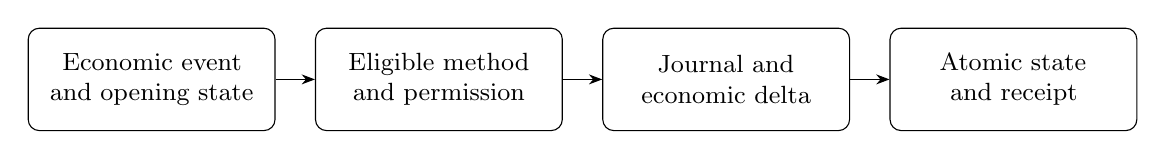
\begin{tikzpicture}[node distance=5mm,>=Stealth,
 box/.style={draw,rounded corners,align=center,text width=29mm,minimum height=13mm,font=\small}]
\node[box] (basis) {Economic event\\and opening state};
\node[box,right=of basis] (auth) {Eligible method\\and permission};
\node[box,right=of auth] (proposal) {Journal and\\economic delta};
\node[box,right=of proposal] (commit) {Atomic state\\and receipt};
\draw[->] (basis)--(auth);
\draw[->] (auth)--(proposal);
\draw[->] (proposal)--(commit);
\end{tikzpicture}
\caption{Each step answers a different question. Accounting assessment may
inform the permission decision, but only the final transaction changes the book.}
\end{figure}

For a delivery, the basis identifies the exact performance obligation,
quantity, allocation and control finding. The opening state contains cumulative
revenue, billing, collection and inventory. The selected method derives the
recognition and lot movements; the report later consumes that same committed
path. Combining a journal from one method version with a delta or opening state
from another is invalid even if the totals happen to balance.

\section{A lost acknowledgement must not create a second sale}
\label{sec:replay}

Suppose a sale commits but the response is lost. The client knows the request,
but cannot tell whether the server committed it. Retrying under a new event ID
could duplicate revenue. Retrying the original request must instead return the
original immutable receipt.

The lookup key is
\[
  (\text{entity},\ \text{book},\ \text{branch},\ \text{business event}).
\]
Payload, event version, opening state and request settings belong to the complete
fingerprint, not this key. A renamed run or bumped event version cannot evade a
conflict. A separately commissioned hypothetical projection uses a new branch
namespace; reopening the same projection uses its existing one.

A correction of an already committed event is a new business event linked to
its predecessor and an admitted correction method, such as reversal and
replacement or a dated adjustment. It preserves the original receipt.
The accounting treatment must apply to the actual correction; absent treatment
authority leaves it unresolved rather than licensing a generic reversal.

Commit first validates input shape, closure, bindings and authorization in the
requested historical view. It then looks up the stable event key. An equal
fingerprint returns the old receipt with no additional commit; a different
fingerprint returns an event-identity conflict. Only an absent key proceeds to
the expected-state and generation comparison. This order is essential: after
a successful sale the current head has changed, so checking freshness before
replay would reject the very retry needed to resolve the lost response.

A new candidate is assessed and constructed without mutation. One transaction
then rechecks key absence and the expected head, inserts journal, delta, closing
state, dependencies and receipt, and advances the head. It commits all or none.
If another client has committed the identical event, return that receipt. A
different event that advanced the head makes this request stale. A changed
payload under the same key conflicts. Diagnostic or scratch records never count
as economic transitions.

A timeout consequently has three possible observations: committed, not committed
or unknown. Unknown retains the original key, fingerprint and expected head for
receipt lookup or exact retry. Refreshing the head changes the request and cannot
be presented as the same retry. Missing committed dependencies are an integrity
failure, not permission to reconstruct an approximately similar receipt.

\section{Funding, tax and other simultaneous relations}

Some financial models have circular dependencies. Interest affects taxable
profit; tax and investment affect funding needs; funding affects interest.
The reference executor first tries to resolve these through explicit timing.
For example, beginning-of-period debt can determine current interest, with
new borrowing affecting the next accrual period. That is acceptable only when
the model's timing assumption is stated and appropriate.

Where the economic model genuinely requires simultaneous decisions, the
dependency graph identifies the strongly connected component and delegates it
to a declared equation or optimisation solver. The solver must return a
solution, residuals, admissibility checks and uniqueness or multiplicity
status. A contraction iteration requires a justified convergence condition;
an arbitrary fixed iteration count is not a mathematical solution. Multiple
admissible equilibria become alternatives when material. No solution produces
a model outcome such as financing failure, or an explicit numerical failure,
depending on the cause.

Funding policy must include available facilities, limits, covenants, collateral
and allowed capital actions. The program cannot issue unlimited debt to keep
cash positive. An inability to meet payments may be a legitimate default
outcome. Default ends or changes contractual and accounting processes under
the relevant event rules; it is not quietly discarded as a bad simulation draw.

\section{Worked example: identical history, different future journals}

Return to the company in Chapter~\ref{ch:purpose}. Immediately after the
historical interest payment and closing, cash is 95, debt is 100 and equity
is $-5$. There are no other assets, liabilities or transactions. Next year's
expense is 5 in the all-fixed branch and 7 in the all-floating branch under
the rate shock. The generated entries and closing statements are:

\begin{center}
\begin{tabular}{lrr}
\toprule Output & All fixed & All floating\\\midrule
Debit interest expense / credit cash &5&7\\
Closing cash &90&88\\
Closing debt &100&100\\
Current-year profit & $-5$ & $-7$\\
Closing equity after profit transfer &$-10$&$-12$\\
Cash change &$-5$&$-7$\\\bottomrule
\end{tabular}
\end{center}
The balance-sheet identity holds in each branch: $90=100-10$ and
$88=100-12$. The demonstration reporting profile classifies interest paid as
operating cash flow. A different permitted reporting profile changes that
classification, while preserving the cash movement and source event. This
example proves the intended distinction and its arithmetic; it does not
estimate the probability that either debt structure describes a real company.

\section{Worked example: a bond has several relevant amounts}

A two-period zero-coupon bond raises cash of 100 and promises 110.25 at maturity.
Assume a 5\% effective rate per period, no transaction costs, no default, and
amortised-cost treatment under a demonstration rule. The effective-interest
schedule follows directly from $100(1.05)^2=110.25$:
\begin{center}
\begin{tabular}{lrrr}
\toprule Date & Opening liability & Interest accretion & Closing liability\\\midrule
Issue &0&0&100\\
End of period 1 &100&5&105\\
End of period 2, before payment &105&5.25&110.25\\
Redemption &110.25&0&0\\\bottomrule
\end{tabular}
\end{center}
Issuance debits cash and credits the liability by 100. Each accretion debits
interest expense and credits the liability. Redemption debits the liability
and credits cash by 110.25. Legal face amount, carrying amount and market
fair value remain separate fields. A market-rate shock may change fair value
without changing this contractual payment schedule or this demonstration
amortised-cost path.

Cash-flow reporting uses the actual payment event and its economic components;
the annual accretion is non-cash. The applicable reporting package decides how
to classify the maturity payment, rather than inferring it solely from the
liability debit. Fees, modifications, early redemption, embedded options,
hedges and foreign currency require additional event and measurement rules.

Ordinary equity issuance similarly separates cash, share quantity and legal
capital. Ten new shares at 12, with par value 1, produce cash of 120, share
capital of 10 and premium of 110 under a simple par-value profile. Shares
outstanding increase by ten units. Direct issuance costs of 3 reduce the
specified equity account and cash under the chosen illustrative treatment.
The accounting rule and the cost's eligibility must be explicit; this example
does not prescribe every jurisdiction's treatment.

\section{Reporting and explanations}

The reporting engine produces the balance sheet, income statement, comprehensive
income, cash-flow statement, changes in equity and note schedules when the
necessary modules are present. Each output carries its basis, perimeter,
period, scenario and interpretation. A comparative table cannot combine an
original prior-year figure and a restated current-year comparative without
displaying that choice.

An explanation is a dependency graph with typed edges: extracted from,
interpreted as, assumed by, constrained by, generated by, measured by,
posted by, aggregated into and supersedes. A cash-flow line must lead back
to payment events; a fair-value movement must lead back to valuation inputs;
a consolidated amount must show eliminations. A provenance path establishes
how a result was obtained. It does not by itself establish that the underlying
economic model is correct.

\section{The corporate reference package as operations}

The Northstar example defines a closed, reproducible corporate package rather
than a universal standard. Its events separate performance, invoicing and
settlement even where the example makes the first two simultaneous. Every
payload includes entity/book, currency, economic date, period, source or
assumption IDs and an information-view ID. Amounts are exact before the
declared posting quantisation. Quantities and money are checked separately.

\begin{longtable}{L{27mm}L{60mm}L{49mm}}
\toprule Event & Preconditions and state change & Posting\\\midrule\endhead
Deliver/invoice & Goods owned and available; control transferred; quantity
removed at selected cost; unconditional amount due added & Debit receivable,
credit revenue; debit cost of sales, credit inventory\\
Collect & Receipt no greater than selected unpaid receivable; reduce that
balance; excess must be separately classified & Debit cash, credit receivable\\
Receive goods & Accepted owned quantity at supported unit cost; create supplier
obligation and inventory lot & Debit inventory, credit payable\\
Pay supplier & Identified obligation and sufficient available cash; reduce
both & Debit payable, credit cash\\
Payroll & Service period and cash obligation evidenced or assumed & Debit
payroll expense, credit cash; accrual variant uses a payable\\
Acquire plant & Control obtained, cost known, in-service date/life/residual
recorded; add asset cohort & Debit plant cost, credit cash or payable\\
Depreciate & In-service asset with remaining depreciable amount; apply dated
schedule, capped by that amount & Debit depreciation, credit accumulated
depreciation\\
Interest & Contract, reset state and accrual fraction known; create interest
obligation, then settle if cash available & Debit interest, credit interest
payable; debit payable, credit cash\\
Current tax & Reference tax base positive; 20\% teaching rule; apply prepaid
tax before further payment & Debit tax expense; credit prepaid tax or payable;
settlement separately affects cash\\
Dividend & Explicit authorised distribution, sufficient funds and permitted
capital action & Debit retained earnings, credit dividend payable; then settle\\
Close & Required period operations completed; preserve original movements &
Transfer temporary income/expense balances to retained earnings\\\bottomrule
\end{longtable}

The current example combines accrual and settlement when they share a date,
but the separate obligation remains the general operation. Customer advances
are debit cash/credit contract liability and become revenue only on the
supported performance event. Inventory costing requires an admissible policy;
negative inventory and collection beyond an identified claim are rejected.
Non-cash acquisitions, write-offs, impairment and currency movements require
their own classified templates. An unknown residual never enters one of these
operations merely to force a reconciliation.

Reporting maps asset and contra-asset balances into the balance sheet and
liability/equity balances with their opposite sign. Before closing, current
profit is included once in equity; after closing it is already in retained
earnings. Income uses period movements in income/expense accounts, and OCI
uses its own designated accounts. Cash flow sums cash legs by economic
operation: Northstar's collections, suppliers, payroll, interest and taxes
are operating, plant payments investing, and debt/equity proceeds or repayments
and dividends financing. Non-cash depreciation is excluded from direct cash
flow and added back only in the indirect reconciliation. Note schedules use
the same contracts, lots and classified movements as the statements.

\section{Scenario meaning and information access}

An \code{ExogenousStress} supplies a path or joint driver law while holding the
historical evidence model fixed. \code{ObservationalConditioning} additionally
supplies actual observations and a joint probability model; the finite method
in Chapter~\ref{ch:math} evaluates the conditional distribution when its
normalising mass is positive. \code{StructuralIntervention} requires a named
structural model and replaces designated equations, retaining its exogenous
noise. An absent structural model gives \code{UnsupportedScenario}, not an
intervention inferred from an accounting identity \citep[Section 3.2.1]{pearl2009}.
The textual Core 0 \code{scenario} declaration is an exogenous stress only;
the other modes require the explicit typed API records.

At each decision date the runtime constructs an information view containing
eligible disclosures, committed state through that date, currently observed
drivers and the declared forecasting model. Future realised innovations and
future outcomes are inaccessible. A stress path may be announced in advance,
but this is an explicit visibility policy. Otherwise management sees only its
current and past values. A bank's allowance at the opening date may use a
forecast distribution of defaults; it must not inspect the outer simulation's
future realised default. Inner valuation randomness has a separate stream
domain from outer realised outcomes.

Funding follows a declared waterfall: available cash, committed eligible
facilities up to their limits, and separately authorised capital actions.
Each action checks collateral, covenants and settlement timing. If an amount
remains due, record an economic funding failure and the unpaid obligation.
If required valuation or accounting is unsupported, stop the affected
dependencies as incomplete. The branch manifest preserves the last committed
state, completed outputs, unavailable outputs and reason. These distinctions
let an analyst see a meaningful bad outcome without confusing it with broken
computation.

\chapter{Accounting methods for an operating company}
\label{ch:modules}

\section{A common core with distinct accounting books}

The common core governs evidence, time, money, events, journals and provenance.
Reporting standards govern recognition, measurement and presentation within
that core. The design preserves three levels of meaning: economic terms such
as a promise to pay cash; an accounting treatment under a particular standard;
and a company's reported label or extension. These levels are connected by
explicit rules and mappings, rather than collapsed into one universal chart
of accounts.

A rule package includes a standards register with jurisdiction, issuer class,
effective dates, transition provisions, permitted elections, paragraph
references, implementation version and tests. The package selector uses the
entity, reporting basis, period and adopted elections. It must distinguish a
standard's mandatory effective date from permitted early adoption. For example,
the IFRS Foundation's IFRS 18 overview states an effective date of 1 January
2027 with earlier application permitted \citep{ifrs18}. A 2026 historical
report cannot be assigned that presentation regime solely because the latest
installed package includes it.

IFRS, US GAAP and ASBE packages share economic contracts and events where
appropriate, but produce separate accounting books. A reconciliation between
books consists of explained adjustments with origins in differing treatments,
not a renaming of accounts. The first implementation can preserve all three
source bases even while only a selected subset has executable rules. Such a
source is represented as observed information with unsupported simulation
treatments, rather than being silently converted to the supported basis.

The official IFRS overviews for IFRS 9, IAS 32 and IFRS 17 establish the relevant
scope of financial-instrument measurement, presentation and insurance
contracts \citep{ifrs9,ias32,ifrs17}. They are orientation sources, not substitutes
for reviewed paragraph-level implementations. The retained official Ministry of Finance ASBE~21 page now supports selected
lease provisions. The official 2017 ASBE~22 text also supports the selected
credit-loss, interest and write-off distinctions worked through in
Chapter~\ref{ch:banking} \citep{mofasbe22}. Entity-specific issuance and amendment
chains and broader ASBE authority remain incomplete. Chapter~\ref{ch:insurance}
compares the dated ASBE~25 premium-allocation and incurred-claim provisions
with the retained AASB~17 text \citep{mofasbe25}. The Ministry's 2025
explanation supports the stated entity-class timetable, while Ping An's
reports supply an actual adoption and comparative-restatement example
(Section~\ref{sec:insurance-adoption}). Direct verification of the operative
issuance and implementation notices remains open, including the detailed
conditions of the later simplifications. Current ASC access is also unresolved.
Historical amendments and issuer policies inform proposed comparisons without
substituting for operative authority. These source limits are addressed
explicitly in the following dated-method discussion.

\section{Non-financial companies}

The initial industry package covers sales, collections, purchases, payments,
inventory movements, payroll, capital expenditure, depreciation and basic
financing. Revenue recognition is a separate rule from invoicing and cash
collection. A service contract may generate a performance event before an
invoice, creating a different asset from an unconditional receivable. Customer
advances create obligations before revenue. Returns, rebates and variable
consideration need separate assumptions and subsequent adjustments.

Inventory state includes quantity, cost, location, ownership and lot or cohort.
A costing method is selected within the reporting package's permissible
domain. An aggregate stock can support a simple model only if its approximation
is declared. A commodity-price shock can expose differences between old and
new inventory that an average value suppresses. Fixed-asset state likewise
requires acquisition dates, components, useful lives, residual values,
depreciation method, tax basis and impairment history when those affect the
requested forecast.

Industry extensions add economic mechanisms without bypassing the accounting
core. Construction requires performance and completion states; extractive
industries require reserves, depletion and restoration obligations; utilities
may require rate-regulation treatment; software businesses may require
contract liabilities and development-cost decisions. The module manifest
states what is represented, what is executable, and what remains aggregated.

\section{A matched inventory case across reporting profiles}

Standards packages need operation-level decisions. For interchangeable goods,
the inspected AASB~102 text incorporating IAS~2 permits FIFO or weighted
average in paragraph 25 and explains both in paragraph 27
\citep{aasb102}. The reproduced ASBE~1 text specifies FIFO, weighted average
or specific identification in Article 14; its official Ministry version could
not be retrieved in this review, so that reproduction has provisional source
status \citep{asbe1copy}. Caterpillar's company-authored 2024 report states
that it principally uses LIFO and supplies a FIFO comparison
\citep[Note 1.C]{caterpillar2024}. That is evidence of a disclosed US-GAAP
company policy; full ASC~330 paragraph authority remains an acquisition task.
It is not a rule that every US company must use LIFO.

Take the same purchases in three separate books: ten units at 5, followed by
ten at 7, then delivery of twelve units. FIFO charges $10(5)+2(7)=64$ to
cost of sales and leaves inventory 56. LIFO charges $10(7)+2(5)=80$ and
leaves inventory 40. Periodic weighted average uses cost $120/20=6$, charges
72 and leaves 48. The physical deliveries and supplier cash flows agree;
profit and carrying inventory differ by the selected costing rule. A concept
mapping cannot remove that difference. The FIFO/average selector in an
IAS~2 profile rejects LIFO as an unsupported election under the inspected
paragraph. The US company profile admits its evidenced LIFO policy while
retaining its narrower authority. An ASBE package remains source-provisional
until the attributed text and applicable amendments are officially verified.

Inventory impairment illustrates another required memory. Under inspected
AASB~102 paragraphs 28--34, an item costing 56 written down to net realisable
value 50 records expense 6. If the conditions reverse and net realisable
value becomes 54, reversal is 4, capped by original cost; the previous
write-down must therefore remain in state. The reproduced ASBE~1 Article 19
also addresses reversal within the earlier provision. This paragraph is not
used to assert the US treatment, whose primary authority was unavailable.
Source limitations constrain the treatment claim, while the separate-book
method and exact costing calculations remain fully specified.

\hypertarget{operating-events}{%
\section{Operating events}\label{method-corporate-methods-operating-events}}

The operating methods use the selected revenue, inventory and asset provisions of \citet{aasb15dated,aasb102,aasb116dated}. The lease and gross-tax case uses the dated lease, income-tax and cash-flow compilations \citep{aasb16dated,aasb112dated,aasb107dated}. Each rule still needs the entity, period, transaction facts and elections described below.

Every event uses the event-basis, authorization and commit contracts described in Section~\ref{sec:posting-permission}. The event inputs described here are required in addition to identity and date. Each object identifier resolves to its contract, context and admitted source or assumption. A purported cash collection does not establish a sale; a purchase order does not establish receipt.


Revenue, billing and collection are separate transitions. A delivery event names
the contract, performance obligation, quantity, allocated price and control
evidence. Recognition first releases a related contract liability; earned
consideration not yet unconditional creates a contract asset. Both credit
revenue. A missing control finding or unresolved price constraint leaves the
recognition unresolved.

An invoice or right-to-payment event names the contract, bill and unconditional
amount. It debits the receivable and credits an existing contract asset, with
any excess recorded as a contract liability. A collection names that receivable,
settlement and amount and debits cash while crediting the receivable. An excess
payment needs a separate customer-advance method; it cannot be credited to
revenue merely because cash arrived. These transitions retain cumulative
performance, billing and collection independently.

Purchasing starts when the company receives owned goods, not when it places an
order. The event records lot, quantity, unit cost and ownership evidence, debits
inventory and credits the payable. Consigned or unreceived goods cannot pass
that ownership condition. Consumption or sale identifies an available lot
allocation, quantity and admitted cost formula; it debits cost of goods sold
or an eligible production asset and credits inventory. Overselling does not
create stock. Supplier payment separately debits the payable and credits actual
cash. Insufficient cash blocks that settlement and can trigger a separately
modelled default; it never creates a hidden loan.

A tangible-asset event records component cost, residual value, useful life,
depreciation method and the date it becomes available for use. Initial debit to
PPE has a corresponding cash or payable credit; depreciation later debits
expense or an eligible asset and credits accumulated depreciation. Employee
service records earned pay, deductions and employer obligations for the service
period, separately from settlement. Unknown labour or tax law cannot become a
zero payable.

Closing derives revenue, expenses, OCI and owner movements from those events
using admitted statement mappings. It checks cash, inventory, financing and tax
roll-forwards rather than introducing a balancing entry. These event fields
form the method's required inputs; each identifier resolves to the same
contract, context and evidence used by its authorization.


AASB 15 paragraphs 9, 22, 31, 35--43, 47--59, 73--86 and 105--108 provide the selected revenue conditions; the retained compilation dated 31 December 2022 applies to annual periods beginning on or after 1 January 2023 and before 1 July 2026, covering the stated for-profit FY 2024 example. Variable consideration is estimated under a selected method and admitted only subject to the significant-reversal constraint, not recognized solely because its unconstrained expectation is positive. Principal versus agent, returns, warranties, contract modifications and distinct bundles require their own scoped decision records. If their facts are unresolved, retain alternative eligible methods; do not borrow the simple delivery rule by label.

The following schedules make the distinction between performance and billing explicit. For one performance obligation with price 100, cumulative revenue 60, unconditional bills 50 and collection 30, AR=20, CA=10, CL=0 and cash=30. Revenue 60 is represented by those three assets. Billing before performance changes intermediate balances but not the final result. For bills 80 instead, AR=50, CA=0, CL=20; net assets remain 60. Cumulative performed-service cost 40 then 70 posts 40 then 30, not 110. A downward revision follows the correction method and keeps the old result tied to its original view.

For this simple contract, let $R$ be cumulative recognised revenue, $B$
unconditional billings and $C$ collections, with $0\leq C\leq B$. The unpaid
bills determine accounts receivable (AR); performance in excess of billing is
a contract asset (CA), while billing in excess of performance is a contract
liability (CL). After each event,
\[
 \mathrm{AR}=B-C,\quad \mathrm{CA}=\max(R-B,0),\quad
 \mathrm{CL}=\max(B-R,0),\quad \text{cash received}=C.
\]
This recurrence applies per contract, with no impairment, variable consideration or unbilled prepayment; it is not permission to offset unrelated contracts. For billing 80 before delivery, debit AR 80/credit CL 80. Recognizing service 60 later debits CL 60 and credits revenue 60. Collecting 30 debits cash 30/credits AR 30, leaving AR 50 and CL 20, without a second receivable or an artificial contract asset. If service comes first, recognize CA 60/revenue 60, then bill AR 80 against CA 60 and CL 20. Both orders end at the same state. Cash received before an unconditional bill needs an explicit advance event that debits cash and credits CL and records the advance applied to later billing; it cannot pass through collect(AR).

\subsection{A payment before the bill must be applied only once}
\label{sec:customer-advance}

The preceding recurrence deliberately excludes an advance before billing.
Suppose a customer pays 30 towards a service priced at 100. No service has yet
been performed and no payment was already due. The company now has cash 30 and
an obligation to provide the service, so it debits cash and credits a contract
liability. Crediting revenue would balance the entry but recognise performance
that has not occurred. Paragraphs 105--108 of the retained AASB 15 distinguish
this payment from an unconditional receivable \citep{aasb15dated}.

Now let the company earn 60 before issuing a bill. Recognition releases the
liability of 30 and creates a contract asset of 30, with a credit to revenue
of 60. The later invoice shows a gross amount of 80 and applies the customer's
advance of 30, leaving a new unconditional right to 50. Its entry debits the
receivable by 50, credits the contract asset by 30 and credits a contract
liability by 20. Creating a receivable of 80 would count the prepaid 30 again.
When the customer pays another 20, cash is 50, the receivable is 30 and the
contract liability is 20. Their net contribution to assets is the earned 60.

The method therefore keeps the invoice's gross amount separate from the right
still owed. Let $G$ be cumulative gross billings, $A$ cash advances, $K$ the
amount of those advances applied to bills, and $C$ later collections of
receivables. Each application names both its advance and its invoice; the
remaining unapplied credit is $A-K$. As before, $R$ is cumulative earned
revenue. The consideration already paid or made unconditionally due, counted
once, is $T=G+A-K$. For this one fixed-price contract,
\[
 \mathrm{AR}=G-K-C,\qquad
 \mathrm{CA}=\max(R-T,0),\qquad
 \mathrm{CL}=\max(T-R,0),\qquad
 \text{cash received}=A+C.
\]
The minus $K$ prevents the applied advance from appearing both in the cash
payment and in the bill. Since $\mathrm{CA}-\mathrm{CL}=R-T$, the control
\[
 (A+C)+(G-K-C)+\mathrm{CA}-\mathrm{CL}
 =G+A-K+R-T=R
\]
recovers the earned amount. This derivation uses a single contract, with
$0\leq K\leq\min(A,G)$, $0\leq C\leq G-K$ and $0\leq R,T\leq100$.
It provides no authority to offset different contracts or to ignore impairment,
financing, tax, cancellation or refund terms.

Each event must carry its contract, identity, date, currency and admitted
facts. In this restricted extension, advances precede all performance and
billing; later payments settle identified receivables. A revenue increment
first releases an existing contract liability and then creates a contract asset.
For a new gross bill $g$ that applies unused advance credit $k$, only $g-k$
creates a receivable. That amount releases the existing contract asset first;
any remainder increases the contract liability. The invoice consumes its
identified credit even if the advance has already been earned. A duplicate
credit application, an overcollection or missing unconditional-right evidence
cannot pass by adjusting a balancing account.

Billing before performance gives the same final balances in the example but
a different intermediate history. The invoice creates a receivable of 50 and
adds 50 to the existing contract liability of 30; earning 60 then releases 60
of that liability. After the later collection of 20, both paths have the
balances above. Completing the service adds revenue 40, releasing the remaining
liability of 20 and creating a contract asset of 20. A final bill for 20 and
collection of the remaining 50 leave cash 100 and no contract or receivable
balance. The actual sequence is retained even where endpoint amounts agree.

A wholly prepaid invoice exposes another implementation requirement. If its
gross amount and applied advance are both 30, it creates no new monetary right
and needs no accounting lines. It still consumes an identified credit. The
proposed authored method therefore declares a state-only journal proposal:
empty lines, zero account changes and explicit changes to the invoice and
advance allocations. Authorization checks that the net new right is zero;
the same atomic commit and replay rules protect the allocation from reuse.
An empty journal cannot carry a nonzero monetary effect. The native acquisition
schema requires nonempty lines and does not implement this case; an unavailable
authored schema returns an unsupported-operation result without changing state.

\input{sections/state-only-allocation}

These are revenue and cash contributions before service costs and tax. Their
missing measurements remain inputs to the complete company statements. The
next example retains a different obligation: cash already received may have
to be returned even after the goods have been delivered.

\subsection{A return right survives the sale}
\label{sec:customer-returns}

Consider 100 goods sold for 10 each, with a former inventory cost of 6 each.
The buyer obtains control, pays cash and has a contractual right to a refund
for returned non-defective goods. Assume an eligible Australian for-profit
contract in 2024, within the retained AASB 15 compilation's application period.
The contract, control, price-estimation and significant-reversal conditions
are separately satisfied; immediate cash receipt alone would not establish
them. The numbers are synthetic measurements, not estimates of Apple's returns.

If the company initially expects 10 goods to be returned, it expects to retain
900 of the 1,000 received. AASB 15 B20--B25 requires revenue for the expected
entitlement, a refund liability and a separate asset for the right to recover
the goods \citep{aasb15dated}. With no expected recovery costs or deterioration
in this example, the refund liability is 100 and the recovery asset is 60.
The company debits cash 1,000, credits revenue 900 and credits the refund
liability 100. It removes inventory 600 by debiting cost of sales 540 and the
recovery asset 60. Pretax profit is therefore 360. Recognising the full 1,000
as revenue would omit a known refund obligation, although the entry balances.

For a homogeneous cohort of $N$ units, unit price $p$, former unit cost $c$ and
an admitted estimate $q$ of returns, the initial no-recovery-cost case gives
\begin{align*}
 \text{revenue}&=(N-q)p, & \text{refund liability}&=qp,\\
 \text{cost of sales}&=(N-q)c, & \text{recovery asset}&=qc.
\end{align*}
The estimate and its measurement date are retained with the cohort. Paragraphs
53--59 require an appropriate estimation method and the constraint on a
significant reversal; $q$ is not a probability supplied by the accounting
standard. Missing evidence for that measurement leaves the amount unresolved.
After actual returns begin, the state separately records refunded units,
remaining expected returns, remaining liability and recovery rights. A later
outcome cannot be inserted into the original information view.

Suppose the sale occurs in 2024 and new information at year end raises expected
returns to 12. The liability increases by 20, reducing revenue by 20. The
recovery asset increases by 12, reducing cost of sales by 12. Closing revenue
is 880, cost of sales 528 and pretax profit 352. The change in expectations
does not itself establish an error in the original estimate. If the opening
inventory of 600 was financed entirely by opening equity of 600, the resulting
pretax balance sheet has cash 1,000 and recovery asset 72, against refund
liability 120 and equity 952.

In 2025, assume the return period ends with eight accepted returns and no
remaining legal right or unresolved claim. Before final settlement, remeasure
the liability from 120 to 80 and the recovery asset from 72 to 48. The first
change credits revenue by 40; the second debits cost of sales by 24. Refunding
80 then debits the liability and credits cash. Receiving the eight goods
debits inventory by 48 and credits the recovery asset by 48. Settlement does
not recognise the sale or its cost a second time. The 2025 pretax profit
contribution is 16, closing cash is 920 and inventory is 48. With no other
movements, equity is 968: opening 600 plus cumulative profit 368.

The cash and accrual statements can now be checked independently. Operating
cash is 1,000 in 2024 and $-80$ in 2025. In the indirect method, the first
year adds the inventory reduction and liability increase to profit while
subtracting the recovery-asset increase. The second year reverses the relevant
balance movements:
\begin{align*}
 \mathrm{CFO}_{2024}&=352+600-72+120=1{,}000,\\
 \mathrm{CFO}_{2025}&=16-48+72-120=-80.
\end{align*}
There is no investing or financing cash flow, OCI or subsequent owner
transaction in this slice. Tax has not been computed: these pretax
contributions must enter the separate current/deferred-tax method before they
can become complete after-tax company statements.

Recovery costs change the asset without necessarily changing the refund. For
the 12-unit estimate, expected recovery costs of 1 per unit and deterioration
of 0.5 give a recovery asset of $12(6-1-0.5)=54$. Cost of sales becomes 546
and pretax profit 334, while the refund liability remains 120. The cost inputs
are measurements, not automatic zeros; estimating them does not pay cash early.
Paragraph B25 also requires separate presentation of the asset and liability.
Showing only their net 48 in the original no-cost case would conceal both
the gross right to recover goods and the gross obligation to refund cash.

Scope conditions matter as much as the arithmetic. Paragraph B26 treats an
exchange for the same type, quality, condition and price differently from a
return; B27 sends a defective-product replacement to warranty guidance.
The refund method cannot accept those events simply because the goods move
back to the seller. It also needs the contractual return window, accepted-unit
identities, actual refund and recovery measurements, and evidence that any
remaining rights have expired before clearing the balances. An unknown
estimate yields unresolved, absent control makes recognition ineligible, and
an event of a different kind remains outside this method. Inventory costing
and the condition of recovered goods continue to have their own requirements.

\subsection{A warranty can promise another year of service}
\label{sec:service-warranty}

A returned product and a warranty claim need different histories. The return
example unwinds a sale when a customer exercises a refund right. A warranty
may instead promise to keep a product working, or provide a service after the
product has been delivered. The company must identify which promise it made
before deciding how much of a customer's payment it has earned. The following
cases use the same retained AASB 15 compilation and historical Australian
for-profit scope as the return example.

Suppose a customer buys a product and a separately purchasable service warranty
for a combined 108. Comparable standalone selling prices at contract inception
are 100 for the product and 20 for the warranty. Both are distinct promises;
the product works independently of the additional service. The contract has
neither a discount attributable to just one promise nor variable consideration.
Under paragraphs 73--86, the 12 bundle discount is therefore allocated in
proportion to the standalone prices. The product receives
$108\times100/120=90$ and the service receives $108\times20/120=18$.
An invoice's labels would not by themselves establish those standalone prices
or justify a different discount allocation \citep{aasb15dated}.

On 1 July 2024 the company receives 108 and transfers control of the product,
whose inventory cost is 60. First, receipt debits cash and credits the contract
liability by 108. Delivery then debits that liability and credits product
revenue by 90, while debiting cost of sales and crediting inventory by 60.
Profit is 30 and a liability of 18 remains. Recognising all 108 on delivery
would credit revenue for service the company still owes.

The service warranty runs for twelve monthly service periods to 30 June 2025.
The company stands ready uniformly; the customer receives and consumes the
benefits as service is supplied. The admitted measure gives each completed
service month one twelfth of the allocation and faithfully depicts performance.
These facts support over-time recognition under
35(a), 39--45 and B14--B19; the existence of a twelve-month date range alone
would not suffice. At 31 December 2024, half the service has been provided,
so half of 18, or 9, is earned. Debit the contract liability and credit
service revenue by 9. Actual service costs of 3 are expensed and paid.
Opening inventory and equity were both 60, with no other opening balances.
Year-one revenue is now 99, expenses 63 and pretax profit 36. Cash 105 equals
the remaining liability 9 plus equity 96.

The second half-year releases the remaining liability of 9 and incurs another
3 of paid service costs. Its profit is 6 and closing cash and equity are both
102. Over the complete contract, revenue 108 less costs 66 gives profit 42.
The cash statement follows the same history: operating cash is 105 in the
first period and $-3$ in the second. The independent accrual bridges are
$36+60+9=105$ and $6-9=-3$, using the inventory reduction and changes in the
contract liability. There is no OCI or subsequent owner transaction in this
pretax slice; the complete company calculation still needs tax and any other
obligations.

The contract record must therefore retain the two promises, the original
allocation and its price evidence, delivery identity, coverage, progress
measure, cumulative service revenue and actual costs. Each service update
posts the difference between newly supported cumulative revenue and revenue
already recognised. Replaying an accepted delivery cannot release the product
allocation twice. Unknown progress is not zero performance: paragraphs 44--45
require a separate assessment of reasonable measurement and, where applicable,
cost recovery. This percentage method cannot invent those findings.

The classification also has a substantive boundary. A separately purchasable
warranty is a distinct service under B29. Without that option, B30 sends an
assurance-only warranty to AASB 137 unless it provides additional service.
Law, duration and promised tasks help distinguish the cases under B31; there
is no universal number of months that makes a warranty a service. If assurance
and additional service cannot reasonably be accounted for separately, B32
treats the two warranties together as one performance obligation. Harm or
infringement compensation under B33 is not such a service. The historical
AASB 137 population-measurement case in Section~\ref{sec:corporate-residuals}
supplies the separate assurance method. Actual coverage, claims, timing and
reimbursement evidence remain required; missing facts cannot become a zero
provision or convert assurance into this service example.

\subsection{Changed promises can affect future units or past progress}
\label{sec:customer-modification}

A contract can change after some performance has already been recognised.
The accounting consequence depends on what remains to be supplied. Consider
an original prepaid order for ten distinct units at 10 each. Four have been
delivered, earning 40. The parties approve an enforceable amendment adding
six units for 48. Comparable standalone prices remain 10 each, and no
appropriate contract-specific adjustment makes the 48 addition reflect
those prices. The addition therefore fails the separate-contract condition
in paragraph 20. Because the remaining units are distinct from those already
delivered, paragraph 21(a) reallocates the consideration for the remaining
performance \citep{aasb15dated}.

The undelivered original units carry 60 of consideration. Adding the new 48
gives 108 for twelve remaining units, whose standalone prices are equal.
Thus their new unit allocation is
\[
 \frac{\text{unrecognised original consideration}
       +\text{additional consideration}}
      {\text{remaining equal-price units}}
 =\frac{60+48}{6+6}=9.
\]
The first four units keep their revenue of 40. Spreading the entire revised
price over all sixteen units would instead give $148/16=9.25$ and rewrite
their revenue as 37. That calculation is wrong for the stated facts: this
modification reallocates remaining performance, not completed deliveries.

Inventory and cash make the consequences concrete. Start with sixteen units
costing 6 each, financed by opening equity of 96; six units were initially
uncommitted. The first prepayment debits cash and credits a contract liability
by 100. The first four deliveries release 40 of revenue and remove inventory
cost 24. Immediately before amendment, cash 100 plus inventory 72 equals the
liability 60 plus equity 112. Receipt of the additional 48 increases cash
and the liability. Approving the changed order itself earns no new revenue
and creates no new stock.

Deliver six more units by the first year end. They release liability and
revenue of 54, with inventory cost 36. Total year-one revenue is 94, cost
of sales 60 and profit 34. Cash 148 and inventory 36 equal liability 54
and equity 130. Delivering the final six in the next year earns another
54 at cost 36, leaving cash and equity 148 with no inventory or contract
liability. That period's profit is 18 but no cash arrives: the customer
already paid. The operating cash bridges are $34+60+54=148$ and
$18+36-54=0$. Lifetime revenue 148 less inventory cost 96 gives profit 52.

If the additional six units instead cost 60 and meet paragraph 20's
standalone-price condition, the addition is a separate contract. The first
four still earn 40; the six remaining original units earn 60 and the new
six earn 60. Both contracts keep their own allocation records. The difference
between these cases is the admitted price and scope assessment, not permission
to choose whichever result produces the preferred margin.

An integrated promise can have the opposite effect on past cumulative
revenue. Suppose a customer controls work in progress as the company creates
it, satisfying paragraph 35(b). The company has one integrated performance
obligation, and its remaining work is not distinct from work already supplied.
Original price 100 and supported output progress of 40\% yielded revenue 40.
An approved enforceable amendment changes that same promise to price 130;
the revised faithful output measure is 30\% of the expanded work. Under
21(b), both the price and progress change the cumulative amount earned:
\[
 \text{revised cumulative revenue}=130\times0.30=39,
 \qquad \text{catch-up}=39-40=-1.
\]
The new work makes the completed work a smaller share of the promise.
Revenue decreases by 1 at amendment even though the total contract price
increases. The old 40 remains attached to its original information view;
the modification does not establish that the earlier estimate was an error.

For a complete prepaid example, start with cash and equity 50. Receive 100
and pay service costs 30 before amendment. Recognition of 40 leaves cash
120, liability 60 and equity 60. At amendment, receive the additional 30
and debit revenue 1 while crediting the liability 1. Cash is now 150,
the liability is 91 and equity is 59: cumulative revenue 39 less costs 30
has earned profit 9. Operating cash since opening is 100, also $9+91$.
Completing the promise next period releases revenue 91 and incurs further
paid service costs of 60. Period profit is 31, operating cash is
$31-91=-60$, and closing cash and equity are 90. Lifetime profit is
$130-90=40$. The output progress percentages were independently supported;
they were not inferred from these cash costs.

Both modifications need the approved rights, effective date, previous and
revised promise, consideration, performance measurements and source versions.
The distinct-goods method freezes the fulfilled deliveries and replaces the
remaining allocation; the integrated method proposes only the difference
between revised cumulative revenue and the amount already recognised.
Economic state and journals change atomically. Different billing schedules
can require a contract-asset adjustment instead of the prepaid liability
entries used here. A request that has not been approved leaves the existing
contract operative under paragraph 18. Unknown enforceability stays
unresolved; approved scope with undetermined price requires paragraph 19's
variable-consideration estimate and constraint, not a price of zero.

Paragraph 21(c) also admits mixed remaining obligations, requiring an explicit
allocation consistent with the two principles above. The examples do not
force such a contract into one category. Price-estimate changes without a
contract modification follow 87--89. A later price change after modification
needs paragraph 90: variable consideration promised before a 21(a)
modification can still be allocated to the earlier obligations under 90(a).
It cannot automatically be spread over the twelve remaining units merely
because their current allocation is 9 each.

\subsection{The same cash can accompany different revenue}
\label{sec:principal-agent-cash}

Suppose an entity receives 120 from a customer and sends 100 to a supplier.
It keeps 20. Those cash movements cannot tell us whether it sold the supplier's
good or arranged a sale by that supplier. Under B34--B38, the decision starts
with the specified good or service and whether the entity controls it before
transfer to the customer. Responsibility for delivery, inventory risk and
price discretion inform that decision; none is a substitute for control, and
momentary legal title does not by itself establish it \citep{aasb15dated}.

In the principal case, the entity controls the identified good before
customer transfer, can direct its use and obtain its benefits, and is
responsible for delivering it. Acquisition on credit debits inventory 100
and credits the supplier payable 100. Customer transfer and cash receipt
debit cash 120 and credit revenue 120; the inventory leaves through cost
of sales 100. Settling the supplier debits the payable and credits cash 100.
From zero opening balances, the result is cash and equity 20, revenue 120
and profit 20.

In the agent case, the supplier controls the good until transfer; the entity
only arranges the sale and earns a fixed commission of 20 when that service
is completed. Assume the entity controls the collected cash and owes the
supplier 100 under its remittance agreement. Funds held outside its balance
sheet in a fiduciary capacity are outside this example. Receipt therefore
debits cash 120, credits the supplier payable 100 and credits commission
revenue 20. Settlement clears the payable against cash 100. The agent has
no inventory or supplier cost of sales. Its final cash, equity and profit
are again 20, but revenue is 20.

Even the intermediate balance sheets agree: before remittance, both have
cash 120, a payable 100 and equity 20. The different control facts explain
the different revenue. The method must retain those facts and classify each
specified promise separately, since the same entity can act as principal
for one promise and agent for another. An unknown control finding leaves
classification unresolved; the receipt cannot decide it. Both cash legs
remain in the ledger. Whether the cash-flow statement presents receipts and
remittances gross or net requires its own AASB 107 conditions, which do not
follow merely from the revenue classification. These examples establish
the cash change and pretax profit contribution while preserving that separate
presentation question.


\subsection{An idle factory does not make its remaining stock more valuable}
\label{sec:production-capacity-cost}

Producing fewer goods leaves the factory's fixed costs spread over fewer
units, but that arithmetic does not establish their inventory cost. Consider
a factory that normally makes 100 good units each year after allowing for
planned maintenance. Its annual fixed production overhead is 180. If it
makes only 60 units, dividing all 180 by 60 would assign 3 to each unit,
rather than the normal 1.8. The unsold goods would then carry part of the
cost of idle capacity into the next year.

AASB 102.13 prevents that result. Fixed production overhead is allocated
using normal capacity; low output does not increase the amount per unit,
and unallocated overhead is expensed. Abnormally high output requires a
lower allocation per unit so that inventory is not measured above cost
\citep{aasb102compiled2021}. Normal capacity is an estimate of average
production under normal conditions, including planned maintenance. It
requires evidence separate from the actual output or desired margin.

Use a synthetic manufacturer in calendar 2024 and the retained AASB 102
compilation dated 31 December 2021. Its documented application interval
includes that year; subsequent amendment and actual-entity admission remain
separate. The company makes one ordinary manufactured product, with no
opening stock, work in progress, joint products or normal production loss.
One material kit produces one good unit. A kit costs 2; direct labor costs
1 and variable production overhead costs 1 per good unit, all paid in cash.
These goods are outside the agricultural, financial-instrument and
broker-trader exceptions. Periodic weighted average is used for this
homogeneous batch under paragraphs 25--27.

The fixed 180 consists of cash factory management and maintenance of 120
and depreciation of 60. Opening factory PPE is 600, with ten remaining
years, zero residual value and admitted uniform time-based consumption.
There is one component and recoverability has been separately established.
The depreciation method therefore remains unchanged across the output
scenarios. Paragraph 12 includes factory depreciation and production
administration among production overheads; AASB 116.48--49 allows
depreciation to enter another asset's carrying amount when appropriate
\citep{aasb116dated}. Recording it in inventory does not make it a second
cash payment.

Keep excluded costs visible. A separately documented accident destroys six
unused kits costing 12 before labor or conversion. They are additional to
the kits used for good output and have no salvage value. Unrelated
head-office administration of 10 and period selling services of 8 are also
paid in cash. The abnormal loss and these unrelated expenses do not bring
the good units to their present location and condition, so paragraphs
10--16 exclude them from inventory. Factory management and head-office
administration cannot be classified solely from the word \emph{administration}.

All completed goods have supported net realisable value of 10 per unit,
with no further completion or sale costs. The example therefore still
applies the lower-of-cost-and-NRV requirement rather than suspending it.
Delivered units sell for cash of 10 each under an approved, enforceable
single-product contract: rights and payment terms are identified,
collection is probable, the contract has commercial substance, and
delivery, acceptance, title and control transfer coincide. There are no
remaining promises, returns or concessions. These facts admit the
existing AASB 15.9 and 31--38 delivery method \citep{aasb15dated}; cash
receipt by itself would not do so.

\subsubsection{Allocate the cost that production can carry}

Let \(Q\) denote good completed units and \(S\) the units sold, with
\(0\leq S\leq Q\). For this single cost pool, normal capacity is 100
and fixed overhead is 180. Each good unit first receives its direct and
variable cost of \(2+1+1=4\). When output is low, the fixed allocation
is 1.8 per unit; when output is abnormally high, the total allocation is
capped at the 180 actually incurred. For \(Q>0\), this gives
\[
 f(Q)=\frac{180}{\max(100,Q)},\qquad
 u(Q)=4+f(Q),\qquad
 U(Q)=180-Qf(Q),
\]
where \(f\) is fixed overhead per unit, \(u\) is admitted unit cost
and \(U\) is unallocated overhead expensed now. This compact formula
implements the stated homogeneous, constant-cost example. Multi-product
pools, work in progress or changed production resources require their own
allocation. With no output, there is no unit cost to divide by: stock is
zero and all 180 is current expense.

At low output \(Q=60\), the good units carry fixed overhead of
\(60\times1.8=108\), leaving 72 as current expense. Unit cost is 5.8.
Selling 40 units removes inventory cost 232; the other 20 remain at 116.
Abnormal waste 12 and the unrelated administration/selling cost 18 are
also current expenses. Revenue 400 therefore leaves pretax profit
\(400-232-72-12-18=66\). Normal output of 100 absorbs all 180 at
the same unit cost of 5.8. Abnormally high output of 150 instead allocates
\(180/150=1.2\) per unit, giving unit cost 5.2.

The comparison below changes output and sales explicitly. All arms retain
the same fixed costs and the separately stated accident. They do not have
equal total production spending: direct and variable costs change with
good output. Sold-stock cost means the carrying amount removed on sale;
AASB 102.38 also includes unallocated overhead and abnormal production
costs in the broader inventory expense.

\begin{center}
\small
\begin{tabular}{lrrrr}
\toprule
& Low & Normal & High & Idle\\
\midrule
Good units / sold units & 60 / 40 & 100 / 80 & 150 / 120 & 0 / 0\\
Unit cost & 5.8 & 5.8 & 5.2 & n/a\\
Unallocated fixed expense & 72 & 0 & 0 & 180\\
Sold-stock cost & 232 & 464 & 624 & 0\\
Closing inventory & 116 & 116 & 156 & 0\\
Broader inventory expense & 316 & 476 & 636 & 192\\
Pretax profit & 66 & 306 & 546 & $-210$\\
Closing cash & 1010 & 1250 & 1450 & 850\\
Closing PPE & 540 & 540 & 540 & 540\\
Pretax net assets & 1666 & 1906 & 2146 & 1390\\
\bottomrule
\end{tabular}
\end{center}

Opening cash is 1000 and PPE is 600, so opening net assets are 1600.
There are no payables, borrowing or owner movements in this slice. Tax
effects are uncomputed: the last row is a pretax net-assets reconciliation,
not after-tax equity, distributable profit or a complete statutory set of
statements. This boundary avoids manufacturing tax law to finish the
example. Each arm has separately reconciled cash, stock and PPE; an
after-tax extension must supply the relevant tax bases, rates and timing.

\subsubsection{Preserve both the cost origin and the cash movement}

The low-output journal path starts with 66 kits costing 132. Debit raw
materials and credit cash 132. The accident debits abnormal-loss expense
12 and credits raw materials 12. Transferring the 60 good kits to
production moves raw-material cost 120 into finished goods; direct labor
60 and variable overhead 60 enter the same goods account against cash.
No raw materials remain, and the goods initially carry 240.

The fixed costs first enter a production clearing account: debit it 120
against cash and 60 against accumulated depreciation. Then debit
finished goods 108 and unallocated-overhead expense 72, crediting the
clearing account 180. Its balance is now zero, and finished goods cost
348. The separate administration and selling entry debits expense 18
against cash. On delivery, debit cash and credit revenue 400, then debit
sold-stock expense and credit finished goods 232. The final 116 is the
cost of 20 unsold goods, not a residual chosen to make the books balance.

Cash receipts of 400 less payments of \(132+60+60+120+18=390\)
increase cash by 10. The whole factory's depreciation is 60 even though
part remains in inventory. To reconcile pretax profit with operating cash,
add that noncash consumption and subtract the full inventory increase:
\[
 \Delta\mathrm{cash}=66+60-116=10.
\]
The stock includes depreciation of
\(20\times60/100=12\). An equivalent reconciliation adds only the
48 of depreciation reaching current profit, but then subtracts only the
cash-cost part of stock, \(116-12=104\): \(66+48-104=10\).
Adding back 48 while subtracting all 116 would wrongly report a cash
decrease of 2. The two valid methods differ in presentation, not in the
underlying cost population.

Selling all 60 good units in the low-output arm provides a second check.
Production and its payments are unchanged. Revenue becomes 600,
sold-stock expense 348, profit 150 and cash 1210; inventory becomes zero.
The additional 200 cash receipt releases inventory cost 116 and increases
profit by 84. Total pretax net assets become 1750. This is why a forecast
needs both production and sell-through, rather than an inventory margin
inferred from total factory spending.

\subsubsection{Balanced books can still defer the wrong costs}

If low output absorbed all fixed overhead using \(180/60=3\) per
unit, unit cost would be 7. Unsold stock would be 140 and profit 90,
each 24 above the admitted result; cash would remain 1010. The books
would balance, but they would postpone idle-capacity expense in the
remaining goods. At high output, applying 1.8 without a cap would allocate
270 of fixed cost when only 180 was incurred. Crediting a variance of 90
to balance that over-allocation would leave stock 174 and profit 564,
both overstated by 18. A balanced variance cannot create an incurred cost.

Capitalizing abnormal loss 12 and unrelated period costs 18 into the
60-unit batch would defer \(30\times20/60=10\) of excluded expense
in unsold stock. This is a separate classification error from the
capacity error. Each resource therefore retains a purpose and identity,
its membership in the cost pool, and its cash or noncash origin. The
state also retains capacity evidence, good and lost units, batch cost
and quantity, and the specific sale removals. A duplicate resource or
negative stock is invalid; a revised capacity estimate creates a new
supported allocation decision instead of overwriting an earlier result.

Unknown normal capacity leaves the fixed allocation unresolved. Unknown
NRV prevents a complete closing measurement, and missing control-transfer
facts prevent revenue recognition. Work in progress, joint products and
heterogeneous cost populations require a different specified model rather
than silent use of this unit formula. The proposed procedure and checked
case define those boundaries; they do not establish production-engine
conformance or an actual manufacturer's accounting treatment.


\hypertarget{sec:corporate-residuals}{%
\subsection{Changed obligations and unfinished production}\label{sec:corporate-residuals}}

A company can change its restoration estimate before a machine wears out, promise to repair sold products, or end a period with unfinished goods. Each condition changes a different part of its accounts. The following cases extend the preceding operating methods through those transitions. They retain exact illustrative amounts and separate economic evidence from bookkeeping.

Restoration, production and uncertain-tax methods use the retained historical EU text; assurance and mixed contracts use the inspected AASB compilations for synthetic 2024/2025 Australian for-profit reporters. The AASB 137 PDF covers annual periods beginning from 1 January 2023 to before 1 July 2026; its website gives a different end-period summary. Both admit these particular historical calendar years. A real application still needs its own source and period admission. Amounts are pretax unless an explicit tax calculation follows.

\hypertarget{restoration-estimates-change-the-asset-and-the-obligation-differently}{%
\subsubsection{Restoration estimates change the asset and the obligation differently}\label{restoration-estimates-change-the-asset-and-the-obligation-differently}}

The restoration record retains the related component and liability, cost/revaluation policy, gross cost/accumulated depreciation, remaining life/residual, current cash-flow estimate and rate, prior estimate identity, same-asset revaluation surplus/prior profit deficit, hypothetical cost-model carrying amount, impairment evidence and whole-class valuation review. IFRIC~1.2 \citep[IFRIC~1.1--8]{eu20231803} requires the original liability to have been included in the asset's cost. A standalone litigation obligation is not admitted to this asset-adjustment method.

Separate passage of time from a new estimate. Under the cost model, a liability increase adds to PPE; a decrease reduces PPE only to zero, with excess in profit. An increase prompts assessment of impairment indications and an IAS 36 test when required. Depreciate the adjusted carrying amount less admitted residual over the remaining useful life. Discount unwind is finance expense, never capitalised under IFRIC 1.8. Once useful life is exhausted, later estimate changes go to profit under 7 regardless of asset model. Actual settlement reduces the obligation and cash; a difference from the last carrying amount requires a dated remeasurement.

With cash 100, PPE 80 and provision 20, opening equity is 160. An admitted new provision 50 adds 30 to PPE. Recoverable amount 90 requires impairment 20: PPE 90, cash 100, liability 50 and equity 140. Four years remaining and zero residual gives annual depreciation 22.5. The subsequent depreciation-only illustration assumes a separately supplied zero discount rate and no further liability change; PPE 67.5 and equity 117.5 follow. In another branch, PPE 30/provision 80 and a new provision 30 require Dr provision 50 / Cr PPE 30 / Cr profit 20. Negative PPE 20 would be wrong. Cash 100 then equals liability 30 plus equity 70.

Under the revaluation model, a liability increase first consumes a same-asset surplus through OCI, then affects profit; a decrease reverses a same-asset profit deficit and otherwise increases OCI. A decrease exceeding the hypothetical cost-model carrying amount has an immediate profit component. Determine any necessary class revaluation first so that these splits use the correct history. With PPE 150/provision 50/surplus 20, an increase 35 gives OCI loss 20 and profit loss 15; PPE stays 150 only because a supplied class valuation review supports it. Cash 100 then gives equity 165 and liability 85. Surplus on another asset cannot be borrowed. In a separate decrease case, PPE 25, hypothetical cost 40, earlier profit deficit 15 and provision 80 → 30 yield excess 10 plus deficit reversal 15 in profit and 25 in OCI. Cash 100+PPE 25=provision 30+equity 95. Using 25 as the cost floor would compute the wrong split. The prior deficit explains why 25 and 40 differ; no fresh impairment is inferred from that difference.

A full cash history opens cash 100/PPE 120/provision 20/equity 200. Two-year straight-line life and zero residual give depreciation 60 in year 1. At 10\%, unwind 2 raises the provision 22; new supported estimate 33 adds 11 to PPE. Close PPE 71/provision 33/equity 138, with pretax loss 62 and no cash change. Year 2 depreciation 71 and unwind 3.3 give loss 74.3; actual settlement 36.3 leaves cash/equity 63.7 and zero PPE/provision. Across both years depreciation 131 plus finance 5.3 equals cumulative loss 136.3. The total cash bridge is exact; IAS 7 classification of restoration settlement needs a separate fact-specific policy. The method therefore returns a cash-classification obligation rather than inventing a complete categorized cash-flow statement. A fully exhausted PPE 0 with provision 20 → 25 gives expense 5 even if a historic revaluation reserve exists.

\hypertarget{assurance-is-a-measured-obligation-alongside-the-product-sale}{%
\subsubsection{Assurance is a measured obligation alongside the product sale}\label{assurance-is-a-measured-obligation-alongside-the-product-sale}}

The assurance record stores covered sales/population, legal or constructive promise, coverage/task findings, claim history, remaining-outcome law, timing/discount, reimbursement contract and virtual-certainty evidence. AASB 15.B 28--B 33 determines whether assurance, service or an inseparable combined service is present. AASB~137.14/24 \citep[paras.~14,24,36--62]{aasb137dated} admission precedes measurement. For a large population 39 uses weighted outcomes; individual claim probability does not replace the population outflow judgment. Correlation matters for distributions even when marginal means are sufficient to add expected cost. A single lawsuit uses 40's different analysis.

Consider 100 products with admitted per-product costs 0,10,40 and probabilities 3/4,1/5,1/20. The population estimate weights each possible repair cost and then sums across the covered products:

\[100\left(\frac34\,0+\frac15\,10+\frac1{20}\,40\right)=400.\]

A low claim probability for one product therefore does not eliminate the population obligation. The entire population has a present assurance duty, probable outflow and reliable estimate; discount is immaterial over the short horizon. Opening cash 1000 and inventory 600 are funded by equity 1600. Cash sales 2000 and inventory expense 600 accompany warranty expense/provision 400. An independently enforceable quarter-cost reimbursement is virtually certain on settlement, so recognise a separate asset 100/benefit 100. Do not net it against the provision. Paragraph 54 permits net expense presentation.

Pay claims 100 and receive reimbursement 25. A new remaining-claims estimate 250 replaces the old 300, releasing 50; reduce the remaining reimbursement 75 to 62.5, expense 12.5. Year 1 cash 2925+reimbursement 62.5=provision 250+pretax equity 2737.5. Profit 1137.5 follows from 2000 − 600 − 400+100+50 − 12.5. Direct operating cash 1925 also equals profit 1137.5+inventory release 600+provision increase 250 − receivable increase 62.5. Year 2 settlement 250 and receipt 62.5 leave cash/equity 2737.5 with no further profit under the realised amounts. Without virtual certainty, no reimbursement asset is recognised; retain the separate uncertainty. Missing claim evidence does not permit zero provision or the printed 400 by default.

\hypertarget{a-mixed-amendment-needs-two-revenue-calculations}{%
\subsubsection{A mixed amendment needs two revenue calculations}\label{a-mixed-amendment-needs-two-revenue-calculations}}

The modification record retains the original allocation/performance, enforceable change, remaining distinctness findings, amended allocations, faithful measures of progress and new receipts. AASB~15.21(c) \citep[paras.~18--21,39--45,73--90]{aasb15dated} requires consistent application of 21(a)/(b) to the affected promises; it does not supply a universal price split. The following exact case deliberately removes discount-allocation ambiguity.

A contract includes construction 100 and four distinct inspection visits 5 each, at their evidenced standalone prices. Inspections concern another operating line and can occur before the new construction finishes. The original expected construction cost 80; actual eligible cost 40 and faithful cost-to-cost progress give 50\% and revenue 50. One visit adds revenue 5 and cash expense 2. The 120 price was prepaid. The approved amendment adds integrated construction 40 and two visits 10; supported standalone allocations therefore become 140 and 30. New total construction cost 100 makes cumulative progress 40\%. The amended construction allocation gives
\[\text{cumulative revenue}=140\frac{40}{100}=56,\qquad\text{catch-up}=56-50=6.\]
This corrects only the construction promise. The first visit's 5 remains; five remaining distinct visits share 25 prospectively. The new 50 receipt itself earns no revenue.

With opening cash/equity 100, two additional visits by year-end yield revenue 71, expense 46, profit 25, cash 224 and contract liability 99. The indirect operating bridge 25+99=124 matches 170 received − 46 paid. Complete construction for cash 60 and three visits for 6 next year: revenue 84+15=99, profit 33 and cash/equity 158. Lifetime profit 58=price 170 − construction 100 − visit costs 12. Keeping old progress would recognise 70 for construction; applying 40\% to the entire 170 would wrongly recognise distinct future visits. Missing allocation/progress or enforceability blocks the numeric transition. The one-year-or-less financing expedient under 63 is explicitly elected for this example, not assumed for long prepaid contracts.

\input{sections/mixed-contract-billing}

\hypertarget{unfinished-production-carries-component-specific-completion}{%
\subsubsection{Unfinished production carries component-specific completion}\label{unfinished-production-carries-component-specific-completion}}

The production record adds started/completed/scrapped quantities, material insertion point, conversion stages, opening WIP by component, observed progress, actual eligible costs, normal capacity, fixed/variable overhead classification, NRV, and the costing-policy version. Equivalent units are a derived policy justified by this homogeneous process; IAS~2 \citep[IAS~2.12--18]{eu20231803} prescribes rational cost allocation and the normal-capacity constraint, not this exact spreadsheet convention.

Start 100 units with no opening WIP or abnormal waste. Finish 80;20 are half converted, with all material already inserted. Material 1000 is spread over 100 material units; variable conversion 450 over 90 equivalent conversion units. Fixed cash overhead 600 has admitted normal capacity 120 equivalent units, so its rate is 5, assigned 450 and expensed idle 150. The material denominator is 100 units, while conversion uses only 90 equivalent units:
\[80+20\left(\frac12\right)=90,\qquad\text{completed unit cost}=10+5+5=20.\]
Separate denominators keep missing conversion work out of inventory cost. Completed cost 1600 and WIP 300 exhaust assigned cost 1900: WIP has material 200 and conversion 100. Sell 50 finished units at 30: revenue 1500, cost 1000 and idle expense 150 give profit 350; finished 600 plus WIP 300 remain. Opening cash/equity 3000 leaves cash 2450 and equity 3350.

In the next production month, the remaining 10 equivalent conversion units require variable 50 and fixed 50; independently supplied normal capacity 10 admits both. Add 100 to WIP 300 and transfer completed 400. The remaining 50 finished units then sell 1500 at total cost 1000. Cumulative cash/equity 3850 and profit 850 follow; no WIP remains. A different opening WIP, spoilage policy or completion pattern needs its own allocation. Reusing 100 as conversion units overstates completion; capitalising all 600 fixed cost conceals 150 idle expense. NRV is separately assessed for both unfinished and completed stock, including costs to complete.

\hypertarget{joint-products-and-delayed-supplier-payment}{%
\subsubsection{Joint products and delayed supplier payment}\label{joint-products-and-delayed-supplier-payment}}

The joint-production record retains inseparable joint costs, split-off quantities, separate subsequent costs, allocation-basis evidence, selling values/dates and NRV. For joint cost 300, A 60 at split-off price 4 and B 40 at 9 give values 240/360. The selected rational and consistent relative-sales method assigns 120/180, or unit costs 2/4.5. Selling 30 A and 10 B gives revenue 210, cost 105 and profit 105. Opening cash 500 leaves cash 410, unsold A 60/B 135 and equity 605. Weighting by mass instead changes the admitted policy; equal weights are not a missing-value fix.

Separately, production 300 with an independently established immaterial byproduct of NRV 20 allocates main inventory 280 and byproduct 20. Sale of that byproduct for 20 removes its 20 carrying amount; it earns no margin here. Opening cash 500 ends cash 220+main 280=equity 500. Retaining main 300 as well as byproduct 20 invents cost; deducting 20 without recording the unsold byproduct loses an asset.

The supplier record names the original creditor, normal-credit purchase price, actual terms, financing assessment, initial liability, effective rate, payment schedule and actual payments. Normal cash price 100 and a fixed payment 121 in two years imply 10\% effective interest under the supplied terms. Record inventory and payable 100; interest 10 then 11 raises the liability 121. Ordinary inventory is not a qualifying asset in this case. Sell for cash 150 in year 1: opening cash/equity 100 becomes cash 250, payable 110 and equity 140. Year 2 interest 11 and payment 121 leave cash/equity 129; lifetime profit 29. Under the explicit historical IAS 7 election, both original supplier payment and interest are operating cash. Year 1 indirect 40+payable increase 110=150; year 2 − 11 − 110= − 121. A substituted finance provider or altered arrangement requires reclassification analysis.

\hypertarget{uncertain-tax-has-its-own-measurement-decision}{%
\subsubsection{Uncertain tax has its own measurement decision}\label{uncertain-tax-has-its-own-measurement-decision}}

The prior tax dossier already specifies tax bases, gross DTA/DTL, recoverability, rate changes and lease interaction; the error/estimate bridge retains equity origins. Uncertain tax treatment was genuinely deferred. Under the historical EU IFRIC~23.6--14 \citep[IFRIC~23.6--14,A1--A5]{eu20231803} method, the uncertain-tax record adds treatment grouping, filing position, authority/examination scope, full-information acceptance finding, candidate outcomes, predictive-measure choice, consistent current/deferred bases, reassessment event and disclosure obligations. Assume examination with full knowledge; do not multiply exposure by an estimated chance of avoiding examination.

Synthetic law ultimately deducts equipment 100, with the timing uncertain. Book depreciation 20 leaves PPE 80; cash operating revenue 100 makes pretax profit 80. Opening cash/equity 500, purchase 100 and cash revenue 100 leave cash 500. The enacted rate 25\% is supplied, all tax amounts remain payable, and all origins are profit. If full deduction 100 is probably accepted, current tax 0 and DTL 20 follow. If outcomes 100/20 are binary with full acceptance probability 1/5, and most-likely amount better predicts resolution, use deduction 20: current 20 and DTL 0. In a third branch, deductions 100/40/20 at 1/5,3/10,1/2 and a supported expected-value choice give an expected deduction of

\[\frac15(100)+\frac3{10}(40)+\frac12(20)=42.\]

Taxable profit and the remaining tax base are both 58. Current tax is \(58(25\%)=14.5\), while the taxable temporary difference is \(80-58=22\), giving a deferred tax liability of \(22(25\%)=5.5\). All branches have total tax 20, profit 60 and equity 560; they differ in the timing liability. These equal totals arise from this particular full-deduction law.

If new evidence immediately resolves the expected-value branch at deduction 40, increase current tax 14.5 → 15 and reduce DTL 5.5 → 5. The two 0.5 expense/benefit entries net to zero. Pay 15: cash 485+PPE 80=DTL 5+equity 560. A later resolution must also include intervening depreciation and other facts; silence alone is not new evidence of acceptance. Real law, probability and predictive suitability remain required. The printed hypothetical rate or distribution cannot fill them.

\hypertarget{combining-the-new-operating-contributions}{%
\subsubsection{Combining the new operating contributions}\label{combining-the-new-operating-contributions}}

Combine only the five explicitly compatible EU year 1 contributions: WIP, joint products, byproduct, supplier financing and lifetime restoration. Give each independent lots/contracts/assets but one reporting entity, currency and period; sum their openings, without intercompany elimination or transferring AU cases. Opening cash 4200, PPE 120, provision 20 and equity 4300 become cash 3430, inventory 1375, PPE 71, liabilities 143 and pretax equity 4733. Pretax profit 433 reconciles equity 4300 → 4733; total assets 4876 equal liabilities 143+equity 4733. The same cash movement follows from the indirect reconciliation:
\[433+60-1375+110+2=-770.\]
Starting from pretax profit 433, add depreciation 60, deduct inventory growth 1375, add the supplier liability increase 110 and add noncash restoration interest 2. The 11 restoration estimate adds both PPE and provision and is excluded from cash. This is a pretax operating slice; new tax effects are unresolved, so a complete after-tax report cannot be issued from it. The separate uncertain-tax example is not silently grafted onto this different law/fact pattern.


\hypertarget{inspections-surrendered-rights-and-changed-employee-benefits}{%
\subsection{Inspections, surrendered rights and changed employee benefits}\label{inspections-surrendered-rights-and-changed-employee-benefits}}

A replacement inspection, a smaller leased area and a pension curtailment all remove something from an existing arrangement, but they remove different economic rights or obligations. The accounting must identify what survives before measuring the new arrangement. The following methods use the retained historical EU text and synthetic pretax amounts. Actual authority, contract and actuarial facts remain necessary for application.

\hypertarget{replacing-the-inspection-component}{%
\subsubsection{Replacing the inspection component}\label{replacing-the-inspection-component}}

IAS~16.14 \citep[IAS~16.12--14,43--55]{eu20231803} distinguishes a major inspection required for continued operation from the physical parts inspected. Capitalize its cost as a replacement only if the recognition criteria hold; derecognize the remaining previous inspection cost. That obligation persists even if the original purchase did not separately identify an inspection component. The estimated cost of a comparable future inspection may indicate the original component cost; it is not automatically today's replacement expenditure or an additional historical purchase.

The component record carries asset identity, inspection cohort, original cost allocation and evidence, availability date, residual value, consumption pattern, useful life until the next inspection, accumulated depreciation/impairment and the replacement event. Allocate the initial asset's existing total cost among its components; do not increase that total while recognizing the old inspection. Advance depreciation to the replacement date, remove the old carrying amount, add eligible new cost and begin the new component's depreciation when available. IAS 16.43--55 requires separate significant-component depreciation and retains depreciation during idle periods unless the applicable consumption method gives zero. Ordinary servicing is expense under IAS 16.12, not a new inspection asset. Other production-cost rules may place depreciation in inventory; these examples assume a non-production use, so charges enter profit.

Suppose original equipment cost 120 includes an inspection component 20. The remaining physical part costs 100, has ten-year straight-line life and zero residual; the inspection has four-year life and zero residual. After two full years the physical part carries 80 and the old inspection 10. A qualifying inspection performed early costs 24 and is available immediately for four years. Derecognize the old 10 as loss, capitalize 24, and retain physical carrying amount 80. The equipment now carries 104. One subsequent full year charges 10 physical and 6 inspection depreciation, leaving 88. Expensing all 24, retaining both inspection cohorts, or depreciating 104 uniformly over the physical life would compute different targets.

With opening cash 100 and equipment 90, equity 190, replacement leaves cash 76, equipment 104 and equity 180. Subsequent depreciation 16 leaves equity 164 and equipment 88. An otherwise separate routine service costing 3 reduces cash and profit by 3 and leaves equipment unchanged. An unavailable old-cost allocation does not justify writing off zero: reconstruct a supported component estimate or retain the unresolved derecognition amount. Revaluation/impairment histories must first update the component carrying amounts under their own methods.

\hypertarget{reducing-a-lease-and-paying-usage-dependent-rent}{%
\subsubsection{Reducing a lease and paying usage-dependent rent}\label{reducing-a-lease-and-paying-usage-dependent-rent}}

IFRS~16.44 \citep[IFRS~16.38--46]{eu20231803} first tests whether an added right and commensurate consideration make a separate lease. A scope reduction cannot meet that increase-in-scope test. For a modification that is not separate, paragraph 45 requires revised contract allocation, term and discount rate at the effective date. Paragraph 46(a) requires right-of-use derecognition and the gain/loss for a partial or full termination; the remaining liability remeasurement adjusts the surviving right-of-use asset. A mere decrease in price with unchanged scope belongs to paragraph 46(b), not automatic derecognition.

Represent the terminated rights explicitly, including the physical/use/time units and their carrying-cost allocation. In a homogeneous space lease with an unchanged remaining term and proportional rights, let fraction q of the rights be surrendered. The illustrative proportional allocation removes \(qA\) of the right-of-use carrying amount A and \(qL\) of the pre-modification liability L; the termination gain is \(q(L-A)\). This allocation requires the homogeneous-rights facts. Do not use the payment reduction as q or apply floor-area proportions to heterogeneous equipment or a pure term change without a supported allocation.

For \(A=80\) and \(L=100\), surrender 25\% of identical space with no termination fee. Remove right-of-use 20 and liability 25; recognize gain 5. The remaining \(A=60\) and \(L=75\) are then remeasured. Suppose the remaining contract requires one payment 70.4 after one year and the newly supported discount rate is 10\%. Its present value is 64. Reduce the remaining liability by 11 and the asset by 11, giving asset 49 and liability 64. The complete journal debits liability 36, credits the asset 31 and credits gain 5. It is wrong to send the entire liability reduction 36 to income or to omit the termination gain by adjusting the asset 36.

With opening cash 120/ROU 80/liability 100/equity 100, the event leaves cash 120, ROU 49/liability 64/equity 105. Over the one remaining year, zero residual and straight-line use give depreciation 49, interest 6.4 and payment 70.4. Closing cash and equity are 49.6, with no lease balances. Present-value calculation and the right-of-use consumption pattern are independent assumptions.

A separate fee of 2 per actual unit of usage, not index/rate dependent, not in-substance fixed and not already in the liability, is recognized under IFRS 16.38(b) when the condition occurs. Three units create expense 6/payable 6; payment reduces cash/payable 6. It is not a lease-liability remeasurement. Qualifying production use can instead include that cost in another asset under the applicable standard. Missing usage evidence, uncertain payment character, heterogeneous surrendered rights or a termination penalty require their own measurement before the conditional example can be applied.

\hypertarget{curtailment-settlement-and-the-asset-ceiling}{%
\subsubsection{Curtailment, settlement and the asset ceiling}\label{curtailment-settlement-and-the-asset-ceiling}}

The benefits record separates obligation D, fair-valued plan assets P, asset- ceiling adjustment, recognized net liability/asset, actuarial assumptions, remaining-year service cost, discount rate, legal discharge and actual payments. For a liability \(D-P\) is positive. If there is a surplus, the recognized asset is limited to the admissible economic benefit C; the added ceiling adjustment is \(\max(P-D-C,0)\). This simple representation assumes no further minimum-funding adjustment; any applicable IFRIC 14 obligation remains a separate admission dependency. The example supplies C, not a method for inferring legal recoverability.

IAS~19.99 \citep[IAS~19.99--112,120--126]{eu20231803} requires current assumptions and asset fair values immediately before and after amendment, curtailment or settlement. First recognize pre-event remeasurements, then the change in benefits/covered employees, then any later settlement. Past service cost arises from an amendment or curtailment and is recognized at the earlier date specified by paragraph 103; a related restructuring or termination-benefit recognition can therefore precede the formal change. The examples have no such earlier trigger. A settlement discharges obligations; ordinary scheduled benefits included in assumptions are not a settlement gain event. Buying insurance while retaining an obligation is also not settlement under paragraphs 111--112.

Measure past service and settlement gain/loss without the asset ceiling, then remeasure the ceiling under paragraph 101A. Service cost and settlement enter profit unless eligible capitalization applies; actuarial and ceiling remeasurements enter OCI under paragraph 120 and are not later recycled under paragraph 122. For the rest of the year, use updated service assumptions and the post-event net position/discount rate, allowing for subsequent contributions and benefits, under paragraphs 122A--126. An unchanged beginning-of-year interest base would miss this required reset.

Consider opening \(D=1{,}000\), \(P=900\), net liability 100 and company cash 500/equity 400. At the event date, current measurement gives \(D=1{,}100\), \(P=920\): actuarial loss 100 less asset gain 20 creates OCI loss 80 and liability 180. A curtailment reduces the freshly measured obligation by 150 to 950. Recognize past-service gain 150, leaving net liability 30. A later transaction fully discharges a measured obligation 200 for plan assets 170 plus company cash 20. Settlement price 190 gives gain 10; D falls to 750, P to 750, liability to zero and cash to 480. Profit 160 and OCI−80 reconcile equity from 400 to 480.

For the remaining half-year, assume current service cost 30, annual discount rate 5\%, simple half-year interest accrual and no contributions or benefit payments. Gross obligation and asset interest are both 18.75, so net interest is zero. Closing \(D=798.75\), \(P=768.75\), net liability 30, cash 480 and equity 450. Full period profit 130 and OCI−80 reconcile the change 50. Using the original net liability 100 for half-year interest would incorrectly add 2.5 expense. The simple accrual convention is an illustrative assumption, not a universal actuarial compounding rule.

To see the ceiling ordering, take D 100/P 130 and recoverable economic benefit 10. The surplus 30 yields recognized asset 10 and ceiling adjustment 20. An amendment reduces D by 20 to 80, while current evidence changes C to 15. Recognize past-service gain 20 without the ceiling. The new surplus 50 has ceiling adjustment 35, so its increase 15 is an OCI loss. The net recognized asset rises only 5 to 15. Recording just gain 5 would misclassify profit and OCI even though closing equity agrees.

\hypertarget{multi-employer-information-is-a-classification-decision}{%
\subsubsection{Multi-employer information is a classification decision}\label{multi-employer-information-is-a-classification-decision}}

IAS~19.32--36 \citep[IAS~19.32--41]{eu20231803} requires classification from actual plan terms, including constructive obligations. With adequate reliable allocation, a participant in a defined-benefit multi-employer plan recognizes its share of obligation, assets and cost. If the specific paragraph 34 information condition holds, account as if defined contribution and retain the paragraph 148 disclosures. Insufficient information is not proof that the plan economically has no defined-benefit exposure.

Paragraph 37 separately requires any contractual surplus/deficit-funding asset or liability and resulting profit effect. A synthetic agreed deficit payment 121 due in two years, with a supplied appropriate discount rate 10\%, has liability 100 and expense 100 initially, followed by interest 10 and 11 and settlement 121. Ordinary current-service contributions are distinct. Do not omit the deficit contract because ongoing contributions use defined-contribution accounting or recognize the nominal 121 immediately while also accruing interest.

Withdrawal or wind-up liabilities follow IAS 37 under paragraph 39. A plan among entities under common control is not a multi-employer plan under paragraph 40; paragraph 41's plan-wide information and separate-entity charge/allocation rules must be applied instead. The record must therefore retain employer relationships, allocation reliability, contributions, deficit agreements, withdrawal terms and required disclosures. Unknown relationship or contractual terms block the classification, not the preservation of the underlying evidence.


\subsection{Opening work carries both cost and completed effort}
\label{sec:opening-production-cohorts}

The earlier production example began with an empty factory account. An opening
work-in-progress balance changes both the cost available and the work still
needed. Materials may already be present even though conversion remains
unfinished. Treating the opening units as entirely new would charge that
effort twice; ignoring their costs would lose part of the inventory.

Consider homogeneous units with all materials added at the start and
conversion effort incurred evenly. Ten opening units contain material
cost 100 and conversion cost 50 and are halfway through conversion.
The factory starts another 90 units, incurring material cost 900 and
conversion cost 510. It completes 80 units and leaves 20 units halfway
through conversion. Assume the opening units are completed first, no
spoilage, no idle-capacity cost, and net realizable values above cost.
Physical units reconcile as \(10+90=80+20\); available cost is
\(100+50+900+510=1560\). These are supplied production facts, not estimates
derived from a reported inventory total.

Under FIFO process costing, retain the opening 150 and allocate current
cost only to current work. Completing the ten opening units requires
five equivalent conversion units. Seventy units are started and completed,
and the closing twenty require ten equivalent conversion units. Current
conversion effort is therefore \(5+70+10=85\), at \(510/85=6\) per
equivalent unit. Current material cost is \(900/90=10\) per new unit.
Completing opening work costs \(150+5\times6=180\); the seventy new
completed units cost \(70\times(10+6)=1120\). Transfer 1300 from WIP
to finished goods and retain \(20\times10+10\times6=260\) in WIP.
Completion is not a sale, so this transfer does not itself create cost
of sales or a cash payment.

Weighted-average process costing pools the opening and current costs.
Material cost remains 10 per equivalent unit, but conversion cost becomes
\((50+510)/(80+10)=56/9\). Completed goods then cost \(11680/9\)
and closing WIP \(2360/9\), still totaling 1560. Posting at cents gives
1297.78 and 262.22 with a preserved rounding allocation. The methods
distribute the same total cost differently because the opening conversion
cost differs from the current-period rate. Neither method is selected
merely to obtain a preferred closing inventory. IAS~2.23--27 requires
specific identification where applicable and consistent FIFO or
weighted-average treatment for the relevant interchangeable inventories;
the equivalent-unit calculations are the local implementation of those
cost policies \citep[IAS~2.10--16, 23--27, 34]{eu20231803}.

For several stages, transfer the preceding stage's reconciled cost into
the next stage as a separate cost component. Record when that component
enters the process; it need not follow the completion percentage of later
materials or conversion. Each stage retains opening units and costs,
transfers in, completed transfers out, closing units, progress by component,
inspection points, losses and recoveries. An impossible completion fraction,
unexplained physical loss, missing opening cost or inconsistent transfer
amount blocks the cost allocation rather than becoming an unexplained
unit-cost adjustment.

\subsubsection{Abnormal loss cannot become a higher cost of the good units}
\label{sec:production-spoilage}

Normal process loss and abnormal waste need different treatment. IAS~2.16(a)
excludes abnormal wasted materials, labour and other production costs from
inventory. Its normal-capacity rule also prevents idle fixed overhead from
being hidden in a higher unit cost \citep[IAS~2.12--16, 21]{eu20231803}.
The normal-loss estimate must therefore be supported before observing the
actual loss, with its inspection stage and recoveries specified.

In a separate fully processed batch, 100 input units cost 1000. Assume
normal yield is 95 units, all lost units have consumed the same full effort
at inspection, there is no salvage, and this cost pool contains no fixed
overhead. The normal unit cost is \(1000/95=200/19\). If actual good
output is 90, five units of loss are normal and five abnormal. Good
inventory receives \(90\times200/19=18000/19\), while abnormal loss
of \(1000/19\) is expensed. At cents these are 947.37 and 52.63,
which reconcile to 1000. Allocating all 1000 to the ninety good units
would conceal the abnormal loss. Earlier inspection, partial conversion,
recoverable scrap or a different supported normal yield changes the
calculation; those facts cannot be supplied by the final good-unit count.

\subsection{A pension surplus is useful only to the extent it is available}
\label{sec:pension-funding-availability}

The preceding pension examples supplied a recoverable economic benefit.
IFRIC~14 specifies how the plan's terms, statutory requirements and funding
basis constrain that benefit. Separate an unconditional right to a refund
from the ability to reduce future contributions, and separate funding for
past service from funding for future service. An IAS~19 surplus can coexist
with a shortfall measured on the funding basis
\citep[IAS~19.64; IFRIC~14.7--24]{eu20231803}.

Start with plan assets 130 and defined-benefit obligation 100, giving
surplus 30. Suppose the employer has an unconditional right to the surplus
but obtaining it costs the plan 5. The available refund is 25 and the
recognized asset is 25, with a ceiling adjustment of 5. Costs depend on
the permitted refund route, including settlement costs if winding up the
plan is necessary. A right conditional on an uncertain event outside the
employer's complete control does not establish this refund benefit.
For a refund defined as the whole surplus or a proportion of it,
IFRIC~14.15 makes no additional time-value adjustment to that refund
\citep[IFRIC~14.11--15]{eu20231803}.

Contribution reductions require a different calculation. Use employer
service costs, excluding employee-funded amounts, over the shorter of
expected plan life and entity life. Assumptions must be consistent with
the benefit obligation and the situation at the reporting date.
In a two-period example with zero discounting solely for illustration,
future employer service costs are 20 and 20. Without a prepayment,
required future-service funding would be 12 and 25. Their net difference
is \(8-5=3\). Suppose a prior prepayment separately reduces future
required contributions by 7. The available reduction benefit is then
\[
 7+\max\{0,(20-12)+(20-25)\}=10.
\]
The floor applies to the combined paragraph 20(b) amount, not separately
to each period: ignoring the second period's excess would incorrectly
produce 15. With no minimum funding requirement, use the available future
employer service costs under paragraph 16 instead
\citep[IFRIC~14.16--22]{eu20231803}.

The refund and contribution routes may be mutually exclusive. In that
case the available benefit is the greater of 25 and 10, not their sum 35;
the recognized asset is also capped by the actual surplus. If the refund
right fails but the contribution route remains supported, the asset is
10 and the ceiling adjustment is 20. Compatible combinations require
their actual feasible terms and cannot consume the same surplus twice.

Past-service funding can require a liability before any payment.
Suppose plan assets are 120 and the IAS~19 obligation is 100, but none
of the surplus can ever be refunded or reduce contributions. The
recognized pension asset is zero. A separate funding-basis assessment
now requires a past-service contribution of 10 that will also be wholly
unavailable after payment. IFRIC~14.23--24 requires the resulting
liability when that obligation arises. With no intervening interest or
other pension changes, recognize an OCI ceiling loss of 10 and a net
pension liability of 10. On payment, debit that liability and credit
cash 10. Plan assets become 130, but the recognized asset remains zero
and payment causes no second loss or gain. Starting company cash and
equity of 100 become cash 90 and equity 90. The obligation's recognition
and the payment are distinct events
\citep[IFRIC~14.23--24; IAS~19.120(c), 126--127]{eu20231803}.

\subsection{Restoration cash follows the activity being paid for}
\label{sec:restoration-cash-classification}

Return to the exhausted asset whose restoration liability is settled for
36.3. To complete its cash-flow example, specify the payment facts:
the company pays wages, materials and contractors to remove the exhausted
asset and restore the site; it acquires no new long-term asset and repays
no borrowing. The proposed classification for this conditional case is
an operating outflow of 36.3. This follows the activity definitions and
supplier/employee examples in IAS~7.6 and 14. The earlier noncash creation
of an asset and provision is not a cash outflow, and unwinding the provision
does not by itself establish that part of the eventual contractor payment
is interest paid \citep[IAS~7.6, 12--16, 31--33, 43--44;
IFRIC~1.8]{eu20231803}.

The competing interpretation classifies the payment as investing because
the provision's initial measurement entered the asset's cost. The
July 2012 IFRS Interpretations Committee staff paper examines comparable
rehabilitation facts, presents both approaches and favors operating
classification. That is support for the proposed reasoning, not a binding
Interpretation or proof of universal treatment
\citep[Appendix~A, A35--A43; status notice on p.~1]{ifric2012cashclassification}.
The design records the chosen interpretation and its facts so that a
different admitted rule can change the category without rewriting the
legal journal or total cash.

Under the proposed branch, opening cash 100 plus operating cash flow
minus 36.3, with no investing or financing flow, gives closing cash 63.7.
In year 2 the indirect reconciliation is loss 74.3, plus noncash
depreciation 71 and unwinding 3.3, less provision settlement 36.3, giving
operating outflow 36.3. Under the competing investing branch, operating
cash flow is zero and investing outflow 36.3; closing cash is identical.
The classification difference is economically visible even though both
cash bridges balance.

A new productive asset, actual borrowing repayment, separately evidenced
interest payment, or restoration caused by current inventory production
requires its own assessment. The proposed operating branch completes the
specified exhausted-asset example; it is not a mandatory default for every
restoration liability or evidence of an actual issuer's compliance.
All three additions require explicit successor records and exchanges.
They preserve the closed \texttt{CorporateJointHistory/1} profile rather
than silently enlarging its accounts or event vocabulary.


\hypertarget{impairment-across-a-group-and-the-origin-of-tax}{%
\subsection{Impairment across a group and the origin of tax}\label{impairment-across-a-group-and-the-origin-of-tax}}

The following methods use the retained historical EU 2023/1803 text and the separately retained November 2023 IAS 12 amendment. Each example is conditional on its declared authority, perimeter, allocation and tax assumptions. These texts do not establish current issuer compliance or cross-GAAP equivalence.

\hypertarget{testing-assets-that-serve-more-than-one-business}{%
\subsubsection{Testing assets that serve more than one business}\label{testing-assets-that-serve-more-than-one-business}}

IAS~36.100--102 \citep[IAS~36.100--108]{eu20231803} identifies corporate assets by their contribution to multiple cash-generating units without independent cash inflows. Do not invent a separate recoverable amount for a headquarters just to make every row independently testable. When a reasonable consistent allocation to a unit exists, include that share with the unit. When it does not, first test the individual unit excluding the corporate asset, recognize that loss, then test the smallest larger group to which an allocation is reasonable and consistent. The second test uses the already adjusted carrying amounts.

The impairment record retains the hierarchy of units, legal/group/perimeter identities, corporate asset links, allocation basis, carrying and recoverable amount dates, goodwill allocation, individual floors and prior loss origins. The calculation is postorder: individual tests precede wider group tests. IAS 36.104 applies loss first to goodwill, then pro rata to other asset carrying amounts. Under paragraph 105, no asset falls below its measurable fair value less costs of disposal, determinable value in use, or zero, whichever is highest. Allocate a capped asset's unabsorbed loss again over the eligible remainder. Do not create a balancing liability for an unallocated remainder unless another standard actually requires it. Revised depreciation follows the adjusted amounts.

For a conditional example, unit A has two inseparable assets of 40 each, unit B two of 60 each, and headquarters 40. Headquarters cannot be reasonably allocated to either unit alone, but it serves their combined group. Unit A's recoverable amount 70 first causes loss 10, allocated 5 to each A asset. B's recoverable amount 130 causes no loss. The group's adjusted carrying amount is then \(70 + 120 + 40 = 230\). Given group recoverable amount 207, additional loss 23 allocates 3.5 to each A asset, 6 to each B asset and 4 to headquarters. Closing amounts \(31.5,\ 31.5,\ 54,\ 54,\ 36\) sum to 207. No individual asset's value in use or fair value less disposal costs is determinable in this example, so only the zero floor binds. The unit-level recoverable amount 70 is not an individual A-asset floor.

Using the original group carrying amount 240 in the second test would repeat the first loss 10. Treating headquarters as costless would omit its exposure. These are different errors even if both versions produce balanced journals. The calculation supplies an allocation method, not a valuation method for the assumed recoverable amounts.

\hypertarget{partial-goodwill-and-the-non-controlling-interest}{%
\subsubsection{Partial goodwill and the non-controlling interest}\label{partial-goodwill-and-the-non-controlling-interest}}

IAS~36 Appendix~C \citep[IAS~36.C1--C9]{eu20231803} distinguishes the consolidated carrying amount from the amount used for an impairment test. When acquisition-date NCI was measured as its proportionate share of identifiable net assets, the reported goodwill omits NCI goodwill, while the unit's recoverable amount includes its contribution. C4 therefore requires a notional gross-up before the test. C8 prevents recognizing an impairment of goodwill that was never recognized. Neither the notional goodwill nor its notional impairment is posted as an asset or expense.

Retain the acquisition's NCI measurement election, ownership and profit-allocation history, unit allocation and evidence for the notional amount. Division of parent goodwill by ownership is a conditional illustration when proportional goodwill is justified; it must not silently assume away a control premium or differing synergies. For a subsidiary that is itself a unit, C6 allocates loss on the same basis as profit. C7 separately allocates a larger unit's goodwill losses by the parts' relative goodwill and identifiable-asset losses by their relative net identifiable carrying amounts, then allocates within each part. Preserve the NCI-bearing and parent-only parts rather than applying one ownership fraction to the entire group.

Assume the parent owns 80\%, acquired proportionate-share NCI, has recognized goodwill 40 and supports proportional notional goodwill 50. Identifiable unit assets carry 200. If recoverable amount 220, test 250 against 220 and allocate loss 30 entirely to goodwill. The recognized goodwill loss is 24; the NCI notional loss 6 is not recorded. Reported goodwill falls from \(40\) to \(16\) and reported assets total 216; adding the remaining notional NCI goodwill 4 gives test carrying amount 220. Demanding the reported amount equal 220 would improperly capitalize that 4.

If recoverable amount instead falls to 180 in a separate branch, test loss 70 removes notional goodwill 50 then identifiable assets 20. Recognized loss is 60: parent goodwill 40 plus asset loss 20. Of the recognized loss, 56 belongs to the parent and 4 to NCI. The unrecognized NCI-goodwill loss 10 never enters either profit or NCI equity. Closing identifiable assets 180 and goodwill 0 reconcile the reported decrease from \(240\) to \(180\). Goodwill impairment cannot subsequently reverse under IAS 36.124; a rising valuation is not a new recognized goodwill asset.

A larger-unit branch adds a wholly owned part with goodwill 20 and identifiable assets 100. Total test carrying amount 370 includes subsidiary notional goodwill 50 and parent-only goodwill 20. At recoverable amount 270, loss 100 first removes all goodwill 70, then allocates 30 to identifiable assets in their \(200:100\) ratio. Recognized loss 90 comprises goodwill 60 and assets 30; attribution is parent 86 and NCI 4. The notional 10 remains unrecognized. Asset floors and allocation of remaining goodwill must be respected when a branch does not exhaust goodwill.

\hypertarget{revalued-impairment-and-its-related-deferred-tax}{%
\subsubsection{Revalued impairment and its related deferred tax}\label{revalued-impairment-and-its-related-deferred-tax}}

IAS~36.60--64 \citep[IAS~36.60--64,117--124; IAS~12.61A--65]{eu20231803} treats a revalued asset's impairment as a revaluation decrease: charge the same asset's existing surplus through OCI before charging profit. Afterward, determine deferred tax from the revised carrying amount and tax base. IAS~12.61A attaches current and deferred tax to the related item even when the item was recognized in a different period. Preserve the origin of each temporary difference so a later tax-rate change does not move all tax to profit by default. Where exact attribution is exceptionally impracticable, paragraph 63 permits a reasonable allocation or a more appropriate method; document that circumstance.

Take an asset carrying 140, tax base 100, gross same-asset revaluation surplus 40 and related deferred tax liability 10 at a supplied 25\% rate. There is no passage of time or tax-base movement. Recoverable amount 90 causes loss 50: OCI 40 and profit 10. The old DTL 10 reverses in OCI. A deductible difference 10 gives DTA 2.5 in profit only if recovery is probable; that condition is supplied here. Net OCI loss 30 plus net profit loss 7.5 equals the net-asset decrease 37.5, from \(140 - 10 = 130\) to \(90 + 2.5 = 92.5\). Offset presentation is not assumed: DTA and DTL eligibility must follow the applicable jurisdictional and legal-offset rules.

In the same no-time-passage illustration, recoverable amount later recovers to 130. IAS 36.117--120 limits reversal to the no-impairment amount and reverses the prior profit loss 10 first, with the remaining 30 through OCI. Reversing DTA 2.5 charges profit; establishing DTL 7.5 charges OCI. Net profit gain 7.5 and OCI gain 22.5 sum to 30, the increase from \(92.5\) to \(122.5\). A revaluation increase beyond the no-impairment amount is a separate IAS 16 event, not unlimited reversal; future depreciation must update both the reversal cap and carrying amount.

Separately, if the original carrying 140/tax base 100 asset's admitted future tax rate changes from \(25\%\) to \(30\%\) before any impairment, DTL rises from \(10\) to \(12\). The additional tax 2 relates to the earlier revaluation and is charged to OCI, not profit. The example assumes enacted/substantively enacted rates and the same manner of recovery; it does not infer tax law or settlement method from the accounting carrying value.

\hypertarget{acquisition-and-investment-tax-are-separate-questions}{%
\subsubsection{Acquisition and investment tax are separate questions}\label{acquisition-and-investment-tax-are-separate-questions}}

IAS~12.66 \citep[IAS~12.39--51,66--68]{eu20231803} requires acquisition-date temporary differences on identifiable assets and liabilities to enter acquisition accounting, subject to recognition rules. For a simple full acquisition paying 150, identifiable fair-valued assets 150 with tax base 100 and an admitted 25\% rate create DTL 12.5. Net identifiable assets 137.5 give goodwill 12.5. There is no recursive DTL on the initial recognition of that goodwill under paragraph 15(a). This exception is not permission to omit the DTL on the identifiable asset. The treatment of an acquirer's own previously unrecognized DTA, and acquiree benefits recognized later, follows paragraphs 67--68; the former does not automatically change acquisition goodwill.

Outside-basis differences on investments are tracked separately from temporary differences inside the subsidiary's asset book. Under IAS 12.39, a taxable difference avoids DTL only to the extent the investor controls reversal timing and reversal is probably absent in the foreseeable future. Both conditions are required. For a taxable difference 60 and supplied 20\% tax on the expected reversal, DTL is 12 when the exception does not hold; it is not recognized where both conditions demonstrably hold. Unknown control or distribution intent is unresolved, not evidence for the exception. An associate investor usually cannot infer control from a minority shareholding. Under paragraph 44, a deductible difference requires probable foreseeable reversal and available taxable profits to recognize a DTA. The source gives asymmetric tests; copying the liability exception to assets is wrong. Rates and recovery paths follow paragraphs 46--51.

\hypertarget{pillar-two-is-not-another-deferred-tax-rate}{%
\subsubsection{Pillar Two is not another deferred-tax rate}\label{pillar-two-is-not-another-deferred-tax-rate}}

The original September 2023 compilation predates the specific amendment adopted by Commission Regulation (EU) 2023/2468 \citep[arts.~2--3; annex~4A,88A--88D,98M]{eu20232468} of 8 November 2023, published 9 November 2023. Its Article 3 enters into force the day after publication. Article 2 and the annex state the application and retrospective rules. The retained amendment adds IAS~12.4A, 88A--88D and 98M. For legislation within paragraph 4A, an entity neither recognizes nor discloses information about related deferred-tax assets/liabilities, and discloses that it applied this exception. It separately discloses current Pillar Two tax expense/income. Enacted or substantively enacted legislation not yet effective requires known or reasonably estimable exposure information; unavailable information requires the specified explanation and assessment progress.

The record therefore separates ordinary current/deferred tax from Pillar Two current tax, exception status, applicability authority and exposure disclosures. A supplied in-scope current top-up tax 7 creates current expense/payable 7 and later payment 7. A hypothetical Pillar Two temporary difference 40 does not create a DTL 6 by multiplying by 15\%. That is the wrong target under the exception. Ordinary IAS 12 temporary differences continue under their own rules. The current top-up amount 7 is an illustrative input, not a calculation of an actual GloBE liability. Jurisdictional enactment, group thresholds, covered taxes, allocation, safe harbours and current-law measurement remain separate required facts/methods before actual application. The inspected amendment supplies the accounting boundary; it does not itself calculate tax due for a company.


\subsection{Inventory and assets retain their cost histories}
\label{sec:corporate-cost-histories}

Inventory uses identified cost for non-interchangeable items or the admitted cost formula for interchangeable items. AASB 102.9, 23, 25 and 28--34 support lower of cost/net realizable value, relevant cost formulas and write-down/reversal conditions. A method never chooses LIFO merely to fit a reported balance. In a second lot example, purchases are 10 units at 2 and 10 at 3, followed by sale of 12 units. FIFO gives cost 26 and stock 8 units/cost 24. Weighted average gives cost 30 and stock 20. Under the same given selling price 48, margin differs 22 versus 18. Both alternatives require their own permitted policy, consistent application and evidence; matching total cash does not remove the difference. NRV 16 for the remaining FIFO lot records expense 8, inventory allowance 8; recovery to NRV 22 reverses 6, leaving allowance 2. Recovery to 30 is capped at original cost 24. US LIFO remains a separately sourced question.

The retained AASB 116.7/15, 29--30 and 48--62 support cost and depreciation. Asset 100, residual 10, three-year even use gives 30 per full year. A year-two estimate change after first-year depreciation to residual 10 and three remaining years gives (70\ensuremath{-}10)/3=20 prospectively; an error in original cost is a correction, not an estimate change. Component replacements derecognize the replaced component's remaining amount before recognizing its replacement; no perpetual double asset. Borrowing-cost capitalization, impairment, provisions, employee benefits and share-based payment are specified as additional scoped methods below, not silently assigned zero in real-company cases.

\subsection{Preparing equipment and selling its first samples}
\label{sec:ppe-pre-use-cost}

Preparing a machine can produce two things of value: equipment capable of
operating as intended, and goods that can already be sold. Their costs and
receipts answer different accounting questions. Necessary delivery,
installation and functional testing contribute to the machine's cost under
AASB 116.16--17. Paragraph 20A requires the proceeds from selling items
produced during preparation, and those items' costs, to enter profit under
the applicable standards. It measures the goods' costs using AASB 102
\citep{aasb116dated,aasb102compiled2021}. The samples' margin therefore does
not reduce the cost of the machine.

Consider a synthetic Australian manufacturer in calendar 2024, starting with
cash and contributed capital of 300. It pays 100 for equipment, 5 for its
initial delivery, 12 for necessary installation and 3 for an engineering
service that tests and calibrates its physical performance. Probable benefits
and reliable cost measurement are admitted. These four amounts give PPE cost
of 120. The engineering service uses different resources from those recorded
as sample production below. Each receipt or resource has an identity and an
assigned purpose; sharing a resource would require an evidenced allocation,
not two recognitions of its full cost.

The sole sample batch uses normal materials costing 4 and directly attributable
contracted conversion costing 2. The example has no other production
overheads. Its goods cost is thus 6 under AASB 102.10--15. In a real factory,
paragraph 13 requires fixed production overheads to be allocated using normal
capacity; low output does not justify loading every unused resource onto a
few units. Unknown overheads would leave the goods' cost unresolved here.
Separate abnormal production waste of 1 is expensed under paragraph 16(a).
Staff training of 3 and advertising of 2 are also period expenses, excluded
from PPE by AASB 116.19. All these amounts are paid in cash.

On 30 June, the manufacturer sells the entire batch for cash of 8. These are
ordinary manufactured goods, outside the inventory standard's agricultural,
financial-instrument and broker-trader exceptions. Net realisable value is 8,
with no further completion or selling costs, so cost 6 needs no write-down.
The approved, enforceable customer contract identifies the goods and price,
has commercial substance and probable collection. Delivery, acceptance, title
and control transfer together on that date. There are no remaining promises,
returns or price concessions in this case. These facts admit the revenue
treatment under AASB 15.9 and 31--38; cash receipt alone would not establish it
\citep{aasb15dated}.

The entries preserve both assets. Acquisition and preparation debit PPE 120
and credit cash 120. Sample production debits inventory 6 and credits cash 6;
the excluded costs debit period expense 6 and credit cash 6. At sale, debit
cash 8 and credit revenue 8, then debit cost of sales 6 and credit inventory 6.
AASB 102.34 links the goods' expense to recognition of the related revenue.
The batch's cost history remains available even though its closing stock is
zero. Before depreciation, cash is 176, PPE is 120 and the loss is 4.

The machine becomes capable of its intended operation on 1 July but remains
idle through 31 December. No further production occurs in this example.
Management's admitted estimate is a five-year useful life, zero residual
value and uniform consumption of benefits, including obsolescence while idle.
The straight-line method uses equal monthly charges. Paragraph 55 starts
depreciation when the asset is available for use and does not suspend this
charge during idleness. It also allows a usage-based method to have zero
depreciation when production is zero; that is a different admitted consumption
pattern. Here the six available months give
\[
  \text{depreciation}=\frac{120-0}{60}\times6=12,
  \qquad \text{closing PPE}=120-12=108.
\]
Debit depreciation expense 12 and credit accumulated depreciation 12. Profit
is \(8-6-6-12=-16\), so equity closes at \(300-16=284\).
Cash 176 plus net PPE 108 gives the same total. The initial capital is already
in the opening balance; it is not a financing receipt in this year.

Cash-flow presentation follows the purchases and sale. PPE payments of 120
are investing outflows under AASB 107.16(a). The sample receipt of 8, goods
payments of 6 and period-cost payments of 6 give operating cash flow of
\(8-6-6=-4\); profit of \(-16\) plus noncash depreciation of 12 gives the
same result under the indirect method. Paragraphs 14 and 18--20 support this
classification and reconciliation \citep{aasb107dated}. Closing cash is
\(300-120-4=176\).

Several wrong treatments would still balance. Netting the samples' cost and
proceeds into PPE gives \(120+6-8=118\), depreciation 11.8, net PPE 106.2
and a loss of 17.8; cash remains 176. It also shifts the sample margin from
operating cash flow into investing cash flow. Waiting for productive use
would omit depreciation 12 and overstate both PPE and equity by 12.
Capitalising the excluded costs would instead produce cost 126 and closing
PPE 113.4. A balanced trial balance cannot distinguish these errors from the
required treatment. The method needs the cost purpose, goods population,
sale conditions, consumption pattern and availability date.

The four retained compilations have an overlapping application period that
includes this calendar 2024 example: AASB 102 compilation 3, AASB 116
compilation 6, AASB 15 compilation 8 and AASB 107 compilation 5. The example
assumes no early adoption and isolates the pretax cost and sale mechanism;
taxes, financing, grants, restoration obligations and later impairment require
their own facts. With initial cost established, replacing part of the machine
must next remove the cost history of the part that has gone.


\subsection{Replacing a component removes an old carrying amount}
\label{sec:ppe-replacement}

An asset can remain in use while one of its components is replaced. The company
then owns a new component and has given up the remaining benefits of the old
one. Recording only the new purchase would preserve an asset that no longer
exists. The register therefore needs component identity, original cost,
accumulated depreciation, remaining life and the dates of replacement and use.
Paragraphs 13 and 70 of the retained AASB 116 require the replaced part's
carrying amount to be removed when an eligible replacement is recognised
\citep{aasb116dated}.

Consider a synthetic company with cash and contributed capital of 200 on
1 January 2024. It pays 100 for an administrative asset: a shell costing 80
with an eight-year useful life, and a significant component costing 20 with a
two-year life. Both are available immediately, have zero residual values and
consume benefits evenly. The company admits the cost model. These are
authored facts, including recognition eligibility and the absence of any
additional impairment; real assets require evidence for those assessments.
Administrative use makes depreciation an expense. A production asset might
instead contribute to inventory cost under paragraph 49.

Acquisition debits the two asset costs by 80 and 20 and credits cash by 100.
Paragraphs 43--44 require separate depreciation of significant components;
the full year's charge is $80/8+20/2=20$. Debit depreciation expense 20 and
credit each component's accumulated depreciation by 10. At 31 December 2024,
cash is 100, net PPE is 80 and equity is 180 after the loss of 20. No revenue
or other operating activity is included in this asset-only example.

On 1 January 2025 the company replaces the old component. Its remaining
carrying amount is $20-10=10$. Debit accumulated depreciation 10 and disposal
loss 10, and credit the old component's cost 20. The replacement costs 30,
is paid in cash and is available immediately for three years of even use,
again with zero residual. Its entry debits new PPE 30 and credits cash 30.
Cash is now 70 and PPE is $70+30=100$; equity is 170. Retaining the old
component would instead report PPE of 110 and miss the loss of 10, although
both acquisition entries would balance.

The requirement to remove the old part also applies when it was not
depreciated separately. Paragraph 70 permits replacement cost as an indication
of the old part's cost at acquisition if its carrying amount cannot practicably
be determined. That does not make today's invoice the old part's remaining
value. Acquisition-date cost and consumption would still need a supported
estimate. Ordinary servicing has a different consequence: paragraph 12
expenses it as incurred. A separately assumed maintenance payment of 4 would
debit maintenance expense and credit cash by 4. Capitalising it would balance
but overstate both PPE and profit by 4 under those facts.

During 2025 the shell and new component each depreciate by 10. Immediately
before sale on 31 December, gross active cost is $80+30=110$, accumulated
depreciation is $20+10=30$, and net PPE is 80. Cash remains 70 and equity is
150. The buyer then obtains control and pays 90, with no selling costs or
sale-and-leaseback arrangement. Remove gross cost 110 and accumulated
depreciation 30, debit cash 90, and credit disposal gain 10. Paragraphs
67--72 locate the disposal at control transfer and measure the gain as net
proceeds less carrying amount. The gain is not ordinary revenue; routine
sales of formerly rented assets have a separate rule at 68A.

\begin{center}
\begin{tabular}{@{}lrr@{}}
\toprule
Pretax amount & 2024 & 2025 including sale\\
\midrule
Depreciation expense & 20 & 20\\
Replacement loss & 0 & 10\\
Disposal gain & 0 & 10\\
Profit & $-20$ & $-20$\\
Closing cash / net PPE & 100 / 80 & 160 / 0\\
Closing equity & 180 & 160\\
Operating cash & 0 & 0\\
Investing cash & $-100$ & 60\\
\bottomrule
\end{tabular}
\end{center}

The cash-flow statement separates the 2025 purchase of 30 from the sale
proceeds of 90. Under the retained AASB 107.16(a)--(b), both are investing
flows. The indirect operating reconciliation removes depreciation and the
non-operating loss and gain from profit:
\[
  \operatorname{CFO}_{2024}=-20+20=0,\qquad
  \operatorname{CFO}_{2025}=-20+20+10-10=0.
\]
Lifetime investing cash is $-100-30+90=-40$, equal to the equity reduction
once no assets remain. An ordinary servicing payment would instead be
operating cash; paragraph 16 does not permit investing classification merely
because an expense relates to equipment \citep{aasb107dated}.

These cash-flow comparisons concern calendar 2024 and 2025. The retained
AASB 107 compilation is dated 31 December 2023 and its official application
record covers annual starts from 1 January 2024 to before 1 January 2026.
The retained AASB 116 compilation is dated 31 December 2022 and covers annual
starts from 1 January 2023 to before 1 January 2027. Their different intervals
must remain attached to the respective rules. Tax has not been computed in
these pretax statements; no tax-law or complete reporting claim follows.

\subsection{Revaluation needs each asset's past gains and losses}
\label{sec:ppe-revaluation}

Revaluation changes the amounts to be depreciated and can change profit and
other comprehensive income (OCI) differently. A class total alone cannot
determine the split. For the Australian for-profit case here, paragraphs
39--40 refer to the earlier decreases and surplus of the same asset. The
Australian not-for-profit exceptions permit different class-level treatment;
they cannot be imported into this case \citep{aasb116dated}.

A second synthetic company owns two administrative machines, A and B, which
form the entire class for which it elects the revaluation model. They became
available on 1 January 2023 at costs 100 and 40, with useful lives of five
and four years, zero residuals and even use. Cash after their acquisition was
60, funded by historical capital of 200. Every fair value used below is an
explicitly assumed reliable measurement. Paragraphs 29, 31 and 36--38 require
the class policy, sufficiently regular measurements and coverage of the whole
class; they do not infer missing fair values from the ledger. No additional
impairment is assumed after the separate assessment required by paragraph 63.

The 2023 history establishes the opening for the 2024 statement comparison.
After depreciation of 20 and 10, A and B carry 80 and 30. At 31 December 2023
their assumed fair values are 120 and 24. A increases by 40, recorded in OCI
and accumulated in its revaluation surplus. B decreases by 6; with no surplus
of its own, that decrease is expense in profit or loss. The net class increase
of 34 therefore cannot all be OCI. Such an entry would omit B's expense of
6 and understate OCI by the same amount while leaving total equity unchanged.

For clarity, this company chooses paragraph 35(b)'s treatment of accumulated
depreciation. At each revaluation it first debits accumulated depreciation and
credits gross PPE by the accumulated amount, leaving the net amount as the
adjusted gross balance. It then posts the revaluation difference. The prior
gross cost, accumulated charge and original-cost history remain in the asset
register. This choice changes neither the net revaluation nor its allocation
between profit and OCI.

The opening 2024 balances are consequently cash 60, PPE $120+24=144$,
capital 200, retained earnings $-36$ from depreciation and B's loss, and
surplus 40. Assets and equity both equal 204. The register also remembers
B's unreversed profit-or-loss decrease of 6. This prior-year derivation uses
the retained AASB 116 scope; it does not assert a 2023 cash-flow presentation
under the later AASB 107 compilation.

Let $L_i$ denote an asset's outstanding earlier revaluation decrease in
profit or loss, and $S_i$ its remaining surplus credit. For an increase
$u_i>0$, the part reversing that earlier loss goes to profit; the rest goes
to OCI. For a decrease $d_i>0$, existing surplus absorbs the reduction through
OCI before any excess reaches profit. The operative amounts are
\[
\begin{aligned}
 \text{profit gain}_i&=\min(u_i,L_i),&
 \text{OCI increase}_i&=u_i-\min(u_i,L_i),\\
 \text{OCI decrease}_i&=\min(d_i,S_i),&
 \text{profit loss}_i&=d_i-\min(d_i,S_i).
\end{aligned}
\]
An increase reduces $L_i$ by its profit gain and adds its OCI increase to
$S_i$. A decrease reduces $S_i$ by its OCI decrease and adds its profit loss
to $L_i$. These are revaluation-history rules; the separate impairment
reversal ceiling is considered in the impairment method. No surplus is
transferred during use in this example. If that permitted transfer were
elected, the later surplus available to absorb a decrease would be smaller.

For 2024, the revalued amounts are depreciated over the remaining four and
three years. The charges are $120/4=30$ and $24/3=8$, leaving carrying
amounts 90 and 16. The company then revalues the whole class to 45 and 22.
A falls by 45: its surplus absorbs 40 through OCI and the remaining 5 is
a profit-or-loss expense. B rises by 6, reversing its own earlier loss
through profit. After eliminating accumulated depreciation, gross PPE is
45 and 22, with surplus zero. Profit is $-38-5+6=-37$ and OCI is $-40$.
Cash 60 plus PPE 67 equals closing equity 127. A now retains a prior
revaluation loss of 5; B retains none.

In 2025, the remaining three-year life of A and two-year life of B give
depreciation $45/3=15$ and $22/2=11$. Carrying amounts become 30 and 11.
At 31 December their assumed fair values are 50 and 11. A's increase of
20 first reverses its loss of 5 through profit, then adds 15 to OCI and
surplus. B's valuation is included even though its monetary adjustment is
zero. Before sale, cash 60 and PPE 61 equal equity 121.

Immediately after that measurement, the buyer obtains both machines and pays
their same-date values, 50 for A and 11 for B. Debit cash 61 and remove PPE
61; the disposal gain is zero. The company elects the transfer permitted by paragraph 41:
debit A's surplus 15 and credit retained earnings 15 directly. This transfer
creates no income, new OCI or cash. Routing it through profit would falsely
raise 2025 profit from $-21$ to $-6$.

\begin{center}
\begin{tabular}{@{}lrr@{}}
\toprule
Pretax amount & 2024 & 2025 including sale\\
\midrule
Depreciation & 38 & 26\\
Revaluation loss / gain in profit & 5 / 6 & 0 / 5\\
Disposal gain & 0 & 0\\
Profit / OCI & $-37$ / $-40$ & $-21$ / 15\\
Closing cash / net PPE & 60 / 67 & 121 / 0\\
Closing retained earnings / surplus & $-73$ / 0 & $-79$ / 0\\
Closing equity & 127 & 121\\
Operating cash & 0 & 0\\
Investing cash & 0 & 61\\
\bottomrule
\end{tabular}
\end{center}

The 2024 equity movement is $204-37-40=127$. In 2025, profit of $-21$
and OCI of 15 leave total equity at 121. Retained earnings move from $-73$
to $-79$: the year's loss reduces them by 21 and the direct transfer increases
them by 15. That internal transfer does not change total equity. Operating
cash follows independently from the year's profit and noncash effects:
\[
 \operatorname{CFO}_{2024}=-37+38+5-6=0,\qquad
 \operatorname{CFO}_{2025}=-21+26-5=0.
\]
The entire 61 sale proceeds appear in investing cash. Tax consequences still
need legal tax bases, applicable rates and the profit/OCI origin of each
difference under AASB 112, as AASB 116.42 requires.

AccDSL must therefore preserve the class and its members, each valuation's
date and evidence, original cost and accumulated charges, individual surplus
and loss history, component exits and the chosen surplus-transfer policy.
An absent valuation leaves that class remeasurement unresolved; it is not
permission to select only appreciating assets. A missing disposal date or
old component value likewise prevents the affected calculation. The journals
and these economic changes belong to the same authorised transition. The
zero adjustment for B illustrates why a valuation record may change even
when no monetary line is needed. Together with the state-only advance-allocation
rule above, this preserves the information needed
by the next depreciation, revaluation or disposal.


\subsection{A shorter useful life can change two different histories}
\label{sec:error-estimate-bridge}

A carrying amount does not reveal whether the estimate behind it was sound.
Suppose an administrative asset costs 120, becomes available for use on
1 January 2023 and has no residual value. The company records straight-line
depreciation of 10 in each of 2023 and 2024, leaving PPE of 100. On 1 April
2025, management concludes that the asset will be retired on 31 December
2028. That conclusion alone cannot tell us whether to change future expense
or correct the earlier accounts. We need the information that supported the
old estimate, including what was available when those accounts were
authorized.

Consider two explicitly synthetic histories. In the first, twelve years was
a reasonable useful life at acquisition and at both year-end reviews.
A newly enacted operating restriction on 1 April 2025 now limits use to
the end of 2028. That restriction neither existed nor was anticipated at the
earlier dates. In the second history, the reliable, approved schedule at
acquisition already specified six years, but a transcription error entered
twelve. The original schedule was available and could reasonably have been
obtained and considered at each authorization. Six years remains appropriate;
the new discovery exposes the old mistake. These histories differ in facts,
not in an accounting election available on the same known evidence.

AASB 108.5 makes that availability condition part of the definition of a
prior-period error. Paragraphs 32--34A distinguish new information and
developments from correction of an error; paragraphs 36--38 apply estimate
changes to the current and relevant future periods
\citep{aasb108comp2022}. AASB 116.50--51 and 60--62 require systematic
allocation, review of useful life and a method reflecting consumption
\citep{aasb116dated}. Here there is one component, even consumption, no
capitalization into another asset, and an independently satisfied
recoverability assessment. The shorter life does not replace that assessment.

Dates determine which accounts are being corrected. The 2024 statements
were authorized on 31 March 2025; the discovery occurs the following day.
The 2023 statements were authorized on 31 March 2024. No 2025 interim
statements have been issued. Thus the error affects two authorized annual
reports and an unissued current quarter. Moving discovery before the 2024
authorization would change the treatment of that report under paragraph 41.
The example concerns newly arising April conditions in the estimate history;
it makes no separate determination about events revealing conditions that
existed at the earlier reporting date.

The historical method comparison uses the retained December 2022 AASB 108
and 116 compilations and September 2023 AASB 112 compilation. It does not
establish a later amendment chain or actual-company applicability. Assume
a private, for-profit Tier 1 entity with no publicly traded ordinary or
potential ordinary shares, no filing for public issuance and no voluntary
EPS presentation. Those facts place this illustration outside the inspected
AASB 133.2--3 scope \citep{aasb133scope2021}. A public or voluntarily
presenting entity needs the EPS restatement as well; the financing example's
share schedule cannot simply be borrowed for this company.

\subsubsection{New information changes the remaining allocation}

Use equal monthly depreciation. In the estimate history the first three
months of 2025 still consume \(10\times3/12=2.5\), leaving 97.5 on
1 April. There are 45 months from April 2025 through December 2028. The
remaining carrying amount, rather than original cost or a reconstructed
earlier estimate, is allocated across those months:
\[
 d_{\mathrm{Apr-Dec\ 2025}}=\frac{97.5}{45}\times9=19.5,
 \qquad d_{2025}=2.5+19.5=22.
\]
Year-end PPE is \(100-22=78\). Each full year from 2026 through 2028
has depreciation \(97.5\times12/45=26\); the future allocations
\(19.5+26+26+26=97.5\) exhaust the April balance. The reported 2023
and 2024 depreciation remains 10 in each year. Revising those amounts to
20 would turn later information into a fact supposedly known earlier.

The estimate disclosure states the new restriction, the revised remaining
life and the affected amounts under AASB 108.39--40. Relative to continuing
the old schedule, 2025 depreciation increases by 12. Depreciation in each of
2026--2028 increases from 10 to 26; after retirement it is zero instead of
the old schedule's 10 in each of 2029--2034. These changes redistribute the
same total depreciable cost. They are consequences of the supplied retirement
date, not forecasts inferred from the single reported balance.

\subsubsection{An old error changes comparative profit and opening equity}

In the error history, correct annual depreciation has always been
\(120/6=20\). Assume the error is material and all period-specific and
cumulative effects are practicably determinable. The 2025 report presents
2024 as its comparative year. AASB 108.42 requires correction of that
comparative and of the opening balances for errors before its start;
paragraph 46 excludes the prior-period correction from 2025 profit.
We therefore need two linked amounts: the error accumulated before
1 January 2024 and the additional error during 2024.

Tax makes the equity effect smaller than the PPE correction. Supply a
conditional tax law that permits deductions of 20 annually in 2023--2028,
with an enacted rate of 25\% throughout the relevant recovery periods.
The asset is recovered through use, and initial book and tax bases are
both 120. There are no other differences or uncertain positions. Each year
the company earns cash operating income of 50 before depreciation; current
tax is paid on the following 31 March. These are authored tax assumptions,
not statements of Australian tax law. AASB 112.7, 15--17, 46--47 and 51
support the tax-base and rate method; paragraph 53 prohibits discounting
the deferred tax \citep{aasb112dated}.

The originally reported 2023 PPE of 110 exceeded tax base 100 by 10,
giving a deferred tax liability (DTL) of 2.5. In 2024, reported PPE 100
exceeded tax base 80 by 20, giving DTL 5. Correct PPE is instead 100 and
80 respectively, equal to the tax bases, so those DTL balances disappear.
Original pretax profit of 40 carried current tax 7.5 and deferred expense
2.5, leaving profit 30. Correct pretax profit of 30 carries current tax
7.5 and no deferred expense, leaving profit 22.5 in each year. Cash tax
does not change: the tax deductions were correct throughout.

At the earliest comparative opening, 1 January 2024, reduce PPE by 10,
DTL by 2.5 and retained earnings by 7.5. During comparative 2024, the extra
depreciation of 10 and removal of deferred expense 2.5 reduce that year's
profit by another 7.5. Thus the cumulative 1 January 2025 adjustment is
PPE minus 20, DTL minus 5 and retained earnings minus 15. The opening
and comparative movements sum to the same cumulative correction; they
are not two separate postings of it.

To see the balance-sheet consequence, start with capital and cash of 200,
then pay 120 for the asset at acquisition. The following figures retain
the original publication alongside its corrected comparative. Initial
capital remains 200; all later equity changes here are retained profit.

\begin{center}
\small
\begin{tabular}{lrrrr}
\toprule
& 2024 original & 2024 restated & 2025 error & 2025 estimate\\
\midrule
Depreciation & 10 & 20 & 20 & 22\\
Profit after tax & 30 & 22.5 & 22.5 & 21\\
Cash & 172.5 & 172.5 & 215 & 215\\
Net PPE & 100 & 80 & 60 & 78\\
Current tax payable & 7.5 & 7.5 & 7.5 & 7.5\\
DTL & 5 & 0 & 0 & 4.5\\
Total equity & 260 & 245 & 267.5 & 281\\
\bottomrule
\end{tabular}
\end{center}

The estimate column starts from the valid original equity of 260. Its
2025 pretax profit is \(50-22=28\). Tax base is 60, so PPE 78 gives
DTL 4.5, a decrease of 0.5 from the opening DTL. Current tax 7.5 less
that deferred benefit gives tax expense 7 and profit 21. Compared with
the old 2025 schedule, the estimate reduces pretax profit by 12 and
after-tax profit by 9. The error column instead starts from corrected
equity of 245 and adds current profit 22.5. Equal cash of 215 therefore
does not establish equal earnings or equal equity.

\subsubsection{The discovery entry joins the books to the restatement}

The system discovers the mistake in April; it does not rewrite the time at
which it learned the fact. Its correction records 1 April as the posting
and knowledge date while attributing the prior-period amount to opening
equity. Debit retained earnings 15, debit DTL 5 and credit accumulated
depreciation 20. AASB 112.61A(b) and 62A(a) place the associated tax
correction directly in equity with the prior error, rather than crediting
current tax expense \citep{aasb112dated}.

There is also a current-quarter error. Before discovery the books have
already charged depreciation 2.5 and deferred tax expense 0.625 for
January--March. Correct depreciation for those three months is 5. Debit
current depreciation expense 2.5 and credit accumulated depreciation 2.5;
debit DTL 0.625 and credit current deferred tax expense 0.625. That
second tax entry reverses the current quarter's erroneous DTL increase.
It has a different origin from the prior-period DTL correction of 5.
After both corrections, April PPE is 75 and DTL is zero. Depreciation
15 over the remaining nine months leaves PPE 60; full-year current
depreciation is \(2.5+2.5+15=20\), not 40.

The comparative is a presentation of the corrected earlier periods, not
an instruction to post the correction a second time. A correction identity
binds the entity, affected periods, original close, accepted treatment and
target restatement. An exact retry returns the original receipt before
testing later staleness. A changed payload under that identity is a
conflict; a new request identifier cannot post the same target correction
again. Original publications remain retrievable and explicitly identified
as containing the error. These are proposed semantic compositions of the
existing time, dependency and commit rules, not new portable request
encodings or evidence of a running accounting engine.

The cash bridge provides a useful independent check. Cash after acquisition
is 80; 2023 income increases it to 130. Subsequent annual income of 50,
less payment of the previous year's tax 7.5, gives 172.5 and 215. Under
the case's operating-cash convention, corrected 2025 profit 22.5 plus
noncash depreciation 20 gives 42.5. The estimate history gives the same
cash increase from profit 21 plus depreciation 22 less the deferred-tax
benefit 0.5. Neither the opening-equity correction nor the comparative
restatement creates cash.

\subsubsection{When the classification cannot yet be made}

Missing original-life documentation is not proof that management made an
error, and finding a later shorter-life estimate is not proof that the
old estimate was reasonable. The unresolved case retains both questions
until evidence distinguishes them. A change of measurement basis requires
the policy-change procedure. Paragraph 35's instruction for difficulty
distinguishing a policy change from an estimate change does not resolve
an error-versus-estimate ambiguity.

Nor does a missing local file establish impracticability. Paragraphs 43--45
distinguish inability to determine period-specific effects from inability
to determine the cumulative effect; paragraphs 50--53 require the relevant
effort and prohibit hindsight. Such a case needs its own supported starting
date and correction route. The fully practicable example above cannot
supply them. Unknown materiality also leaves the material-restatement
route unestablished; it does not authorize ignoring a known error.

The error disclosure identifies the transcription mistake, comparative
depreciation and tax/profit effects, the affected closing balance-sheet
items and the earliest opening adjustment under paragraph 49. Cash and
current tax are unchanged. If EPS is required, its effect must be added
using that entity's actual numerator and share history. Missing tax law,
original availability or accepted correction treatment blocks the related
net-equity or posting claim. Balanced entries alone cannot supply those facts.


\subsubsection{The year is the same; the report is different}
\label{sec:comparative-report-editions}

An analyst asking for 2024 profit can legitimately encounter both 30 and
22.5. The first is what the company originally published; the second is the
corrected comparative in its later report. The useful-life error explains the
difference, but does not decide which number belongs in an analysis made at
a particular date. Each answer needs the identity of the report and the time
at which that report was available.

Keep the same synthetic asset, income and tax assumptions. To make the
information dates explicit, suppose the original 2024 report was authorized,
published and entered into the system on 31 March 2025. Management discovers
the error on 1 April and accepts its correction on 2 April. The 2025 annual
report is authorized on 31 March 2026, published on 2 April and entered into
the system on 3 April. These publication and ingestion dates are authored for
the example. They are not observations about a real issuer.

A latest-available query imposes two cutoffs. The public cutoff limits the
reports an outside analyst could obtain; the system cutoff limits the reports
actually recorded in the system. With a public cutoff of 1 April 2026, the
answer for 2024 still comes from the original report, even if the system is
queried much later. With a public cutoff of 2 April and a system cutoff of
2 April, the new report is public but has not yet entered the system, so the
same original report remains the answer. Once both cutoffs reach its respective
dates, the 2025 edition supplies corrected 2024 profit of 22.5. An explicit
request for the original edition can still retrieve 30 afterward. Discovery
of the error does not backdate publication of its correction.

Now reconstruct the positions shown in that later report. For this separate
historical source comparison, IAS 8.42--49 and IAS 1.40A--D in the retained
EU 2023/1803 text support the particular retrospective steps described here
\citep{eu20231803}. The corresponding IAS 12, IAS 16 and IAS 33 provisions
were checked for this example's tax, depreciation and private-entity EPS
assumptions. That comparison does not establish equivalence of entire
standards or the law applicable to a later actual filing.

The current reporting date is 31 December 2025 and the comparative date is
31 December 2024. Because the error also has a material effect on the opening
position of the comparative period, IAS 1.40A--B requires a third statement
at 1 January 2024. Materiality at that opening is a separate finding; the
mere existence of a restatement does not establish it. Starting with the
corrected 2023 close gives the following three positions, in currency units:

\begin{center}
\small
\begin{tabular}{lrrr}
\toprule
& 1 Jan. 2024 & 31 Dec. 2024 & 31 Dec. 2025\\
\midrule
Cash & 130 & 172.5 & 215\\
Net PPE & 100 & 80 & 60\\
Current tax payable & 7.5 & 7.5 & 7.5\\
Deferred tax liability & 0 & 0 & 0\\
Equity & 222.5 & 245 & 267.5\\
\bottomrule
\end{tabular}
\end{center}

Each column balances. From the earliest opening, annual profit of 22.5
raises equity first to 245 and then to 267.5. Cash rises by 42.5 each
year because receipts of 50 exceed payment of the preceding year's tax
by that amount. Depreciation of 20 explains why this cash increase exceeds
profit. Correcting earlier depreciation and deferred tax changes neither
those receipts nor the fiscal deductions.

The reconciliation to originally reported equity must preserve where each
part of the error arose. Original equity at the start of 2025 was 260.
The correction before 2024 reduces it by 7.5; the correction to 2024
profit reduces it by another 7.5. Only then is current profit added:
\[
 \underbrace{260}_{\text{original opening 2025}}
 -\underbrace{7.5}_{\text{error before 2024}}
 -\underbrace{7.5}_{\text{error during 2024}}
 +\underbrace{22.5}_{\text{2025 profit}}
 =267.5.
\]
The two corrections together are the opening-equity adjustment of 15
already explained above. Subtracting that 15 again would count the same
error twice. The report presents the corrected history; requesting it
does not create another journal or charge the prior error to 2025 profit.

The earliest opening also has a precise informational limit. Although it
equals the corrected 2023 closing position, it is not a full restated 2023
income statement in the 2025 edition. A query for the latest published
full-year 2023 column therefore still selects the 2024 edition, which
contains that earlier comparative. The return value must identify it as
original, even though later evidence establishes an error. A request for
a reconstructed 2023 income statement would ask a different question.
Keeping the period, edition and information cutoffs together prevents the
system from silently substituting the answer to that other question.


\section{Apple: asset balances do not identify asset movements}
\label{sec:apple-operating-assets}

The preceding methods need receipts, lots, useful lives and settlement dates.
Apple's disclosures supply some of the balances those events must explain,
but they do not supply the events themselves. Its FIFO and straight-line
policies narrow the permitted cost calculations without identifying the actual
inventory lots or asset cohorts \citep[Note 1, printed p.~34]{apple2024}.
Comparing the notes with the cash-flow statement shows why filling those
missing inputs by subtracting balances can produce a wrong history.

\subsection{An inventory adjustment is not purchases or payments}

Between 28 September and 28 December 2024, components fall from 3,627 to 2,792
million dollars while finished goods rise from 3,659 to 4,119 million. Total
inventory falls from 7,286 to 6,911: the component changes, $-835$ and $+460$,
sum to $-375$ million \citep[Note 5, printed p.~9]{apple2025q1}. Those two
classes do not reveal quantities, unit costs or the transfers and sales that
produced the balances.

The quarter's cash-flow statement reports $+215$ million for inventories within
its reconciliation of net income to operating cash \citep[printed p.~5]{apple2025q1}.
That is an indirect reconciliation adjustment, not total cash paid to suppliers.
Even replacing it with minus the stock change would give $+375$, a different
quantity. The difference $215-375=-160$ million remains unexplained by these
selected disclosures. In fiscal 2024, inventory rose from 6,331 to 7,286, while
the cash-flow adjustment was $-1{,}046$; relative to the $-955$ stock-change
shortcut the difference is $-91$ million \citep[printed pp.~31 and 33]{apple2024}.
Neither residual is an identified currency effect, write-down or other journal
entry. Production, consumption, ownership, valuation and payment histories must
be established before they can explain the differences.

\subsection{Testing a proposed fixed-asset history}

The fixed-asset notes distinguish three measurements. The table shows gross
property, plant and equipment (PP\&E), its accumulated depreciation and the
remaining carrying amount, all in millions of dollars
\citep[Note 5, printed p.~39]{apple2024}
\citep[Note 5, printed p.~9]{apple2025q1}.

\begin{center}
\begin{tabularx}{\linewidth}{@{}Xrrr@{}}
\toprule
Amount & 30 Sep 2023 & 28 Sep 2024 & 28 Dec 2024\\\midrule
Gross PP\&E & 114,599 & 119,128 & 120,615\\
Accumulated depreciation & 70,884 & 73,448 & 74,546\\
Net PP\&E & 43,715 & 45,680 & 46,069\\\bottomrule
\end{tabularx}
\end{center}

Accumulated depreciation is shown here as a positive deduction: gross less
that deduction equals net. During fiscal 2024, gross cost increases 4,529,
accumulated depreciation increases 2,564 and net PP\&E increases 1,965.
Yet the note reports PP\&E depreciation expense of 8.2 billion, and the
cash-flow statement reports capital payments of 9,447 million. Its broader
depreciation-and-amortisation adjustment is 11,445 million
\citep[printed pp.~33 and 39]{apple2024}. These amounts differ in meaning;
the 8.2 billion also has coarser displayed precision. The change in accumulated
depreciation cannot be substituted for the year's depreciation charge.

Consider a deliberately limited asset book to test a tempting reconstruction.
Let $G_0,G_1$ be opening and closing gross cost and $B_0,B_1$ accumulated
depreciation, recorded as positive amounts. Let $A$ be gross additions, $R$
the original cost of retired assets, $d$ the depreciation charge and $S$ the
accumulated depreciation removed with those assets. Assume there are no other
movements and all depreciation is expensed. For this illustration, use the
displayed amounts as exact, including $d=8{,}200$ million. The two balances
must then satisfy
\begin{equation}
 G_1=G_0+A-R,\qquad B_1=B_0+d-S,\qquad 0\leq S\leq R.
 \label{eq:apple-asset-movement}
\end{equation}
The inequality requires a nonnegative carrying amount for the retired assets
in this cost model. If additions are equated with the 9,447 of cash payments,
the gross balance requires $R=9{,}447-4{,}529=4{,}918$. The depreciation
balance requires $S=8{,}200-2{,}564=5{,}636$. The proposed book removes more
accumulated depreciation than original cost, by 718 million. It is infeasible
under these combined assumptions. That finding rejects the proposed history;
it does not establish an error in Apple's filing or identify which assumption
must change.

The result is not sensitive to small rounding differences under a specified
rounding model. If the million-dollar balances and payment are rounded to the
nearest million, and 8.2 billion to the nearest 0.1 billion, the excess
$d-9{,}447+(45{,}680-43{,}715)$ lies in the closed outer envelope
$[666.5,769.5]$ million. Its lower endpoint is
$8{,}150-9{,}447.5+45{,}679.5-43{,}715.5=666.5$.
This is a conditional precision check, not a verified issuer rounding rule;
the exact tie convention remains unknown.

Allowing additions to be partly unpaid provides two simple repairs. Retain
the same selected opening and closing balances, 8,200 depreciation and 9,447
cash payments. Assume retirement at the start of the year with zero proceeds,
depreciation of surviving assets, and new acquisitions at year end. There are
no opening capital payables, taxes or other asset movements. The figures below
are constructed histories, not estimates of actual Apple transactions.

\begin{center}
\begin{tabularx}{\linewidth}{@{}Xrr@{}}
\toprule
Annual movement (USD million) & History 1 & History 2\\\midrule
Gross additions & 10,529 & 11,529\\
Gross cost retired & 6,000 & 7,000\\
Accumulated depreciation removed & 5,636 & 5,636\\
Retired carrying amount, expensed & 364 & 1,364\\
Cash paid for additions & 9,447 & 9,447\\
Additions remaining payable & 1,082 & 2,082\\\bottomrule
\end{tabularx}
\end{center}

Both histories satisfy equation~\eqref{eq:apple-asset-movement}; their gross
additions can also be allocated to match the three reported asset classes.
For History 1, acquisition debits PP\&E cost 10,529 and credits cash 9,447 and
a capital payable 1,082. Depreciation debits expense and credits accumulated
depreciation by 8,200. Retirement debits accumulated depreciation 5,636 and
loss 364, while crediting gross PP\&E cost 6,000. Net PP\&E rises 1,965 and
cash falls 9,447, so total assets fall 7,482. Liabilities rise 1,082 and equity
falls 8,564 through the two expenses: $1{,}082-8{,}564=-7{,}482$.
History 2 has the same asset change but liabilities rise 2,082 and equity
falls 9,564. These are coherent subsystem consequences, not a fit to all of
Apple's statements or an exhaustive family of real asset histories. Neither
history receives a probability or preference from this arithmetic.

The following quarter supplies a new snapshot, not the missing annual movements.
Its gross, accumulated and net changes are 1,487, 1,098 and 389 million,
whereas capital payments are 2,940 and broad depreciation/amortisation is
3,080 \citep[printed pp.~5 and 9]{apple2025q1}. The inspected interim note does
not separately identify PP\&E depreciation expense. The lease note adds a
related distinction: finance-lease right-of-use assets are included in PP\&E,
while operating-lease right-of-use assets are in other noncurrent assets.
The 1.0 billion of noncash right-of-use acquisitions covers the disclosed lease
population \citep[Note 8, printed p.~42]{apple2024}; adding it all to PP\&E
or to cash capital expenditure would erase that distinction.

The method therefore preserves reported balances, cash payments, expense and
unresolved movement components separately. A future cost or funding query
still needs lot and asset ages, useful lives, residual values, impairment and
settlement facts. The real filing has supplied constraints and ruled out one
simple history, while leaving several different explanations open.

\input{sections/apple-history-compatibility}

\input{sections/apple-coupled-completion}

\input{sections/apple-settlement-paths}


\hypertarget{lease-and-tax-integration}{%
\section{Lease and tax integration}\label{method-corporate-methods-lease-and-tax-integration}}

A lease connects asset use, a financing obligation and income tax. The following schedule extends the operating-company example by separating these three measurements. The retained lease and tax dossiers supply the dated provisions, modification case and assumptions. The official lease compilation is dated December 2023 despite the older filename. The right-of-use (ROU) asset represents the admitted use of the leased asset. Its cost, the lease liability, accumulated depreciation, remaining payments, rate version and option judgments are separate state fields. Tax retains carrying amounts, legal tax bases, reversal dates, enacted/substantively-enacted rate evidence, recovery support, and original profit/OCI/equity allocation. The deferred tax asset (DTA) and deferred tax liability (DTL) are retained gross before any permitted offset presentation. A liability schedule is not a tax-base schedule.

For the two annual 121 payments at 10\%, initial liability and ROU are 210. Year-one interest is 21, liability after payment 110, depreciation 105 and ROU 105. Year two interest is 11, and both balances finish at zero. A same-asset modification just after year one creates two future payments 144 at revised 20\%, PV 220, so liability increases 110 and ROU increases 110 to 215. A payment index reset has different rate rules; it cannot reuse that modification blindly.

To demonstrate connection to company statements, assume a synthetic entity with opening cash/equity 500, no other opening balances, and annual cash service revenue 400 less cash operating costs 100, all recognized in their years. There are no dividends, other assets, debt, losses or permanent differences. Add the base lease above. Assumed tax law deducts cash lease payments against taxable income, attributes those deductions to the lease liability, gives zero tax bases to ROU/liability, and taxes profits at enacted 25\%. Sufficient usable profits and all recognition conditions for DTA are assumed. Tax is paid the following year. No current-period tax payment is invented from tax expense.

At commencement debit DTA 52.5 and credit DTL 52.5 in addition to the lease recognition. At year-one close DTA is 27.5 and DTL 26.25. The DTA reduction 25 is deferred expense; DTL reduction 26.25 is deferred benefit, net benefit 1.25. Taxable profit is 300\ensuremath{-}121=179; current tax/payable 44.75. Pretax book profit is 300\ensuremath{-}105\ensuremath{-}21=174, total tax 43.5 and profit 130.5. At year two, deferred expense 1.25 combines with current tax 44.75 to give total tax 46 on pretax profit 184.

\begin{center}
\begin{tabular}{lrr}
\toprule Closing balance & 2024 & 2025\\\midrule
Cash & 679 & 813.25\\
ROU asset & 105 & 0\\
Deferred tax asset & 27.5 & 0\\
Lease liability & 110 & 0\\
Deferred tax liability & 26.25 & 0\\
Current tax payable & 44.75 & 44.75\\
Equity & 630.5 & 768.5\\\bottomrule
\end{tabular}
\end{center}


2024 assets 811.5 equal liabilities 181 plus equity 630.5; 2025 assets 813.25 equal liabilities 44.75 plus equity 768.5. For this case, elect financing classification for lease interest under the retained AASB 107 regime. The operating and financing cash totals below depend on that presentation election. Direct operating cash is 300 then 255.25 after the first tax payment; financing lease cash is \ensuremath{-}121 each year; no investing cash arises. Indirect operating cash in year one is profit 130.5 plus depreciation 105 plus interest 21 minus deferred benefit 1.25 plus unpaid current tax 44.75 = 300. Year two gives profit 138 +105 +11 +1.25 =255.25. The second tax payable settles next year. Zero OCI and no owner transactions mean the equity change equals cumulative profit. This case tests gross tax, cash timing and financial-statement coherence, not a real entity's tax law.

\section{Apple: recognising tax and settling the obligation}
\label{sec:apple-tax-settlement}

The lease example separates a tax charge from the payment that follows it.
Apple's fiscal 2024 disclosures show why that separation matters when several
tax jurisdictions, deferred balances and a large disputed obligation enter
the same accounts. Its annual income-tax expense was 29,749 million dollars;
net cash paid for income taxes was 26,102 million
\citep[printed pp.~29 and 33]{apple2024}. The 3,647 difference is not, by itself,
an increase in tax payable. Deferred tax and other balance movements must first
be distinguished from current tax and settlement.

\subsection{The expense and balance reconciliations answer different questions}

Note 7 divides the 2024 expense between current and deferred amounts for federal,
state and foreign taxes. In millions of dollars, the reported components are
as follows \citep[Note 7, printed p.~40]{apple2024}. Parentheses in the source
represent negative expense, or a tax benefit.

\begin{center}
\begin{tabularx}{\linewidth}{@{}Xrrr@{}}
\toprule
Tax category & Current & Deferred & Total\\\midrule
Federal & 5,571 & $-3{,}080$ & 2,491\\
State & 1,726 & $-298$ & 1,428\\
Foreign & 25,483 & 347 & 25,830\\
Sum & 32,780 & $-3{,}031$ & 29,749\\\bottomrule
\end{tabularx}
\end{center}

The current charge is therefore 32,780 and the deferred benefit 3,031.
The tax payable has its own scope. Note 6 reports current income taxes payable
of 26,601 and noncurrent income taxes payable of 9,254 at 28 September 2024,
against 8,819 and 15,457 a year earlier. Combining both maturity classes gives
35,855 against 24,276, an increase of 11,579
\citep[Note 6, printed p.~39]{apple2024}. Current expense less net cash taxes
is only $32{,}780-26{,}102=6{,}678$. Reclassifying an amount between current
and noncurrent cannot explain the difference in their combined total.

To expose the missing movements, let $T$ denote that combined tax payable and
$N$ the net deferred tax asset reported in Note 7. Let $C$ be current tax
expense, $D$ deferred tax expense (negative for a benefit), and $P$ net cash
taxes paid, all for the same annual period and in millions of dollars. Define
$U$ and $V$ as the residuals needed to connect the reported amounts:
\begin{equation}
 \Delta T=C-P+U,\qquad \Delta N=-D+V.
 \label{eq:apple-tax-bridges}
\end{equation}
These are diagnostic definitions, not assertions that every tax balance has
the same recognition or settlement scope. The first relation gives
$U=11{,}579-6{,}678=4{,}901$. Setting that residual to zero would produce the
wrong closing payable. Assigning it to currency translation, uncertain tax
positions or another journal would require the missing transaction and
classification evidence.

The deferred balance illustrates the second relation. At September 2024,
gross deferred tax assets of 34,873 less a valuation allowance of 8,866 leave
26,007. Deducting deferred tax liabilities of 6,805 gives net deferred tax
assets of 19,202, compared with 17,251 a year earlier
\citep[Note 7, printed p.~41]{apple2024}. The increase is 1,951, so
$V=1{,}951-3{,}031=-1{,}080$. The deferred benefit in profit does not explain
the whole net-balance movement. Its allocation among currency, equity, other
comprehensive income and other causes remains unresolved here.

Note 6's 19,499 deferred-tax-asset presentation is also different from Note 7's
19,202 net position. Their difference of 297 is an arithmetic consequence,
not a separately disclosed liability line or authority to offset jurisdictions.
The reported temporary differences---including research expenditure, deferred
revenue, leases and depreciation---need their own tax bases and recovery
conditions. The note reports indefinitely available Irish foreign-tax and
California R\&D credit carryforwards, but also a valuation allowance for those
credits and some other differences. An indefinite term does not establish that
an asset is recoverable \citep[Notes 6--7, printed pp.~39--41]{apple2024}.

\subsection{A recognised charge, restricted assets and a later payment}

Apple attributes its large 2024 State Aid charge to the September 2024 court
decision confirming the European Commission's recovery decision. This is the
issuer's account of the dispute and its accounting consequence. Note 7 describes
a 15.8 billion dollar payable to Ireland, partly offset by a 4.8 billion US
foreign tax credit and an 823 million decrease in unrecognised tax benefits
\citep[Note 7, printed pp.~39--40]{apple2024}.

The narrative calls the net charge 10.2 billion; the statutory-rate reconciliation
gives the more precise amount 10,246 million. Subtracting the displayed narrative
centres gives $15{,}800-4{,}800-823=10{,}177$, which is 69 million lower.
That is compatible with the coarser inputs: if the two billion-dollar amounts
are rounded to the nearest 0.1 billion and 823 to the nearest million, the
component calculation lies in the closed outer interval
$[10{,}076.5,10{,}277.5]$ million, containing 10,246. The 10.2 billion charge
is compatible with it as well. This is a conditional rounding check, with the
issuer's precise rule and tie convention unverified; the centre difference
does not establish a conflicting source assertion.

The tax charge does not make the settlement funds disappear at recognition.
At 28 September 2024 the escrow comprised 2.6 billion dollars of cash and cash
equivalents and 13.2 billion of current marketable securities, restricted from
general use \citep[Notes 4 and 7, printed pp.~37 and 39]{apple2024}.
The annual liquidity discussion separately identifies the obligation and the
funds held to settle it. The following quarter reports both a payment and the
remaining obligation \citep[printed p.~26]{apple2024}
\citep[printed p.~16]{apple2025q1}.

\begin{center}
\begin{tabularx}{\linewidth}{@{}Xrr@{}}
\toprule
State Aid obligation and settlement & EUR billion & USD billion\\\midrule
Obligation at 28 Sep 2024 & 14.2 & 15.8\\
Payment during the following quarter & 11.0 & 11.9\\
Obligation at 28 Dec 2024 & 3.3 & 3.4\\\bottomrule
\end{tabularx}
\end{center}

The three rows are different dated quantities. In dollars, a movement equation
with opening obligation 15.8, payment 11.9 and closing obligation 3.4 requires
an additional net movement of $3.4+11.9-15.8=-0.5$ billion. Under nearest
rounding to 0.1 billion, its outer interval is $[-650,-350]$ million, excluding
zero. The same calculation in euros gives $3.3+11.0-14.2=0.1$ billion, with
outer interval $[-50,250]$ million, which includes zero. Neither calculation
supplies a common exchange rate or an exact exchange-gain entry. The interim
tax discussion mentions foreign-currency revaluation effects related to the
decision, but does not allocate this 500 million dollar residual
\citep[printed p.~16]{apple2025q1}.

The remaining funds also retain their asset classifications. At December 2024,
restricted cash and cash equivalents were 126 million dollars and restricted
current marketable securities 3.3 billion \citep[Note 4, printed p.~8]{apple2025q1}.
Their displayed sum, 3,426 million, is compatible with the rounded 3.4 billion
obligation. It is not all cash available for ordinary operations. The opening
2.6 billion of restricted cash alone could not have funded the reported
11.9 billion payment; securities sales, maturities, transfers and valuations
need their own histories.

For an isolated settlement illustration, suppose 11,900 million of restricted
cash is available and the amount paid equals the liability's carrying value
at settlement. Debit tax payable and credit restricted cash by 11,900. Assets
and liabilities each fall by 11,900; equity and current-period tax expense do
not change in this posting. This assumes the required cash conversion has
already occurred and omits any associated gain, loss or fee. It explains
settlement of an existing obligation without pretending to reconstruct Apple's
funding and currency entries. The quarter separately reports tax expense of
6,254 and net cash taxes of 18,651 million
\citep[printed pp.~1 and 5]{apple2025q1}; neither should be replaced with the
Ireland payment or treated as another copy of the preceding year's charge.

\subsection{Uncertain tax positions do not supply a payment distribution}

The last part of Note 7 preserves another population: gross unrecognised tax
benefits. Its 2024 movement is $19{,}454+1{,}727-386+2{,}542-1{,}070-229
=22{,}038$ million. The increases concern prior- and current-year positions;
the decreases concern changed prior-year positions, settlements and expired
limitation periods. Interest and penalties are excluded from this rollforward
\citep[Note 7, printed p.~41]{apple2024}. The 1,070 settlement-related decrease
is a movement in that gross balance, not an independently identified total of
cash paid to tax authorities.

Of the rounded 22.0 billion gross amount, the issuer says that 10.8 billion,
if recognised, would affect its effective tax rate. It also describes a
reasonably possible decrease of approximately 5--13 billion over the next
twelve months, primarily concerning transfer pricing and deemed repatriation
tax, while noting uncertainty about examination timing. These are different
conditional statements. The range is neither a probability law nor a promised
cash payment or expense release. A forecast still needs jurisdictional outcomes,
recognition, interest, penalties and settlement dates. Retaining those unknowns
keeps the tax note connected to the company's funding needs without turning
management's dated assessment into an invented future transaction.


\hypertarget{returning-to-the-company-forecast}{%
\section{Returning to the company forecast}\label{method-corporate-methods-returning-to-the-company-forecast}}

The Northstar case remains the broader ordinary-company teaching baseline: collections, purchases/payments, inventory, payroll, PPE, financing, tax, statements, annual/interim and revision views are already specified. Its 2024 collection/purchase/payment solution is 245/155/145. The 2025 forecast in the Northstar reference fixture opens with cash 74.6 and equity 90.6, spends 20 on capital expenditure at period end, pays dividend 8 and uses a base floating rate 7\%. Its simplified tax is settled in the year earned. The running case uses fixed-rate share $\alpha$; here floating-rate share $x=1-\alpha$ describes the same uncertainty. For 2025 the same unknown floating fraction $x\in[0,1]$ determines every
statement amount:
\begin{align*}
 I(x)&=5+2x, & \text{pretax profit}(x)&=82-2x,\\
 \text{tax}(x)&=16.4-0.4x, & \text{profit}(x)&=65.6-1.6x,\\
 \text{operating cash}(x)&=48.6-1.6x, & \text{closing cash}(x)&=95.2-1.6x,\\
 \text{equity}(x)&=148.2-1.6x, & \text{assets}(x)&=288.2-1.6x.
\end{align*}
Receivables 55, inventory 40, net PPE 98, payables 40 and debt 100 complete the
balance sheet. Liabilities are 140 for every $x$, so the common cash/equity
slope preserves the accounting identity. There is no default distribution on
$x$. At a 9\% floating rate the all-floating history has interest 9, profit
62.4, cash 92, equity 145 and assets 285. The annual cash bounds still cannot
establish daily payment solvency without event-date cash flows.

The lease/tax example extends the interaction evidence without changing the original Northstar fixture or pretending that its teaching 20\% tax formula is an IAS 12 method. In a real-company package, each required method is admitted separately and unsupported operations remain visible. The extended obligations for pensions, impairment, provisions, valuation and share-based payment are in the additional corporate methods that follow; omission from a finite company case never proves the actual company has none.


\hypertarget{employee-benefits}{%
\section{Employee benefits}\label{method-corporate-extensions-employee-benefits}}

The additional methods below use the selected IAS 19, IAS 36, IAS 37, IFRS 2, IFRS 13 and IAS 23 provisions in the original 2023 EU incorporating regulation \citep{eu20231803}. This is historical mechanism support; later amendments and actual entity facts remain separate applicability inputs.

DefinedContributionState retains service periods, promised contribution formula, contributions due/paid and applicable legal terms. For earned service requiring contribution 10, debit employee expense 10/credit payable 10; payment settles it. Calling a plan defined contribution needs the limited-obligation facts; a guaranteed benefit or additional funding obligation cannot disappear by name.

The defined-benefit obligation (DBO) measures accrued employee benefits under the stated actuarial assumptions. DefinedBenefitState retains employee/cohort service, benefit formula, projected salary, retirement/turnover/mortality assumptions, discount-curve currency/term, obligation, plan-asset fair value, asset ceiling, contributions, benefits and remeasurements. IAS 19.67--74 requires projected unit credit and the stated service attribution; .83 supplies discount-rate requirements. Assumptions are separately admitted measurements, not constants provided by the accounting rule. A one-employee toy plan promises 100 for each completed service year, paid after year two, with certain completion, zero salary growth and supported 10\% discount. At year-one end accrued benefit 100 due in one year has PV 1000/11. In year two that opening obligation accretes 100/11 and the second earned benefit adds 100; obligation 200 then settles 200. Merely using current salary times years without timing would give the wrong year-one obligation.

A separate funded-plan roll-forward supplies an independent statement example: opening DBO 100, plan assets 80 and net liability 20; current service 12; interest 5 on DBO, interest 4 on assets at 5\%; contributions 10 at year end; benefits 8 paid from plan at year end; actuarial obligation loss 7; actual asset return 6. DBO closes 100+12+5\ensuremath{-}8+7=116, assets 80+6+10\ensuremath{-}8=88, net liability 28. Expense is 12+1=13, OCI loss is 7\ensuremath{-}(6\ensuremath{-}4)=5. Debit service expense 12/credit net pension liability 12; debit interest expense 1/credit liability 1; debit OCI 5/credit liability 5; debit liability 10/credit cash 10. End liability 20+13+5\ensuremath{-}10=28. Plan-paid benefits reduce both DBO and plan assets and do not cause a second employer cash payment. IAS 19.113, .120--127 supports these components; remeasurement OCI is not recycled to profit under 122. A surplus requires the asset ceiling and applicable minimum funding analysis, not recognition of any calculated negative liability.

Unknown actuarial inputs give conditional obligations or measurement\_unresolved. Curtailment, settlement, amendment and multi-employer/insured arrangements need their own fact conditions and measurement-date remeasurement. A buyout is not settlement if obligations remain. Sensitivities vary one assumption only when that conditional meaning is explicit; correlated risks require joint scenarios.

\hypertarget{impairment-and-provisions}{%
\section{Impairment and provisions}\label{method-corporate-extensions-impairment-and-provisions}}

ImpairmentState retains asset/CGU boundaries, carrying amounts, allocated goodwill, corporate assets, recoverable-amount inputs and previous impairments/depreciation. IAS 36.9--10 determines indicators and mandatory annual tests. Recoverable amount is the higher of value in use and fair value less disposal costs (.18); it is not the lower of two pessimistic scenarios. VIU needs the supported cash flows, forecast horizon/growth, discount and exclusion of inappropriate financing/tax or uncommitted restructuring effects under 33--57. Compute conditional values if those estimates are unknown; do not infer them from historical profitability.

For a cash-generating unit (CGU), assets excluding goodwill 100 plus goodwill 20, recoverable amount 90: loss 30 first removes goodwill 20 and then reduces other assets 10 subject to their floors under 104--105. Debit impairment 30/credit goodwill 20/credit asset allowance 10. If the asset floor is 95 the requested reduction to 90 is impermissible; apply the remaining allocation/recognition conditions, not a forced plug. For a standalone cost-model asset with carrying 80, recoverable 60, recognize 20 loss. At a later measurement before further depreciation, supported recovery to 90 permits reversal only 20 to the no-impairment 80 ceiling (.117--119). Goodwill impairment is not reversed (.124). Different dates require the hypothetical unimpaired depreciation path, not the old nominal cost as cap.

\subsection{An asset floor changes the allocation of a unit's loss}
\label{sec:impairment-floors}

A cash-generating unit can lose value while one of its assets retains a
substantial disposal value. Allocating the unit's loss in proportion to asset
balances just once may then reduce that asset too far. IAS 36.104--105 first
allocates loss to goodwill, then to the other assets pro rata, while protecting
each asset from a reduction below the highest of zero, its fair value less
costs of disposal if measurable, and its value in use if determinable. A share
that cannot be assigned to one asset is redistributed to the others
\citep{eu20231803}.

Consider a synthetic cost-model unit containing equipment A with carrying
amount 60, equipment B with carrying amount 40, and allocated acquired
goodwill 20. Cash 80 lies outside the tested unit. With no liabilities, opening
equity is 200. The unit boundary and goodwill allocation are assumed to have
been admitted under paragraphs 66--80; there are no shared corporate assets,
noncontrolling interests or liabilities requiring an adjustment to this
comparison. In a real case those judgments precede the calculation. In
particular, paragraph 78 requires consistent treatment of a liability that is
included in the unit's recoverable value; subtracting it from only the carrying
amount would compare different populations.

At measurement date $T_0$, admitted value in use is 70 and fair value less
disposal costs is 65, so the unit's recoverable amount is 70. Individual
values in use are supported as not determinable, while the individual disposal
values are 55 for A and 5 for B. These are supplied valuation assumptions,
not values inferred by an allocation routine. They establish floors of 55
and 5. A missing valuation would be a different state: the program may omit
a term because its non-determinability is admitted, but may not replace an
unexamined input with zero.

The unit's loss is $60+40+20-70=50$. Goodwill takes the first 20. An
unconstrained allocation of the remaining 30 would assign
$30\times60/100=18$ to A and $30\times40/100=12$ to B. A, however, can
absorb only $60-55=5$. Its excess share of 13 passes to B, whose total loss
becomes $12+13=25$, within its capacity $40-5=35$. The closing balances are
therefore
\[
  A=60-5=55,\qquad B=40-25=15,\qquad
  \text{goodwill}=20-20=0.
\]
Together they equal the unit's recoverable amount of 70. Debit impairment
expense 50, credit goodwill 20, and credit the separate asset impairment
allowances by 5 and 25. Cash 80 plus equipment 70 equals equity 150. The
unconstrained 18/12 entry would also balance, but would leave A at 42,
below its admitted floor of 55. Clipping A's loss to 5 without redistributing
the excess would instead recognize only 17 of the required remaining 30.

For an implementer, each round has a remaining amount and an active set of
assets. Compute shares from their pre-allocation carrying amounts. Fix each
share that reaches an asset's available capacity, remove that asset from the
active set, and redistribute the remaining amount. A round that needs further
redistribution removes at least one asset, so the procedure terminates after
finitely many such removals. For positive carrying weights $b_i$ and
capacities $c_i$, its allocation has the form
\[
 x_i=\min(c_i,\lambda b_i),\qquad
 \sum_i x_i=\min\!\left(q,\sum_i c_i\right),
\]
where $q$ is the requested allocation and $\lambda\geq0$ gives the common
proportional rate among assets that have not reached their limits. In the
example A is fixed at 5 and B receives the remaining 25. A source floor above
an asset's existing cost gives zero reduction capacity; it does not create
permission to increase that asset during an impairment calculation.

The capacity limit also explains how to handle an unsuccessful allocation.
A diagnostic input requesting 50 against capacities 5 and 35 can allocate
only 40, leaving 10. That arithmetic does not establish that the supplied
unit and individual valuations are jointly coherent. It calls for checking
measurement assumptions, the unit boundary and any separate obligations.
Paragraph 108 permits a liability for a remaining unit loss only if another
IFRS requires one. AccDSL must retain the residual and the unresolved decision;
it cannot invent a payable to make the unit reach a requested total. This
diagnostic is not a second admitted company example.

\subsection{A recovery is limited by the depreciation that would have occurred}
\label{sec:impairment-reversal-memory}

Suppose both pieces of equipment have five remaining years of even use and
zero residual values at $T_0$. Under paragraph 63, their revised carrying
amounts give next-year depreciation $55/5=11$ and $15/5=3$. At $T_1$, one
full year later, they carry 44 and 12. The company must also retain the path
that would have occurred without impairment. On that path depreciation would
have been $60/5=12$ and $40/5=8$, leaving 48 and 32. Restoring a past loss
therefore cannot mean restoring the old nominal balances.

Assume a supported change in expected future cash flows now gives the unit a
recoverable amount of 90. Individual recoverable amounts remain admitted as
not determinable. Paragraphs 114--116 require the change in estimates; mere
passage of time and discount unwinding would not support this reversal.
Paragraphs 122--123 allocate a unit reversal over assets other than goodwill
pro rata, subject to each asset's recoverable amount if determinable and its
depreciated no-impairment amount. Goodwill itself cannot be restored under
paragraph 124 \citep{eu20231803}.

The requested increase is $90-(44+12)=34$. A has room for only $48-44=4$;
B has room for $32-12=20$. The same redistribution procedure therefore
recognises $4+20=24$, leaving equipment at 48 and 32 and goodwill at zero.
The recognized total of 80 is below the unit's value of 90. That difference
does not identify an omitted asset, authorize goodwill recognition or imply
cash has been received.

Debit the impairment allowances by 4 and 20 and credit reversal gain 24.
The original allowances of 5 and 25 consequently retain balances of 1 and 5.
Accumulated depreciation is 11 and 3. The register now reconciles as
\[
  \text{PPE}=100-\underbrace{(11+3)}_{\text{depreciation}}
                 -\underbrace{(1+5)}_{\text{impairment allowances}}=80.
\]
The remaining allowances record the different past depreciation paths.
Erasing all 30 of the original allowances would produce PPE of 86, exceeding
the no-impairment ceiling by 6. Future annual depreciation is $48/4=12$ and
$32/4=8$, consistent with the remaining lives.

\begin{center}
\begin{tabular}{@{}lrr@{}}
\toprule
Pretax amount & $T_0$ impairment & Following year to $T_1$\\
\midrule
Impairment expense & 50 & 0\\
Depreciation / reversal gain & 0 / 0 & 14 / 24\\
Profit / OCI & $-50$ / 0 & 10 / 0\\
Closing cash / PPE & 80 / 70 & 80 / 80\\
Closing goodwill / liabilities & 0 / 0 & 0 / 0\\
Closing equity & 150 & 160\\
Operating cash & 0 & 0\\
\bottomrule
\end{tabular}
\end{center}

The first column isolates the impairment measurement; the second follows the
next full year. With no cash or owner movements in this slice, the operating
cash reconciliations are $-50+50=0$ and $10+14-24=0$, removing the noncash
loss, depreciation and reversal under IAS 7.20. Equity moves from 200 to
150, then to 160. Tax remains a separate calculation under IAS 36.64 and
IAS 12. These technical rules use the retained original 2023 EU text, with
its date corrigendum; the relative dates do not assert current reporting
admission or a complete later amendment review.

The method thus needs actual and no-impairment depreciation histories,
measurement dates, individual valuation-status judgments, goodwill identity
and evidence of the changed estimate. There is also an explicit numerical
boundary. If every eligible asset has zero carrying amount but a positive
reversal is requested, the positive-weight procedure above has no denominator.
It returns an unresolved allocation basis and preserves the history; it does
not choose equal weights without an additional justified interpretation.
That extension, along with shared corporate assets and other scope
interactions, remains distinct from the fully specified positive-weight case.


\subsection{Recognising a separate obligation}

ProvisionState retains obligating past event, present legal/constructive duty, outflow assessment, estimate distribution, settlement dates, risk/discount basis, reimbursements and evidence. IAS 37.14 requires present obligation, probable outflow and reliable estimate; .36--47 governs best estimate/risk/discount. An intended future operating expenditure without that duty is not a provision. Assume an established obligation to pay 121 in two years, deterministic amount, appropriate 10\% rate and no double-counted risk: recognize expense/provision 100, accrete interest 10 then 11, settle 121. The passage-of-time increase is borrowing cost under 60. If the obligation is an eligible asset restoration cost, initial debit follows that asset's method rather than always expense; later changes need the applicable restoration interpretation. Contingent liabilities/disclosures remain visible when recognition conditions are not met; no generic 0.5 threshold may substitute for the relevant standard's required analysis.

\hypertarget{share-based-compensation}{%
\section{Share-based compensation}\label{method-corporate-extensions-share-based-compensation}}

AwardState distinguishes equity versus cash settlement, grant/vesting/service dates, granted units, grant-date fair value, service/nonmarket/market conditions, expected units vesting, cumulative expense and changes/cancellations. IFRS 2.7--11, 15--23 supports the employee equity-settled method. With 100 units, grant value 3, two-year service condition and all expected to vest, year-one cumulative expense 150 and equity 150. At vesting only 80 satisfy the service condition: cumulative 240, second-year expense 90. Debit employee expense and credit equity. Failure of a market condition is different under 21; if the employee satisfies other vesting conditions, it does not automatically reverse the grant-date measured service expense. Unknown conditions cannot be represented by a single forfeiture percentage without their type and evidence.

Cash-settled awards remeasure the liability under 30--33. Same 100 expected units, half service and current unit fair value 4 gives liability/expense 200 at year one; 80 actual units and value 5 at settlement gives total 400, second expense 200, then debit liability 400/credit cash 400. Reusing the equity grant value 3 would be wrong. Actual award valuation requires the specified model/market inputs, option rights, volatility, dividends and calibration; the fair values 3/4/5 are case inputs. Modifications and settlement-choice arrangements require their own conditions, with the original minimum expense and increment analyzed under the applicable provisions rather than overwriting the original grant.

\hypertarget{fair-value-and-capitalization-boundaries}{%
\section{Fair value and capitalization boundaries}\label{method-corporate-extensions-fair-value-and-capitalization-boundaries}}

A ValuationRequest names the unit of account, market/date, asset/liability characteristics, principal/accessible market, technique, input hierarchy, counterparty/own non-performance risk where relevant, calibration and sensitivity. IFRS 13.24, .42--43 and .67--80 guide the selected measurement. Quoted identical asset price 7 for 10 units gives 70 in a qualifying Level 1 case; a blockage discount based only on holding size cannot reduce it to 63 under 69/80. A present-value illustration 111 due next year at an independently supported 11\% rate gives 100; that equality does not establish the rate, market comparability or accounting classification. Historical EIR, an impairment discount, risk-neutral pricing and a physical expected return answer different questions.

Borrowing-cost capitalization requires a qualifying asset, eligible costs, commencement/suspension/cessation dates and the specific/general-borrowing calculation, before moving interest into cost. IAS 23.8--25 supplies these rules in the retained historical EU text: for specific borrowing, eligible actual costs less temporary investment income; for general borrowing, the applicable weighted rate and cost ceiling. Commencement requires expenditures, borrowing costs and necessary preparation activities; extended inactive periods can suspend it, and substantial completion ends it. Assume specific borrowing 100 outstanding during a full eligible construction year at 5\%, with an admitted expenditure schedule and temporary investment income 1 on temporarily unused funds during that period. Net capitalized cost is 4. Real admission still needs the dated standard, actual schedule and eligibility evidence. It is not a default 5\% add-on to all assets. Internally developed intangibles likewise need research/development separation and all applicable recognition criteria; a forecast of future sales does not establish an asset.

The extension interface returns the stated measured components, proposed journal, economic delta, disclosures and unresolved inputs under the event-basis, authorization and commit contracts. Calculation success does not permit another operation to fill a missing authority/fact with a default. Real-company acquisition/tax/employee/valuation evidence and the full exceptions remain explicit internal preparation, with proposed answers and competing treatments retained for any later authorized domain review.



\section{When a component reaches its next accounting event}
\label{sec:corporate-residual-transitions}

A recognised balance also promises a subsequent method. A refund liability
must eventually be settled; an impaired asset may recover; a modified lease
must continue through payments and depreciation. The following methods specify
those transitions under stated facts. They use the retained historical
IFRS text, with current authority and actual-company measurement kept as
separate admission questions \citep{eu20231803}.

\subsection{Actual returns can differ from the estimate}

Section~\ref{sec:company-composition} follows two expected and actual returns.
More generally, let \(L\) be the opening refund liability, \(A\) the recovery
asset, \(P\) the actual refund payment, \(K\) the actual selling-handling cost
and \(V\) the returned inventory admitted after deterioration and its NRV
ceiling. When all rights have closed, the debit-positive entries are
\begin{align}
 \Delta\mathrm{cash}&=-P-K,&
 \Delta\mathrm{inventory}&=V,\\
 \Delta\mathrm{refund liability}&=L,&
 \Delta\mathrm{recovery asset}&=-A,\\
 \Delta\mathrm{revenue}&=P-L,&
 \Delta\mathrm{cost of sales}&=A-V,\\
 \Delta\mathrm{selling expense}&=K.
\end{align}
The debit-positive revenue amount is negative when releasing an excessive
refund estimate increases revenue. These entries sum to zero. The separation
of selling cost follows the explicit handling classification and IAS~2.16;
IFRS~15.B25 governs the recovery asset. If handling instead creates eligible
inventory cost, that needs its own admitted classification.

With \(L=40\) and \(A=16\), one actual return pays refund 20 and handling 4,
and recovers inventory 10. Revenue increases 20, cost of sales is 6 and selling
expense 4. Three actual returns instead pay refund 60 and handling 12, recover
inventory 30 and reduce revenue by 20; cost of sales is credited 14. If two
returns recover inventory worth only 14, the inventory ceiling raises cost of
sales to 2. Unknown handling, inventory NRV or an open return window prevents
final settlement rather than supplying a zero.

\subsection{A reversal ceiling does not supply an allocation weight}

IAS~36.122--123 allocates a cash-generating unit's reversal to assets other than
goodwill, proportionately to their carrying amounts, subject to the individual
ceilings. Suppose assets A and B carry 40 and 60 and goodwill is 10. The unit's
recoverable amount rises to 170, allowing a total increase of 60. A's individual
ceiling is 45 and B's is 150. The first proportionate allocation would assign
24 to A and 36 to B. A can accept only 5; reallocating the remaining 19 to B
gives increases of 5 and 55. Goodwill remains unchanged.

Writing \(w_i\) for the original carrying amounts and \(c_i\) for the remaining
headroom, the method distributes a remaining reversal \(R\) among eligible
assets by \(Rw_i/\sum_j w_j\), caps each amount at \(c_i\), then redistributes
any remainder among assets still below their ceilings. This terminates when the
reversal is exhausted or no headroom remains. It requires a positive sum of
eligible weights whenever a positive amount remains.

If all eligible carrying amounts are zero, the denominator is zero. Neither
equal weighting nor weighting by headroom follows from the inspected source.
The specification therefore retains an unresolved allocation with unchanged
books. A different rule applies to an individual asset: a zero carrying amount,
no-impairment carrying value of 80 and recoverable amount of 120 permits an
individual reversal to 80 under IAS~36.117--119. That individual calculation
does not resolve the allocation among several zero-carrying assets.

\subsection{A lease reduction must identify the rights surrendered}

A single physical percentage is insufficient when leased rights have different
values. Consider right A with right-of-use asset 90 and liability 100, and right
B with asset 30 and liability 50. The supplied modification terminates B,
releasing asset 30 and liability 50 for a gain of 20. It leaves A with one
payment of 121 in a year at a revised 10\% rate. A's revised liability is
\(121/1.1=110\); the increase of 10 adjusts its asset from 90 to 100.
These are the scope-reduction and remeasurement steps in IFRS~16.45--46.

A further same-day reduction surrenders an admitted portion of A carrying
asset 10 and liability 11. The remaining liability before remeasurement is
99. Revised consideration of 99 due in one year has present value 90, so the
remeasurement reduces both liability and asset by 9. The final asset is
\(100-10-9=81\), liability 90 and additional gain 1. A year later, payment 99
contains interest 9 and principal 90; the supplied systematic depreciation
amount of 81 exhausts the asset.

The event must therefore carry the actual surrendered asset and liability for
each right, the revised payment schedule and the rate. The finite schedule
uses annual-end payments and a checked one-year interval. Missing attribution,
an unadmitted depreciation basis, a different calendar or a negative remaining
asset requires a distinct finding or method. It cannot be repaired by applying
the same physical fraction to every balance.

\subsection{Contract costs survive more than one service period}

IFRS~15.91--104 first distinguishes eligible contract costs from amounts governed
by another standard. Acquisition costs must be incremental and recoverable.
Fulfilment costs outside other standards must relate directly to the contract,
create or enhance resources for future performance and be recoverable. Waste,
past service and the specified administrative costs are expensed. The event
records these findings before calculating the posting.

For example, expense waste 5 and capitalise eligible fulfilment cost 100 for
five equal service units. Delivery of one unit amortises 20, leaving 80. After
other applicable asset impairments have been recognised, credit-adjusted
remaining consideration 70 less direct future cost 20 supports a contract-cost
asset of 50: recognise impairment 30. Delivery of another unit amortises
\(50/4=12.5\), leaving 37.5. Without the impairment, the unamortised balance
would now be 60. If circumstances improve enough to support 60, reversal is
limited to \(60-37.5=22.5\); the final three units amortise 60.

That ceiling needs a separate no-impairment balance, not merely the present
asset. Subsequent CGU assessment under IFRS~15.103 remains required after the
component test. A successful component calculation does not establish that
the wider CGU has no impairment.

\subsubsection{The lost asset and the obligation still to be met}
\label{sec:onerous-contract-sequence}

Writing down a contract-cost asset does not necessarily recognize the whole
loss on the contract. The asset represents expenditure already incurred.
The company may still have to spend more to perform than the customer will
pay. IAS~37.66--69 requires a provision for that remaining onerous obligation,
after recognizing impairment of assets used in fulfilling the contract
\citep{eu20231803}.

Suppose a company has cash~200, an eligible unamortized contract-cost asset~20
and capital~220. One service remains to be delivered at completion. The customer
will pay~100; incremental future cash costs are~100, and an allocation of other
directly related contract cash costs adds~30. The existing asset's amortization
is separate from those future payments. There are no advances, taxes, foreign
exchange or reimbursements, and the time value of money is immaterial. Assume
the required other-asset impairment tests have been completed and the later
CGU assessment finds no additional loss. These are necessary supplied facts,
not consequences of the calculation.

Future direct costs~130 exceed the remaining consideration~100, so none of the
existing cost asset is recoverable. Recognize impairment~20 first. If the
company fulfills the contract, a further cash loss of \(130-100=30\) remains.
Assume it can instead cancel by paying enforceable compensation~50, with no
remaining benefit or obligation. The least unavoidable loss is then~30, giving
a provision~30. The total immediate loss is \(20+30=50\), and equity is
\(220-50=170\). Cash~200 less provision~30 confirms that amount.

The distinction also gives a compact calculation. Let \(A_0\) be original
unamortized contract cost, \(B\) the remaining collectible consideration,
\(D\) the complete direct future cash cost, and \(K\) the available
cancellation payment. Before any service is delivered, the asset after its
test, the remaining fulfilment loss and the provision are
\begin{align}
 A'&=\min\{A_0,\max(B-D,0)\},\\
 F&=\max\{D+A'-B,0\},\qquad
 P=\min\{F,K\}.
\end{align}
Here \(A'=0\), \(F=30\) and \(P=30\). The asset loss \(A_0-A'\)
has already been recognized and does not enter the provision again. A
provision of~50 obtained by adding the old asset~20 to the remaining cash
loss~30 would charge the asset loss twice. Comparing the gross cost~130 with
the cancellation payment~50 before subtracting revenue~100 would also be
wrong: cancellation does not earn the performance receipt.

The cost population matters as much as the order. IAS~37.68A includes both
incremental costs and allocations of costs directly related to fulfilling
contracts. Ignoring the allocated~30 would incorrectly produce no provision.
That paragraph includes depreciation among possible allocations; this example
uses cash costs to keep the cash reconciliation visible. Unrelated general
administration is excluded from these direct costs. If the company later
pays~15 of such administration, it records a separate period expense and
cannot use this contract's provision to absorb it.

Now complete the service, receive~100 and pay~130. Use provision~30 against
the expenditure for which it was recognized: debit the provision~30 and
current service expense~100, and credit cash~130. Recognize revenue and the
cash receipt~100. There is no additional completion loss. Cash is
\(200+100-130=170\), the cost asset and provision are zero, and equity
remains~170. This use of the provision follows IAS~37.61--62; it is not
permission to release provisions against unrelated expenses. With the separate
administration payment, final cash and equity would instead be~155.

A cheaper exit changes the amount recognized before management acts. If
cancellation costs~20, the provision is~20 and total immediate loss is~40.
Cancelling then pays~20 and leaves cash and equity~180. Management could still
choose to fulfill for commercial reasons. In that history, performance creates
an additional loss~10 and final cash is again~170. Measuring the minimum
unavoidable loss does not choose the company's action. A freely cancellable
contract has no onerous provision, although a worthless cost asset still
requires its own write-down.

Estimates must be kept current. Suppose the original future cost~130 later
falls to~90 before any service occurs. Consideration~100 now supports asset~10:
reverse~10 of its impairment, within the original unamortized ceiling, and
release the provision~30. The cumulative loss becomes~10. Completion then
amortizes asset~10, pays~90 and earns~100, leaving cash and equity~210.
IFRS~15.104 limits the asset reversal, while IAS~37.59 requires the separate
provision review. Partial service, material discounting and further CGU losses
would change this calculation and require their own dated measurements.



The same history discipline applies to repeated revenue modifications. Under
IFRS~15.21(a), eight remaining distinct units with consideration 80, followed
by four additional units for 60 that do not form a separate contract, leave
12 units and consideration 140. Delivery of three recognises 35. Adding three
more units for 30 then leaves 12 units and consideration 135, recognised on
their delivery. Earlier revenue is not reallocated.

For a single integrated obligation, IFRS~15.21(b) instead requires the
cumulative effect. A contract priced at 200 and 25\% complete has revenue 50.
Changing price to 260 and admitted progress to 20\% changes cumulative revenue
to 52, a catch-up of 2. Later 50\% progress yields 130. A further modification
to price 300 and progress 40\% reduces cumulative revenue to 120, a catch-up
of negative 10; completion ultimately brings it to 300. Arbitrary mixtures of
distinct and integrated promises require their own allocation, not a selection
of whichever result is convenient.

\subsection{A tax benefit retains the origin of the underlying item}

Acquisition-related recognition depends on information as well as dates. Under
IAS~12.68 and IFRS~3.45--46, a newly recognised acquired deferred tax benefit
from acquisition-date information within the open measurement period reduces
goodwill, with any excess recognised in profit. A benefit of 20 against
goodwill 5 therefore reduces goodwill by 5 and gives tax income 15. The
measurement period cannot exceed one year; elapsed time alone does not establish
that the new information concerns acquisition-date facts.

Other benefits retain their independently identified origin. In particular,
IAS~12.67 excludes an acquirer's own deferred tax benefit from acquisition
accounting; it does not place every such benefit in profit. IAS~12.61A--63
still routes tax associated with OCI or direct-equity items to that origin.
An acquirer-owned benefit of 20 with an OCI origin therefore adds DTA 20 and
OCI 20, leaving goodwill and profit unchanged. Missing origin remains unresolved.

Mixed tax schedules retain one lot per entity, authority, temporary difference,
recovery-period rate, recognition finding and origin. For a signed difference
\(D_i\), positive for deductible and negative for taxable, admitted rate
\(r_i\) and supported deductible recognition fraction \(f_i\), the signed
deferred amount is \(D_i r_i f_i\); taxable lots use \(f_i=1\). Changes go
to the traced profit, OCI or equity account. A supplied schedule can thus move
gross DTA from 30 to 19 and DTL from 20 to 30 while allocating expense 5 to
profit, 10 to OCI and 6 to direct equity.

Gross asset and liability amounts stay available even when presentation is
net. The finite offset route requires the same taxable entity and authority
and an enforceable right to set off current tax under IAS~12.74. It does not
implement the separate cross-entity simultaneous-settlement route. Neither a
blended rate nor an assumed right of setoff can substitute for those findings.


\hypertarget{rule-selection}{%
\section{Rule selection}\label{method-standards-methods-rule-selection}}

The proposed selection procedure distinguishes operative authority from historical source support. The retained sources include official AASB compilations, the original EU incorporating regulation and official ASBE lease and income-tax texts \citep{aasb9dated,aasb15dated,aasb16dated,aasb112dated,eu20231803,mofasbe21,moflease2018,mofasbe18,mofinterpretation16}. Historical US lease additions are separately identified in the retained amendment source \citep{fasbasu201602}.

AuthorityRequirement contains issuer/framework, jurisdiction, entity class, annual-period/application interval, paragraph and local source Ref, incorporating instrument, amendment chain, transition, elections and unresolved dependencies. RuleSelection binds those requirements to the accounting event and evidence view. The algorithm evaluates chronological applicability first, then scope and facts, then available elections/transition, then measurement/presentation. If two supported rules can apply, retain the explicit alternative and required election; if one is contradicted by facts, mark ineligible. Missing current authority gives unresolved, never eligibility through a familiar rule name.

An unchanged historical report remains an assertion under its own basis and vintage. A harmonized comparison creates an adjustment book and reconciliation, with changed recognition/measurement explained. Label mapping alone cannot convert US GAAP to IFRS or ASBE. The four clocks and source version remain part of each rule dependency; later knowledge cannot leak into an original as-of view. Transition entries reconcile opening assets, liabilities, tax and equity, rather than changing old source bytes or plugging an unexplained amount.

\hypertarget{ifrs-and-incorporating-jurisdictions}{%
\section{IFRS and incorporating jurisdictions}\label{method-standards-methods-ifrs-and-incorporating-jurisdictions}}

The retained official AASB texts provide explicit IAS/IFRS incorporation for their stated entity/version scope. AASB 9/15 compilation dates are 31 December 2022 with the source covers' application window; AASB 16 compilation 8 is 31 December 2023, AASB 112 compilation 7 is 29 September 2023. Their filenames are not date evidence. AASB 102's older retained edition is selected historical support for inventory, not current 2024 applicability certification. The retained EU 2023/1803 original provides official EU-adopted IFRS 3/10/IAS 19/21/36/37/IFRS 2/13 passages inspected in this method investigation; its historical adoption scope and later amendments remain separate. The retained amendment investigation supplies additional source evidence, not a blanket acceptance of all rules in these standards.

Initial real-method admission is therefore claim-specific: the selected revenue, lease/tax, financing, credit, group/FX and insurance cases must resolve each named applicability prerequisite. For synthetic demonstrations, declare the chosen dated provisions and assumptions and use the synthetic book mode. No assertion of whole-IFRS compliance follows from those entries.

The base lease in the saved dossiers (two annual 121 payments, 10\% rate, no qualifying exemptions or extra costs) has liability 210 initially, 110 after year one, 0 after year two. IFRS-equivalent cost-model ROU is 210/105/0; expenses 126 then 116. Income tax needs its own legal deductions and gross temporary differences, as the connected corporate case demonstrates. Revenue timing, inventory cost formula, financial instrument classification, control and contract boundaries are required rule predicates, not accounting options chosen after seeing which outcome fits best.

\hypertarget{us-gaap-proposed-methods-and-authority-limitation}{%
\section{US GAAP proposed methods and authority limitation}\label{method-standards-methods-us-gaap-proposed-methods-and-authority-limitation}}

The saved official FASB ASU 2016-02 Section A and later 2020-05/2021-09 amendments contain inspected historical ASC 842 additions. Their covers explicitly say an ASU is not authoritative. Current Codification access returned 403 again in this source investigation; the proposed methods cannot be marked current-authority-admitted. ASU amendments, historical FAS 109, issuer accounting policy and a model's memory are all insufficient substitutes for the operative ASC text and full applicable amendment chain. 

The same lease facts include ten-year remaining equipment life, fair value 1000, alternative use to lessor, no ownership transfer, no purchase option, two-year term and PV 210. Under the inspected historical 842-10-25-2/25-3 provisions, the stated facts support the proposed operating classification. Historical 842-20-25-6 and 35-3 yield single lease expense 121 per year, liability 210/110/0 and ROU 210/ 110/0. First year debit lease expense 121/credit liability 21/credit ROU 100; payment debits liability 121/credits cash 121. Next expense 121 decomposes into liability interest 11 and ROU reduction 110. The finance comparison uses the separate depreciation 105 plus interest 21/11 path. Changing classification facts is not a free election. The 75\%/90\% heuristics in the historical guidance cannot become universal requirements. This complete numerical contrast is useful despite the remaining current-authority limitation.

Proposed ASC 740 temporary-difference treatment retains tax base, reversal dates, enacted rates, valuation allowance and source-specific allocation/presentation. The saved historical FAS 109 and ASU 2019-12 provide inspected enactment support, not a completed current ASC 740 implementation. Under the matched PPE case, book 800/tax 600 at assumed 25\% yields DTL 50 and current tax 75 on taxable 300. A future 30\% rate that is merely substantively enacted but not legally enacted cannot be imported from the AASB 112 rule into this proposed US treatment; the declared 2025 closing temporary difference is 300, giving DTL 75 at the enacted 25\% rate versus DTL 90 at 30\%. This deferred-tax comparison is separate from current tax 75 on taxable profit 300. Actual legal enactment remains a separate jurisdictional fact.

The proposed CECL method for in-scope amortised-cost assets estimates lifetime expected cash shortfalls from origination using past/current/forecast evidence, with a documented reversion method beyond a reasonable/supportable forecast horizon and applicable instrument exceptions. It retains allowance roll-forwards, write-offs, recoveries, purchased-credit-deteriorated handling and off-balance commitments separately. It must not copy IFRS 9's 12-month/SICR staging to the same record. A candidate contrast: lifetime discounted loss 6 with 2 attributable to default events in the next year gives IFRS general Stage 1 candidate 2 versus CECL lifetime candidate 6, conditional on scope and method support. No current ASC 326 text was retrieved, and the attempted official amendment path returned 403; this contrast remains an explicitly unadmitted proposed reading, not a source-verified US requirement or posting example. Full current ASC 326, insurance 944, consolidation 810, FX 830 and relevant later amendments are specific internal source tasks before corresponding real admission.

\hypertarget{asbe-official-lease-support-and-remaining-tax-sources}{%
\section{ASBE lease adoption and deferred tax}\label{method-standards-methods-asbe-official-lease-support-and-remaining-tax-sources}}

For an ASBE lease, selecting the lease standard and selecting the related income-tax treatment require different application dates. Article 68 of the revised ASBE 21 states a general date of 1 January 2019, but the Ministry of Finance's 2018 issuance notice specifies the enterprise groups. Paragraph I requires application from that date for enterprises listed both domestically and overseas, and for overseas-listed enterprises preparing financial statements under IFRS or ASBE. Other enterprises applying ASBE must apply the revision from 1 January 2021 \citep[issuance notice, para.\ I]{moflease2018}.

Paragraph II permits earlier application for enterprises whose parent or subsidiary is listed overseas and prepares its overseas financial statements under IFRS or ASBE. Their early date cannot precede simultaneous application of the specified 2017 financial-instruments and revenue standards. Paragraph III discontinues the 2006 lease standard and its application guidance when the enterprise applies the revision. Thus a 2020 reporting date alone does not establish use of the revised lease standard for an enterprise in the second group: its qualifying early adoption would need evidence. The retained official Chinese texts include the 2018 notice and attachment and the Ministry's later ASBE 21 page, published on 28 October 2019 \citep{moflease2018,mofasbe21}. They replace the earlier secondary reproduction as support for the inspected wording.

Articles 4--8 require control of identified use, economic benefits and direction; article 6 includes both conditions for substantive substitution and the express presumption when difficult to determine. Articles 14--18 specify commencement, ROU cost and PV, using implicit rate or incremental borrowing rate if the former cannot be determined. Articles 20--23 separate cost-model depreciation and periodic interest; articles 25--29 distinguish reassessment/index changes/modifications and their discount-rate rules. Articles 30--33 define the exemptions; a two-year term is not short-term. Articles 60--67 specify transition choices and disclosures; the chosen transition cannot be inferred from a present closing liability \citep[attached standard, arts.\ 4--8, 14--33, 60--67]{moflease2018}.

For the declared base lease, these inspected recognition/measurement provisions support proposed ROU 210/105/0 and liability 210/110/0 with expense 126/116, under the same stated facts, depreciation assumption and fixed rule version. A same-asset modification is tested against 28--29, rather than labeled a separate lease without increased scope and commensurate consideration. A 2019 first-adopter using article 61(2) records cumulative opening changes without adjusting comparatives, while 61(1) is retrospective; comparison datasets must retain that distinction and the entity's actual election.

The tax question is why equal opening lease balances can still require separate deferred-tax assets and liabilities. The Ministry's original ASBE 18 defines tax bases and temporary differences in articles 4--9 and contains initial-recognition exceptions in articles 11 and 13. Article 13 also limits a deferred-tax asset to the probable taxable profit available to use the deduction. Articles 16--23 govern measurement, recovery or settlement assumptions, subsequent review, allocation and noncurrent classification \citep{mofasbe18}. The original text must be read with later interpretations.

Interpretation 16 removes the initial-recognition exemption for a single transaction that is not a business combination, initially affects neither accounting profit nor taxable income or loss, and creates equal taxable and deductible temporary differences. Section I(a) expressly includes qualifying initial lease liabilities and right-of-use assets; the corresponding deferred-tax liabilities and assets are recognized separately under ASBE 18. Equal carrying amounts alone do not establish equal temporary differences, and the asset's recoverability condition still applies. Section IV makes this treatment effective from 1 January 2023; Section I(b) permits early application from the year of issuance, 2022, with disclosure \citep[secs.\ I(a)--(b), IV]{mofinterpretation16}. This tax date is distinct from the enterprise's lease-standard adoption date. The operative text now supports the treatment previously illustrated by the retained official 2023 tax application case.

For the synthetic two-year lease, retain the assumed payments of 121, 10\% discount rate and straight-line depreciation. All amounts use the same illustrative monetary unit. Assume that tax deductions are allocated to the liability, both tax bases are zero, the applicable tax rate is 25\%, and sufficient taxable profit satisfies the deferred-tax asset recognition condition. Also assume that the transaction meets Section I(a)'s conditions and falls within its application period. At commencement the ROU asset and liability are each 210. The taxable ROU difference gives a deferred-tax liability (DTL) of 52.5; the deductible liability difference gives a deferred-tax asset (DTA) of 52.5. The entry debits DTA and credits DTL by those amounts. At the first annual close, liability 110 and ROU 105 give DTA 27.5 and DTL 26.25. Reducing the DTA by 25 creates deferred-tax expense; reducing the DTL by 26.25 creates a benefit, leaving net benefit 1.25. Both balances reverse by expiry. Applying the old exemption to omit both opening deferred balances is wrong for these qualifying facts and dates: it conceals the required gross balances and the later tax effect.

Transition also needs more than an opening journal entry. Section I(b) requires adjustments for qualifying transactions between the earliest comparative opening and application. For qualifying existing balances at that opening, cumulative effects adjust opening retained earnings and the relevant financial-statement items. Consider a separate transition example with cash 500, ROU 105, lease liability 110 and equity 495, with no deferred tax yet recognized. Under the same assumed tax bases, rate and recoverability, recognition debits DTA 27.5, credits DTL 26.25 and credits opening retained earnings 1.25. The resulting balance sheet is
\[
\underbrace{500+105+27.5}_{\text{assets }632.5}
=\underbrace{110+26.25}_{\text{liabilities }136.25}
+\underbrace{495+1.25}_{\text{equity }496.25}.
\]
The equity adjustment records the cumulative effect at the comparative opening. If the remaining lease year falls within the comparative year, the DTA of 27.5 and DTL of 26.25 reverse during that year, giving comparative deferred-tax expense 1.25. The opening adjustment alone therefore does not complete the transition. Neither ASBE 21's article 61(2) lease-adoption election nor Interpretation 16 Section III's no-comparative-adjustment rule for its separate share-payment topic may be substituted for Section I(b)'s tax transition.

These are gross recognition and measurement amounts. Separate recognition and noncurrent classification do not determine whether an actual balance sheet may offset DTA and DTL. That decision needs the applicable presentation provisions and entity/tax-authority facts. Actual tax law, tax bases and rates, recoverable profit, the enterprise's adoption and elections, and later amendments remain to be established before applying the example to an issuer. Full ASBE 22 credit, consolidated statements, group combinations and insurance revisions also retain specific source dependencies; similar amounts do not establish full IFRS equivalence.

\clearpage
\section{Reading an actual lease transition}
\label{sec:pingan-lease-transition}

Ping An's 2019 interim report shows what happens when the dated lease rules
meet an actual disclosure. The group reports adoption of revised ASBE~21 on
1 January 2019 and leaves its 2018 comparative financial statements
unadjusted. Its stated listings in Shanghai and Hong Kong place it within
the enterprise class covered by the 2018 notice's 2019 application date
\citep[pp.\ 112--113]{pingan2019asbe};
\citep[notice, para.\ I]{moflease2018}. This supplies an actual adoption
fact for the representation. The later deferred-tax treatment described
above still requires its own applicable date and tax facts.

The immediate reconstruction problem is to keep three observations apart:
the original December presentation, the January adoption balances and the
June closing balances. A right-of-use asset records the group's recognised
right to use leased property; the lease liability measures the associated
recognised payment obligation. Table~\ref{tab:pingan-lease-balances} retains
the amounts and their dates. All amounts in this example are displayed
millions of renminbi; arithmetic on them does not establish exact underlying
amounts or the issuer's rounding rule.

\begin{table}[!ht]
\centering
\caption{Adoption balances and later carrying balances answer different questions.}
\label{tab:pingan-lease-balances}
\begin{tabular}{@{}lrr@{}}
\toprule
Observation & Right-of-use assets & Lease liabilities \\
\midrule
31 December 2018, unadjusted comparative & --- & --- \\
1 January 2019, reported at adoption & 18,500 & 17,667 \\
30 June 2019, carrying balance & 17,390 & 17,212 \\
\bottomrule
\end{tabular}
\end{table}

The comparative dashes reproduce the presentation under the previous basis;
they do not say that the group had no lease contracts in December. The
January amounts come from the policy-change note, whereas the June amounts
come from the consolidated balance sheet
\citep[pp.\ 99--100, 112]{pingan2019asbe}. Subtracting a December dash
treated as zero from the June liability would mix recognition at transition
with six months of subsequent activity.

The opening asset exceeds the liability by $18{,}500-17{,}667=833$. That
difference alone does not identify an increase in retained earnings.
Article~61(2) permits specified alternative measurements of the right-of-use
asset for former operating leases, including a liability-based amount
adjusted for prepaid rent; its cumulative approach adjusts retained earnings
and other relevant financial-statement items
\citep[attachment, art.\ 61(2)]{moflease2018}. To see why the other items
matter, suppose solely for illustration that pre-existing prepaid rent of
833 is reclassified. Debiting the new right-of-use asset by 18,500 and
crediting the new liability by 17,667 and prepaid rent by 833 balances the
entry with no equity movement. Assigning the same residual entirely to
retained earnings would instead require a different assumption about all
other transition adjustments. The report does not identify the illustrative
prepayment or supply a complete opening journal. Reconstruction therefore
retains the unexplained components rather than creating an equity plug.

The policy note nevertheless narrows the permitted interpretation. It says
the opening liability discounts remaining payments at the lessee's
incremental borrowing rate on 1 January 2019. It names five simplifications:
treating operating leases with a remaining term shorter than twelve months
as short-term leases; excluding initial direct costs at transition; using
one discount rate for leases with similar characteristics; using actual
option exercise and other recent information to determine the lease term;
and assessing pre-existing onerous contracts instead of a separate
right-of-use impairment test. These correspond to the specified provisions
of Article~63, with the rate and direct-cost choices appearing in the same
numbered provision \citep[p.\ 113]{pingan2019asbe};
\citep[attachment, art.\ 63]{moflease2018}. The record should preserve
the reported elections without assigning an unreported rate or deciding
which asset-measurement alternative was used for each lease. The note also
calls the difference between discounted prior operating-lease commitments
and the recognised opening liability ``not material''. That qualification
supplies neither an equality nor a numeric tolerance.

The June maturity disclosure adds a different measurement of the obligation.
Under its heading for undiscounted contractual and expected cash flows,
the lease-liability row gives 1,515 within three months, 5,885 in three to
twelve months, 11,048 in one to five years and 485 beyond five years. Those
numeric cells sum to 18,933; the immediate and no-term columns contain
dashes \citep[pp.\ 164--165]{pingan2019asbe}. The first two dated buckets
sum to 7,400, but disclose no payment dates within those buckets. The
18,933 total and the 17,212 carrying liability can coexist because they
measure different things. Their difference, 1,721, is not the interest
expense for the half-year and does not by itself determine a discount rate.

Even on the post-adoption basis, a change in a balance is not a complete
account of the transactions that produced it. The right-of-use asset falls
by $17{,}390-18{,}500=-1{,}110$ and the liability by
$17{,}212-17{,}667=-455$. Additions, remeasurements, disposals and other
movements can accompany depreciation or payments. The first difference
therefore does not identify depreciation, and the second does not identify
cash paid. The consolidated cash-flow statement's finance-leasing business
borrowing and receivable lines concern the group's financing activities as
a business; their labels do not make them payments on its own lessee
obligations \citep[pp.\ 106--107]{pingan2019asbe}.

The same care prevents a false narrative conflict. In its major-contract
discussion, the company says that it has no reportable custody, contracting,
lease or other major-contract matters for the period
\citep[p.\ 86]{pingan2019asbe}. Preserving the company reference and
the reportable-major-contract qualification gives a different assertion
from saying that the consolidated group has no leases. Removing those
qualifiers would create the apparent contradiction with the balance sheet.

For the proposed representation, the useful result is a set of dated,
source-supported balances, policy elections and maturity restrictions.
A query for the reported June carrying liability can return 17,212 with
its basis and precision. A query for future scheduled payments must keep
the disclosed maturity buckets and leave their internal dates unresolved.
A query for the complete transition journal or the half-year's lessee cash
payments must retain the missing inputs. These distinct answers let actual
disclosures constrain histories without pretending that every balanced
completion is the company's history.

\clearpage

\hypertarget{matched-case-outcomes-and-decision}{%
\section{Matched-case outcomes and decision}\label{method-standards-methods-matched-case-outcomes-and-decision}}

\begin{longtable}[]{@{}ll@{}}
\toprule
\begin{minipage}[b]{0.47\columnwidth}\raggedright
Input changed or withheld\strut
\end{minipage} & \begin{minipage}[b]{0.47\columnwidth}\raggedright
Required consequence\strut
\end{minipage}\tabularnewline
\midrule
\endhead
\begin{minipage}[t]{0.47\columnwidth}\raggedright
Framework changes with same lease facts\strut
\end{minipage} & \begin{minipage}[t]{0.47\columnwidth}\raggedright
Preserve different expense/ROU paths and source strength, not just rename accounts\strut
\end{minipage}\tabularnewline
\begin{minipage}[t]{0.47\columnwidth}\raggedright
Method source present but target entity's adoption unknown\strut
\end{minipage} & \begin{minipage}[t]{0.47\columnwidth}\raggedright
Unresolved applicability, no real posting authorization\strut
\end{minipage}\tabularnewline
\begin{minipage}[t]{0.47\columnwidth}\raggedright
ROU/liability initially equal\strut
\end{minipage} & \begin{minipage}[t]{0.47\columnwidth}\raggedright
Still evaluate gross tax differences and later divergent balances\strut
\end{minipage}\tabularnewline
\begin{minipage}[t]{0.47\columnwidth}\raggedright
Historical rule supports method but a later reporting year is requested\strut
\end{minipage} & \begin{minipage}[t]{0.47\columnwidth}\raggedright
Recheck operative amendments/transition; no automatic extension\strut
\end{minipage}\tabularnewline
\begin{minipage}[t]{0.47\columnwidth}\raggedright
Issuer policy discloses LIFO, regulator text unavailable\strut
\end{minipage} & \begin{minipage}[t]{0.47\columnwidth}\raggedright
Retain issuer assertion; do not upgrade it into universal US authority\strut
\end{minipage}\tabularnewline
\begin{minipage}[t]{0.47\columnwidth}\raggedright
Foreign basis label replaced by local label\strut
\end{minipage} & \begin{minipage}[t]{0.47\columnwidth}\raggedright
Reject as a standards conversion without recognition/measurement bridge\strut
\end{minipage}\tabularnewline
\bottomrule
\end{longtable}

These decisions establish a common procedure and specific proposed treatments. The recovered ASBE lease notice and tax interpretation support the stated application schedules and conditional example. Broader authority coverage remains incomplete: operative US sources, ASBE sector methods, actual tax law and presentation conditions, and the applicable amendment and entity-election evidence still require internal investigation.


\chapter{Financing, ownership and the group boundary}
\label{ch:financing-groups}

A company can preserve the same operating assets while changing who supplies
its funding and who shares its results. The following cases move from debt
cash flows to ownership, then to the reporting boundary of a group. Each
numerical example states its own contract; the coupon-bearing convertible
below and the later zero-coupon compound example are different instruments.

\section{Debt and hybrid financing}

The contract layer for a debt instrument stores issuer and holder perspective,
currency, issue and settlement dates, issue proceeds and legal face amount.
Its payment terms include coupon/index/spread, reset and fixing dates,
day-count convention, payment calendar, amortisation schedule and maturity.
Its rights and protections include seniority, collateral, covenants, options,
conversion terms, guarantees and linked hedges. Missing terms are
explicit unknowns. A single carrying amount cannot stand in for this record.

The accounting layer stores the classification decision and its evidence,
initial measurement, carrying amount, accrued interest, effective-rate method,
unamortised fees or discounts, fair-value disclosures, impairment or credit
adjustments where applicable, and presentation mappings. Contractual interest,
effective-interest expense, realised cash payments and fair-value changes are
separate quantities. The zero-coupon example in Chapter~\ref{ch:execution}
provides a minimal conformance case for this separation.

The lifecycle must support issuance, recognition, accrual, reset, coupon,
principal repayment, modification, derecognition, default, recovery and
conversion. A modification event first determines which accounting operation
the selected standard requires; it does not always mean issuing a new loan.
An embedded option can affect valuation and classification without being
exercised. A derivative linked as a hedge requires both the economic contract
and any applicable accounting designation; economic risk reduction alone does
not establish hedge-accounting eligibility.

Hybrid instruments make interpretation particularly consequential. IAS 32's
overview discusses liability/equity classification and the separation of a
compound instrument \citep{ias32}. The executable classification must consider
the full terms and the selected standard version. US GAAP or ASBE treatment
must be implemented under its own rules rather than inferred from an IFRS
classification. Where the terms are not disclosed sufficiently, alternative
classifications can coexist only if each is actually compatible with the
known terms and applicable rules.

\subsection{Apple: debt balances and cash repayment}

Apple's borrowing shows why the distinction between a contract and its carrying
amount matters for a funding forecast. A fall in reported debt might suggest
how much cash the company repaid. Its annual disclosure lets us test that
interpretation by separating principal from the adjustments included in the
carrying amount. The following amounts are in millions of US dollars at the
displayed precision; changes run from 30 September 2023 to 28 September 2024
\citep[Note 9, printed pp.~43--44]{apple2024}.

\begin{center}
\begin{tabular}{lrrr}
\toprule
Term-debt component & 2023 & 2024 & Change\\\midrule
Principal &106,572&97,341&$-9,231$\\
Net premium, discount and issuance costs &$-356$&$-321$&$+35$\\
Hedge accounting fair-value adjustment &$-1,113$&$-358$&$+755$\\\midrule
Carrying amount &105,103&96,662&$-8,441$\\\bottomrule
\end{tabular}
\end{center}

The cash-flow statement reports no net term-debt issuance proceeds and cash
repayments of 9,958 million for fiscal 2024 \citep[printed p.~33]{apple2024}.
To connect that cash movement to the table, first calculate the difference
between the change in reported principal and net term-debt cash flow. It is
$-9{,}231-(-9{,}958)=727$ million. Adding the reported measurement-component
changes then gives the carrying-amount movement. With $\Delta$ denoting closing
less opening balance, the two displayed-amount identities are
\[
\begin{aligned}
 \Delta\text{principal}
   &=-9{,}958+727=-9{,}231,\\
 \Delta\text{carrying amount}
   &=-9{,}958+727+35+755=-8{,}441.
\end{aligned}
\]
The 727 is an unallocated balance-to-cash difference. It does not identify an
exchange movement or a journal. Likewise, the 35 is the change in a net
unamortised balance, rather than an identified issuance fee or interest charge;
the 755 is a change in the debt's hedge adjustment, rather than a cash receipt.
Together they explain 790 of the 1,517 million difference between the
carrying-amount movement and net cash repayment. A forecast that used the
8,441 carrying decline as repayment would therefore compute the wrong cash
amount for this observed year. The cash statement's proceeds measure is net;
it must not automatically become legal face issued in another period.

The maturity schedule answers a different funding question. Its six future
principal buckets sum to 97,341 million, with 10,930 in fiscal 2025. The current
carrying amount is 10,912. Their 18 million difference does not allocate a
discount or hedge adjustment to the current portion. The measurements differ,
and their time boundaries must also be retained: Note 1 supplies the fiscal-year
default, the issuance table explicitly labels its 2024--2062 range as calendar
years, and MD\&A separately reports amounts payable within twelve months.
MD\&A also reports future term-debt interest payments of 38.5 billion dollars,
including 2.6 billion within twelve months \citep[printed pp.~25, 34 and 43]{apple2024}.
Those cash requirements cannot replace period interest expense or a present
value. The dated Level 2 fair-value disclosures likewise measure something
different: the annual note reports 88.4 billion dollars at September 2024,
while the interim note reports 82.7 billion at December 2024 alongside a
rounded carrying amount of 94.8 billion
\citep[Note 6, printed p.~10]{apple2025q1}.

\subsection{Net borrowing can conceal refinancing}

Commercial paper exposes a second limitation of aggregate financing data.
Apple describes unsecured short-term promissory notes used for general
corporate purposes, including dividends and repurchases. The annual note says
their maturities are generally less than nine months; that description does
not identify each note or trace individual borrowed dollars to a use.
At the annual statement amounts, commercial paper increases from 5,985 to
9,967 million, a rise of 3,982, while net cash proceeds are 3,960. The resulting
22 million difference remains unallocated. During the following quarter the
balance falls from 9,967 to 1,995, while net cash repayments are 7,944; the
corresponding unallocated difference is $-28$ million
\citep[Note 9 and balance and cash-flow statements]{apple2024}
\citep[Note 6 and balance and cash-flow statements]{apple2025q1}.

Even a complete explanation of those differences would leave refinancing
activity unresolved. Annual Note 9 reports net cash for paper with maturities
of at most 90 days, but separate proceeds and repayments for longer maturities.
In fiscal 2022, for example, the longer-maturity proceeds of 5,948 and
repayments of 7,257 give net repayments of 1,309 million. Adding short-maturity
net proceeds of 5,264 gives total net proceeds of 3,955. For fiscal 2024 the
longer-maturity cash rows are zero and the short-maturity net inflow is 3,960.
Neither that net amount nor a closing balance reveals how many issues and
redemptions occurred between reporting dates.

Consider a hypothetical incremental borrowing of 1,000 million US dollars,
issued at par and repaid after 60 days. Stipulate simple interest of 5\% using
actual days over a 360-day year, with no fees, taxes, hedges or early settlement.
The rate is an assumption of this example; Apple's disclosed 5.00\% weighted
rate at September 2024 does not establish the rate on such a transaction.
Issuing and repaying the principal adds $1{,}000-1{,}000=0$ to net principal
cash flow and leaves zero principal outstanding, yet supplies 1,000 million
between those dates. The cost over the 60 days is
\[
 \text{interest}=1{,}000\times0.05\times\frac{60}{360}
               =\frac{25}{3}\approx8.3333
               \quad\text{million US dollars}.
\]
Issue debits cash and credits principal 1,000. Accrual debits interest expense
and credits interest payable $25/3$. Settlement debits principal 1,000 and
interest payable $25/3$, and credits cash $3{,}025/3$. Each entry balances;
after settlement the incremental liability is zero, while cash and equity are
each lower by $25/3$ relative to the otherwise funded baseline.

This example isolates what a net principal-flow observation fails to reveal.
It is not a reconstructed Apple history: interest expense, interest cash and
other disclosures could distinguish or exclude the added borrowing. Within
that scope, it shows why a financing model needs dated issuance, accrual and
redemption events. Matching a net financing row does not establish either
intraperiod liquidity or funding cost.

\subsection{A rate scenario needs an exposure definition}

The contract's coupon is also insufficient to describe exposure after hedging.
Apple's annual debt note states that interest-rate swaps effectively convert
some fixed-rate US-dollar notes to floating rates, while cross-currency swaps
effectively convert some foreign-currency notes to US-dollar notes. The
effective-rate ranges include interest, discount or premium amortisation and
applicable hedge adjustments. These are relationships between separate
contracts and measurements, not a single rate that can be applied to total
principal \citep[Note 9, printed p.~43]{apple2024}.

The filing supplies a useful, more specific constraint. Annual Item 7A reports
that a hypothetical increase of 100 basis points at all tenors, including
associated derivatives, would increase annual term-debt interest expense by
139 million dollars at September 2024 and 194 million at September 2023
\citep[printed p.~27]{apple2024}. Multiplying Note 4's 2024 interest-rate
contract notional of 14,575 million by 1\% instead gives 145.75 million. It does
not reproduce the reported sensitivity, even allowing for nearest rounding of
the displayed amounts. The difference cannot be assigned to a particular
reset date or swap feature from these aggregates. For 2023 the same shortcut
gives $19{,}375\times0.01=193.75$, consistent with rounded 194; that numerical
match does not validate the shortcut or recover the issuer's model.

The scenario's measure matters as much as its shock. In the same table, the
2024 investment-portfolio response is a 2,755 million decline in fair value.
It cannot be added to an annual interest-expense increase as though both were
the same loss measure. At December 2024 the reported interest-rate notional
is still 14,575 million, while the carrying amount of term debt subject to
fair-value hedges is a rounded 13.3 billion, compared with 13.5 billion at
September. These aggregates describe different populations or measurements.
The interim statement that market risk has not changed materially refers the
reader to annual Item 7A; it does not publish an updated 139 million sensitivity
\citep[Note 4 and Part I, Item 3]{apple2025q1}.

Hedge accounting and cash presentation also remain distinct. Annual Note 1
presents derivative assets and liabilities at gross fair values. Note 4
classifies derivative cash flows with the items hedged, which are
\emph{generally} operating activities; that qualifier does not classify every
derivative settlement as operating. The maximum disclosed horizon for hedging
debt-related foreign-currency cash-flow variability is 18 years, and Apple
states that some exposures may be left unhedged and that offsets may be partial
\citep[Notes 1 and 4, printed pp.~34 and 37--38]{apple2024}.

Finally, Item 7A's currency-risk statistic has its own population. Apple reports
a Monte Carlo estimate, at 95\% confidence over one day, of 538 million dollars
at September 2024 and 669 million at September 2023 for adverse fair-value
changes in its foreign-currency derivatives. The assessment excludes underlying
currency exposures, whose changes generally offset derivative changes. This
derivative VaR is neither a hard maximum loss nor a measure of the company's
net currency risk; the issuer's simulation has not been replicated here.
A financing simulation can retain these dated scenarios as disclosed
constraints, but still needs actual holdings, currencies, payment calendars,
reset terms and hedge relationships to calculate future cash and accounting
consequences. The next question is how financing choices change the quantities
and claims of the company's owners.


\section{Equity and ownership}

Equity has both monetary accounts and security quantities. The security
register records share class, issued and outstanding quantities, treasury
holdings, par or stated value where applicable, voting rights, dividend rights,
redemption features, options and conversion relationships. Monetary equity
accounts include contributed capital, reserves, retained earnings and other
components required by the selected basis. These records evolve together
through issuance, repurchase, cancellation, split, dividend and conversion
events.

A stock split changes quantities and per-share measures without necessarily
changing aggregate monetary equity. A cash dividend affects distributions and
cash rather than current operating expense under the corresponding ordinary
equity treatment. Repurchases and employee share awards require their own
rules. Earnings per share uses a dated quantity schedule and rules for potential
ordinary shares; simply dividing profit by the closing share count is
insufficient when shares change during the period.

Funding simulations must connect the quantity register to market assumptions.
An equity issue at a scenario-dependent price changes cash raised, shares and
dilution. The model must state whether it targets a fixed cash amount, a fixed
share count or a capital ratio. These are different management decisions even
when the historical statement would report the same aggregate proceeds.

\subsection{A share history changes the denominator}
\label{sec:eps-lifecycle}

A company can earn the same profit with different numbers of shares
outstanding during the year. Dividing by the closing count would attribute
the entire year's earnings to shares that may have existed for only a few
months. Basic earnings per share instead relates earnings attributable to
ordinary shareholders to the time those shares were outstanding. Diluted
earnings per share asks a further, conditional question: how would that
measure change if eligible potential shares had become ordinary shares?
Neither calculation exercises an option or converts a bond in the company's
actual accounts.

The following synthetic case uses IAS~33 in the retained original EU
Regulation 2023/1803, including its integral Appendix~A. It develops a method
under that historical text; applying it to a real issuer requires the
issuer's reporting basis, operative version and instrument terms. It is
separate from the Apple disclosures that follow
\citep[IAS~33, paragraphs 2--4, 9--12, 30--36]{eu20231803}.
Assume one fully paid ordinary-share class, one consolidated reporting
population, and a 365-day year from 1 January to 31 December 2025.
Monetary amounts are currency units; share counts are numbers of shares,
so EPS is currency units per share.

The year opens with 1,000 ordinary shares and no treasury holdings.
On 1 April, consideration becomes receivable for 200 new shares at 12
each and is paid that day: cash and contributed equity rise by 2,400.
On 1 July, a two-for-one split doubles every outstanding ordinary share.
On 1 October, the company buys 300 shares for 7 each and holds them in
treasury. Cash and equity fall by 2,100; issued shares remain 2,400,
treasury shares become 300, and outstanding shares become 2,100.
The split contributes no additional resources. IAS~33 therefore restates
earlier share counts onto the new share basis, whereas the resource-changing
issue and repurchase enter the average from their respective dates
\citep[IAS~33, paragraphs 19--21, 26--29]{eu20231803}.

\begin{center}
\begin{tabular}{lrrr}
\toprule
Interval, including first date & Days & Actual outstanding & Split-adjusted\\
\midrule
1 January--1 April & 90 & 1,000 & 2,000\\
1 April--1 July & 91 & 1,200 & 2,400\\
1 July--1 October & 92 & 2,400 & 2,400\\
1 October--1 January 2026 & 92 & 2,100 & 2,100\\
\bottomrule
\end{tabular}
\end{center}

Each interval excludes its end date, so no day is counted twice. The basic
denominator is consequently
\[
 D=\frac{90(2000)+91(2400)+92(2400)+92(2100)}{365}
   =\frac{162480}{73}\approx2225.7534.
\]
The closing count of 2,100 answers a different question. Nor should the
split-adjusted count overwrite the historical register: there really were
1,000 outstanding shares in January. If the comparative year had constant
shares of 1,000 and ordinary earnings of 6,000, its previously calculated
EPS of 6 would be presented as 3 after this split. The same retrospective
principle applies to a split occurring after year-end but before
authorization of the statements. A later cash issue does not receive that
treatment \citep[IAS~33, paragraphs 64--65, 70(d)--71]{eu20231803}.

\subsection{Attribute earnings before testing potential shares}

Suppose consolidated profit is 15,000 from continuing operations and
18,000 in total. Non-controlling interests receive 1,000, all from
continuing operations. A cumulative, nonparticipating preference class,
classified here as equity, has a current-year entitlement of 2,000.
Deduct that entitlement even though it has not been declared. A payment
of 500 of prior-year arrears is not another deduction from this year's
earnings. These are supplied attribution facts; the EPS calculation does
not infer them from cash dividends
\citep[IAS~33, paragraphs 12--14 and A1]{eu20231803}.

Earnings attributable to the parent's ordinary shareholders are thus
$15000-1000-2000=12000$ from continuing operations and
$18000-1000-2000=15000$ in total. Discontinued operations contribute
3,000. Basic continuing EPS is $12000/D\approx5.3914$; basic total EPS
is $15000/D\approx6.7393$. Their difference, approximately 1.3479,
is basic discontinued EPS. Profit already includes the interest and tax
effects described below; adding interest again at this stage would be wrong.

There are three potential-share series. First, cash options have been
outstanding all year: 200 shares at an exercise price of 4 before the
split, and 400 at 2 afterward. Use a supplied average market price of 5
on the post-split basis. Earlier prices must be converted to that same
basis. The options require no future employee services and contain no
performance condition, debt tender, redemption requirement or cash-settlement
alternative.

Assumed exercise would provide $400(2)=800$. At the average market price,
800 corresponds to 160 fairly priced shares. Only the remaining
$400-160=240$ shares enter the diluted denominator; there is no earnings
adjustment. Adding all 400 shares would ignore the assumed proceeds.
IAS~33 describes this as the difference between assumed issue and the
shares represented by proceeds at the average price
\citep[IAS~33, paragraphs 45--47 and A4--A5]{eu20231803}.
The calculation records neither cash of 800 nor an actual share issue.

Second, a convertible debt series is issued on 1 July. Its original terms
permit voluntary conversion into 600 post-split ordinary shares; conversion
is neither mandatory nor subject to a cash alternative. For this case,
supplied issue proceeds of 10,000 divide into a liability of 9,200 and
conversion equity of 800. The recognized effective-interest expense for
the remaining year is 800, with a related tax benefit of 200 and no other
earnings consequences. The original terms pay a coupon of 400 on 1 October
and principal of 9,200 plus a final coupon of 400 on 1 January 2026.
The supplied effective rate is $1/23$ per 92-day period: discounting those
payments gives $400/(24/23)+9600/(24/23)^2=9200$.
Interest of 400 first raises the liability to 9,600; the October coupon
returns it to 9,200, and another 400 of interest gives a year-end liability
of 9,600 before January settlement. The intervening payment explains why
the two interest amounts are equal. These supplied amounts include the
relevant cost and discount effects; substituting a coupon alone need not do so.
Instrument classification and component valuation are separate accounting
inputs, illustrated by the compound-bond example below.

Assumed conversion from issue eliminates the net expense of
$800-200=600$ and adds shares only for the 184 days that the instrument
exists. Its contributions are
\[
 \Delta N_b=600,\qquad
 \Delta D_b=600\frac{184}{365}=\frac{22080}{73},
 \qquad
 \frac{\Delta N_b}{\Delta D_b}=\frac{365}{184}\approx1.9837.
\]
IAS~33 requires the after-tax interest effect and any consequential
earnings changes, together with this issue-date weighting
\citep[IAS~33, paragraphs 33--39, 49--50]{eu20231803}.
For example, a profit-sharing expense caused by removing interest would
also change the numerator; it cannot disappear merely because a coupon
and a tax rate are available.

Third, the preference class can convert into 400 post-split ordinary
shares and has existed throughout the year. Its assumed conversion adds
back the current entitlement of 2,000. Earnings per incremental share
are therefore $2000/400=5$. The class has no participation in residual
earnings; participating rights would require a different attribution
calculation.

\subsection{The order of dilution changes the answer}

Continuing-operations earnings attributable to ordinary shareholders,
12,000 here, control admission. Each series is assessed separately in
ascending order of earnings per incremental share: options at zero,
debt at about 1.9837, then preference shares at 5. Recalculate after each
admitted series; comparing every instrument only with basic EPS loses
this dependency \citep[IAS~33, paragraphs 41--44]{eu20231803}.

The options reduce continuing EPS from approximately 5.3914 to 4.8667.
The debt then reduces it further:
\[
 D_{\mathrm{dil}}=D+240+\frac{22080}{73}
                 =\frac{202080}{73},
 \qquad
 E_{\mathrm{dil,cont}}
   =\frac{12000+600}{D_{\mathrm{dil}}}
   =\frac{7665}{1684}\approx4.5517.
\]
The preference class would increase this result because its incremental
ratio, 5, exceeds 4.5517. Exclude it. Yet $5<5.3914$, so it would have
appeared dilutive if tested against basic EPS alone. That is why the
order matters.

The admitted population also determines the other EPS amounts. Total
earnings increase from 15,000 to 15,600 through the same debt addback;
discontinued earnings remain 3,000. Thus
\[
 E_{\mathrm{dil,total}}=\frac{15600}{202080/73}
       =\frac{4745}{842}\approx5.6354,\qquad
 E_{\mathrm{dil,disc}}=\frac{3000}{202080/73}
       =\frac{1825}{1684}\approx1.0837.
\]
Continuing and discontinued EPS sum to total EPS before presentation
rounding. The report retains that reconciliation, each admitted numerator
and denominator increment, and the excluded preference series. Basic and
diluted EPS receive equal prominence; negative EPS is still presented
\citep[IAS~33, paragraphs 66--70]{eu20231803}.

Two sign changes test the control number. If continuing ordinary earnings
are instead a loss of 5,000 while total ordinary earnings remain a profit
of 15,000, none of these three series is admitted: each would reduce the
loss per share from continuing operations. Total profit cannot reverse
that decision. Conversely, retain continuing earnings of 12,000 but
change total ordinary earnings to a loss of 9,000. Options and debt still
enter, so diluted total EPS uses $-9000+600=-8400$ over the same diluted
denominator. It is less negative than basic total EPS. That is the
consequence of the continuing-operations control, illustrated explicitly
in the standard's Appendix~A
\citep[IAS~33, paragraphs 41--43 and A3]{eu20231803}.

\subsection{One comparison rule for a finite set of series}
\label{sec:ordered-eps-method}

The preference shares failed because the options and debt had already reduced
continuing EPS. An implementation needs to reproduce that changing comparison
for any finite number of series. Assume that attribution and instrument-specific
calculations have supplied each series' effects on the same reporting
population, ordinary class, currency scale and retrospective share basis.
Assume also that these effects are fixed and additive: admitting one series
does not change another's conversion terms or earnings consequences. These
assumptions fit the three series above; participating rights or mutually
exclusive conversion choices require further analysis before this procedure.

Write the current continuing ordinary earnings as $N$ and weighted shares
as $D>0$. For one candidate, let $a$ be its signed continuing-earnings
increment and $b>0$ its already time-weighted share increment. Both the
current and enlarged denominators are positive. A strict decrease in EPS is
therefore equivalent to
\begin{align*}
 \frac{N+a}{D+b}<\frac ND
 &\quad\Longleftrightarrow\quad D(N+a)<N(D+b)\\
 &\quad\Longleftrightarrow\quad aD<Nb
 \quad\Longleftrightarrow\quad \frac ab<\frac ND.
\end{align*}
The cancellation uses $DN=ND$ and does not divide by earnings, which may be
zero or negative. It consequently handles a loss without a separate sign
shortcut. For example, if $N=-20$, $D=10$, $a=-15$ and $b=5$, the candidate
changes EPS from $-2$ to $-35/15=-7/3$: it increases the loss per share and
is dilutive. A zero earnings increment with the same positive share increment
would reduce that loss and be excluded. Equality in the comparison is neutral
and is also excluded under the strict dilution rule
\citep[IAS~33, paragraphs 41--44]{eu20231803}.

Sort candidates by their exact ratio $a/b$ in ascending order. Break equal
ratios by a stable series identifier, then test each against the current
$N,D$. On admission, replace $N,D$ with $N+a,D+b$ before proceeding.
Use rational arithmetic for this decision; rounding an incremental ratio to
the displayed precision can change an equality into an apparent decrease.
The debt in the example has the exact ratio $365/184$, and the preference
shares are compared with $7665/1684$, not with the earlier basic ratio.
The share increment already contains its time weight; the selector must not
apply the issue-date fraction a second time.

Why does this order suffice under the additive assumptions? Admission makes
the new ratio a weighted average of the old ratio and $a/b$, strictly between
them. The new ratio remains above the admitted ratio. Every earlier admitted
ratio is therefore below the final ratio, say $q$. At the first exclusion,
the next ratio is at least $q$; every later ratio is at least as large and
is excluded too. If $S$ is the selected set and $N_0,D_0$ the basic amounts,
\[
 N_0-qD_0+\sum_{i\in S}(a_i-qb_i)=0.
\]
Each selected summand is negative; every unselected summand is nonnegative.
Replacing $S$ by any other subset can only increase the left side. Dividing
by that subset's positive denominator shows that its continuing EPS is at
least $q$. This is a local derivation for fixed independent effects, not a
claim that arbitrary instruments satisfy those assumptions. Neutral series
can create other subsets with the same minimum; strict admission excludes them.

Total earnings have their own supplied increment for each series. Carry
those increments through the same selected population, then subtract
continuing earnings to obtain discontinued earnings. Selecting again on
total profit would contradict the continuing-operations control just
illustrated \citep[IAS~33, paragraph A3]{eu20231803}.

\subsection{Keep unresolved instruments in the report}
\label{sec:ordered-eps-report}

The proposed \code{OrderedEPS/1} report accepts attributed basic earnings,
weighted ordinary shares and a separately supported complete instrument
inventory. Each item remains visible as a candidate, a supported no-effect
item, an unresolved item, or an item requiring an unsupported method.
A no-effect item has zero earnings and share increments; it is reported
without dividing by zero. A zero-share item with a nonzero earnings effect
requires another method. An empty inventory also requires its own completeness
finding. These findings are inputs to the calculation: the report cannot
discover omitted instruments from a list supplied as complete.

The request fixes the entity, book and dated head, evidence view, reporting
population and period, ordinary class, share basis, currency and scale, and
historical rule version. Basic and instrument records repeat a hash of that
context. Every premise also points to exact source bytes and a source anchor.
Matching hashes establish which evidence was used; interpretation, completeness
and operative authority still require their own findings. Potential-share
windows must lie within the period and must not overlap. A converted series
also identifies its subsequent actual-share window and confirms that those
actual shares already enter basic EPS. Only the earlier potential-share window
is added by the diluted calculation.
The date checks prevent overlap; instrument methods must still establish the
amount and weighting of each increment.

A completed conditional report returns basic and diluted continuing, total
and discontinued EPS, their numerators and common denominators, and the
ordered comparison for every series. Each comparison retains its increments,
the amounts before the test, the amounts if admitted, and the admission
decision. Missing attribution can prevent both basic and diluted EPS. Missing
instrument consequences or an incomplete inventory preserve an independently
ready basic result but leave diluted EPS unresolved. Known dependent effects
or participation terms produce an unsupported result; both kinds of obstacle
are reported together when present. Invalid bindings, malformed fractions,
duplicate or omitted inventoried series, and overlapping windows reject the
request. None of these outcomes returns a partial selection as complete.

The exact fields and result states are specified in
Section~\ref{sec:ordered-eps-records}. This is a read-only proposed report:
it creates no journal or share and changes no book. Its finite reference
checks cover the supplied arithmetic, ordering and refusal behavior.
Applying it to a company still requires instrument-specific preprocessing,
complete facts and applicable authority; joining it to a company's dated
earnings, tax and share records is a further implementation obligation.


\subsection{Actual conversion, expiry and incomplete terms}

Actual events divide the year differently. Suppose the debt pays its coupon
and then converts under its original terms on 1 October; interest ceases
that day. Before conversion, recognized interest is 400 with a tax benefit
of 100. Paying the coupon reduces the liability to 9,200, which transfers
to ordinary equity; the original conversion-equity component remains in equity.
The transfer of carrying amount in this early-conversion illustration is a
supplied accounting treatment for the EPS example. IAS~32.AG32 expressly
addresses conversion at maturity; a general earlier-conversion measurement
rule requires separate source and terms analysis. The maturity-conversion
company case in Section~\ref{sec:company-eps-join} uses that explicit rule.
After conversion, 600 actual shares enter basic EPS for 92 days.
The diluted calculation adds only the preceding 92 days of potential
shares and the preconversion net expense of 300. There are therefore
$600(92+92)/365$ additional share-years in the diluted comparison, with
no overlap. Under the otherwise identical supplied earnings assumptions,
basic ordinary earnings rise by the 300 of avoided later expense, and
the remaining addback of 300 restores the same fully diluted numerator
as before. Treating the potential shares as outstanding for all 184 days
\emph{in addition} to the actual shares would double count
\citep[IAS~33, paragraphs 21(c), 36--38]{eu20231803}.

Expiry has no subsequent actual-share leg. If the options instead lapse
on 1 October, their contribution is $240(273/365)$, using a supplied
average price of 5 for this variant's relevant period. They do not vanish
from the earlier part of the year. An exercise price equal to or above
the average price gives zero incremental shares in this simple option
profile. More generally, a conversion that leaves continuing EPS exactly
unchanged is not dilutive: paragraph 41 requires a decrease in profit
per share or an increase in loss per share.

Employee awards require another input even when their other terms fit
the option calculation. Under paragraph 47A, assumed proceeds include
the IFRS~2 value of future goods or services. If that supplied value were
400 across these 400 options, the assumed price would be
$2+400/400=3$, and the increment at market price 5 would be 160 shares.
This conditional arithmetic neither values the services nor calculates
award expense. Performance-based awards follow the contingent-share
provisions instead; share-or-cash alternatives, written puts, rights
issues and participating or partly paid shares also need their own
methods \citep[IAS~33, paragraphs 47A--63, A2 and A13--A16]{eu20231803}.

An EPS assessment therefore references a dated book, reporting population,
share class, attributed earnings, share history, prices and complete
instrument terms. It produces report amounts and their reconciliation,
without changing the book. Missing average prices, future-service values,
conversion consequences or settlement terms leave diluted EPS unresolved
even when basic EPS is available. Missing attribution or ordinary-share
timing can prevent both. Known complex terms select the relevant further
method; they are not grounds for silently dropping the instrument.
These distinctions let the following issuer disclosures supply facts
without being mistaken for a complete method or a complete history.


\subsection{Carry the conversion through the whole company}
\label{sec:company-eps-join}

The EPS calculation must use earnings and shares from the same company
history. Return to the parent and subsidiary in
Section~\ref{sec:company-composition}. Their unchanged annual operations
produce group profit 102, of which 7.35 belongs to non-controlling interests
and 94.65 to the parent's ordinary shareholders. Group cash is 644 and equity
724. The opening matured convertible was already redeemed in January;
the new instrument below is a separate July issue. Supply a register of ten
parent ordinary shares outstanding from the start of the year, with no
treasury shares, splits, preference claims or discontinued operations.
Capital 600 is a monetary balance and does not establish that share count.

On 1 July the parent receives 100 for a new instrument that matures on
1 October. Its original terms require a coupon of 4, followed by either
principal repayment of 92 or conversion of that principal into six ordinary
shares. The fixed conversion feature qualifies as equity in the parent's
functional currency; no fees, participation or other consequential earnings
effects are assumed. At the supplied comparable 92-day debt rate of $1/23$,
\[
 L_0=\frac{4+92}{1+1/23}=92,\qquad E_0=100-92=8.
\]
Issue debits cash 100 and credits liability 92 and conversion equity 8.
Effective interest of 4 raises the liability to 96. Paying the coupon returns
it to 92. At maturity, original-terms conversion transfers that 92 to ordinary
equity and issues six shares without cash; redemption pays 92 instead.
The original equity 8 remains equity in either world
\citep[IAS~32, paragraphs 28--32 and AG32]{eu20231803}.
This October-maturity contract differs from the preceding January-maturity
early-conversion illustration.

Tax requires its own facts. Assume a synthetic fiscal allocation of 92 to
the debt and 8 to equity, effective-interest deductibility at accrual, a 25\%
rate, and no additional tax on coupon payment, redemption or conversion.
The liability's tax base then follows its carrying amount. No new temporary
difference arises under these supplied premises. A rate alone would not
justify that conclusion: IAS~12.23 describes jurisdictions whose initial tax
base equals the combined proceeds, producing a deferred tax liability charged
to equity. Missing or different tax-base findings prevent this particular
company extension; they require the corresponding tax method
\citep[IAS~12, paragraphs 8, 23, 58 and 61A]{eu20231803}.

The parent's annual taxable income falls from 42 to 38. Current tax falls by 1;
after the 8 already paid in the first half, its second-half payment is 1.5.
The subsidiary's tax and both companies' existing deferred-tax consequences
are unchanged. Group pretax profit falls from 136 to 132, current tax from 28
to 27, and deferred-tax expense remains 6. Group profit is therefore 99.
Non-controlling interests still receive 7.35 because the new interest belongs
to the parent. Ordinary earnings are $99-7.35=91.65$, not group profit 99
or the parent's separate-company profit 46.5.

The two settlements have identical earnings but different cash and ownership
consequences. With conversion, group cash becomes $644+100-4+1=741$ and equity
becomes $724+100-3=821$: issue and conversion add 100 of equity, while after-tax
interest reduces earnings by 3. With redemption, cash becomes
$644+100-4-92+1=649$ and equity becomes $724+8-3=729$.
In both worlds, external operating receipts remain 250 and payments become 99;
financing receipts are 100. Financing payments remain 110 with conversion and
rise to 202 with redemption. Net cash movements of 141 and 49 reconcile to
opening cash 600. Noncash conversion is excluded from those cash flows.

Each potential-share window runs from 1 July to 1 October, or 92 days.
Conversion alone creates six actual shares for the subsequent 92 days.
The basic denominators are therefore
\[
 D_{\mathrm{basic,conv}}=10+6\frac{92}{365}=\frac{4202}{365},
 \qquad D_{\mathrm{basic,redeem}}=10.
\]
The same potential-share increment $552/365$ and after-tax earnings addback 3
are tested in both worlds. Their incremental ratio is
$3/(552/365)=365/184$, below each world's basic EPS, so the series is admitted.
The complete results are
\[
 E_{\mathrm{dil,conv}}=\frac{94.65}{4754/365}
     =\frac{138189}{19016},\qquad
 E_{\mathrm{dil,redeem}}=\frac{94.65}{4202/365}
     =\frac{138189}{16808}.
\]
The denominators differ because only actual conversion leaves fourth-quarter
shares outstanding. Adding potential shares after the October redemption
would invent a period in which the instrument no longer existed. Adding
potential shares after conversion as well as the actual shares would count
the same days twice \citep[IAS~33, paragraphs 21(c), 33--38]{eu20231803}.

The documentary \code{CompanyEPSJoin/1} bridge checks this connection by
replaying the complete legal journals, recalculating the parent's tax from
the combined books, and reconstructing ordinary and potential shares day by
day. A proposed EPS request must match that company's parent-attributed
earnings, dated shares, book head and evidence view before the ordered selector
runs. Even a self-consistent hash cannot rescue a request for the wrong
population or period. Missing tax or share-history findings leave the join
unresolved; different contract or tax-base methods remain unsupported.
The precise exchange appears in Section~\ref{sec:company-eps-records}.


\subsection{A different tax base changes the equity at issue}
\label{sec:compound-tax-basis}

The company example's matching tax bases were supplied assumptions. Keep
proceeds 100, debt value 92 and residual conversion equity 8, but now suppose
the applicable fiscal treatment assigns the liability a tax base of 100.
IAS~12.23 expressly describes this situation: the separately recognized equity
component creates a taxable temporary difference, and its deferred tax is
charged directly to equity on initial recognition
\citep[IAS~12, paragraphs 23 and 61A]{eu20231803}.

At the supplied rate of 25\%, the initial deferred tax liability is
\[
 T_0=\frac14(100-92)=2,\qquad E_{\mathrm{net}}=8-2=6.
\]
After the ordinary issue entry, debit conversion equity 2 and credit deferred
tax liability 2. Cash 100 then equals debt 92 plus deferred tax 2 plus net
equity 6. Posting that 2 to current tax expense would balance the journal
but place the issue-date tax effect in the wrong component.

More generally, let issue proceeds be $P$, supplied debt value $L$, and
residual equity $E=P-L$. Under this specific fiscal treatment the liability's
tax base is $P$, so at rate $t$,
\[
 T_0=t(P-L)=tE,\qquad E_{\mathrm{net}}=(1-t)E,
 \qquad P=L+T_0+E_{\mathrm{net}}.
\]
With the alternative matching tax base $L$, this initial difference is zero.
A zero tax rate also produces zero deferred tax; neither the 25\% example
nor the debt value 92 is a universal validity condition. Other fiscal bases
need their own supported analysis instead of interpolation between these
two examples.

This issue-date calculation leaves later earnings to be derived. IAS~12.23
states that subsequent changes in this deferred tax liability are recognized
in profit or loss under paragraph 58. The tax bases, deduction timing and
settlement consequences determine those changes. In particular, the initial
tax charge to equity cannot simply be substituted for the earnings tax
effect used in diluted EPS. The finite \code{CompoundTaxBasis/1} reference
calculation checks the two initial-base profiles, their equity origin and
refusal of missing or unsupported inputs; it does not supply that later
tax schedule or alter the preceding company's reported results.


\subsection{Follow the tax difference into earnings}
\label{sec:compound-tax-rollforward}

The initial charge to equity does not tell us the later cost of financing.
That cost depends on how the debt grows and what the tax authority allows the
issuer to deduct. To expose the distinction, consider a separate July issue
whose principal at October maturity is 100, with a coupon of 4. Its proceeds
are again 100 and its initial debt value is 92. The supplied comparable rate
for the 92-day period is now $3/23$, so
\[
 L_0=\frac{100+4}{1+3/23}=92,\qquad
 I=92\frac{3}{23}=12,\qquad L_{\mathrm{after\ coupon}}=92+12-4=100.
\]
The accounting interest of 12 includes both the coupon of 4 and the debt
discount of 8. These are different terms from the preceding principal-92
instrument. At maturity the holder may instead convert the principal into
six ordinary shares after receiving the coupon; the original conversion
equity remains equity under IAS~32.AG32.

Now supply the fiscal treatment. The tax authority treats the initial 100
entirely as debt and permits a deduction for the coupon when it accrues.
It allows no separate deduction for the accounting discount. The fiscal
liability therefore rises to 104 before payment and falls to 100 when the
coupon is paid. Assume sufficient taxable income to use the deduction and
no additional tax on either maturity redemption or original-terms conversion.
These are explicit illustrative fiscal facts, not consequences of a known
tax rate. At the supplied rate of 25\%, they give the following sequence.

\begin{center}
\begin{tabular}{lrrr}
\toprule
Stage & Debt carrying amount & Tax base & Deferred tax liability\\
\midrule
Issue & 92 & 100 & 2\\
Interest accrued & 104 & 104 & 0\\
Coupon paid & 100 & 100 & 0\\
Principal settled & 0 & 0 & 0\\
\bottomrule
\end{tabular}
\end{center}

The first row reduces conversion equity from 8 to 6. The next row has a
different earnings consequence: debit deferred tax liability 2 and credit
deferred tax income 2. IAS~12.23 explicitly places these subsequent changes
in profit or loss. The coupon deduction also reduces current tax expense
by $4/4=1$. Thus the financing cost after tax is
\[
 I+\Delta T_{\mathrm{current}}+\Delta T_{\mathrm{deferred}}
 =12-1-2=9.
\]
There is no second expense of 2 for the initial equity charge. Conversely,
using only the coupon would miss the discount accretion and its tax reversal
\citep[IAS~12, paragraphs 23, 58 and 61A; IAS~33, paragraphs 33--34]{eu20231803}.

The relation extends to the specified one-period fiscal treatment. Let $P$
denote both proceeds and principal at maturity, $L$ the initial debt, $C$ the
coupon and $t$ the unchanged tax rate. Gross conversion equity is $E=P-L$;
effective interest is $I=P+C-L=E+C$. The initial deferred liability $tE$
reverses as book and tax amounts meet, while the coupon supplies a current
deduction of $C$. Therefore
\[
 I-tC-tE=(1-t)I.
\]
A zero coupon still leaves discount accretion and deferred tax income. If
$E=0$, the deferred difference vanishes and only the coupon deduction remains.
Different fiscal bases, changing rates or restricted deductions require their
own schedule before this identity can be used.

Return to the same parent and subsidiary, preserving all their original
operations and ownership changes. The new finance expense reduces group
pretax profit from 136 to 124. Current tax falls from 28 to 27 and deferred
tax expense from 6 to 4, leaving group profit $124-27-4=93$.
Non-controlling interests still receive 7.35 because this financing belongs
to the parent, so parent ordinary earnings are $93-7.35=85.65$.
Conversion leaves cash $644+100-4+1=741$ and equity
$724+6+100-9=821$. Cash redemption instead leaves cash
$644+100-4-100+1=641$ and equity $724+6-9=721$.
The issue-date tax charge is visible in the net equity contribution of 6;
the later reversal is already included in the earnings cost of 9.

Diluted EPS uses the consequential earnings change as well as the dated
shares. Under the explicit assumption of no other earnings or tax effects,
assumed conversion removes interest 12, current tax relief 1 and deferred
tax income 2. Its earnings addback is consequently 9, restoring parent
earnings to $85.65+9=94.65$. The initial equity charge is outside that
numerator. Six potential shares still run for 92 days; actual shares after
October appear only in the conversion world. Using the same day counts as
before gives
\[
 E_{\mathrm{dil,conv}}=\frac{94.65}{4754/365}
   =\frac{138189}{19016},\qquad
 E_{\mathrm{dil,redeem}}=\frac{94.65}{4202/365}
   =\frac{138189}{16808}.
\]
The incremental ratio $9/(552/365)=1095/184$ is below both worlds' basic
EPS, so the series is dilutive under continuing-operation control. The
diluted fractions happen to equal those of the earlier instrument because
both addbacks restore the same earnings and use the same share dates.
The contracts have different actual earnings and principal obligations;
equal diluted EPS does not make them economically interchangeable
\citep[IAS~33, paragraphs 32--38 and 41]{eu20231803}.

The documentary \code{CompoundTaxRollforward/1} calculation reports separate
carrying amounts, fiscal bases, tax origins and journal movements.
\code{CompanyTaxEPS/1} resolves the fixed company inputs and reconstructs the
legal books before accepting an EPS projection. It refuses a coupon-only
addback, a missing deferred-tax consequence, the wrong parent earnings or
overlapping share periods. Missing fiscal findings remain unresolved, and
different rights or tax schedules require another supported method. These
calculations specify the supplied one-period case; early-conversion measurement,
changing tax rates, loss limitations and operative jurisdictional authority
remain separate obligations.


\subsection{Apple: shares through time}
\label{sec:apple-eps-ownership}

Apple's disclosures show why the ownership record needs dates as well as
quantities. In fiscal 2024, its opening 15,550,061 thousand common shares,
less 499,372 thousand repurchased and plus 66,097 thousand issued net of
employee-tax withholding, give 15,116,786 thousand closing shares. That bridge
accounts for the change in the reported stock. It does not say how long each
share participated in the year's earnings. The reported basic weighted average
is 15,343,783 thousand shares \citep[Notes 3 and 10, printed pp.~36 and 44]{apple2024}.

The unit conversion matters before any timing inference. Net income is
93,736 million dollars, whereas the denominator is in thousands of shares.
Thus $93{,}736\times1{,}000/15{,}343{,}783\approx6.109$ dollars per share,
consistent with reported basic EPS of \$6.11. Using closing shares instead
gives about \$6.201: it computes a different ratio. Adding the reported
64,312 thousand incremental shares from dilutive awards gives the diluted
denominator of 15,408,095 thousand and EPS of about \$6.084, reported as
\$6.08. These are checks using displayed amounts. Conditional nearest-rounding
intervals also overlap the reported two-decimal EPS; the issuer's tie convention
and undisclosed exact amounts remain unverified.

The first quarter of fiscal 2025 makes the distinction again. Income of
36,330 million divided by 15,081,724 thousand basic shares, with the same
factor of 1,000, gives about \$2.409. The diluted denominator adds 69,141
thousand shares and gives about \$2.398, consistent with the reported \$2.41
and \$2.40 \citep[Note 3, printed p.~7]{apple2025q1}. Those denominators describe
three months; adding them to other quarterly averages would not produce an
annual share count. Period lengths and consistent measurement rules are needed
to combine averages.

Even a weighted average leaves dates unresolved. To see exactly what it
constrains, consider a deliberately simplified common-share model for the
364 days of fiscal 2024. Apple reports a 52-week year ending 28 September
2024 \citep[Note 1, printed p.~34]{apple2024}. Let $S_0$ be the opening number
of ordinary shares, and let $\Delta S_j$ be a signed change after $d_j$ whole
days have elapsed since 1 October 2023. Positive changes issue shares;
negative changes repurchase them. An event then affects the remaining
$364-d_j$ days. Assume no splits or other quantity changes, and aggregate all
net issuance into one event. The average is the opening holding plus each
change weighted by its remaining time:
\begin{equation}
 \overline S=S_0+\sum_j\Delta S_j\frac{364-d_j}{364},
 \qquad 0\leq d_j<364.
 \label{eq:apple-weighted-shares}
\end{equation}
All quantities in this equation are ordinary shares and event days are integers.
An immediate change receives full weight; a change after 363 days receives
only one day's weight. Closing shares depend on the sum of changes, while
equation~\eqref{eq:apple-weighted-shares} also constrains their timing. Neither
relation separately identifies every change and date.

The construction must also respect information outside the annual EPS note.
Apple reports fourth-quarter purchases of 35,697, 42,910 and 33,653 thousand
shares in the intervals 30 June--3 August, 4--31 August and 1--28 September,
respectively \citep[Item 5, printed p.~19]{apple2024}. A history putting all
repurchases in the middle of the year fails that disclosure even if its annual
average is correct. The later interim EPS note also reports a first-quarter
fiscal 2024 basic average of 15,509,763 thousand shares. Both constraints are
included in the following two authored quantity histories.

\begin{center}
\small
\begin{tabular}{@{}lrr@{}}
\toprule
Event & History 1 & History 2 \\
\midrule
First-quarter purchase & $-40{,}298\;(45)$ & $-40{,}298\;(45)$ \\
First-quarter purchase & $-40{,}298\;(46)$ & $-40{,}298\;(46)$ \\
Net issuance & $+66{,}097\;(182)$ & $+66{,}097\;(91)$ \\
Further purchase & $-131{,}136\;(179)$ & $-15{,}643\;(159)$ \\
Further purchase & $-175{,}380\;(180)$ & $-290{,}873\;(160)$ \\
June--August interval purchase & $-35{,}697\;(290)$ & $-35{,}697\;(290)$ \\
August interval purchase & $-42{,}910\;(322)$ & $-42{,}910\;(322)$ \\
September interval purchase & $-33{,}653\;(350)$ & $-33{,}653\;(350)$ \\
\bottomrule
\end{tabular}
\end{center}
The table expresses changes in thousands of shares; parentheses give elapsed
days, not negative signs. Each quantity is multiplied by 1,000 when used in
equation~\eqref{eq:apple-weighted-shares}. Treat the displayed source centres
as exact solely for this illustration. Both histories start at 15,550,061,000
shares, repurchase 499,372,000, issue a net 66,097,000 and end at 15,116,786,000.
Their first 91 days average 15,509,763,000 shares: the two equal early purchases
reduce the average by $40{,}298{,}000(46+45)/91=40{,}298{,}000$.
For the full year, the signed time-weighted changes sum to
$-75{,}085{,}192{,}000$ share-days in each history. Dividing by 364 reduces the
opening count by 206,278,000, giving the reported 15,343,783,000 average.
An independent sum of daily balances gives the same result.

After 100 elapsed days, however, the first history has 15,469,465,000 shares
and the second 15,535,562,000. The earlier issuance makes the difference.
The fourth-quarter purchase dates lie inside their reported intervals, but
none of these illustrative dates is an estimate of Apple's actual transactions.
This establishes non-uniqueness for the stated quantity constraints. Prices,
award-level settlement and monetary journals impose further conditions; the
two examples are not a complete reconstruction of the filing or an exhaustive
family, and no probability attaches to either. A query for shares on an
intermediate date must therefore retain the timing alternatives or obtain
additional evidence.

\subsection{Awards, repurchases and cash measure different movements}

The next quarter shows how another disclosure can narrow an unknown. Note 7
describes about 100 million repurchased shares, while Item 2's interval table
gives 41,627, 32,784 and 25,379 thousand, totalling 99,790 thousand. The balance
sheet reports 15,040,731 thousand closing shares against 15,116,786 thousand
at the preceding year end. At the displayed centres, the quantity bridge requires a net
other increase of $15{,}040{,}731-15{,}116{,}786+99{,}790=23{,}735$ thousand
shares \citep[printed pp.~3, 10 and 20]{apple2025q1}. This narrows the total
without identifying the events composing it. Repurchase authority is different
again: both the note and programme footnote explicitly say that the programme
does not oblige Apple to acquire a minimum amount of shares.

Restricted stock units have their own movement record. In thousands of RSUs,
the fiscal 2024 bridge is $180{,}247+80{,}456-87{,}633-9{,}744=163{,}326$:
opening awards plus grants, less vesting and cancellations. The next quarter
gives $163{,}326+61{,}391-35{,}683-2{,}278=186{,}756$
\citep[Note 11, printed pp.~44--45]{apple2024}
\citep[Note 8, printed p.~10]{apple2025q1}. These gross award movements are
different from net common shares issued or incremental shares in the diluted
EPS calculation. Apple reports that most vested RSUs were net share settled
and that approximately 31 million shares were withheld for employee taxes in
2024. Subtracting that rounded amount from 87.633 million vested RSUs does
not explain the 66.097 million net issuance line in full.

The annual report describes several award types under the 2022 employee
plan and the usual terms of its RSUs. In that reported practice, RSUs generally vest
over four years subject to continued employment, settle one-for-one in common
shares and carry dividend-equivalent rights. ``Generally'' cannot determine
the vesting dates of every grant. The prior plan ceased authorising new grants
in the third quarter of 2022; that does not say its outstanding awards vanished.
Likewise, the approximately 24 million RSUs excluded as antidilutive in fiscal
2023 are a period-specific disclosure, not a universal exclusion rule
\citep[Notes 3 and 11, printed pp.~36 and 44--45]{apple2024}. A future dilution
calculation needs the applicable award terms and EPS rules as well as quantities;
the arithmetic above does not validate that methodology.

Monetary statements impose another set of distinctions. The following amounts
are millions of dollars, with reductions and payments shown as positive
magnitudes \citep[printed pp.~32--33 and 45]{apple2024}
\citep[printed pp.~4--5 and 10]{apple2025q1}.
\begin{center}
\small
\begin{tabular}{@{}lrr@{}}
\toprule
Reported measure & Fiscal 2024 & Fiscal 2025 Q1 \\
\midrule
Repurchase reduction in equity & 95,846 & 23,476 \\
Cash-flow repurchases & 94,949 & 23,606 \\
Employee-tax withholding reduction in equity & 5,605 & 2,993 \\
Cash-flow employee-tax payments & 5,441 & 2,921 \\
Share-based compensation in equity & 12,034 & 3,383 \\
Share-based compensation expense & 11,688 & 3,286 \\
\bottomrule
\end{tabular}
\end{center}
The withholding reductions combine the contributed-capital and retained-earnings
rows: $3{,}993+1{,}612=5{,}605$ annually and $1{,}891+1{,}102=2{,}993$ in the
quarter. These differences remain unallocated here; assigning them to excise
tax, transaction fees or unsettled trades would require further evidence.
The narrative's \$95.0 billion and \$23.3 billion purchase amounts also retain
their own precision and transaction scope. The separate employee-tax settlement
narrative cannot silently replace the cash-flow line.

Finally, grant-date value, vesting-date value, compensation expense and future
unrecognised cost answer different questions. Apple's stated policy recognises
expense on a straight-line basis for its estimate of awards that ultimately
vest \citep[Note 1, printed p.~34]{apple2024}. Its unrecognised RSU cost
increases from \$19.4 billion over a weighted-average 2.4 years to \$29.2 billion
over 2.9 years at the quarter end. Dividing either amount by its weighted period
does not disclose a constant annual expense schedule or a cash liability:
different cohorts have different remaining recognition periods, and future
vesting estimates can matter even under the stated straight-line policy.
The ownership model therefore needs linked award cohorts, recognition periods,
share events and cash settlements. Keeping those dates and measurements distinct
allows an actual later grant or settlement disclosure to narrow the histories
without overwriting the reported EPS or inventing a missing event.

\section{A plan's capacity is different from an employee's award}
\label{sec:apple-stock-plan}

The share register has already separated awards, vesting and common shares
issued. The documents governing an award explain why those quantities can move
differently. Apple's 4 March 2022 Form 8-K supplies the 2022 Employee Stock Plan,
a time-based restricted-stock-unit form and a performance-award form as
Exhibits 10.1--10.3. These are the counterparts of three references in the
annual report. The filing reports shareholder approval and effectiveness on
4 March 2022. The plan also records Board adoption on 9 November 2021 and uses
that earlier date as its defined Effective Date when setting its term. The two
dates perform different jobs; replacing them with one undifferentiated date
would lose information needed to interpret the plan
\citep[Items 5.02 and 5.07; Exhibit 10.1, Sections 1 and 15(a)]{apple2022plan}.

Start with the capacity to make awards. Section 5(a) supplies 510 million
shares plus specified amounts available or recycled from the 2014 plan, subject
to a maximum of 1,274,374,682. That maximum is neither the current unused
capacity nor a promise to issue that many common shares. Section 5(b) counts
a full-value award at two reserve shares for each underlying share, whereas
exercised options and stock appreciation rights use one reserve share for each
share to which the exercise relates. Options and stock appreciation rights
count their gross underlying amount even when fewer shares are delivered
\citep[Exhibit 10.1, Section 5(a)--(b)]{apple2022plan}.

A small hypothetical award makes the distinction concrete. Suppose 100
restricted stock units were initially charged against the reserve at two for
one, all 100 vest and 20 shares are withheld for employee taxes. Assume no
other adjustments. The employee receives 80 shares. Under the plan's
full-value withholding rule, the 20 withheld shares return 40 reserve shares,
because the original charge used that ratio. The two quantities are therefore
\[
 \underbrace{100-20=80}_{\text{common shares delivered}},\qquad
 \underbrace{2(100)-2(20)=160}_{\text{net reserve shares used}}.
\]
The reserve records authority used, rather than shares in the employee's
account. An option exercise covering 100 shares can also deliver 80 after
withholding, yet uses 100 reserve shares under the gross-count rule; the
option withholding does not restore capacity. The same observed delivery
therefore cannot identify the reserve movement without the award type and
counting rule. Cash settlement creates another distinction: the plan excludes
the shares that would otherwise have been delivered from its share count.
These are consequences of Section 5(b), not an assumed employee tax rate,
cash payment or compensation expense \citep[Exhibit 10.1, Section 5(b)]{apple2022plan}.

The 2025 proxy illustrates why the reporting population must travel with each
number. At 28 September 2024 its equity-compensation table reports 125,973,077
shares subject to outstanding awards under the 2022 plan, 37,387,521 under the 2014 plan and
10,612 under the director plan, totalling 163,371,210. The 2014 amount includes
39,984 options and 37,347,537 restricted stock units. Removing those options
leaves 163,331,226 shares subject to restricted stock units across the three listed populations.
The annual note's 163,326 thousand restricted stock units is a different
reported amount; these disclosures alone do not identify a reconciliation.
The proxy separately reports 1,022,428,528 shares available under the 2022
plan, 66,924,428 under the employee purchase plan and 4,110,122 under the
director plan, totalling 1,093,463,078. That total includes different plans
from the outstanding-award total and is governed by their counting conventions
\citep[printed p.~97 and table footnotes]{apple2025proxy}. A reconstruction
must retain these populations rather than subtracting unlike totals to infer
grants, dilution or unused authority.

Capacity still does not tell the employee what will be delivered or when.
Section 9 permits restricted-stock-unit agreements to differ: the agreement
specifies vesting, settlement may be in shares, cash or a combination, and
delivery may be deferred under its terms. Dividend-equivalent rights may be
granted; the units themselves carry no voting rights. The filed time-based
form then makes a more specific promise. Its Section 7 provides for shares
equal to vested units less the applicable tax-related withholding, delivered
promptly and no later than two and one-half months after vesting, subject to
the stated conditions. The plan's wider permission does not replace that
form's narrower promise \citep[Exhibit 10.1, Section 9; Exhibit 10.2, Sections
7 and 11]{apple2022plan}.

The form's grant notice leaves the recipient, quantity, award date and vesting
schedule blank. Those blanks matter: the annual report's general four-year
practice cannot fill every individual notice. For example, the 2025 proxy
describes named executives' 1 October 2023 time-based awards as vesting in
three equal annual instalments beginning 1 April 2026, over approximately
four and one-half years. It also describes termination terms under which
earned or vested rights and delivery dates must be kept separate: Cook's
retirement treatment does not accelerate the originally scheduled delivery
of shares or dividend equivalents
\citep[Exhibit 10.2, grant notice and Section 8]{apple2022plan}
\citep[printed pp.~51 and 53--54]{apple2025proxy}. These examples establish
that a general vesting convention cannot substitute for the applicable award;
they do not identify every employee's terms or a complete amendment history.

For the simulation, the consequence is concrete. Retain the plan version and
reserve rule alongside the actual award terms, vesting conditions, units
earned, settlement medium, delivery date and withholding choice. A permitted
plan alternative becomes a branch for a particular award only when its terms
or explicitly stated unresolved facts allow it. Otherwise cash-settlement
paths would be invented for a share-only promise, or vesting would create
shares before their contractual delivery. Tax amounts, accounting expense
and diluted EPS require their own facts and methods. The performance-award
form poses the next question: how are units earned when the contractual
performance schedule itself has not been filled in?

\section{Performance conditions determine units before settlement}
\label{sec:apple-performance-award}

The performance form turns the distinction between a plan and a grant into a
calculation problem. Its notice leaves the target quantity, grant date,
performance period and vesting schedule blank. Exhibit A likewise leaves the
percentile thresholds and payout percentages blank, although it specifies
interpolation between thresholds, a cap when Apple's absolute return is
negative, and rounding to whole units. The form therefore supplies part of
the method without supplying an individual award's inputs
\citep[Exhibit 10.3, notice and Exhibit A]{apple2022plan}.

The 2025 proxy provides a concrete schedule for the named executives'
1 October 2023 performance awards. It describes a three-year performance
period from the beginning of fiscal 2024 through the end of fiscal 2026, with
vesting on 1 October 2026 subject to the agreements. This is a dated
description of that grant population, not the result of the performance
period. The proxy separately reports results for awards granted on
27 September 2020 and vested on 1 October 2023. Those older results must not
be attached to the newer grants merely because the same proxy reports both
\citep[printed pp.~51--53]{apple2025proxy}.

For the October 2023 schedule, first suppose that the relative-return
percentile has been supplied correctly. Write it as $p$ on a scale from 0 to
100, so that $p=70$ means the seventieth percentile. Let $m(p)$ be the number
of units earned per target unit before applying the negative-return cap and
employment conditions. The proxy gives zero below the twenty-fifth percentile,
25\% of target at that percentile, 100\% at the fifty-fifth and 200\% at the
eighty-fifth or above. Between those points it requires straight-line
interpolation \citep[printed p.~52]{apple2025proxy}. In these units,
\[
 m(p)=\begin{cases}
 0, & p<25,\\[4pt]
 \dfrac14+\dfrac{p-25}{40}, & 25\leq p<55,\\[7pt]
 1+\dfrac{p-55}{30}, & 55\leq p<85,\\[7pt]
 2, & 85\leq p\leq100.
 \end{cases}
\]
The first slope is $(1-1/4)/(55-25)=1/40$; the second is
$(2-1)/(85-55)=1/30$. Thus a supplied percentile of 40 earns 0.625 units per
target unit, while 70 earns 1.5. The threshold at 25 is a jump, not a line
running from zero at some unreported lower percentile. If two unresolved
rank calculations produced only $p=24.9$ or $p=25$, a hypothetical target of
1,000 units would yield either zero or 250 units before other conditions.
Replacing those two possibilities by every quantity from zero to 250 would
create unsupported outcomes.

Relative performance is only one input. Let $R$ be Apple's absolute total
shareholder return over the same performance period, expressed as a fraction.
The source caps vesting at 100\% of target whenever $R<0$, regardless of
relative rank. For this part of the calculation the multiplier is
\[
 g(p,R)=\begin{cases}\min\{m(p),1\},&R<0,\\m(p),&R\geq0.\end{cases}
\]
At the supplied percentile 70, a hypothetical target of 1,000 units therefore
gives 1,500 units when the return is nonnegative but only 1,000 when it is
negative, assuming the other vesting conditions are met. A company can rank
well in a falling market: the rank does not identify the sign of its return.
The example avoids fractional units; Exhibit A's nearest-whole-unit rule still
needs an explicit treatment of exact half-unit ties before implementing all
inputs \citep[Exhibit 10.3, Exhibit A]{apple2022plan}.

Computing $R$ introduces its own source requirements. The form uses
twenty-trading-day beginning and ending average prices, dividend reinvestment,
and adjustments for specified capital changes. Consider a deliberately simple
path with no dividends, distributions or corporate actions. Suppose each of
the twenty beginning prices is 100; nineteen ending-window prices are 80 and
the final price is 120. The beginning average is 100 and the ending average is
$(19\times80+120)/20=82$, giving $R=(82-100)/100=-18\%$. Substituting only
the first and last prices would instead give $+20\%$. With the supplied
percentile held at 70, that substitution would wrongly remove the cap and
increase the hypothetical award from 1,000 to 1,500 units. Even in this simple
case, the observation window changes a contractual consequence
\citep[Exhibit 10.3, Exhibit A, Beginning Price and Ending Price]{apple2022plan}.

The general return and rank calculation requires more than those two averages.
The form defines the comparison group using initial S\&P~500 membership and
continued listing, with specific bankruptcy, successor and merger provisions.
It ranks Apple ahead of a comparison member with equal return. That tie rule
does not by itself specify a unique numerical percentile formula; a library's
default rank conversion cannot silently supply one. Dividends enter the return
through reinvestment, noncash distributions need values, and corporate actions
need the stated adjustments. A calculation must document how those provisions
are implemented, including avoiding a second addition of dividends to a price
series that already includes them. Unresolved ambiguities belong with the
Committee's determination under the form; they are not permission to invent
historical inputs \citep[Exhibit 10.3, Exhibit A]{apple2022plan}.

Employment conditions then determine which otherwise earned units survive.
Under Section 8 of the filed 2022 performance form, ordinary termination
generally cancels unvested rights. Death or disability before vesting instead
allows a fraction of the performance-qualified award to vest on the specified
vesting date. The fraction is the total performance-period days less the days
remaining at severance, divided by total days. For an expressly hypothetical
eligible fraction of $3/5$ and the uncapped 1,500-unit result, 900 units survive
to that date; if the negative-return cap first reduces the result to 1,000,
600 survive. These calculations use the filed form's terms and assume no
other modification, leave adjustment or recoupment event
\citep[Exhibit 10.3, Sections 3--4 and 7--9]{apple2022plan}.

The proxy's termination summary must remain alongside that versioned form,
rather than overwrite it. It describes pro-rata \emph{accelerated} vesting for
named executives other than Cook upon death or disability, and different
provisions for Cook. The 2022 form's Section 8 instead points to the vesting
date. An applicable executed agreement, amendment or further disclosure is
needed to establish which timing governs a particular executive. This is an
unresolved applicability and timing distinction between the inspected sources,
not an established contradiction for one identified award
\citep[printed p.~53]{apple2025proxy}.

Dividend-equivalent rights add a cash consequence to the same conditional
award. The filed form credits ordinary cash dividends using the outstanding
target units and pays the vested proportion in cash, subject to withholding
and the other terms. Suppose one dividend of \$0.25 occurs while all 1,000
target units are outstanding before severance, and there are no other
dividends or adjustments. The initial credit is \$250. A 1.5 performance
multiplier with full eligibility pays \$375 gross; under the assumed $3/5$
eligible fraction, the vested proportion is $900/1{,}000$, so \$225 is payable.
Applying the negative-return cap reduces that conditional payment to \$150.
This cash right is different from the hypothetical dividend reinvestment used
to measure shareholder return; adding it to that return would count a
different entitlement \citep[Exhibit 10.3, Section 5(b)]{apple2022plan}.

The model consequently needs distinct stages: determine the applicable award
and observations; calculate the return and rank under evidenced conventions;
apply the schedule and cap; determine surviving rights; and apply settlement
and withholding terms. The checked examples cover selected consequences with
explicit inputs. They do not recover the October 2026 outcome, reproduce all
individual awards, value compensation expense or establish diluted EPS. Those
questions require further data and their own accounting methods.

\section{The applicable agreement changes which rights survive}
\label{sec:apple-award-versions}

The timing question can be narrowed by reading the later forms already
incorporated into Apple's filings. The annual exhibit list identifies a CEO
performance form effective 25 September 2022, filed as Exhibit 10.2 with the
quarter ended 31 December 2022. It also includes general and CEO performance
forms effective 29 September 2024 as Exhibits 10.20 and 10.22. These are
different versions and participant categories, even though their notices use
similar headings and leave the individual grant particulars blank
\citep[annual exhibit list; Exhibits 10.20 and 10.22]{apple2024}
\citep[Exhibit 10.2]{apple2023q1awards}.

The 2024 general form does not remove the earlier timing distinction.
Section 8 still provides that qualifying death or disability before vesting
allows the performance-qualified award, multiplied by the severance fraction,
to vest on the Vesting Date. Section 7 requires share delivery as soon as
administratively practical thereafter, within two and one-half months and
subject to its conditions. Thus neither inspected general form supplies a
rule to deliver the shares immediately on severance. The proxy's description
of accelerated vesting remains a summary whose application to a particular
award needs further evidence \citep[Exhibit 10.20, Sections 7--8]{apple2024}
\citep[printed p.~53]{apple2025proxy}. Later filing alone is not evidence
that an earlier grant was amended.

The CEO forms change the surviving entitlement. In both the September 2022
and September 2024 versions, Section 8(b) allows unvested units to remain
eligible for the Vesting Date following death, disability, or qualifying
retirement, subject to the Committee's stated authority. These clauses do not
apply the general form's severance fraction. Retirement combines an age of
at least 60 and at least ten years of service with the stated service scope;
the retirement exception normally also requires termination on or after the
first anniversary of the Award Date. Earlier retirement does not receive
that exception unless the Committee determines otherwise. Continued
eligibility still depends on performance and does not make the eventual
number of shares known on departure
\citep[Exhibit 10.2, Sections 3--4 and 8]{apple2023q1awards}
\citep[Exhibit 10.22, Sections 3--4 and 8]{apple2024}.

To isolate the effect, reuse the hypothetical 1,000-unit target and a
performance multiplier of 1.5, with no modification, recoupment or other
condition changing the result. Suppose death or disability occurs at a point
giving a general-form severance fraction of $3/5$. Under the general form,
$1{,}000\times1.5\times3/5=900$ units remain eligible to vest. Under the
CEO form's stated continuation provision, all $1{,}000\times1.5=1{,}500$
units remain eligible. With a negative-return cap reducing the multiplier to
one, the corresponding quantities are 600 and 1,000. These comparisons
hold the performance result fixed to expose the contract difference; they
are not facts about any executive's award.

The difference carries into cash rights without creating an earlier payment.
With the same hypothetical \$250 dividend-equivalent credit established
before departure, the uncapped gross payments are \$225 under the
general-form fraction and \$375 under the CEO continuation provision. The
units and cash rights remain linked to the same applicable terms and
performance conditions. The CEO forms' Section 7 anchors delivery to the
Vesting Date, and Section 5(b) ties dividend equivalents to the award's
vesting and payment terms. Moving those amounts to the severance date would
change the specified cash and share path
\citep[Exhibit 10.2, Sections 5(b), 7--8]{apple2023q1awards}
\citep[Exhibits 10.20 and 10.22, Sections 5(b), 7--8]{apple2024}.

A second boundary is independent of the performance calculation. An employee
aged 60 with ten years of service has not necessarily satisfied the CEO
form's first-award-anniversary condition. Conversely, passing that anniversary
does not establish the age and service conditions. The record therefore needs
the applicable agreement, Award Date, termination date and reason, service
history and any relevant Committee decision. Unknown values remain unknown;
they cannot be converted into automatic eligibility or forfeiture.

The later forms retain unfilled performance schedules and the same kinds of
return, comparison-group and adjustment dependencies. They do not fill the
rank convention or establish the actual October 2023 award terms by
themselves \citep[Exhibits 10.20 and 10.22, Exhibit A]{apple2024}. The
appropriate result of this comparison is a narrower conditional model: the
general and CEO forms support different survival rules, both preserve later
delivery, and the proxy's timing description still needs an award-specific
explanation. A source-reference match establishes which form was retained;
applicability establishes which form can govern a financial path.


\section{A compound bond exposes classification dependencies}

Consider an issuer receiving 100 for a two-year bond paying annual coupons of
5 and principal 100 at maturity, with a holder option to convert that principal
into ten ordinary shares. Assume its currency is the issuer's functional
currency, no other options, fees or contingent settlements, and that the
conversion feature qualifies as equity under the selected rule. A comparable
liability without conversion yields 10\%. The inspected IAS~32-equivalent
text requires separate liability and equity components and measures equity
as the residual \citep[paragraphs 28--32, AG30--AG32]{aasb132}.

The liability's present value is
\[
 L_0=\frac{5}{1.1}+\frac{105}{1.1^2}
     =\frac{11050}{121}\approx91.3223,
 \qquad E_0=100-L_0\approx8.6777.
\]
Issue debits cash 100 and credits these two components. Under the stated
effective-interest schedule, the first coupon leaves liability
$1.1L_0-5=1050/11\approx95.4545$; after the second coupon it is 100.
Redemption debits liability and credits cash 100. Alternatively, conversion
at maturity debits liability and credits equity 100 while issuing ten shares;
the original equity component remains in equity. AG32 supports the absence
of a gain or loss on that maturity conversion. Exact rational valuations are
kept before the declared monetary rounding.

A variable-number share settlement, cash alternative or other clause can
change classification. The contract record must therefore retain these terms;
it cannot select liability/equity accounts independently of the coupon,
conversion and settlement rules. Early repurchase and induced conversion
invoke separate operations: the inspected AG33--AG35 text describes allocation
and the induced-conversion consideration difference. They are not implemented
by changing the maturity date of the simple example. US-GAAP and ASBE
classification require their own dated authority; the IFRS-oriented split is
never silently reused under another basis.

\hypertarget{schedules-and-initial-classification}{%
\section{Schedules and initial classification}\label{method-financing-methods-schedules-and-initial-classification}}

The following liability and ownership methods use selected dated AASB 9 and AASB 132 provisions \citep{aasb9dated,aasb132}. Issuer, holder, contractual cash flow and accounting measurement remain separate throughout the schedule.

DebtContract contains parties, currency, principal, issue/settlement dates, payment calendar, fixed/index/spread/reset terms, compounding/day-count, business-day adjustment, principal changes, fees, options, security, priority and legal default/remedy terms. Each term has evidence/admission provenance. The economic schedule emits due cash independently of the recognition method. A market-value adapter may value that schedule but cannot choose amortised cost, FVOCI, FVTPL or liability/equity classification.

An investor's classification evaluates business model and contractual cash-flow features; a debt label alone cannot establish the AASB 9.4.1.2/4.1.2A conditions. At initial recognition the selected 5.1.1 rule measures fair value and qualifying costs as appropriate. An unknown day-one observable-value condition yields unresolved under 5.1.1A/B5.1.2A. The retained acquisition cases distinguish FVTPL expensed fees, amortised-cost fees, original EIR and POCI credit-adjusted EIR. No rate method inferred from market value can overwrite the contract rate.

For an issuer with a plain amortised-cost debt, net proceeds 100 and one legally due payment 121 at the end of two annual periods, the exact EIR solves 100=121/(1+r)\^{}2, hence r=10\%. Issue debit cash 100/credit debt 100; year-one debit interest 10/credit debt 10; year-two debit interest 11/credit debt 11; redemption debit debt 121/credit cash 121. Outstanding contractual payment stays 121 until settled even while carrying value is 100 or 110. Total interest 21 equals cash outflow 121 minus proceeds 100. An immediate transaction fee 2 changes net proceeds to 98 and the EIR root; retaining 10\% is wrong. The numerical root method is in the numerical-method discussion; an irrational rate is not silently an exact rational.

A fractional period uses the declared convention. Annual-effective 21\% over half a year produces factor 1.1 and interest 10 on 100; simple proration gives 10.5 and is wrong for that contract. A floating coupon resets from the admitted fixing available at the reset date, not a later observed rate. Actual day-count and holiday-calendar versions are immutable inputs. Unknown fixings preserve conditional paths, rather than defaulting to the latest value.

\hypertarget{modification-extinguishment-and-default}{%
\section{Modification, extinguishment and default}\label{method-financing-methods-modification-extinguishment-and-default}}

At a modification, retain original and replacement terms, counterparty, fees, effective date, legal-release evidence and original EIR. Determine derecognition before measurement. AASB 9.3.3.1--3.3.3 and B3.3.1--B3.3.6 govern the selected issuer-liability cases. The quantitative ten-percent test compares the PV of new terms, including specified borrower/lender fees, at original EIR against remaining original PV. It is not a universal asset test, nor proof that every change below ten percent is immaterial; changed currency, rights and other qualitative terms need the applicable analysis. Insufficient evidence remains unresolved. Third-party payment without legal release does not extinguish debt.

On the first anniversary above, old remaining 121 has PV 110. Replace with 133.1 due at the original maturity date, one year after the modification, with no fees and an explicit supported substantial-terms conclusion: PV 121 differs by exactly 10\%, satisfying the inclusive test. Assume separately supported new fair value 118; debit old debt 110, debit extinguishment loss 8, credit new debt 118. The new EIR is 133.1/118\ensuremath{-}1, not automatically the old rate. If the replacement is instead a stated non-substantial same-currency reduction to 115.5, no fees or other changes, PV 105 leads to debit debt 5/credit modification gain 5 under the B5.4.6 recalculation mechanism, then interest 10.5 and settlement 115.5. The actual change below ten percent still needs the qualitative finding. Repurchase of carrying amount 110 for 108 extinguishes the repurchased obligation: debit debt 110/credit cash 108/credit gain 2. Unamortised fees belong in the carrying amount before that comparison, not a second gain adjustment.

If cash available is 80 against debt 121 due, record the due obligation and an unpaid/default economic state; payment 80 leaves contractual unpaid 41 only when that partial payment actually occurs. Do not cancel the remaining liability, recognize a waiver or issue a loan unless a separately admitted event authorizes it. Covenant acceleration, cross-default, cure periods, collateral realization and restructuring require the actual legal terms and priority waterfall. A scenario may explore specified alternatives with explicit assumptions; it may not silently select the cheapest settlement as an accounting fact.

\hypertarget{equity-and-compound-instruments}{%
\section{Equity and compound instruments}\label{method-financing-methods-equity-and-compound-instruments}}

EquityInstrument retains class, voting/distribution/liquidation rights, issued, treasury and outstanding counts, par/legal-capital requirements and conversion terms. Share counts are integer quantities separate from currency balances. Issue 100 ordinary shares at 2 with no fees: debit cash 200/credit equity 200, issued and outstanding 100. Repurchase 10 at 3 for treasury: debit treasury-equity 30/ credit cash 30; outstanding 90, issued 100, treasury 10. Reissue 5 at 4: debit cash 20/ credit treasury-equity 15/credit other equity 5; outstanding 95, treasury 5. There is no trading profit under the selected AASB 132.33 rule; a statutory par split requires that jurisdiction's facts. Dividend declaration creates a liability only at the admitted point at which the obligation exists; proposal of a dividend is not itself payment or automatically an expense.

For a qualifying fixed-for-fixed issuer conversion option in functional currency, AASB 132.28--32 separates liability fair value and residual equity. Assume total issue proceeds 100, standalone debt fair value 90, zero coupon, maturity two years and cash redemption 100 or fixed 10 ordinary shares; no extra derivative, tax or fee. Issue debit cash 100/credit debt 90/credit conversion-equity 10. Effective interest accretes debt 90 to 100. At maturity conversion under original terms debits debt 100 and credits issued-share equity 100; the original equity 10 stays in equity (a permitted internal transfer is not income). Shares increase 10 and no redemption cash leaves. Redemption instead debits debt 100/credit cash 100; unexercised equity is not remeasured into profit. AG 32 supports no conversion gain/loss in that stated case. Variable share count, cash alternatives, foreign currency and changed conversion terms require classification/modification analysis; they cannot be forced into this example.

Financial statement mappings separate interest, modification/extinguishment results, owner transactions and cash settlement. A financing-liability note reconciles opening carrying amount, cash proceeds/repayments, effective interest, fees, conversions, modifications and FX. Total shares and earnings-per-share denominators need dates and dilution conditions; outstanding shares at year end are not a substitute for a weighted period denominator. Full option valuation, hedge accounting, EPS and legal-capital regimes remain explicitly additional methods; the proposed records preserve their required inputs.


\section{Changed conversion terms change the accounting question}
\label{sec:financing-changes}

A maturity conversion, an early repurchase and an inducement to convert all
remove or alter debt, but they do not allocate the resulting consideration in
the same way. The issuer must retain the old conversion rights, the revised
rights, the date of amendment and the actual settlement. A record that says
only \emph{converted} loses the facts needed to distinguish these events.
The following cases use the retained Australian standards for explicit
calendar-2024/2025 for-profit Tier~1 illustrations, without optional later
amendments. They are pretax: tax consequences remain uncomputed.

For an early repurchase with unchanged conversion privileges, the issuer
allocates the consideration between the liability and equity components using
the method of the original separation. The liability allocation uses its
current fair value; the difference from its carrying amount enters profit or
loss, while the equity allocation stays in equity
\citep[AG33--34 and IE39--46]{aasb132}. The standard's example has a
face amount of 1,000, half-yearly coupons of 50 and ten payments remaining.
The original half-year discount rate is 5.5\%; the contemporaneous comparable
nonconvertible debt rate is 4\%. For either rate $r$, the remaining debt value is
\begin{equation}
 V(r)=50\frac{1-(1+r)^{-10}}{r}+1{,}000(1+r)^{-10}.
 \label{eq:changed-financing-pv}
\end{equation}
The first term values the ten coupons; the second values principal at the
last payment. The source rounds the carrying and current fair values to
962 and 1,081. Repurchase consideration of 1,700 then allocates 619 to equity
and produces debt settlement expense of 119. The entries debit debt 962,
expense 119 and equity 619, and credit cash 1,700. Expensing the whole
$1{,}700-962=738$ would misclassify the equity purchase. The original equity
component of 60 remains within equity; it does not cap the 619 deduction.
Exact present-value fractions and the source's rounded presentation remain
separate in the accompanying calculations.

An inducement asks a different valuation question. At the amendment date,
compare the fair value of what the holder receives under the revised
conversion terms with what the holder would have received under the original
terms. Their difference is an inducement loss
\citep[AG35 and IE47--50]{aasb132}. In the retained example, changing the
conversion price from 25 to 20 on face amount 1,000 increases shares from
40 to 50. At the amendment-date share quotation of 40, the additional ten
shares are worth 400. A later quotation of 50 would give 500 and would use
the wrong measurement date.

For an explicitly immediate, unconditional share-only conversion, suppose the
liability's admitted carrying amount is 960 and the original equity component
is 60. This carrying amount is a separate illustrative input. The resulting
entry debits debt 960 and inducement expense 400, and credits issued equity
1,360; 50 shares are issued. Original conversion equity remains in equity.
The 400 expense offsets the corresponding part of the issued equity in total
equity, while derecognizing the debt increases net equity by 960. There is no
cash movement. Noncash financing disclosure preserves the event without
inventing a financing receipt \citep[43--44]{aasb107dated}.

This immediate case does not determine the recognition timing of a delayed,
contingent or cash inducement. Those terms must first establish the obligation.
Nor does an ability to settle in shares establish equity classification.
A derivative with a net-cash alternative fails the all-equity-alternatives
condition, and an obligation to deliver a variable number of shares worth a
fixed sum does not represent a residual ownership interest
\citep[21 and 26--27]{aasb132}. The system must refuse the fixed-for-fixed
method when these facts are missing or contradicted, while retaining the
instrument and its unresolved classification.

\subsection{An offer, an amendment and delivery can occur on different dates}
\label{sec:financing-amendment-dates}

The immediate conversion above combines several events that need not coincide.
An issuer can announce an offer before it changes any enforceable right; the
holder can accept a binding amendment before shares are delivered. Retain the
announcement, approval or acceptance conditions, legally effective amendment,
discharge of the old debt, and delivery separately. The following conditional
examples use IAS~32 and IFRS~9 in the retained September 2023 EU compilation.
Their dates and terms are synthetic. IAS~32.AG35 measures the inducement at
the amendment date, while IFRS~9.3.3.1 and B3.3.1 remove the debt when it is
discharged, cancelled or expires, including a qualifying legal release by the
creditor. Administrative delay alone does not keep a discharged debt outstanding
\citep[IAS~32.13, AG35; IFRS~9.3.3.1--3, B3.3.1--6]{eu20231803}.

Suppose an offer is announced on 1 January 2024 but, under its supplied legal
terms, changes no rights until approval and the holder's binding acceptance on
5 January. Acceptance releases the issuer from the old cash obligation in
return for 50 fixed ordinary shares; delivery occurs on 20 January. There is no
cash alternative, further condition or variable-share obligation. The ordinary
shares satisfy the equity definition. The old terms would have delivered 40
shares. Share quotations are 30, 40 and 50 on the three dates, respectively.
The incremental ten shares give an amendment-date loss of $10(40)=400$.
Using the announcement quote would give 300; using the delivery quote would
give 500. Both would measure the wrong date.

With debt carrying amount 960 and original conversion equity 60, debit debt
960 and inducement expense 400, and credit equity to be issued 1,360 on
5 January. Original conversion equity remains within equity. On 20 January,
transfer 1,360 from equity to be issued to issued equity; the new quotation
does not remeasure that equity-classified obligation
\citep[IAS~32.15--16, 21--22, AG32--35]{eu20231803}.
Starting with cash 1,020, debt 960 and equity 60 gives closing cash and total
equity 1,020: original equity 60 plus new equity 1,360 less loss 400. Neither
the announcement nor administrative delivery creates another expense or cash
flow. Recognition within equity does not settle the separate IAS~33 question
of when shares enter the weighted denominator; retain the actual participation
and issue terms for that assessment.

Change the accepted consideration to the original 40 fixed ordinary shares
plus a fixed cash bonus of 100 payable later. Assume zero discount and no
intervening interest in this short illustration, with the old debt legally
released at acceptance. The incremental consideration and loss are 100.
Debit debt 960 and expense 100; credit equity to be issued 960 and bonus
payable 100. Equity is then $60+960-100=920$, with cash 1,020 and the payable
100. Later payment debits the payable and credits cash 100, leaving cash and
equity 920 without a second loss. The payment buys the debt holder's early
conversion and is a financing outflow under the stated facts; the share
exchange is disclosed as noncash financing
\citep[IAS~32.AG35; IAS~7.6, 17, 43--44]{eu20231803}.

These entries require the supplied legal and classification findings. A binding
instrument with a contingent cash clause can already be a liability under
IAS~32.25; it is not equivalent to the expressly nonbinding offer above.
An obligation to deliver shares worth a fixed cash amount uses a variable
quantity and is also a liability. A derivative's cash settlement alternative
fails equity classification unless all alternatives qualify as equity
\citep[IAS~32.19, 21, 25--27]{eu20231803}. The procedure first determines
whether rights changed, then classifies each new obligation, measures the
inducement at the effective amendment, and separately tests debt discharge.
If the debt has not been released, retain and measure that debt and assess the
actual modification under IFRS~9; do not copy the 960 debit from this case.
Unknown approval effects, contingent consideration values or discharge terms
remain unresolved inputs to that procedure, with the original history intact.


\section{A hedge reserve is neither cash nor a second gain}
\label{sec:hedge-lifecycle}

Suppose a company hedges a highly probable inventory purchase. A derivative
gain can arrive before the inventory affects earnings. Cash-flow hedge
accounting preserves that timing through a separate equity reserve, but only
after the relationship qualifies. The designation must identify an eligible
instrument and item, the hedged risk, the risk-management objective and the
assessment method at inception. An economic relationship, the absence of
credit-risk dominance and an appropriate actual hedge ratio are separate
requirements \citep[6.2--6.4 and B6.4.1--19]{aasb9dated}. Favorable price
correlation alone does not establish them. Unknown designation or valuation
information remains unresolved; it cannot be repaired by assigning zero or
placing a gain in other comprehensive income.

Take one documented, offsetting exposure and a derivative worth zero at
designation. The illustration includes the whole derivative, no excluded
option or forward component and no intermediate reserve release. Let $D_t$
be its cumulative gain, including settled gains, and $H_t$ the cumulative
change in the hedged item's present value attributable to the designated
risk. Their signs refer to their economic values. With admitted offsetting
changes, the cumulative effective gain $E_t$ and ineffectiveness $I_t$ are
\begin{equation}
 E_t=\operatorname{sgn}(D_t)\min\{|D_t|,|H_t|\},
 \qquad I_t=D_t-E_t.
 \label{eq:hedge-cumulative-lower}
\end{equation}
The reserve follows the lower absolute cumulative amount; effective changes
enter other comprehensive income and the remainder enters profit or loss
\citep[6.5.11]{aasb9dated}. This formula handles the stated offsetting case;
a complex exposure outside it needs its own measurement method. In particular,
one same-direction period is not itself proof that no economic relationship
exists. Item valuation must include time value and only the item's relevant
features; a hypothetical derivative cannot import features that exist solely
in the actual hedging instrument \citep[B6.4.5 and B6.5.4--6]{aasb9dated}.

Initially, supplied values $D_1=12$ and $H_1=-10$ produce effective gain 10
and profit 2. At the next measurement, $D_2=15$ and $H_2=-14$ produce
effective gain 14 and cumulative profit 1. The second period therefore records
a derivative increase of 3, other comprehensive income of 4 and a loss of 1.
Applying the minimum only to that period's changes would incorrectly give
effective gain 3. The retained cumulative values are essential economic memory.

Now buy the inventory for 114 and settle the derivative for cash of 15.
Settlement removes the derivative asset; it does not by itself release the
14 reserve. Because the forecast transaction has produced a nonfinancial
asset, debit the reserve 14 and credit inventory 14. Inventory cost becomes
100. This direct basis adjustment is not an other-comprehensive-income
reclassification \citep[6.5.11(d)(i)]{aasb9dated}. Selling the inventory for
130 subsequently produces revenue 130 and cost of sales 100.

With opening cash and equity of 200 and no other movements, the full sequence
has cumulative pretax profit 31, other comprehensive income 14 and a separate
equity-to-inventory basis transfer of $-14$. Closing cash and pretax equity
are both 231. The equity reconciliation is
\begin{equation}
 200+31+14-14=231,
 \label{eq:hedge-equity-bridge}
\end{equation}
where omitting the direct basis transfer would overstate equity. Gross
operating cash is $-114+15+130=31$: the identified hedge's cash flows follow
the inventory position's classification \citep[16]{aasb107dated}. A matching
terminal cash total does not excuse a wrong interim reserve, profit or basis.

If the hedged payments are interest, the reserve instead enters earnings when
the interest affects earnings \citep[6.5.11(d)(ii)]{aasb9dated}. With an
effective gain of 8, derivative settlement of 8 and cash interest of 18,
release 8 from the reserve into earnings. Expense is then 10. The release
has an OCI reclassification of $-8$, but no second cash receipt. The
illustrative nonfinancial company consistently elects operating classification
for interest under the retained rule; net operating cash is $-10$
\citep[31--33]{aasb107dated}. A later presentation regime needs its own
applicability decision.

Stopping hedge accounting also requires a reason. If the future cash flows
remain expected, the accumulated reserve remains until the flows occur,
subject to the unrecoverable-loss rule. If they are no longer expected, the
reserve is reclassified immediately to profit or loss. No longer highly
probable is not the same as no longer expected
\citep[6.5.11(d)(iii) and 6.5.12]{aasb9dated}. The worked alternatives keep
a gain reserve of 10 in the first case and release it in the second. A loss
reserve of 10 with an unrecoverable portion of 4 instead releases expense 4
and leaves a loss reserve of 6. Each decision changes a named exposure and
reserve; it cannot be inferred from the derivative's cash settlement alone.

\subsection{Fair-value adjustments and benchmark changes}

An admitted fair-value hedge of amortised-cost debt uses a different route.
Both the derivative change and the risk-attributable debt adjustment enter
profit or loss; the latter changes the debt carrying amount
\citep[6.5.8]{aasb9dated}. For debt initially carried at 100, a derivative
gain of 8 and debt-value increase of 10 give a derivative asset of 8, debt
of 110 and net loss of 2. No cash-flow hedge reserve is created.

Once the debt ceases receiving hedge adjustments, the retained adjustment
must be amortized using a recalculated effective interest rate
\citep[6.5.10]{aasb9dated}. Suppose contractual principal of 100 and coupon
of 21 are payable together one year later. From carrying value 110, the
recalculated rate is $121/110-1=10\%$, giving effective interest expense
11 before settlement. Cash interest remains 21 and principal remains 100;
the difference between cash interest and effective expense amortizes the
10 adjustment. Reusing the old 21\% rate would over-accrete the liability.
Missing contractual dates or payments leave that calculation unresolved.

Benchmark reform is not a general exemption from this analysis. The retained
standard's rate-update expedient applies to necessary reform changes whose
new cash-flow basis is economically equivalent to the old basis. Additional
changes then receive the ordinary modification or derecognition analysis
\citep[5.4.5--9]{aasb9dated}. Comparing one 4\% coupon with 3.8\% plus
a 0.2\% spread verifies one number, not equivalence of all future terms.
The amendment record must retain the legal change, rates, spreads, reset
terms, dates and the supporting equivalence analysis.

A qualifying change to formal hedge designation is neither automatic
discontinuation nor a new relationship. Existing cash-flow reserves follow
the alternative benchmark under the specified conditions rather than being
reset to zero. Other qualifying requirements continue to apply; additional
changes and mixed benchmark groups need their own assessment
\citep[6.9.1--10]{aasb9dated}. The rate-specific 24-month exception for a
separately identifiable risk component likewise requires a supported
expectation and ends on the stated adverse reassessment
\citep[6.9.11--13]{aasb9dated}.

The exact conditional journals and adverse alternatives are retained in
\path{data/accounting-master/finite-method-decisions-20261015/financing/};
the field and event specification is
\path{docs/design/proposal/methods/financing-changes-20261015.md}.
These cases specify the financial consequences of admitted values and
eligibility findings. The next section extends the treatment to excluded
components and rebalancing. Actual valuation, delayed or contingent inducements
and group hedges retain their named method and evidence obligations.
Supplying a market value is useful input; it is not a completed valuation method.


\hypertarget{excluded-hedge-components-and-rebalancing}{%
\section{Excluded hedge components and rebalancing}\label{excluded-hedge-components-and-rebalancing}}

The following conditional methods use the retained AASB~9 compilation for calendar-2024/2025 Australian for-profit Tier~1 illustrations, without optional later amendments. Actual authority admission and component valuation remain separate requirements.

\hypertarget{the-option-premium-pays-for-protection}{%
\subsection{The option premium pays for protection}\label{the-option-premium-pays-for-protection}}

A purchased option can protect an inventory purchase even if it expires with no intrinsic value. Its time value is the price of that protection. When only intrinsic value is designated, applying the earlier whole-derivative method would mix the price of protection with the payoff that offsets the purchase. AASB~9.6.5.15 \citep[6.5.15 and B6.5.29--33]{aasb9dated} separates them. The designated intrinsic-value movement follows the applicable hedge method; the related time-value movement accumulates in a different equity component. The nature of the hedged item determines when that cost affects earnings. A transaction such as an inventory purchase uses a cost attached to that transaction. Protection over a period uses systematic, rational amortisation over the period in which the intrinsic-value hedge adjustment can affect earnings. The life of the option alone does not decide which route applies (B6.5.29--30).

The event record must identify the instrument, designated component, underlying item and risk, critical terms, actual and aligned time values at designation and every measurement date, intrinsic-value changes, separate reserve balances, the transaction or time-period classification, amortisation policy, and each basis transfer or reclassification. Existing intrinsic-value effectiveness requirements remain necessary. Unknown component valuations cannot be replaced with a total derivative value and a zero time value.

Suppose a qualifying inventory hedge begins with cash and equity of 200. Buy an option for 6, entirely time value. Cash is 194 and the option asset is 6; there is no initial expense. The first supplied valuation is intrinsic value 12 and aligned time value 4. The option is worth 16. Its increase of 10 comprises an effective intrinsic gain of 12 and a time-value loss of 2, both in OCI but in separate reserves. At purchase and expiry, intrinsic value is 20 and time value zero. The option is worth 20, the intrinsic reserve is 20 and the cost reserve is negative 6. The last period's change of 4 comprises intrinsic gain 8 and time-value loss 4.

Buy the inventory for 120 and settle the option for 20. Settlement removes the option asset and leaves cash 94. The intrinsic reserve reduces inventory cost by 20. Removing the negative cost reserve adds 6 to inventory cost:

\[120 - 20 + 6 = 106.\]

Both direct transfers affect the asset and equity; neither is a second cash flow or an OCI reclassification. Cash 94 plus inventory 106 equals equity 200 after the transfers. Selling for 130 gives profit 24 and cash 224. The cash bridge is \(200-6-120+20+130=224\). The equity bridge is opening 200, profit 24, cumulative OCI 14, and a direct basis transfer of negative 14. Omitting the premium would report cost 100 and overstate profit by 6. For a forecast sale instead, the accumulated cost enters earnings when the sale does. An unrecoverable portion enters earnings immediately under 6.5.15(b)(iii), rather than waiting for a transaction that cannot recover it.

\hypertarget{protection-over-time-and-imperfectly-matching-terms}{%
\subsection{Protection over time and imperfectly matching terms}\label{protection-over-time-and-imperfectly-matching-terms}}

Consider separately an option that protects an existing inventory holding for two equal periods. Admit aligned initial time value 6 and a rational even allocation over those periods. Intrinsic-value and inventory movements are zero in this illustration, isolating the protection cost. After one period, supplied time value 2 gives an OCI loss of 4. Amortisation of 3 is reclassified to expense, leaving the cost reserve at negative 1. After expiry, the final time-value loss of 2 and second amortisation of 3 leave no reserve; cumulative expense is 6. Immediately expensing each observed time-value fall would instead charge 4 and 2. That is a different timing policy. If the intrinsic-value hedging relationship is discontinued after the first period, 6.5.15(c) requires the remaining net reserve loss of 1 to enter earnings immediately. The remaining option asset of 2 is still an asset; discontinuation does not destroy it.

When critical terms differ, B6.5.32 requires an aligned option valuation using terms that perfectly match the hedged item. The hypothetical option is a measurement input for the related cost, not a replacement of the actual contract. Under B6.5.33(a) \citep[B6.5.32--33]{aasb9dated}, if actual time value exceeds aligned time value at inception, base the cost reserve on aligned changes and put the difference between actual and aligned changes in profit or loss. For initial actual/aligned values 6/4 and later values 3/3, actual loss 3 separates into OCI loss 1 and profit loss 2. At expiry, cumulative losses 6/4 leave OCI loss 4 and profit loss 2, before the required transfer or reclassification.

If actual time value is initially lower, B6.5.33(b) limits the reserve by the lower cumulative change of actual and aligned time value; the remainder of actual changes enters earnings. In a same-direction decline example, initial values 2/3 become 1/2.5. Their cumulative losses are 1 and 0.5, so the cost reserve holds loss 0.5 and profit holds loss 0.5. At expiry, cumulative losses are 2 and 3: the reserve loss becomes 2 and cumulative profit from the mismatch returns to zero. The second period therefore records OCI loss 1.5 and a profit gain of 0.5, while actual value falls 1. Applying a fresh lower-of rule only to each period would lose this reversal. These numbers test declining positive time values; they do not define a signed-value selector for every collar or complex combination. Such cases must retain the source-defined alignment and valuation analysis rather than infer it from this small example.

A zero-cost collar can have zero initial time value and nonzero intermediate time value. B6.5.31 still requires the related changes in OCI. A supplied movement from zero to 1.2 and back to zero produces OCI gain 1.2 and loss 1.2; zero initial premium is not permission to omit both. The terminal transaction cost adjustment and initial-cost amortisation are zero in that example.

\hypertarget{forward-elements-and-currency-basis-spreads}{%
\subsection{Forward elements and currency basis spreads}\label{forward-elements-and-currency-basis-spreads}}

AASB~9.6.5.16 \citep[6.5.16 and B6.5.34--39]{aasb9dated} permits the corresponding treatment when the forward element is excluded from a spot-designated forward, or a foreign-currency basis spread is excluded. The accounting election is explicit; designation of spot alone does not automatically make the excluded component an OCI reserve. Apply the transaction/time-period distinction and aligned-value rules in B6.5.34--39. For the forward element, the inception comparison uses absolute actual and aligned amounts. Retain their signed fair values and the changes used for the reserve; do not compare signed inception amounts as though a negative forward element were necessarily smaller in economic magnitude. B6.5.39 carries the same guidance to currency basis spreads. The exact valuation of unmatched forward elements and collars remains a required method for those applications.

\hypertarget{rebalancing-preserves-the-history-of-the-hedge}{%
\subsection{Rebalancing preserves the history of the hedge}\label{rebalancing-preserves-the-history-of-the-hedge}}

A changed hedge ratio can preserve the original risk-management objective. It does not erase the accounting before the change. Under 6.5.5--6.5.6 and B6.5.7--21 \citep[6.5.5--6.5.6 and B6.5.7--21]{aasb9dated}, first measure and recognise ineffectiveness under the existing designation, then adjust designated quantities prospectively. Distinguish ordinary fluctuations around a valid ratio from a changed relationship that requires a new ratio. A changed objective requires discontinuation of that relationship; a counterparty default is not repaired by changing quantities. Update the documented expected sources of ineffectiveness after rebalancing.

Before a change, cumulative derivative gain 12 and offsetting item loss 10 give reserve 10 and profit 2. Immediately before rebalancing, admitted values 18 and negative 14 instead give reserve 14 and cumulative profit 4. Record the period's derivative gain 6 as reserve gain 4 and profit gain 2 before adjusting the quantities. A reset to equal amounts at the new designation date would hide the accumulated ineffectiveness.

Store each retained, added and removed volume with its designation date and valuation reference. An added item layer begins at the rebalancing date; the earlier layer keeps its old reference. The source's example has 100 tonnes designated at forward price 80 and adds 10 tonnes when the price is 90. In a zero-discount illustrative comparison at price 95, their changes are \(100(95-80)+10(95-90)=1550\). Applying the old price to all 110 tonnes gives 1650, inventing a gain of 100 on the added layer. Actual measurement must use the admitted risk, dates, discounting and contractual terms.

Adding an instrument similarly starts its change at the new designation date without resetting the old instrument. Decreasing designated instrument volume leaves any retained undesignated derivative at fair value through profit or loss unless another qualifying designation applies. For example, removing 10\% of a homogeneous instrument from the designation leaves its total carrying value unchanged; of a subsequent total fair-value gain 10, the undesignated 1 enters profit and the designated 9 follows the continuing hedge's effectiveness test. This split does not assert that all 9 is effective. Decreasing item volume invokes partial-discontinuation rules for the removed part. Whether its forecast cash flows remain expected determines the reserve's later release; removal from designation alone does not mean cancellation.

\subsection{A new ratio does not restart cumulative measurement}
\label{sec:repeated-item-rebalancing}

The origin of an added layer matters again at every later measurement.
Consider a continuing hedge of purchases with an unchanged hedging
instrument. The original purchase volume is 100 tonnes, designated at a
forward price of 80 currency units per tonne. For this illustration, assume
zero discounting and one common price risk; actual valuations must support
those simplifications. When the price reaches 90, the cumulative loss on
the hedged purchase is 1000. A separately supplied cumulative derivative
gain of 1200 gives reserve 1000 and cumulative ineffectiveness income 200.

Suppose the documented economic relationship now requires ten more tonnes
to be designated, while the risk-management objective remains unchanged.
Recognize the old designation's ineffectiveness first, then add those tonnes
at their current price of 90. At a later price of 95, the cumulative
hedged-item loss is
\[
 100(95-80)+10(95-90)=1550.
\]
If the cumulative derivative gain is then 1400, IFRS~9.6.5.11 requires a
reserve of $\min(1400,1550)=1400$, leaving cumulative ineffectiveness zero.
The derivative has gained only 200 since the last observation, but reserve
must increase by 400: debit derivative 200, debit ineffectiveness expense
200 and credit reserve 400. The earlier income of 200 reverses
\citep[IFRS~9, paragraphs 6.5.11(a)--(c), B6.5.8 and B6.5.17]{eu20231803}.

Restarting the lower-of calculation at the ratio change gives a different,
incorrect answer. It adds the smaller of the new derivative gain 200 and
new item loss 550 to the old reserve, leaving reserve $1000+200=1200$ and
profit 200. That journal can balance, yet it fails the cumulative rule.
Rebalancing continues the relationship; it does not turn successive
measurement intervals into separate hedges.

For repeated additions, retain each layer's quantity $q_\ell$ and
designation forward price $f_\ell$. At current price $p_t$, the signed
cumulative change in the hedged purchase is
\[
 H_t=-\sum_\ell q_\ell(p_t-f_\ell).
\]
The minus sign records a loss on the purchase when its price rises. Let
$D_t$ be the separately measured cumulative derivative gain. In this
finite offsetting case, the signed reserve and cumulative profit are
\[
 R_t=\operatorname{sgn}(D_t)\min(|D_t|,|H_t|),
 \qquad I_t=D_t-R_t.
\]
At each observation post only $\Delta D_t$, $-\Delta R_t$ and
$-\Delta I_t$ to derivative, reserve and gains, using debit-positive
signs. Their sum is zero because $\Delta D_t=\Delta R_t+\Delta I_t$.
Adding a layer at its current price gives that layer an initial change of
zero, so it creates no immediate journal and does not reset earlier amounts.
The same argument applies at each subsequent addition.

For example, add another 20 tonnes at 95 after the preceding measurement.
At price 97 the cumulative item loss is
$100(97-80)+10(97-90)+20(97-95)=1810$.
A cumulative derivative gain of 1900 then gives reserve 1810 and profit
90. Later price and derivative reversals are evaluated from these same
origins. They can reverse previously recognized ineffectiveness rather
than merely add another positive amount. Fewer intermediate observations
leave the final cumulative amounts unchanged when the designation history
and final valuations are the same.

The documentary \code{RepeatedItemRebalancing/1} report applies this
add-only item method to a finite dated event list. Each addition requires
an immediately preceding same-date measurement, a new layer identifier,
the current designation price and updated eligibility/documentation
findings. Missing findings are unresolved; different risk or valuation
methods and false eligibility findings are unsupported. Changes in units,
dates or layer origins reject the whole proposed report without posting.
The offset arithmetic does not itself establish an admissible hedge ratio.
Removed item volume, changed instrument volume and the reserve's treatment
when the purchase occurs require the separate rules described above.



\subsection{An added derivative has its own starting value}
\label{sec:added-instrument-origins}

Increasing the instrument volume introduces a second measurement origin.
IFRS~9.B6.5.19 retains the existing instrument's history and measures the added
instrument's change from the date of rebalancing. If the company pays for an
instrument with a positive fair value, that payment establishes an asset under
IFRS~9.5.1.1. Only changes after designation contribute to its hedge gain
\citep[IFRS~9, paragraphs 5.1.1 and B6.5.19]{eu20231803}.

Return to the original 100-unit exposure designated at price 80, measured at
price 90 with derivative gain 1200, reserve 1000 and cumulative profit 200.
Here the item volume stays at 100. Suppose changed circumstances require adding
an eligible external derivative A, acquired and designated together for its
fair value of 200. The risk-management objective is unchanged, the revised
ratio is eligible and the documentation is updated. Debit derivative A 200
and credit cash 200. Total derivative carrying value is now 1400, but the
cumulative hedge gain remains 1200: the company acquired the additional 200
of value with cash. Reserve and profit remain 1000 and 200.

At price 95, suppose the original instrument is worth 1400 and A is worth 220.
The original instrument has gained 1400 since its zero-value designation;
A has gained $220-200=20$. The combined gain is therefore 1420, while total
carrying value is 1620. The item loss is $100(95-80)=1500$, giving reserve
1420 and cumulative profit zero. Since the preceding measurement, derivative
value rose by 220, reserve rose by 420 and earnings fell by 200. The entry
reverses the earlier ineffectiveness. Substituting carrying value 1620 for
gain 1420 would give reserve 1500 and profit 120, both incorrect for this
designation history.

The general relation separates the acquired value from later change. Let
$b_j$ be instrument $j$'s fair value when it is acquired and designated, and
$V_j(t)$ its current value. The original zero-value instrument has $b_0=0$.
With no settlement or removal, define total acquired value $B$, cumulative
hedge gain $D_t$ and total derivative carrying value $V_t$ by
\[
 B=\sum_j b_j,\qquad D_t=\sum_j\bigl(V_j(t)-b_j\bigr),
 \qquad V_t=B+D_t.
\]
An acquisition increases both $B$ and $V_t$ by the same amount, leaving $D_t$
unchanged. Later changes in value alter $D_t$. The reserve calculation uses
$D_t$ and the cumulative hedged-item change $H_t$:
\[
 R_t=\operatorname{sgn}(D_t)\min(|D_t|,|H_t|),\qquad I_t=D_t-R_t,
\]
within the same offsetting, supplied-valuation conditions as the preceding
example. The item layers keep their original designation prices; an instrument
purchase does not reset them.

Acquire a second additional derivative for 50 after that measurement. At the next
observation, price 97, let the original instrument and the two additions have values
1900, 260 and 60. Carrying value is 2220; cumulative gain is
$1900+(260-200)+(60-50)=1970$. The item loss is 1700, so reserve is 1700
and cumulative profit 270. With opening cash 20000, the two acquisitions leave
cash 19750. Cash plus derivatives is $19750+2220=21970$, equal to capital
20000, reserve 1700 and profit 270. The acquisition payments belong in that
reconciliation even though they created no earnings.

Different instruments can later have opposite carrying signs. If, at price
79, the values become $-200$, 100 and 20, the company has derivative assets
120 and a derivative liability 200. Their signed sum is $-80$, whereas
cumulative hedge loss is $-80-250=-330$. The item gain is 100, leaving a
reserve loss 100 and cumulative loss 230. Cash 19750 plus assets 120 equals
liability 200 plus equity 19670. Keeping the separate positions preserves
their meaning; the signed total alone gives no permission to offset assets
and liabilities in the statements.

The documentary \code{AddedInstrumentLayers/1} report checks each instrument's
identity, acquired value, designation date and subsequent marks. Missing marks,
unfunded purchases and unsupported designation changes are refused. Marks and
eligibility are supplied findings, with all effects of the whole instruments
included. This acquisition example assumes equal transaction price and fair
value, no fees and no earlier local book position. An already-owned derivative,
excluded valuation components, instrument removals and settlement need their
own histories and methods. The unchanged objective and updated designation
remain substantive conditions; changing quantities merely to suppress observed
ineffectiveness is not justified by these calculations
\citep[IFRS~9, paragraphs 6.2.1--6.2.6, B6.5.12--15 and B6.5.21]{eu20231803}.


\subsection{A stopped hedge portion leaves a reserve behind}
\label{sec:partial-hedge-discontinuation}

Return to the original forecast purchase of 100 tonnes at an initial forward
price of 80. At the first observation, price is 90 and the derivative has
gained 1200: the cash flow hedge reserve is 1000 and cumulative
ineffectiveness is 200. Now management finds that 20 tonnes are no longer
highly probable, while the remaining 80 tonnes continue to satisfy the hedge
conditions. The derivative is still owned. Stopping hedge accounting for a
portion therefore changes where its later gains go, even if no contract is
sold and no cash changes hands.

IFRS 9.B6.5.27(b) requires partial discontinuation for the forecast volume
that is no longer highly probable; paragraphs 6.5.6 and B6.5.22 make the
change prospective. Paragraph B6.5.23 prevents voluntary discontinuation of
a relationship that continues to qualify. These are the inspected historical
EU 2023/1803 provisions \citep{eu20231803}. The example supplies the
qualification and documentation findings; a percentage reduction alone cannot
establish them.

For this case, the 100 tonnes have identical per-unit exposures, one original
measurement date and one price origin. The identified 20 tonnes correspond
to 20\% of the entire derivative, whose proportional designation is permitted
by paragraph 6.2.4(c). This homogeneity matters. Multiplying both sides of the
lower-of calculation by a nonnegative fraction \(a\) gives
\[
 \min\{a|D|,a|H|\}=a\min\{|D|,|H|\},
\]
where \(D\) is cumulative derivative gain and \(H\) the cumulative change
in the hedged cash flows. With \(a=0.2\), the existing amounts divide as
follows, without creating another gain or resetting the original price:

\begin{center}
\small
\begin{tabular}{lrrr}
\toprule
& Continuing 80 tonnes & Stopped 20 tonnes & Total\\
\midrule
Derivative value and gain & 960 & 240 & 1200\\
Cash flow hedge reserve & 800 & 200 & 1000\\
Prior ineffectiveness & 160 & 40 & 200\\
\bottomrule
\end{tabular}
\end{center}

The stopped portion now carries two distinct origins: derivative value 240
and accumulated reserve 200. Suppose a later observation gives price 95
and whole-derivative value 1400. The continuing derivative portion has gained
\(0.8\times1400=1120\) since original designation; its hedged cash-flow
change is \(-80(95-80)=-1200\). Its reserve is therefore 1120 and its
cumulative ineffectiveness is zero. The earlier continuing ineffectiveness
of 160 has reversed.

The stopped derivative portion is now worth \(0.2\times1400=280\).
Its additional gain of \(280-240=40\) enters profit under paragraph 5.7.1;
it does not increase the stopped reserve. Alongside the prior stopped
ineffectiveness of 40, it leaves total cumulative profit of 80. If the
stopped purchase is still expected, total reserve is
\(1120+200=1320\). Applying the lower-of rule to the whole original
position would instead give reserve 1400 and profit zero. That calculation
would incorrectly keep hedging the portion whose designation has ended.

The distinction between ``highly probable'' and ``expected'' decides what
happens to the frozen 200. Paragraph 6.5.12 explicitly allows a forecast
transaction to remain expected after it ceases to be highly probable.
Its reserve then remains until the cash flows occur, subject to the
unrecoverable-loss rule. If the stopped purchase is no longer expected,
the remaining 200 moves immediately from the reserve to profit. Total
reserve and profit become 1120 and 280. A query or later valuation does
not itself make that expectation judgment.

Follow both outcomes into inventory, using the supplied later price and
settlement values. If all 100 tonnes arrive, supplier payment is 9500
and the remaining reserve of 1320 reduces initial inventory cost to 8180.
With opening cash and capital of 20000, receiving derivative settlement
of 1400 leaves cash \(20000-9500+1400=11900\). Cash plus inventory
is 20080, equal to capital plus profit 80. If the stopped 20 tonnes are
canceled, only 80 tonnes arrive: payment 7600 less reserve 1120 gives
inventory 6480, while cash is 13800. Net assets of 20280 then equal
capital plus profit 280. The released reserve cannot also reduce inventory.
Supplier and derivative cash movements remain separately identified.

A loss reserve needs an additional check. Reverse the price path: the first
observation is 70 with derivative value \(-1200\), followed by price 65
and value \(-1400\). Before any loss-recovery adjustment, continuing and
stopped reserves are \(-1120\) and \(-200\), with total profit
\(-80\). Suppose new evidence shows that 60 of the stopped loss will
not be recovered. Paragraph 6.5.11(d)(iii) requires that 60 to enter
profit immediately, leaving stopped reserve \(-140\) and total profit
\(-140\). If the full purchase then occurs, payment 6500 plus the
remaining total loss reserve of 1260 gives inventory cost 7760. If the
stopped purchase is canceled instead, only its remaining loss of 140 is
released. Charging the original 200 again would count the earlier 60 twice.

This allocation follows from identified homogeneous portions. Different
price origins, unmatched instrument reductions or a heterogeneous reserve
need their own allocation analysis. The example also assumes an eligible
external non-option derivative, supplied complete valuations, recoverability
before the specified loss finding, no fees and a pretax reporting scope.
Those facts make the reserve history reconstructible; they do not provide
a pricing model or a general rule for splitting any accumulated reserve.


\subsection{When the hedged purchase becomes inventory}
\label{sec:rebalanced-hedge-inventory}

A hedge reserve does not remain in equity indefinitely once the forecast
purchase takes place. When that purchase produces inventory, IFRS~9.6.5.11(d)(i)
requires the accumulated reserve to be included directly in the inventory's
initial carrying cost. This transfer is not a reclassification through profit
or loss. The carrying cost reaches earnings later, when the goods are sold,
under IAS~2.34 \citep[IFRS~9, paragraph 6.5.11(d)(i); IAS~2, paragraphs
10--11 and 34]{eu20231803}.

Return to the three purchase layers: 100 tonnes at designation price 80,
ten at 90 and twenty at 95. Suppose all 130 tonnes are received when the
supplier price is 97. The supplier is paid $130\times97=12610$. At that
date the accepted cumulative derivative gain is 1900, reserve gain 1810
and ineffectiveness income 90. Assume the derivative is fully settled for
its carrying value, with no fees or further valuation movement. The terms
permit that settlement; no such right is inferred merely from the numbers.

Record the supplier purchase at 12610, then receive 1900 and remove the
derivative asset. To transfer the reserve, debit the cash-flow hedge reserve
1810 and credit inventory 1810. Inventory therefore carries
\[
 K=12610-1810=10800.
\]
The 90 of previously recognized ineffectiveness remains in profit. Starting
with cash and equity of 20000 before the hedge, cash after purchase and
settlement is $20000-12610+1900=9290$. Cash plus inventory,
$9290+10800=20090$, equals opening equity plus that profit of 90. The
reserve transfer creates no new income or cash.

The same direction rule handles a reserve loss. Take instead the later
observation with supplier price 80, derivative liability 500, reserve loss
400 and cumulative ineffectiveness loss 100. All 130 tonnes cost 10400;
settling the derivative requires a further payment of 500. The reserve is
a debit balance, so transfer it by debiting inventory 400 and crediting
the reserve 400. Inventory again carries $10400+400=10800$. Cash is
$20000-10400-500=9100$, and cash plus inventory equals 19900, consistent
with the loss of 100. These are two different terminal observations, not
two optional treatments of the same unchanged purchase.

In signed notation, let $C$ be the supplier's cost, $R$ the cumulative
reserve gain (negative for a loss), $D$ the signed derivative settlement
receipt and $I=D-R$ the cumulative ineffectiveness income. Then
\[
 K=C-R,\qquad
 \Delta\mathrm{Cash}=-C+D.
\]
The basis transfer is debit reserve $R$, credit inventory $R$, reversing
both directions if $R<0$. It changes neither cash nor earnings. Suppose
all the goods are subsequently sold for cash $S$, with recognition
conditions satisfied and no further costs. Cost of sales is $K$, so
cumulative pre-tax profit becomes
\[
 S-K+I=S-(C-R)+(D-R)=S-C+D.
\]
For sale proceeds of 14500, the gain case ends with profit 3790 and cash
23790; the loss case ends with profit 3600 and cash 23600. The purchase
and sale are operating cash flows. IAS~7.16 classifies the cash flows of
an identifiable hedge consistently with the hedged position, so the
derivative settlement here is also operating, while retaining its own
gross receipt or payment origin \citep[IAS~7, paragraph 16]{eu20231803}.

Checking only those final totals would miss an important error. Crediting
the positive reserve directly to profit at purchase would leave inventory
at 12610 and pre-sale profit at 1900. It would reach the same total profit
after the inventory was sold, because the excessive inventory cost would
then become excessive cost of sales. The interim inventory and profit
are nevertheless wrong. The negative-reserve case exposes the equivalent
sign error. Intermediate balances establish the accounting route, not
just agreement between final cash and earnings.

The documentary \code{HedgeInventoryClose/1} report reconstructs the
accepted hedge before checking the purchase population, price, date and
settlement amount. It retains purchase, settlement, basis transfer and
sale journals separately, with pre-sale books and gross cash origins.
All acquisition costs, recognition conditions and net realisable value
support are supplied findings. Missing findings leave the result unresolved;
partial purchases, different valuations or insufficient cash under the
declared payment order require another method. The report is cumulative
and pre-tax: these examples do not determine an annual tax charge,
non-controlling interests or a complete company's consolidated results.



\subsection{Selling part of the hedged inventory}
\label{sec:hedged-inventory-subsequent}

The purchase has absorbed the entire hedge reserve, but some goods may remain
on the shelf when the company next reports. Their cost stays in inventory until
sale, subject to a write-down if net realisable value falls below that cost.
The sale does not release another portion of the hedge reserve: that reserve
was already removed when all the goods were acquired.

Take the preceding purchase of 130 units with adjusted cost 10800, and suppose
the units are ordinarily interchangeable, with the same nature and use. There
is no opening stock or additional purchase. We apply weighted-average cost,
one of the formulas permitted by IAS~2.25 and explained in IAS~2.27. The
original hedge designation layers describe when the exposure entered the
hedge; they do not identify separate physical inventory lots. For this one
uniform batch, the unit cost is
\[
 c=\frac{10800}{130}=\frac{1080}{13}.
\]
Selling 52 units for 5800 therefore recognizes cost $52c=4320$ and leaves
$78c=6480$ in inventory. In the positive-hedge case, cumulative pre-tax profit
is $90+5800-4320=1570$. The earlier 90 of hedge ineffectiveness remains in
profit; the adjustment of purchase cost has already done its separate work.

Now suppose reliable evidence supports net realisable value of 70 per unit
for the 78 units still held. This is a supplied estimate after completion and
selling costs, with the same selling circumstances for every unit. Inventory
falls from 6480 to $78\times 70=5460$, and the company recognizes a write-down
of 1020. IAS~2.28--31 requires the estimate to reflect the goods and their
purpose; different contracts or selling circumstances would require a more
detailed population. Retaining gross adjusted cost 6480 and an allowance 1020
makes the next sale easier to follow.

Sell 26 of these units for 2900. IAS~2.34 expenses their current carrying amount,
$26\times 70=1820$. The sale removes 2160 of gross cost and 340 of allowance.
The 52 units still held therefore have gross cost 4320, allowance 680 and carrying
amount 3640. If later evidence of changed circumstances raises net realisable
value to 90 per unit, IAS~2.33 permits a recovery only up to original cost.
Inventory returns to 4320, so the reversal is 680. Reversing the original 1020
would restore 340 relating to goods already sold and would overstate both
remaining inventory and profit.

For the general calculation within this batch, let $q $ be units still held and
$A$ their current allowance. Gross cost is $qc $, and carrying amount is $qc-A$.
A sale of $x $ units removes gross cost $xc $ and allowance $xA/q $, giving
\[
 \text{cost of sales}=x\left(c-\frac{A}{q}\right),
 \qquad A_{\mathrm{remaining}}=\frac{q-x}{q}A.
\]
The first expression charges the carrying amount of the sold goods; the
second keeps only the allowance attributable to unsold goods. At the next
supported valuation $v'$, the required allowance is
\[
 A'=(q-x)\max(c-v',0),\qquad
 \Delta\text{inventory expense}=A'-A_{\mathrm{remaining}}.
\]
A positive difference is a new write-down. A negative difference reduces
inventory expense, subject to the recovery conditions in IAS~2.33. Because
$A'$ cannot be negative, the reduction cannot exceed the allowance for goods
still held. Neither entry affects cash or recreates the cash-flow hedge reserve.

If the final 52 units are sold for 5800 after the recovery, total cost of sales
is $4320+1820+4320=10460$. Net write-down expense is $1020-680=340$, so total
inventory expense remains 10800. Total receipts 14500 give cumulative profit
$90+14500-10800=3790$ in the positive-hedge case and
$-100+14500-10800=3600$ in the negative case. These agree with the earlier
complete-sale results, but the intervening inventory and earnings differ.
Final agreement alone cannot establish that those earlier amounts were correct.

The documentary \code{HedgeInventorySubsequent/1} report reconstructs the
purchase from the retained hedge history, then carries quantity, gross cost
and allowance through dated sales and valuations. Missing recognition or
recovery findings remain unresolved; excess sales, inconsistent dates and
substituted opening amounts are refused. The calculations are cumulative and
pre-tax. They require a homogeneous batch and supplied valuation evidence;
partial forecast purchases, additional inventory lots, tax and company-wide
presentation retain their own methods \citep[IAS~2, paragraphs 25, 27--34]{eu20231803}.


These procedures retain the history needed when a hedge changes. Combining exposures creates a further timing question: sales and expenses can offset economically while affecting different reporting periods. The following net-hedge case retains those gross transactions; the award methods then distinguish service conditions and settlement rights. Actual rights, complex component valuation and complete successor exchanges remain separate financing obligations.


\subsection{A net hedge still needs its gross transactions}
\label{sec:net-hedge-timing}

A company expecting dollar sales and dollar expenses may manage only their
net currency exposure. Hedge accounting still needs both gross amounts and the
periods in which they affect earnings. IFRS~9.6.6.1 and B6.6.1--8 require
individually eligible items and actual group risk management. For offsetting
cash-flow positions, the designated risk must be foreign currency risk, and
the designation must specify nature, volume and the relevant reporting periods.
An abstract label such as ``net dollars 20'' is insufficient
\citep[IFRS~9.6.6.1--3, B6.6.1--8]{eu20231803}.

Use a euro-functional company with highly probable external cash sales of
USD~100 and payments of USD~80 for services consumed immediately. The
designation identifies those transactions, their earnings periods and a forward
to sell USD~20 for EUR~20. Assume actual net risk management, an eligible
external derivative, contemporaneous documentation and all effectiveness
conditions. Interest, discount, forward points and credit effects are zero in
this illustration; the whole forward is designated. At inception the rate is
EUR~1 per dollar and the derivative is worth zero. At execution the rate is
EUR~1.10, so sales are EUR~110, service expense EUR~88 and the forward loses
EUR~2. No inventory asset is created in this example.

The effectiveness comparison retains the gross changes: the expense's
currency effect of minus 8 and the forward loss of 2 offset the sales effect
of plus 10. IFRS~9.B6.6.5 and B6.6.9 require the offsetting item to enter
that comparison alongside the instrument, without recognizing a forecast
transaction before it occurs. When both transactions affect the same period,
recognize the effective forward loss of 2 in OCI and subsequently release it
as a separate hedge expense of 2. Revenue remains 110 and service expense 88;
profit is $110-88-2=20$. The hedge result is presented separately because the
offsetting risks affect different statement lines
\citep[IFRS~9.6.5.11, 6.6.4, B6.6.5, B6.6.9, B6.6.15]{eu20231803}.
Showing revenue 108 would preserve profit but misstate the required
presentation. Opening cash and equity 200 become 220 after gross operating
receipts 110, service payments 88 and forward settlement 2. The reserve and
derivative liability both close at zero. The designated forward follows the
operating classification of the hedged flows \citep[IAS~7.16]{eu20231803}.

Move only the service expense into the next period, retaining the same
EUR~1.10 rate and a forward that settles with that expense. The designation
already identifies these different earnings periods. At the first close the
company has cash revenue 110 and a forward liability of 2. The revenue line
must still use its transaction-date spot rate. To reflect the net hedge's
timing, recognize a separate hedge expense of 10 when the sale occurs, with
the corresponding credit to the cash-flow hedge reserve. Together with the
forward's OCI loss of 2, the reserve is a credit of 8. First-period profit is
100 and OCI is 8; cash 310 less the derivative liability 2 equals equity 308.
The 8 reserve carries the offset relating to the later expense; it is neither
an additional derivative asset nor recognized service income
\citep[IFRS~9.B6.6.9, B6.6.15]{eu20231803}.

In period 2, record service expense and payment 88, settle the forward
liability for 2, and release the reserve 8 as separate hedge income. Profit
is minus 80 and OCI minus 8. Cash falls by 90 to 220, which also equals
$308-80-8$. Across both periods profit remains 20 and OCI nets to zero.
Releasing only the derivative loss when the sale occurs would give first-period
profit 108 and miss this timing rule. A later rate change would require new
measurements of all relevant components; the constant second-period rate
isolates the recognition issue without supplying a general valuation model.

With sales and service payments both USD~100, the position is nil and no
derivative is needed. Such a designation is allowed only under all four
conditions in IFRS~9.6.6.6: an actual rolling net-risk strategy, changes in net
size over that strategy's life, normal use of eligible instruments and hedge
accounting when the position is nonnil, and otherwise inconsistent recognition
of the offsetting risks. Conditional on those facts, the earlier-sale example
has revenue 110, separate hedge expense 10 and reserve 10 in period 1.
Expense 110 and separate hedge income 10 in period 2 leave lifetime profit
and cash flow zero. Equal gross totals alone do not establish eligibility
\citep[IFRS~9.6.6.6, B6.6.3, B6.6.6, B6.6.10]{eu20231803}.

The group record therefore preserves each gross exposure's identity, reporting
entity, currency, risk, amount, recognition period and admitted valuation, plus
the strategy, designation, instrument, effectiveness calculation and reserve
history. A layer also needs an identified and tracked overall pool and the
conditions in 6.6.3. A group without offsetting risks apportions the instrument's
net gain or loss systematically to the affected lines without grossing it up;
a fair-value hedge adjusts each relevant asset or liability separately
\citep[IFRS~9.6.6.3--5, B6.6.11--16]{eu20231803}. A group of items is not
permission to ignore consolidated-group external-party requirements: retain
6.2.3 and 6.3.5--6's distinct tests. These methods need explicit successor
records and complete exchanges; the existing closed financing profiles are
preserved until those additions are specified.


\hypertarget{conditions-settlement-choices-and-the-earnings-that-each-share-receives}{%
\section{Conditions, settlement choices and the earnings that each share receives}\label{conditions-settlement-choices-and-the-earnings-that-each-share-receives}}

The following conditional methods use IFRS 2 and IAS 33 in the retained September 2023 EU compilation. They are separate from the Apple contractual examples and do not determine their US GAAP treatment. Employee counts, fair values, service patterns and participation rights below are explicit synthetic inputs. Valuing the awards and admitting an entity's applicable rules remain distinct requirements.

\hypertarget{a-failed-condition-does-not-always-reverse-an-expense}{%
\subsection{A failed condition does not always reverse an expense}\label{a-failed-condition-does-not-always-reverse-an-expense}}

An employee's failure to complete required service differs from a share-price target that is not reached. For employee equity awards, IFRS~2.10--21 \citep[IFRS~2.10--23]{eu20231803} measures the services using grant-date fair value. Service and non-market performance conditions affect the estimated number of instruments expected to vest; market conditions enter fair value. Revise the former estimate as information changes and use the actual eligible number at vesting. If a market condition fails but the other vesting conditions are met, the service expense remains. Freezing the quantity at grant and subsequently marking every equity award to the current share price would get both sides of this distinction wrong.

The award record therefore separates grant and measurement dates, recipient and employing entity, each service/performance/non-vesting condition and who can choose to fulfil it, service already received, expected eligible quantity, grant-date valuation and its incorporated conditions, settlement rights, cumulative expense, equity and any liability. A contract's use of the word performance does not decide whether the condition is a market condition. Missing terms or fair value remain unresolved rather than selecting the most convenient expense pattern. Services are expensed in these examples; qualifying goods or services that create an asset require their own recognition treatment.

Give 100 employees ten equity instruments each, with grant-date fair value 3 per instrument and three years of equal service. At the first year-end, 90 employees are expected to complete service; at the second, 80; at vesting, 75 have completed it. The cumulative expenses are

\[90(10)(3)/3=900,\qquad 80(10)(3)(2/3)=1600,\qquad75(10)(3)=2250.\]

The annual charges are therefore 900, 700 and 650, credited to award equity. If an additional non-market performance condition ultimately fails for all awards, cumulative expense becomes zero and previously recognised expense reverses. In a separate award whose supplied grant-date fair value of 3 already incorporates a market hurdle, failure of that hurdle does not reverse the 2250 for the 75 employees who satisfy the other conditions. Equal supplied fair values in these examples do not imply that different contracts have the same economic value. Once an equity award has vested, later non-exercise does not reverse total equity under paragraph 23; a transfer within equity remains possible.

Cancellation also differs from forfeiture. Paragraphs 27--28 \citep[IFRS~2.27--28A]{eu20231803} preserve the minimum original grant-date expense, subject to failure of the specified non-market vesting conditions, and accelerate unrecognised service expense on cancellation during vesting. For one grant with total grant-date value 300, one of three equal service years gives expense 100. An entity cancellation that is not a forfeiture accelerates the remaining 200. If it pays 330 when the repurchased award's fair value is 320, debit equity 320 and expense 10, and credit cash 330. Total service/cancellation expense is 310. Starting from cash and capital 1000 leaves cash and equity 670 after all entries. Calling the event a service forfeiture would wrongly reverse the first 100.

Non-vesting conditions enter fair value under paragraph 21A. However, when the entity or counterparty can choose whether to meet such a condition, failure to do so during vesting is a cancellation under paragraph 28A. Consequently the condition's classification and the party's control of it must be preserved together. Beneficial modifications require their incremental value analysis under paragraph 27 and Appendix B; this cancellation example does not replace that calculation.

\hypertarget{cash-obligations-change-as-the-awards-value-changes}{%
\subsection{Cash obligations change as the award's value changes}\label{cash-obligations-change-as-the-awards-value-changes}}

For a cash-settled award, IFRS~2.30--33D \citep[IFRS~2.30--33D]{eu20231803} requires remeasurement at each reporting date and settlement. Service and non-market vesting conditions affect quantity; market and non-vesting conditions enter the current valuation. Apply the service fraction to the current eligible quantity and fair value, then charge the difference from the previously recognised liability. The final cumulative expense equals cash paid, unlike the fixed grant-date measurement of an equity award.

Use the preceding employee quantities and ten rights per employee, but admit cash-settled fair values of 3, 6 and 8 at the three year-ends. Cumulative liabilities are 900, 3200 and 6000. The annual expenses are 900, 2300 and 2800. After vesting, a settlement-date value of 9 raises the liability to 6750 and adds expense 750. Paying 6750 removes the liability. A model that freezes the original value of 3 would leave expense 2250 and an unrecorded cash obligation of 4500. The changing values are supplied, not estimated from this example.

\hypertarget{who-chooses-settlement-matters}{%
\subsection{Who chooses settlement matters}\label{who-chooses-settlement-matters}}

If the employee can demand cash or shares, paragraphs 35--40 \citep[IFRS~2.35--43]{eu20231803} treat the award as a compound instrument. Measure the debt component first, then the equity component taking account of the cash right that must be surrendered for shares. Do not add the standalone values of both alternatives. Over the service period, remeasure the debt component under the cash-settled method and recognise the grant-date equity component under the equity-settled method.

For an immediately vested award, admit debt value 100 and incremental equity value 20. Recognise expense 120, liability 100 and equity 20. At settlement, remeasure the liability to 130 and charge expense 30. If the employee takes cash, pay 130 and retain the original 20 within equity. If the employee takes shares, transfer the liability 130 directly to equity, leaving total award equity 150. Both branches have cumulative expense 150; only the cash branch has a cash outflow. The values are an admitted compound valuation, not a claim that standalone alternative values uniquely determine the equity part.

If the entity chooses, paragraphs 41--43 first ask whether it nevertheless has a present obligation to settle in cash. Commercially insubstantial share settlement, a past practice or stated policy of paying cash, or normally paying cash whenever requested can create that obligation. A written share option therefore does not by itself establish an equity award. If no cash obligation exists, use equity-settled accounting. At settlement, cash is an equity repurchase, except that choosing the higher-valued alternative creates expense for the excess. For an immediately vested grant with admitted value 100, settlement cash 130 and alternative shares worth 120 require a debit to equity of 120, additional expense 10 and cash credit 130. A 130 expense would count the repurchase as remuneration again.

These cash choices are distinct from statutory withholding. Under paragraphs 33E--33H, an otherwise equity award can retain equity classification when shares are withheld to satisfy a legally imposed employee-tax withholding obligation. Preserve the legal obligation and required quantity. The exception does not cover an arrangement without that obligation or excess shares paid out in cash. It cannot justify classifying every net-settled award as equity.

\subsection{A beneficial amendment adds a second service-cost clock}
\label{sec:award-modifications}

Cancellation accelerates an award's remaining cost. A beneficial amendment
instead normally preserves the original grant-date cost and adds value measured
at the modification date. IFRS~2.B42--B44 requires the original minimum, subject
to failure of the relevant original non-market vesting conditions, and recognizes
the beneficial change. The comparison uses the award's value immediately before
and after modification at the same date
\citep[IFRS~2.27, B42--B44]{eu20231803}. A higher current value is not a
replacement grant-date value.

Grant 100 instruments with fair value 3 each for three years of equal service.
All ultimately vest. After the first year, a beneficial repricing raises their
supplied fair value from 2 to 4 per instrument, with the original vesting date
unchanged. Original total cost is $100(3)=300$. Incremental cost is
$100(4-2)=200$, spread over the two remaining service years. The first year's
expense is 100; each later year records original cost 100 plus incremental
cost 100. Total expense and award equity are 500. Replacing the grant with its
current value of 400 would omit 100; subtracting the grant-date value 3 from
the modification-date value 4 would also use the wrong comparison. Each annual
entry debits service expense and credits award equity. With no cash or other
movements, the increase in that equity component offsets the reduction in
retained earnings, leaving total equity unchanged.

The two service periods need not end together. In a separate modification,
leave the original 100 instruments unchanged and add 20 instruments worth 4
each that require only the second year's service. IFRS~2.B43(b) measures the
additional 80 at the modification date over their own service period. Annual
charges are now 100, 180 and 100, totaling 380. Spreading the additional 80
over both remaining original years would understate year 2 by 40. This example
does not shorten the original award's service condition: a beneficial change
to that condition must itself be reflected under B43(c). An adverse value-only
change generally leaves the original 300 cost, while reducing the number of
instruments invokes the cancellation rule for the affected portion
\citep[IFRS~2.B43(b)--(c), B44]{eu20231803}.

A change from cash settlement to equity settlement follows a distinct rule.
Suppose two of three equal service years have passed. The cash award liability,
remeasured at the modification date, is 180. Replacement equity has a total
modification-date fair value of 300 and retains the third year's service
requirement. IFRS~2.B44A recognizes $300(2/3)=200$ in equity for services
already received, removes the liability 180 and charges the difference 20
immediately. Debit liability 180 and expense 20; credit award equity 200.
The remaining year charges 100 to expense and equity. Prior cash-award expense
180 plus the modification charge 20 plus later service 100 gives lifetime
expense 300, with no cash payment and no remaining liability. If the correctly
remeasured liability had instead been 220, the immediate difference would be
an expense credit of 20. It is not automatically an extra positive cost
\citep[IFRS~2.B44A--B44C]{eu20231803}.

Keep the original grant, every modification's before-and-after valuation,
eligible quantity, original and modified service conditions, settlement
classification, cumulative expense and component balances together. Apply
each event once and recognize the change from the previously recorded
cumulative amounts. B44B requires the modified vesting period when applying
the cash-to-equity rule; B44C extends it to an identified replacement for a
cancelled cash award. Supplied fair values in these examples do not provide
an option-pricing method. Missing valuation or legal terms prevent application
without erasing the original award or assuming that it costs zero.


\hypertarget{participation-allocates-the-numerator-before-division}{%
\subsection{Participation allocates the numerator before division}\label{participation-allocates-the-numerator-before-division}}

IAS~33.A13--A14 \citep[IAS~33.A13--A16]{eu20231803} allocates earnings according to the actual dividend and undistributed-earnings rights of the classes. First deduct the declared and contractually required dividends from the period's allocable result. Allocate the remainder as if it were distributed, using the participation formula and any caps. Add each class's dividends back to its allocation, then divide by the instruments to which that allocation belongs. A class's right to profits does not establish a right or obligation to share losses; preserve the actual terms. Unknown participation rights block the allocation.

Suppose parent-attributable profit is 120, 100 ordinary shares participate with weight one, and ten nonconvertible participating shares have weight two. Assume all are outstanding throughout the period and there are no senior claims, caps or other instruments. Declared dividends are 20 and 4. Remaining profit 96 allocates over total weight \(100+2(10)=120\): ordinary shares receive 80 and participating shares receive 16. Adding dividends gives class earnings 100 and 20, so per-share earnings are 1 and 2. Allocating all 120 to the ordinary shares would overstate their EPS as 1.2. Dividends are an allocation of this profit, not a second expense. A capped or senior participation formula needs its own piecewise allocation; the simple weights cannot replace it.

Diluted EPS then applies the relevant potential-share rules and dilution tests; it is not the same calculation as award expense. Under paragraphs 47A--48 \citep[IAS~33.47A--60]{eu20231803}, future goods or services form part of the assumed proceeds for employee options. A separate case with profit 100, 100 ordinary shares, ten options, cash exercise price 5, period-average future service value 2 per option and average share price 10 has proceeds 70. Seven shares are assumed repurchased, so incremental shares are three and diluted EPS is \(100/103\). Omitting future services would instead add five. This comparison assumes the awards are outstanding for the whole period and pass the applicable dilution test; performance-conditioned awards also require paragraphs 52--57's period-end contingency assessment.

Under paragraphs 58--60, an entity cash/share choice presumes share settlement if dilutive, whereas a holder choice uses the more dilutive outcome. Required numerator adjustments preserve the profit effect of assumed equity treatment. For a separate nonparticipating contract, let reported profit be 90 on 100 shares after liability-remeasurement expense 10 that would be absent under wholly equity classification, and let assumed share settlement add 20 shares. With no tax effect or other changes, cash gives EPS 0.9 and share settlement gives \(100/120=5/6\). The share outcome is more dilutive. Adding shares while leaving profit at 90 would produce 0.75 and compute the wrong assumed world. Continuing-operations control, instrument ordering, time weights and antidilution remain the earlier EPS method's requirements, not assumptions waived by this example.


\section{Control and an elimination book}

The consolidation procedure selects the control graph at each date, aligns
supported accounting policies and presentation currencies, combines controlled
entity books, and posts acquisition, elimination and non-controlling-interest
adjustments in a separate book. A control conclusion needs evidence and a
rule version. Ownership percentage alone is insufficient. Unknown purchase
allocation, currency translation or unmatched intragroup differences remain
named unresolved adjustments rather than unexplained balancing entries.

For a simplified acquisition of a different subsidiary from the goodwill case
that follows, assume control is established, all net assets
are already at the relevant acquisition measurements, no tax or goodwill
arises, and non-controlling interest is measured proportionately. A parent
has cash 60, investment 40 and equity 100; an 80\%-owned subsidiary has cash
30, plant 20 and equity 50. Consolidation debits subsidiary equity 50,
credits investment 40 and credits non-controlling interest 10. Group assets
are cash 90 plus plant 20, and group equity is 100 attributable to the parent
plus 10 to other owners.

A subsequent intragroup loan of 10 shifts cash from parent to subsidiary,
creates a receivable and payable, and is eliminated by debiting payable and
crediting receivable 10. Group totals remain 110. An unmatched loan currency
or settlement date would block that exact elimination. If the parent instead
sells its entire interest for 44 immediately after the initial state and
loses control, the group removes subsidiary cash 30, plant 20 and
non-controlling interest 10, recognises cash consideration 44 and gain 4;
remaining cash/equity is 104. More complex acquisitions and retained interests
require additional measurement operations; this example fixes the structure
and arithmetic without certifying a complete consolidation standard.

\hypertarget{perimeter-and-consolidation-state}{%
\section{Perimeter and consolidation state}\label{method-groups-fx-methods-perimeter-and-consolidation-state}}

The acquisition, control and currency methods below use the inspected IFRS 3, IFRS 10 and IAS 21 provisions in the retained 2023 EU text \citep{eu20231803}. The acquisition with goodwill is a new example; it does not change the preceding zero-goodwill case.

ControlAssessment records investor/investee, relevant activities, rights and their substantive/protective character, variable returns, ability to use power, principal/agent analysis, effective interval and evidence. IFRS 10.5--9 requires power, returns and their connection, with reassessment on changed facts. An 80\% share count is evidence to analyze, not an automatic substitute for control. Unknown control yields separate conditional perimeters and unresolved group results; no entity disappears merely to make reconciliation easy.

PerimeterVersion binds control intervals, ownership classes, report cutoffs, functional/presentation currency, policy-alignment adjustments and the exact source entity books. ConsolidationAdjustment is a distinct group book with matched counterparty/event references; legal-entity journals remain intact. The procedure is: select time-compatible entity books; apply supported policy alignment; translate them; add like balances/movements; eliminate investment against acquisition equity; eliminate intragroup balances, income/cost and unrealised gains; allocate profit/OCI to owner/NCI; reconcile all statements and movement notes. IFRS 10.19--23/B86--B96 support these steps. Reporting-date differences need B92--B93's conditions and intervening adjustments; a generic nearest-date join is invalid.

\hypertarget{acquisition-and-ownership-case}{%
\section{Acquisition and ownership case}\label{method-groups-fx-methods-acquisition-and-ownership-case}}

Assume a business combination, no common-control transaction, parent obtaining control and 80\% of ordinary residual interests for cash 96. Acquiree identifiable assets fair value 160 and liabilities 60 give net 100. There is no prior interest, contingent consideration, tax difference, separately unrecognized intangible, transaction cost or impairment; those absences are synthetic facts. Select proportionate-share NCI under IFRS 3.19: NCI 20 and goodwill 96+20\ensuremath{-}100=16 under .32. In parent books debit investment 96/credit cash 96. In the consolidation overlay, debit acquiree acquisition equity 100 and goodwill 16, credit investment 96 and NCI 20. Only post-acquisition income enters group performance. Asset measurement exceptions, deferred tax and a bargain gain reassessment under .36 would change the calculation; goodwill cannot absorb an unexplained missing balance.

If post-acquisition net profit is 20, all accrued in retained earnings with no dividend/OCI, NCI increases 4 to 24 and parent's attributable profit is 16. Parent buys another 10\% for 15 while retaining control: transfer 12 from NCI (10\% of current net 120), credit cash 15 and debit parent equity 3. Remaining NCI 12; goodwill 16 unchanged; no new profit. IFRS 10.23/B96 makes this an equity transaction. This example has equal ordinary rights; preference rights need their actual allocation and cannot use a simple ownership fraction.

In a separate alternative starting before that additional purchase, sell all 80\% for 130 when net assets 120, goodwill 16, NCI 24 and OCI zero. On loss of control, group gain=130+24\ensuremath{-}(120+16)=18. Derecognize individual assets/liabilities and goodwill, remove NCI, recognize consideration and gain. The separate parent book's investment gain is not added again. If 20\% is retained and 60\% sold for 100 with retained fair value 35, group gain=100+35+24\ensuremath{-}136=23; recognize the retained investment 35. Its subsequent associate/financial-asset method needs separately established significant-influence/classification facts. IFRS 10.B98--B99 also requires the appropriate prior-OCI treatment; this case assumes none.

\hypertarget{intercompany-inventory-and-tax}{%
\section{Intercompany inventory and tax}\label{method-groups-fx-methods-intercompany-inventory-and-tax}}

Assume parent's external inventory cost 60 is sold to its controlled subsidiary for 100 on credit, all still held at report date, tax ignored in the base case. Parent records AR 100/revenue 100 and COGS 60/inventory 60; subsidiary inventory 100/ AP 100. Consolidation debits AP 100/credits AR 100 and debits revenue 100/credits COGS 60 and inventory 40. Group inventory 60, revenue and COGS zero, and no group profit arises. When subsidiary later sells externally for 120, group COGS is 60 and profit 60, not 20; release the previously eliminated 40 in the continuing adjustment roll-forward. Reversing a closing overlay and recreating a new one must not recognize the profit twice.

If the purchaser's independently supported tax base is 100, group carrying amount 60 creates deductible difference 40. At assumed applicable 25\% and with all IAS 12 DTA conditions satisfied, recognize group DTA 10/deferred-tax benefit 10; reverse on outside sale. The original tax expense and cash obligations in the seller's tax jurisdiction remain. Different rates, recoverability or tax-law transfer rules change the answer; tax is not simply eliminated with group profit. For an upstream subsidiary sale, attribute elimination and related tax effects to the appropriate subsidiary/NCI performance; downstream parent's profit elimination does not mechanically reduce NCI by the same fraction.

\hypertarget{functional-currency-versus-group-presentation}{%
\section{Functional currency versus group presentation}\label{method-groups-fx-methods-functional-currency-versus-group-presentation}}

EntityCurrencyState names the functional currency and its evidenced rationale, foreign-currency nominal balances, monetary/nonmonetary classification, historical or fair-value measurement dates, rates and sources. IAS 21.21--23 and .28 require transaction-date translation and closing-rate remeasurement of monetary items; historical-cost nonmonetary assets retain transaction-date rates. A functional currency change is prospective under .35--37. Hyperinflation, lack of exchangeability and hedge accounting require separate applicable methods; do not import the historical .26 text into a later amended period without checking it.

Example: buy goods for foreign 100 at functional 1.2 per foreign unit; debit inventory 120/credit payable 120. Closing rate 1.3 gives payable 130 and FX expense 10, while inventory remains 120 before any NRV test. Pay at 1.25: debit payable 130/ credit cash 125/credit FX gain 5. Cumulative expense 5 matches 125 cash less 120 asset cost. Translating the inventory again to 130 would be wrong for this declared basis.

Group presentation is a different operation under IAS 21.39--41. A subsidiary has opening net assets 100, equity 100, no debt or distributions, annual profit 20 entirely earned at rate 1.25, and closing assets 120. Opening historical rate 1.2 and closing 1.3 give translated assets 156, contributed/opening equity 120 and profit 25; translation OCI 11 reconciles the difference. It is explained as 100\ensuremath{\times}(1.3\ensuremath{-}1.2)+20\ensuremath{\times}(1.3\ensuremath{-}1.25)=11, not a free balancing plug. If ownership is 80\%, parent/NCI shares of profit are 20/5 and OCI 8.8/2.2 under the stated equal rights. Use transaction rates; an average is acceptable only as a justified approximation, not when significant fluctuation invalidates it. Goodwill and fair-value adjustments follow IAS 21.47's foreign-operation treatment, rather than freezing them automatically in the parent's currency.

Group reports retain the translation reserve by entity, ownership and event. Loss of control requires the appropriate reserve reclassification under IAS 21.48 and IFRS 10.B99; a no-control-loss change transfers the relevant attribution in equity under applicable conditions. Cash translation effects reconcile cash separately from operating/investing/financing movements. An intercompany monetary balance's exchange result cannot simply be eliminated as if no currency exposure existed; IAS 21.45 and net-investment .32 require the substantive classification.

\section{A foreign subsidiary from acquisition to disposal}
\label{sec:group-fx-disposal}

The preceding examples establish acquisition, translation and disposal
separately. Their interaction matters because a foreign subsidiary carries
more than translated net assets into a sale: goodwill and accumulated exchange
differences also have owners and dates. A sale can leave total equity correct
while putting the wrong amount in profit. We follow one subsidiary through
these steps using the selected historical IFRS 3, IFRS 10, IAS 21 and IAS 7
provisions in the retained EU text \citep{eu20231803}.

A parent starts with USD 300 of cash and equity. USD is its functional and
presentation currency; the subsidiary's functional currency is EUR. At
acquisition the parent pays EUR 96 for 80\% of equal ordinary interests, when
each euro buys USD 1.20. It obtains substantive power over the relevant
activities, exposure to variable returns and the ability to affect them. The
other owners have no substantive rights that defeat that control. Neither
investment-entity treatment nor a common-control transaction applies.

The acquired business already produces outputs and includes a skilled
organised workforce performing a process critical to continuing them, as
required by the assumed IFRS 3.B12C(a) facts. The optional concentration test
is not elected. Identifiable fair values are EUR 20 of cash, inventory of
140 and a payable of 60. There is no other separately identifiable asset,
tax difference, previous holding, contingent consideration or acquisition cost
in this synthetic case. The workforce itself is subsumed into goodwill under
B37; calling a residual goodwill would not justify omitting an identifiable
customer relationship or other asset in a real acquisition.

Identifiable net assets are \(20+140-60=100\) euros. The parent chooses
proportionate-share measurement for the non-controlling interest (NCI) under
IFRS 3.19. NCI is therefore EUR 20 and goodwill under paragraph 32 is
\(96+20-100=16\) euros. This recognised goodwill belongs to the acquired
parent interest; no NCI goodwill has been recognised. The parent's separate
entry debits investment and credits cash by USD 115.2. The consolidation
adjustment debits acquisition equity 120 and goodwill 19.2, and credits the
investment 115.2 and NCI 24. Immediately after acquisition, group cash is
208.8, inventory 168, goodwill 19.2 and the payable 72. Net assets of 324
equal parent equity 300 plus NCI 24.

The subsidiary then sells all the inventory for EUR 160, receives cash, and
pays its EUR 60 payable. Both events occur at USD 1.25 per euro. The specified
event interval has no further expense, impairment or distribution. In the
subsidiary's books, revenue 160 less cost of sales 140 gives profit 20; cash
closes at \(20+160-60=120\) euros. Translated revenue is 200, cost of sales
175 and profit 25. Parent and NCI shares of profit are 20 and 5. The
translation worksheet translates the opening balances to the event rate
before recording these movements; it does not charge cost 175 against
unadjusted acquisition inventory 168 and leave a temporary negative stock.
These are presentation adjustments, not a remeasurement of historical-cost
inventory in the subsidiary's own functional currency.

At reporting, and at an immediate disposal considered below, the rate is
USD 1.30 per euro. Subsidiary cash translates to 156. IAS 21.47 also treats
the acquisition goodwill as an asset of the foreign operation: its EUR 16
becomes USD 20.8. To explain the currency reserve, translate the opening net
assets and the subsequently earned profit from their respective rates:
\[
  \underbrace{100(1.30-1.20)}_{\text{opening net assets}}
  +\underbrace{20(1.30-1.25)}_{\text{later profit}}=11.
\]
Goodwill adds \(16(1.30-1.20)=1.6\). The total translation gain in other
comprehensive income (OCI) is 12.6, but it is not divided mechanically 80/20.
Only the net-asset gain is shared: parent OCI is \(0.8(11)+1.6=10.4\),
and NCI OCI is \(0.2(11)=2.2\). This follows from the chosen proportionate
NCI measurement and the separate attribution required by IAS 21.41 and
IFRS 10.B94. NCI closes at \(24+5+2.2=31.2\), equal to 20\% of the
subsidiary's identifiable net assets of 156. Parent equity is
\(300+20+10.4=330.4\). Group cash 340.8 plus goodwill 20.8 equals their
combined equity of 361.6.

Cash has its own translation bridge. At acquisition, payment of 115.2 less
cash acquired of 24 gives investing outflow 91.2. The subsequent operating
receipt of 200 less payment of 75 gives operating inflow 125. Exchange
changes increase the translated value of the acquired cash by
\(20(1.30-1.20)=2\) and of the later EUR 100 net receipt by
\(100(1.30-1.25)=5\). IAS 7.25--28 reports that total exchange effect of
7 separately from transaction cash flows. Thus
\(300-91.2+125+7=340.8\). The cash exchange effect is 7; the total
translation OCI is 12.6. They measure different populations.

\subsection{Losing control removes the whole subsidiary}
\label{sec:foreign-disposal-reserves}

Suppose an unanticipated transaction immediately after reporting transfers
control to a buyer. No earlier held-for-sale condition is assumed in this
event slice; a real planned disposal needs that assessment. Compare two
alternatives: sell the whole 80\% interest for USD 169, or sell 60\% for
126.75 and retain 20\% with independently admitted fair value 42.25. Both
transactions remove the seller's substantive power. The equal price per
share is an illustrative valuation assumption, not an accounting requirement.
It makes proceeds plus retained value equal to 169 in each alternative.

IFRS 10.B98 removes all subsidiary assets, liabilities and NCI when control
is lost, and measures any retained investment at fair value. If \(C\) is
cash consideration and \(V\) the retained fair value, the gain before the
currency reserve is reclassified is
\[
  C+V+\underbrace{31.2}_{\text{NCI removed}}
      -\underbrace{156}_{\text{subsidiary cash removed}}
      -\underbrace{20.8}_{\text{goodwill removed}}=23.4.
\]
For the full sale, debit cash 169 and NCI 31.2, credit subsidiary cash 156
and goodwill 20.8, and credit gain 23.4. In the retained-interest alternative,
replace the debit to cash 169 with cash 126.75 and retained investment 42.25.
The subsidiary still holds its own bank account; removal of cash 156 is a
change in the consolidated reporting population, not a payment by the parent.

IAS 21.48--48B and IFRS 10.B99 then reclassify the parent's entire accumulated
exchange reserve of 10.4 into profit: debit that reserve and credit disposal
gain. Total disposal gain is \(23.4+10.4=33.8\). NCI's reserve of 2.2
is already within the NCI balance of 31.2 removed above; it is derecognised
without being recycled to profit. Retaining 20\% does not justify recycling
only the fraction corresponding to the shares sold. Paragraph 48A treats a
loss of control as a disposal even when a minority interest remains.

The two alternatives therefore have equal total ending equity but different
cash and investment positions:

\begin{center}
\begin{tabular}{lrr}
\toprule
USD amount & Sell all 80\% & Sell 60\%, retain 20\% \\
\midrule
Cash consideration & 169 & 126.75 \\
Retained investment & 0 & 42.25 \\
Disposal gain including recycling & 33.8 & 33.8 \\
Net disposal cash flow & 13 & $-29.25$ \\
Closing group cash & 353.8 & 311.55 \\
Closing equity & 353.8 & 353.8 \\
\bottomrule
\end{tabular}
\end{center}

IAS 7.39--42 reports acquisition and loss-of-control cash separately, each
net of the whole subsidiary's cash. Net disposal cash is \(169-156=13\)
for the full sale, but \(126.75-156=-29.25\) when 20\% is retained.
A positive parent receipt can therefore accompany a negative consolidated
disposal cash flow. The retained investment's 42.25 is not cash. The two
cash bridges are \(300-91.2+125+7+13=353.8\) and
\(300-91.2+125+7-29.25=311.55\).

For the whole interval, operating profit 25 plus disposal gain 33.8 gives
profit 58.8, attributed 53.8 to the parent and 5 to NCI. Total OCI is
\(12.6-10.4=2.2\), all attributed to NCI; period OCI does not vanish
merely because closing NCI is zero. The equity roll-forward is
\[
  300+\underbrace{24}_{\text{NCI at acquisition}}+58.8+2.2
      -\underbrace{31.2}_{\text{NCI at disposal}}=353.8.
\]
Parent equity also follows directly from \(300+53.8=353.8\). In the full
sale, the parent's separate cost-based investment gain is
\(169-115.2=53.8\), already equal to its cumulative consolidated profit
in this example. Adding that separate gain to the group result would count
the investment return twice.

Intermediate statements are essential checks. Freezing goodwill at USD 19.2
understates both goodwill and parent OCI by 1.6 before disposal. Yet its
larger pre-recycling disposal gain and smaller recycled reserve cancel,
leaving the same final gain of 33.8. Dividing goodwill translation 80/20
would misattribute 0.32 to NCI. Recycling all 12.6 while still removing NCI
31.2 would overstate profit by 2.2 and leave a spurious negative parent
reserve; recycling only the sold fraction in the retained-interest case
would leave 2.6 after control is lost. Final total equity alone misses these
different failures.

The case uses relative event dates and historical technical support. Actual
valuation, tax, impairment, acquisition exceptions and applicable amendments
remain required inputs. A retained 20\% interest also needs a separate
significant-influence and classification assessment before subsequent
measurement; its percentage does not supply that conclusion. The same
separation of legal-entity balances and group adjustments explains why
eliminating an intragroup loan can leave a currency exposure.


\section{Keeping the group calculation attached to its books}
\label{sec:group-record-bindings}

The disposal example gives the parent a cash receipt while removing cash
from the consolidated balance sheet. A software implementation must know
whose cash each entry describes. If it posts the removal of the subsidiary's
156 to the parent's legal book, it records a payment the parent never made.
If it leaves the subsidiary's cash in the group after control ends, it
overstates the group's assets. The consolidation calculation therefore needs
its own book and exact references to the legal books it reads.

Call the legal entities Parent-P and Subsidiary-S, and the reporting entity
Group-P. Parent-P's functional currency is USD; Subsidiary-S's is EUR.
Their identifiers remain distinct even if two imported records have the same
display name. Each legal-book snapshot identifies its entity, book, currency,
relative date and signed balances. At acquisition the parent's investment
115.2 and cash payment stay in its own USD book. The subsidiary's opening
cash 20, inventory 140 and payable 60 stay in its EUR book. Group-P's
consolidation entries refer to both snapshots without altering either.
This implements the separation between combining balances and eliminating
the parent's investment against subsidiary equity
\citep[IFRS~10.B86--88]{eu20231803}.

The selected perimeter has equally precise dependencies. Its control
assessment records the investor, investee, substantive rights, variable
returns and ability to use power, together with the interval for which
those findings hold. Ordinary ownership of 80\% and proportionate NCI
measurement are separate inputs. The currency record distinguishes the
subsidiary's functional currency from the group's presentation currency.
A rate of 1.30 is usable here only when its units are USD per EUR and its
date is the closing date R. An inverse quote or a later rate is a different
input, even when its label looks familiar. The relative A, O, R and D
calendar defines this synthetic history; it supplies no evidence of when an
actual investor could have known its facts.

The group needs more state than the initial corporate example. Goodwill,
the parent's translation reserve and NCI have distinct balances, while
profit, OCI and cash movements retain their period histories. The proposed
\texttt{GroupForeignOperation/1} profile supplies those fields under its own
schema lock. It preserves the common request and result fields rather than
silently adding accounts to the closed corporate profile. Loading this
extension would still require an implementation to declare support for it;
there is no automatic conversion of a corporate state into a group state.

Follow the existing history through that representation. At A the group
records the acquisition. At O it translates the opening balances before the
subsidiary's operating entries. At R it finishes cash and goodwill
translation and allocates operating profit. A and O are intermediate
worksheet states; they are not presented as fully closed interim reports.
The R state retains cash 340.8, goodwill 20.8, parent translation reserve
10.4 and NCI 31.2, together with profit 25, OCI 12.6 and the separate cash
exchange effect 7. Closing the income accounts does not erase those movements.

Full disposal and disposal with a retained 20\% interest then start from
separate copies of that same immutable R state. Their branch identities
prevent the second alternative from being posted after the first. Each
disposal proposal identifies its opening state, control change, source books,
cash consideration, retained fair value, rates and accounting method.
Its permission to post is conditional on this synthetic profile and exact
proposal. It is not permission to post to an actual company's books.

In the retained-interest alternative, the parent's receipt is 126.75.
The group removes subsidiary cash 156, producing investing cash
$126.75-156=-29.25$. The retained investment 42.25 is a separate noncash
asset. Both disposal alternatives remove the entire NCI balance 31.2,
including its translation reserve 2.2. Only the parent's reserve 10.4 is
recycled into the disposal gain. These are checks on the meaning of the
journal, beyond the fact that its debits equal its credits
\citep[IFRS~10.B98--99; IAS~21.48A--B; IAS~7.39--42]{eu20231803}.

The report reads one branch and one dependency view. In both alternatives,
period profit is 58.8, of which 53.8 belongs to the parent and 5 to NCI.
Period OCI is 2.2, attributable to NCI. Ending NCI is nevertheless zero,
because the disposal removes its accumulated balance. The equity movement
must therefore retain both its introduction and removal:
\[
 300+24+58.8+2.2-31.2=353.8.
\]
Reading only the closing NCI account would lose the subsidiary's contribution
while it was controlled. Reading only final equity would also miss the
difference between full-sale cash 353.8 and retained-interest cash 311.55
plus investment 42.25.

Publication follows the common accounting transaction rule. The request
identifies the group owner and expected opening revision; its business-event
identity includes the branch. Before publishing, an implementation must
validate the source and currency bindings, posting authorization, ordered
journals and independently specified state changes. It then publishes the
closing state, journal, economic delta, receipt and new group head together.
The parent and subsidiary legal-book owners remain untouched.

An acknowledgement can be lost after that publication. Retrying the exact
original request then finds the existing receipt and has no second effect,
even though its original opening revision is now old. If publication never
occurred, the same request can commit once. Changing the request identifier,
budget or expected head changes the fingerprint and cannot masquerade as
that retry. A newly proposed event with an outdated opening is rejected.
The documentary packet preserves both complete acknowledgement histories
and an invalid partial-publication example; later runtime tests must exercise
those failures in the chosen storage system.

A corrected exchange-rate source creates a new evidence view. It makes the
old group's calculation unsuitable for a request using the corrected view,
but does not overwrite the old books or remove the old explanation.
Unknown control or an unknown rate instead returns the missing-input
obligation, with no fabricated zero amount. The companion group-binding
specification supplies exact records and exchanges for these cases.
Actual control, valuation, tax, policy alignment and subsequent accounting
for the retained investment retain their separate evidence requirements.


\clearpage
\section{Eliminating the loan, retaining the currency exposure}
\label{sec:intragroup-fx-example}

An intragroup loan disappears from the consolidated balance sheet, yet its
exchange gain can remain in group profit. The reason becomes visible when
we follow both the loan and the money it financed. IAS~21.45 requires the
exchange result to survive elimination; paragraph~32 determines when it
belongs in other comprehensive income instead
\citep[IAS~21.32--33, .45]{eu20231803}.

Consider a parent whose functional and presentation currency is USD and a
wholly owned subsidiary whose functional currency is EUR. Control and both
functional currencies are established assumptions. At an opening rate of
USD1.20 per EUR, the parent's balances are cash 56, an investment in the
subsidiary carried at historical cost 24, and a EUR100 loan receivable worth
120. Its equity is therefore 200. The subsidiary holds EUR120 in cash,
owes EUR100 to the parent and has EUR20 of paid-in equity. At the opening
rate, its equity matches the parent's investment. Eliminating that
investment and the loan leaves group cash and equity of 200.

We isolate an exchange-rate remeasurement of these established balances,
holding every other measurement input fixed. This is neither the initial
valuation of a new loan nor a complete reporting period. Interest, tax,
impairment, hedges and new transactions are outside this calculation;
IAS~21.24 leaves the underlying carrying amount to the relevant measurement
standards. Thus EUR100 is a given monetary carrying amount, not an assumption
that an interest-free long-term loan must be recognised at its face value
\citep[IAS~21.23--24, .50]{eu20231803}. All following statement amounts are
in USD unless explicitly marked EUR.

Now let the rate rise to USD1.30 per EUR. The parent remeasures its receivable
from 120 to 130: debit the receivable 10 and credit exchange gain 10. The
subsidiary records no exchange gain on its EUR loan in its own EUR books.
For group presentation, its cash becomes $120\times1.30=156$ and its payable
becomes $100\times1.30=130$. Its historical capital remains 24. The remaining
2 is translation OCI, explained by its EUR20 net assets and the rate change:
$20\times(1.30-1.20)=2$
\citep[IAS~21.28, .33, .39--41]{eu20231803}.

Consolidation now debits the translated loan payable 130 and credits the
parent's receivable 130. It also debits the subsidiary's historical capital
24 and credits the parent's investment 24. These entries eliminate the
internal balances; neither entry removes the parent's exchange gain. Group
cash is $56+156=212$, with no external liability in this example. Opening
equity 200, exchange profit 10 and translation OCI 2 reconcile to the same
212. Deleting the profit merely because the receivable was internal would
leave equity short by 10. The group still owns the euros whose dollar value
has risen \citep[IFRS~10.B86; IAS~21.45]{eu20231803}.

\clearpage
The loan's settlement facts can change the presentation of that 10.
In the ordinary-loan case, settlement is planned in the foreseeable future,
so the gain stays in consolidated profit. In a separate conditional case,
assume settlement is neither planned nor likely in the foreseeable future
and the loan forms part of the net investment under IAS~21.15. This is a
substantive condition, not an election created by calling a loan long term;
trade receivables and payables are explicitly excluded. The parent's separate
gain is still 10. In the consolidated statements, debit exchange gain 10
and credit OCI 10, giving total OCI of 12 and no exchange profit. The two
cases in Table~\ref{tab:intragroup-fx} have identical group cash and total
equity but different profit and OCI
\citep[IAS~21.15, .32--33]{eu20231803}.

\begin{table}[!ht]
\centering
\caption{Settlement facts change where the exchange result appears.}
\label{tab:intragroup-fx}
\begin{tabular}{@{}lrr@{}}
\toprule
USD amount & Ordinary loan & Qualifying net-investment loan \\
\midrule
Parent's separate exchange gain & 10 & 10 \\
Consolidated exchange profit & 10 & 0 \\
Consolidated OCI & 2 & 12 \\
Consolidated closing cash and equity & 212 & 212 \\
\bottomrule
\end{tabular}
\end{table}

Neither case includes a cash receipt. The same EUR120 remains in the
subsidiary, so its translated value rises by
$120\times(1.30-1.20)=12$. IAS~7.28 presents this exchange effect separately
from operating, investing and financing cash flows. Group cash reconciles
as opening 200, transaction cash flows zero and exchange effect 12, giving
closing 212 \citep[IAS~7.25--28]{eu20231803}. Adding a further gain of 12
would count the same currency movement twice.

The representation must therefore retain both entities' functional currencies,
the monetary balance, the settlement assessment and the origin of each OCI
component. If the settlement facts are unknown, these conditional presentations
remain separate even when they agree on total equity. The group adjustment
does not overwrite the parent's separate journal, and the OCI history remains
available for the applicable later disposal treatment. An equal consolidated
total cannot establish that the histories answer the same profit, cash-flow
or disposal question.

\section{An elimination belongs to an identified transaction}
\label{sec:group-elimination-joins}

Equal balances need not describe the same debt. Suppose the parent records
a receivable of 100 from subsidiary S, while another subsidiary T reports a
payable of 100. Cancelling those numbers would balance the worksheet while
misstating both relationships. The group must first establish the seller,
buyer and economic event that connect the two entries. IFRS~10.B86 requires
the elimination of intragroup transactions; it does not make equality of
amounts evidence that two entries are counterparts
\citep[IFRS~10.B86--88, B92--93]{eu20231803}.

For each proposed elimination, retain the reporting group and perimeter
version, both legal entities and book revisions, the common economic-event
reference, invoice or settlement allocations, transaction currency, reporting
cutoff and history branch. The two books' local event identifiers can differ;
an evidenced mapping connects them to the common transaction. For balance elimination,
use the perimeter at the reporting date; for income and cash-flow elimination,
use the intervals during which control exists. A receivable created before
control began can be intragroup at the reporting date without making the
original sale an intragroup revenue transaction for that period. Acquisition
measurement and subsequent movements must remain distinct. Align accounting
policies, reporting dates and currency measurements before comparing balances. A reporting-date exception
needs the conditions and intervening adjustments in IFRS~10.B92--93.

One invoice may correspond to several ledger lines. An explicit allocation
of 40 and 60 can exhaust a receivable of 100; reusing the 40 creates an
invalid allocation of 140. Each source amount is consumed at most once in a
given consolidation version. A receivable of 100 against a payable of 90
leaves an unresolved difference of 10 until a settlement, cutoff correction
or other supported adjustment explains it. Equal labels, a balancing entry
or a stale source revision cannot supply that explanation. Unknown matches
remain visible and prevent a complete-consolidation result for that view.
These identity rules are implementation choices for preserving the source
meaning; they are not a claim that IFRS prescribes a database key.

Now follow one correctly matched inventory sale. The wholly owned subsidiary
begins with cash and capital of 50. The parent holds cash 90, inventory 60 and
the investment 50, with equity 200. All amounts use one currency; taxes,
impairment and other transactions are absent by assumption. The parent sells
the inventory to the subsidiary for 100 on credit. The subsidiary then sells
40 percent of those goods to an external customer for cash 60, recording
cost 40 and retaining inventory 60. The parent's profit is 40 and the
subsidiary's profit 20, but the group has earned only 36: external revenue 60
less the original cost 24 of the goods sold.

Eliminate the investment 50 against subsidiary opening equity 50 and the
payable 100 against receivable 100. Of the internal markup 40, the fraction
still in inventory is 60 percent. The performance adjustment therefore debits
internal revenue 100 and credits cost of sales 76 and inventory 24. Combined
cost of sales 100 becomes 24, inventory 60 becomes 36, and profit 60 becomes 36.
Closing group cash 200 plus inventory 36 equals opening equity 200 plus
profit 36. The same result follows directly from the external history:
opening group cash 140 plus customer receipt 60, with inventory cost 60 less 24.
The adjustment retains the lot and external-sale references needed to release
the remaining markup when those goods leave the group. Actual tax bases,
upstream NCI allocation and evidence that an intragroup loss reflects impairment
require their own consequences under IFRS~10.B86(c). The earlier foreign-loan
case also remains: eliminating a monetary balance does not automatically erase
its exchange gain \citep[IFRS~10.B86(c); IAS~21.45]{eu20231803}.

\section{Restating purchasing power before translating currency}
\label{sec:group-hyperinflation}

An inventory cost and a bank balance of the same nominal amount do not retain
the same purchasing power. IAS~29 addresses this problem when the functional
currency belongs to a hyperinflationary economy. Its paragraph 3 requires
judgment across economic indicators; three-year inflation approaching or
exceeding 100 percent is one indicator, not an automatic test. The selected
assessment, effective period and general price index must therefore accompany
the entity book \citep[IAS~29.1--4, 8--19, 24--28, 37--39]{eu20231803}.

For historical-cost nonmonetary amounts, retain each acquisition or measurement
date and restate from that date's index to the closing index. Restate income
and expense from recognition dates, and contributed equity from the relevant
contribution dates. Monetary balances remain at their closing nominal amounts;
contractually index-linked amounts first follow their contractual adjustment.
Amounts already measured at closing current values are not indexed again.
After restatement, apply the relevant recoverability or net-realizable-value
limit. Missing dates or indices require the specific permitted estimation
procedure and its support; an unexplained common multiplier is insufficient.

Consider a period beginning with cash 100, inventory 60, fixed nominal debt 80
and contributed capital 80. All arose at the opening date, and there are no
transactions, interest, tax or impairment during the period. Assume IAS~29
already applies and the general index rises from 100 to 150. Inventory becomes 90
and capital 120; cash 100 and debt 80 remain unchanged. Holding cash loses 50
units of closing purchasing power, while owing the fixed debt gains 40.
The net monetary loss is therefore 10. If \(M\) denotes the constant excess
of monetary assets over monetary liabilities, and \(I_0,I_1\) the opening
and closing indices, this special case gives
\[
 L_{\mathrm{mon}}=M\left(\frac{I_1}{I_0}-1\right)
 =(100-80)(1.5-1)=10.
\]
Positive \(L_{\mathrm{mon}}\) is a loss. A net monetary liability reverses
the sign; an unchanged price index gives zero. The restated balance sheet
reconciles as \(100+90-80=110=120-10\). The restatement entry debits
inventory 30 and monetary loss 10 and credits restated capital 40.
If inventory's supported closing net realizable value is 84, a separate
write-down 6 reduces equity to 104. Indexing both monetary balances would
incorrectly increase net assets by 10 and conceal the purchasing-power loss.

The constant-exposure formula does not apply to arbitrary turnover.
For a piecewise constant nominal exposure, split the history at every monetary
change. If \(M_j\) is the net monetary amount held between index observations
\(I_{j-1}\) and \(I_j\), its loss expressed at closing index \(I_T\) is
\(M_j(I_j/I_{j-1}-1)I_T/I_j\); sum those interval losses and separately
handle contractually indexed balances. Recognition times and index observations
determine those intervals. IAS~29.27 also permits a weighted-average estimate;
its approximation must be identified. Reconcile the result with restated
nonmonetary amounts, equity and income rather than inventing a residual profit.
For example, external cash income 30 at index 125 changes the preceding net
monetary exposure from 20 to 50. The two losses are 6 and 10, totaling 16;
restated income 36 and monetary loss 16 reconcile closing net assets 140 to
restated opening capital 120.
Cash-flow items likewise use closing purchasing-power units. In the no-flow
case, opening cash expressed in closing units is 150 and ending cash 100;
the purchasing-power reconciliation of minus 50 is not a payment
\citep[IAS~29.26--34]{eu20231803}.

First application requires earlier acquisition history. IFRIC~7.3--5
requires restatement as though the economy had always been hyperinflationary
and a particular ordering for opening deferred tax. In a separate
inventory example, cost 40 at index 80 becomes 50 at the opening index 100
and 75 at the closing index 150. Assume a fixed nominal tax base 40, tax
rate 20 percent, profit-origin differences and no recognition exception.
Opening deferred tax is \((50-40)\times0.2=2\), then restated to 3.
Closing deferred tax is \((75-40)\times0.2=7\); the period expense is 4.
Indexing a nominal opening deferred-tax balance of zero would miss this
sequence \citep[IFRIC~7.3--5; IAS~29.32]{eu20231803}.

Only then translate the restated statements. At a supplied closing rate of
USD 0.20 per local unit, the first example gives cash 20, inventory 18, debt 16,
capital 24 and monetary loss 2: net assets 22 equal 24 minus 2. Translating
unrestated inventory 60 would report 12 and understate the asset by 6.
IAS~21.42--43 uses the closing rate for these restated current-period amounts.
When the presentation currency is not hyperinflationary, prior comparative
amounts remain those presented in the relevant prior-year statements. Thus
prior cash 100 translated at the prior rate 0.25 remains USD 25, even though
the current local comparative is restated. Keep these two comparative
representations distinct \citep[IAS~21.42--47; IAS~29.34--36]{eu20231803}.

\section{A quoted rate may not be available for the required purpose}
\label{sec:group-exchangeability}

A subsidiary may obtain foreign currency to import goods while being unable
to remit its net investment. Exchangeability therefore belongs to a currency
direction, measurement date and purpose. The inspected EU amendment 2024/2862
requires application no later than financial years beginning on or after
1 January 2025; IAS~21.60L permits earlier application with disclosure.
The following method uses that amendment, rather than extending the older
paragraph 26 rule about temporary lack of exchangeability to later periods
\citep[Article~2; IAS~21.8--8B, 19A, 26, 60L--M]{eu20242862}.

Record the entity, both currencies, measurement date, purpose, amount needed,
amount obtainable, permitted mechanisms and their enforceability, normal
administrative delay and evidence for the finding. The assessment concerns
ability, including indirect exchange, rather than management's intention.
For individual transactions, the purpose is realization or settlement of
those transactions; for presentation-currency translation it is realization
or settlement of net assets or liabilities; for a foreign operation it is
realization or settlement of the net investment. Assess the relevant direction
and purpose separately. Obtaining only an insignificant amount fails the
exchangeability test. The ratio 5 available to 1000 needed is evidence for a
judgment, not a threshold supplied by this design
\citep[IAS~21.A2--A10]{eu20242862}.

When exchangeability fails, IAS~21.19A requires an estimate reflecting an
orderly exchange between market participants at the measurement date under
prevailing economic conditions. A rate observable for another purpose, or
the first subsequent exchange rate, can be used without adjustment only
if it meets that objective. Examine incentives or penalties, restricted
purposes, interventions, update frequency, elapsed time and inflation.
Another estimation technique may adjust observable rates, including those
from mechanisms that would not establish exchangeability. It must preserve
the inputs, adjustments and reasoning supporting the measurement-date
objective. Absence of that support leaves the rate unresolved; the design
does not manufacture a universal estimator
\citep[IAS~21.A11--A17]{eu20242862}.

For a conditional arithmetic illustration, assume an admitted estimate of
USD 0.08 per local unit for a foreign operation's net investment. Local net
assets 1000 translate to 80. A preferential import rate 0.10 would produce 100;
a later rate 0.09 following changed conditions would produce 90. Neither
alternative is interchangeable with the admitted estimate merely because it
is observable. This calculation exposes the consequences of the choice;
the numerical differences do not prove that 0.08 meets paragraph 19A.

Initial application has its own journal origin. Suppose an affected monetary
payable of 100 foreign units moves from 10 to 12 functional units per foreign
unit at initial application. The liability increase 200 adjusts opening
retained earnings under paragraph 60M(a). In a separate nonhyperinflationary
foreign-operation translation example, changing the rate for net assets 1000
from 0.10 to 0.08 reduces translated equity 20; paragraph 60M(b) assigns the
initial effect to accumulated translation differences. Hyperinflationary
functional-currency equity items also use the estimated initial rate.
Comparatives are not restated for this amendment. Keep these transition
adjustments distinct from subsequent-period profit or OCI
\citep[IAS~21.60M]{eu20242862}.

The accompanying disclosures identify affected currencies and restrictions,
transactions and carrying amounts, rates, estimation methods and assumptions,
and exposure to risk. A foreign operation also needs the additional
information in paragraph A20, including relevant support arrangements
\citep[IAS~21.57A--B, A18--A20]{eu20242862}.
These methods extend the documentary group design. They do not silently add
fields or supported events to the closed \texttt{GroupForeignOperation/1}
exchange profile; its successor must explicitly bind the additional histories
and assessments before an implementation can claim these operations.




\chapter{Credit losses and the bank balance sheet}
\label{ch:banking}

The funding and default distinctions become central in a bank. A loan creates
an asset, customer payments affect settlement liquidity, and a forecast of
credit loss affects an allowance before cash is lost. The first case connects
funding to a simple allowance; the later dated loan schedule separates credit
stages, interest recognition and eventual recovery.

\section{Banks: accounting capital is not regulatory capital}

A bank package needs instrument and cohort states for loans, securities,
deposits, wholesale funding, repos, derivatives, collateral and commitments.
For interest-rate analysis, currency and repricing buckets matter alongside
remaining maturity. For credit analysis, exposure, default state, loss severity,
recoveries, guarantees and their dependencies matter. For liquidity analysis,
deposit behaviour, collateral eligibility, encumbrance and payment timing matter.
These states can be represented at an explicitly chosen aggregation level;
the public record rarely identifies every contract.

\subsection{A reported group boundary}

JPMorgan Chase's filings make the boundary between a bank, its parent and its
securities issuers concrete. In the 2022--2025 reports, Item~1 identifies
JPMorgan Chase Bank, N.A. as the principal bank subsidiary and describes an
intermediate holding company, JPMorgan Chase Holdings LLC (the IHC). The
reports also describe J.P.~Morgan Securities LLC as a principal non-bank
subsidiary and place J.P.~Morgan Securities plc and J.P.~Morgan SE beneath the
bank. These are reported relationships for the stated dates, not a complete
legal-entity graph \citep{jpmorgan2022tenk,jpmorgan2023tenk,jpmorgan2024tenk,jpmorgan2025tenk}.

The attached Exhibit~21 tables qualify their scope: they list significant
legal-entity subsidiaries, some parents of significant subsidiaries and certain
entities designated for resolution planning, while excluding subsidiaries that
would not be significant in aggregate under the stated SEC definition. Their
indentation shows how the issuer presents the rows, but it does not supply
ownership percentages, tax residence, functional currency or unrestricted
transfer rights. A model therefore keeps a reported display relationship
separate from a confirmed control edge.

Exhibit~22.2 adds a different edge. It names JPMorgan Chase Financial Company
LLC as issuer of Global Medium-Term Notes, Series~A, and JPMorgan Chase \& Co.
as guarantor. Financial Company LLC does not appear in those qualified
Exhibit~21 lists. The 2022--2023 text describes Series~A notes as currently
offered and sold under one cited registration; the 2024--2025 text also says
that the issuer may issue debt securities and warrants under a later cited
registration. The descriptions say that the relevant securities are fully and
unconditionally guaranteed, but they give no outstanding principal, guarantee
valuation or accounting recognition. They also do not establish that a warrant
was issued or that an earlier note was redeemed.

The same reports state that the parent depends on subsidiary cash flows to pay
its securities. The bank's dividends are subject to regulatory restrictions,
and the IHC cannot pay dividends or extend credit to the parent when stated
capital or liquidity thresholds, or management and board limits, apply. This
means that consolidated cash, a subsidiary's assets and the parent's
distributable funding are different state variables. The example gives the
simulator a place to record the legal entity, guarantee and conditional funding
path before it assigns a cash movement; it does not infer a balance or a
probability of default.

Note~33 makes the funding distinction measurable for 2025. Its parent-only
income statement reports net income of US\$57{,}048m. The parent-only cash-flow
statement subtracts US\$71{,}163m of subsidiary and affiliate net income,
reports a US\$14{,}115m parent company net loss in that reconciliation, then
adds US\$50{,}000m of cash dividends from subsidiaries and US\$8{,}583m of
other operating adjustments to reach US\$44{,}468m of operating cash. Neither
the income figure nor the dividend alone is the period's ending cash.

At 31~December 2025, the parent reports US\$39m of cash and due from banks and
US\$9{,}751m of deposits with banking subsidiaries, together US\$9{,}790m.
The cash-flow footnote says this measure includes US\$8.0bn of intercompany
time deposits. The same parent-only balance sheet reports US\$669{,}449m of
equity-method investments in bank and bank-holding subsidiaries; that asset is
not parent cash. Operating cash of US\$44{,}468m and investing cash of
US\$34m, less US\$44{,}512m used in financing, leave closing cash and
deposits US\$10m below their opening balance.
These dated amounts distinguish accounting income, existing cash and
conditional subsidiary transfers. A future debt-service calculation still
needs payment dates, permissible transfers, deposit terms and funding actions
\citep[pp.~19, 310--311]{jpmorgan2025tenk}.

Note~26 supplies a dated transfer capacity, which differs from both cash held
and cash already received. It reports that, at 1~January 2026, JPMorgan Chase
Bank, N.A. could pay approximately US\$30.1bn in dividends to the parent
without prior approval from its relevant banking regulators. That is a
capacity of the named bank at that date; the US\$50{,}000m above is cash
received from subsidiaries during 2025. The note also describes regulators'
power to prohibit unsafe or unsound dividends and the IHC's separate capital,
liquidity and management restrictions. It says the bank's 2026 earnings will
supplement dividend capacity, without estimating those earnings. Turning the
reported capacity into a future cash receipt still requires a dividend decision,
payment date and the applicable conditions \citep[pp.~4, 292]{jpmorgan2025tenk}.

The same note reports US\$29.0bn of consolidated restricted cash at
31~December 2025: US\$19.4bn segregated for securities and cleared-derivative
customers, plus US\$9.6bn of non-US central-bank reserves and cash held for
other general purposes. Its balance-sheet footnote allocates the total to
US\$27.8bn of deposits with banks and US\$1.2bn of cash and due from banks.
Those classifications describe the same restricted-cash total. Subtracting it
from the parent's US\$9{,}790m would mix consolidated and parent-only
perimeters and cannot determine the parent's unrestricted cash. Other pledged
cash and securities are disclosed separately; their category overlap must be
established before adding them to a restricted-resource total
\citep[p.~292]{jpmorgan2025tenk}.


For a future cash dividend, the model needs the bank's declaration as well as
the eventual payment. The OCC's national-bank dividend rules, retrieved for
1~January 2026, use the declaration date to determine compliance. They define
retained net income as net income less all dividends declared in the period.
Absent OCC approval under the earnings provision, current-year declarations, including
the proposal, are compared with current-year net income to date plus the
previous two years' retained net income, less specified required transfers.
The current year is the calendar year of declaration. A cash-flow statement
of dividends paid therefore cannot supply the declaration history by itself
\citep[12~CFR~5.61--5.64]{occnationaldividends2026}.

The preceding two years are not always enough. Section~5.64(c)(2) provides
conditional offsets for retained losses caused by dividends exceeding a
single year's net income. Those offsets can require the third and fourth
preceding years and follow a specified order; other earnings deficits do not
qualify for that adjustment. An implementer must preserve the cause of the
loss and the allocation of offsets before computing the earnings restriction.
Capital, undivided-profit and supervisory conditions remain separate: an
earnings calculation alone cannot establish a permissible transfer
\citep[12~CFR~5.63--5.65]{occnationaldividends2026}.

Selecting the applicable capital rule also requires more than a calendar
lookup. The final leverage rule published on 1~December 2025 is effective
1~April 2026 but permits early adoption from 1~January
\citep[p.~55248]{eslrfinal2025}. JPMorgan's 2025
Form~10-K reports that the Firm elected early adoption effective 1~January
2026 \citep[p.~91]{jpmorgan2025tenk}.
The rule's publication, general effective date, permitted election date and
the issuer's reported election answer different questions. The later filing
provides evidence about the election; it does not establish that the election
was publicly known on 1~January. A historical information query must retain
that distinction even when reconstructing an earlier regulatory state.

The amendment removes the additional 6\% supplementary-leverage condition
from the affected national banks' well-capitalized classification and adds
separate leverage-buffer payout provisions. That classification change does
not remove the distinct undercapitalization test or establish unrestricted
distributions \citep[pp.~55287--55288]{eslrfinal2025}. The reported Firm election
also does not supply every bank-specific application fact. A permissible
dividend calculation still needs the relevant capital definitions, distribution
limits, supervisory conditions and bank-level inputs. The US\$30.1bn remains
the issuer's dated capacity disclosure, rather than a recomputed legal limit.


One of those inputs, eligible retained income, differs from the
retained net income used in the national-bank earnings rule. Part~3 takes the
greater of two amounts: Call Report net income for the four preceding calendar
quarters, net of distributions and associated tax effects not already reflected
in that income; and the average quarterly net income over those four quarters.
Its maximum payout amount for the current quarter multiplies this eligible
income by the applicable payout ratio. The relevant capital buffers use the
previous quarter's closing ratios, so the declaration, income window and
capital-measurement date must remain distinct
\citep[12~CFR~3.11(a)(2)--(4)]{occcapitalpayout2026}.

The transactions being limited also extend beyond a cash dividend. Part~3's
distribution definition includes dividend declarations or payments on Tier~1
capital instruments and specified capital repurchases or redemptions, with
conditional exceptions for qualifying replacements
\citep[12~CFR~3.2]{occcapitaldefinitions2026}. The quarterly limit also
covers discretionary bonus payments and the creation of obligations to make
the specified payments. A bank's event history must therefore identify the
instrument, declaration, obligation and settlement, then reconcile their
regulatory treatment; a cash-dividend total cannot substitute for that history
\citep[12~CFR~3.11(a)(4)]{occcapitalpayout2026}.

A hypothetical bank in the first quarter of a year illustrates the income
distinction. Suppose each of the preceding four quarters has Call Report net
income of US\$10m. Assume its only distributions in that preceding calendar
year were US\$38m of declared dividends, with no associated tax adjustment.
Part~5 retained net income for that year is then US\$2m: US\$40m less
US\$38m. Part~3 eligible retained income is US\$10m, the greater of that
US\$2m remainder and the US\$10m quarterly average. These are two calculations
for the same hypothetical history, not interchangeable names for one balance.

Now suppose the bank falls within the amended rule's covered population and
applies that rule. Take its previous-quarter capital conservation buffer as
1.5\%, its applicable countercyclical amount as zero, its leverage buffer
standard as 1\%, and its measured leverage buffer as 0.2\%. These are supplied
example inputs, rather than estimates from a public balance sheet. The rule's Table~1
gives a 40\% payout ratio, which alone would produce US\$4m from the
US\$10m eligible income. Table~2 gives zero because the leverage buffer is
at most one quarter of its standard. The required lower ratio therefore gives
a zero table-based maximum, absent the specified OCC permission. Conversely,
a table entry saying that no payout-ratio limitation applies does not mean a
100\% ratio or permission under every other rule
\citep[12~CFR~3.11(a)(4), (c), Tables~1--2]{occcapitalpayout2026}.


Replacing the example's supplied leverage-buffer standard with an observed
requirement needs a specific surcharge. For a bank within the amended rule's
covered population, the standard is the lesser of 1\% and, if applicable,
half of the controlling global systemically important holding company's most
recent required Method~1 surcharge, subject to the specified effective-date
provisions. The holding company's overall surcharge instead takes the greater
of its Method~1 and Method~2 surcharges. The overall figure alone does not
identify the input this bank rule requires.
Annual determination and the date an adjusted surcharge takes effect also
remain separate
\citep[12~CFR~3.11(a)(1)(v)]{occcapitalpayout2026}
\citep[12~CFR~217.403(a)--(d)]{fedgsibsurcharge2026}.

Method~1 compares twelve reported systemic indicators with published global
amounts, applies their specified weights and caps the substitutability
category's contribution at 100 basis points
\citep[12~CFR~217.404]{fedgsibscore2026}.
The denominators have their own measurement and publication dates. The
Federal Reserve's notice published on 16~December~2025 supplies the 2025
denominators using year-end 2024 global data, converted from euros into
dollars at the stated 31~December~2024 rate. The preceding notice, published
on 18~December~2024, uses year-end 2023 data
\citep[pp.~58245--58246]{fedgsibdenominators2025}
\citep[pp.~102908--102909]{fedgsibdenominators2024}.
The release-year label therefore does not identify the underlying observation
year or the date a bank's capital requirement changes. The published amounts
are in dollars; reported indicator values must be brought to the same unit
before division.

Reporting precision adds another constraint. The retained FR~Y-15 general
instructions require dollar amounts in thousands and permit rounding to the
nearest million, with adjusted detail so the components add to the totals.
Its payment-activity instructions instead say payment totals are not rounded,
specify accuracy according to their magnitude and allow known overestimates
when precise totals are unavailable. A reconstruction cannot treat every
reported input as an exact value or give all components independent rounding
intervals
\citep[GEN-3--4 and C-1; physical pp.~7--8, 25]{fry15instructionsretained2026}.

Rounding the resulting score is a separate operation. In the background to
its March~2026 proposal, the Federal Reserve describes scores as rounded to
the nearest basis point: fractions below one-half round down and fractions
at or above one-half round up
\citep[p.~14909, n.~9]{fedgsibproposal2026}.
The earlier description appears in the 2015 final rule's preamble, within
its account of the preceding proposal
\citep[p.~49084, n.~22]{fedgsibfinal2015}.
These passages provide an official explanation of the convention; they do
not complete the amendment history needed to establish its applicability
on a chosen date. The 2026 proposal also contains a separate ceiling formula
for Method~2 surcharge bands and changes to indicator averaging and
denominator exchange rates. Those proposed changes cannot be substituted
for the rule applicable to the bank and date being reconstructed
\citep[pp.~14917--14922]{fedgsibproposal2026}.

\begin{samepage}
The report's quarter-end date differs from its submission deadline and public
availability; amendments, later resubmissions and confidentiality can change
what a historical reader could know. The retained instruction file itself
combines a September~2021 cover with a January~2026 reporting-scope page.
Applying it consequently requires the relevant page and reporting vintage,
alongside the applicable rule and institution facts. These sources explain
the input requirements; they do not yet supply a verified bank-specific score
or a complete reporting-rule history
\citep[cover and GEN-1--5; physical pp.~1, 5--9]{fry15instructionsretained2026}.
\par
\end{samepage}


Debt amounts add a second distinction. Note~20 puts US\$253{,}039m of
long-term-debt carrying value under Parent company for 2025, while Note~33's
parent-only balance sheet shows US\$254{,}633m. The US\$1{,}594m difference
equals Note~20's separately displayed junior-subordinated-debt subtotal. The
same comparison gives US\$1{,}603m in 2024. This exact two-year arithmetic
match does not establish how that row relates to the parent-only balance,
or which legal entity owes each instrument. Its accounting and
contractual relation still needs source support.

Timing requires a different measure. Note~20 places US\$14{,}298m of parent
carrying value in its under-one-year bucket; Note~33 reports US\$14.3bn of
parent long-term debt contractually maturing in 2026. They align at the
footnote's displayed precision, but carrying value includes premiums,
discounts, costs and valuation adjustments rather than simply principal
payable. For the separately reported consolidated zero-coupon population,
Note~20 gives US\$18.1bn of carrying value against US\$57.6bn of aggregate
principal at the notes' respective maturities. The firm's US\$435{,}206m
consolidated long-term-debt total and US\$47.6bn of subsidiary debt and
structured notes guaranteed by the parent are also separate from the parent's
own debt balance; the latter guarantee amount supplies neither a liability
valuation nor a payment forecast. A dated parent debt-service path still needs
instrument terms, cash dates and permissible funding transfers
\citep[pp.~281--282, 310--311]{jpmorgan2025tenk}.

\newpage

The complete Form~10-Ks describe Series~A as the issuer's direct, unsecured
general obligations, ranking equally with its other unsecured and
unsubordinated debt. Claims under the parent guarantee generally rank behind
those of subsidiary creditors. Their summary of the 2016~Indenture requires
the parent, on demand after issuer nonpayment, to make full and punctual
payment of principal, interest and other amounts due: a guarantee of payment,
not collection
(Sections~14.01--14.02). It excludes amounts the issuer is excused from paying
or beyond those actually due. Issuer defenses and counterclaims carry over,
except those arising solely from insolvency or bankruptcy status. These
descriptions refer to the Indenture and applicable prospectus supplements;
they specify reported terms but do not supply a current balance, valuation or
accounting recognition.

The complete filings also describe one particular Series~A population: the
Callable Fixed Rate Notes due 10 June 2032. They report US\$5,000,000 of
aggregate principal outstanding at 31 December 2022 in the 2022 filing, at
31 December 2023 in the 2023 filing, and at 31 December 2024 in both the 2024
and 2025 filings. The last report repeats a 2024 as-of date; this passage
supplies no 2025 year-end balance. The notes were issued on 10 June 2021 and bear 2.60\%
annual interest payable semiannually on 10 June and 10 December. They mature
on 10 June 2032 unless an earlier contractual outcome applies. The issuer
may redeem all, but not part, on 10 June 2031 at principal plus accrued and
unpaid interest. Upon acceleration after a continuing event of default, the
stated amount is US\$1,000 per US\$1,000 principal plus accrued and unpaid
interest. The descriptions report NYSE listing under JPM/32, DTC global
book-entry issuance, and the possibility that a reopening increases aggregate
principal outstanding \citep{jpmorgan2022tenk,jpmorgan2023tenk,jpmorgan2024tenk,jpmorgan2025tenk}.

These dated amounts are reported principal, not carrying or fair value. Nor do
they establish the accounting classification or value of the parent guarantee,
the entire Series~A population, or an unchanged balance between the stated
dates. Each filing's Exhibit~4.4 identifies the 19 February 2016 Indenture
and incorporates it by reference to Exhibit~4(a)(7) of Form S-3 file
333-209682, filed 24 February 2016. The complete filings summarize that
instrument; its text and applicable supplements or amendments require their
own inspection before being used as complete legal terms.

\newpage
The filings then describe general Series~A terms that may apply to securities
including the Callable Notes. In their summary, unpaid interest must continue
for 30 days to become an event of default; principal and other amounts default
when due. An issuer covenant breach has a 90-day period after the specified
written notice. For listed continuing payment, issuer-covenant or guarantee
events, the trustee or holders of at least 25\% of the aggregate principal
then outstanding for the relevant series may, by written notice to the issuer
and guarantor, declare principal and accrued interest due. Specified continuing
issuer insolvency events accelerate the debt automatically without a declaration. Guarantor insolvency
alone is excluded and does not authorize acceleration under this description,
while a payment default by the guarantor remains a separate possibility
\citep{jpmorgan2022tenk,jpmorgan2023tenk,jpmorgan2024tenk,jpmorgan2025tenk}.
A history must therefore keep the failure, notice, elapsed time, actor,
declaration and changed due schedule distinct, rather than record one
group-wide default flag.

Collective remedy control also differs from an individual's right to payment.
The summaries condition an ordinary holder remedy action on prior trustee
notice, a request by holders meeting the stated 25\% threshold, 60 days of
trustee inaction, indemnity and no inconsistent majority direction. They
separately protect each holder's right to receive and sue for payment when due
against impairment without that holder's consent. The summary permits certain
amendments without holder consent under Section~8.01. For consent-based
modifications under Section~8.02, it specifies a majority in aggregate
principal amount of each affected outstanding series, whereas
listed changes to maturity, amounts, currency, payment method, redemption,
payment suit or specified holder repurchase rights, voting threshold or adverse guarantee terms require each
affected holder's consent. These thresholds attach to different actions and
voting populations, not a generic creditor vote. The 2022 default-and-waiver
subsection omits the trustee-conflict paragraph that the 2023--2025 versions
place there. The 2022 filing discusses a potential default, trustee conflict
and possible resignation later under its trustee heading. This change in
placement does not establish a contract amendment. The original Indenture and
series-specific supplements remain uninspected
\citep{jpmorgan2022tenk,jpmorgan2023tenk,jpmorgan2024tenk,jpmorgan2025tenk}.

\newpage
Reported succession terms give another reason to keep the obligor separate
from the debt claim. Under the general Series~A summary, a successor to the
issuer in a covered merger, consolidation or transfer of all or substantially
all assets must be a U.S.\ corporation or limited liability company that
expressly assumes due payment and the issuer's covenants. A successor to the
guarantor must instead be a U.S.\ corporation that assumes the full guarantee
and the guarantor's covenants. The continuing issuer or guarantor is the other
stated route. Each party's route also requires that no default or event that
would become a default with notice or time has occurred or would be continuing
immediately after the transaction. The descriptions deem certain
resolution-related transfers of the guarantor's material assets to meet the
all-or-substantially-all category; they do not define a numeric percentage
\citep{jpmorgan2022tenk,jpmorgan2023tenk,jpmorgan2024tenk,jpmorgan2025tenk}.

The same summaries say a recapitalization, change of control or highly
leveraged transaction alone receives no additional holder protection from
these merger provisions; a particular supplement may provide a put or higher
interest. The model therefore needs a dated successor, assumed payment and
covenant duties, separate issuer/guarantor conditions and any evidenced
series-specific protection. Succession itself does not prove repayment,
accounting derecognition or unrestricted access to the group's cash. These
are reported terms that may apply, pending inspection of the original
Indenture and applicable supplements.

Loan origination can debit loans and credit a customer deposit in the bank's
book. Subsequent transfer to another bank produces settlement flows. Treating
all loan growth as an immediate cash outflow would therefore encode a specific
funding assumption, not a universal banking identity. A system-wide model must
also link counterparties and settlement assets; single-company simulation
records external counterparties without claiming to close the whole economy.

\newpage
An allowance calculation is a dated measurement based on forecast information.
For a single horizon, let EAD be a fixed exposure at default, PD the probability
of default, and LGD the mean loss fraction conditional on default. Ignoring
discounting, the illustrative expected loss in currency units is
\[
 L=EAD\times PD\times LGD.
\]
With exposure 100, default probability 0.02 and loss given default 0.4, it
produces 0.8. Changing those inputs to 0.04 and 0.5 produces 2, so the allowance
increase is 1.2 if there are no other movements. This calculation is a
demonstration model. A standard-specific expected-credit-loss implementation
must determine horizon, staging or other classification, discounting,
forward-looking information, write-offs and purchased-credit-impaired or
other special cases. The simple formula is not an IFRS 9 or US GAAP compliance
implementation.

The exposure entering an allowance calculation also needs a defined
population. JPMorgan's 2025 report gives four different amounts for
lending-related commitments at 31 December 2025:
\begin{center}
\begin{tabularx}{\linewidth}{@{}Xr@{}}
\toprule
Reported quantity & US\$ millions \\
\midrule
Contractual lending-related amount & 1,817,307 \\
Commitments in the allowance-methodology table & 603,947 \\
Allowance for lending-related commitments & 5,071 \\
Lending-related carrying value & 6,278 \\
\bottomrule
\end{tabularx}
\end{center}
Notes 13 and 28 define these populations and measurements separately
\citep[pp.~258--262, 295--297]{jpmorgan2025tenk}. The contractual total
contains consumer and wholesale commitments; the allowance table excludes
specified populations. The commitment allowance is reported in accounts
payable and other liabilities. Carrying value can also contain guarantee
liabilities, fair-value measurements and deferred fees or purchase adjustments,
as applicable. For standby letters of credit and other financial guarantees,
the report explicitly reconciles a US\$175m allowance and a US\$441m guarantee
liability to US\$616m of carrying value. Treating either the contractual total
or carrying value as the allowance would compute the wrong quantity.

The report also distinguishes contractual capacity from expected funding.
Customers may leave facilities unused, refinance them or let them expire;
some commitments can be reduced or cancelled under their contracts or law.
The reported policy records no allowance for future draws on unconditionally
cancellable commitments. That exclusion concerns the loss measurement;
a liquidity scenario still needs the conditions under which a customer can
draw, the bank can cancel, and a payment requires settlement funds. Those
conditions and their dependence on borrower distress cannot be recovered
from a commitment total. Comparisons also need the same reporting basis:
specified wholesale amounts are net of risk participations here but gross
in Federal Reserve filings. Parent guarantees of subsidiary debt are
expressly outside the Note~28 table
\citep[pp.~258, 295--296, 300]{jpmorgan2025tenk}.

The historical FASB amendment ASU~2016-13 helps explain these distinctions.
Its paragraph 326-20-30-11 measures off-balance expected credit losses over
the contractual period of a present obligation to extend credit, except for
an obligation the issuer may cancel unconditionally. For a covered commitment,
the estimate considers both whether funding will occur and the expected loss
on commitments that do fund. Example~10 keeps funded credit-card loans within
loss measurement while excluding an allowance on unconditionally cancellable
undrawn credit, even though the bank has sometimes advanced funds before
detecting default. Paragraph 460-10-30-5 separately requires a contingent
expected-loss liability and a noncontingent fair-value guarantee liability
for covered financial guarantees. These are historical amendment provisions,
not verified current Codification; applying them to the 2025 report requires
the actual contracts and later rule history
\citep[PDF pp.~2, 108, 118, 144, 173--176]{fasb2016asu}.

A commitment to acquire loans makes the time distinction especially clear.
The report dates the Apple Card forward purchase commitment to 30 December
2025, its announcement to 7 January 2026, and expected closing to
approximately 24 months later. The commitment disclosure includes about
US\$104bn of estimated credit exposure at closing, including about US\$23bn
of estimated drawn loans, while the reported transaction allowance is
US\$2.2bn \citep[pp.~47, 260, 296]{jpmorgan2025tenk}. The expected drawn
loans at that future closing are not loans already owned at the 2025 reporting
date. A reconstruction therefore retains the forward commitment, the future
portfolio estimate and the dated allowance as different facts. A forecast
must supply closing and subsequent draw assumptions before generating loan
and settlement events. These reported policies and amounts support the
distinctions; their application to a new calculation still requires the
operative accounting rules and actual contract facts.

Regulatory capital is computed in a separate prudential layer with its own
perimeter, eligibility, deductions, risk weights and transition provisions.
Accounting equity feeds a reconciliation to capital; it is not automatically
Common Equity Tier 1. Liquidity and capital constraints influence the
management policy, which in turn generates asset sales, funding or capital
events. A breached ratio can be an economically meaningful scenario outcome.
No hidden capital injection is permitted to repair it.

The United States national-bank rules show why that reconciliation needs
records for each instrument. Under the common-stock criteria in the retained
January and April 2026 texts, classification as equity under GAAP is only one
condition. The instrument must also satisfy conditions concerning payment and
direct issuance by the bank, priority in insolvency, loss absorption, permanence,
dividend discretion, purchase financing and guarantees. The rules distinguish
common equity Tier~1, additional Tier~1 and Tier~2, each with its own eligible
elements and deductions. A security's name and its balance-sheet category
therefore cannot supply its regulatory treatment
\citep[12~CFR~3.20(a)--(d)]{occcapitaleligibility2026}.

Regulatory recognition can also change while a debt remains outstanding.
The general Tier~2 instrument criteria require an original maturity of at
least five years. At the beginning of each of its last five years, the amount
eligible for Tier~2 falls by 20\% of the original amount, net of redemptions;
the instrument is excluded when less than one year remains. Calls and early
redemptions have further conditions, including OCC approval. This reduction
in eligible capital does not itself reduce the accounting debt. The contract,
issuance and redemption history must support both amounts separately
\citep[12~CFR~3.20(d)(1), including footnote~7]{occcapitaleligibility2026}.

Deductions require similarly specific records. Section~3.22 deducts goodwill
and specified other assets from common equity Tier~1, with separate rules for
their tax effects. Its general rule permits an associated deferred tax
liability to reduce an asset deduction only if that liability would be
extinguished when the asset is impaired or derecognized. The same liability
cannot offset two assets; separate conditions govern offsets against deferred
tax assets, and the chosen netting treatment must be consistent across
reporting periods unless the OCC approves a change. Accumulated other
comprehensive income has its own adjustments and election conditions,
including limits on which institutions may opt out and when they must elect.
Reconstructing capital consequently needs asset-specific tax links, instrument
facts, institution classification and the actual election history. The reported
equity and aggregate deferred-tax balances do not determine that reconstruction
\citep[12~CFR~3.22(a), (b), (e)]{occcapitaldeductions2026}.


\section{A bank's cash, allowance and capital in one path}

The bank reference state contains settlement cash 30, gross loans 100,
allowance 0.8, deposits 110 and equity 19.2. Originating a loan of 20 first
debits loans and credits the borrower's deposit. A subsequent transfer of 15
to another bank debits deposits and credits settlement cash. Loan origination
and external cash use are consequently distinct events. Receive loan interest
6 in cash and credit deposit interest 2 to customer balances. Remeasure the
allowance to 2.4, posting an additional loss of 1.6. The resulting state is
cash 21, gross loans 120, allowance 2.4, deposits 117 and equity 21.6.
Net assets are $21+120-2.4=138.6=117+21.6$.

Now 25 of deposits runs off. The declared funding policy uses cash first,
then a committed facility with limit 10. It draws 4 and settles 25, leaving
cash zero, deposits 92 and wholesale debt 4. A runoff of 40 instead leaves
9 unpaid even after the maximum facility draw. The simulator records default
and retains the unpaid deposit obligation. It does not assume unlimited
central-bank or shareholder funding.

The prudential calculation is a separate, illustrative policy. Deduct 2 from
accounting equity to obtain capital 19.6; apply a 75\% risk weight to gross
loans for risk-weighted assets 90. The resulting ratio is $19.6/90$.
Neither the deduction nor the weight is a Basel default. Actual prudential
packages require jurisdiction, exposure class, eligibility, buffers and dated
rules, with a reconciliation from the accounting book. The structure follows
the need to model capital and liquidity jointly in
\citet[Section 2]{behn2019}, without transferring that paper's estimated
preferences or shock parameters to this bank.

\subsection{An allowance affects capital and exposure in different ways}
\label{sec:bank-prudential-connection}

The illustrative ratio above shows where a prudential calculation belongs.
Applying a particular rule requires a further step: reconcile its numerator
and denominator to the same bank's accounting records. An allowance already
reduces accounting equity through expense, yet a specified portion may enter
Tier~2 capital. The regulatory loan exposure can meanwhile remain gross of
that allowance. Using the net loan balance for every purpose would erase
these distinctions.

Consider a separate synthetic US national bank, with amounts in millions of
US dollars. Its conditional reporting window is January--March 2026. For
this calculation, freeze the retained 1 January 2026 national-bank rules;
this assumption does not establish the rules actually applicable to a
31 March filing. The bank has no subsidiaries, minority interests, AOCI,
deferred taxes, other capital instruments or deductions apart from goodwill.
It is outside the advanced-approaches, Category~III, market-risk and
community-bank leverage-ratio regimes, and has no transition or special
supervisory adjustment. Its common stock is supplied as satisfying all
thirteen conditions in section 3.20(b)(1). These are explicit case facts,
not conclusions drawn from a security's name
\citep[12~CFR~3.20(b)(1)--(2)]{occcapitaleligibility2026}.

Settlement cash is a direct Federal Reserve balance. The loans are ordinary,
unsecured, performing corporate exposures measured at amortized cost: no
purchased credit-deteriorated loans, nonaccrual, ninety-day delinquency,
HVCRE, securities, derivatives or credit mitigation. The bank has adopted
CECL. Its allowance amounts are supplied accounting measurements, not
estimates made here, and all qualify as adjusted allowances for credit
losses, or AACL. There is no allocated transfer risk reserve or off-balance
credit exposure. These restrictions are consequential: a deposit at another
commercial bank and a nonaccrual corporate loan need different exposure
analysis \citep[12~CFR~3.2, definitions of AACL and carrying value]{occcapitaldefinitions2026}.

The opening book contains cash 30, gross loans 100, goodwill 2 and allowance
0.8 against deposits 110, common stock 20 and retained earnings 1.2.
Assets net of allowance are \(30+100+2-0.8=131.2\), so equity is 21.2.
Originate a loan of 20 by crediting the borrower's deposit, transfer 15
externally, receive earned loan interest 6, and credit deposit interest 2.
Remeasure the supplied allowance to 2.4, recording credit-loss expense 1.6.
The income statement reports \(6-2-1.6=2.4\), which a separate closing entry
transfers to retained earnings. Cash becomes 21, loans 120, goodwill 2,
allowance 2.4 and deposits 117; net assets 140.6 equal deposits 117 plus
equity 23.6. The cash bridge is \(30-15+6=21\). The loan origination,
deposit-interest credit and allowance change do not move settlement cash.

\subsubsection*{Construct the exposure base before applying the allowance cap}

For these ordinary loans, the regulatory carrying-value definition does not
subtract the associated allowance. The exposure amount is therefore the
gross loan balance. Section 3.31 multiplies that amount by the applicable
weight; section 3.32 assigns 100\% to the stated corporate exposures and
zero to the direct central-bank balance. Goodwill is deducted from CET1
and excluded from risk-weighted assets. With no associated deferred tax
liability, its deduction is the full 2
\citep[12~CFR~3.31(a)--(b)]{occrwamechanics2026}
\citep[12~CFR~3.32(a)(1)(i)(A), (f)(1), (k)]{occriskweights2026}
\citep[12~CFR~3.22(a)(1), (e), (g)]{occcapitaldeductions2026}.

Let \(G\) be gross loans, \(A\) eligible AACL and \(B\) the risk-weighted
base used to limit the allowance admitted to Tier~2. For this restricted
book, \(B=G\). The capital rule caps that admission at 1.25\% of the
relevant base. The official reporting instructions make the order concrete:
Part~I item~42 uses Part~II item~26 for the cap; Part~II subsequently
subtracts the excess allowance in arriving at its total. Define admitted
allowance \(T\), excess \(X\) and final standardized risk-weighted assets
\(D\) accordingly:
\[
 T=\min\{A,0.0125B\},\qquad X=A-T,\qquad D=B-X.
\]
The last equality uses this example's exclusions. In a broader book, the
cap base and pre-excess standardized denominator need not coincide. The
instructions exclude section 22(a) deductions such as goodwill from the
cap base but include specified section 22(c)--(f) deductions, which remain
excluded from the final standardized denominator. The case has none of
those other deductions or market-risk amounts
\citep[12~CFR~3.20(d)(3)]{occcapitaleligibility2026}
\citep[Part~I, item~42, pp.~RC-R-27--28; Part~II, items~26 and 28--31,
pp.~RC-R-109--110]{ffiec051capital2024,ffiec051rwa2024}.

These retained instructions are the December 2024 files, with March 2024
revision footers on the cap pages. They corroborate the ordering in the
specified historical rule calculation; they do not supply a complete
amendment history for an actual later filing. The source date and the
conditional reporting date remain separate.

Initially \(B=100\), the cap is 1.25 and all the allowance 0.8 enters
Tier~2, leaving \(D=100\). At the final pre-runoff state, \(B=120\), the
cap is 1.5, and excess allowance is \(2.4-1.5=0.9\). Thus
\(D=120-0.9=119.1\). CET1 is equity less goodwill, \(23.6-2=21.6\).
There is no additional Tier~1 capital, so Tier~1 is also 21.6; total
capital is \(21.6+1.5=23.1\). The following reconciliation retains the
different measures rather than giving them one label.
\begin{center}
\begin{tabular}{lrr}
\toprule
Measure & Opening & Before runoff\\
\midrule
Accounting equity & 21.2 & 23.6\\
Goodwill deduction & 2 & 2\\
CET1 and Tier 1 & 19.2 & 21.6\\
Eligible allowance in Tier 2 & 0.8 & 1.5\\
Total capital & 20 & 23.1\\
Allowance-cap base & 100 & 120\\
Excess allowance & 0 & 0.9\\
Standardized risk-weighted assets & 100 & 119.1\\
\bottomrule
\end{tabular}
\end{center}
CET1 and Tier~1 ratios are \(21.6/119.1=72/397\), about 18.14\%;
the total-capital ratio is \(23.1/119.1=77/397\), about 19.40\%.
These are conditional ratios, not a determination of payout permission or
all applicable capital requirements
\citep[12~CFR~3.10(b)(1)--(3)]{occcapitalratios2026}.

Several plausible substitutions give the wrong quantity. Net loans 117.6
are the accounting amount, not this regulatory exposure. Deducting the
full allowance from risk-weighted assets loses the rule's distinction
between admitted and excess allowance. Deducting it again from CET1
counts an expense twice. Including goodwill in the exposure base reverses
its required exclusion. Finally, using \(D\) to calculate its own
allowance cap gives the circular equation \(T=(117.6+T)/80\), hence
\(T=117.6/79\), rather than the required 1.5. Solving that equation
accurately cannot make it the specified calculation.

\subsubsection*{A capital ratio does not settle the next cash payment}

Now suppose 25 of deposits runs off. The supplied funding policy draws 4
within an available facility limit of 10, then pays 25. Cash becomes zero,
deposits 92 and borrowing 4. Net assets 119.6 still equal liabilities 96
plus equity 23.6. Capital and risk-weighted assets are unchanged: the
disappearing central-bank cash has zero weight, and no additional income
or expense is assumed. The facility is borrowing by this bank, not an
off-balance extension of credit by it to a customer.

If instead 40 is demanded, the same facility supplies at most 10. The bank
pays 31 and leaves 9 unpaid, retained within its deposit liability of 86.
Borrowing is 10 and cash zero. The capital ratios remain the same, although
the payment obligation has failed. No capital or cash adjustment may be
invented to remove that default. The two runoff outcomes are alternative
histories of this bank, not balances to be combined.

The ordinary leverage ratio asks for another denominator: average total
consolidated assets as reported for the relevant window, less specified
Tier~1 deductions. Neither closing assets 140.6 before runoff nor 119.6
after it determines that average. If a separate, properly matched input
supplies average assets 145, the denominator is \(145-2=143\) and the
ratio is \(21.6/143=108/715\), about 15.10\%. Without that input, the
leverage ratio remains unresolved while the supported risk-based ratios
remain available \citep[12~CFR~3.10(b)(4)]{occcapitalratios2026}.

The proposed \texttt{RegulatoryAssessment} therefore references the exact
bank, book, perimeter, accounting state, information view, rule snapshot,
capital eligibility, exposure classifications, deductions, allowance
admission and reporting window. Average-assets evidence is a separate
dependency. Its result names each numerator and denominator and records
which outputs remain unresolved. Unknown stock eligibility blocks the
dependent capital amounts; an incorrect perimeter rejects the input; a
missing average blocks leverage alone. The assessment creates no accounting
entry. A changed allowance, instrument, exposure class, average or rule
requires reassessing the affected outputs while retaining the historical
result under its original assumptions.



For a richer credit adapter, partition borrower cohorts by currency, vintage,
credit state, remaining maturity, collateral and measurement category. At date
$t$, supply scenario probabilities, conditional default-time probabilities,
exposure paths, conditional loss severity and discount factors. Its expected
loss calculation has the declared form
\[
 L_t=\sum_s p_s\sum_{k\in H}
  d_{t,k}\Pr(\tau=k\mid s,\mathcal F_t)
  \E[\mathrm{EAD}_k\mathrm{LGD}_k\mid\tau=k,s,\mathcal F_t].
\]
The conditional product expectation retains dependence between exposure and
severity. The horizon $H$ concerns eligible default times; associated cash
shortfalls may continue later. The rule package decides twelve-month versus
lifetime default scope, credit-state transfers, interest basis and write-off
recognition. Changes in allowance must be attributed to origination,
derecognition, transfers, revised expectations, currency and write-offs.
Contract and prudential support can be specified now, while full IFRS~9/CECL/
ASBE classification and paragraph-level validation remain later obligations.

\section{Classification comes before the loan calculation}
\label{sec:bank-asset-classification}

A loan's contractual principal is not enough to determine its carrying
amount. The dated amortised-cost examples that follow require both an
eligible contractual cash-flow pattern and a business model for collecting
those flows. These are findings about the instrument and the way assets are
managed, not labels chosen to obtain a preferred profit figure. The following
procedure uses the retained historical IFRS~9 clauses in EU
Regulation~2023/1803; the surrounding Australian and Chinese examples retain
their own stated jurisdiction and date boundaries.

First establish the financial asset's terms and the level at which the bank
actually manages it. Evidence includes how performance is reported to key
management, how risks are managed and how managers are compensated. An
intention to retain one asset is insufficient. Sales must be explained by
their reasons, timing, volume and place in that management objective; the
source supplies no universal sale-count threshold
\citep[IFRS~9.4.1.1--3, B4.1.1--4B]{eu20231803}.

Next ask whether contractual payments are solely principal and interest on
the outstanding principal. Principal here begins with fair value at initial
recognition. Interest compensates for time value, credit risk, other basic
lending risks and costs, and a profit margin. Equity-linked returns and
leverage introduce different exposures. For a hybrid whose host is a
financial asset, assess the entire contract under IFRS~9.4.3.2; the issuer's
separate liability and equity components do not automatically become the
holder's measurement units \citep[IFRS~9.4.1.3, 4.3.2, B4.1.7A--9,
B4.1.14]{eu20231803}.

If that cash-flow test passes, a hold-to-collect business model leads to
amortised cost, while a model achieved by both collection and sales leads to
fair value through other comprehensive income (FVOCI) for debt. Other
financial assets generally use fair value through profit or loss (FVTPL),
subject to the separate equity election below. At initial recognition,
an otherwise eligible asset may be irrevocably designated FVTPL when the
specified accounting-mismatch condition is met. Preserve that designation
and its reason. A later change in one asset's intended sale date is not by
itself a business-model change authorising reclassification
\citep[IFRS~9.4.1.2--5, 4.4.1, B4.1.2A--3]{eu20231803}.

\subsection{The same price decline can reach profit and OCI differently}

Consider a debt asset purchased for 100 and now worth 98. Supply cumulative
ECL of 3, with no interest accrual, foreign-exchange movement, tax or fees
in this measurement comparison. Opening cash and equity are each 200;
purchase leaves cash 100. The three cases below have different admitted
business models or an eligible FVTPL designation. They compare reporting
consequences, rather than three freely selectable policies for one factual
case.

At amortised cost, record impairment expense and allowance 3. Gross asset
100 less allowance 3 gives net asset 97, so cash 100 plus net asset 97 equals
equity 197. A subsequent derecognising sale for 98 debits cash 98 and
allowance 3, credits gross asset 100 and recognises gain 1. Cumulative
profit is \(-3+1=-2\), and closing cash and equity are 198.

For debt FVOCI, the balance-sheet asset is 98. Record the fair-value decline
2 in OCI. Impairment expense 3 enters profit, with its allowance counterpart
credited to OCI rather than deducted again from the asset's fair value.
Net OCI is therefore \(-2+3=1\); profit is \(-3\), and total
comprehensive income is \(-2\). Cash 100 plus asset 98 equals equity
198. Reporting asset 95 by subtracting the allowance once more would count
the credit effect twice. On a derecognising sale for 98, remove the asset
and reclassify cumulative OCI gain 1 to profit. Cumulative profit then
equals \(-2\), with OCI cleared
\citep[IFRS~9.5.5.1--2, 5.7.10--11]{eu20231803}.

Under FVTPL, the decline from 100 to 98 is expense 2. There is no separate
IFRS~9 loss allowance added to that fair-value loss. The sale at the same
price creates no further gain. All three examples ultimately close with
cash and equity 198, but their interim carrying amounts and placement of
income differ. Reconciliation must preserve the chosen route rather than
infer it from the equal final cash.

An equity investment is a distinct instrument. Where the irrevocable FVOCI
election is available and made at initial recognition, a fall from 100 to
98 gives OCI loss 2 and no fair-value expense in profit. It excludes an
investment held for trading and specified contingent consideration of an
acquirer in a business combination. On sale, the cumulative loss is not
recycled to profit; a transfer within equity is permitted. Dividends follow
their separate recognition conditions, including whether they clearly
represent recovery of part of the investment's cost. With no dividends in
this example, cash and equity again end at 198 while cumulative profit is
zero \citep[IFRS~9.5.7.5--6, B5.7.1--1A]{eu20231803}. Copying the debt
recycling entry into this case would wrongly create expense 2 on sale.

\subsection{A familiar interest label can conceal a different exposure}

A floating rate need not faithfully represent the passage of time. Suppose
principal 100 pays monthly interest but resets each month to a one-year
rate. A comparison instrument would reset monthly to a one-month rate,
with the other relevant terms and credit quality matched. In one supplied
six-month scenario, hold the contractual annualised rate at 12\% and the
benchmark rate at 6\%. Each month's interest is respectively 1 and 0.5;
six payments differ by 3. With principal repaid at month six, total
undiscounted receipts are 106 and 103.

This calculation identifies the difference to investigate. IFRS~9's
modified-time-value test compares undiscounted contractual and benchmark
cash flows both by reporting period and cumulatively over the instrument's
life, considering reasonably possible scenarios. A current yield curve,
discounted present-value match or an invented percentage cutoff cannot
settle whether the difference could be significant. Retain the benchmark
construction, scenarios, period totals and significance reasoning before
making that finding \citep[IFRS~9.B4.1.9A--9E]{eu20231803}.

Nonrecourse terms likewise do not automatically fail the cash-flow test.
The holder examines the underlying assets or cash flows to determine whether
the contractual restriction introduces payments inconsistent with basic
lending. Contractually linked tranches require distinct tests of the
tranche's terms, underlying pool and relative credit-risk concentration,
including the permitted instruments in the pool. If the holder cannot
perform the assessment required by B4.1.26, that clause requires FVTPL.
A missing document in this system, however, is initially an unresolved
evidence requirement; it is not proof that the holder made, or could not
make, that assessment \citep[IFRS~9.B4.1.15--26]{eu20231803}.

The method therefore records the governing rule, management evidence,
contractual findings, designation or election, and remaining unknowns before
selecting an interest, impairment and disposal procedure. Unsupported
classification leaves those dependent calculations conditional. A supplied
fair value or loss allowance can illustrate the reporting arithmetic while
its valuation or credit model still requires separate specification and
validation.


\hypertarget{state-and-event-order}{%
\section{State and event order}\label{method-bank-methods-state-and-event-order}}

The dated credit methods use the selected amortised-cost, interest and impairment provisions of AASB 9 \citep{aasb9dated}. The following loan has different inputs from the earlier liquidity example, so its allowance and final equity are calculated separately.

BankState contains cash/reserves by settlement venue and currency; deposits by customer, access rights and maturity; assets by contract, gross carrying amount, allowance, original EIR, accrued cash flows, collateral and credit state; undrawn commitments; funding lines and covenants; accounting equity; regulatory mappings; and evidence/information views. LoanState separately retains origination credit risk and current risk, SICR finding, credit-impaired/POCI status, forbearance, modification, write-off and recovery history. Aggregating by today's loan balance alone loses both staging evidence and later response to shocks.

Each time step first admits information known then, forms permitted credit and liquidity forecasts, chooses behavior under that information, and schedules due events. Accrual, actual settlement, impairment measurement and regulatory queries have separate business identities. A deposit received from outside debits cash/reserves and credits deposit liability. A loan credited to the borrower's deposit debits loans and credits deposits without initially transferring reserves; a transfer to another bank then debits deposits and credits reserves. A loan paid directly outside instead debits loan/credits reserves. These two funding paths cannot be treated as identical cash events. Deposit interest debits interest expense/credits deposit or accrued payable; withdrawal requires settlement funds.

\hypertarget{expected-credit-loss}{%
\section{Expected credit loss}\label{method-bank-methods-expected-credit-loss}}

For each admitted scenario j and date t, calculate contractual due flows minus the cash expected to be received, including supported collateral/enforcement cash and timing; discount the shortfall under the applicable original EIR or specified exception. With mutually exclusive exhaustive scenario weights w\_j, ECL is the sum of w\_j times those present-value shortfalls. Default-time hazards must be converted to disjoint default-time probabilities; summing cumulative PDs over dates counts the same default repeatedly. Collateral recoveries cannot be credited both in LGD and as a second recovery cash flow. A shorthand PD\ensuremath{\times}LGD\ensuremath{\times}EAD is admissible only if its definitions and discounting reproduce the specified cash-shortfall calculation; it is not a universal replacement.

Expected credit loss (ECL) measures the discounted expected cash shortfall. A significant increase in credit risk (SICR) changes the general method's default horizon. Purchased or originated credit-impaired (POCI) assets follow a separate method. For the general approach, twelve-month ECL considers lifetime shortfalls arising from possible defaults during the next twelve months; it is not just unpaid cash in those twelve months. SICR uses the change in lifetime default risk since initial recognition, reasonable forward-looking information and the applicable rebuttable presumptions. Do not install a two-times-PD or 30-day rule as an unconditional universal trigger. Lifetime ECL follows a supported SICR finding; cure needs a supported reversal of that finding. Subsequently credit-impaired assets use original EIR on amortised cost for interest in subsequent periods; POCI has a separate credit-adjusted-rate and cumulative-change method.

The 2017 ASBE~22 text makes the two horizons explicit. Article~47 defines
credit loss as the present value of all contractual cash flows less expected
receipts; a late receipt can therefore create a loss even when its nominal
amount is paid in full. Article~48 limits twelve-month ECL by the date of the
possible default event, while retaining the resulting cash shortfalls over the
asset's life. Article~52 assesses changes in default risk, rather than changes
in the allowance, and Article~58 requires probability weighting, time value
and reasonable, supportable information \citep[Articles 47--48, 52, 58]{mofasbe22}.
These provisions support the following dated comparison. Article~84 states
1 January 2018, but applying the standard to a particular company also requires
its issuance schedule, subsequent amendments and adoption facts.

The general measurement interface requires scenario\_cashflows, law\_ref, information\_view, horizon\_admission, credit\_assessment and discount\_rule. An unweighted history set can produce conditional losses or loss bounds, but cannot produce an unbiased probability-weighted ECL by silently using equal weights. Return measurement\_unresolved for the ECL claim. Trade receivables and certain other assets use the separately applicable simplified approach; the general loan staging rule must not overwrite AASB 9.5.5.15--16.

\section{A commitment carries its credit history into the loan}
\label{sec:bank-commitment-draw}

A promise to lend can create a credit-loss provision before it creates a
loan or consumes cash. Once the customer draws, the uncertainty about whether
funding will occur has been resolved, but the customer's earlier credit history
has not disappeared. The distinction connects the commitment populations
reported above to the funded-loan method that follows. AASB 9.5.5.6 dates the
initial impairment comparison from the irrevocable commitment; B5.5.47 treats
the resulting financial asset as a continuation of that commitment
\citep{aasb9dated}.

Consider a synthetic bank with cash 200, deposits 180 and equity 20. It grants
an irrevocable commitment allowing one immediate draw of 100 or lapse. The
contract is fixed rather than revolving, cannot be net settled, is not
designated at fair value through profit or loss, and does not promise a
below-market loan. No fee or separate noncontingent commitment liability is
assumed. The bank will hold the resulting loan to collect principal and
interest. Its admitted initial fair value is 100, equal to its cash price,
and its payment of 121 after two years gives an effective interest rate of
10\%. These are explicit measurement and classification facts. The credit
probabilities below do not themselves establish market value; a different
initial value or a below-market commitment would require the separate
analysis under AASB 9.2.3, 4.2.1(d) and 5.1.1--5.1.1A.

All commitment and draw snapshots are ordered on 1 January 2024, before any
material interest accrues. Initially, the probability of a full draw is one
half. Conditional on drawing, default occurs in the first year with probability
0.1, in the second with probability 0.1, or does not occur with probability
0.8. These are mutually exclusive outcomes, not cumulative default
probabilities. Either default produces collection of 108.9 at the contractual
two-year maturity; no default produces 121. The present value of the cash
shortfall from either default is
\[
  \frac{121-108.9}{1.1^2}=10.
\]
The first-year default's loss is paid out at a later date, yet belongs in
twelve-month expected credit loss (ECL). The horizon selects possible default
events; it does not truncate their later cash shortfalls. Including expected
draws as required by B5.5.30--31 gives an initial provision of
\(0.5\times0.1\times10=0.5\). Debit impairment expense 0.5 and credit
the commitment provision 0.5. The nominal limit 100 is neither a funded asset
nor an impairment expense.

Before the draw, a new forecast and a separately supported significant
increase in credit risk (SICR) change the conditional default probabilities
to 0.2 in each year and 0.6 for no default. The borrower is not credit-impaired.
Doubling a probability is not a universal SICR rule; the credit finding is
a distinct input in this illustration. With draw probability still one half,
lifetime ECL is now \(0.5(0.2+0.2)10=2\). Debit a further impairment
expense of 1.5 and credit the provision by 1.5.

The customer now actually draws the whole 100. To see what changes, the
joint probabilities immediately before funding are 0.5 for no draw, 0.1
for draw and first-year default, 0.1 for draw and second-year default, and
0.3 for draw without default. Observing the draw removes the first outcome
and conditions the other three on their total probability of 0.5. The
funded loan therefore has lifetime ECL
\[
  \left(\frac{0.1}{0.5}+\frac{0.1}{0.5}\right)10=4.
\]
Keeping the old draw probability would still report 2, which measures the
earlier uncertain commitment. Resetting the funded loan to twelve-month ECL
would also give 2, now by omitting the second default window. Equal wrong
amounts can conceal different errors. The original commitment date, credit
baseline, current finding and actual draw must all survive the transition.

For a direct payment outside the bank, debit gross loan 100 and credit cash
100. In the same draw event, debit the existing provision 2, debit additional
impairment expense 2 and credit the loan allowance 4. The first 2 moves an
existing loss estimate from a liability into a deduction from the funded
asset; the other 2 reflects the information that funding has occurred.
AASB 7.B8E distinguishes commitment provisions from financial-asset allowances,
while 35H--35I and B8D require an explanation of their movements
\citep{aasb7dated}. Funding and its impairment transition are committed
together under the existing event procedure, even though the entries are
explained separately here.

There is no remaining undrawn capacity. Cash 100 plus gross loan 100 less
allowance 4 gives net assets 196, equal to deposits 180 plus equity 16.
Cumulative impairment expense is \(0.5+1.5+2=4\). Keeping the old provision
of 2 as well as the full funded allowance would count the loss twice and
leave equity 14. Using allowance 2 would instead leave equity 18. All three
sets of accounts can balance; only one measures the admitted funded exposure.

The route through the borrower's bank account has a different intermediate
state. Debit gross loan 100 and credit the borrower's deposit 100, with the
same provision-to-allowance transition. Cash stays 200, deposits become 280,
and equity is 16 after allowance 4. If the borrower then transfers 100 to
another bank, debit deposits and credit settlement cash by 100. The final
state matches direct disbursement. Creating the deposit did not itself
consume settlement funds; the later transfer did.

Alternatively, the customer lets the binding window expire without drawing.
Debit the provision 2 and credit impairment expense 2. Cash 200, deposits
180 and equity 20 remain, with no loan. This is an admitted lapse, not an
invented cancellation right. A partial or revolving draw needs separate
funded and remaining-exposure measurements. B8E allows combined allowance
presentation when their losses cannot be separately identified; any excess
over the gross funded asset is a provision. Neither that condition nor the
longer revolving exposure period in AASB 9.5.5.20 follows merely from calling
something a credit facility.

The probability tree is an authored assumption, not a calibrated forecast or
an observed default sample. Unknown probabilities can support conditional
losses but cannot produce a probability-weighted ECL without a measure.
Missing original credit history leaves staging unresolved, and missing
initial valuation leaves the funded measurement unresolved. The retained
AASB 9 compilation 5 and AASB 7 compilation 7 cover the stated historical
2024 case. Accounting equity of 16 does not determine regulatory capital:
the applicable jurisdiction, perimeter, deductions and exposure rules must
be supplied independently. The next example follows a funded loan through
interest, deterioration, collection and write-off using different stated facts.


\hypertarget{full-loan-and-allowance-roll-forward}{%
\section{Full loan and allowance roll-forward}\label{method-bank-methods-full-loan-and-allowance-roll-forward}}

Assume a fixed-rate non-POCI amortised-cost loan held to collect its contractual cash flows, originated for 100, with one terminal payment 121 two years later, original EIR 10\%, no fees, collateral, modifications, FX or taxes. Since no payment falls due before maturity, an earlier default in this example is a separately established qualitative credit event, such as financial distress under the admitted default definition; it is not a missed instalment. Article~52 of ASBE~22 requires a definition consistent with credit-risk management and consideration of qualitative indicators \citep{mofasbe22}. At origination the assumed lifetime scenarios are: default in the first twelve months with probability 0.1, default during the following year with probability 0.1, and no default with probability 0.8. Either default gives terminal collection 60.5. The first twelve-month ECL includes lifetime loss from the first scenario only: 0.1\ensuremath{\times}(121\ensuremath{-}60.5)/1.1\ensuremath{^2}=5; initial lifetime ECL would be 10. Debit loan 100/ credit cash 100; debit impairment 5/credit allowance 5. Gross 100, allowance 5, net 95.

\enlargethispage{\baselineskip}
At year-one accrual the loan has survived the first window and is not yet credit-impaired: debit gross loan 10/credit interest 10. Survival alone would give remaining default probability 0.1/0.9=1/9. A subsequent, separately admitted credit forecast revises that conditional probability to 0.2; it is an authored forecast update, not a Bayes calculation from survival alone. Its lifetime weights are 0.8/0.2, with a separately established SICR finding; ECL=0.2\ensuremath{\times}60.5/1.1=11. Debit impairment 6/ credit allowance 6. Gross 110, allowance 11, net 99. The ratio change alone is not the defined SICR test. Only twelve months remain, so twelve-month and lifetime ECL both equal 11 under this revised forecast. This amount cannot distinguish the two classifications.

Immediately afterward, a distinct, ordered credit-impairment event changes expected maturity collections to 60.5. This is a forecast mean, not a guaranteed or maximum recovery. Required allowance is 110\ensuremath{-}60.5/1.1=55; debit impairment 44/credit allowance 44. Net 55. ASBE~22 Article~59(5) measures this non-POCI credit-impaired asset by gross balance less discounted expected receipts. Articles~38 and 39(2) then make amortised cost, after the allowance, the basis for subsequent-period interest \citep{mofasbe22}.

The bank is assumed still to have reasonable prospects of fuller recovery before maturity. The separate finding that some contractual cash will not reasonably be recovered first arises at settlement on this branch. If that finding arose earlier, ASBE~22 Article~43 would require the corresponding earlier write-off. Expected collections alone do not justify postponing an already-required write-off.

In the next full year interest revenue is 55\ensuremath{\times}10\%=5.5. The gross contractual accretion is 11. One consistent decomposed posting debits gross loan 11, credits interest revenue 5.5 and allowance 5.5: gross 121, allowance 60.5, net 60.5. The allowance increase of 5.5 is attributed to discount unwind in its roll-forward, with no additional impairment expense in this posting. This reconciles gross and net-interest bases without counting the same expected loss again. Collect 60.5: debit cash/credit gross 60.5. When no reasonable expectation of remaining recovery is established, debit allowance 60.5/credit gross 60.5. Both balances reach zero. A mere delinquency is not that write-off finding. Subsequent unexpected cash recovery is recorded with its own recovery-income method and evidence; it does not restore an old live receivable by default.

\begin{longtable}[]{@{}lrrrrr@{}}
\toprule
\begin{minipage}[b]{0.11\columnwidth}\raggedright
Moment\strut
\end{minipage} & \begin{minipage}[b]{0.14\columnwidth}\raggedleft
Cash, opening 200\strut
\end{minipage} & \begin{minipage}[b]{0.14\columnwidth}\raggedleft
Gross loan\strut
\end{minipage} & \begin{minipage}[b]{0.14\columnwidth}\raggedleft
Allowance\strut
\end{minipage} & \begin{minipage}[b]{0.14\columnwidth}\raggedleft
Deposit liability\strut
\end{minipage} & \begin{minipage}[b]{0.14\columnwidth}\raggedleft
Equity, opening 20\strut
\end{minipage}\tabularnewline
\midrule
\endhead
\begin{minipage}[t]{0.11\columnwidth}\raggedright
Initial loan and allowance\strut
\end{minipage} & \begin{minipage}[t]{0.14\columnwidth}\raggedleft
100\strut
\end{minipage} & \begin{minipage}[t]{0.14\columnwidth}\raggedleft
100\strut
\end{minipage} & \begin{minipage}[t]{0.14\columnwidth}\raggedleft
5\strut
\end{minipage} & \begin{minipage}[t]{0.14\columnwidth}\raggedleft
180\strut
\end{minipage} & \begin{minipage}[t]{0.14\columnwidth}\raggedleft
15\strut
\end{minipage}\tabularnewline
\begin{minipage}[t]{0.11\columnwidth}\raggedright
Year-one accrual and SICR\strut
\end{minipage} & \begin{minipage}[t]{0.14\columnwidth}\raggedleft
100\strut
\end{minipage} & \begin{minipage}[t]{0.14\columnwidth}\raggedleft
110\strut
\end{minipage} & \begin{minipage}[t]{0.14\columnwidth}\raggedleft
11\strut
\end{minipage} & \begin{minipage}[t]{0.14\columnwidth}\raggedleft
180\strut
\end{minipage} & \begin{minipage}[t]{0.14\columnwidth}\raggedleft
19\strut
\end{minipage}\tabularnewline
\begin{minipage}[t]{0.11\columnwidth}\raggedright
Credit impairment\strut
\end{minipage} & \begin{minipage}[t]{0.14\columnwidth}\raggedleft
100\strut
\end{minipage} & \begin{minipage}[t]{0.14\columnwidth}\raggedleft
110\strut
\end{minipage} & \begin{minipage}[t]{0.14\columnwidth}\raggedleft
55\strut
\end{minipage} & \begin{minipage}[t]{0.14\columnwidth}\raggedleft
180\strut
\end{minipage} & \begin{minipage}[t]{0.14\columnwidth}\raggedleft
\ensuremath{-}25\strut
\end{minipage}\tabularnewline
\begin{minipage}[t]{0.11\columnwidth}\raggedright
Maturity accrual\strut
\end{minipage} & \begin{minipage}[t]{0.14\columnwidth}\raggedleft
100\strut
\end{minipage} & \begin{minipage}[t]{0.14\columnwidth}\raggedleft
121\strut
\end{minipage} & \begin{minipage}[t]{0.14\columnwidth}\raggedleft
60.5\strut
\end{minipage} & \begin{minipage}[t]{0.14\columnwidth}\raggedleft
180\strut
\end{minipage} & \begin{minipage}[t]{0.14\columnwidth}\raggedleft
\ensuremath{-}19.5\strut
\end{minipage}\tabularnewline
\begin{minipage}[t]{0.11\columnwidth}\raggedright
Collection and write-off\strut
\end{minipage} & \begin{minipage}[t]{0.14\columnwidth}\raggedleft
160.5\strut
\end{minipage} & \begin{minipage}[t]{0.14\columnwidth}\raggedleft
0\strut
\end{minipage} & \begin{minipage}[t]{0.14\columnwidth}\raggedleft
0\strut
\end{minipage} & \begin{minipage}[t]{0.14\columnwidth}\raggedleft
180\strut
\end{minipage} & \begin{minipage}[t]{0.14\columnwidth}\raggedleft
\ensuremath{-}19.5\strut
\end{minipage}\tabularnewline
\bottomrule
\end{longtable}

Total interest 15.5 less impairment 55 is loss 39.5, equal to 100 advanced minus 60.5 received. The negative equity state survives; no missing branch or capital plug restores solvency. These five dates jointly test allowance, recognition and bank balance-sheet arithmetic. The same loss cannot also be deducted directly from gross before the stated write-off.

\subsubsection{Buying a claim whose credit loss is already in the price}
\label{sec:bank-poci-rollforward}

The preceding loan became credit-impaired after origination. A purchased or
originated credit-impaired asset, abbreviated POCI, has a different starting
point: expected credit losses already enter the cash flows used to determine
its credit-adjusted effective interest rate. Charging those same initial losses
again would reduce the asset twice.

Suppose the bank buys a fixed claim of 121, due in two annual periods, for
50. Its initial expected collection is 60.5. Assume separately established
POCI status, amortised-cost classification and acquisition fair value equal to
the price, with no fees, interim payments, modifications, foreign exchange or
tax. Assume that reasonable prospects of fuller recovery remain until the
terminal assessment, so no earlier full or partial write-off is required.
Expected cash below the contractual amount does not establish that some
portion has no reasonable prospect of recovery. Paragraphs 5.4.4 and B5.4.9
require that separate assessment. The original credit-adjusted rate \(r\),
with positive compounding factor \(1+r\), must discount expected
collection to the amount paid:
\[
 50=\frac{60.5}{(1+r)^2},\qquad r=10\%.
\]
The contractual claim remains 121. Its discounted expected shortfall is
\((121-60.5)/1.1^2=50\), but this is already incorporated in the
purchase measurement and rate. The additional loss allowance at acquisition
is zero. IFRS 9.5.5.13 recognizes only subsequent cumulative changes in
lifetime expected credit losses for POCI assets; paragraph 5.4.1(a) applies
the credit-adjusted rate to amortised cost from initial recognition. These
are the inspected historical EU 2023/1803 provisions, together with the
Appendix A rate definition and B5.4.7 \citep{eu20231803}. A large discount
or high credit risk alone does not establish POCI status.

With unchanged expectations, first-year interest is \(50\times10\%=5\),
leaving carrying amount 55. Now suppose a supported credit reassessment
raises expected terminal collection to 88. With one year remaining, its
present value at the original rate is \(88/1.1=80\). The increase
\(80-55=25\) is an impairment gain. The following year's interest is
\(80\times10\%=8\), bringing carrying amount to 88 if expectations
remain unchanged. Improved credit does not replace the original rate or
switch this POCI asset to the ordinary gross-interest method. The cure rule
in paragraph 5.4.2 refers specifically to assets that became impaired
\emph{after} initial recognition under paragraph 5.4.1(b).

To reconcile the allowance as well as the net asset, distinguish three
amounts. Let \(G_t\) be carrying amount before the subsequent loss
adjustment, \(L_t\) the signed allowance, and \(N_t=G_t-L_t\) amortised
cost after that adjustment. With no receipts before maturity, the original
purchase measurement accretes to \(G_t=50(1.1)^t\). If \(E_t\) is
expected terminal collection at annual date \(t\), then
\[
 N_t=\frac{E_t}{1.1^{2-t}},\qquad
 L_t=G_t-N_t
     =\frac{(121-E_t)-(121-60.5)}{1.1^{2-t}}.
\]
The last expression compares current and initial expected shortfalls at
the same reporting date. It explains both signs. At year one, expected
collection of 44 gives \(N_1=40\) and \(L_1=15\), an impairment loss
of 15. Expected collection of 88 instead gives \(N_1=80\) and
\(L_1=-25\), an impairment gain of 25. That negative allowance is a
favorable adjustment to the asset, not a liability owed by the bank.
Paragraph 5.5.14 expressly requires favorable lifetime-loss changes to enter
profit even when expected losses fall below those reflected at acquisition.
Imposing a zero floor would leave carrying amount at 55 and suppress that gain.

The passage of time must also respect the interest basis. Over the next
unchanged year, gross accretion is \(rG\), allowance unwind is \(rL\),
and net interest is their difference:
\[
 rG-rL=r(G-L)=rN.
\]
In the favorable case, these amounts are 5.5, \(-2.5\) and 8.
One balanced decomposition debits the gross asset 5.5 and the signed
allowance account 2.5, and credits interest 8. The allowance becomes
\(-27.5\), so gross 60.5 less allowance \(-27.5\) gives net 88.
The 2.5 is discount unwind within this interest reconciliation; it is not
a second credit-revision gain. The impaired case with net 40 instead earns
interest 4, while gross accretion 5.5 and allowance unwind 1.5 give net 44.

Finally, suppose the favorable case collects only 70 at maturity, with no
reasonable expectation of further recovery. Measuring the remaining net asset
at the known receipt produces a final impairment loss of \(88-70=18\).
Total interest is \(5+8=13\), net impairment gain is \(25-18=7\),
and total profit is \(13+7=20=70-50\). The cash reconciliation agrees:
starting with cash and capital of 200, purchase and collection leave
\(200-50+70=220\), equal to capital plus profit.

Immediately before collection, gross carrying amount is 60.5 and the
signed allowance is \(-9.5\), giving net 70. Receiving cash 70 and
removing those two balances clears the financial asset without another
gain. The contractual amount not collected is nevertheless \(121-70=51\).
The no-further-recovery finding supports financial derecognition under
paragraph 5.4.4; it does not establish that the debtor's legal obligation
has been discharged. The record retains that contractual shortfall and
leaves legal release unassessed.

This terminal-claim example supplies credit forecasts to isolate their
accounting consequences. It does not estimate their probabilities or accuracy.
Intermediate payments, altered contractual terms, fees and earlier write-offs
need their own dated transitions. Positive expected recovery also cannot
justify postponing a required partial write-off. The original credit-adjusted
rate and the distinction between interest
and subsequent credit changes remain the starting conditions for those methods.


For a non-derecognized loan modification, AASB 9.5.4.3 requires gross PV at original EIR and a modification result, then allowance and SICR reassessment under 5.5.12. For example gross 110 changed to a single future 110 at original 10\% gives revised gross 100 and modification loss 10 before any allowance change. ASBE~22 Articles~42 and 56 similarly separate remeasurement of a non-derecognised asset from its credit-risk reassessment \citep{mofasbe22}. This is separate from the financing method's issuer-liability ten-percent test. A derecognition decision requires its own asset conditions and cannot reuse that threshold.

\section{Changed terms and recovered credit}\label{sec:bank-restructuring}

A borrower can receive easier terms without recovering its ability to pay.
A bank can also recover its expectation of payment without recovering all
the credit quality present at origination. These are different changes to
the loan. The following historical Australian examples use the retained
AASB~9 compilation for synthetic 2024--2025 reporting periods. Probabilities,
legal findings and credit assessments are supplied assumptions; taxes and
fees are excluded.

Start from cash~100, a gross loan~110, allowance~55 and deposits~180. Net assets~155
leave equity $-25$. At the 2024 close, the bank replaces a payment~121 due
one year later with~110 at the same date. Assume the change preserves the
existing asset's contractual rights and does not qualify for derecognition.
The original annual effective interest rate is~10\%. Discounting the amended
contractual payment gives
\[
 G_{\mathrm{modified}}=\frac{110}{1.1}=100,
 \qquad \text{modification loss}=110-100=10.
\]
Debit modification expense~10 and credit gross loan~10. This calculation changes
the contractual carrying amount before considering expected defaults.
Paragraph~5.4.3 requires that separation. Fees would require an additional
carrying-value adjustment and amortisation method
\citep[paragraph~5.4.3]{aasb9dated}.

The bank separately expects full~110 with probability $4/5$ and zero with
probability $1/5$. Expected cash~88 has present value~80, so the required
allowance is $100-80=20$. Debit the old allowance~35 and credit impairment
reversal~35. Cash~100 and net loan~80 now equal deposits~180 and equity~0.
Neither this reversal nor the new payment terms establish recovery from
credit impairment. For a loan that remains recognised, the comparison for a
significant increase in credit risk retains the original, unmodified
origination terms \citep[paragraph~5.5.12 and B5.5.27]{aasb9dated}.

A distinct, ordered credit review at that same close changes the supplied
full-payment probability to $9/10$. Expected~99 has present value~90; allowance
falls~20 to~10, adding an impairment reversal~10 and leaving equity~10.
Compare two histories at this point. In one, reinstatement of the borrower's
operating licence and verified repayment capacity support a finding that the
asset is no longer credit-impaired. The improvement is objectively related to
an event after credit impairment. A significant increase in risk relative to
origination nevertheless remains. In the other history, the supplied credit
assessment still finds impairment despite the same improved cash expectation.
A forecast mean alone does not decide between these findings.

The distinction changes the next year's income presentation. For the cured
asset, paragraph~5.4.2 returns subsequent interest to gross~100: debit gross
loan~10 and credit interest~10. At maturity, the expected shortfall~11 is no
longer discounted, so debit impairment expense~1 and credit allowance~1.
For the still-impaired asset, paragraph~5.4.1(b) applies the original rate to
net~90: debit gross loan~10, credit interest~9 and credit allowance~1.
Both histories reach gross~110, allowance~11 and net~99. Interest is~10 in one
history and~9 in the other, with the compensating difference in impairment
expense \citep[paragraphs~5.4.1--2]{aasb9dated}.

The borrower then pays~110, an outcome admitted by both supplied laws.
Debit cash~110 and allowance~11, credit gross~110 and impairment reversal~11.
Cash~210 equals deposits~180 plus equity~30. Profit since the opening is~55,
equal to~110 received less the opening net loan~55. Equal closing wealth
therefore cannot detect the wrong interest basis. Returning from lifetime
to twelve-month expected credit losses would require a separate reversal of
the significant-risk finding under paragraphs~5.5.3--12.

Ending contractual rights requires another decision. Suppose a different
loan has gross~100 and allowance~20, and an enforceable agreement releases
all remaining rights for an actual payment~85. There is no retained interest
or replacement instrument. Debit cash~85 and allowance~20, credit gross~100
and gain~5: consideration~85 exceeds net carrying amount~80 by~5.
Without the release, the same payment cannot by itself establish full
derecognition \citep[paragraphs~3.2.3 and~3.2.12]{aasb9dated}.

For a transfer, the bank first identifies whether the unit is the whole
asset or an eligible part, then assesses transfer conditions, risks and
rewards, and control. A fixed-price repurchase can retain the risks rather
than establish a sale. The issuer-liability ten-percent comparison does not
answer these asset questions \citep[paragraphs~3.2.2--7]{aasb9dated}.
A replacement asset needs fresh classification, initial measurement and a
purchased-or-originated credit-impairment assessment; a distressed replacement
is not automatically an ordinary new loan with twelve-month losses
\citep[B5.5.25--26]{aasb9dated}. Partial transfers and continuing involvement
use paragraphs~3.2.13--23 \citep[3.2.13--23]{aasb9dated}; the later
revolving-capacity and transfer section develops those conditional methods.

\section{Collateral received after maturity}\label{sec:bank-late-collateral}

Collateral changes expected receipts through its amount, timing and
enforcement costs. Consider a separate loan advancing~100 on~1~January~2024
and requiring~121 on~1~January~2025. Its contractual half-year accumulation
factor is~1.1, equivalent to~21\% effective annual interest. This rate
convention differs from the preceding annual~10\% loan.

The supplied initial law assigns probability $3/5$ to full payment at maturity
and $2/5$ to a default first observed within twelve months. In the default
branch, collateral receipts arrive on~1~July~2025, one half-year after maturity.
Possible net receipts~121, 66.55 and~12.10 have conditional probabilities
$1/4,1/2,1/4$, respectively. Their conditional mean is~66.55. The bank has
supported reasonable prospects of fuller recovery before the sale; 66.55 is
not a known upper limit. These probabilities are illustrative assumptions.

The expected loss compares the present value of contractual cash with that
of all expected receipts. The full-payment value is $121/1.1^2=100$; the
default-branch mean has value $66.55/1.1^3=50$. Thus
\[
 \operatorname{ECL}_0
 =100-\left(\frac{3}{5}\,\frac{121}{1.1^2}
              +\frac{2}{5}\,\frac{66.55}{1.1^3}\right)=20.
\]
The extra half-year belongs in the discounting. Omitting receipts after
maturity produces the wrong loss~40. B5.5.55 expressly includes collateral
cash beyond maturity and deducts obtaining and selling costs; B5.5.43
limits twelve-month losses by the default date, not by the recovery date.
Here all possible defaults occur in the first year, so twelve-month and
lifetime losses coincide \citep[B5.5.43--44 and B5.5.55]{aasb9dated}.

Start with cash~200, deposits~180 and equity~20. Advance~100 and recognise
allowance~20. On~1~July~2024, first accrue gross interest~10. Rolling the
original expectation forward gives net~88 against gross~110, so allowance
rises~20 to~22 through impairment expense~2. A separately observed qualitative
credit-impairment event then establishes the collateral-only expectation:
$66.55/1.1^2=55$. Increase allowance~22 to~55 through impairment expense~33.
The event is an admitted financial-distress finding, not an invented missed
instalment before any instalment is due.

During the next half-year, original-rate interest on net~55 is~5.5.
Debit gross loan~11, credit interest~5.5 and allowance~5.5. At contractual
maturity gross~121 less allowance~60.5 leaves net~60.5. There is no contractual
post-maturity interest, unamortised fee or premium. The initial~100-to~121
difference has been fully amortised. Over the final half-year the expected
receipt value rises~60.5 to~66.55, giving net interest~6.05. Under these terms,
gross remains~121 and allowance falls~60.5 to~54.45: debit allowance~6.05 and
credit interest~6.05. This follows from the Appendix~A definitions and
B5.5.33's gross-minus-discounted-receipts measurement. It is a local derivation
for these terms, not a rule that every overdue contract stops accruing
contractual interest \citep[Appendix~A, paragraph~5.4.1(b), B5.5.33]{aasb9dated}.

The middle recovery occurs: an enforcement agent obtains~79.86, deducts
costs~13.31 already included in the forecast, and remits~66.55.
Debit cash~66.55 and credit gross loan~66.55. Gross and allowance now both
equal~54.45. At this sale, a separate supported exhaustion finding establishes
that no further recovery is reasonably expected. Paragraph~5.4.4 requires
write-off: debit allowance~54.45 and credit gross~54.45. An earlier such
finding would require an earlier write-off; settlement is not a general
waiting rule \citep[paragraph~5.4.4]{aasb9dated}.

Final cash~166.55 equals deposits~180 plus equity $-13.45$. Total interest~21.55
less net impairment expense~55 gives loss~33.45, also equal to~100 advanced
less~66.55 received. The unpaid legal claim~54.45 remains in the contract
history because no release has been supplied. Accounting write-off does not
by itself waive that claim. The bank never recognised the agent's collateral
as a separate owned asset, and never counted its proceeds a second time.
 


\hypertarget{revolving-capacity-loan-fees-and-the-rights-retained-after-transfer}{%
\section{Revolving capacity, loan fees and the rights retained after transfer}\label{revolving-capacity-loan-fees-and-the-rights-retained-after-transfer}}

These conditional methods extend the preceding full-draw example using the retained historical AASB9 and AASB7 compilations for explicit calendar-2024/2025 Australian for-profit Tier 1 cases. Legal rights, initial values and credit loss estimates are supplied assumptions. None is inferred from a facility label or from the fact that a receipt reached the bank's account.

\hypertarget{a-repayment-can-restore-capacity-without-erasing-credit-history}{%
\subsection{A repayment can restore capacity without erasing credit history}\label{a-repayment-can-restore-capacity-without-erasing-credit-history}}

A facility has both a funded balance and a right to request more funding. Record the legal limit, draw requests and actual settlements separately, together with the replenishment rule, expiry or cancellation conditions, currency, original credit-risk comparison date and current credit assessment. If the facility permits repeated drawings, paying down one loan may restore capacity. It does not establish a new low-risk borrower or reset the original credit history. Determine the resulting loan's classification and initial measurement from its business model, cash-flow terms and value, rather than assuming every funded amount qualifies for amortised cost.

For a partial draw, remeasure funded and remaining undrawn losses using the information available after the draw. Do not allocate the old provision by the percentage drawn unless the admitted loss model actually implies that result. AASB~9.5.5.6 and B5.5.47 \citep[5.5.6 and B5.5.47]{aasb9dated} preserve the commitment's impairment history. Where the two losses can be identified separately, AASB~7.B8E \citep[B8E]{aasb7dated} presents the loan allowance and commitment provision separately. Where they cannot, the combined loss is recognised against the funded asset, with any excess over its gross carrying amount presented as a provision. Inseparability is a measurement fact, not an election to conceal a missing exposure model.

Start with cash 200, deposits 180 and equity 20. A revolving limit of 100 has an admitted undrawn provision of 2. No interest accrues between the following ordered events. The customer draws 40 externally; cash becomes 160 and gross loan 40. Conditional on the draw, supplied funded ECL is 3 and remaining undrawn ECL is 1.5. Debit impairment expense 2.5 and the old provision 0.5, and credit allowance 3. The result is allowance 3, provision 1.5 and equity 15.5. Cash 160 plus net loan 37 equals deposits 180, provision 1.5 and equity 15.5. The undrawn capacity is 60; it is not an asset of 60.

The borrower repays 10 externally. The contract restores that capacity, so cash is 170, loan 30 and available capacity 70. New supplied ECL values are funded 2.4 and undrawn 1.8. Reduce allowance by 0.6, increase provision by 0.3 and recognise a net impairment reversal of 0.3. Then a new draw of 20 gives cash 150, loan 50 and capacity 50. Supplied funded and undrawn ECL of 4 and 1.2 require allowance increase 1.6, provision reduction 0.6 and expense 1. Total loss balances are 5.2, cumulative impairment is 5.2 and equity is 14.8. Cash 150 plus net loan 46 equals deposits 180 plus provision 1.2 plus equity 14.8. Reusing the first funded estimate or treating the second draw as a new pristine commitment would compute a different exposure.

For a separate inseparable-loss example, gross funded loan 4 and combined ECL 6 require allowance 4 and provision 2. The rule does not create a negative net loan of 2, nor does it write off the contractual claim of 4. The reporting record preserves the combined estimate and the reason a separate attribution cannot be made.

A revolving facility does not necessarily use its short cancellation notice as its loss horizon. Under AASB~9.5.5.20 and B5.5.39--40 \citep[5.5.20 and B5.5.39--40]{aasb9dated}, some jointly managed drawn/undrawn facilities expose the lender beyond that notice period because normal risk-management actions do not prevent those losses. Admit the exposure period from the facility's features, comparable historical exposure/default experience and expected risk actions. A one-day cancellation clause and a three-year assumed horizon are both insufficient alone. Missing evidence leaves the horizon unresolved; the mechanical capacity rollforward does not calibrate it.

\hypertarget{fee-purpose-determines-whether-it-enters-yield}{%
\subsection{Fee purpose determines whether it enters yield}\label{fee-purpose-determines-whether-it-enters-yield}}

Under AASB~9.B5.4.1--4 \citep[B5.4.1--4]{aasb9dated}, fees integral to origination or a probable specific lending arrangement enter effective interest for instruments measured at amortised cost. A fee's name does not settle its purpose. Servicing fees, commitment fees when a specific loan is unlikely, and qualifying syndication fees instead follow AASB15. Preserve the services promised, probability of a specific loan, instrument classification, timing, recipient and any allocation between distinct purposes. For instruments at fair value through profit or loss, the source's treatment of integral fees differs; do not copy the amortised-cost deferral.

Suppose a probable specific loan attracts commitment fee 2. Receive cash 2 and defer the fee; receipt alone is not service revenue. On origination, advance contractual principal 100 and incorporate the deferred fee in the loan's carrying amount, giving 98. A single contractual receipt of 107.8 one year later gives effective interest

\[r=107.8/98-1=10\%,\qquad 98r=9.8.\]

Accrete 9.8 and collect 107.8. Net cash from the fee and loan is \(2-100+107.8=9.8\), equal to interest income. A supplied zero loss allowance isolates fee timing in this example; fee receipt does not imply zero credit risk. If the commitment instead expires without a loan, B5.4.2(b) recognises the fee as revenue on expiry. This branch contains no loan carrying amount.

If a fee is outside effective interest, determine revenue under the separate customer-service method. Calling it a service fee is not permission to recognise it immediately. For a separately admitted two-period stand-ready service with equal service each period and total consideration 2, the same cash receipt releases revenue 1 per period from a contract liability. A different obligation or satisfaction pattern changes that timing. The exact services must be supplied before this branch can be applied.

\hypertarget{selling-a-part-requires-identifying-what-was-sold}{%
\subsection{Selling a part requires identifying what was sold}\label{selling-a-part-requires-identifying-what-was-sold}}

AASB~9.3.2.2 \citep[3.2.2--3.2.23]{aasb9dated} first decides whether the derecognition test applies to a part or the entire asset. Eligible parts include specifically identified cash flows, fully proportionate shares of all cash flows, and fully proportionate shares of specified cash flows. The first or last collections from a pool do not become a qualifying pro rata part merely because their nominal amount is 40\%. Then establish a transfer or qualifying pass-through arrangement and evaluate risks and rewards. If neither substantially all risks and rewards are retained nor transferred, evaluate control through the transferee's practical ability to sell. The retained legal and cash-flow evidence must support each branch.

When an eligible part is derecognised, 3.2.13--14 allocates the old carrying amount by the relative fair values of the transferred and retained parts at the transfer date. Retained servicing rights enter that analysis; inadequate servicing compensation can require a servicing liability. A nominal principal ratio is not a substitute for relative fair value.

Assume an eligible identified cash-flow part, completed transfer and admitted derecognition. The larger asset carries 100; transferred and retained parts have supplied fair values 45 and 55, and cash consideration is 46. Allocate carrying amounts 45 and 55. Debit cash 46, credit the asset 45 and recognise gain 1. The retained asset carries 55; net assets rise from 100 to 101. If the sold principal fraction happened to be 40\%, using that fraction would report retained carrying value 60 and gain 6, despite the supplied relative values. This example excludes servicing, fees, tax and prior OCI and assumes no separate allowance at the measurement instant; those features need their own retained allocations, not silent deletion from a real transfer.

If substantially all risks and rewards are retained, 3.2.15 instead keeps the entire asset and recognises a liability for the proceeds. Receiving 46 then gives cash 46, unchanged loan 100 and liability 46, with no sale gain. The same cash receipt can therefore have a different balance sheet. Subsequent asset income and liability expense are recognised separately, not offset.

\hypertarget{continuing-involvement-preserves-the-guarantee-exposure}{%
\subsection{Continuing involvement preserves the guarantee exposure}\label{continuing-involvement-preserves-the-guarantee-exposure}}

Where neither substantially all risks nor rewards are transferred or retained and control remains, 3.2.16--22 requires continued recognition to the extent of involvement and an associated liability. A guarantee case follows B3.2.13(a) \citep[B3.2.13(a)]{aasb9dated}: the retained asset is the lower of its carrying amount and the maximum consideration that could be repaid; the initial associated liability is that guarantee amount plus the fair value of the guarantee. Subsequent loss allowance reduces the retained asset, while the initial guarantee fair value enters profit as the obligation is satisfied under AASB15 principles. Options and partial retained interests require their own measurement branches; the guarantee formula is not a general transfer formula.

Admit a transferred asset carrying 100, cash received 103 including fair value 3 for a guarantee, maximum repayment 20, and the required risk/reward/control findings. Retain an asset of 20 and recognise associated liability 23. The entry debits cash 103 and the retained asset 20, credits the old asset 100 and liability 23, and has no initial gain. Cash 103 plus asset 20 less liability 23 preserves net assets of 100. Derecognising everything would wrongly report gain 3 and omit the exposure.

At a later date, admit satisfaction of one third of the guarantee service and loss allowance 2. Release guarantee income 1 by reducing the associated liability to 22; recognise impairment expense 2 and allowance 2. Net assets are \(103+(20-2)-22=99\), matching net expense 1. If the guarantee then expires with no claim and no remaining obligation, reverse that allowance 2 and remove retained asset 20 against liability 22, recognising the remaining guarantee income 2. Cash and net assets are 103 and cumulative net income 3. An actual claim, changed valuation or unsatisfied obligation would require its actual settlement analysis; expiry cannot be presumed from a convenient reporting date. The continuing asset and liability are presented separately.


\section{A transferred asset can still contain an option exposure}
\label{sec:bank-option-transfers}

The guarantee example retains a possible credit loss. A call instead retains
the right to buy an asset back; a written put obliges the bank to buy it if
the counterparty exercises. Neither name determines whether a sale has
occurred for accounting purposes. The transfer assessment first identifies
the cash flows being tested and whether substantially all risks and rewards
were retained or transferred. Only the intermediate case proceeds to control
and, where control remains, continuing involvement. A transferee's practical
ability to sell the whole asset unilaterally, without additional restrictions,
matters. In particular, a call over an asset readily obtainable in the market
need not prevent derecognition. Deeply in-the-money and out-of-the-money
options can also lead to different risk-transfer findings
\citep[IFRS~9.3.2.2--16, B3.2.6--9, B3.2.16]{eu20231803}.

The following fair-value cases assume that this assessment requires continuing
involvement and that the underlying asset is measured through profit or loss.
They use the historical IFRS~9 text retained in EU Regulation~2023/1803.
Amounts are in one currency, with no tax, coupons or transaction costs. Fair
values and option time values are supplied measurement inputs. Applying the
cases to an actual transfer requires its rights, market access, applicable
rules and valuation evidence.

\subsection{The asset less the liability represents the retained call}

Suppose an asset worth 80 is transferred for 75 while the bank retains a call
with exercise price 95 and value 5. The call is out of the money: exercise
would currently cost more than buying the asset. Its entire value of 5 is
therefore time value. Under the admitted continuing-involvement branch,
the bank keeps an asset of 80 and recognises an associated liability of 75.
Their difference is precisely the call's value. Opening cash 200, asset 80
and equity 280 become cash 275, asset 80, liability 75 and unchanged equity.
The receipt debits cash and credits the associated liability; it creates no
sale gain in this constructed example.

Let \(S\) denote the asset's current fair value, \(K\) the call exercise
price and \(T_c\) its supplied time value, all in the same currency. The
call's intrinsic value is \(\max(S-K,0)\). The source's two measurement
branches can consequently be written together as
\[
 A=S,\qquad L=\min(S,K)-T_c,\qquad
 A-L=\max(S-K,0)+T_c.
\]
Here \(A\) and \(L\) are the recognised asset and associated liability.
When the call moves into the money, the liability uses the exercise price
instead of the higher asset value. This preserves the same net call exposure
\citep[IFRS~9.B3.2.13(c)]{eu20231803}.

At a later measurement, take \(S=100\) and \(T_c=4\). The asset becomes
100, the liability 91 and the net exposure 9. Asset income 20 and liability
expense 16 produce net profit 4. At expiry, take \(S=110\) and zero time
value. The asset becomes 110 and the liability 95, producing further net
profit \(10-4=6\). Physical exercise pays 95 and removes the liability;
the already recognised asset remains. Closing cash 180 plus asset 110 equals
equity 290, the original 280 plus profit 10. Recognising a separate call of
5 at transfer would have counted the same right twice. IFRS~9.B3.2.14
prohibits that duplication, while 3.2.22 preserves separate asset/liability
and income/expense presentation \citep[IFRS~9.3.2.19, 3.2.22, B3.2.14]{eu20231803}.

\subsection{A written put caps the retained asset; a collar combines rights}

For a written put, the bank bears the downside below the exercise price but
does not retain the upside above it. With exercise price \(K\) and put time
value \(T_p\), the source therefore limits the recognised asset and measures
the associated liability as
\[
 A=\min(S,K),\qquad L=K+T_p,\qquad
 A-L=-\bigl(\max(K-S,0)+T_p\bigr).
\]
The negative net amount is the full put obligation
\citep[IFRS~9.B3.2.13(d)]{eu20231803}. For \(S=120\), \(K=100\) and
\(T_p=5\), asset 100 and liability 105 represent a net obligation of 5.
Choose transfer proceeds 125, equal to the underlying value plus compensation
for that obligation. From cash 200, asset 120 and equity 320, the entry debits
cash 125, credits asset 20 and credits liability 105. Equity stays 320.
Keeping the full asset value 120 would overstate the retained asset by 20.

If the asset falls to 90 and time value is 4, the recognised asset is 90 and
liability 104. Net loss is \(10-1=9\). At expiry with asset value 80,
the liability becomes 100 and the further loss is \(10-4=6\). Exercise
pays 100 and removes that liability. Cash 225 plus asset 80 equals equity
305, reconciling the total loss 15. This is a physical-settlement case;
different cash-settlement rights require their own derecognition analysis.

A collar combines a retained call at an upper exercise price \(K_c\) with
a written put at a lower price \(K_p\). Let \(P\) be the \emph{full}
put value, \(\max(K_p-S,0)+T_p\). The asset continues at fair value, and
the associated liability is
\[
 A=S,\qquad L=\min(S,K_c)+P-T_c,\qquad
 A-L=\bigl(\max(S-K_c,0)+T_c\bigr)-P.
\]
Thus the recognised net position is the call less the put
\citep[IFRS~9.B3.2.13(e)]{eu20231803}. With \(S=100\), call strike 120,
put strike 80 and time values 5 and 1, the liability is 96 and net asset 4.
From cash 200, asset 100 and equity 300, proceeds 96 produce cash 296,
asset 100 and liability 96 without an initial gain.

Two subsequent paths show why the full put value matters. At \(S=130\),
call time value 2 and put time value 1 give liability 119 and net asset 11.
At \(S=70\), call time value 1 and put time value 2 give full put value
12, liability 81 and net liability 11. Using only the put's time value in
the latter calculation would understate the associated liability by 10.
If these respective asset values persist to expiry, both time values vanish.
The upper path pays 120 to exercise the call, closing with cash 176, asset
130 and equity 306. The lower path pays 80 on the exercised put, closing
with cash 216, asset 70 and equity 286. Cumulative income is respectively
6 and \(-14\), measured from the initial net option value 4.

\subsection{Amortised cost uses two interest schedules}

The fair-value formulas cannot be copied into an amortised-cost case.
IFRS~9.B3.2.13(b) instead accretes the associated liability from proceeds to
the transferred asset's gross carrying amount at option expiry, using
effective interest. Any difference between that liability and the exercise
price enters profit when the option is exercised
\citep[IFRS~9.B3.2.13(b)]{eu20231803}.

Take the source's gross asset 98, proceeds 95 and gross asset 100 at expiry,
here one year later. Assume a zero loss allowance, no intervening coupons
or cash flows, and collection of the asset after option expiry. The asset's
effective rate is \(100/98-1=1/49\), producing income 2. The liability's
rate is \(100/95-1=1/19\), producing expense 5. They cannot share a
single rate merely because they concern the same transfer. If a written put
is then exercised at 102, debit liability 100 and loss 2, and credit cash
102. Opening cash 200, asset 98 and equity 298 become cash 193, asset 100
and equity 293. Interest expense net of income is 3 and exercise loss is
2. The zero allowance isolates the financing calculation; it does not infer
an absence of credit risk from the transfer.


\hypertarget{funding-capital-and-decision-policies}{%
\section{Funding, capital and decision policies}\label{method-bank-methods-funding-capital-and-decision-policies}}

Liquidity simulation settles the dated net payment queue by venue/currency, respecting encumbrance, available cash, committed line terms and admissible actions. Haircut/eligibility and transferability come from a versioned policy; market value alone is not available liquidity. With cash 20, due withdrawal 30 and an admitted usable facility 8, even a full draw leaves shortfall 2. Record the default/unresolved settlement according to the event's legal model. Raising exactly 2 of new equity without an investor event is an invented financing source. Interbank contagion requires explicit counterparties and settlement priorities; it cannot be inferred from aggregate deposits.

\subsection{A draw request and three cash histories}\label{sec:bank-funding-settlement}

Make the facility example precise. Cash~20, securities~50 and gross loans~80
less allowance~10 give assets~140; deposits~120 leave equity~20. A synthetic
agreement limits borrowing to~10 and accepts one unencumbered security lot
with market value~10 and a~20\% haircut. The other securities~40 are ineligible.
With no existing drawing, usable capacity is
$\min(10,10(1-0.2))=8$. The agreement is an authored assumption, not evidence
of a central-bank entitlement. The collateral remains the bank's asset;
pledging it does not create another asset or sell the existing one.

Requesting~8 creates no cash journal. Confirmed receipt~8 debits cash~8 and
credits borrowing~8. Confirmed receipt~6 instead posts~6, leaving the unfilled
request visible. A third history retains a pending request and independent
evidence that no receipt reached the bank before the withdrawal deadline.
Its cash stays~20. An acknowledgement timeout alone cannot establish that
third history: the receipt may have occurred even though the acknowledgement
was lost.

Assume the deposit contract permits partial payment of the due withdrawal~30
and classifies the unpaid portion as a liquidity default without waiving it.
Pay the cash actually available. The three outcomes are:

\begin{center}
\begin{tabular}{lrrr}
\toprule
Confirmed borrowing & 8 & 6 & 0\\
\midrule
Cash before withdrawal & 28 & 26 & 20\\
Withdrawal paid & 28 & 26 & 20\\
Closing deposits & 92 & 94 & 100\\
Unpaid due, within deposits & 2 & 4 & 10\\
\bottomrule
\end{tabular}
\end{center}

Each payment debits deposits and credits cash. In every column final cash
is~0 and securities~50 plus net loans~70 give assets~120. Deposits plus borrowing
total~100, leaving equity~20. Profit and OCI are~0. The unpaid amount is part
of the deposit liability, so adding it again would overstate liabilities.
Under the specified activities, deposit settlement is operating cash and
the separate borrowing receipt is financing cash
\citep[paragraphs~14--17]{aasb107dated}.

The corresponding records must retain facility version, borrower, currency,
settlement venue, eligibility, encumbrance, valuation date, haircut and
existing drawings. Capacity, request and settlement have distinct identities.
A proposed request exceeding capacity is rejected. An independently evidenced
unexpected actual receipt must nevertheless be recorded, together with the
control violation; admission rules cannot justify omitting money that arrived.
The existing publication and replay rules apply to the cash and borrowing
as one transaction. A repeated identifier with identical content has no
second effect; a changed payload conflicts. Lost acknowledgement preserves
the possible committed and uncommitted histories until reconciled.

Credit and collateral records likewise retain the original loan, current and
original terms, dated risk assessments, information cutoff, receipt law,
discount convention and source dependencies. Missing legal rights or credit
findings produce unresolved or explicitly conditional measurements. Actual
credit calibration, fees, continuing involvement and revolving collateral
remain separate method obligations. The historical Australian cases do not
automatically satisfy the distinct US prudential profile considered next.


A RegulatoryAssessment reads an accounting view and an independent jurisdiction, date, perimeter, eligibility, deductions and exposure-weight policy. It outputs capital components, RWA/exposure measures, liquidity measures and reconciliations with their distinct denominators. Illustratively, equity 20 minus an assumed regulatory deduction 2 yields capital 18; assumed RWA 125 gives 14.4\%. Those inputs are synthetic, not a Basel rule, national capital approval or default threshold. Selected dated US national capital rules are inspected in the surrounding bank inquiry. A connected accounting-to-capital reconciliation for the same bank still requires its applicable perimeter, eligibility, deductions and exposure facts; the illustrative inputs above do not supply those facts.

Behavior under capital/liquidity constraints is a separate economic model. Specify feasible actions, objectives, information set and ties before solving; failure to find an action returns policy\_failure or default under the stated contract. Halaj/Behn sources can motivate candidate behavior but cannot calibrate it for an individual bank. A forecast experiment must compare simple fixed-book, contractual runoff and explicitly estimated policy baselines with time-safe data, before claiming a predictive improvement. CECL and other bases retain separate authority/method branches in the dated-authority discussion.


\chapter{Insurance service, finance and claims}
\label{ch:insurance}

An insurer receives cash before much of its service is delivered. Cash premium,
service revenue and profit therefore follow different schedules. A short
coverage example first connects gross insurance to reinsurance. The subsequent
two-year cases introduce unearned profit, loss allocation and finance one
change at a time.

\section{Insurance: cohorts and future service}

An insurer requires policy cohorts or groups with issue dates, coverage,
premiums, benefits, expenses, lapses, claims development, guarantees and
reinsurance relationships. Asset portfolios need their own contracts and
valuations. The liability state must distinguish expected future cash flows,
discounting, risk adjustments or margins, unearned profit measures where
applicable, incurred claims and movements between opening and closing states.
The IFRS 17 overview's distinction between measuring future cash flows and
recognising profit as service is provided motivates this separation
\citep{ifrs17}.

The module API accepts policy/cohort state, economic assumptions, non-economic
assumptions and information date. It returns a measurement vector, movement
attribution and proposed recognition events. Experience differences, changes
in assumptions, finance effects and service effects remain separately
identifiable. Reinsurance held has its own record and measurement; it is not
an automatic percentage offset to every insurance liability.

Scenarios can alter discount curves, mortality, morbidity, lapse rates,
inflation, catastrophe losses and policyholder behaviour. Their joint
dependence and cohort exposure must be declared. A portfolio total can match
history while hiding very different guarantee and duration profiles. This
makes alternative economic histories especially valuable, but also limits
what public-data reconstruction can identify. A full insurance package needs
actuarial and accounting review beyond the core release.

\clearpage
\section{Insurance service and reinsurance in a complete cohort}

The example uses one-year policies and a one-year proportionate treaty starting
when those policies are recognised, with uniform service for each. Both groups
qualify for premium allocation through the one-year conditions in paragraphs
53(b) and 69(b); paragraphs 62--62A determine treaty recognition. Assume no
acquisition cash flows, investment components, significant financing or onerous
remaining coverage. Claims and recoveries are expected within a year of the
claims being incurred. The inspected AASB~17 text incorporating IFRS~17 specifies
the movements in paragraphs 53--59, allocation in B126 and separate reinsurance
requirements in 63--70A \citep{aasb17}. Gross and ceded groups retain distinct
identities.

Begin with capital and cash of 20. Receive premium 120 and recognise a
remaining-coverage liability of 120. Pay reinsurance premium 24 and recognise
a coverage asset of 24. After half the uniform service, recognise revenue 60
by releasing gross coverage and reinsurance expense 12 by releasing its
coverage asset. Estimated incurred claims are 40, of which 30 is paid;
the remaining-claim risk adjustment is assumed to be 2. Gross claims expense
is therefore 42 and incurred-claims liability is 12. Assume the treaty
reimburses half the gross expected claims, recovery cash of 15 has arrived,
the risk transferred is valued at 1, and reinsurer non-performance has zero
expected effect in this example. The reinsurance claims asset is
$20+1-15=6$, and recovery income is 21.

Cash is $20+120-24-30+15=101$. Assets are cash 101, remaining reinsurance
coverage 12 and claims recovery 6, totalling 119. Liabilities are remaining
gross coverage 60 plus incurred claims 12, totalling 72. Profit is
$60-42-12+21=27$ and equity is $20+27=47$. These balances reconcile without
netting reinsurance against the insurance liability. If counterparty credit
risk changes, the recovery measurement changes through its own inputs; it
does not mechanically halve every gross liability or risk adjustment.

Longer-duration business adds a fulfilment-cash-flow vector, discount curve,
risk adjustment, contractual service margin, loss component and coverage-unit
schedule. Select portfolio and annual cohort, assess onerous grouping, project
cash flows within contract boundaries, discount with the declared financial
assumptions, measure non-financial risk separately, and attribute subsequent
movements to new business, experience, assumptions, finance and service.
Future-service changes adjust the supported service-margin operation subject
to the loss rules; current/past-service effects enter their specified result
components. Unsupported variable-fee, transition or loss-recovery operations
must stop those dependencies explicitly. A PAA example does not implement
these longer-duration methods by implication.

\enlargethispage{3\baselineskip}
An actuarial reserve adapter also needs a concrete estimation contract.
For cumulative claims $C_{i,k}$ by origin year $i$ and development year $k$,
the chain-ladder point method estimates each factor from matched observed
cells, $\widehat f_k=\sum_i C_{i,k+1}/\sum_i C_{i,k}$, then projects the
latest cumulative claim along the remaining factors. A triangular example
with rows $(100,150,180)$, $(120,180)$ and $(140)$ gives factors 1.5 and
1.2, outstanding amounts 36 and 112 for the unfinished rows, and total 148.
\citet[Sections 2--3, equations (1)--(3)]{mack1993} makes explicit the
conditional-mean and variance assumptions and independence across origin
years; its aggregate-error discussion retains dependence from shared estimated
factors. A single final-development observation cannot supply an empirical
tail variance without an additional assumption. The adapter therefore returns
the point projection and marks uncertainty estimation unavailable in this tiny
example. It supplies neither a full predictive distribution nor an IFRS risk
adjustment. Calendar effects, inflation, changing claims handling and tail
selection require separate sensitivity and validation before real use.
\hypertarget{group-state-and-general-measurement}{%
\section{Group state and general measurement}\label{method-insurance-methods-group-state-and-general-measurement}}

The following cases apply selected general-measurement and service-allocation provisions from the retained AASB 17 compilation \citep{aasb17}. They extend the premium-allocation example without presuming actuarial calibration or a complete insurer model.

The general method distinguishes fulfilment cash flows (FCF), including an
explicit risk adjustment (RA), from the contractual service margin (CSM),
which holds unearned profit. The liability for remaining coverage (LRC)
concerns future service; the liability for incurred claims (LIC) concerns
service and insured events already experienced. Keeping these components
separate makes a change in future estimates different from an unpaid claim.

Contract records retain insured risks, premiums/benefits, service and settlement dates, options/guarantees, cancellation/repricing rights and acquisition costs. Group admission evaluates portfolio/similar-risk management, onerous status and required issuance cohorts under AASB 17.14--24, recognition under 25--28 and boundary under 34. Cash outside the boundary belongs to future contracts, not this group's profit. GroupState retains expected dated cash flows, current discount curves, inception rates, explicit risk adjustment, CSM, loss component, LRC/LIC, coverage units, service experience and assumption vintages. Same premium totals are not sufficient state for merging different guarantees or claim tails.

General measurement follows 32--38: fulfilment cash flows are probability-weighted future net outflows, adjusted for timing/financial risk without double counting, plus explicit non-financial risk adjustment. CSM removes initial unearned gain under its conditions; an initial net loss is recognized under 47, not negative CSM. Paragraphs 40--44 separate remaining coverage and incurred claims. For a nonparticipating group, accrete CSM at the specified locked-in rate, apply future service changes at their required rate to CSM up to its available amount, record any excess loss and allocate current service over current plus future coverage units under B119. B96--B97 distinguish future service from incurred-claim changes, financial changes and current experience; not every revision is a CSM adjustment.

A MeasurementInput must resolve cash-flow/law, discount, risk-adjustment method, service grouping and coverage-unit evidence. Missing probabilities or RA support permit conditional sensitivity cases but block a source-supported measurement. Risk adjustment is the compensation the entity requires under 37; a standard deviation, confidence quantile or arbitrary percentage is only a candidate method until justified for that entity. Disclosures and the confidence-level equivalent, where applicable, are separate obligations. Market-consistent financial inputs and entity risk compensation must not be conflated.

\hypertarget{complete-two-year-general-measurement-case}{%
\section{Complete two-year general-measurement case}\label{method-insurance-methods-complete-two-year-general-measurement-case}}

Take a two-year nonparticipating group with one premium 120 received at inception, claims expected/actually incurred and paid 40 each year, zero discount rate, RA 10 initially released 5 with each equal service year, no acquisition costs, investment component, lapses, taxes, finance changes or reinsurance. Coverage units are 1 in each year because equal benefits and coverage are assumed. Before premium payment, expected net cash outflow is 80\ensuremath{-}120=\ensuremath{-}40, RA 10, FCF \ensuremath{-}30 and CSM 30, with net initial carrying amount zero. After the premium debit cash 120/ credit LRC 120. Its components are remaining expected claims 80, RA 10 and CSM 30.

Each year releases expected service claims 40, RA 5 and CSM 15: debit LRC 60/ credit insurance revenue 60. Incur claims 40: debit service expense 40/credit LIC 40; payment debits LIC 40/credits cash 40. End of year one: cash 80, LRC 60 (claims 40, RA 5, CSM 15), LIC 0 and equity/profit 20. End year two: cash 40, liabilities 0, cumulative equity/profit 40. Revenue 120 and claims 80 reconcile to premium 120 less claims cash 80. No investment component has been mistaken for revenue.

At year-one close, a separate pre-next-service change increases the remaining claim estimate from 40 to 60, RA unchanged. FCF rises 20; consume remaining CSM 15 and recognize service loss 5. LRC rises from 60 to 65, comprising FCF 65, CSM 0 and loss component 5 as a tracked portion, not an added liability on top. Debit service loss 5/credit LRC 5 with component transfer CSM\ensuremath{\rightarrow}FCF 15. A decrease of 8 in the revised future claim estimate, before any additional service/finance movement, first reverses loss 5 and restores CSM 3. FCF 57 plus CSM 3 gives LRC 60. Credit loss reversal 5/debit LRC 5. This tests 48--52 ordering. Later systematic allocation of loss component to releases/finance must reduce it to zero by coverage end; it cannot be amortized as revenue a second time.

In a separate case, an already-incurred unpaid claim estimate rises 40 to 48. Debit service expense 8/credit LIC 8; do not consume future-service CSM. A discount-rate change is financial under B97; its profit/OCI route follows the selected permitted finance policy. The zero-rate base case does not remove the need for separate current and locked-in rate calculations in a real group.

For the unreversed onerous alternative, carry the loss component through the remaining service year. Opening LRC 65 comprises future claims 60 and RA 5, with CSM 0 and loss component 5 within that LRC. A declared proportional allocation assigns 5/65 of each expected claim/RA release to the loss component, consistent with paragraphs 49--52 and B124's revenue exclusions. The expected claim release allocates 60/13 to loss reversal and the RA release 5/13; the total is 5, leaving loss component 0. Debit LRC 65, credit revenue 60 and credit loss reversal 5. Separately incur and pay claims 60 through LIC. Period profit is 60\ensuremath{-}60+5=5; combined with first-year profit 20 and the earlier onerous loss 5, lifetime profit is 20. Closing cash 20 equals equity 20 and all liabilities are zero. Treating all 65 as revenue while also reversing loss 5 overstates profit by 5.

\hypertarget{nonzero-discount-and-service-allocation}{%
\section{Nonzero discount and service allocation}\label{method-insurance-methods-nonzero-discount-and-service-allocation}}

A second complete case keeps premium 120, two equal coverage units and RA 10, but expected and realized claims are 44 after one year and 48.4 after two years. Both the inception and current discount curves remain a flat 10\% throughout; there are no new estimates, options, fees, taxes, investments or OCI election. This RA schedule is an authored measurement input, not an actuarial calibration: it declines by 5 per year, with its entire change in the service result under 81. All other insurance finance effects go to profit or loss. The retained source supports the mechanics in 44, 80--88, B119 and B123--B124.

At inception the present value of the two expected claims is
\[
 \frac{44}{1.1}+\frac{48.4}{1.1^2}=40+40=80.
\]
 FCF before premium is 80+10\ensuremath{-}120=\ensuremath{-}30, CSM 30, and after premium LRC 120. In year one the claim PV accretes 8; CSM accretes 3 at the locked-in rate. Allocate the resulting CSM 33 across the two current/future units, releasing 16.5. Revenue is expected claims 44 plus RA 5 plus CSM 16.5=65.5. Service expense 44 and finance expense 11 leave profit 10.5. After paying 44, cash 76 and LRC 65.5 (claim PV 44, RA 5, CSM 16.5) reconcile to equity 10.5.

In year two claim PV accretes 4.4 and CSM accretes 1.65. Release all remaining CSM 18.15, RA 5 and expected claims 48.4, giving revenue 71.55. Service expense 48.4 and finance expense 6.05 leave profit 17.1. Final cash/equity 27.6 equals premium 120 minus claims 92.4; all group liabilities are zero. Total revenue 137.05 less finance expense 17.05 equals premium 120. Setting revenue equal to cash premium each year or releasing 15 of CSM each year would ignore the specified financing. These are separate component calculations followed by debit finance expense/ credit LRC for accretion, debit LRC/credit revenue for service and the stated LIC recognition/settlement entries. Cash is deliberately assumed uninvested.

\section{Two issued groups and their reinsurance share one balance sheet}
\label{sec:insurance-connected-groups}

An insurer's accounts contain several groups at once. A profitable group
cannot lend its unearned margin to an onerous group merely because both
belong to the same company. Reinsurance may recover part of the loss, but
does so through a separately measured contract. The following extension
puts those three measurements on one balance sheet and follows their cash
through the two service years. It uses the retained AASB 17 rules for an
Australian private-sector insurer's calendar 2024 and 2025 periods.

Start with cash and equity of 100. Group A is the preceding nonzero-rate
example: premium 120, claims of 44 and 48.4 at the two year ends, initial
claim present value 80, risk adjustment 10 and CSM 30. Group B receives
premium 100 and expects claims of 66 and 72.6 at the same dates. At the
same 10\% rate, B's claim present value is
\(66/1.1+72.6/1.1^2=120\). Its separately supplied risk adjustment is 10,
so it recognises a loss of 30 and has no CSM. After premium receipt its
remaining-coverage liability is 130, including a loss component of 30.
Both groups contain contracts issued at the beginning of 2024 and provide
two equal annual coverage units. Their different profitability requires
separate groups under paragraphs 16 and 47; assume no pricing-law exception
under paragraph 20. Estimating cash flows together does not authorise pooling
their CSMs \citep[paragraphs 14--28, 32--38 and 47]{aasb17}.

The current and inception discount curves remain at the assumed 10\%.
Each issued group's risk adjustment releases 5 per year, entirely in the
service result under paragraph 81. All insurance finance enters profit or
loss under paragraph 88(a). Claims are incurred and settled at each year
end, with realised claims equal to the admitted expectations on this path.
Cash is uninvested. There are no acquisition costs, investment components,
taxes, currency effects, new contracts or estimate changes. The rates,
expected claims, service units and risk adjustments are supplied conditional
measurements; these calculations do not estimate them from insurer data.

Now add treaty R, entered into before B is recognised. It covers all B
claims at 50\%, with no exclusions, limits, settlement delay or expected
non-performance. Its premium of 70 is paid immediately. Expected recoveries
are 33 and 36.3, with present value 60. A separately supplied transferred-risk
adjustment of 5 releases 2.5 each year. Its equality to half B's adjustment
is an assumption of this example, not a general quota-share valuation rule.
Without the initial loss-recovery adjustment, the net cost held in R's CSM
would be \(70-60-5=5\), and the asset after payment would be 70.

Because R was entered into in time and covers all B's contracts, paragraphs
66A and B119C--B119D recognise recovery income of \(30\times0.5=15\).
The adjustment increases R's cost CSM to \(5+15=20\), so its complete
remaining-coverage asset after payment is \(60+5+20=85\). Its loss-recovery
component of 15 is already within that asset. It is not another receivable.
Debit B's initial service loss 30 and credit its liability 30; debit R's
asset 15 and credit recovery income 15. Receive gross premiums 220 and pay
the reinsurance premium 70. Cash is 250, issued liabilities are 120 and 130,
and the reinsurance asset is 85, leaving equity 85
\citep[paragraphs 60--68, 78 and B119C--B119F]{aasb17}.

\subsection*{Financing moves the loss component as well}

B's loss component must be allocated across claim releases, risk release
and finance under paragraphs 50--52. For this unchanged group, use the
initial proportion \(\alpha=30/130=3/13\) for all three. If \(F\) is
the period's financing of B's future claim value and \(S\) is its expected
claims plus risk-adjustment release, its loss component \(K\) follows
\[
 K_{\mathrm{close}}=K_{\mathrm{open}}+\alpha F-\alpha S.
\]
This is a declared systematic allocation for these facts. It preserves
\(K=\alpha\) times B's remaining-coverage liability and reaches zero at
coverage end. New estimates, coverage or risk patterns would require their
own reassessment of the allocation; the example does not prescribe this
ratio for every insurer \citep[paragraphs 49--52 and B124]{aasb17}.

In year one, B's claim value accrues finance of 12. Its loss component
therefore increases by \(36/13\), before service releases claims 66 and
risk adjustment 5. Of that release of 71, \(213/13\) reverses the loss
and \(710/13\) is insurance revenue. The closing liability is
\(130+12-71=71\), comprising future claim value 66 and risk adjustment 5.
The loss component is \(30+36/13-213/13=213/13\), within that liability.
Debit finance expense 12 and credit B's liability; then debit the liability
71, credit revenue \(710/13\) and credit loss reversal \(213/13\).
Separately incur and pay claims 66 through the incurred-claims liability.

R's claim value accrues 6 and its CSM accrues 2. The asset gains finance
income 8. Its CSM of 22 is then allocated across two equal current and
remaining service units, releasing 11. Recovery 33, risk release 2.5 and
CSM release 11 reduce remaining coverage by 46.5; the closing asset is
\(85+8-46.5=46.5\), comprising 33, 2.5 and 11. Its loss-recovery component
tracks half B's loss component: finance adds \(18/13\), service reverses
\(213/26\), and the closing component is \(213/26\). No component is
added on top of the measured asset. In this unchanged, fully covered case,
the component reversal is represented by the scheduled cash-flow and risk
release; paragraph 66(bb) must not produce a second CSM reversal for it.

The service entry debits reinsurance premium-allocation expense
\(46.5-213/26=498/13\) and loss-recovery reversal \(213/26\), and credits
R's remaining-coverage asset 46.5. Separately recognise recovery income 33
and an incurred-recovery asset 33, then collect the cash. Thus R's service
result is \(33-46.5=-13.5\), with finance income 8 shown separately.
The component determines presentation within that service result; it does
not change its total. Paragraph 86 also prevents the reinsurance premium
allocation from reducing issued insurance revenue
\citep[paragraphs 66--67, 80--88, B72, B119 and B119F]{aasb17}.

A retains its preceding result: revenue 65.5, claims expense 44 and finance
expense 11 give profit 10.5, with remaining coverage 65.5. B has service
profit 5 and finance expense 12, giving a further loss of 7. Adding R's
loss of 5.5 makes the year-one movement in equity \(-2\), after the
initial net loss of 15. Cash is \(250-44-66+33=173\), and
\(173+46.5-65.5-71=83\) confirms closing equity.

\subsection*{Settlement and timing expose different errors}

In year two A produces profit 17.1 as before. B incurs finance expense
6.6, then releases expected claims 72.6 and risk adjustment 5. Its loss
component first increases by \(99/65\), then reverses \(1164/65\), reaching
zero. Of the total release 77.6, revenue is \(776/13\) and the remainder
is loss reversal. Paying claims 72.6 leaves B with no liability and
period loss 1.6. R accrues finance income \(3.3+1.1=4.4\), then releases
recovery 36.3, risk adjustment 2.5 and all CSM 12.1. Its asset release
is 50.9; its loss-recovery component also reaches zero. Collecting 36.3
leaves reinsurance service expense 14.6 and net expense 10.2. Total
year-two profit is \(17.1-1.6-10.2=5.3\).

The following balances are after each date's premium or claim settlements.
All incurred claims and incurred recoveries have been settled; the exact
event sequence preserves those intermediate balances before the cash entries.
\begin{center}
\begin{tabular}{lrrr}
\toprule
 & Initial receipt/payment & Year one & Year two\\
\midrule
Cash & 250 & 173 & 88.3\\
A: remaining-coverage liability & 120 & 65.5 & 0\\
B: remaining-coverage liability & 130 & 71 & 0\\
R: remaining-coverage asset & 85 & 46.5 & 0\\
Equity & 85 & 83 & 88.3\\
\bottomrule
\end{tabular}
\end{center}
The final cash of 88.3 equals initial capital 100 plus gross premiums 220,
less reinsurance premium 70 and gross claims 231, plus recoveries 69.3.
Cumulative profit is \(-15-2+5.3=-11.7\). The two issued groups and the
held treaty finish with every measurement component at zero.

Suppose instead that R is entered into immediately after B's recognition,
with no intervening service, insured event or financing and otherwise the
same prospective coverage. It is a valid different history. It cannot
recover the original recognised loss under paragraph 66A because it fails
B119C's ordering condition. R then starts with cost CSM 5 and asset 70,
with no loss-recovery component. Opening equity is 70. Its year-one closing
asset is \(33+2.5+2.75=38.25\), giving total equity 74.75. Year-two cash
and equity still finish at 88.3. The difference is the timing of recognition,
not a difference in cash. Paragraph C20A’s transition exception does not apply to this ordinary
new-business example.

Incorrectly pooling A and B produces a third history of reported amounts.
Their combined premiums 220 equal claim present value 200 plus the two
supplied risk adjustments 20. A pooled calculation would therefore show
neither CSM nor initial loss, conceal B's loss of 30, and suppress the timely
treaty's recovery adjustment of 15. It reports equity 100 initially and
91.25 after year one, although final cash is again 88.3. Those accounts
balance but violate the separate-group recognition requirements. Likewise,
adding the recovery component to the full asset overstates opening equity
by 15, while omitting financing from loss allocation makes the component
run out before coverage ends. Intermediate group identity, component
movements and recognition time are essential checks; terminal cash alone
cannot distinguish these mistakes.

Actual use also requires the treaty's boundary, collectability, measurement
inputs and eligible contract mapping. Partial coverage needs the systematic
loss allocation in B119E; a nominal quota cannot supply it. Changes in those
facts or in the estimates require new measurement events under paragraphs
66--67, rather than extending this fixed schedule unchanged. The shared
event procedure commits journal and component movements for each dated
event together, while preserving separate issued and held group identities.
\citep[paragraphs 24, 63--67, 78--86 and B119C--B119F]{aasb17}


\section{Commit each insurance event as a complete book transition}
\label{sec:insurance-atomic}

Separate group measurements still have to produce one dated company balance
sheet. In the preceding example, R's loss-recovery component depends on B's
loss component. Publishing B's financing while retaining R's opening
measurement would combine amounts from different stages of the calculation.
The proposed close operation therefore declares A, B and R as the required
group set for each event in this example. Each group retains its own identity
and measurement; the event publishes their consequences together in one
entity, book and branch. This is a declared dependency for these facts, not a
requirement to update every group in every insurance transaction.

The year end contains four events, in order: finance, service, claim and
recovery incurrence, then settlement. Each has its own business-event
identifier and immutable opening state. Keeping those boundaries preserves
the incurred balances and the distinction between earning income and moving
cash. The following intermediate states follow from the preceding journals.
Coverage columns show liabilities for A and B and an asset for R.
\begin{center}
\begin{tabular}{lrrrrr}
\toprule
After event & Cash & A coverage & B coverage & R coverage & Equity\\
\midrule
Opening & 250 & 120 & 130 & 85 & 85\\
Finance & 250 & 131 & 142 & 93 & 70\\
Service & 250 & 65.5 & 71 & 46.5 & 160\\
Incurrence & 250 & 65.5 & 71 & 46.5 & 83\\
Settlement & 173 & 65.5 & 71 & 46.5 & 83\\
\bottomrule
\end{tabular}
\end{center}
Service releases the coverage amounts before the separate claim expenses
and recovery income are recognised. Incurrence creates liabilities of 44
and 66 and a recovery asset of 33. Those balances explain why equity is 83
at that stage even though cash remains 250. Settlement clears them and
moves cash by \(-44-66+33=-77\), leaving equity unchanged. Collapsing the
four events into a single final balance would conceal this distinction.

\subsection*{A valid component calculation is part of permission to post}

The proposed operation uses the common
\texttt{OperationRequest} for \texttt{accounting.commit@1}. Its four arguments
remain references to the accounting basis, posting authorization, journal
proposal and economic delta. The expected company head remains in the
common request envelope. Each group measurement identifies the group,
issued or held role, covered group where applicable, event phase, opening
and proposed closing components, book, branch, time, information view,
method and source. A complete measurement has actual component values;
an unresolved one has no closing value and gives its reason.

Before looking up a previous receipt, the operation validates the complete
group set, common ownership and information view, admitted evidence,
measurement calculation and posting authorization. If R is unresolved,
the whole declared event lacks permission. A and B's completed proposals
remain available for diagnosis, but they do not form a closing company
state. A missing group, duplicate group, wrong branch or different method
also prevents lookup. The existing receipt index cannot turn malformed
historical input into an eligible request. This proposed profile admits
only the authored synthetic case; submitting it to a real book fails that
permission check.

For an eligible new event, the journal and economic delta must then agree
with the measurements. During finance, R's asset rises by 8 because its
claim present value gains 6 and its cost CSM gains 2. Its loss-recovery
component separately rises by \(18/13\), as a component within the asset.
An extra debit to R's asset and credit to finance income for \(18/13\)
would balance, yet overstate both the asset and income. The operation
rejects that proposal. It also rejects a proposal whose journal is correct
but whose economic delta leaves the recovery component at its old value.
The monetary accounts and component memory must both be correct.

Publication inserts the journal, complete component and account changes,
closing company state, their dependency records and edges, and the immutable
receipt, then advances the company head in the same transaction. The finite
exchange examples list those published records separately from the global
registry of proposed records. Merely retaining a rejected measurement for
inspection therefore does not make it part of the book. A rejected request
publishes none of its proposed transition. This requirement has one legal
book as its owner; it supplies no transaction guarantee across different
books or entities.

\subsection*{Retry the event without repeating its accounting}

The business-event lookup key remains the entity, book, branch and
business-event identifier. After input validation, an equal request
fingerprint returns the original receipt before testing the freshness of
today's head. Suppose all four events have committed, advancing the head
from generation zero to generation four. Retrying the original finance
request returns its original receipt and closing state at generation one.
The response separately reports the observed generation-four head and that
this invocation made no additional commit. It does not apply finance again
or replace today's state with the old closing state.

Equality covers the complete request, including its request identifier,
budget, original expected head and dependency identities. Changing any of
those bytes while retaining the business-event key is a conflict, not an
exact retry. A previously unseen event with an old head is stale. The
transaction repeats both the key and head checks before publication: an
identical request that has just won returns its receipt; different request
bytes for that event conflict; a different event that advances the head
makes this request stale. In each case the competing transaction's changes
are distinguished from any changes made by the requester.

If the acknowledgement disappears, the client cannot infer whether the
transaction committed. The exchange therefore records a transport
observation with unknown commit status, the original submission and its
exact request bytes. It does not invent a received operation result. One
possible storage state still has the opening head and no receipt; the other
has the complete closing state and receipt. Resubmitting the exact request
commits once in the first case and returns the old receipt in the second.
A timeout supplies no reason to change the event identifier, opening head
or economic facts.

These finite examples check the equations, complete record bindings and
required decisions for both storage states. They specify observable
behavior; actual transaction isolation, crash recovery and durability need
later implementation tests. Their completed coverage is a decision on one
request, with no interpretation as probability mass over financial histories.
The underlying source applicability and supplied actuarial assumptions of
the connected-group example continue to govern its accounting meaning.


\hypertarget{paa-reinsurance-and-valuation-methods}{%
\section{PAA, reinsurance and valuation methods}\label{method-insurance-methods-paa-reinsurance-and-valuation-methods}}

The preceding premium-allocation case states separate eligibility and recognition timing for gross insurance and reinsurance. PAA under 53--59 requires the one-year coverage or nonmaterial-difference condition; a short payment lag is not the eligibility test. LRC starts with received premium and applicable acquisition adjustments, then releases insurance revenue under the prescribed service pattern. LIC still measures incurred obligations using the applicable fulfilment-cash-flow rules; the allowed short-settlement discount simplification needs its own conditions. Emerging onerous facts require a loss assessment; a premium balance cannot be presumed sufficient.

A one-year policy can leave claims unpaid for several years. The distinction
between the period of insurance service and the period until settlement is
therefore essential even when PAA is available. The official ASBE~25 text
separates three timing tests. Article~50 permits PAA when each contract's
coverage is no longer than one year, or when the stated no-material-difference
condition holds. Article~54 concerns a different interval: the time between
each portion of service and the related premium due date. If that interval
does not exceed a year, the remaining-coverage liability need not be adjusted
for financing. Article~56 instead measures from claim incurrence to expected
payment or receipt. Its option to omit the time-value and financial-risk
adjustment requires settlement within a year of incurrence
\citep[Articles 50, 54, 56]{mofasbe25}. The retained AASB~17 compilation makes
the corresponding distinctions in paragraphs 53, 56 and 59(b).

Consider a separate group of issued policies with exactly one year of coverage.
All amounts are illustrative currency units. Premium 120 is due and received
when coverage starts, with no earlier onerous trigger; group recognition is
therefore at that date under Article~16. Assume valid insurance grouping,
uniform risk release, no acquisition costs, investment component, reinsurance,
tax, other expenses or other movements, and no facts indicating onerous
remaining coverage. Elect the permitted remaining-coverage financing exception.
After half a year, recognise revenue 60 and retain remaining coverage of 60.
Articles~53 and 57 support this roll-forward and time allocation; Article~57
requires a different allocation when risk release is not predominantly
time-based \citep{mofasbe25}. These assumptions isolate the claim measurement
from other changes in the group's result.

At that reporting instant a claim is first incurred, with an expected payment
of 60.5 exactly two years later. This is a mean estimate, not a certain
settlement. Assume an appropriate flat annual effective discount rate of
10\% and a separately estimated non-financial risk adjustment of 5 in current
measurement units. The inputs are authored for the example; applying them to
an insurer would require market and actuarial evidence. Articles~21, 23, 25
and 26 require current probability-weighted cash flows, appropriate discounting
and a separate non-financial risk adjustment \citep{mofasbe25}. The claim's
cash-flow present value is $60.5/1.1^2=50$, so its liability is $50+5=55$.
The risk adjustment is not discounted a second time. The claim has only just
been incurred, so no intervening finance accrual enters this measurement.

Record debit cash 120/credit remaining coverage 120 on premium receipt, then
debit remaining coverage 60/credit insurance revenue 60 for the service
provided. Recognising the claim gives debit insurance service expense 55/credit
incurred claims 55, consistent with Article~31. The group then has cash 120,
remaining coverage 60, incurred claims 55 and a cumulative result of 5:
$120-60-55=60-55=5$. These are balances attributable to the group at mid-year,
not a complete insurer forecast. Using the undiscounted $60.5+5=65.5$ for this
two-year claim would overstate the required liability by 10.5 and understate
the result by the same amount. The shortcut is wrong under the stated rules
and assumptions. A zero rate would remove that discounting difference while
leaving the separate risk adjustment intact. Articles~86(3) and 97 also require
disclosure of the distinct claim components and the PAA/financing choices
\citep{mofasbe25}.

This comparison uses identified editions. The Ministry page reproduces the
2020 ASBE~25 text; Article~120 states 1 January 2023, but that sentence does
not settle every entity group's adoption schedule.
Section~\ref{sec:insurance-adoption} distinguishes the Ministry's later
explanation of that timetable from a company's reported adoption. The retained
December 2022 AASB~17 compilation applies to annual periods beginning on or
after 1 January 2023 but before 1 July 2026. The shared result in this example
establishes a scoped measurement comparison. Applying it to a particular entity
still requires its applicable rules and contract facts; later amendments and
broader equivalence require separate evidence.

\subsection{Acquisition costs and claim finance follow different clocks}
\label{sec:insurance-paa-cost-finance}

The one-year coverage example establishes PAA eligibility without shortening
the claim's settlement period. Acquisition costs add another choice. Under
the historical IFRS~17 text, costs incorporated into the PAA liability reduce
its opening balance and are subsequently amortised as an expense. Immediate
expense is permitted under 59(a) when each contract's coverage period at
initial recognition is no more than one year
\citep[IFRS~17.53--59]{eu20231803}.

Consider a separate eligible one-year group with premium 120 and acquisition
cash paid 12 at recognition. Opening cash and equity are each 200. Assume
uniform service and risk release, no investment component, tax or FX, and
the permitted LRC financing exception because the service-to-premium-due
interval is at most a year. No claims are incurred before coverage ends,
and the base case has no onerous indication. Cash after receipt and costs
is 308. Deferring the acquisition cost gives opening LRC \(120-12=108\)
and equity 200. Expensing it gives LRC 120 and equity 188.

At mid-year, both cases recognise revenue 60. In the deferred case, debit
acquisition expense 6 and credit LRC 6 for amortisation, then debit LRC 60
and credit revenue 60. LRC is \(108+6-60=54\), and cumulative profit
is 54. In the expensed case, LRC is 60 and cumulative profit is
\(60-12=48\). After the second half's service, both LRC balances are
zero and both cases have recognised revenue 120 and total acquisition
expense 12. Equal final costs do not justify erasing the interim choice.
Time allocation also requires the supplied uniform risk pattern; B126--127
instead uses expected incurred-service-expense timing when the risk-release
pattern differs significantly \citep[IFRS~17.55,59(a),B126--127]{eu20231803}.

An adverse mid-year branch requires a fresh onerous calculation. If current
FCF for the remaining coverage is 70 while deferred-cost LRC is 54, recognise
loss 16 and increase LRC to 70. Adding the entire FCF 70 to the existing
54 would overstate the liability by 54. The measurement must use the
discount treatment required by paragraph~57, including its connection to
the LIC simplification \citep[IFRS~17.57--58]{eu20231803}.

Return to the base case. At coverage end a claim is incurred, with expected
payment 48.4 two years later, current discount rate 10\% and separately
supplied risk adjustment 2. Initial LIC is \(48.4/1.1^2+2=42\);
cash 308 less LIC 42 leaves equity 266. The claim-incurrence rate of 10\%
differs from the group's assumed inception rate of 5\%. If the portfolio
elects to split LIC finance between profit and OCI, B133 uses the
claim-incurrence rate specified in B72(e)(iii), not the inception rate
\citep[IFRS~17.59(b),B72(e)(iii),B133]{eu20231803}.

One year after incurrence, suppose the current rate falls to zero and stays
there. The claim's current present value becomes 48.4, while a separate
schedule using the claim-incurrence rate reaches 44. Finance expense is
8.4 in total: 4 in profit and 4.4 in OCI. Assume the risk adjustment
releases 1 in each of the two years, wholly in the service result under
paragraph~81. First-year LIC is then 49.4 and equity 258.6. In the second
year, current claim value remains 48.4, so total finance is zero; the
claim-incurrence schedule reaches 48.4 through profit expense 4.4 and OCI
income 4.4. Release the remaining risk adjustment and pay the claim.
Final cash and equity are 259.6, equal to opening 200 plus premium 120
less acquisition costs 12 and settlement 48.4. Cumulative OCI is zero.
Using the inception rate would give first-year profit finance of only 2
and the wrong allocation, even if the total liability were correct.


\subsection{Reinsurance and direct participation}

Reinsurance has its own group, boundary, recognition time, counterparty risk, cash-flow, CSM/cost and possibly loss-recovery component under AASB~17 paragraphs 60--70A. Do not multiply every gross insurance liability by a quota share: excluded claims, limits, deductibles, timing, reinstatements and counterparty non-performance matter. Claim 100 with an eligible 50\% recovery but expected 90\% collectability gives conditional expected recovery 45, not 50; altering transferred insurance risk and reinsurer non-performance are different inputs. This simple calculation does not establish treaty recognition or RA by itself. Gross liability 100 remains; reinsurance recovery is a separate asset/measurement with its own authority.

For direct participation, test B101's conditions using the actual underlying items, substantial-share and variation judgments. Retain underlying fair values, entity fee share and guarantee/risk-mitigation choices; paragraphs 45 and B101--B118 specify the variable-fee adjustments to CSM, with onerous and mitigation exceptions. A local component illustration of a qualifying share: underlying-value increase 20 and entity's fixed 10\% share gives candidate variable-fee change 2; eligibility, guarantees and other FCF changes must be evaluated before posting. The full option/guarantee valuation and transition calculations are further supported profiles, with source and numerical obligations, not an assumed linear fee model.

Eligibility depends on the contract and the insurer's expectations at inception.
The policyholder must participate in a clearly identified pool, with the
required substantial share of fair-value returns and substantial variability
in payments. The variability assessment covers the contract's duration on a
probability-weighted present-value basis. A minimum guarantee can bind in some
scenarios without automatically excluding direct participation. Later market
movements do not reopen the classification; contract modification follows its
own rules. The identified reference pool also need not be held by the insurer,
so the contractual link and the actual asset holdings require separate records
\citep[paragraphs B101--B108 and 72]{aasb17}.

\clearpage
A small settlement example shows why the guarantee matters even when the
stated share is fixed. Consider only a maturity-benefit component, in one
currency at one date. Assume a held pool allocated to this component has amount
$U$, and the policyholder is owed the larger of 90 and $0.9U$. These are
illustrative contractual choices. The amount left from the pool after payment
is $U-\max(90,0.9U)$. Writing the payment as
$0.9U+\max(90-0.9U,0)$ shows that the amount left is
$0.1U-\max(90-0.9U,0)$: the nominal retained share less the extra payment
needed to meet the minimum.

\begin{center}
\begin{tabular}{@{}rrr@{}}
\toprule
Pool amount & Policyholder payment & Amount left\\
\midrule
80 & 90 & $-10$\\
100 & 90 & 10\\
120 & 108 & 12\\
\bottomrule
\end{tabular}
\end{center}

Moving from 80 to 100 leaves 20 more after payment: the ordinary share rises
by 2 and the extra floor payment falls by 18. Moving from 100 to 120 leaves
only 2 more because the minimum no longer binds. The negative amount at 80
is a funding shortfall for this component. These unweighted settlement
outcomes explain the exposure; they do not establish insurance-contract
eligibility, a present value or the insurer's profit. Other benefits and costs
remain outside this component example, and its held-pool assumption does not
replace the standard's separate accounting for investment assets
\citep[paragraphs B66(a), B107--B108]{aasb17}.

The accounting calculation therefore needs more than this payoff schedule.
Paragraph B104 defines the variable fee as the entity's share of underlying
fair value less fulfilment cash flows that do not vary based on underlying
returns. Changes in the obligation to pass through the underlying fair value
do not adjust CSM, whereas the entity-share changes relate to future service.
Financial-guarantee changes have their own future-service treatment under
B113(b). Paragraph 45 retains the loss-component and risk-mitigation exceptions,
as well as new-contract, currency and service-allocation movements. Applying
those rules requires the group's measured cash flows, discount and risk
adjustments, remaining CSM and loss component, service information and any
eligible mitigation designation. The original increase of 2 remains a valid
share-component calculation; the complete CSM movement needs these additional
inputs \citep[paragraphs 32--38, 45, 48--50 and B104--B118]{aasb17}.

\section{Pricing the floor before releasing the margin}
\label{sec:insurance-priced-guarantee}

The settlement schedule identifies a liability that increases when the
underlying assets fall. To measure that liability before settlement, we need
a financial model. A small, explicitly specified market makes the distinction
between a price and a forecast visible. The retained standard permits a
replicating portfolio to measure cash flows that it matches in amount, timing
and uncertainty; other techniques must remain consistent with observable
market prices \citep[paragraphs B44--B48]{aasb17}.

Suppose a non-dividend-paying traded asset costs $S_0=100$. Its next observed
value is either $S_u=120$ or $S_d=80$, after which it remains at that value
until payment. Cash earns zero interest, so its accumulation factor is $R=1$.
There are exactly two financial states, unrestricted borrowing and shorting,
no transaction costs and no counterparty failure. These are assumptions of
the illustration. The financial observation precedes all supplied coverage
units; the subsequent service interval contains the mortality risk. An actual
period with service already provided would require its own dated allocation.

For payoffs $X_u,X_d$, let $\delta$ denote the units of the traded asset and
$b$ the amount deposited in cash. Matching the two payments requires
\[
 \delta S_u+bR=X_u,\qquad \delta S_d+bR=X_d.
\]
Subtracting the second equation from the first gives
$\delta=(X_u-X_d)/(S_u-S_d)$. Substitution then determines $b$ and the
portfolio's current cost:
\[
 b=\frac{S_uX_d-S_dX_u}{(S_u-S_d)R},\qquad
 V_0=\delta S_0+b
     =\frac{qX_u+(1-q)X_d}{R},\qquad
 q=\frac{RS_0-S_d}{S_u-S_d}.
\]
Thus the weight $q$ follows from today's asset and cash prices. Positive
state prices require $S_d<RS_0<S_u$, with $R>0$. Here $q=1/2$.
Additional financial states or restrictions that prevent the matching trades
would invalidate this particular valuation method.

The policyholder's investment payment is $\max(0.9S,90)$. Its top-up above
the ordinary share is $(90-0.9S)^+$, where $x^+=\max(x,0)$.
That top-up pays zero in the up state and 18 in the down state.
The matching portfolio has $\delta=-0.45$ and $b=54$:
$-0.45(120)+54=0$ and $-0.45(80)+54=18$.
Its cost is $-0.45(100)+54=9$. Adding the ordinary share's value of 90
gives a financial-benefit value of 99. This derives the option value; no
option price has been supplied as an unexplained input.

For a separate physical forecast, suppose the up state has probability
$3/4$. The expected top-up is then $18/4=4.5$, although its market-consistent
price remains 9. Suppose also that a covered death triggers an additional
payment of 20, with physical probability $1/10$, independently of the market
state. Its expected cost is 2. Nonfinancial risk adjustment of 1 is a
separately supplied measurement assumption, with its entire release in the
service result. The financial state prices, physical joint law and compensation
for nonfinancial risk therefore occupy different records
\citep[paragraphs 33, 37, 81 and B42--B49]{aasb17}.

\subsection{The same measurement through service and payment}

Use the retained historical Australian provisions for a conditional
calendar-2024/25 example. Assume the contract has significant insurance risk,
an enforceable link to the identified pool and the required direct-participation
characteristics. The component rights terminate together; neither can be
retained separately after the other matures. This supplies the specified
interrelationship under B32(b), together with an assessment that no embedded
derivative must be separated. These admission findings need actual terms
before real use; neither $q$ nor the 90\% share proves them
\citep[paragraphs 10--13, B17--B23, B31--B32 and B101--B108]{aasb17}.

The investment payment is due whether the insured lives or dies. There are
no surrender, lapse, acquisition or tax cash flows in this example, and all
figures are pretax. The insurer holds one unit of the underlying asset at
fair value through profit or loss and makes no risk-mitigation election.
The portfolio used to calculate the guarantee price is not its actual hedge.
Insurance finance also enters profit or loss under paragraph 89(a).
The investment component remains within the insurance measurement but is
excluded from service revenue and expense under paragraph 85
\citep[paragraphs 85, 89 and B115--B118]{aasb17}.

Start with owner capital and cash of 50, and receive premium 110.
Before receipt, fulfilment cash flows are $99+2+1-110=-8$, giving CSM 8.
After receipt, the remaining-coverage liability is 110: financial benefits 99,
mortality estimate 2, risk adjustment 1 and CSM 8. Buying the underlying
for 100 leaves cash 60 and investment 100 against liability 110 and equity 50.

At the financial observation, the future-service fee change is the change
in the insurer's 10\% share less the change in the top-up value
\citep[paragraph 45 and B111--B114]{aasb17}. In the up state this is
$2-(0-9)=11$, increasing CSM from 8 to 19. Fulfilment cash flows become
$108+2+1=111$ and the liability becomes 130. Investment gain 20 and
insurance finance expense 20 offset.

In the down state the fee change is $-2-(18-9)=-11$. The existing CSM
absorbs 8; the excess 3 becomes a service loss. Fulfilment cash flows and the
liability are $90+2+1=93$, with CSM zero and a loss component of 3
\emph{within} that liability. Investment loss 20 and insurance finance income
20 offset, while the service loss reduces equity to 47. The loss component
does not create a second liability, and the binding floor does not reopen
the inception VFA classification
\citep[paragraphs 45, 48--52, 87(c) and B102]{aasb17}.

Completing the service interval releases the expected mortality cost, risk
adjustment and remaining CSM. Up-state revenue is $2+1+19=22$.
In the down state the service-related release of 3 reverses the loss component,
leaving revenue zero. Actual mortality expense is either zero or 20, first
recognised through the incurred-claim liability and then paid. Selling the
underlying and paying the investment component of 108 or 90 completes all
balances.

\begin{center}
\begin{tabular}{@{}lrrrr@{}}
\toprule
Joint outcome & Physical weight & Profit & Final cash/equity & OCI\\
\midrule
Up, survival   & $27/40$ & 22  & 72 & 0\\
Up, death      & $3/40$  & 2   & 52 & 0\\
Down, survival & $9/40$  & 0   & 50 & 0\\
Down, death    & $1/40$  & $-20$ & 30 & 0\\
\bottomrule
\end{tabular}
\end{center}

Each row is a complete conditional history. Operating cash is premium 110
less the investment benefit and mortality payment; the investment purchase
and sale give investing cash of $+20$ or $-20$. This classification assumes
nontrading investments under the retained cash-flow provisions; fair-value
measurement alone does not determine trading purpose
\citep[paragraphs 14--16]{aasb107dated}. The physical expected profit is 14.5
under the supplied law, but the four rows preserve the separate downside
exposures. An unknown mortality law, risk adjustment, dependence assumption
or admission finding leaves a named unresolved measurement rather than a
default probability or zero cost.

The exact state prices, journals, component changes and adverse alternatives
are retained with the acquisition/treaty cases in
\path{data/accounting-master/}\allowbreak\path{finite-method-decisions-20261015/insurance/}.
The companion method, \emph{Pricing the guarantee and retaining separate
insurance groups}, binds valuation, probability and risk-adjustment records to the same group,
date and evidence view, while keeping their meanings distinct. General market
models and actuarial calibration require additional methods and validation.



\section{The variable fee separates investment returns from service}
\label{sec:insurance-variable-fee}

The preceding guarantee valuation measures a contractual payoff. Direct
participation adds a service question: which changes belong to the insurer's
unearned fee? Admission requires all three B101 conditions, assessed using
expectations at inception: an enforceable share of a clearly identified
pool, a substantial share of fair-value returns payable to policyholders,
and substantial variability of their payments with those returns. The
assessment considers the contract's duration and probability-weighted
present values, including scenarios in which a guarantee binds. It is
reassessed only upon a relevant modification. Reinsurance issued or held
cannot qualify as direct participation under B109
\citep[IFRS~17.B101--109]{eu20231803}.

For an admitted group, the source separates the obligation equal to the
underlying items' fair value from the variable fee deducted for future
service. Changes in the former do not adjust CSM. Changes in the insurer's
share and in eligible future-service costs do, subject to loss and risk
mitigation conditions. The latter adjustments use current rates; a GMM
locked-rate calculation cannot be copied into this model
\citep[IFRS~17.45,B104,B110--114]{eu20231803}.

Suppose a qualifying insurance group receives premium 100, invested in its
identified pool. Policyholders are entitled to 80\% of the pool's value
regardless of whether an insured event occurs, together with separate
insured benefits. Supply remaining nonfinancial claims of 10 and risk
adjustment 2, two equal current/future service units, and zero discount,
tax and FX effects. The 80\% amount is an investment component under the
stated terms. All eligibility and service-quantity findings are explicit
case premises. With pool value 100, FCF is \(80+10+2=92\), leaving
CSM 8 and LRC 100. Opening cash and equity 200 become cash 200, pool
asset 100 and liability 100 after receiving and investing the premium.

Before the first service allocation, the pool rises to 120. The
policyholder's share rises by 16 to 96. The insurer's 20\% share rises
by 4, increasing CSM to 12. FCF becomes \(96+10+2=108\), and total
LRC becomes 120. The financial increase in the liability is therefore 20,
not merely the policyholder's increase of 16. With all pool gains and
insurance finance in profit, asset gain 20 offsets insurance finance
expense 20; the extra fee 4 remains unearned within CSM.

Now supply expected and actual first-period insured claims 5 and risk
adjustment release 1. Allocate the CSM 12 equally across the current and
remaining service units, releasing 6. Revenue is \(5+1+6=12\), claims
expense 5 and service profit 7. Paying the claims leaves cash 195, pool
asset 120 and LRC \(96+5+1+6=108\), giving equity 207. In the second
period, with unchanged pool value and the same claims and release, profit
is another 7. Sell the pool for 120 and repay the investment component 96.
Final cash and equity are 214. The repayment reduces the liability and
cash; it is excluded from both insurance revenue and service expense
\citep[IFRS~17.81,83--85,B119]{eu20231803}.

\subsection{Losses and risk mitigation change the CSM adjustment}

Consider a separate adverse branch from the initial FCF 92 and CSM 8,
before any service. Future nonfinancial costs rise by 15. Use the CSM 8
first, then recognise service loss 7 and a tracked loss component 7 within
LRC 107. Equity falls from 200 to 193. A subsequent cost reduction of 6
reverses loss 6 and leaves loss component 1, CSM zero and LRC 101. A
further reduction of 4 reverses the last loss 1 and restores CSM 3;
FCF 97 plus CSM 3 brings LRC back to 100. Those loss reversals remain
service results under the specified rules even when a qualifying source
of the original loss was a decline in the insurer's underlying-item share
\citep[IFRS~17.45,48--50,87(c)]{eu20231803}.

A financial guarantee change needs a different cause record. From the same
initial position, suppose its supplied future-service value increases by
6 while a derivative gains 6. Without applying the risk-mitigation choice,
FCF rises to 98 and CSM falls to 2, leaving LRC 100. The derivative gain
enters profit, increasing equity to 206. If B115--116's conditions are met
and the insurer applies the choice to this change, CSM remains 8 and LRC
rises to 106. Insurance finance expense 6 then offsets the derivative gain,
leaving equity 200. The choice changes recognition timing, not the
derivative's value or the obligation.

This treatment requires a previously documented risk-management objective
and strategy, an economic offset and credit risk that does not dominate
that offset. B115 specifies which derivatives, FVTPL non-derivative
instruments or held reinsurance can mitigate each exposure. It cannot be
elected retrospectively because a mismatch became inconvenient. B117A
takes the relevant finance to profit for derivative/FVTPL mitigation and
specifies the matched policy for held reinsurance. When B116's conditions
cease, B118 stops the treatment prospectively without undoing previous
recognition \citep[IFRS~17.B115--118]{eu20231803}.


\hypertarget{partial-reinsurance-and-changes-in-insurance-estimates}{%
\section{Partial reinsurance and changes in insurance estimates}\label{partial-reinsurance-and-changes-in-insurance-estimates}}

The following methods use IFRS 17 in the retained September 2023 EU compilation. They extend the preceding nonparticipating general-measurement examples. Contract rights, group assignments, recovery percentages, risk adjustments and discount rates are explicit conditional inputs. A change in one of these inputs must retain its cause: changed service expectations, financial risk, counterparty performance and a new legal agreement do not have interchangeable accounting consequences.

\hypertarget{only-the-covered-contracts-support-loss-recovery}{%
\subsection{Only the covered contracts support loss recovery}\label{only-the-covered-contracts-support-loss-recovery}}

IFRS~17.62--66B \citep[IFRS~17.62--68 and B119C--F]{eu20231803} keeps a held treaty separate from the issued contracts, with its own entry, coverage and recognition dates. Proportionate coverage can delay recognition until an underlying contract is recognised. B119C permits the initial onerous-loss recovery only if the treaty was entered into before or at the same time as the underlying onerous contracts were recognised. The record must distinguish these dates; the treaty's later cash payment does not identify when it was entered into.

When a treaty covers only some contracts within an onerous issued group, B119E requires a systematic and rational allocation of the group's loss to the covered contracts. B119D then multiplies that covered loss by the percentage of their claims expected to be recovered. A treaty's headline quota percentage must not be applied to uncovered losses. Preserve the contract-to-issued-group and contract-to-treaty joins, covered risks and periods, attachment points, limits and exclusions, the loss-allocation method, expected claims/recoveries and the separate transferred-risk adjustment. For excess-of-loss or capped cover, expected recoveries require the admitted claim distribution and treaty payoff; a constant quota share cannot be used without support.

Take an issued group with premium 100, expected claims 118 and risk adjustment 2, all measured with zero discounting at recognition. Initial loss is 20 and CSM is zero. A source-supported allocation in this synthetic contract set identifies a covered portion with premium 41, claims 48 and risk adjustment 1, giving loss 8; the uncovered portion has premium 59, claims 70 and risk adjustment 1, giving loss 12. These amounts sum to the group; they are not separate groups created to improve the result.

A treaty entered into on time covers half of the covered contracts' claims. Expected recovery is 24, transferred-risk adjustment is a separately supplied 0.5, and premium paid is 26.5. After payment, the ordinary fulfilment asset is 24.5 and cost CSM is 2. Loss recovery is

\[8\times 50\%=4,\]

so cost CSM rises to 6 and the measured held asset to 30.5. The loss-recovery component of 4 sits inside that asset; it is not another receivable. Starting from cash and equity 50, receive issued premiums 100 and pay treaty premium 26.5. Cash 123.5 plus held asset 30.5 equals issued liability 120 plus equity 34. Applying 50\% to the entire loss would recognise 10 and overstate equity by 6. If this same treaty had been entered into only after the underlying recognition, the initial loss-recovery adjustment would not apply.

\hypertarget{a-changed-loss-estimate-affects-both-groups-without-netting-them}{%
\subsection{A changed loss estimate affects both groups without netting them}\label{a-changed-loss-estimate-affects-both-groups-without-netting-them}}

Before any service or time passes, reduce expected claims on the covered contracts from 48 to 44, leaving other assumptions unchanged. Issued fulfilment liability falls from 120 to 116. Paragraph 50(b) first reduces the loss component, from 20 to 16, and recognises a loss reversal of 4; there is no new issued CSM while that loss component remains.

Expected held recovery falls from 24 to 22. Under paragraph 66(c)(i) \citep[IFRS~17.66(c),66(bb),B119F]{eu20231803}, this change follows the underlying change that did not adjust the issued CSM, so it reduces the held asset and creates expense 2 rather than being hidden in held CSM. Held fulfilment asset becomes 22.5, cost CSM stays 6 and total held asset becomes 28.5. The covered loss is now 4, so B119F's recoverable loss-component limit is 2 and the loss-recovery component falls from 4 to 2. That component change tracks the same recognised recovery loss; posting a second expense for it would double count the event. Equity becomes \(123.5+28.5-116=36\), an increase of \(4-2=2\).

If all remaining services are then provided and claims equal these revised estimates, issued liability 116 is released through insurance revenue 100 and loss reversal 16; claims expense and payment are 114. Issued service-period profit is 2. Held coverage asset 28.5 is released as premium allocation 26.5 and reversal of loss recovery 2, with incurred recovery 22 and its collection recorded separately. Held service-period loss is 6.5. The entity ends with cash and equity \(123.5-114+22=31.5\) and no group balances. Initial combined loss 16, estimate-change gain 2 and service-period loss 4.5 sum to lifetime loss 18.5, equal to the change from opening equity 50. Reinsurance has not removed or netted away the issued obligation.

B119F requires later loss-recovery components to reflect changes in the underlying loss component and never exceed the portion expected to be recovered. Track separately adjustments already included in fulfilment-cash-flow changes and reversals under 66(bb) that are not. The cap does not authorise inventing recovery income. Under paragraph 67, a change in reinsurer non-performance risk does not adjust CSM as future service; preserve collateral and dispute assumptions required by paragraph 63. Transferred-risk adjustment must be measured under paragraph 64, not mechanically copied as a fraction of the issued adjustment.

\hypertarget{changed-terms-and-changed-estimates-are-different-events}{%
\subsection{Changed terms and changed estimates are different events}\label{changed-terms-and-changed-estimates-are-different-events}}

For a treaty change, retain the old and new legal terms, effective date, covered-contract links and consideration. An exercise of a right already contained in the contract is not a modification under paragraph 72. A new treaty requires its own recognition and grouping decision and cannot be backdated to create initial-loss recovery. For a modification, apply paragraph 72's tests \citep[IFRS~17.72--77]{eu20231803} to the actual changed contract: changed scope or separated components, a substantially different boundary, a different initial group, changed direct-participation status, or loss of eligibility for a previously used premium-allocation approach can require derecognition and a new contract. If none applies, paragraph 73 treats the resulting cash-flow changes as estimate changes, with the held-contract modifications in paragraphs 63--68 where applicable.

For required derecognition, paragraphs 76--77 remove the affected cash flows and risk adjustment, adjust the remaining group's CSM under the applicable model and revise remaining coverage units. A transfer or qualifying modification uses paragraph 77's actual transfer consideration or equivalent new-contract premium adjustment rather than simply deleting the old balance. The equivalent premium is a required valuation input, not the old carrying amount chosen for convenience. Missing terms or that valuation leaves the particular modification unresolved. The generic tests identify the required procedure; they do not price an unspecified changed treaty.

\input{sections/insurance-modification-values}

\hypertarget{future-service-consumes-csm-before-creating-a-loss}{%
\subsection{Future service consumes CSM before creating a loss}\label{future-service-consumes-csm-before-creating-a-loss}}

For issued contracts without direct participation, paragraph 44 and B96--B97 \citep[IFRS~17.44,48--52,B72,B96--97]{eu20231803} distinguish future nonfinancial service changes from financial changes and incurred-claim experience. Use initial-recognition discount rates for the specified CSM adjustments under B72(c), while fulfilment cash flows use current rates. Changes in current rates, financial risk and incurred-claim estimates do not enter CSM by simply labelling them future cash flows. Preserve the current and initial-rate valuations and the reason for each change; their difference is part of the finance analysis, not an unrecorded balancing amount.

To isolate the nonfinancial rule, assume no passage of time, zero rates, no new contracts and no service release. A group has fulfilment liability 80, CSM 20 and total liability 100. An adverse future-service estimate of 15 raises fulfilment liability to 95 and reduces CSM to 5, with no immediate profit effect. A further adverse change of 10 raises fulfilment liability to 105, exhausts CSM and creates loss 5 and a loss component of 5. A subsequent favourable change of 8 first reverses that loss 5; only the remaining 3 restores CSM. Closing fulfilment liability 97 plus CSM 3 is 100. Crediting all 8 to profit would overstate the reversal by 3. The loss component is an internal allocation of the liability, never an additional liability of 5.

\hypertarget{finance-presentation-preserves-total-income-and-expense}{%
\subsection{Finance presentation preserves total income and expense}\label{finance-presentation-preserves-total-income-and-expense}}

For the nonparticipating case in paragraphs 87--90 \citep[IFRS~17.87--91 and B128--132]{eu20231803}, a portfolio-level policy can present insurance finance entirely in profit or disaggregate it using the required systematic allocation. Under B129--B131, the choice and the contract characteristics determine the method. If financial assumptions do not substantially affect the nominal amounts paid, the systematic allocation uses the initial-recognition rates specified by B72(e)(i). OCI is the difference between that allocation and total finance, not a discretionary smoothing reserve. Over the group's duration it totals zero under B130.

Consider a GMM group with a now-incurred, fixed claim of 121 payable in two years, no remaining coverage or CSM, and zero risk adjustment because no nonfinancial uncertainty remains in this illustrative obligation. Initial and current discount rates are 10\%, so liability is \(121/1.1^2=100\). The next year's current rate falls to zero; one year remains, and current liability becomes 121. Total first-year finance expense is 21. Under the admitted OCI policy, the initial-rate allocation is 10 in profit and the difference 11 in OCI. In the second year, with rate zero unchanged, current liability stays 121, so total finance is zero. The initial-rate allocation accretes the alternative carrying amount 110 to 121, giving profit expense 11 and OCI income 11. Paying 121 extinguishes the liability. Cumulative profit finance is 21 and OCI is zero.

With opening cash 150, liability 100 and equity 50, first-year equity falls to 29 and stays 29 in the second year because profit expense and OCI income offset. Final cash and equity are 29. Presenting all finance in profit gives expenses 21 and zero instead, with the same total equity and cash. The OCI choice changes presentation, not the contractual claim or current measurement. This is the B131 fixed-payment case; variable-payment B132, VFA/underlying-item B134--B136, PAA and actual curve/RA/process valuation retain their separate methods. A successful fixed-claim example does not establish those models.


\section{Variable benefits require a different finance allocation}
\label{sec:insurance-variable-finance}

The fixed-claim example uses initial rates because financial assumptions
do not substantially change the nominal payment. B132 covers a different
case: financial assumptions substantially affect the amounts paid. For the
specified OCI policy, the cash-flow finance allocation may use a rate that
spreads revised expected finance over the remaining duration at a constant
rate. Contracts using a crediting rate have the alternative based on
amounts credited and expected to be credited. Nonparticipating CSM finance
retains its prescribed initial-rate calculation; any separately allocated
risk-adjustment finance must follow the source's consistent allocation
\citep[IFRS~17.B130--132]{eu20231803}.

Take a group with no remaining service, CSM or nonfinancial uncertainty,
but a payment that remains sensitive to financial assumptions. Its liability
and the amount measured using the systematic allocation both start at 100.
A new financial assumption raises the expected payment in two years from
121 to 144. Supply a market-consistent current valuation of
\(144/1.1^2=14400/121\), approximately 119.0083. Under the chosen
constant-rate allocation, the remaining rate solves
\(100(1+r)^2=144\), so \(r=20\%\). The remeasurement at that instant
produces OCI expense approximately 19.0083; no time has yet elapsed for
the revised allocation to accrue interest.

With the current discount rate staying at 10\%, current liability rises
to \(144/1.1\), approximately 130.9091, after one year. Total finance
expense is approximately 11.9008. The separate allocation rises from 100
to 120, giving profit expense 20 and OCI income approximately 8.0992.
In the final year, current liability rises to 144, giving total finance
approximately 13.0909; the allocation rises from 120 to 144, giving profit
expense 24 and OCI income approximately 10.9091. All amounts are checked
as exact fractions before display rounding. Total profit finance is 44,
and accumulated OCI is zero. Opening cash 200 and equity 100 close at
cash and equity 56 after payment. Retaining the original 10\% allocation
would reach only 121 and leave an unexplained 23 at settlement.

For a general payment schedule, retain the revised dated cash flows,
carrying amount under the allocation, remaining duration and solved rate,
then reconcile the full expected allocation and OCI unwind. A numerical
failure or non-unique admissible solution remains unresolved; it is not
permission to use an arbitrary rate. Current measurement and systematic
allocation are separate calculations even when their values happen to agree.

\subsection{Held underlying items determine the matching presentation}

When a direct-participation insurer holds the underlying items, paragraph
89(b) permits a different OCI policy. B134 places in profit insurance
finance that exactly offsets the profit income or expense on those items,
with both amounts presented separately. The residual insurance finance
goes to OCI. Revisit the preceding pool increase of 20, but now supply a
valid asset measurement that reports 8 in profit and 12 in OCI. The matching
insurance finance is expense 8 in profit and expense 12 in OCI, eliminating
both net financial movements. The insurer's fee increase still enters CSM
under the service method; matching is not an additional fee adjustment
\citep[IFRS~17.87A--90,B134]{eu20231803}.

Actual holdings must be recorded separately from the pool named by the
contract. If holdings change the available choice between 88(b) and 89(b),
B135--136 preserves the previously accumulated OCI under a separate
reclassification schedule based on the former approach and assumptions at
the change date. Those assumptions are then frozen for that schedule.
Prior comparatives are not restated and accumulated OCI is not recomputed
as if the new policy had always applied. New-period finance follows the
newly applicable policy. A method that simply replaces the old rate and
reserve with a newly computed one would discard required history
\citep[IFRS~17.B135--136]{eu20231803}.

\section{A claim process needs joint probabilities}
\label{sec:insurance-joint-process}

The preceding calculations take cash-flow and risk-adjustment values as
inputs. Obtaining them requires a law for the dated obligations, including
their dependence. Means alone can support a linear expected-claim total
while giving the wrong answer for a treaty with a deductible. IFRS~17
requires probability-weighted discounted cash flows, with supportable
non-market assumptions and consistency with market variables. It does not
make independent claim draws a default when their dependence is unknown
\citep[IFRS~17.B37--41,B49--55]{eu20231803}.

Let claims \(X_1\) and \(X_2\) at two specified dates each be either 0
or 40, with probability one half for either amount. Assume zero discount
and no counterparty loss solely to isolate dependence. Total expected
claims are always 40. A treaty pays \(\max(X_1+X_2-60,0)\). If both
claims always occur together, total claims are either 0 or 80 and expected
recovery is 10. If exactly one claim occurs, total claims are always 40
and recovery is zero. The two models have identical single-date
distributions.

All joint laws on this declared binary support can be described by
\(a=\Pr(X_1=40,X_2=40)\). The two marginal constraints force the
following probabilities:
\[
\begin{array}{c|cc}
 & X_2=0 & X_2=40\\ \hline
 X_1=0 & a & 1/2-a\\
 X_1=40 & 1/2-a & a
\end{array}
\qquad 0\leq a\leq 1/2.
\]
Nonnegativity gives the displayed interval. Only the final cell produces
a recovery, of 20, so its expectation is \(20a\), ranging exactly from
0 to 10 within this finite family. Independent claims correspond to
\(a=1/4\) and recovery 5; independence is one member, not a conclusion
from the marginals. Substituting mean claims into the treaty would give
\(\max(40-60,0)=0\), which is wrong for every \(a>0\).

The same law supplies a sequential event procedure. Draw the first claim
with probability one half. After observing 40, the conditional probability
that the second claim is 40 is \(2a\); after observing zero it is
\(1-2a\). These transitions reproduce the joint table and provide a
conditional recovery forecast after the first event. This is an exact
finite-law specification, not a simulated result. If the evidence leaves
\(a\) unresolved, retain its admissible interval and separate conditional
results; do not assign a probability distribution over possible values of
\(a\) without additional evidence.

A general valuation method must similarly specify exposure and contract
boundaries, event times and transitions, observation conditioning, claim
severity, lapse and expense dependence, payment delays, discount treatment
and financial-variable dependence. Its version must distinguish changes
in the law from new observations under the same law. Risk adjustment then
requires an entity-supported compensation method and diversification
assumptions; the mean, variance or stop-loss value alone does not identify
that compensation \citep[IFRS~17.B65,B74--78,B86--89]{eu20231803}.
The exact family above supplies a small test of such a method's dependence
handling. Selecting and calibrating a richer law still requires the target
population, credible data and downstream validation specified in the
empirical protocols.


\section{Claims development estimates the remaining payments}
\label{sec:claims-development-estimation}

The claims-development example above supplies an estimation input, not a
recognition rule. Its point projection is 148, but the single observed final
factor leaves its variance unresolved. In the general method the factors are
\[
 \widehat f_k=\frac{\sum_{i\in O_k} C_{i,k+1}}{\sum_{i\in O_k}C_{i,k}},
\]
where $O_k$ contains origin years with both required observed cells. Each
incomplete row is projected through the remaining factors. The same triangle
therefore has ultimate claims 180, 216 and 252, with unpaid amounts 0, 36 and
112. Tail development, calendar inflation, zero or negative cells and dependence
need explicit extensions. The conditional means, variance scaling and
independent-origin-year assumptions behind the inspected Mack error formulas
\citep[equations (1)--(3), Theorems 1--3]{mack1993} cannot turn this tiny
triangle into a predictive law or a justified insurance risk adjustment.

\section{A reserve estimate is not a future payment}
\label{sec:reserving-bootstrap}

The reserve of 148 leaves an important question unanswered: how much might
the insurer ultimately pay? Repeating an estimation procedure can show how
its fitted answer varies. Even if that answer were known exactly, however,
the future claims would still vary. England's retained 2001 working
addendum makes this distinction operational: first resample and refit to
obtain future conditional means, then simulate payments conditional on
those means. The inspected text is Actuarial Research Paper 138; its exact
equivalence to the separately published 2002 journal addendum has not been
established \citep[Sections 2--3 and Appendix A]{england2001addendum}.

Consider a small probability example, separate from the triangle. Suppose
a fitted future mean, denoted by $M$, is either 2 or 8 with equal
probability. These are authored possibilities, not estimates from an
insurer. If $M=2$, let a payment $Y$ be 0 or 4, equally likely;
if $M=8$, let it be 4 or 12, equally likely. Within each fitted case,
the payment has mean $M$ and variance $2M$. Across cases, the fitted mean
has expectation 5 and variance 9. The total variation in payments includes
both the variation left within a case and the variation between case means:
\[
 \operatorname{Var}(Y)
 =\E\!\left[\operatorname{Var}(Y\mid M)\right]
  +\operatorname{Var}\!\left(\E[Y\mid M]\right)
 =\E[2M]+\operatorname{Var}(M)=10+9=19.
\]
One can check the result directly: $Y$ is 0, 4 or 12 with probabilities
$1/4$, $1/2$ and $1/4$. Its mean is 5, and its variance is
$(25/4)+(1/2)+(49/4)=19$. Reporting the distribution of fitted means
alone would instead give variance 9 and no payment above 8. The full
authored payment law gives probability $1/4$ to that event.

Even those two moments do not select a unique payment law. Keep the same
two fitted means, but, conditional on $M=2$, pay 1 or 6 with probabilities
$4/5$ and $1/5$; conditional on $M=8$, pay 6 or 16 with those probabilities.
The conditional means remain 2 and 8. Their variances are
$(4/5)1+(1/5)16=4$ and $(4/5)4+(1/5)64=16$, respectively.
The overall mean and variance remain 5 and 19, but the chance of paying
more than 8 is now $1/10$. Matching a reserve and a prediction error
therefore cannot determine a tail probability or the insurer's compensation
for non-financial risk.

\subsection{What the two stages require}

The addendum starts from a particular model for incremental payments.
For an observed incremental payment $X_{ij}$ in origin period $i$
and development period $j$, its fitted mean $m_{ij}$ is strictly positive.
The model assumes $\E[X_{ij}]=m_{ij}$,
$\operatorname{Var}(X_{ij})=\phi m_{ij}$ and
$\log m_{ij}=c+\alpha_i+\beta_j$, with reference levels fixed to identify
the parameters. This incremental model and Mack's conditional cumulative
model have separate assumptions, even where their fitted reserve amounts
agree. A common point estimate does not make their uncertainty models
interchangeable \citep[equations 2.1--2.3]{england2001addendum}.

The first stage measures each observed increment's departure from its fitted
mean using the Pearson residual $r_{ij}=(X_{ij}-m_{ij})/\sqrt{m_{ij}}$.
With $N$ observed cells and $p$ fitted parameters, the paper estimates
$\widehat\phi=\sum r_{ij}^2/(N-p)$ and resamples residuals after multiplying
them by $\sqrt{N/(N-p)}$. The adjustment must be applied once. It cannot
be followed by another correction of the same estimation variance
\citep[equations 2.4--2.6 and 3.1]{england2001addendum}.

Start from the observed latest cumulative amounts, work backwards through
fitted development factors, and difference the fitted cumulative amounts
into increments. Calculate the residuals and dispersion from those increments.
For each bootstrap draw, resample adjusted residuals with replacement and
invert the residual relation to form pseudo-increments. Accumulate them,
refit the development factors, project future cumulative claims and difference
them into future means. Retain the same fitted draw across all cells. This
produces a joint array of conditional means, not yet a joint array of payments
\citep[Section 2 and Appendix A, Triangles 1--9]{england2001addendum}.

The second stage chooses a process law. For a positive future mean $m$
and positive dispersion $\phi$, the paper proposes $\phi Z$, where $Z$
has a Poisson law with mean $m/\phi$. Its mean is $m$ and variance is
$\phi m$. A gamma law with shape $m/\phi$ and scale $\phi$ has the
same two moments but different support and tail. That is a modeling choice,
not a change of random-number syntax. Each future payment is drawn
conditionally, and aligned payments are summed by origin, payment period
and total \citep[Section 3 and Appendix A, Triangles 9--10]{england2001addendum}.

Dependence must survive aggregation. In the first small example, suppose
two cells share the same $M$ but are independent conditional on it. Their
conditional total variance is $4M$, with expectation 20, while their
conditional total mean is $2M$, with variance 36. Their total variance
is therefore 56. Independently redrawing each cell from its marginal
payment law would give $19+19=38$, losing the dependence created by the
shared fit. Marginal distributions are insufficient instructions for a
joint simulation.

\subsection{Sparse data, failed draws and implementation choices}

The six observed increments in the earlier triangle fit the incremental
model exactly. It has $p=2(3)-1=5$ parameters and only $N-p=1$ residual
degree of freedom, giving zero fitted dispersion. This arithmetic does
not establish that future payments are deterministic. It also does not
identify Mack's final development variance. The proposed interface returns
\code{DISPERSION\_UNRESOLVED} for this illustrative input and retains the
point reserve of 148 separately. More data or a justified additional
assumption is required before a predictive distribution can be admitted.

Every draw records its model, source version, data vintage, residual pool,
fitted parameters, process law and random stream. Nonpositive degrees of
freedom, an unsupported negative mean, a zero projection denominator or
non-finite arithmetic receives an explicit failure. Structurally absent
triangle cells have a separate mask. A failed payment is not converted
to zero or silently replaced by another draw. In the authored example,
if the $M=8$ case cannot be evaluated, its probability $1/2$ remains
unresolved: the known contribution to the full mean is $\tfrac12(2)=1$,
and a complete mean is withheld. In a finite bootstrap, attempted
failure frequency is reported as such; it does not identify population
probability.

The retained source itself needs a qualification. Its negative-mean
suggestion draws $X$ with mean $|m|$ and then subtracts $2m$. Read
literally for $m<0$, the resulting mean is $|m|-2m=-3m$, not $m$;
at $m=-4$ it is 12. That prescription is wrong relative to its stated
mean target in the inspected working version. A translation or reflection
can preserve a negative mean, but changes the support and requires a
different variance model. AccDSL leaves that extension unsupported
pending an explicit signed-claims model; this local finding does not
reject the positive-mean two-stage procedure
\citep[Section 3, final paragraph]{england2001addendum}.

Software names also conceal consequential choices. In the inspected
ChainLadder 0.2.17 source snapshot, \code{od.pois} calls a negative-binomial
generator for dispersion greater than one. The paper's scaled Poisson
and that negative binomial can share a mean and variance while assigning
different probabilities to possible payments. The same snapshot uses
signed gamma draws and replaces missing process values by zero. An adapter
must distinguish structural absence from failed computation, identify the
exact law and its parameter domain, and preserve separate resampling and
process streams before its output can satisfy this proposal. These are
source-code observations, not completed runtime validation
\citep{chainladder2023snapshot}.

The paper compares 1,000 simulations with analytic and earlier bootstrap
summaries. That provides a worked implementation comparison under its
assumptions. It does not establish future tail coverage, select an insurer's
risk adjustment or justify 1,000 draws as a universal budget. A later
empirical protocol must address calendar effects, tail development, pooling,
heldout diagonals, simulation uncertainty and consequences for measured
insurance groups \citep[Section 4, Tables 1--3 and Figure 1]{england2001addendum}.

\subsection{The measurement date changes the question}

A lifetime payment distribution differs from a one-year change in
estimated liabilities. The 2019 accepted manuscript by England, Verrall
and W\"uthrich defines the claims development result as opening reserves
less payments during the year and less the revised closing reserve. The
closing estimate uses the information that has emerged during that year
\citep[equations 5--7 and Section 3.2]{england2019lifetime}.
If the opening reserve is 100, payments are 30 and the revised closing
reserve is 80, the result is $100-30-80=-10$. Subtracting cash alone
would yield 70 and answer a different question. The scenario must carry
both realized next-year payments and the prescribed re-estimation rule,
with the correct information cutoff. A lifetime draw cannot be relabeled
as a one-year result. Neither statistic by itself supplies the discounting,
group allocation or risk compensation required for insurance measurement.

\section{What a bootstrap must reproduce}
\label{sec:bootstrap-consistency}

Separating fitted means from future payments is necessary, but it still leaves
the statistical target to be chosen. An insurer knows an observed claims
triangle. A method assessment may instead hold only its latest diagonal fixed,
allowing different earlier histories to lead to those same cumulative amounts.
These are different conditioning questions. Let $D$ denote the observed
triangle, $Q$ its latest diagonal, $R$ the future reserve payment and
$\widehat R(D)$ the estimate calculated from the triangle. A distribution of
$R-\widehat R(D)$ conditional on $Q$ allows the earlier entries of $D$, and
therefore the estimate, to vary. Conditional on the whole $D$, that particular
estimate is fixed.

A small authored example makes the distinction concrete. Suppose two earlier
histories are equally likely given the same $Q$ and produce estimates of 90
and 110. Let future payments be 80 or 120 with equal probability, independent
of those histories conditional on $Q$. The prediction error given $Q$ is then
$-30,-10,10,30$, each with probability $1/4$: its mean is zero and variance
500. Fixing the history whose estimate is 90 instead gives errors $-10,30$,
mean 10 and variance 400. Both calculations are correct for their stated
conditioning information. They cannot serve as interchangeable validation
targets. Nor does holding an estimate fixed imply that all uncertainty about
model parameters has disappeared; a Bayesian parameter distribution, for
example, would be a further explicitly specified model.

Steinmetz and Jentsch analyze a Mack bootstrap against the prediction error
conditional on the latest diagonal. Their asymptotic construction adds older
accident years and additional development observations while retaining the
current calendar boundary. It does not obtain more information merely by
increasing the number of bootstrap draws. The framework assumes positive
initial cumulative claims with finite moments, specified independence,
development factors tending to one, sufficiently fast decay of development
variances, and further moment and regularity conditions. It is distinct from
the incremental overdispersed-Poisson procedure in the preceding section
\citep[Sections 2--4, especially Assumptions 2.2--2.5]{steinmetz2024bootstrap}.

Their analysis separates an unscaled process term from a smaller estimation
term. Under the stated assumptions, the process term has a nondegenerate,
generally non-Gaussian limit. Correctly reproducing its distribution requires
the correct conditional family for future development factors; matching two
moments within a wrongly chosen family is insufficient. The original
bootstrap can reproduce that limit while missing the conditional mean and
covariance of the estimation term at its own, square-root sample-size scale
\citep[Assumptions 4.6--4.9, Theorems 4.8--4.11 and Remark 4.12]{steinmetz2024bootstrap}.

There is no contradiction in these two findings. For illustration, let a
process term be an equally likely $-1$ or $1$, and an independent estimation
term an equally likely $-1/n$ or $1/n$. Their sum has variance $1+1/n^2$.
Dropping the estimation term produces the same limiting distribution for the
unscaled sum, yet multiplying that omitted term by $n$ would have left variance
one. This example explains the distinction between scales; it is not a
derivation of the paper's Mack limit or evidence that a finite insurer triangle
is adequately approximated by it.

\subsection{Reconstructing the past requires a backward law}

The paper's proposed repair holds $Q$ fixed, simulates earlier cumulative
claims backwards, refits the resulting triangle, and centers simulated future
reserve payments at that refitted estimate. Future development uses the
originally estimated forward factors. The purpose of reconstructing the past
is to retain the effect of conditioning on the observed diagonal when
measuring estimation uncertainty. Theorem 6.3 requires Assumption 6.2,
including conditional limit properties for the backward reconstruction.
Appendix C invokes those properties; it does not establish them for every
positive distribution chosen by a programmer
\citep[Section 5, Assumption 6.2 and Appendix C]{steinmetz2024bootstrap}.

Forward conditional moments do not determine backward conditional moments.
Let $X$ be an earlier cumulative claim and $Y$ the next cumulative claim.
Suppose $X=1$ or $2$ with equal probability. Given $X=1$, let $Y=1$ or $3$,
equally likely. Given $X=2$, let $Y=3$ or $6$ with probabilities $2/3$ and
$1/3$. These positive claims satisfy
$\E[Y\mid X]=2X$ and $\operatorname{Var}(Y\mid X)=X$.
Thus the forward factor $Y/X$ has conditional mean 2 and variance $1/X$,
the form of a one-step Mack moment relation.

Now observe $Y=3$. The joint masses for $X=1$ and $X=2$ are $1/4$ and
$1/3$, respectively. Their sum is $7/12$, so Bayes' rule gives
$\Pr(X=1\mid Y=3)=3/7$ and $\Pr(X=2\mid Y=3)=4/7$.
The backward conditional mean is $11/7$, and its variance is $12/49$.
Dividing the observed cumulative amount by the forward mean factor would
instead give $3/2$. Choosing a backward factor with mean $1/2$ and variance
$1/3$ would imply a variance of 3 for $X$, also wrong for this joint law.
The example establishes the missing implication; it does not assert that this
finite distribution satisfies every assumption of an infinite-triangle theorem.

In the published paper, Section 5.1 proposes reciprocal-factor backward
moments, while Remark 5.1 and Assumption 6.2 separately require adequate
backward conditional behavior. The proposal therefore keeps such a generator
as a hypothesis requiring its own justification. Given a joint model, the
backward distribution must be derived from that model or approximated with a
checked error criterion. Choosing a gamma family and matching reciprocal
moments alone cannot establish the required conditional limit properties
\citep[Section 5.1, Remark 5.1 and Assumption 6.2]{steinmetz2024bootstrap}.

\subsection{The center and the comparison must use the same quantity}

Reserve payments exclude claims already paid. Write $q_i$ for the latest
cumulative payment in origin period $i$, $U_i^+$ for its simulated ultimate
payment, and $\widehat U_i^+$ for the ultimate payment predicted from a
reconstructed past. The reserve error must subtract like quantities:
\[
 R^+-\widehat R^+
 =\sum_i(U_i^+-q_i)-\sum_i(\widehat U_i^+-q_i)
 =\sum_i(U_i^+-\widehat U_i^+).
\]
For $q=100$, simulated ultimate payment 130 and fitted ultimate payment 120,
the reserve is 30, its estimate is 20, and their difference is 10.
Subtracting the ultimate estimate 120 directly from the reserve 30 gives
$-90$, shifting the error by the already-paid amount.

This distinction also resolves a literal inconsistency in the retained
published text. Equation (5.3), printed on page 96, writes the centering
quantity as a sum of projected ultimates without subtracting the latest
diagonal, although the preceding step defines reserves net of that diagonal.
Read literally, those two formulas produce the wrong reserve error. The
adjacent product-difference formula and decomposition (6.1) instead cancel
the diagonal and agree with the derivation above. The proposed implementation
uses that explicitly derived reserve center; it does not copy (5.3) literally.
No claim about the authors' unavailable execution code follows
\citep[Section 5.1, equation 5.3 and equation 6.1]{steinmetz2024bootstrap}.

The final journal article also changes the preprint's simulation comparison.
Section 7.1.1 generates whole triangles to assess unconditional prediction
interval coverage. Section 7.1.2 assesses conditional coverage using an
approximate backward generator in equation (7.4), based on the same
reciprocal-moment idea. The article acknowledges that the exact backward
conditional law is generally difficult to obtain. Its conditional simulation
therefore evaluates that constructed experiment; it does not by itself verify
coverage under the exact backward law implied by every forward model.
The published numerical differences remain reported simulation observations,
without a local replication or statistically supported ranking here
\citep[Section 7.1, Table 3 and Figures 1--3]{steinmetz2024bootstrap}.

For AccDSL, a reserving-method specification must identify the payment
horizon, conditioning information, process family, parameter-estimation
procedure, backward law when one is needed, and reserve-centering convention.
Validation must distinguish whole-triangle repeated-sample coverage,
coverage conditional on a diagonal, and prediction conditional on a full
observed history. A simulator with a convenient reverse rule is a candidate
model, not an independent reference for that same rule. Exact centering and
support checks precede simulations; target-specific comparison, uncertainty
estimation and downstream financial-statement checks precede any promotion.
The small triangle remains an accounting and arithmetic illustration, with
its unresolved dispersion preserved.

\section{A zero payment and a failed draw need different records}
\label{sec:reserving-adapter}

The distinction between payments and fitted means must survive the software
boundary. Suppose a reserving calculation requests two draws, each containing
payments for three future cells. In an authored example, the joint payment
vectors are $(0,4,8)$ and $(2,6,10)$. Their totals are 12 and 18, and the
sample mean is 15. These are possible nonnegative integer payments chosen
to illustrate the exchange; they are neither fitted to the preceding triangle
nor generated by a locally executed model.

Now let the last cell of the first draw fail. That draw's total is unresolved,
while the second total remains 18. Reporting 18 as the requested sample mean
would discard the failed draw. Replacing the failed value by zero would instead
produce totals 4 and 18, and mean 11. Neither number is the mean of the
requested complete sample. A diagnostic may state that the one completed
draw has mean 18, provided it retains the failed draw and withholds the full
sample mean. The fraction $1/2$ describes completed computation, not a known
probability mass assigned to unsuccessful economic histories.

This failure is relevant to the retained \code{BootChainLadder} source. Before
forming its returned process triangles and totals, it replaces every process
\code{NA} by zero. The returned array has no corresponding mask distinguishing
failed future draws from structural cells. A valid payment vector $(0,4,0)$
and a vector $(0,4,\text{failed})$ therefore become the same numeric vector
and total. Inspecting the final array cannot recover the lost distinction
\citep[\code{BootstrapReserve.R}, process-triangle coercion and returned fields]{chainladder2023snapshot}.

The unmodified output is consequently retained as source evidence but is
unsupported as a complete predictive result under this proposal. A future
instrumented implementation could preserve statuses before coercion, but
would need its own source identity, dependency lock and numerical checks.
Merely wrapping the returned array is insufficient. The documentary fixtures
specify that boundary; they do not establish an implemented or tested R adapter.

\subsection{The exchange retains the law and the whole draw}

An optional \code{reserving.evaluate@1} signature uses the common operation
envelope. Its declared profile names the claims triangle, method and process
law, requested draw identifiers, information view and producer evidence.
The present profile is a specification example that consumes authored
evidence. It makes no financial-book mutation and grants no probability-law
admission. Its request and result references use the same typed identity and
dependency rules as the other operations.

The triangle carries the currency, base payment unit, scale, origin and
development labels, payment-period mapping, valuation date and explicit cell
mask. Observed cumulative amounts, future cells and unavailable observed
amounts stay distinct. The inspected routine rejects unequal row and column
counts, so the proposed initial adapter subset is square even though the
native error message describes a broader shape. Rectangular support requires
a separately inspected implementation.

Each replicate carries one fit identifier and its complete joint vector of
future cells. A cell retains both its fitted mean and its process payment,
with a status and reason if the payment is unavailable. A valid zero remains
a value. Missing cells, repeated draw identifiers, a different fit inside one
draw, or a currency mismatch prevent acceptance. Any failed cell leaves the
draw total unresolved. Native evidence lacking the original status mask cannot
be relabeled as complete by an adapter.

The process-law identity includes its formula. With positive mean $m$ and
dispersion $\phi>1$, the inspected \code{od.pois} helper calls a negative
binomial with mean $m$ and size $m/(\phi-1)$. At $\phi=1$ it calls a
Poisson distribution. For $0<\phi<1$, its negative-binomial size would be
negative. A gamma method with positive shape and scale is a different
possibility; the helper's limitation does not reject that separate law
\citep[\code{rpois.od} and the process-law branches]{chainladder2023snapshot}.

Nor can the negative-binomial path silently satisfy a request for the
scaled-Poisson law from England's working addendum. For $m=2$ and
$\phi=3/2$, both have mean 2 and variance 3. The scaled-Poisson support
is $0,3/2,3,\ldots$, whereas the negative binomial can pay 1.
The base payment unit thus matters to the model, not just to presentation.
The positive-law profile excludes the package's separate signed handling;
a different signed-claims model would need its own support and validation.

\subsection{Stopping preserves what was actually computed}

A result reports requested, attempted, completed, failed and pending draws
separately. Its coverage domain is the set of computational replicate IDs.
It is not the company's family of economic histories. Complete arrays do
not establish calibrated forecasts, and an incomplete set of arrays does
not justify a probability distribution conditional on computational success.

If cancellation follows the first complete draw in the example, retain its
total 12 and mark the second draw unattempted. The diagnostic completed-draw
mean is 12; the requested sample mean remains unresolved. A stop request alone
does not establish that the worker has stopped. Unknown termination is
reported as partial with unresolved worker state. Resume requires a durable
checkpoint that binds the semantic manifest, original draw IDs and random
generator state; the native function's seed argument supplies no such
checkpoint.

The inspected source resets its supplied seed in both residual sampling and
process generation. That behavior must retain its own method identity and
cannot be described as verified independent streams
\citep[\code{sampleResiduals} and the process-law branches]{chainladder2023snapshot}.
A proposed replacement must specify generator version, stream derivation and
restart behavior, and then check them in execution. Changing a method, law or
request identifier creates a different request fingerprint. A resumed
scheduling request must link to the old checkpoint under the persistence
rules; it cannot silently alter the old request.

The retained snapshot's GPL terms, transitive dependencies and any future
instrumented source remain part of the proposed runtime decision. No package
installation, distribution clearance, crash-durability result or empirical
performance follows from these exchanges. What they establish is narrower
and necessary: a successful payment, a missing value and a failed computation
remain distinguishable when reserving results enter the financial model.


\clearpage
\section{Acquisition costs before the renewal contracts exist}
\label{sec:insurance-acquisition-recoverability}

An insurer may pay acquisition costs that help obtain both current contracts
and their expected renewals. Some of the related future groups do not yet
exist as recognised insurance balances. The retained AASB~17 provisions
therefore require a separate acquisition-asset record for each related group,
unless the permitted immediate-expense election is used. Qualifying costs
are those directly attributable to the insurance portfolio; this is not a
general permission to capitalise selling expenses. A systematic and rational
allocation distinguishes the original group from groups expected to contain
its renewals \citep[paragraphs 28A--28B, B35A and Appendix A]{aasb17}.

Consider a separate, authored example in currency units. Follow only 60 of
qualifying costs already paid and allocated to expected renewals: 40 from
one origination cohort to future group G1, and 20 from another cohort to
future group G2. Other acquisition allocations are outside this example.
Assume that both allocations are supported, neither future group has yet
been recognised, the immediate-expense election is not used, and facts now
indicate possible impairment. Those facts trigger the reporting-date
recoverability assessment under paragraph 28E. An expected renewal remains
a forecast, not a newly recognised premium receivable
\citep[paragraphs 28B, 28E and 35]{aasb17}.

Each future group contains the relevant renewals together with other new
contracts. For G1, suppose the whole group's expected net inflow is 35,
of which the renewal cohort contributes 25. For G2, the corresponding
amounts are 25 and 10. These are conditional measurements under paragraph
32(a), incorporating the required cash-flow, time-value and risk adjustments.
They are neither gross premiums nor CSM. The acquisition cash already paid
does not become a second future outflow. In this additive example, the
other contracts contribute 10 to G1 and 15 to G2.

Paragraph B35D(a) first tests the asset against its related group's expected
net inflow. G1's asset of 40 exceeds 35, so recognise impairment of 5 and
retain 35. G2's asset of 20 is below its whole-group inflow of 25, so this
test produces no loss for G2. Passing that first test does not settle whether
the renewals themselves can recover the costs allocated to them.

The second test addresses that narrower population. Under B35D(b), the
allocated renewal costs exceed the expected renewal inflows by $40-25=15$
for G1 and $20-10=10$ for G2. But 5 of G1's shortfall has already been
recognised. B35D(b)(ii) requires that overlap to be deducted, leaving
additional losses of 10 for G1 and 10 for G2. Total impairment is therefore
$5+10+10=25$, and the remaining assets are 25 and 10. Adding the first loss
to the two unadjusted renewal shortfalls would instead record 30, counting
the same loss of 5 twice \citep[paragraph B35D]{aasb17}.

For these disjoint allocations, write $A_g$ for the original asset, $N_g$ for
the whole-group expected net inflow and $U_g$ for the relevant renewal
inflow. With no prior impairment, the two losses and the resulting balance
are
\[
 I_g=\max(A_g-N_g,0),\qquad
 J_g=\max(A_g-U_g-I_g,0),\qquad
 B_g=A_g-I_g-J_g.
\]
The subtraction of $I_g$ inside the second test preserves the already
recognised loss. This local calculation relies on the identified, nonoverlapping
renewal cohorts and positive inputs. A pool with several overlapping origins
would need an explicit allocation of the relevant costs, inflows and prior
losses before the same reasoning could be applied.

\clearpage
The entries also distinguish impairment from a cash payment. Debit impairment
expense 5 and credit the G1 acquisition asset 5 for the first test. Then debit
impairment expense 20 and credit each group's asset by 10 for the second.
Cash does not move: the acquisition costs were already paid. For a small
balance-sheet slice starting with cash and equity of 100 and no liabilities,
paying the allocated costs leaves cash 40 and acquisition assets 60. After
impairment, cash remains 40, acquisition assets are 35 and equity is 75.
Paragraph 79 includes these acquisition assets within the related issued-contract
portfolio carrying amounts; the separate records used here do not prescribe
a separate line on the published balance sheet
\citep[paragraphs 28E and 79]{aasb17}.

Recoverability can improve. At a later reporting date, suppose the full-group
net inflows are 45 and 30, with renewal contributions of 35 and 15. Assume no
intervening cash movement or recognition of either group. The allocation
assumptions have been reviewed under B35B and remain unchanged; only the
measurement inputs improve. Against the original allocations of 40 and 20,
the remaining shortfalls are now 5 for each group. Paragraph 28F permits
reversal to the extent the impairment conditions have improved. Reverse 10
for G1 and 5 for G2: debit the acquisition assets 15 and credit the impairment
reversal in profit or loss 15. Assets become 35 and 15, totalling 50; cash
stays 40 and equity becomes 90. The improvement restores 15 of the earlier
loss of 25 without creating cash or recognising the expected renewals early
\citep[paragraphs 28F and B35B]{aasb17}.

If the impairment conditions later disappear altogether, with these other
facts unchanged, only the remaining loss of 10 can be reversed; the original
allocated cost of 60 is the ceiling in this example. When related contracts
are actually recognised and the acquisition cash flows enter their group
measurement, the corresponding acquisition asset must be derecognised.
B35C provides for partial incorporation when contracts are added over several
periods. Keeping both the old asset and its incorporated amount would double
count the same cost. The record must therefore preserve its origination cohort,
future group, allocation history, impairment and reversal history, and the
amount already incorporated into recognised contracts
\citep[paragraphs 28C--28F and B35B--B35C]{aasb17}.

These are ordinary reporting-date impairment and reversal entries. They do
not use the separate transition rules for acquisition assets. The historical
edition, actual cost eligibility and supported renewal estimates must be
checked before applying the example to an insurer.

\clearpage
\section{When the acquisition asset enters the insurance group}
\label{sec:insurance-acquisition-incorporation}

Continue from the preceding reversal: cash is 40, the two acquisition assets
are 35 and 15, and equity is 90. The next event is recognition of the related
insurance groups. Assume that coverage begins and the first premiums become
due at this date, with no earlier recognition trigger. All contemplated
contracts are admitted together to their correctly identified groups. No
service has yet elapsed and no claims have been incurred. Paragraphs 25--28
determine recognition; the later cash receipt is a separate event
\citep[paragraphs 25--28]{aasb17}.

Keep the measured group net inflows of 45 and 30 from the previous example.
To expose their components, suppose premiums of 100 and 60 are due immediately,
the present values of future claims and expenses are 50 and 25, and each
group has a nonfinancial risk adjustment of 5. Thus fulfilment cash flows
before premium receipt are $50+5-100=-45$ and $25+5-60=-30$, using positive
amounts for net outflows. These are supplied conditional measurements;
present values do not imply a zero discount rate. Previously paid acquisition
costs are not another future payment. Assume general measurement and no other
assets, liabilities, taxes, reinsurance or intervening measurement changes.

Paragraph 38 requires initial CSM to prevent income or expense from the FCF,
any initial cash flows and the derecognition of the acquisition asset, subject
to its stated exceptions. The paid cost therefore affects initial CSM even
though it is no longer a future cash flow. Let $A$ denote the acquisition
asset's remaining carrying amount, $F$ the FCF and $C$ the CSM. Removing the
old asset without a gain or loss requires the new group balance to replace it.
With positive $L$ denoting a liability, the relation in this case is
\[
 L=F+C=-A,\qquad C=-F-A.
\]
G1 consequently has CSM $45-35=10$ and a net group asset of 35; G2 has CSM
$30-15=15$ and a net group asset of 15. Both margins are positive, so the
onerous-group exception does not arise. There are no other previously
recognised cash-flow assets to which paragraph B123A's revenue-and-expense
exception would apply \citep[paragraphs 28C, 32, 38, 47 and B123A]{aasb17}.

An illustrative recognition entry debits the two group assets by 35 and 15
and credits the corresponding acquisition assets by those amounts. Cash is
still 40 and equity is still 90. The separate acquisition balances are now
zero. The amounts transferred are the carrying values after impairment and
reversal, rather than the original allocations of 40 and 20. The earlier
loss history remains available even though those assets have entered the
group measurements \citep[paragraphs 28C--28D and B35C]{aasb17}.

Now receive the premiums in full, immediately after that measurement. Debit
cash 160 and credit the group carrying balances by 100 and 60. Because the
premiums are no longer future inflows, FCF becomes 55 for G1 and 30 for G2.
CSM stays 10 and 15: no service or time has passed. The groups therefore carry
liabilities of $55+10=65$ and $30+15=45$. Cash has increased to 200, and
$200-65-45=90$ confirms unchanged equity. Paragraph 83 ties revenue to
service, while B123(a)(i) expressly distinguishes premium cash inflows from
the liability reductions that generate revenue. Later acquisition-recovery
revenue and the equal service expense are allocated over time under B125;
neither is created by this instantaneous receipt
\citep[paragraphs 40--41, 83--85 and B123--B125]{aasb17}.

\clearpage
The three balance-sheet states make the transfer visible. Amounts are
currency units; group assets and liabilities below are their net carrying
amounts, not their separate FCF and CSM components.
\begin{center}
\begin{tabular}{lrrr}
\toprule
 & Before recognition & After recognition & After receipt \\
\midrule
Cash & 40 & 40 & 200 \\
Acquisition assets & 50 & 0 & 0 \\
Group assets & 0 & 50 & 0 \\
Group liabilities & 0 & 0 & 110 \\
Equity & 90 & 90 & 90 \\
\bottomrule
\end{tabular}
\end{center}
Receiving 160 has changed liquidity and the insurance balances without
creating profit. Omitting the acquisition assets from the initial CSM
calculation would instead give margins of 45 and 30, overstating total CSM
by 50. Retaining the separate acquisition assets after the correct transfer
would overstate assets and equity by 50.

Even a balanced statement can conceal both mistakes together. If the
implementation leaves acquisition assets of 50 and uses the overstated
margins, its post-receipt liability becomes 160. Cash 200 plus the retained
asset 50 less liability 160 still equals equity 90. That identity passes,
but the asset, liability and CSM are wrong relative to the stated measurement.
Checking the components and the derecognition event is therefore necessary
in addition to checking that the statement balances.

As a boundary case, if no acquisition asset exists, $A=0$ gives $C=-F$ and
a zero group carrying amount before premium receipt, under the same
positive-margin assumptions. A general implementation must also handle
onerous groups, other initial cash-flow balances and contracts added over
time. The present calculation establishes the two-event bridge for the
specified groups, rather than those additional cases or an insurer's actual
valuation.

\clearpage
\section{Acquisition costs and the timing of reinsurance}
\label{sec:insurance-acquisition-treaty}

An acquisition asset can enter a group that is onerous at recognition.
Reinsurance then raises a second question: how much of that initial loss may
be recognised as recoverable, and when? Following the two groups separately
prevents a recoverable loss from becoming either a second asset or a reduction
of insurance revenue.

Consider a separate general-measurement group with opening capital and cash
of 50. Before recognition, the insurer pays acquisition costs of 10, allocated
wholly to that future group. At the prior assessment, expected premium 100,
claims 80 and risk adjustment 5 give expected net inflow 15. The asset of 10
is therefore recoverable under the stated assumptions, leaving cash 40,
acquisition asset 10 and equity 50. No renewal allocation is involved
\citep[paragraphs 28A--28F and B35A--B35D]{aasb17}.

The expected claims increase to 100 when the contracts are recognised;
premium remains 100 and risk adjustment remains 5. The example has no
intervening unrecorded onerous period, discounting, tax, investment component
or OCI. Before premium receipt, fulfilment cash flows are $100+5-100=5$.
Removing the acquisition asset adds 10 to the initial loss, making 15,
with CSM zero. The entry debits loss 15 and credits acquisition asset 10
and remaining-coverage liability 5. Receiving the premium then gives cash
140, liability 105 and equity 35
\citep[paragraphs 28C, 38(c)(i) and 47]{aasb17}.

The loss component of 15 is part of the liability of 105. Acquisition cash
has already left the company: putting it back into future cash outflows
would count the cost twice. Its original asset also disappears when it enters
the group measurement.

A separate held treaty covers half of every claim of this group and costs
55. Assume no commissions, limits, disputes or counterparty shortfall.
Expected recovery is 50; risk transferred is separately valued at 2.5.
That supplied risk adjustment need not equal half the gross adjustment in a
different contract. Ordinary cost CSM is $55-50-2.5=2.5$, so the held
asset after premium payment would be 55
\citep[paragraphs 62--65]{aasb17}.

If the treaty was entered into at or before recognition of the onerous group,
the specified initial loss recovery is $15(0.5)=7.5$. It increases held
cost CSM to 10 and the measured asset to $50+2.5+10=62.5$.
The standard multiplies the recognised loss by the expected claims-recovery
percentage; this does not mean the treaty separately reimburses half the
acquisition invoice. The loss-recovery component of 7.5 is contained in the
asset of 62.5. After paying the treaty premium, cash 85 plus that asset equals
liability 105 plus equity 42.5
\citep[paragraphs 66A--66B and B119C--B119F]{aasb17}.

At the end of the single service interval, release the issued liability of
105 as revenue 90 and loss reversal 15. The ratio $15/105=1/7$ allocates
the expected-claim and risk-adjustment releases to the loss component.
Acquisition-cost presentation adds revenue 10 and an equal service expense
10 under B125. It creates neither cash nor a new acquisition asset.
Recognising and paying actual claims of 100 therefore gives issued-group
service-period profit $100-100-10+15=5$. Including the initial loss of
15, its lifetime loss is 10
\citep[paragraphs 49--52 and B120--B125]{aasb17}.

The held asset releases as premium allocation 55 and loss-recovery reversal
7.5, with incurred recovery and collection of 50 recorded separately.
Its service-period result is $50-55-7.5=-12.5$; the initial recovery
of 7.5 makes its lifetime result $-5$. The company's final cash and equity
are both 35:
\[
 50+100-10-55-100+50=35.
\]
All issued and held balances are zero. Total operating cash is $-15$,
profit is $-15$, and OCI is zero. Premium allocation remains separate from
issued revenue \citep[paragraph 86]{aasb17}.

If the otherwise identical treaty is entered into only after the issued
group is recognised, B119C prevents recovery of that original loss.
Its initial held asset is 55 and its cost CSM is 2.5. Equity is initially
35 and remains 35 after the combined subsequent service result of zero.
The timely treaty instead gives initial equity 42.5 and a subsequent loss
of 7.5. Equal final cash does not make those recognition histories
interchangeable.

The transfer therefore requires the acquisition allocation, recoverability
history and unconsumed asset version. The held measurement additionally
requires treaty entry time, covered-contract mapping, claims recoverability
and its own risk adjustment. Exact replay does not transfer the asset again;
an unresolved treaty date does not default to timely recognition. Partial
coverage or changing estimates require their stated allocations before the
same procedure can be applied.



\section{Reading acquisition costs in an actual report}
\label{sec:munich-new-contracts}

Section~\ref{sec:insurance-acquisition-incorporation} supplied the acquisition assets and the net inflows
for two identified groups. A published insurer's accounts reveal a different
level of detail. Munich Re's 2023 report shows contracts recognised for the
first time during the year, separating concluded from acquired contracts and
nononerous from onerous business. Note 27 covers segments predominantly using
general measurement or the variable fee approach; it omits two predominantly
PAA segments. These are segment disclosures, not a list of individual groups
\citep[printed pp. 252--254]{munichre2023annual}.

Consider the ERGO Life and Health Germany segment, identified in the paragraph
preceding its table. Its newly recognised contracts combine GMM and VFA
measurements. The following two columns reproduce its concluded-contract
amounts in millions of euros. Preserve the report's signs: inflows are positive,
outflows and the margin are negative. Its onerous CSM cell is blank; a dash
below preserves that blank instead of assigning a reported zero
\citep[printed pp. 252--253]{munichre2023annual}.

\begin{center}
\begin{tabular}{p{0.58\textwidth}rr}
\toprule
 & Nononerous & Onerous \\
\midrule
Present value of future inflows & 2,842 & 17 \\
Future claims, expenses and investment components & $-2,438$ & $-12$ \\
Future acquisition costs & $-243$ & $-25$ \\
Risk adjustment & $-8$ & 0 \\
Contractual service margin & $-154$ & --- \\
Reported total & 0 & $-21$ \\
\bottomrule
\end{tabular}
\end{center}

The nononerous amounts illustrate how expected future profit is deferred in
CSM. The onerous column retains a loss-bearing population separately. Munich
Re describes recognising an expected initial loss in profit or loss and
keeping onerous contracts separate from profitable ones. Combining these
columns into one net profit would erase that distinction
\citep[printed pp. 165--166]{munichre2023annual}.

Adding the displayed nononerous numbers gives $-1$, although the table reports
zero. The onerous cash-flow and risk-adjustment rows give $17-12-25-0=-20$,
against a reported total of $-21$. The report states that amounts are rounded
to millions and that totals may consequently differ. A possible set of
unreported nononerous values is $2{,}842.3-2{,}437.8-242.8-7.8-153.9=0$;
each rounds to its displayed amount. Similarly,
$16.6-12.1-25.2-0.3=-21$ is consistent with the onerous column if no CSM is
assigned. Together these hypothetical values also reproduce the table's
outflow subtotals and aggregate rows after rounding. They demonstrate
consistency under nearest-million rounding; they do not recover the issuer's
unreported measurements or establish its exact rounding convention. Retain
the original figures and blank cells \citep[printed pp. 155, 253]{munichre2023annual}.

\clearpage
The acquisition-cost row appears within \emph{future cash outflows}. Its
reported total of $243+25=268$ therefore cannot simply be entered as the
previous example's asset $A$, which arose from costs already paid before the
related groups were recognised. Nor do the table's acquired-contract columns
describe how sales acquisition costs were paid. Those columns concern a
different distinction between contract populations. Their displayed zeros
retain the same rounding qualification. The selected disclosure does not
identify separate prior acquisition assets, their impairment history or their
allocation to individual groups \citep[printed pp. 252--253]{munichre2023annual}.

A third quantity appears in the segment's service revenue. For 2023, Munich
Re reports €202 million as the portion of premium relating to recovery
of acquisition costs. Its policy explains that acquisition costs enter
insurance service expense in the same amount as the recovery included in
revenue, allocated over the coverage period. This is a period service amount;
the €268 million above is an estimate of future acquisition outflows for
newly recognised contracts. Subtracting one from the other would not produce
a remaining acquisition asset. The relevant populations, dates and movements
must first be linked \citep[printed pp. 177, 253, 264]{munichre2023annual}.

The segment's liability reconciliation makes that caution concrete: it shows
€637 million in the service-expense row labelled ``Recovery of acquisition
costs'', and €978 million of acquisition costs within cash flows. Thus the
€202 million recovery in revenue does not describe the entire expense row.
The difference of €435 million is an arithmetic residual; assigning its
cause requires the relevant populations and expense treatments. Neither that
residual nor cash less expense identifies a separate acquisition asset
\citep[printed pp. 230--231]{munichre2023annual}.

The same timing distinction applies to profit. The report gives
€819 million of CSM for services provided during 2023 in this segment.
That amount concerns service during the year, whereas €154 million is
the margin attached to the newly recognised contracts in the selected table.
It is not a release from that new-business amount alone. A reconciliation
needs the opening CSM and every intervening movement. The segment's total
insurance revenue also combines measurement approaches: €7,966 million
under GMM/VFA and €1,976 million under PAA make the reported
€9,942 million \citep[printed pp. 253, 264]{munichre2023annual}.

Even within one insurer, an acquisition-cost policy needs its applicability
conditions. Munich Re reports using the PAA option to expense acquisition
costs directly for a substantial part of its property-casualty primary
insurance business. The earlier general-measurement asset example therefore
requires the relevant treatment and group facts before it can be applied to
a real portfolio \citep[printed p. 166]{munichre2023annual}. These are readings
of the retained 2023 English translation, whose German original is binding.
They identify reported aggregates and necessary further facts; the underlying
group histories and valuations remain unresolved.

\clearpage
\section{Following the margin through the year}
\label{sec:munich-csm-bridge}

Why can the segment release €819 million of CSM during 2023 when newly
recognised contracts add only €154 million? The opening margin carries profit
from earlier business. Munich Re's measurement-component reconciliation for
ERGO Life and Health Germany begins with CSM of $-10{,}449$ million euros
and ends with $-9{,}569$ million. Its signs present the margin as a negative
balance: new business makes it more negative, while service release moves
it towards zero. Keep that convention while reading the movements
\citep[printed p. 246]{munichre2023annual}.

The nonzero CSM movements are service provided during the year, contracts
initially recognised, changes in estimates that adjust CSM, and derecognition
or changes in the consolidated group. In that order, the displayed amounts
give the complete bridge
\[
 -10{,}449+819-154+214+1=-9{,}569.
\]
In positive margin amounts, opening CSM of 10,449 receives 154 from new
business, releases 819 for service, and falls by another 214 and 1 through
the other two movements. The net reduction is 880. The table's CSM service
subtotal of 879 already combines $819-154+214$; adding that subtotal to the
individual movements would count them twice. The estimate movement here is
the CSM column's 214, not a claim that every change in the underlying
estimates is absorbed by CSM \citep[printed p. 246]{munichre2023annual}.

The numbers connect three distinct disclosures. New-business CSM of 154
matches the initial-recognition table; the 819 release matches the segment's
service revenue; and closing CSM of 9,569 is the balance used in the
issuer's schedule of expected future releases. The latter match verifies
which balance that schedule starts from, rather than the accuracy of the
future releases. The comparative-year column also reconciles:
$-9{,}412+948-221-1{,}764=-10{,}449$, which becomes the 2023 opening
amount \citep[printed pp. 247, 253--254 and 264]{munichre2023annual}.

The larger liability totals require a different comparison. The measurement
reconciliation includes the full GMM/VFA balances and the incurred-claims
liabilities of PAA contracts. It excludes PAA remaining coverage. It would
therefore be wrong to describe the whole table as GMM/VFA only. The footnote
continued after its comparative table explicitly gives the omitted PAA
remaining-coverage balance: $-62$ million euros in the comparative period
and $-1$ million at the end of 2023 \citep[printed pp. 241 and 247]{munichre2023annual}.

This scope difference accounts for the displayed opening and closing
differences. The complete liability reconciliation starts at $-109{,}556$,
against $-109{,}494$ in the measurement table: the difference is $-62$.
Their closing amounts are $-112{,}808$ and $-112{,}807$, a difference of
$-1$. Thus an apparently small missing balance is a disclosed excluded
population, rather than permission to omit it or absorb it into rounding
\citep[printed pp. 230--231 and 246--247]{munichre2023annual}.

\clearpage
The cash rows preserve the same distinction. Premium receipts change the
reported liability balance by $-10{,}406$ in the full table and $-8{,}471$
in the measurement table, leaving $-1{,}935$ attributable to the omitted
PAA remaining-coverage portion at displayed precision. Acquisition cash
movements of 978 and 502 leave 476 for that portion. These signs describe
the liability reconciliation; they are not the debits and credits of a
cash account. Nor are these differences all PAA cash flows, because PAA
incurred claims are included in both tables
\citep[printed pp. 231, 241 and 246]{munichre2023annual}.

The 476 cash difference still does not explain the earlier acquisition
expense difference of $637-202=435$. The two quantities differ by 41, but
calling that amount a deferred acquisition asset would again invent a
missing link. A cash payment, an expense and recovery included in service
revenue can concern different dates and contract populations. The disclosed
expensing election makes the treatment of PAA costs a relevant question;
the selected tables do not establish that it alone explains 435. Preserve
that unresolved attribution alongside the now-reconciled CSM and the
identified PAA scope difference
\citep[printed pp. 166, 230--231, 246 and 264]{munichre2023annual}.

All these comparisons use the report's rounded euro millions. Exact addition
of the CSM column does not establish unrounded measurement equality or
exact conservation of every other column. The public reconciliation supplies
movements and their reporting populations, while the group assignments,
valuation inputs and detailed acquisition-expense allocation remain separate
facts to obtain.

\clearpage
\section{Adoption dates and the restatement of 2022}
\label{sec:insurance-adoption}

A standard's effective date and the economic date of a reported balance need
not coincide. An insurer adopting new rules in 2023 may report a revised
balance for December 2022 while retaining the earlier report as a record of
what it originally disclosed. The system must preserve both versions and
explain which one a calculation uses.

The Ministry of Finance's explanation dated 12 June 2025 describes the original
ASBE~25 timetable. It specifies application from 1 January 2023 for enterprises
listed both domestically and overseas, and for overseas-listed enterprises
preparing financial statements under IFRS or ASBE. Other enterprises applying
ASBE were scheduled to apply the revised standard from 1 January 2026.
Its account of the
2025 notice says existing adopters, including enterprises that had adopted
early under the 2020 notice, must continue applying it. Insurers facing genuine
difficulties and seeking deferral must submit written reasons to the Ministry's
Accounting Department and the relevant institutional supervision departments
of the National Financial Regulatory Administration. That statement does not
establish an automatic deferral merely because preparation is difficult
\citep[answers on background and implementation arrangements]{mofinsurance2025qa}.

The same explanation limits the new simplification choices to unlisted
enterprises; matters outside those choices remain subject to ASBE~25. It names
grouping, measurement, presentation and transition as affected areas, including
comparative information and the transition date. These are source-supported
descriptions of the Ministry's explanation. The operative 2020 and 2025 notices
have not yet been directly verified in this collection, so the explanation
does not supply the detailed conditions needed to implement those choices
\citep[answer on the relationship between the notice and the standard]{mofinsurance2025qa}.

Ping An provides a concrete adoption history. Its 2022 ASBE annual report
states that the group would adopt the revised insurance standard for accounting
years beginning on 1 January 2023. Its 2023 report confirms adoption on that
date and restatement of comparative information
\citep[Note XIV.2, pp.~315--316]{pingan2022asbe}
\citep[Note IV.34, p.~192]{pingan2023asbe}. The following balances all refer
to the consolidated group at 31 December 2022, in RMB millions. The first
column comes from the 2022 report; the second is the restated comparative in
the 2023 report. Changes are calculated from those columns; the asset,
liability and parent-equity changes also match the three rows of Note IV.34's
reported bridge \citep[pp.~146--148]{pingan2022asbe}
\citep[pp.~141--143 and 192]{pingan2023asbe}.

\begin{center}
\small
\begin{tabularx}{\linewidth}{@{}Xrrr@{}}
\toprule
Balance & Original & Restated & Change\\
\midrule
Assets & 11,137,168 & 11,009,940 & $-127,228$\\
Liabilities & 9,961,870 & 9,823,944 & $-137,926$\\
Total equity & 1,175,298 & 1,185,996 & $10,698$\\
Parent shareholders' equity & 858,675 & 869,191 & $10,516$\\
Non-controlling interests & 316,623 & 316,805 & $182$\\
\bottomrule
\end{tabularx}
\end{center}

The distinction between total equity and equity attributable to the parent
matters. Assets less liabilities rise by
$-127,228-(-137,926)=10,698$. Of that increase, 10,516 belongs to parent
shareholders and 182 to non-controlling interests. Treating the parent-equity
row as total equity would leave an unexplained difference of 182. These are
changes between reported accounting bases for the same date, not cash received
in a later period.

The transition also changes how later growth is calculated. Ping An reports
assets of 11,583,417 at the end of 2023. Subtracting its restated 2022
comparative gives a reported-balance increase of
$11,583,417-11,009,940=573,477$. Subtracting the original 2022 amount instead
gives 446,249, mixing the old and new bases and understating that comparable
movement by 127,228 \citep[p.~141]{pingan2023asbe}. The first difference is
a movement in reported asset balances; it is not a cash-flow measure or an
explanation of every economic cause of growth.

An original-source query for assets at 31 December 2022, explicitly selecting
the 2022 report, therefore returns 11,137,168. A query selecting the 2023
report's restated comparison for that date returns 11,009,940. Each assertion
retains its report identity, consolidated scope, RMB-million scale, accounting
basis and economic date. A link records that the later assertion restates the
comparison; it does not delete the original. A request for a comparable annual
movement must reject the mixed-basis pair unless an explicit reconciliation
has first aligned it. Because the basis and disclosure version differ, these
two amounts are not a same-context source conflict.

The information date remains a separate question. The 2023 report says its
board authorised the statements on 21 March 2024
\citep[Note I, p.~154]{pingan2023asbe}. Neither that authorisation nor the
31 December reporting date establishes when the exact retained document became
public. The corpus has archive-date leads but no verified publication date or
historical byte vintage for either selected report. A query for information
available to investors at 31 December 2023 must therefore retain an unresolved
availability result for this source selection; it cannot silently import the
later restated balance. The corpus's October 2026 revalidation timestamps
describe local evidence handling, not investor knowledge in 2023.

Finally, Note IV.34 reports financial-asset reclassification, including use of
the classification overlay for relevant assets derecognised during 2022. It
also states that some insurance groups used modified-retrospective or
fair-value transition because retrospective application was impracticable.
The headline bridge consequently cannot be reconstructed by applying one
percentage to every insurance liability. The example establishes how to retain
and compare disclosed histories; reconstructing the transition itself still
requires the affected groups, asset classifications and underlying measurement
inputs \citep[Note IV.34, p.~192]{pingan2023asbe}.

\clearpage
\section{Reconstructing balances at transition}
\label{sec:insurance-transition}

A disclosed restatement tells us what balances an insurer reported under the
new basis. It does not reveal the historical contract groups, assumptions or
services needed to reproduce their opening measurement. The three transition
methods address different limits on that reconstruction. The retained
December 2022 AASB~17 compilation provides a useful, explicitly scoped account
of those methods: its stated applicability covers annual periods beginning
from 1 January 2023 to before 1 July 2026. These provisions explain a design
requirement; they do not establish the rules governing Ping An's ASBE groups
\citep[Appendix C]{aasb17}.

First distinguish the dates. Initial application begins the annual period in
which the entity first applies the standard. Transition normally begins the
immediately preceding annual period. Thus a calendar-year entity first applying
the standard in 2023, with only 2022 presented as an adjusted comparative,
starts its transition calculation on 1 January 2022. If it elects to present
earlier adjusted comparatives, paragraph C25 instead takes transition back to
the beginning of the earliest such period. Neither date establishes when the
resulting report became public \citep[paragraphs C2 and C25--C27]{aasb17}.

Full retrospective application identifies and measures each group as if the
standard had always applied. Acquisition-cash-flow assets are considered
separately, balances that would not exist under the new rules are removed, and
the resulting net difference is recognised in equity. This route needs the
historical information required to reconstruct grouping, cash flows,
measurement assumptions and service already provided. It is required unless
application is impracticable or the specific paragraph C5A exception applies
\citep[paragraphs C3--C5]{aasb17}.

Impracticability requires more than a missing historical workbook. Under
AASB~108, the entity must have made every reasonable effort to apply the
requirement. Relevant difficulties include effects that cannot be determined,
assumptions that would have to be made about management's past intentions,
and significant estimates for which the necessary contemporaneous evidence
cannot be objectively distinguished from other information. Those conditions
need to be established for the reconstruction at issue
\citep[paragraph~5]{aasb108comp2022}.

An estimate prepared later can nevertheless describe an earlier period. The
question is whether it reflects the circumstances that existed then, using
evidence that would have been available when the earlier financial statements
were authorised for issue. A newly assembled estimate can meet that test;
replacing an earlier expectation with knowledge of what subsequently happened
uses hindsight. The date of preparation alone therefore does not settle the
question. Nor does authorisation establish when an outside investor could
obtain the information: that requires the separate public-availability record.
The insurance standard's specific transitional provisions govern their stated
cases, including permitted information under the modified and fair-value
routes described below
\citep[paragraphs~7, 19(a) and 50--53]{aasb108comp2022}.

When full retrospection is impracticable for a group, the alternatives are
modified retrospection and fair-value transition. Modified retrospection aims
for the closest retrospective result possible using reasonable and supportable
information available without undue cost or effort. Each specified modification
is allowed only to the extent that the necessary retrospective information is
missing. If the information needed even for this modified method cannot be
obtained, paragraph C6(a) requires the fair-value approach. Missing history
therefore does not license an unrestricted choice of present assumptions
\citep[paragraphs C5--C8]{aasb17}.

For example, the modified route can reconstruct earlier expected cash flows
from estimates at transition, or an earlier determinable date, adjusted for
known intervening cash flows, including those of contracts that have expired.
Its discount-rate approximations require the specified yield-curve evidence;
its risk adjustment and allocation of past service require their own records.
The source also prescribes nil amounts for particular acquisition-cash-flow
items when the necessary information is unavailable. That narrow instruction
cannot be generalized into a rule that every missing amount is zero
\citep[paragraphs C12--C16]{aasb17}.

Fair-value transition takes a different starting point. Paragraph C20 determines
the CSM or loss component from the difference between the fair value of the
insurance group and its fulfilment cash flows, both measured at transition.
The insurance group's fair value is distinct from the value of its underlying
investment pool. Replacing one with the other would compute a different
quantity. The calculation needs a supported group valuation as well as the
cash-flow, discount and risk-adjustment inputs; C20 expressly excludes the
demand-feature rule in AASB~13 paragraph~47. Its permitted information-date,
grouping and accumulated-OCI choices also have specified conditions
\citep[paragraphs C20--C24B]{aasb17}.

To interpret that group valuation, consider what would be paid to transfer
the liability in an orderly transaction between market participants at the
measurement date. The obligation remains outstanding, and the transferee must
fulfil it; the thought experiment is not an immediate settlement with the
policyholder. AASB~13 therefore calls for assumptions that market participants
would use, in the accessible principal market or, in its absence, the most
advantageous market. The unit being valued still comes from C20: the insurance
group \citep[paragraphs~2--3, 9, 13--24 and 34]{aasb13comp2021}.

A quoted price is not required in every case. The valuation should maximise
relevant observable inputs, while supported unobservable inputs can supply
the participant assumptions for which market observations are unavailable.
The insurer's own data can be a starting point, but require adjustment when
reasonably available evidence indicates different participant assumptions or
entity-specific features unavailable to other participants. A technique must
also fit the circumstances and available data. These requirements make the
source, date and interpretation of each valuation input consequential
\citep[paragraphs~61--67 and 87--89]{aasb13comp2021}.

There is a further reason to retain separate fair-value and FCF calculations.
AASB~13 includes non-performance risk, including the issuer's own credit
risk, in liability fair value and assumes that risk is unchanged by the
hypothetical transfer. AASB~17 expressly excludes the issuer's own
non-performance risk from fulfilment cash flows for issued insurance contracts.
Even when the two measurements draw on some of the same cash-flow records,
their treatment of this risk differs. Neither a single imported FCF balance
nor the value of the underlying investments supplies both C20 inputs
\citep[paragraphs~42--44]{aasb13comp2021}
\citep[paragraph~31]{aasb17}.\footnote{The comparison uses AASB~108's
31 December 2022 compilation, applying to periods beginning from 1 January
2023, and AASB~13's 30 June 2021 compilation, applying from 1 July 2021.
These are retained historical editions; later amendments and the actual
entity's applicable requirements need their own check.}

\clearpage
There is one important qualification to the ordinary method choice. Under
C5A, a group with direct participation features may elect fair-value transition
even when retrospective application is possible, if the entity chooses the
B115 risk-mitigation option prospectively from transition and used qualifying
mitigation before that date. The applicable instrument, qualification and
designation conditions still matter. Treating every fair-value election as
proof of impracticability would therefore be wrong
\citep[paragraphs C3(b), C5A and B115--B118]{aasb17}.

The reconstruction must consequently retain the method and its basis for each
group, each modification used, the information date and evidence supporting
it, the separately measured FCF, CSM or loss component, relevant OCI and
acquisition balances, and the opening-equity reconciliation. Some transition
rules expressly permit transition-date information for specified assessments.
That permission concerns the accounting restatement; it does not make a later
report admissible in a forecast made before its publication. Detailed
impracticability judgments under AASB~108 and valuation under AASB~13, together
with actual group facts, remain necessary before this method description can
produce a supported opening measurement.


\clearpage
\section{From transition measurements to opening equity}
\label{sec:insurance-transition-balances}

The fair-value approach produces a margin or a loss component, but those two
outcomes enter the liability differently. Consider two distinct groups of
issued contracts for which the grouping and eligibility for this transition
method have already been established. Use the historical provisions just
described and assume that both groups contain only remaining coverage. All
amounts below are authored currency units at the same transition date. There
are no incurred claims, reinsurance, acquisition balances, tax, accumulated
OCI or other transition adjustments in this example. These simplifications
isolate the effect of the two measurements; they do not supply actual insurer
valuations or evidence of eligibility.

For group A, suppose the measured fulfilment cash flows are 90 and the
separately measured fair value is 110. The FCF amount already includes the
discounting and nonfinancial risk adjustment required by the measurement
rules. Paragraph C20 makes the difference, $110-90=20$, the CSM. This is
unearned profit associated with future services. Keeping it within the
liability gives $90+20=110$; recording it as immediate profit would contradict
that role \citep[paragraphs 32--38, 40(a) and C20]{aasb17}.

Now reverse the ordering of the inputs. For group B, let FCF be 120 and fair
value 100. The difference identifies a loss component of 20, while CSM is
zero. The liability is 120. Paragraphs 49--50 describe the loss component as
part of the liability for remaining coverage, with its own subsequent
allocation and reversal rules. Adding another 20 to the FCF balance would
count that component twice. Replacing the liability by fair value, 100,
would instead understate the required FCF balance
\citep[paragraphs 40, 47, 49--50 and C20]{aasb17}.

Write $F$ for measured future-service FCF, $V$ for the group's fair value,
$C$ for CSM and $K$ for the nonnegative loss component. Positive amounts
denote liabilities. The two sign cases give the following local derivation:
\[
 C=\max(V-F,0),\qquad K=\max(F-V,0),\qquad
 L=F+C=\max(F,V).
\]
Here $L$ is the recognised remaining-coverage liability. The loss component
$K$ is tracked within $L$ and is not added to it. Thus $C-K=V-F$, and at
$V=F$ both components are zero. These relations apply to the stated
transition case; later changes in FCF, service provision and finance effects
follow the subsequent-measurement rules.

The numerical comparison makes the distinction visible:
\begin{center}
\begin{tabular}{lrr}
\toprule
Currency units at transition & Group A & Group B \\
\midrule
Fulfilment cash flows & 90 & 120 \\
Fair value of the group & 110 & 100 \\
CSM & 20 & 0 \\
Loss component within the liability & 0 & 20 \\
Recognised liability & 110 & 120 \\
\bottomrule
\end{tabular}
\end{center}
The recognised liability equals fair value for A and exceeds it for B.
Calling the method fair-value transition therefore does not mean that every
resulting liability is carried at fair value.

\clearpage
To see the opening-equity effect, suppose the old carrying liabilities are
105 for A and 115 for B. Assets of 500 remain unchanged, and these are the
only liabilities. Before transition, equity is $500-105-115=280$. Afterwards,
it is $500-110-120=270$. Each group's liability increases by 5, so total
opening equity falls by 10. Paragraph C5 replaces the retrospective
measurement requirement in C4(a); the removal of incompatible old balances
and the net adjustment to equity in C4(b)--(c) still apply. The ordinary
initial-recognition loss rule does not turn this transition adjustment into
current-period operating expense \citep[paragraphs C4--C5]{aasb17}.

Illustrative component entries show the same reconciliation. For A, debit
the old liability 105 and opening equity 5, then credit the FCF liability 90
and the CSM liability 20. For B, debit the old liability 115 and opening
equity 5, then credit the FCF liability 120. Record B's loss component of 20
within that 120 for its subsequent allocation; it produces no additional
credit. Neither entry changes cash. An actual transition would also need the
acquisition, reinsurance, tax and OCI effects excluded here.

The order of calculation matters as much as the signs. If an implementation
first combined the two already distinct groups, it would find total FCF of
210 and total fair value of 210. Applying the sign rule to those totals would
produce neither CSM nor a loss component and would report a liability of 210.
The correct group-by-group calculation gives 230. Pooling would therefore
understate liability and overstate equity by 20. The programme must retain
the admitted group boundary while calculating CSM and loss components, then
aggregate the resulting balances. Whether different grouping is itself
permitted requires the separate grouping rules; an aggregation shortcut
cannot decide that accounting question.

The example supplies the arithmetic once the group's two measurements and
old balances are known. A real transition disclosure may reveal only some
of those quantities. The later Munich Re case shows both what can be read from an
insurer's report and what still requires contract and valuation records.

\clearpage
\section{The recoverable part of a transition loss}
\label{sec:reinsurance-transition-recovery}

Group B's loss component of 20 describes the issued contracts. If the insurer
also holds reinsurance, how much of that loss is expected to be recovered?
Extend the preceding example by adding a separately recognised, qualifying
group of reinsurance contracts held. Assume it covers all contracts in B and
only B, with remaining coverage and no incurred claims, and uses general
measurement. This changes the earlier no-reinsurance assumption. The issued
obligation to policyholders remains 120, with its loss component of 20;
purchasing reinsurance does not extinguish it
\citep[paragraphs 60--64 and 75]{aasb17}.

The transition calculation has a specific timing exception. Ordinarily,
paragraph B119C permits the recovery-income treatment in paragraph 66A only
if the reinsurance contract was entered into before or when the onerous
underlying contracts were recognised. Suppose the underlying contracts'
recognition date, applying these rules, is 1 July 2020, the treaty was entered
into on 1 October 2020 and
both coverages remain in force at transition on 1 January 2022. The treaty
does not meet that ordinary condition for the original underlying recognition.
Paragraph C20A nevertheless expressly removes B119C's condition when
determining the loss-recovery component at transition. The exception does
not remove the treaty's other recognition, grouping, boundary or measurement
requirements \citep[paragraphs 61--66B, B119C and C20A]{aasb17}.

Let $q$ be the percentage of claims on the underlying contracts that the
insurer expects to recover from this reinsurance group, expressed as a
fraction. Assume $q=0.60$ for this conditional illustration. A nominal treaty
quota alone does not establish that expectation: coverage, limits, exclusions
and collectability matter. The full reinsurance measurement also includes
issuer non-performance risk and the nonfinancial risk transferred, under
paragraphs 63--64. With $K=20$ still denoting B's loss component, C20A gives
the reinsurance loss-recovery component $R$:
\[
 R=Kq=20\times 0.60=12.
\]
This 12 belongs to the reinsurance asset for remaining coverage. It is not
the issued liability, the amount of expected claims, or a valuation of the
whole reinsurance asset. If only some contracts in the underlying group were
covered, the required allocation of the losses would also have to be
established; the all-covered assumption avoids that extra calculation here
\citep[paragraphs 63--64, 66B, B119E and C20A]{aasb17}.

The complete asset still needs the treaty cash flows, discounting, transferred
risk and net cost or gain of purchasing reinsurance. The reinsurance CSM
reflects that net cost or gain; held reinsurance is not classified as onerous
under paragraph 68. Applying the issued-group CSM and loss formulas to the
held contract would therefore be wrong. Presentation likewise keeps the
issued and held-reinsurance portfolios separate
\citep[paragraphs 65--68 and 78--79]{aasb17}.

\clearpage
To extend the opening balance sheet, supply the missing total explicitly.
Assume a separate complete measurement gives a reinsurance asset of 50,
already including the loss-recovery component of 12, against an old asset of
45. These are additional conditional inputs; the multiplication above does
not derive them. Other assets remain 500 and the two issued liabilities still
increase from 220 to 230. Total assets therefore rise from $500+45=545$ to
$500+50=550$, while equity moves from $545-220=325$ to $550-230=320$.
The asset increase adds 5 to equity against the issued-liability increase
of 10, giving a net reduction of 5. An illustrative reinsurance entry debits
the new asset 50, credits the old asset 45 and credits opening equity 5.
Adding another asset of 12 would count a component of the supplied 50 twice
and overstate equity by 12. The net transition change belongs in equity
under C4(b)--(c), rather than being inferred as current recovery income
from the ordinary recognition rule \citep[paragraphs C4--C5 and C20A]{aasb17}.

The component also imposes a useful later check. If B's loss component falls
to 14 and the recoverable portion remains 60\%, paragraph B119F limits the
reinsurance loss-recovery component to $14\times0.60=8.4$. Leaving it at 12
would violate that bound. The bound alone neither selects a unique new
component nor determines the full reinsurance asset or period's profit;
the actual changes and allocation rules still matter. Similarly, $q=0$
gives no loss-recovery component and $q=1$ gives 20, without erasing the
issued obligation or determining the entire asset
\citep[paragraphs 66--67 and B119F]{aasb17}.

\clearpage
\hypertarget{munich-re-transition-disclosure}{%
\section{What an insurer's transition disclosure reveals}\label{method-insurance-munich-transition}}

Munich Re's 2023 report shows how much a public disclosure can resolve.
Its consolidated statements apply IFRS as adopted by the European Union,
together with the stated German commercial-law requirements. The first
application of IFRS~17 is 1 January 2023, with transition at 1 January 2022
and restated insurance comparatives. Financial-instrument comparatives
generally remain under IAS~39, subject to the disclosed classification
overlay. A single year label therefore does not imply a single measurement
basis for every line in the comparative balance sheet
\citep[pp.~155 and 183--184]{munichre2023annual}.\footnote{The retained
English report states that it is an informational translation and the German
original is binding (p.~1). The discussion attributes the disclosed policies
and amounts; the historical AASB texts above are comparison sources.}

The report identifies full retrospection for certain property-casualty
contracts and parts of life reinsurance. Where historical information is
insufficient in life reinsurance, it mostly uses fair-value transition; it
also uses that method for specified property-casualty reinsurance groups and
German primary business. Modified retrospection and fair value together
account for over 90\% of net insurance liabilities at transition. That is a
statement about a liability denominator at a particular date. It supplies
neither a count of contracts nor the assignment and supporting history of
every group \citep[p.~183]{munichre2023annual}.

The opening-equity bridge makes the scale of the different effects visible.
The reported margin component is much larger than the net equity reduction
because the other measurement changes also enter the reconciliation. The
following amounts reproduce the report's signs and billion-euro scale
\citep[p.~184]{munichre2023annual}.

\begin{center}
\begin{tabular}{lr}
\toprule
Opening-equity reconciliation at 1 January 2022 & EUR billions \\
\midrule
Equity under IFRS 4 & 30.9 \\
Modified measurement basis & 25.3 \\
Contractual service margin & $-22.3$ \\
Risk adjustment for non-financial risk & $-5.6$ \\
Loss component & $-1.4$ \\
Deferred taxes & 1.5 \\
Reported change in equity & $-2.5$ \\
Equity under IFRS 17 & 28.5 \\
\bottomrule
\end{tabular}
\end{center}

The five displayed change components sum to $-2.5$ billion, whereas the
displayed endpoints differ by $-2.4$ billion. The report warns that rounding
can cause such deviations; these figures are compatible under rounding to
the displayed precision. The representation should retain both the reported
endpoints and the bridge, with their precision, instead of changing one to
force an exact identity \citep[pp.~1, 155 and 184]{munichre2023annual}.

\clearpage
The separate margin tables also clarify which contracts are being followed.
At 1 January 2022 the reported issued-contract CSM is $-22{,}688$ million
and the held-reinsurance net cost/gain is $368$ million. Adding those reported
totals gives $-22{,}320$ million, consistent with the rounded $-22.3$ billion
margin component above. The issued-contract transition table follows groups
in force at transition, and its CSM amounts concern the general measurement
model and VFA; the associated revenue also includes PAA contracts. Its
later balances therefore cannot be substituted for the whole subsequent
portfolio or used as if CSM and revenue had identical populations
\citep[pp.~210--211 and 254--255]{munichre2023annual}.

Finally, disclosure of a method does not supply all its inputs. Munich Re
reports a 6\% cost-of-capital rate for its non-financial risk adjustment,
applied to projected capital requirements with diversification and discounting.
Its equivalent one-year confidence level is about 90\% at transition, compared
with 88\% for 2023 and 87\% for the comparative period. These are dated
properties of the insurer's calculation, not universal IFRS parameters.
The rate also cannot be imported into the separate fair-value calculation
merely because that discussion mentions cost of capital. Reconstructing an
individual group still requires its cash flows, capital projections, curves,
allocations and supported transition-method choice
\citep[pp.~165, 183 and 185]{munichre2023annual}.

\clearpage
\hypertarget{interfaces-exclusions-and-acceptance-cases}{%
\section{Interfaces, exclusions and acceptance cases}\label{method-insurance-methods-interfaces-exclusions-and-acceptance-cases}}

Insurance events are group\_recognize, premium\_settle, service\_release, claim\_incur, claim\_settle, assumption\_change, onerous\_change and treaty\_change, each bound through the event-basis, authorization and commit contracts to the exact group/version, evidence and information view. Journals and component roll-forwards must reconcile independently; a component reallocation is not always a net liability change. Invalid grouping, missing rate/law, unsupported option valuation, ambiguous contract boundary or unknown service units produces the corresponding unresolved/outside-scope result. Failed numerical paths retain their coverage/mass, without successful-only normalization. Modified contracts need the applicable derecognition analysis; no new ID can erase unfavorable old-group obligations.

Initial transition requires an actual method choice and eligibility for full retrospective, modified-retrospective or fair-value transition under AASB~17 Appendix C, with acquisition, grouping, past service and historical-rate records. This collection does not claim an executed transition or a general VFA valuation. The nonzero-rate general case and onerous allocation through expiry above are finite specification examples. Required later acceptance still includes a priced guarantee, acquisition/reinsurance interaction, transition and actuarial backtesting. These retained obligations prevent the two-year illustration from being described as full insurance-domain readiness.



\chapter{Implementation contracts}
\label{ch:implementation}

\section{Reference implementation and component boundaries}

The proposed reference implementation uses Python for orchestration and a deterministic
reference evaluator, exact decimal/rational arithmetic for booked amounts,
SQLite for transactional metadata and versioned records, and columnar files
for large scenario outputs. DuckDB is an optional analytical reader. These
are convenience choices justified by inspectability and modest initial scale;
they do not establish production performance. The IR and conformance tests
allow a later compiled executor without changing accounting meaning.
Committed journals, economic deltas, receipts and branch heads belong to the
one transactional store, including for simulation branches. Columnar files
hold derived analytical exports, never independently writable committed books.

\begin{lstlisting}
accdsl/
  evidence/       documents, spans, filing contexts, extraction versions
  model/          typed IR, entities, books, symbols, contracts
  language/       grammar, parser, resolver, type checker, lowering
  constraints/    propagation, solver adapters, bounds and conflict cores
  accounting/     rule selection, posting validation, closing, consolidation
  economics/      contract and behavioural plugin interfaces
  execution/      scheduler, branch state, stochastic streams, run records
  reporting/      statements, notes, movement schedules, explanations
  storage/        versioned records, migrations, result readers
  interfaces/     Python API, CLI, structured import/export
  packages/       reviewed demonstration and accounting modules
\end{lstlisting}

The first service boundary is local and synchronous. A job abstraction can be
added for extraction and simulation without requiring distributed execution.
The model compiler returns an immutable execution plan; the executor receives
that plan and run inputs. Neither should retrieve live market data implicitly.
Input datasets and rule packages are selected and versioned before execution.

\section{Persistent records}

The table identifies logical storage relations and their obligations; exact
versioned record schemas determine their payloads. Candidate calculations and
diagnostics remain separate from the committed accounting relations.

\begin{longtable}{L{40mm}L{96mm}}
\toprule Relation & Key information and constraints\\\midrule\endhead
\code{document} & Hash, original path/URI, filing ID, entity, publication and
availability times, media type, revision links. Original bytes are retained.\\
\code{source\_span} & Document hash, page/element locator, bounding box,
text/table representation, extraction run ID.\\
\code{observation} & Context ID, value or missingness tag, precision domain,
source-span IDs, semantic-reading ID, review status.\\
\code{context} & Entity/perimeter, concept, basis, currency/unit, instant or
interval, dimensions and taxonomy version. Contexts are immutable.\\
\code{assertion\_version} & Logical assertion ID, payload hash, economic
validity, ingestion time, public availability, superseded version and reason.\\
\code{model\_node} & IR node ID, type, serialised payload, dependency IDs,
package/model version; no executable arbitrary text.\\
\code{constraint} & Expression, scope, source/assumption references, supported
solver fragment, applicable alternative condition.\\
\code{alternative} & Parent model, added conditions, rationale, evidence,
coverage declaration and rejection history.\\
\code{economic\_event} & Stable entity/book/branch/business-event key;
versioned event, contract/cohort, dates, quantities and dependencies.\\
\code{branch} & Branch key and immutable definition reference, including
entity, book and required synthetic or real book mode.\\
\code{branch\_head} & Branch owner, current state reference and generation;
updated only by the expected-head transaction.\\
\code{posting\_authorization} & Exact basis, posting profile, method,
authority, findings, permission and historical view. A permission record
alone does not establish a committed event.\\
\code{journal\_batch} & Committed balanced postings with event key, book/basis,
date, method and measurement references. Candidate journals are separate;
membership here requires the complete accounting transaction.\\
\code{economic\_delta} & Committed contractual and physical state change,
bound to the same basis and authorization as its journal.\\
\code{committed\_receipt} & Unique stable event key, full request fingerprint,
original request, opening/closing state, journal and delta references.
Published atomically with those records and the advanced head.\\
\code{review\_view} & Immutable parent view, decisions and dependency
selection revisions; preserves historical interpretation.\\
\code{dependency} & Typed source and derived-record edges, including
candidate-set membership needed for transitive invalidation.\\
\code{search\_checkpoint} & Semantic manifest, partition, explored/unresolved
regions, frontier, used budget and result references, committed together.\\
\code{run} & Evidence and model hashes, cutoff, scenarios, branch selection,
weight model, solver/numerical settings, seeds and environment.\\
\code{report\_cell} & Run, branch/scenario, context, amount or result family,
dependency references and completeness status.\\\bottomrule
\end{longtable}

Persistent identifiers are opaque; display labels can change without changing
identity. References use foreign keys or validated content-addressed links.
The full logical key of a reported fact includes its dimensions, not merely
company, label and year. Duplicate assertions are stored as distinct source
claims until a documented duplicate-resolution operation relates them.

Version records are append-only. A derived transaction-time interval can be
closed by the next version event without deleting the original payload.
Validity intervals can overlap when assertions conflict. Such overlap is
diagnosed and resolved by the evidence view, not prohibited by a database
constraint that would erase one assertion. Scenario states use structural
sharing of immutable historical nodes and branch-local changes.

Large simulation output is indexed by run, explanation, parameter draw,
scenario, innovation path, entity, book, date and account. Reducing this to
means across all dimensions would destroy the product's central feature.
Online summaries may compress draws within a declared distribution, while
retaining conditional summaries and representative replay identifiers. A
retention policy that removes individual traces must state which explanations
can still be reconstructed.

\begin{minipage}{\linewidth}
\section{Public API and result types}

The following unversioned names describe the user workflow. They are conceptual
shorthand, not the portable operation registry. The exact versioned requests
are specified below; Python, command-line and any service binding must exchange
the same typed values:
\begin{lstlisting}
ingest(manifest, extractor_config) -> EvidenceVersion
compile(source_or_ir, evidence_view, package_lock) -> ModelPlan | Diagnostics
reconcile(plan, cutoff, solver_config) -> HistoryFamily | Diagnostics
condition(family, assumptions) -> ConditionalFamily | Infeasible
simulate(family, scenario_set, run_config) -> RunResult
render(run_id, report_request) -> ReportBundle
explain(node_id, evidence_view_or_run_id) -> ExplanationGraph
compare(run_a, run_b, alignment_spec) -> Comparison
\end{lstlisting}
\end{minipage}

\code{HistoryFamily} contains a model-scope declaration, shared variables,
constraints, finite choices, feasibility status and solver-completeness status.
It may contain witness histories without claiming that those witnesses
enumerate the family. \code{RunResult} is a tagged union of concrete outputs,
conditional samples, certified bounds, explored ranges and unresolved outputs.
Probability-bearing results reference a probability-model record. Results
without that reference cannot be presented as probabilities.

Comparison requires an alignment specification: entity/perimeter, dates,
reporting basis, scenarios and shared innovations where applicable. Comparing
IFRS and US GAAP books holds economic events fixed and changes accounting
rules. Comparing management responses holds the specified scenario and
initial information fixed and changes the behavioural model. These are
different questions and must not be combined into an unexplained difference.

\section{Versioned requests and independent results}
\label{sec:versioned-operations}

The workflow names above become portable operations only when their arguments,
input versions and effects are fixed. Each request names an exact operation,
profile and signature; an immutable view; typed arguments; execution settings;
and the expected head for a mutation. The body is closed:
\begin{lstlisting}
OperationRequest {
  operation, request_id, workspace_key,
  profile_ref, signature_ref, view_ref, arguments,
  execution: {mode, budget, environment_ref},
  expected_head: null | {owner_key, state_ref, generation}
}
\end{lstlisting}
All fields are present. The mode distinguishes a specification example from a
runtime request. Budget states operation-count and elapsed-time limits, or a
reason either is inapplicable. The expected head appears only in this envelope.
For accounting its owner is the entity/book/branch; for review it is the review
namespace; for probability selection it is the family/evidence/time owner.
Resolving a mutable ``current'' alias happens before constructing the request,
and a mutation compares the resolved revision again.

The fingerprint covers the complete request, including its request identifier,
expected generation and execution settings. In accounting the lookup namespace
is still the business-event tuple in Section~\ref{sec:replay}, not request ID.
Changing the request ID for a committed event changes the fingerprint and
conflicts. Source and review mutations use their own operation/workspace/request
namespace. A transport correlation identifier and an economic event are not
interchangeable identities.

The result preserves the submission even when decoding fails. Once exact-byte
retention succeeds, it has the following fields:
\begin{lstlisting}
OperationResult {
  submission_ref, request_ref, operation, input_view_ref,
  disposition, statuses, payload, diagnostics, coverage,
  unresolved, continuation_ref, commit_observation,
  receipt_ref, evidence_mode
}
\end{lstlisting}
The validated request reference remains null until all required input checks,
including bindings and authorization, pass. Rejected input has null payload.
If submission retention itself fails, the caller receives a transport failure
with its original correlation, not a fabricated stored submission or a known
commit outcome. A read can inspect an earlier committed receipt while its own
commit observation says no new commit occurred.

Completed, partial, rejected, unsupported, cancelled, internal failure, unknown
commit and replay are operation dispositions. They do not replace the separate
structural, mathematical, computational, empirical, accounting, forecast,
product and human statuses. Computing a zero normalizer can complete while
conditioning on that event is undefined. A valid symbolic family can have only
partly explored regions. A supported insolvency scenario can be fully evaluated
while its company defaults. These distinctions prevent an infrastructure error
from erasing an economically important path.

For example, let an admitted law assign mass $3/5$ to a path with cash 120 and
$2/5$ to an unavailable cash calculation. The output retains both regions and
their masses. If separate evidence bounds the unavailable cash by $[80,110]$,
the unconditional mean is bounded by
\[
  \tfrac35(120)+\tfrac25[80,110]=[104,116].
\]
Without those bounds, even this mean interval is unsupported. Reporting a mean
of 120 would silently condition on computational success.

Portable-only validation proceeds through decoding, field shape, reference
integrity, cross-record binding and time context, capability and admission,
calculation, transaction comparison and publication. Native interfaces preserve
their own explicit stage order; the native accounting sequence checks
recognizable dependencies before shape and source versions before bindings.
At the earliest failed stage, return every independently decidable diagnostic
in canonical field order. A malformed parent prevents its dependent checks,
but does not hide unrelated sibling errors. Later stages are marked unevaluated.

Appendix~\ref{app:portable-interfaces} gives the exact operation names and
argument meanings. Financial method names such as delivery or claim settlement
are versioned members of a package; they are not invented new platform
endpoints. In particular, continuous inference and causal methods need their
own admitted extension signatures before the finite/exogenous initial profile
can execute them.

\section{Correction changes a view without rewriting its history}

A correction can affect a result that never explicitly selected the corrected
source. Suppose a query selected one available report because it was the only
eligible candidate. Admitting a second report may create a conflict. The query
therefore depends on candidate-set membership as well as on its selected
record. Invalidation must follow both dependencies transitively.

Each correction creates an immutable new view with parent and changed decisions.
Old frozen outputs retain their original views. A current query must check
ancestor dependencies even for descendants created after an invalidation scan;
otherwise delayed computation could revive a stale reading. Unrelated closures
remain usable. Self-supersession, incompatible replacement scope and a missing
required predecessor reject before mutation.

The mathematical correction and the audit of affected work are separate records.
A \code{CorrectionBasis} depends on the unaffected base law, replaced reading,
corrected source, target admission and replacement method. An
\code{InvalidationReport} additionally depends on the inspected store snapshot
and lists affected descendants. Computing another optional descendant changes
the report, not the corrected law. This also keeps the content-reference graph
acyclic.

Probability calculation, admission and selection are three effects. A selected
law belongs to the owner consisting of family, target evidence view, target time
and purpose. Correcting a source does not mutate the old owner's selected
pointer or automatically select the new candidate posterior. In the new owner,
an inherited stale selection returns selection superseded with an explicit
readmission and reselection obligation. With no inherited selection it returns
selection required. A historical query naming the old view remains valid in
that frozen scope.

\section{Durability and migration have observable obligations}
\label{sec:durability-migration}

One logical transactional store owns records, dependency edges, review views,
branch heads, journals, economic deltas, receipts and search checkpoints.
Original documents reside in immutable byte storage. Their exact bytes must
be durable and verified before a metadata transaction refers to them. A crash
between blob creation and metadata commit may leave an unreferenced blob; it
must not leave an accepted reference to absent bytes. Analytical tables, caches
and PDFs derive from a named snapshot and do not become separate writable
versions of truth.

The proposed local store serializes commits even when several clients submit
requests. A single writer still needs expected-head comparisons. An event-log
implementation is also possible if its commit marker, projection visibility and
replay obey the same observable rules. Neither a document trace nor a choice
of SQLite establishes physical-media durability or multiwriter throughput.
Those require crash, reopen and fault-injection evidence in the selected
environment.

A search checkpoint commits the semantic manifest, partition identity, explored
and unresolved regions, frontier, used budget and result references together.
A cell is not complete before its result and frontier transition are durable.
Resume names that exact checkpoint and manifest. Increasing a scheduling budget
can continue it; changing evidence, methods, scenario, family or traversal meaning
requires a new manifest and an explicit reuse relation. Cancellation preserves
the last committed frontier.

Export first stages a closed manifest, verifies every required record and blob,
then publishes the manifest atomically. An incomplete export remains explicitly
incomplete. Import verifies required bytes before committing metadata and grants
no new financial admission. A failed report export cannot undo a journal or
justify posting it again.

A representation-only migration retains old and new bytes and IDs plus a
field/meaning mapping. Its input names the old and new schemas, migration
method, source snapshot and declared semantic relation; the common request
envelope supplies the expected head for its transaction. It must preserve typed quantities, context, uncertainty
category, reference closure, admission, event identity and supported reference
query results. Changing a rounding policy, calendar, recognition rule or
probability law is a new model, not a format migration. A failed comparison
leaves old heads and objects usable.

Exact reruns compare values on the same evaluated domain. An elapsed-time cap
can visit different search cells on different machines, so equal partial
coverage cannot be presumed. Reproducible prefix comparisons need a pinned
traversal and operation-count budget; resume uses the saved frontier. Approximate
methods use their declared financial error comparison, and random streams name
economic owner, date, shock kind and draw index independently of branch order.


\section{Plugin interfaces}

Every plugin declares a version, supported types, input information dates,
determinism, numerical measure and capabilities. A contract plugin implements
\code{schedule}, \code{observe}, \code{transition} and \code{payoff}; it may
return future conditional events. A behaviour plugin implements
\code{decide} and declares which state and scenario information it uses.
A measurement plugin implements \code{measure} and returns an amount or
vector with a basis and numerical status. A reporting plugin maps classified
journals and balances to output contexts.

The plugin response must include all inputs that materially affect results.
An external calculator's global evaluation date, market-curve cache, calendar
version or random seed cannot remain invisible. For example, QuantLib's
floating coupon interface makes fixing-date conventions and pricing objects
relevant inputs; the adapter records them rather than relying on process-global
state. ACTUS risk-factor observations receive explicit dates and identifiers.

The constraint interface accepts a typed formula and a requested operation:
feasibility, witness, enumeration of declared finite choices, or bound. It
returns \code{sat}, \code{unsat} or \code{unknown}, plus evidence appropriate
to the operation. Timeouts and unsupported theories return \code{unknown}.
The history layer exposes that solver outcome as \code{SolverIncomplete},
retains the affected region and marks its coverage unresolved. These are
layer-specific descriptions of incomplete computation, not infeasibility.
A witness proves existence within the formula, not completeness of a recovered
historical family.

\section{Human review and model-assisted extraction}

The review interface should put the source passage beside the proposed
observation, context and reconciliation impact. An analyst can accept a
mapping, add an alternative, reject an extraction, define a symbolic unknown
or request more evidence. These actions create structured changes with
reasons. The useful unit of review is a coherent disclosure and its links,
not an isolated number detached from its note.

A language model can identify candidate tables, draft concept mappings,
propose contract terms and suggest alternative readings. Its output must
reference source spans and a schema. Deterministic checks reject fabricated
source references, invalid units, inconsistent periods and unbalanced
postings. A model-generated interpretation that passes those checks remains
a proposal until its evidentiary status is established. Token probabilities
and self-reported confidence are never automatically used as weights over
economic histories.

For routine local research use, a lightweight interface and immutable source
versions are sufficient. Multi-user approval hierarchies, cryptographic
attestations and deployment security systems are outside this initial design.
They can be added for a concrete operational requirement without changing the
scientific representation.

\section{Failure recovery and reproducibility}

Extraction jobs and simulation jobs write explicit progress records and atomic
results. Restarting a failed document conversion reuses its document hash and
creates either the same idempotent extraction result or a new version under
changed settings. Restarting a simulation resumes only from a committed state
whose model and input hashes match the run. Numerical failures retain the
inputs needed for a focused diagnostic.

A run manifest records code revision when available, package lock, source
hashes, cutoff rule, model hash, scenario data, priors or weights, seed/stream
scheme, solver settings, decimal and rounding conventions, calendars,
environment and result locations. Absence of a usable Git revision is recorded
as unavailable with content hashes, rather than inventing a commit.

\section{Review decisions have consequences for later results}

A proposed reading starts in \code{Proposed}. Acceptance records a reviewer,
date, reason, verified locator and context, together with the reconciliation
result. Acceptance means that the stated layer has been reviewed: accepting
an extraction of a company's sentence does not accept its accounting
treatment. Competing defensible readings enter \code{AcceptedAlternative}
under a choice group. Rejection preserves the source and reason.
A correction creates a new reading; replacing an accepted reading requires
an explicit \code{Supersede} action. A prior reading therefore remains
reproducible without entering the latest model.

Suppose OCR reads Northstar's original 120 as 720. The source span supports
120; correcting extraction creates a new reading linked to the erroneous
one. The later revenue correction from 120 to 110 is different: it changes
the company's reported assertion. The original extraction remains faithful
to its document. Finally, a reviewer may accept that two notes conflict
without accepting either as a unique model constraint. The view then contains
a conflict set requiring alternatives or further evidence.

A changed reading or mapping invalidates descendant constraints, families,
measurements, reports and cached runs for a new view. Unaffected dependencies
can be reused. Old frozen runs retain their original decisions and evidence
IDs; they are marked stale for current use, not overwritten. A journal derived
under the old view is never silently attached to a new source. The local
workflow needs no multi-user approval hierarchy to enforce these rules.

\section{Identity must survive harmless reordering}

The portable serialisation in Section~\ref{sec:portable-record} preserves
decoded Unicode code points without global NFC normalisation. It uses sorted
ASCII keys and exact rational financial quantities, while integer metadata
remains integer. Only schema-declared sets are sorted. Source identity hashes
original bytes. The old Core 0 encoding survives only for its historical
fixtures through an explicit legacy import; it does not define new portable
digests. Neither encoding proves arbitrary economic equivalence.

SHA-256 with a domain/version prefix identifies three different closures.
Evidence identity includes source bytes, locations, extraction and review
versions. Model identity includes typed IR, assumptions, rules, calculator
locks and resolution, while excluding formatting and source byte offsets.
Run identity adds the evidence view, horizon, scenarios, outputs, calendars,
numerical policy, random-stream scheme and environment. A corrected
source can change evidence and run identity without changing the numerical
model; a new rate assumption changes the model as well.

Each economic business event has a stable identity within its entity, book
and branch. Its lookup key is the four-tuple in Section~\ref{sec:replay};
event version, payload, expected head and request settings belong to the full
fingerprint. Exact replay returns the original receipt before a new-event
freshness check. Changed inputs under that key conflict. A new run label or
version cannot make the event post again. Independent events
may reorder only when read/write sets are disjoint or a package proves
commutation, including funding constraints. Alphabetical ordering cannot
settle an economic timing ambiguity.

Stochastic keys contain seed, coupling group, entity, contract/cohort,
economic date, shock kind and draw index. Branch enumeration order is absent.
Shared coupling groups may use the same uniform draw with different marginal
transforms. The reference fixture maps the first 64 bits of a SHA-256 key
digest, interpreted as unsigned big-endian integer $v$, to
$(v+1/2)/2^{64}$. This fixes example replay; it does not validate a production
Monte Carlo generator. Research runs select an assessed counter-based
generator and record transforms and numerical environment. Inner measurement
draws have different shock domains from outer realised defaults.

Schema migration preserves old and new payloads and a field/meaning mapping.
A representation-only migration must demonstrate equivalent supported
semantics; a changed recognition rule creates a new model. Restart resumes
only a committed state whose locks and identities match. SQLite owns source,
review, accounting and run metadata transactions; content-addressed files hold immutable
bytes and JSON, while DuckDB reads versioned analytical exports. Each mutable
transition has one owner.

\section{Adapters exchange typed records}

The portable interfaces described in this chapter govern new exchanges.
The original \code{spec/core-contract.md} and
\path{spec/core-ir.schema.json} retain the historical Core 0 examples.
A named decoder and comparison link those examples to the portable records;
their older fields do not silently extend a new closed signature. Every method returns a success record or a
diagnostic with code, source IDs, entity/period, dependency path and retry
status. The principal sequence is \code{ingest}, \code{review},
\code{compile}, \code{reconstruct}, \code{simulate}, \code{report}, with
\code{bound}, \code{explain} and \code{replay} over frozen identities.

Arelle supplies candidate facts with QName, entity, context, period,
dimensions, unit, accuracy, nil status and locator. Duplicates survive for
review. Its archived \code{ModelInstanceObject} interface exposes these
properties; validation success does not establish economic truth. Docling
supplies page/table proposals, locations and conversion status. Missing
headers and failed pages remain unresolved. Z3 receives named rational-linear
assertions and finite choices; witnesses are checked against exact inputs and
unknown results retain their reasons. The reference checks exercise Z3;
the other selected adapters remain interface designs grounded in inspected
official source snapshots.

ACTUS receives contract terms, calendars and dated risk factors and returns
schedules, transitions and payoffs. AccDSL applies accounting separately.
QuantLib receives an explicit evaluation date, instrument, curves, fixings,
calendar/day-count and measure; it returns dated measurements with numerical
status. No process-global valuation date may leak between branches.
Beancount exports concrete journals for later differential checks; it does
not own symbolic families. Import failures retain request ID and source hash
so retries are idempotent. Licence/version evidence remains in the software
ledger; integration acceptance requires pinned releases or source digests.

\section{A successful extraction can still lose the fact}

Consider an Inline XBRL amount whose literal is \code{1,234}, whose admitted
numeric transform treats the comma as grouping, whose scale is $-3$, and whose
context and unit identify a particular dollar observation. The resulting amount
is $1234\times10^{-3}=1.234$. Scaling that normalized value again gives 0.001234
and is wrong. An adapter must retain the literal, transform, scale, context,
unit, nil status and original occurrence so that this error can be found.

The same principle applies to dates and dimensions. A lexical instant of
31 December remains distinct from the exclusive 1 January boundary used for
an interval. Publication and ingestion are separate timestamps. Two equal
numbers with different contexts remain separate occurrences. A nil fact is
unknown, not zero. Dropping a typed dimension or context reference yields a
preservation failure for that fact even if the resulting Markdown looks clear.

A PDF can preserve characters that the reader never sees. The retained HSBC
2023 annual report has a cover reading ``Annual Report and Accounts 2023'',
but both PyMuPDF and Poppler also return 2024 in the extracted cover text
\citep[cover, physical PDF p.~1]{hsbc2023annualcover}. Inspection of the drawing
order explains the discrepancy: the earlier 2024 text is covered by an opaque
dark rectangle, after which the 2023 text is painted. This is an observed
difference between extracted characters and the visible title. It does not
establish an accounting contradiction or explain why the file was constructed
that way. Agreement between two text extractors would not resolve it.

The proposed exchange keeps the original PDF, the unchanged raw extraction,
the page locator and a render from the same bytes. The annotation's
\code{literal} retains both years; separate \code{readings} record the raw
extraction and the proposed visible title. A linked inspection record identifies
the extractor versions and options, rendered image, relevant drawing order and
reviewer. Thus a raw-text search still finds 2024, while the inspected cover
supports a visible report-year reading of 2023. Rejecting 2024 as the visible
report year must not delete its extracted occurrence. The current example has
author inspection; independent adjudication remains pending.

\begingroup
\clubpenalty=10000
If an earlier review had already accepted 2024 as the report year, the correction
would require a new reading and an explicit \code{Supersede} decision. Results
depending on that reading would need revalidation in the new evidence view;
frozen earlier results would retain their original evidence. This follows the
review rules already stated above. Even after the visible title is resolved,
the cover year supplies no publication or availability timestamp for these
particular bytes. An as-of query must therefore retain the unresolved
availability condition. This single-page case motivates preservation and review
behavior; it supplies no extraction-accuracy ranking or general visibility
test for other pages.
\par\endgroup


The inspected Arelle interfaces support native XBRL contexts, dimensions,
transformations and validation. Its internal object IDs do not replace stable
source identity. The inspected Docling source offers useful layout and table
proposals, but its examined XBRL graph path does not retain every required
fact/context/unit/typed-dimension field. That path needs a preservation sidecar
or must report unsupported conversion for affected records. These are source
audit findings, not measured accuracy rankings of the tools.

A returned layout conversion can also conceal missing pages. At the pinned
Docling implementation, the timeout branch assigns \code{PARTIAL\_SUCCESS}
when pages were expected, even if none finished. The public \code{convert\_all}
interface permits that status through \code{raises\_on\_error=True} if the
remaining stages return normally. Thus absence of an exception cannot establish
that a three-page request produced any extracted content. The assembly code
can restore missing page numbers with empty page objects; counting those objects
does not count successful processing \citep{doclingpinned2026}. These are
source-derived failure cases, not observed failures on Apple's filing.

The proposed exchange therefore keeps the original page inventory, requested
range, successfully processed pages, empty placeholders and structured errors
separate. If only page two was requested and processed, that is success on the
declared subset; pages one and three remain outside the conversion claim. If
the three-page request times out before any page finishes, all three remain
unprocessed despite the partial-success status. Retain the source and the
unfinished pages for another attempt. A deadline is also distinct from stopped
execution: the inspected shutdown code waits for worker threads for a bounded
time and can report that a thread is still alive. Later execution must confirm
termination within its isolated process before treating the attempt as stopped
\citep{doclingpinned2026}.

A requested processing stage may also remain unperformed. In the same Docling
source, automatic OCR selects among engines according to platform, installed
packages, languages and runtime availability. If it selects no engine and has
recorded no language-specific rejection, it logs a warning; the subsequent call
returns the pages without OCR. Language-specific rejection can instead produce
an exception. Thus \code{do\_ocr=True} records a request, not evidence that text
recognition occurred. The proposed adapter records the requested mode, selected
engine and model identity, and processing outcome for each page. A page that
requires OCR but did not receive it remains unprocessed, even if other stages
produced layout regions \citep{doclingpinned2026}.

Identifying the engine still leaves its model to be fixed. The inspected default
layout preset names Heron at revision \code{main}, while the TableFormer
downloader names the model repository's \code{v2.3.0} tag. Neither name supplies
the hashes of the weights and preprocessing files actually used. The proposed
adapter binds those files, configurations and dependency versions before use.
Disabling remote inference services also does not disable model acquisition:
the layout helper downloads when no artifact directory is supplied. With a
supplied directory it requires the model's subfolder, but finding that folder
does not check its contents against the requested revision. Local file
verification and later isolated execution must therefore establish the intended
offline behavior; a source setting alone cannot do so \citep{doclingpinned2026}.

The text supplied to table recognition also needs an identity. The retained
\code{docling-ibm-models}~4.0.2 consumer uses OTSL cell and span tokens, converts
them to HTML, and merges text from separately supplied PDF cells
\citep{tableformerconsumer2026}. This is a later representation than the
original paper's HTML sequence. The Docling report explicitly describes a
subsequent token-language refinement \citep[Section 3]{nassar2024}; neither
that statement nor a model-card score identifies the later files with the
paper's experimental checkpoints.

The proposed adapter therefore retains the source page and crop, the supplied
text cells and their locations, the predicted table cells, and the assignments
and structural changes made during matching. If a correction combines columns
or adds a cell for unmatched text, a reviewer must be able to recover the
earlier structure and the text that prompted the change. Text obtained from an
OCR engine also retains that engine's identity and outcome. A resulting table
remains a proposal until its cell content, context and accounting interpretation
have been checked; a well-formed HTML table alone cannot settle those questions.


Token syntax and cell geometry require separate checks too. In the inspected
author version of OTSL, \citet[Sections 4.1--4.3]{lysak2023otsl} use five
tokens: C starts a cell, L joins the cell to its left, U joins the cell above,
X joins both, and NL ends a row. Neighbor restrictions and equal row lengths
allow invalid tokens to be detected during generation. The authors explicitly
distinguish a syntactically valid sequence from a correct prediction.

Even those local rules need a further condition to ensure rectangular merged
cells. Consider two rows, \code{C L NL} followed by \code{U C NL}. The L has
C to its left, the U has C above, and the first-row, first-column and
equal-length rules are satisfied; no X occurs. Yet the first cell joins the
top-left, top-right and bottom-left positions, leaving the bottom-right
position to the second C. It is L-shaped. Representing it with both a two-row
and a two-column HTML span would also occupy the second cell's position.
This finite example shows why the six printed rules alone do not establish a
nonoverlapping partition into rectangular cells. The proposed adapter checks
that each merged cell occupies a complete rectangle, that cells do not overlap,
and that every declared grid position belongs to a cell. Passing those checks
still leaves correspondence with the source table to be established.

The later decoder needs its own verification. In the retained 4.0.2 source,
a correction described as applying to the first row uses a row counter that
is initialized to zero and never updated. It therefore also rewrites an
affected token on later rows \citep{tableformerconsumer2026}. This is a
specific source-code defect relative to that stated scope; its frequency and
effect on actual model predictions have not been measured. Neither the paper's
syntax argument nor these partial corrections establish that a deployed
converter enforces all the proposed checks.


The retained Apple annual filing makes the dependency problem concrete. Its
issuer archive includes the instance, the issuer's schema and its calculation,
definition, label and presentation linkbases. Those files also refer to US GAAP
and SEC Reporting Taxonomy definitions, SEC schemas and XBRL definitions held
elsewhere. The issuer archive alone therefore cannot supply every definition
needed to interpret its tagged facts. For this particular archive, a static
inspection now resolves the recorded imports, link references and typed-domain
references to retained files, checks target namespaces and fragment identifiers,
and checks that instance facts have declared concepts, contexts and units.
This establishes a source dependency map. XML Schema and XBRL validation, the
issuer's interpretation of each concept, and the completeness of the wider
disclosure package remain separate questions.

An offline parser needs more than a map of intended filenames. At the inspected
Arelle source version, the cache lookup can return a local pathname when the
file is absent; subsequent loading records an \code{IOerror}. The proposed
adapter must check each mapped file and its hash before loading, retain the
missing dependency and affected records, and return an unresolved-dependency
result. It must not infer successful retrieval from a nonempty pathname or
silently substitute a newer taxonomy. Original schemas remain unchanged;
an external resolver or isolated cache associates their declared addresses
with the retained bytes. Any built-in cache fallback must belong to the same
checked source set \citep{arellepinned2026}.

Nor is a successful API return necessarily a validation verdict. In the same
source version, the controller's return value takes accumulated validation
errors into account only when \code{validationExitCode} is enabled. The proposed
adapter sets it explicitly, requests validation, disables automatic formula
execution, and examines the returned status, diagnostic messages and model
errors together. It keeps the model open while copying the necessary facts,
contexts, units and original occurrence references, then closes the session.
One session runs at a time in its owning thread within a process; the inspected
API uses shared package and plugin state. These are source-grounded interface
requirements for a later implementation, not results from an executed Arelle
adapter \citep{arellepinned2026}.

\subsection{An inline value is already a transformed reading}

Return to the source spelling \code{1,234}. At the inspected Arelle version,
an inline fact's \code{value} property first obtains assembled text and applies
the selected transformation. In the ordinary non-nil numeric path, it then
converts that result to a decimal number, applies the declared scale and
applies the sign. Both \code{textValue} and \code{stringValue} delegate to this
transformed value. Reading any of those three properties and applying scale
again would therefore change the reported amount
\citep{arelleinlinevalues2026}.

For a concrete constructed case, select \code{numdotdecimal} from the
transformation registry dated 31~July~2011, scale $-3$ and a minus sign. The
inspected function accepts \code{1,234} and removes the grouping comma, giving
1234. Scaling gives 1.234; applying the sign gives $-1.234$. If a consumer
treats that returned value as the original literal and reapplies both scale
and sign, it obtains $+0.001234$. The difference is a consumer error relative
to the selected source path. The format's namespace and function name matter:
the dispatcher selects a registry by namespace and can also invoke a custom
transformation. The example establishes no equivalence among those choices
\citep{arelleinlinevalues2026}.

Nor does \code{rawValue} recover the original source spelling in every case.
The inspected property assembles inner text, omits inline excluded content,
can follow nonnumeric continuation links, and collapses XML whitespace when a
format is present. An original spelling containing surrounding spaces and a
line break can consequently yield the same \code{1,234} reading. Escaped
content follows an additional markup-generation path with URI handling; one
inspected branch can modify an object element's \code{codebase} attribute in
the parsed tree. Original retained bytes and occurrence locators are therefore
needed even when assembled text or a later tree serialization is available
\citep{arelleinlinevalues2026}.

Consider an unescaped nonnumeric fact containing text A, an excluded child
containing X, and text B after that child, with a continuation containing C.
Under the stated traversal conditions, its assembled text is ABC. The excluded
X remains part of the source document, while B survives as the child's tail
text. The helper follows continuation links already attached by the loader;
it does not resolve the source's continuation identifier itself. If the link
is absent, a nonempty AB can still be returned. The loader separately records
missing-target, wrong-target and cycle diagnostics. Nonempty text alone cannot
establish that the disclosure was completely assembled
\citep{arelleinlinevalues2026}.

The proposed adapter thus preserves the original bytes and nodes, the ordered
text fragments and exclusions, the continuation identifiers and outcomes, and
the assembled and transformed readings. It records transform identity, scale,
sign and validation state so that each step can be reconstructed. Computing a
value is distinct from validating it: the inspected property initializes an
unvalidated state on first evaluation, and failures can set an invalid value
and raise an exception. Nil facts take a separate branch and remain distinct
from numeric zero. These source-derived requirements and constructed examples
do not replace schema checks, an executed adapter or review of an actual
issuer's facts \citep{arelleinlinevalues2026}.


\subsection{Equal amounts still have separate source occurrences}

Suppose an issuer repeats one tagged amount in a statement and a note. A query
may need a single amount, but an auditor still needs both locations and the
evidence that they agree. These are different requirements. The proposed
exchange preserves each occurrence before constructing a view that groups
facts for a particular question. The inspected Arelle methods make the reason
for that separation precise: displaying a value, comparing two values,
grouping facts with matching aspects and removing repeated facts perform
different operations \citep{arellefactidentity2026}.

A displayed value is particularly unsuitable as the retained amount. The
\code{effectiveValue} property produces a view: it rounds and formats numbers,
represents nil with a string, and can return an error description. Even a
convenient numeric property needs scrutiny. The inspected \code{vEqValue}
converts numeric text to a binary floating-point number. The distinct integers
$2^{53}=9{,}007{,}199{,}254{,}740{,}992$ and $2^{53}+1$ then have the same
floating-point representation. This constructed example does not describe an
issuer error; it shows why that conversion cannot establish exact identity.
The adapter therefore keeps the source literal, the typed value and the
displayed reading as distinct fields, with the transformation between them
recorded \citep{arellefactidentity2026}.

The same caution applies to a method whose name contains \emph{equal}. In the
inspected \code{isVEqualTo}, the ordinary numeric comparison checks context
and unit and follows the selected rounding mode, but the method does not itself
compare concept names. Its nil branch returns whether the other fact is nil
before comparing contexts. A caller needing facts about the same accounting
quantity must establish that condition separately. Conversely, the item branch
of \code{isDuplicateOf} checks concept, parent, context and numeric unit
without comparing the item values. It can identify candidates for investigating
a disagreement; its result does not resolve that disagreement. The tuple
branch has additional child comparisons and must not be described as the same
test \citep{arellefactidentity2026}.

The dedicated duplicate-fact module supplies more explicit grouping. It checks
concept, context and unit after forming hash buckets, and includes language
for the relevant text-fact types. Its value tests nevertheless remain specific
to the operation. Consider two hypothetical valid numeric occurrences with the
same concept, context, unit and declared decimals of zero, whose value strings
are \code{1} and \code{1.0}. In the inspected code, the ordinary value-equality
key retains those strings, so the all-complete classification distinguishes
them. The complete-subset reduction instead keys on declared decimals and the
typed value; decimal one equals decimal one, so it retains the first occurrence.
Thus even within this module, the classification and reduction do not share
one universal equality key. The source strings and membership of a reduced
view must remain recoverable \citep{arellefactidentity2026}.

Reported accuracy creates a second distinction. For a finite declared decimal
accuracy $d$, the inspected non-truncating interval helper assigns a numeric
value $v$ the inclusive bounds $v-\tfrac12 10^{-d}$ and
$v+\tfrac12 10^{-d}$. These are the helper's comparison bounds, not a confidence
interval for the true economic amount. Values zero and one, both declared to
zero decimals, have bounds $[-0.5,0.5]$ and $[0.5,1.5]$. They touch. The
interval option of \code{isVEqualTo} therefore admits overlap under its other
required conditions. The duplicate-set consistency check rejects the pair
because unequal typed values with the same declared decimal accuracy fail its
additional condition. Substituting one test for the other would change the
question being answered \citep{arellefactidentity2026}.

Pairwise agreement also differs from agreement of the whole set. Take three
constructed observations of the same quantity: 100 at zero decimals, and 99.6
and 100.4 at one decimal. The first has bounds $[99.5,100.5]$; the other two
have bounds $[99.55,99.65]$ and $[100.35,100.45]$. Each precise observation
overlaps the coarse one, but the precise observations disagree and the three
intervals have no common point. The inspected consistent-pairs reduction can
remove the coarse occurrence while leaving both precise occurrences. The
consistent-set path instead reports the inconsistent set and falls back to
complete-subset reduction. Neither operation establishes which precise
observation the accounting analysis should accept \citep{arellefactidentity2026}.

These paths require their own admission checks. The initial grouping considers
validation state and the availability of a concept, type and context; a
singleton bucket is not itself a validity verdict. The numeric consistency
path also expects an inferred decimal accuracy from its helper, which returns
no value when the fact's decimals attribute is absent. An adapter must not
silently reinterpret an unsupported or unvalidated case as an ordinary
consistent numeric fact. It retains the declared decimals and precision,
validation state, nil state, concept, full context and unit, together with the
particular comparison operation and its options \citep{arellefactidentity2026}.

Finally, the inspected deduplicated-instance export removes fact nodes from
the model's underlying tree before saving. The controller performs it at the
end and warns that subsequent use of the modified model can be unreliable.
The proposed exchange therefore copies every original occurrence and its
diagnostics before constructing any optional reduced view. A view records
its input members and selection rule; it does not replace the source record.
This preserves disagreement for review while allowing a query to avoid
counting an accepted repeated amount twice. These are requirements derived
from pinned source inspection and independently checked constructed arithmetic;
an executed adapter and actual-filing validation remain to be established
\citep{arellefactidentity2026}.


\subsection{The same balance can survive different source identities}

Apple's following-quarter filing provides an actual counterpart to the
constructed examples. Its balance sheet repeats the 28~September~2024
comparative balances already examined in the company case. The retained
annual HTML is a converted presentation without inline tags, so it cannot
supply the proposed inline trace. Instead, the selected comparison follows
the next-quarter inline comparative amounts to the retained annual XBRL
instance. This compares reports of the same endpoint across two filings; it
does not show that one file was extracted from the other
\citep{apple2025q1,apple2024xbrlinstance,apple2024convertedhtml}.

In the interim filing, the comparative total-assets occurrence has identifier
\code{f-135}, value text \code{364,980}, scale 6 and declared decimals $-6$.
Its format names \code{num-dot-decimal} in the 12~February~2020 transformation
registry. The selected transform removes the grouping comma and canonicalizes
the numeric string; scaling gives $364{,}980\times10^6=364{,}980{,}000{,}000$
US dollars. That reported amount agrees with annual-instance occurrence
\code{f-169}. Scale converts the displayed millions to dollars. Declared
decimals retain the source's million-dollar reporting accuracy; adding zeros
to the string does not reveal an exact unrounded asset value
\citep{apple2025q1,apple2024xbrlinstance,arelleinlinevalues2026}.

The context identifiers differ: the interim uses \code{c-18}, while the annual
instance uses \code{c-21}. Comparing the identifiers would reject a valid
candidate match. Inspecting their contents instead shows the same CIK entity
identifier and scheme, the same 28~September~2024 instant and no segment,
scenario or dimensional additions in these selected contexts. The expanded
concept name, USD unit and declared accuracy also agree. This is a checked
comparison of these simple contexts, not a general context-equivalence
algorithm or schema-validation result
\citep{apple2025q1,apple2024xbrlinstance}.

The liabilities and equity comparisons use the same conditions and give
308,030 and 56,950 million dollars. Their reported totals reconcile:
$308{,}030+56{,}950=364{,}980$. Equity, however, appears twice in the interim:
\code{f-173} is the comparative balance-sheet amount and \code{f-176} is the
following period's beginning equity. Both carry 56,950 million dollars under
the same selected concept, context and unit. The annual instance also retains
two matching occurrences, \code{f-207} and \code{f-256}. Amount and context
matching therefore identifies a group, not a unique pairing of source
locations. Adding the two interim occurrences would produce 113,900 million
dollars and would double the reported equity balance. A balance query uses
one accepted amount while preserving both locations and their statement roles
\citep[printed pp.~3--4]{apple2025q1}; the annual counterparts are retained in the instance \citep{apple2024xbrlinstance}.

The accumulated other comprehensive loss exposes a different failure. Interim
occurrence \code{f-171} contains numeric text \code{7,172}, with scale 6 and
an explicit minus-sign attribute. Its reported value is consequently
$-7{,}172{,}000{,}000$ dollars, matching annual occurrence \code{f-205}. Reading
the digits alone loses the sign; reading the surrounding parentheses and then
applying the sign attribute again would reverse it twice. The source text,
markup attribute and displayed accounting reading must remain distinguishable
\citep[printed p.~3]{apple2025q1}; the signed annual value is retained in the instance \citep{apple2024xbrlinstance}.

The bounded inventory retains all 24 interim and 32 annual-instance occurrences
of the four selected concepts, then selects five occurrences from each source
at the unsegmented September endpoint. Other dates and dimensional populations
remain visible as outside this comparison. All selected reported amounts
agree under the stated structural and arithmetic checks. The agreement supplies
an actual preservation example; it establishes neither historical availability
of the retrieved bytes nor schema validity, complete filing coverage or an
executed adapter. Those distinct questions remain part of the wider acceptance
work \citep{apple2025q1,apple2024xbrlinstance}.


Each adapter therefore pins code, dependency, model and taxonomy versions,
licenses, input and output schemas, transformations and field-loss behavior.
Preparation preserves bytes and receipts before parsing, inventories the
package, attaches occurrences and contexts, records normalization, checks
required fields independently and submits candidates for review. Partial
conversion retains both successful units and the exact failures or unexplored
frontier. Conversion counts cannot accept a package or an accounting treatment.

The proposed extraction comparison uses the same retained files, roots, budgets
and taxonomy resources. Manual located source units and transparent native
extraction provide the reference; applicable pdfplumber/Arelle configurations,
plain Docling and explicit context/footnote repairs form the candidate ladder.
Transcription, context, table structure, mapping, source support, retention,
historical admission and cost are separate outcomes. Lost hashes or locators,
look-ahead, silent omissions and untracked downloads veto the affected exchange.
The current 31 development annotations cannot establish a heldout accuracy
ranking, and cell counts within one report are not independent observations.

Reuse also has distribution conditions. Arelle's Apache and Docling's MIT code
licenses do not by themselves clear every model, taxonomy or dataset. ACTUS
technical-specification reuse retains its share-alike obligations; QuantLib,
Z3 and ledger tools retain their own code and dependency terms. The Beancount
and hledger comparison needs an explicit distribution boundary for copyleft
components. License admission records actual versions, notices, models and
data, rather than treating a repository's headline license as universal.

\enlargethispage{\baselineskip}
EasyOCR makes the dependency question concrete. Version~1.7.2 requires
\code{python-bidi} without a version constraint and imports its
\code{get\_display} function when the OCR module loads. Although the call
reorders Arabic recognition results, selecting English does not remove the
import or package requirement. In the inspected \code{python-bidi}~0.6.11
source, this import selects a Rust-backed implementation; the older Python
implementation has a different import path. Its own source states
LGPLv3-or-later terms. The inspected release is a candidate for dependency
analysis, and its source-level call signature alone does not establish
compatibility with an installed OCR configuration
\citep{easyocr172source,pythonbidi0611source}.

The same package shows why an accompanying notice still needs checking. Its
third-party list names older PyO3 and \code{unicode-bidi} versions than its
bundled Cargo lockfile. The exact locked sources retain MIT-or-Apache terms,
so the version discrepancy does not demonstrate a licence conflict. Other
locked packages add conditions: \code{target-lexicon} includes the LLVM
exception to Apache~2.0, while generated \code{unicode-ident} tables require
Unicode data-file terms alongside the chosen MIT or Apache licence
\citep{pythonbidi0611source,bidirustsources2026}. The adapter must therefore
bind the selected build and retain each applicable notice. Verified source
archives help prepare that decision; actual wheel contents, model rights
and the intended distribution still need separate assessment.

The actual taxonomy notices show why that distinction changes the design.
The inspected FASB notices permit specified financial reporting and unchanged
incorporation in works that explain or assist implementation, subject to their
notice and third-party conditions. They do not provide a general permission to
edit taxonomy definitions. Keeping the original files and recording location
mappings separately respects that distinction. The notices retrieved for this
inspection are unversioned; their relationship to the terms attached to the
2024 files still needs to be established before a distribution decision.
XBRL's public-document notice separately directs software and schemas to a
Software Notice, so permission for an explanatory document cannot simply be
applied to a schema bundle. Exact dependency licences, component-specific terms
and the intended distribution remain explicit preparation tasks
\citep{fasbtaxonomyuses,fasbsrtuses,xbrlcopyright}.

\hypertarget{choosing-the-first-import-path}{%
\subsection{Choosing the first import path}\label{choosing-the-first-import-path}}

The first optional importer uses the retained Arelle source \citep{arellepinned2026} for native XBRL, with the Apple 2024 instance as its concrete preparation case. Native facts already carry contexts, units and occurrence relationships that a flattened table cannot reconstruct. The selection therefore follows the preservation requirements established above. It selects a source and an interface for the first implementation slice; the source commit is not an installed release or a tested environment. The complete commit and body hashes are retained in the source-selection manifest.

Use the previously inspected session lifecycle with no optional plugins or additional package groups: request validation and its error-sensitive return, disable formula execution, and copy facts and their contexts before closing the session. Each owning process admits one session at a time. For this particular Apple archive, the recorded map has 27 resources and 3,551 reference edges. Resolving those static references does not establish XBRL validation or closure of every financial note.

The deterministic PDF comparator is the retained pdfplumber source, used for character and page geometry on machine-generated documents. Its output remains a proposal to be checked against the located page. A page that needs unadmitted OCR remains unresolved, with its original bytes and manual inspection route preserved. Docling, TableFormer and OCR are separate candidate paths. They do not become an automatic fallback that silently changes the selected method, model terms or resource budget.

There are three distinct forms of reproducibility here. A source selection identifies the code and technical evidence. A resolved environment identifies the actual platform, Python build, every direct and transitive package version and hash, enabled extras, model and taxonomy bytes, and applicable notices. An executed compatibility check establishes what those installed components actually do together. The present selection establishes the first. Arelle's 15 base requirement ranges and three build requirements remain an inventory; they are not an exact transitive lock. Before runtime, resolve that inventory for the selected platform and inspect the resulting compatibility and terms. Any changed dependency, transformation registry, taxonomy or configuration creates a new identity and invalidates dependent admission.

Offline access is exact URI-to-bytes resolution. An absent file, changed hash, wrong namespace or missing required fragment returns the affected dependency as unresolved before accepting its financial values. A cached pathname is insufficient. Original schemas remain unchanged, and the isolated cache or external resolver may provide only admitted bytes. Substituting a newer taxonomy would change the interpretation problem.

Terms also attach to different things: code, dependencies, issuer documents, taxonomies and model weights. The earlier source-specific dispositions remain binding evidence limits. In particular, an unversioned FASB page displaying 2027 does not establish the terms applicable to a retained 2024 package; the missing component-specific XBRL Software Notice remains a source dependency. Unresolved model-weight terms constrain the corresponding model path. They do not resolve or negate the separate native-XBRL source decision. No distribution or blanket legal clearance follows from this selection.

Eleven complete documentary exchanges test the proposed boundary without executing a converter. Every synthetic source body, context, unit and occurrence span is supplied. Raw ``1,234'' under an admitted grouping transform and scale \(-3\) produces \(1.234\); precision metadata does not scale it again. A nil occurrence remains unknown. Equal values in different contexts stay separate. Unknown transforms, missing contexts or typed-dimension values, absent resources and changed hashes retain unresolved records instead of guessed facts.

A cancelled case retains its completed proposal and unprocessed frontier. Repeating an identical request preserves its proposal receipt; changing bytes under the same identity is a conflict. All results remain proposed or unresolved, and none claims package completeness, review acceptance or an accounting commit. These are authored expected exchanges with independently checked transformations. Their closed documentary envelope is a verification format for the proposal; it does not alter the portable product schemas or establish runtime translation into them. That translation and the exact environment remain prerequisites of the later implementation.



\chapter{Acceptance and implementation sequence}
\label{ch:validation}

The reference cases now make several of the acceptance obligations executable
as design checks. Northstar provides full statements and a known compatible
history; Apple supplies real source contexts and a bounded marginal stress;
bank, insurance, consolidation and inventory fixtures test the core's broader
state requirements. They do not constitute a production implementation.

\section{Three different questions require different evidence}

Engineering correctness asks whether the implementation follows the specified
types, transitions and arithmetic. Accounting validity asks whether the
selected rules faithfully implement the applicable standards and disclosed
policies. Scientific validity asks whether the economic assumptions and
uncertainty representation support the intended forecasts or comparisons.
A balanced journal answers only part of the first question.

The implementation must therefore maintain separate validation results.
Compilation and deterministic examples cannot establish forecasting quality.
Agreement with a public report cannot identify an undisclosed contract term.
A lower extraction error on a document benchmark cannot establish that the
engine preserved every materially different scenario response.

\section{Core conformance cases}

\begin{longtable}{L{16mm}L{73mm}L{47mm}}
\toprule Test & Required case & Pass condition\\\midrule\endhead
T01 & Exact debit/credit batches, including reversals and period closing &
Every committed book conserves signed balances; imbalance rejected atomically.\\
T02 & Money, quantities, currencies, instants and interval flows &
Invalid additions and context combinations rejected; explicit conversions traced.\\
T03 & Original filing, later correction and as-known cutoff &
Earlier query reproduces the original evidence view; later view shows revision.\\
T04 & Annual and interim cumulative flows with revised comparatives &
Quarter derivation only across compatible contexts and vintages.\\
T05 & Fixed/floating borrowing with identical historical postings &
Both explanations survive; next-year expense is 5 and 7 under the stated shock.\\
T06 & Continuous fixed share $\alpha\in[0,1]$ &
Exact model returns $I=7-2\alpha$ and extrema 5, 7 without assigning probabilities.\\
T07 & Duplicated encoding of one history &
Canonical duplicates preserve results and declared weights; no extra
probability mass from an additional encoding.\\
T08 & Linked interpretation across debt classification and payment treatment &
Impossible combinations rejected through shared constraints.\\
T09 & Rounded totals, duplicate facts and contradictory notes &
Correct interval compatibility; no automatic zero or balancing plug.\\
T10 & Infeasible or unsupported constraint problem &
Conflicting sources exposed; timeout/unsupported case reported as unknown.\\
T11 & Zero-coupon bond and ordinary equity examples &
Carrying amounts, payments, share quantities and report mappings match derivations.\\
T12 & Foreign-currency asset, translation and cash movement &
No mixed-unit balance test; translation effects separated from cash flows.\\
T13 & Acquisition and intragroup balance elimination &
Perimeter and adjustment book reproduce group totals without inventing capex.\\
T14 & Conflicting recognition rules and unknown guards &
Explicit conflict or symbolic partition; file order has no effect.\\
T15 & Insufficient cash with constrained funding &
Funding failure/default retained as an outcome; no hidden borrowing.\\
T16 & Expected-loss measurement before future default is realised &
Measurement uses only information allowed at that date.\\
T17 & Repeated/reordered independent events and interrupted execution &
Idempotent replay; branch isolation; identical committed outputs.\\
T18 & Conditional distributions and optional weighted mixture &
Branch distributions retained; mixture agrees with declared weights and total
probability; unweighted family never labelled probabilistic.\\
\bottomrule
\end{longtable}

For synthetic cases, expected histories, excluded histories and scenario
consequences are known by construction. Tests should include counterexamples
that balance but have the wrong economic effect, such as treating a
non-cash acquisition movement as operating cash. Such tests discriminate
between arithmetic validity and the intended semantics.

Differential tests against an existing ledger check only the shared supported
subset. ACTUS schedule comparisons check contractual events, and QuantLib
comparisons check selected valuation calculations under matched conventions.
Disagreements must be classified as different conventions, unsupported cases
or implementation errors before one tool is treated as an oracle.

\section{Extraction and reconstruction evaluation}

A company corpus must include different standards, industries, languages,
filing formats, extensions, interim calendars and restatements. Company and
time splits are required so repeated report templates or revised versions do
not leak into evaluation. Public benchmark tables are useful development
material, while acceptance uses complete disclosure packages that include
notes and their relationships.

Reviewers annotate source facts, contexts, mappings, required relationships,
known ambiguities and unsupported assertions. Relevant measures include
correct source-linked values and contexts, unresolved extraction volume,
coverage of note obligations, reconciliation failures and invented facts.
Report each separately. A single overall score can hide a serious error in a
small but consequential financing note.

Historical reconstruction should test whether the known synthetic history
remains feasible, whether known incompatible histories are rejected, and
whether economically distinct alternatives are preserved. On real companies,
public data generally cannot establish the true journal. Review instead
assesses evidential compatibility, unsupported commitments and conditional
economic consequences. Later disclosures may provide discriminating evidence
for previously ambiguous terms.

No universal numerical threshold for semantic coverage or extraction accuracy
is fixed in this document. Before a release evaluation, an accounting-reviewed
test corpus and task-specific acceptance thresholds must be recorded in an
evidence contract. Hard conformance failures, fabricated citations, silent
discarding of valid alternatives and undocumented accounting adjustments veto
acceptance regardless of an aggregate score.

\section{Evaluate the DSL against the strongest practical baseline}

The comparison uses the same IR, accounting examples and tasks. One group of
models is authored through the typed Python API; another through the DSL.
Both receive equivalent documentation and examples. Tasks include encoding a
movement schedule, adding an alternative interpretation, changing an effective
date and tracing a simulated amount. Measure correctness, material omissions,
time to a reviewed result, ease of explaining a change and maintenance effort.

This comparison tests whether the notation and compiler help users; it is not
a comparison between careful DSL code and unstructured spreadsheets. If the
DSL offers little advantage, retain the shared IR and library and narrow the
textual language. Small pilots nominate improvements. A claim of superiority
requires a predeclared comparison and uncertainty evidence, not a few favourable
demonstrations.

\section{Forecasting evaluation comes later}

The proposed experiment asks whether a conditional company method adds
out-of-time predictive information while preserving statement coherence and
unresolved exposure. The comparator ladder uses the same available sources and
targets: last-observation and seasonal naive forecasts; contractual runoff and
accounting-identity forecasts; tuned classical statistical and conventional
financial models; the structural model with one selected interpretation;
the same structural model preserving alternatives; and declared extensions.
This separates changes in economics from changes in the representation of
ambiguity. Tuning stays within training
windows. Test issuers or time blocks remain untouched, and unavailable
predictions stay in the reported denominator.

For probabilities, predeclare proper scores, calibration, interval coverage,
sharpness and dependence-sensitive joint checks. Unweighted feasible sets have
coverage and width under a stated set interpretation, not probability intervals.
Promotion needs a declared score difference with uncertainty evidence on matched
eligible targets and no accounting or information-time veto. Issuer and time
dependence require a justified paired resampling or equivalent inference design;
overlapping reports are not independent replications. Runtime, a few losses and
small-seed tail differences remain descriptive without that support. No such
forecast experiment has been run for this proposal.

Look-ahead, broken conservation, a changed target or missing scope can invalidate
an experiment. A valid comparison in which the proposed predictor performs
poorly instead rejects that candidate and motivates its stated repair. The two
outcomes must not be conflated when choosing the next experiment.

Forecast evaluation uses historical information cutoffs, fixed data vintages,
declared economic scenarios and proper separation of training and testing
periods. Every level of the comparator ladder above uses that same information
boundary, so extra information cannot silently account for an apparent benefit.

Construct the inexpensive comparators before choosing a complex forecasting
method. A no-growth operating forecast with scheduled contractual financing
tests whether the model adds value beyond existing obligations. A constant
margin and turnover model tests whether detailed operations improve on familiar
financial ratios. A trailing-average growth model tests whether fitted dynamics
improve on recent experience. A fixed-exposure contractual stress model tests
whether estimated management responses help beyond repricing the existing
book. Each comparator must generate coherent accounts through the same reporting
rules and use the same historical information. In synthetic cases, the known
hidden state also supplies an oracle conditional on the stipulated scenario.

Evaluate these comparisons separately under stable conditions, large rate
resets, refinancing pressure, credit deterioration and changes in reporting
perimeter. A pooled average can conceal failure in the situation the product
is intended to explain. Supported underperformance against a cheap comparator
in a declared critical situation vetoes promotion of the complex forecasting
method and must lead the result discussion. These checks are falsification
tests, not training targets or evidence of superiority when merely passed.

Evaluate point forecasts where they are a stated target, distributional
calibration when probabilities are justified, and decision-relevant robustness
when only feasible sets are available. A wide feasible set is not automatically
a good prediction, and an unweighted set cannot be assessed as if it were a
95\% predictive interval. In multi-scenario stress tests, scenario severity and
probability remain separate inputs.

Any serious numerical comparison must follow the repository's research plan,
assumption audit, baseline, veto, uncertainty and result-record policies. The
present document runs only deterministic checks of its own examples. It
neither selects a scientific forecasting default nor reports comparative
performance.

\section{Fixing the target before evaluating a method}
\label{sec:future-validation-targets}

The following protocols specify the comparisons needed before selecting a forecasting method. The first question is what a successful prediction would mean. A correctly parsed filing, a retained feasible history and a useful forecast are different results. Each receives its own target and comparison.

\hypertarget{information-available-at-the-forecast-date}{%
\subsubsection{Information available at the forecast date}\label{information-available-at-the-forecast-date}}

The nine-issuer, 2018--2025 panel is a purposive development resource. Its 192 accepted reports do not form 192 independent observations. All existing issuer roles remain provisional: subsequent source work on JPMorgan and insurers has also exposed proposed test families. The 31 pilot annotations are development answers. The 136 unverified publication dates remain unresolved. Even a verified filing date is insufficient when it does not establish availability of the exact retained version at the intended cutoff. No date is imputed from a filename.

An eligible information record identifies original bytes and full hash, issuer and consolidated perimeter, report period, original/revised status, actual public availability evidence, clock precision, timezone and ingestion time. All language versions, mirrors and amended reports belong to the same issuer/version family. An as-of view excludes any document whose latest possible availability exceeds the cutoff. If only a day is known, the origin is after that day in the declared local clock; an intraday claim is unavailable. Later comparatives cannot repair training data retrospectively without defining a different retrospective task.

Forecast origin and target period must be distinguished. A December year-end report first available in March cannot support an entirely future prediction of the following January--December total: part of that total has already accrued. Such a task is a combined nowcast and forecast. The all-future annual task uses the first complete fiscal year whose start is strictly after the origin. A shorter future interval is admissible only if its realized quantity can be measured independently. Neither subtracting incompatible cumulative vintages nor silently calling an annual period a twelve-month forecast repairs this issue.

\hypertarget{e1.-disclosure-extraction-and-preservation}{%
\subsubsection{E1. Disclosure extraction and preservation}\label{e1.-disclosure-extraction-and-preservation}}

The unit is a complete declared disclosure package, with a source inventory covering statements, note spans, policies and incorporated references. Labels preserve raw tokens, entity/perimeter, concept, dimensions, unit, scale, sign, precision, period, availability and admissible readings. Independent manual location and transcription supply the reference; a parser's output cannot label its own test. Disputed readings remain adjudication cases rather than convenient single-valued answers. Internal preparation precedes any separately authorized professional question.

Compare manual located transcription, transparent PDF/native-XBRL extraction, tuned pdfplumber or Arelle on their supported formats, plain Docling and the same converter with explicit context/footnote repair. Equal source bytes, referenced taxonomies, allowed network resources, annotations and tuning budgets are mandatory; PDF and native-XBRL strata are reported separately. A converter unable to accept a format is unsupported in that stratum, not assigned a fabricated accuracy. TableFormer/OTSL scores nominate layout methods only; they provide no accounting labels.

Prespecify separate denominators for required source units, resolved units, exact context/value tuples, unresolved units and materially wrong accepted assertions. Missing package content stays in coverage. Any fabricated locator, wrong admitted entity/unit/time, silent source loss or untracked download vetoes that candidate in the reviewed conformance set. It does not prove a zero population error rate when none occurs. For accuracy comparisons, aggregate paired differences first by report, then issuer; state whether the estimand weights issuers equally or weights deployment volume. Nine selected issuers cannot justify population-wide accuracy or a reliable rare-error bound.

\hypertarget{e2.-reconstruction-query-and-conditional-accounting}{%
\subsubsection{E2. Reconstruction, query and conditional accounting}\label{e2.-reconstruction-query-and-conditional-accounting}}

Use the same admitted evidence, finite template registry and unknown domains for an enumerated exact reference, a transparent typed-library model, the plain proposed reconstruction and any pruning/abstraction extension. Small rational polyhedra and finite history trees provide exact known feasible and infeasible cases. Test both soundness and completeness within that declared finite scope: each returned history satisfies every constraint, each reference history remains represented, and each query interval agrees with independently derived bounds. The continuous floating-share example has interest in {[}5,7{]}; duplicate encodings must leave that interval and any separately supplied probability measure unchanged.

Include cross-statement dependence, open endpoints, contradictory evidence, unknown solver results, interrupted enumeration, unsupported nonlinear terms, correction/replay and failed funding. The oracle for an interrupted case is an explicit incomplete result, not an invented full answer. Check journal and statement invariants plus economic timing and conditional response. A timeout is a resource outcome; representing it as infeasible is a correctness failure. On actual companies, evaluate evidential compatibility and retained alternatives; the hidden true journal is generally unavailable. Exact small cases do not prove completeness of unrestricted histories or the correctness of an entire solver.

\hypertarget{e3.-conditional-financial-prediction}{%
\subsubsection{E3. Conditional financial prediction}\label{e3.-conditional-financial-prediction}}

Corporate prediction begins with operating cash flow as the primary reported quantity and closing cash and financial debt as a prespecified joint secondary vector. Use the issuer's actual presentation, perimeter and accounting basis; cross-basis harmonization requires its own admitted mapping. The target record pins whether the outcome is the first released amount or a later corrected amount. Primary evaluation uses first release; restated values are a separately labelled sensitivity with their own release dates. Each unknown target remains in the eligibility/failure report, with a reason fixed independently of forecasts.

Every comparator receives the same as-of information and target. The ladder is last value/seasonal naive where frequency permits, scheduled contractual runoff with no-growth accounts, tuned constant-margin/turnover and conventional statistical models, the structural model with one fixed interpretation, the same model preserving alternatives, then a named extension. Classical tuning uses training/validation periods and an equal stated resource cap. Model complexity, information and ambiguity representation are separate ablations. Neither a poorly tuned comparator nor selecting the best baseline after test results gives a fair primary comparison.

For an admitted probability law with finite first moment, use the negatively oriented continuous ranked probability score (smaller is better). If X and X' are independent draws from the predictive law and y is the realized amount,

\[L(F,y)=\mathbb E|X-y|-\tfrac12\mathbb E|X-X'|.\]

\citet[sec.~4.2, eqs.~20--21]{gneiting2007proper} supply this representation and its conditions; the paper uses the opposite orientation before explicitly introducing this loss orientation. A point forecast reduces to absolute error. For probabilities one half on 5 and 7 and outcome 5, the first expectation is 1 and the second is 1, giving loss 0.5. A point forecast 6 has loss 1 on this observation. This one outcome is a calculation check, not evidence of superiority. For outcome 6 their losses reverse to 0.5 and 0.

For scale comparisons, divide all amounts for an issuer-origin by the same strictly positive, as-of known total-assets amount, fixed before the outcome. Missing or nonpositive scale prevents that scaled comparison; it is never replaced by a test-outcome-dependent scale. Report unscaled amounts as well. The joint secondary loss replaces absolute differences by Euclidean norms after fixed component scaling: the energy score with exponent 1 (section 4.3, equation 22). It requires a joint law and finite first moments; the vector of independently optimized marginal extrema is not a joint forecast. The source's kernel argument in section 5.1 supports propriety under its stated hypotheses; it supplies no assurance that this finite corporate panel can detect every dependence error. Prespecified cash shortfall and linked-statement event checks therefore accompany it.

For unweighted admissible sets, report inclusion of the realized quantity and width only under a declared observation/scenario interpretation. An outcome outside an assumed scenario does not refute conditional arithmetic; an always unbounded set is not useful just because it contains observations. Compare equal-scope sets and their decision implications without assigning 95\% labels or manufacturing equal branch probabilities. Robustness across a prior class remains a range of scores or decisions, not one averaged forecast.

Fix the comparison population and weighting before scoring. A candidate missing eligible predictions cannot win on an easier surviving subset. Report paired scores on the prespecified common coverage and the full eligibility/failure denominator; a claim about a complete service requires a declared fallback with its own results. Never renormalize away unresolved probability mass. A probability forecast with unresolved mass is incomplete for the above proper-score target.

The primary effect is the paired mean loss difference, proposed minus the preselected strongest admissible comparator, with issuer and time dependence accounted for. Promotion requires a predeclared uncertainty interval to lie below minus a decision-justified improvement margin, while all validity vetoes pass. A zero margin can test statistical improvement but cannot establish material business value. The interval level, dependence model, time blocks, multiple-comparison rule and margin are locked using development evidence before test predictions. Nine purposively selected issuers with eight years and overlapping horizons do not automatically support a bootstrap approximation. Without a defensible uncertainty design, report differences descriptively and retain all screened viable candidates without ranking.

\hypertarget{e4.-bank-losses-and-insurance-reserves}{%
\subsubsection{E4. Bank losses and insurance reserves}\label{e4.-bank-losses-and-insurance-reserves}}

Bank prediction distinguishes contractual cash collections, realized defaults, recoveries and reported allowance measurements. An allowance is an accounting estimate, not an observed realization of latent credit loss. A bank protocol needs exposure definitions, vintage/cohort boundaries, default/cure policy, original rating history, censoring, collateral and recovery timing, and the information available at each measurement. Aggregate filings do not supply those fields merely because they disclose a total allowance. Until eligible cohort data exist, compare exact conditional transition examples and reported aggregate bridges; do not claim calibrated borrower-level PD/LGD/EAD.

Insurance validation separates ultimate reserve prediction conditional on an observed upper triangle from one-year paid claims plus re-estimated reserves. Use the retained Mack and bootstrap dossiers for the exact conditioning and net-reserve center. Deterministic chain ladder is a point baseline; moment-based Mack uncertainty, a fully specified process-law bootstrap, and any enhanced model are different comparators. Mack moments alone do not specify a simulation law. Preserve shared fitted-parameter dependence across accident years and the backward-law assumptions required by the inspected consistency argument. One-year validation refits after simulated/revealed development; it cannot substitute an ultimate prediction distribution. Missing increments, negative/zero bases, unverified development dates or absent process law veto the dependent comparison and trigger data/method repair. Financial-disclosure panels alone do not provide independent insurance triangles or actuarial calibration evidence.

\hypertarget{e5.-numerical-inference-and-scenario-interpretation}{%
\subsubsection{E5. Numerical inference and scenario interpretation}\label{e5.-numerical-inference-and-scenario-interpretation}}

Start with rational enumeration and the normal conditional model derived earlier: prior mean 0 and variance 4, observation 2 with variance 1 give posterior mean 8/5 and variance 4/5. Cash \(100+10z\) then has mean 116 and variance 80. Check the measure, normalizer, transformations and downstream cash distribution before speed. Compare analytic/factored linear algebra, error-controlled quadrature where applicable, an ordinary target-specific sampler, and only then an enhanced sampler. Mixed branches require evidence weights, not chain counts. Exact-equality constraints require a declared constrained measure; adding noise changes the target and requires a separate comparison.

Numerical tolerances derive from the requested monetary enclosure or decision accuracy. Posterior agreement, unresolved mass, divergences, convergence and Monte Carlo standard error have declared veto roles before throughput is interpreted. Independent chain initials are required; seed repetition alone is not an independent target. Failure on an analytic target triggers implementation or target repair. Failure only on a complex target triggers the specified parameterization/tuning repair, not abandonment of all inference.

The earlier causal example supplies a separate semantic test. Under \(U\sim\mathrm{Bernoulli}(1/2)\), \(X=U\) and \(Y=2X+U\), conditioning on \(X=1\) gives \(Y=3\); intervening to set \(X=1\) gives \(Y\) in \{2,3\} with mean 2.5. The test checks the supplied structural model. A successful test does not identify a real corporate intervention from filings. Empirical causal promotion requires its own identification design, confounding assumptions, data and estimand; observational forecast performance cannot provide those premises.

\hypertarget{e6.-language-usability-and-reuse}{%
\subsubsection{E6. Language usability and reuse}\label{e6.-language-usability-and-reuse}}

Compare the DSL and typed-library authoring over exactly the same IR, accounting rules, error messages, documentation and tasks. Tasks include encoding a movement schedule, retaining an alternative, changing an effective date and tracing an amount. Correctness and material omissions are primary; completion time applies to a correctly reviewed result, with censored/failed tasks retained. A later counterbalanced task order must separate practice effects and prior expertise. The same author trying both interfaces is a development pilot, not independent usability evidence. Participant number, target expertise and uncertainty design require a justified future study before a superiority claim. No participants are contacted by this proposal.

Reuse compatibility first uses documentary exchange fixtures and field-loss cases. Arelle, Docling and other selected adapters need exact dependency/model/ taxonomy locks and terms before runtime evaluation. A successful source review does not establish installation, compatibility, license compliance or speed.

\hypertarget{budget-seeds-repairs-and-future-records}{%
\subsubsection{Budget, seeds, repairs and future records}\label{budget-seeds-repairs-and-future-records}}

The future ladder is bounded by decisions, not by an invented universal sample size. B0 runs exact tractable/adverse cases only. B1 uses exposed development packets to estimate failure rates, resource costs and within-target variability; its results cannot promote a method. B2 permits a frozen, honestly labelled retrospective panel comparison after availability and exposure repair. B3 uses newly sequestered, task-appropriate data or participants and a justified sample/ uncertainty design for external claims. Failure of B0 invalidates the dependent run; a weak candidate in B1/B2 triggers its declared repair. A later rung begins only when its prerequisite artifacts exist and execution is authorized.

For stochastic B1 debugging, seeds 101, 202 and 303 are a reproducibility convenience, not a sufficient replication count. Paired arms share randomness only when the coupling preserves each arm's marginal law. Subsequent replication counts, independent data units, chains/draws, search trials, wall-time and memory caps are selected from target-specific development evidence and frozen before evaluation. Optional learned components need a separate objective/scaling, capacity, optimizer/search, budget, heldout and downstream protocol. No neural architecture or optimizer is selected by this general design. Insufficient budget produces under\_budgeted, not a convenient inherited default.

Each future run saves eligibility and exclusions; data, source and exposure hashes; split and temporal embargo; target and outcome-vintage definitions; comparison/tuning budgets; random seeds; environment and CPU/GPU mode; exact command and commit; wall time; per-unit predictions and failures; independent validity checks; uncertainty calculations; decision and inference-status tables; and a repair/next-action record. Changes after outcomes are inspected receive a new exploratory identifier and cannot overwrite the frozen confirmatory result. Unknown critical source time, corrupted data, wrong target, missing essential diagnostics or exceeded resource limits stop that run. A valid poor candidate blocks its promotion and leaves independently ready repairs available.


\section{Capability contracts for sector packages}

\begin{longtable}{L{26mm}L{55mm}L{55mm}}
\toprule Package & Required state and operations & Minimum acceptance evidence\\\midrule\endhead
Core corporate & Working-capital bridges, lots/assets, ordinary debt and equity,
period closing and cash-flow mappings & Exact synthetic cases, reviewed public
filing reconstruction, all statement reconciliations.\\
Financial instruments & Terms, calendars, resets, options, measurement
categories, modifications and hedges & Contract schedule comparisons, valuation
checks, paragraph-based posting cases and transition cases.\\
Banking & Credit cohorts, deposits, collateral, liquidity, regulatory capital,
management actions & Allowance roll-forwards, repricing and runoff stresses,
capital reconciliation and default/funding-failure cases.\\
Insurance & Policy groups, future cash flows, service and finance components,
reinsurance and asset interaction & Cohort movement reconciliation, assumption
change cases, service recognition and reviewed actuarial calculations.\\
Multi-basis reporting & Versioned IFRS/US GAAP/ASBE rules, entity elections and
transition treatment & Matched economic-event cases with explained basis
differences and independent accounting review.\\\bottomrule
\end{longtable}

Every package declares capabilities at operation level. ``Supports bonds'' is
too vague; ``supports fixed-rate, single-currency, non-callable amortised-cost
issuance and redemption under this reviewed rule set'' is implementable and
testable. Unimplemented operations retain their source and contract
representation while producing an explicit capability error when execution
requires them.

\section{Implementation milestones and dependency order}

\begin{longtable}{L{16mm}L{76mm}L{44mm}}
\toprule Stage & Concrete implementation deliverable & Exit evidence\\\midrule\endhead
P0 & Portable records and contextual types; source/review/time selection;
typed constructors and versioned IR; separate posting authorization and atomic
journal/delta/state/receipt transactions for the running cases
& T01--T04, T09 and T17; source inspection and exact receipt replay.\\
P1 & Admitted history templates, finite choices, shared symbols, linear solver
adapter and historical bridges; conditional simulation and report explanations
& T05--T10, T14 and T18;
synthetic family preserved.\\
P2 & Matched debt text frontend with identical portable IR; connected corporate
methods through the typed authoring API;
document/XBRL import adapters & Parser/API equivalence; T11--T13; reviewed
three-date public-company case.\\
P3 & Contract and valuation adapters, dated standard packages, richer financing
and tax/funding policies & Contract/valuation differential cases; accounting
review; T15 and transition cases.\\
P4 & Bank package, allowance models, regulatory reconciliation and management
response alternatives & T16; banking-specific reviewed histories and stresses.\\
P5 & Insurance cohort package, reinsurance and actuarial measurement adapters &
Reviewed cohort roll-forwards, information-date and service/finance tests.\\
P6 & Optional probabilistic inference, model-weight sensitivity and broader
scenario research & Explicit targets, sampler/numerical validity, prior
sensitivity and downstream evaluation.\\\bottomrule
\end{longtable}

These stages specify dependency order, not dates or staffing estimates.
Exit checks are cumulative: a case can recur when a later stage changes the
inputs or execution path that it tests.
Banking and insurance representation requirements influence P0 types, although
their measurement engines arrive later. Probability weighting is optional;
P1 already produces useful conditional cases and bounds. A failure of a chosen
extractor or inference algorithm triggers a local replacement or repair,
rather than abandoning the product's representation requirements.
The parser/API comparison in P2 covers the matched debt fragment. Complete
textual authoring of the corporate profile is a further frontend task;
its absence does not remove corporate declarations from the typed API.

\section{Decisions and replaceable assumptions}

The requirements fixed by this design are preservation of evidence and
alternatives, explicit time and basis, balanced and admissible posting, economic
state beyond journals, and distinct set/probability semantics. Replaceable
choices include the storage engines, parser generator, solver, numerical
libraries, aggregation resolution and user interface. Every scientifically
material aggregation, behavioural parameter, prior or truncation rule must
record provenance, purpose, failure mode and a diagnostic before it becomes a
default.

The immediate work is to finish and review the governing proposal, including
its real-source, authority, domain and research obligations. Product
implementation follows completion of that work and explicit implementation
authorization. In the table above, P0 establishes portable records, review/time
selection, durable receipts and typed authoring; P1 builds admitted histories;
P2 connects the corporate methods and matched textual frontend. These stages
are a design sequence, not an already running product campaign.

\section{Concrete conformance and corpus protocol}

The fixture directory contains independently entered inputs and expected
outputs for Northstar, rounded borrowing, evidence views and sector cases.
\code{check\_repair\_conformance.py} recomputes exact journals and statements,
constructs the joint linear bridges in Z3, checks strict bounds, and exercises
replay, atomic rejection, finite Bayes updating and funding failure.
\code{check\_core\_contract.py} checks grammar/schema examples, canonical
identities, stable streams, information restrictions and source inventory.
These scripts are reference oracles for portions of the design. They do not
test an unimplemented full DSL compiler, all adapters or standards compliance.

Every conformance case must specify input files, the operation requested,
expected values or typed errors, comparison convention and supported scope.
Exact money, finite probabilities, linear witnesses and example journals
compare as rationals. Approximate valuations require an error bound or a
justified tolerance tied to the valuation scale. A missing expected result
cannot become a passing test simply because the operation returned something.
An implementation release must pass all applicable positive and negative
fixtures and preserve unresolved operations; the arithmetic oracle alone
does not release it.

The retained panel contains all 192 target annual/interim report slots for
2018--2025 across nine issuers and three evidenced accounting families, with
eight consecutive reporting years per issuer. Here ``complete'' applies to the
source-acquisition panel: every declared slot has a retained report version.
It does not mean that each selected document contains every related filing
section. For example, the selected JPMorgan shareholder annual reports for
2022--2025 explicitly omit Form~10-K pages (respectively 1--42 and 304,
1--44 and 322, 1--48 and 334, and 1--42 and 328). The complete issuer-hosted
10-K candidates and their bounded semantic annotations are preserved as a
separate source layer; they do not retroactively change the selected panel or
establish full package closure.

Apple, Caterpillar and JPMorgan
Chase each contribute one annual and three quarterly reports per year; the
other six issuers each contribute one annual and one half-year report. Thus
$3\times8\times4+6\times8\times2=192$. This is source acquisition, not
semantic closure or a representative random sample. The 244 retained original
versions include historical alternatives to the active panel. Apple remains
a detailed development package, with Caterpillar supplying a contrasting
inventory policy; bank, insurer, IFRS and ASBE reports are also retained.

Publication dates remain unverified for 136 of the 192 accepted reports; 56 have
filing-date metadata. A historical forecasting population needs the actual
byte-availability evidence described in Section~\ref{sec:time-admission},
not imputed publication dates. The 31 provisional annotations across four
reports are exposed development material, not heldout answers. Policies, note
links, incorporated documents, changed comparatives and adjudicated meanings
still require task-specific preparation. Synthetic revisions provide controlled
cases without substituting for a required real conflict. The corpus protocol
and active panel preserve their distinct populations and versions.

Annotators first record literal/context readings without seeing the model's
predictions, then mark source conflicts, mapping relationships, narrative
qualifications and admissible alternatives. A second accounting-aware reviewer
adjudicates material disagreements while preserving both initial annotations.
Reports from the same issuer family and duplicated tables cannot be split
between development and heldout evaluation. Forecast tests freeze the actual
publication cutoff; later revisions are separately labelled outcomes and may
not enter predictor inputs. Extractor upgrades rerun the same frozen corpus.

For the initial supported release, loss of a source span, wrong entity/unit/
period/basis, invented evidence, hidden financing, dropped feasible branch,
incorrect cash reconciliation or unreported unsupported treatment blocks
acceptance. All selected critical facts and operations must have exact
reviewed answers or the expected unresolved response. These zero-tolerance
conditions follow from the product's meaning-preservation requirements.
Non-critical extraction quality is reported by stratum and error category;
no arbitrary overall accuracy threshold certifies whole-report understanding.
An extraction benchmark needs its own sample size and uncertainty protocol
before making statistical accuracy claims.

The DSL and typed-library comparison uses identical packages, evidence,
schemas and runtime. Users perform the same tasks: correct a context, add a
shared uncertainty, represent a restatement, add a supported event and explain
a forecast difference. Task order is counterbalanced and experience recorded.
Both frontends receive the same validation and error messages. Measure
successful completion, material semantic errors, time and maintenance effort
with uncertainty appropriate to the participants; report no winner from the
current syntax checks. A textual language earns its maintenance cost only if
that comparison supports its use.

\section{Workload limits and release evidence}

The first integration workload is one local company package, up to 10,000
observations, 100 declared aggregate event slots per period, 64 materialised
finite-choice cells and a 30-second budget per solver operation. These are
provisional engineering limits for bounded failure behaviour, not measured
capacity or scientific defaults. They must be configurable and recorded.
Reaching a limit yields partial coverage with the unvisited formula/cells,
never an exhaustive-history claim. Peak memory and latency are measured only
after an implementation exists; a slower but semantically correct result
does not become a scientific failure.

Engineering release needs compiler/API equivalence, transactional replay and
adapter subset checks. Accounting release additionally needs paragraph-level
authority, dated applicability, exact fixtures and independent domain review
for every promoted operation. Forecast promotion additionally needs preserved
information sets, the stated baseline ladder, statistical uncertainty and
critical-regime vetoes. Human comprehension review remains separate from all
three. This version supplies a richer design candidate and reference
checks while preserving these outstanding acceptance decisions.

\appendix
\chapter{Portable operation reference}
\label{app:portable-interfaces}

These proposed versioned operations share the request and result envelope in
Section~\ref{sec:versioned-operations}. Required inputs are explicit even when
a list is empty. An expected head mentioned below refers to the common envelope,
never a second argument. The registry is a lookup reference after the financial
and transaction meanings have been explained in the body. These are specified
exchanges, not deployed endpoints.

\section{The corporate exchange package}
\label{sec:corporate-exchange-reference}

The Northstar example in Section~\ref{sec:northstar-portable} supplies a closed
instance of \code{CorporateJointHistory/1}. Its package is retained at
\path{data/accounting-master/corporate-portable-20261015/}. The files
\path{record-schemas.json} and \path{portable-exchanges.json} contain the closed
record bodies, signature-specific arguments, complete immutable records,
required byte references, exact submitted request bytes, results and the
before/after store worlds. The accompanying semantic definition is
\path{docs/design/proposal/architecture/corporate-portable-20261015.md}.
These files specify exchanges; generating or checking them invokes no product
endpoint.

Each request uses the common envelope. Its arguments have exactly the two
fields \code{tag} and \code{value}: the tag equals the versioned operation name,
and the value obeys that signature's closed schema. The profile and signature
references bind the interpretation of those fields. Every reference has a kind,
schema and content digest. Its target must be present, with the correct type
and every required dependency; the submitted raw bytes are preserved even when
decoding or validation fails. A record's dependency list contains its body
references in canonical order. Required source and schema blobs are checked
separately by byte length and digest.

The eight source units retain the original inventory. Corrected interim and
annual coverage points to the complete historical reconstruction; the
superseded original statement remains a literal source with a separately typed
revenue reading. The source-reference closure does not imply that every source
line has been admitted as accounting truth. A separate package variant retains
a missing incorporated debt agreement as an explicit obligation. The new
qualitative and rounding examples have their own authored source bytes.

The principal record relationships are useful when locating an exchange:
\begin{center}
\begin{tabularx}{\textwidth}{lX}
\toprule Record & Required financial connection\\\midrule
\code{HistoryFamily} & Frozen module and view, shared symbol and constraints,
opening state and complete historical reconstruction.\\
\code{Projection} & That family, the imposed scenario and corrected closing
state used as its opening; conditional journals, final balances and obligations.\\
\code{Report} & One projection and statement map; the same period, view,
family and scenario throughout all reported lines.\\
\code{StateTransitionReceipt} & Validated request, stable event identity,
authorization, journal, independent quantity/money change and prior/new states.\\
\code{WorkReceipt} & Saved search owner, prior/new checkpoint state and
unchanged semantic manifest and continuous partition.\\
\bottomrule
\end{tabularx}
\end{center}

The text frontend deliberately has a smaller authoring scope than typed
construction. Its published grammar accepts the ordered
\code{NorthstarDebt} declaration: principal, the rational interval for $x$,
fixed and floating rates, and the stated interest formula. The frozen module
supplies the context, year fraction, source and assumption dependencies. Both
principal tokens, both interval endpoints and both rates must match those
module records. The typed debt input identifies the same module; the full
company input separately includes all operating templates and economic facts.
An unsupported declaration has a located diagnostic. This is a specified new
bounded frontend, not a claim that the earlier Core0 parser implements it.

Accounting commits change the accounting owner, event lookup, journals,
independent deltas and receipts atomically. Review commits change their review
owner and publish a new immutable view. Checkpoint commits preserve the
completed and unresolved cells under their work owner. Import verifies all
original record mappings and required bytes before changing its metadata owner;
it admits no financial claim. Each exchange states every unaffected domain as
well, permitting exact comparison of the two worlds.

Failure location matters. Malformed JSON, extra fields, missing required
references, mismatched operation tags or corrupt supplied blobs leave the
validated request and financial payload null. A transaction conflict or stale
head after valid input retains the validated request and structural validity,
while reporting no new commit. The result's coverage retains the continuous
family for financial queries and the original partition on resume. Neither an
unexplored cell nor an unsupported calculation becomes an empty family.

The independent checks reconstruct both half-years from preserved economic
inputs, derive the annual bridges and 2025 affine coefficients, replay the
proposed journals, and compare the permitted store changes. Deliberately altered
rate sensitivity, inventory quantity, receipt history, publication date and
unknown closing balance challenge those checks. Their scope is the finite
documentary specification. Generic frontend and solver execution, admitted-law
extensions, crash/reopen testing, accounting acceptance and human comprehension
retain their separate evidence requirements.


\section{Joined company and explicit component migration}
\label{sec:company-composition-reference}

The company in Section~\ref{sec:company-composition} is specified by
\code{CompanyComposition/1}. Its state contains both legal trial balances,
the common currency and dates, ownership/control history, return and matured
compound-instrument memory, the internal inventory lot, tax-close history and
dated gross cash movements. The schema admits nine event kinds: redemption,
return settlement, payroll, depreciation, internal inventory transfer,
external inventory sale, reciprocal settlement, tax close and a purchase from
NCI without loss of control. Every kind has a closed parameter record.

A basis binds the opening state, event, profile, information view and economic
event identity. Authorisation checks these bindings and supplied findings.
Proposal contains legal journals for both entities, the common closing state
and dated cash origins. Commit publishes the proposal, closing state, receipt
and immutable request decision together. An internal sale cannot publish only
P's receivable while omitting S's payable. Unrelated owners remain unchanged.

An exact retry returns its stored result before current-head or current-view
checks. Reusing the identity with changed bytes conflicts. A new request needs
the exact current head and view. If an acknowledgement is lost, the observable
outcome is unknown: either no commit exists, or the complete commit is durable.
The retry commits once in the first world and replays in the second. The
documentary examples specify both worlds; they do not measure runtime durability.

The report operation is read-only. It requires published receipts that connect
the requested opening and closing in the complete date interval. It recomputes
the consolidation worksheet, tax effects, gross external cash and ownership
allocation. Reports carry the explicit joined-finite-company scope. A request
for an uncomputed tax close, incompatible calendar or unsupported sector is
not satisfied by adding independent component totals.

The source and schema locks bind exact bytes. Canonical JSON excludes duplicate
keys, floats, non-finite values and unreduced rational quantities. Record
identity includes schema and body; dependency lists are the exact transitive
typed references. The retained independently checked packet is under
\path{data/accounting-master/company-composition-20261016/attempt-03/}. It has
13 transactions, three reports and two migration demonstrations. Those counts
describe the finite evidence, not a complete-company support measure.

Migration is deliberately narrower than method instantiation. The return
projection maps the named \code{CorporateResiduals/1} opening state into a
closed target containing its complete return memory, source context/view,
owner/book/branch, dates and cash/equity accumulators. The compound projection
does the same for the named matured \code{FinancingComponents/2} state.
Nonzero balances outside the explicit map, unknown fields and foreign profiles
are refused. Zero-only omitted accounts are reconstructed from the locked
source schema in the round trip.

For these two operations, every quantity used by the subsequent settlement or
redemption is preserved. Their exact sums, products and minimum therefore
commute with the mapping: deriving the target result equals mapping the source
result under the same findings. The checks exercise both the round trip and
this following transition. They do not migrate old requests, annual-report
labels or arbitrary methods. In particular, changing the original synthetic
owner to P would be a new instantiation, not a lossless migration.

The separate \code{CorporateResiduals/1} namespace fixes the 17 finite methods
in Section~\ref{sec:corporate-residual-transitions}; its prior \code{CorporateComponents/5}
requests remain bound to their original lock. The all-zero CGU allocation,
full retrospective acquisition comparisons, general mixed-contract methods
and current-law admission remain explicit residuals. No profile name itself
provides interoperability or extends an earlier operation's accepted fields.


\section{Real-source connections and partial answers}
\label{sec:real-package-reference}

\code{RealDisclosureConnection/1} is the documentary extension for
Section~\ref{sec:real-package-connection}. Its closed record schemas,
canonical request bytes, complete record registry and expected responses are
retained in
\path{data/accounting-master/real-package-connection-20261015/}.
The semantic specification is
\path{docs/design/proposal/architecture/real-package-connection-20261015.md}.
The examples specify behavior; no product endpoint or live store was executed.

The five supported operations are source preparation, historical querying,
conditional scenario projection, report construction and review proposal.
Each uses the I1 request/result envelope with a profile-bound signature and
tagged arguments. Record dependencies and separate byte references follow L1.
The schema lock includes both schema bytes and the semantic specification.
The 31 exchanges include the combined partial answer, named-source statement
readings, original and later segment queries, unknown historical clocks, three
conditional difference arms, six settlement paths and company-specific review
proposals.

The family record represents an unresolved question about actual issuer
histories. It admits neither the illustrative branches nor a probability law.
Reported observations, reported dashes, unknown values and conditional derived
amounts have distinct tags. A conditional amount references the assumptions
under which it was calculated. The complete reported-token subquery does not
upgrade the connected result's partial status.

Coverage partitions the requested claims. For a missing-date settlement
request, eventual conditional amounts are completed and period timing is
unresolved. These regions are neither probabilities nor proportions of all
company histories. Future periods are the relative indices 1 and 2; an unknown
period is null. An out-of-range period or allocation parameter is invalid.
An unsupported depreciation or probability request retains its unresolved
obligations instead of returning zero.

Decoding precedes operation-tag, signature, profile, issuer, view and parameter
binding. Truncated bytes, a mismatched tag, invalid parameters and a
cross-company binding return rejected input with no validated request, payload
or coverage. Valid named-source results may only use observations eligible in
their own view. Linking a later view in a connected result does not authorize
an original-view query to read it.

Every exchange has null expected head, no commit receipt and unchanged before
and after worlds for accounting, review, work and import owners. These empty
worlds are explicit documentary examples of candidate/read-only effects;
they do not establish persistence in a deployed service. Independent checks
derive journal balances, all annual difference rows and all settlement-period
effects, verify source spans and dependency closure, and preserve the actual
source-conflict limits. They establish the stated finite specification and
arithmetic, not actual-company history feasibility or accounting admission.


\hypertarget{source.prepare1}{%
\section{source.prepare@1}\label{source.prepare1}}

package manifest, source snapshot, adapter/config lock, prior review, traversal budget and optional continuation \ensuremath{\rightarrow} ExtractionPreparation

Acquires/preserves sources and constructs candidates under the source-preparation method; no semantic admission

\hypertarget{review.propose1}{%
\section{review.propose@1}\label{review.propose1}}

target Ref, layer, decision kind, evidence Refs, actor, rationale, replacement Ref or null \ensuremath{\rightarrow} ReviewProposal

Candidate construction; accepts no layer

\hypertarget{review.commit1}{%
\section{review.commit@1}\label{review.commit1}}

ReviewProposal, expected review view/revision \ensuremath{\rightarrow} immutable ReviewDecision and new view

Review transaction under the review and storage rules; admissible action/layer required

\hypertarget{time.select1}{%
\section{time.select@1}\label{time.select1}}

package/view, investor/system/exploratory mode, cutoffs, revision and unknown-time policy \ensuremath{\rightarrow} selected assertions, conflicts and temporal obligations

Pure selection under the time-admission rules; no invented ingestion or publication time

\hypertarget{model.compile1}{%
\section{model.compile@1}\label{model.compile1}}

the versioned CompileRequest \ensuremath{\rightarrow} candidate Module, source map, diagnostics and target admission/capability report

Candidate construction; no solver or posting

\hypertarget{history.construct1}{%
\section{history.construct@1}\label{history.construct1}}

admitted Module, opening, scope, template registry, query/horizon, resource budget \ensuremath{\rightarrow} HistoryFamily, partition, witnesses and unresolved formulas

History-construction contract; witnesses are examples within the family, not its definition

\hypertarget{history.refine1}{%
\section{history.refine@1}\label{history.refine1}}

frozen family, additional admitted constraint or refinement, dependency view, budget \ensuremath{\rightarrow} child family and inclusion relation

Candidate construction; record whether correction replaces constraints instead of intersecting them

\hypertarget{history.query1}{%
\section{history.query@1}\label{history.query1}}

family, typed joint observable, bound/feasibility request, capability manifest \ensuremath{\rightarrow} symbolic/partial/exact answer, coverage and endpoint attainability

Pure; unsupported expressions remain explicit

\hypertarget{uncertainty.evaluate1}{%
\section{uncertainty.evaluate@1}\label{uncertainty.evaluate1}}

exact native uncertainty request, law/attachment/admission and operation-specific event or observation block \ensuremath{\rightarrow} native UncertaintyResult and candidate derived bundle

Native admission/attachment/chaining rules; never selects its result automatically

\hypertarget{uncertainty.admit1}{%
\section{uncertainty.admit@1}\label{uncertainty.admit1}}

candidate bundle, target time/evidence/purpose, actor, rationale, requested assumption scope, expected selection revision \ensuremath{\rightarrow} admitted attachment and decision

Admission transaction; author-stipulated measures keep that label

\hypertarget{uncertainty.select1}{%
\section{uncertainty.select@1}\label{uncertainty.select1}}

admitted attachment/receipt, rationale and expected selection revision \ensuremath{\rightarrow} new selected-view revision

Selection transaction; no probability recomputation

\hypertarget{scenario.project1}{%
\section{scenario.project@1}\label{scenario.project1}}

family, exogenous scenario, policy/method lock, horizon/calendar, explicit information policy, resource budget \ensuremath{\rightarrow} conditional event/journal/state proposals by history and scenario

Candidate construction; budgets preserve unresolved regions; no historical-book commit

\hypertarget{accounting.assess1}{%
\section{accounting.assess@1}\label{accounting.assess1}}

native assessment request, event, opening, context/time, authority/method, evidence/assumptions and admissions \ensuremath{\rightarrow} TreatmentAssessment

Pure accounting assessment; inherited \texttt{assess\_only} profile cannot post

\hypertarget{accounting.authorize1}{%
\section{accounting.authorize@1}\label{accounting.authorize1}}

AccountingEventBasis and posting-profile Ref \ensuremath{\rightarrow} PostingAuthorization

Pure evaluation under a separately supported posting profile; an assess-only result cannot grant posting permission

\hypertarget{accounting.propose1}{%
\section{accounting.propose@1}\label{accounting.propose1}}

PostingAuthorization, AccountingEventBasis and posting/rounding method \ensuremath{\rightarrow} JournalProposal and independent EconomicDelta

Candidate construction; revalidate bindings; unsupported method gives no journal

\hypertarget{accounting.commit1}{%
\section{accounting.commit@1}\label{accounting.commit1}}

AccountingCommitArguments/v1 and envelope expected branch head/generation \ensuremath{\rightarrow} StateTransitionReceipt

Single atomic transaction under the event-commit contract; the separate commit schema, separate from native assess-only

\hypertarget{report.build1}{%
\section{report.build@1}\label{report.build1}}

frozen branch/family result, statement-map version, interval/view, typed requested statements and presentation policy \ensuremath{\rightarrow} joint statement family, reconciliation and coverage

Pure; derive from retained state/journals, no balancing plug or hidden branch selection

\hypertarget{record.explain1}{%
\section{record.explain@1}\label{record.explain1}}

output Ref, its frozen view, requested lineage depth \ensuremath{\rightarrow} source/method/assumption/decision paths and unresolved dependencies

Pure; depth truncation is explicit; cannot substitute today's view

\hypertarget{work.resume1}{%
\section{work.resume@1}\label{work.resume1}}

checkpoint Ref, original semantic manifest, scheduling budget \ensuremath{\rightarrow} operation-specific resumed result

Resume the original operation; checkpoint ownership/atomicity under the durability contract; no model change hidden as resume

\hypertarget{store.export1}{%
\section{store.export@1}\label{store.export1}}

snapshot/root Refs, format/decoder, destination \ensuremath{\rightarrow} closed manifest or explicit incomplete export

Publish a verified export manifest atomically under
Section~\ref{sec:durability-migration}; no domain mutation

\hypertarget{store.import1}{%
\section{store.import@1}\label{store.import1}}

closed manifest, exact blobs/records, decoder and target namespace \ensuremath{\rightarrow} import receipt and original-to-local mappings

Verify before metadata transaction; import alone grants no financial admission

\hypertarget{store.migrate1}{%
\section{store.migrate@1}\label{store.migrate1}}

migration request under Section~\ref{sec:durability-migration}
\ensuremath{\rightarrow} preserved originals, new representation,
comparison/mapping and receipt

Transaction only after required semantic comparisons; no changed-model-as-format claim

\section{Closed accounting records}

The following field lists are exact for the named versions. Every reference
uses the portable kind/schema/digest type; plural references are schema-declared
sets. Unknown fields reject. Source and admission sets can be empty only when
the method's admitted assumption scope explicitly permits and explains that.

\begin{lstlisting}
AccountingEventBasis/v1 {
  identity: {entity_id, book_id, branch_key, business_event_id},
  event_ref, opening_ref, context_ref, branch_ref, time_ref,
  chart_ref, authority_refs, method_ref, evidence_refs,
  admission_refs, assumptions_ref, view_ref
}
PostingAuthorization/v1 {
  basis_ref, posting_profile_ref, method_ref, authority_refs,
  status, findings, posting_permitted, evidence_level, view_ref
}
AccountingCommitArguments/v1 {
  basis_ref, authorization_ref, journal_ref, delta_ref
}
\end{lstlisting}

Identity fields are nonempty ASCII names. Each singular reference is nonnull.
Authority references identify applicable support or a specifically typed
synthetic authority for an explicitly synthetic example. Authorization status
is eligible, unresolved, ineligible or outside scope; posting permission is a
Boolean and can be true only for eligible status under a supporting profile.
A branch's immutable book mode is synthetic or real, and a profile names its
supported modes. Synthetic evidence cannot authorize a real-book posting.
Journal and delta both identify the same basis and authorization. Their domain
payloads obey the package's pinned journal and state schemas. No earlier record
refers forward to the final receipt.

\section{Method and extension definitions}

A versioned financial method supplies the following nonempty definitions:
\begin{lstlisting}
MethodDefinition {
  method_id, version, event_kind,
  state_schema, event_schema, journal_schema, delta_schema,
  output_schema, required_contexts, authority_requirements,
  preconditions, algorithm, account_roles, report_mappings,
  numerical_capability, examples, unsupported_cases
}
ExtensionPackage {
  package_key, version, record_schemas, operation_signatures,
  supported_contexts, state_requirements, authority_refs,
  method_refs, capability_requirements, migration_refs,
  example_refs
}
\end{lstlisting}
Each precondition has an identity, typed predicate, required input/admission
references and separate false/unknown consequences. Domain state and event
fields are specified with the financial methods in the body. Schema names and
package members resolve through immutable locks. An empty authority list makes
no accounting-authority claim. Registering a schema does not establish the
method's entity, instrument, reporting-period or probabilistic applicability.
The full machine-oriented contracts and finite exchanges accompany the proposal
in the architecture and methods directories; their exact versions are pinned
by the manuscript's dependency index.

\section{Ordered multi-series EPS report records}
\label{sec:ordered-eps-records}

\code{OrderedEPS/1} specifies the report taught in
Sections~\ref{sec:ordered-eps-method}--\ref{sec:ordered-eps-report}.
Its closed Draft 2020-12 JSON schemas are retained as
\code{ordered-eps/record-schemas.json} in the continuation evidence directory.
Every field below is required; unknown fields reject. Braces denote objects,
brackets arrays, and alternatives distinct shapes. No migration from
\code{FinancingComponents/2} is inferred.

\begin{lstlisting}
Request {
  wire: "OrderedEPS/1", operation: "report",
  context, context_ref, inventory, scope, basic, series
}
context {
  entity, book, head, view, population,
  period: {start, end_exclusive}, ordinary_class, share_basis,
  currency, currency_scale, rule_version
}
support {path, sha256, anchor}
inventory {status: complete | incomplete, ids: [id], support}
scope {
  nonparticipating_rights, independent_additive_effects,
  fixed_effects, support
}
basic (ready) {
  status: ready, context_ref, support, continuing_numerator,
  total_numerator, denominator,
  attribution_complete, chronology_complete
}
basic (unresolved) {
  status: unresolved, context_ref, support, reason
}
\end{lstlisting}

Names and reasons are nonempty strings, findings are Booleans, dates are
valid ISO calendar dates, and intervals include their start but exclude their
end. A reporting period has positive length. Digests are 64 lower-case
hexadecimal characters. The context reference is SHA256 of UTF-8 JSON with
keys sorted, compact separators, ASCII escaping and no trailing newline.
Every basic or series record must carry that reference. A support reference
identifies exact local bytes and a nonempty anchor. Source resolution checks
the bytes; a caller must separately interpret the anchor and the finding.

Quantities are reduced rational strings: \code{0}, a signed nonzero integer,
or a reduced numerator/positive-denominator fraction. Leading zeros, plus
signs, negative zero, decimals, exponents and a redundant denominator of one
reject. The basic denominator is positive. The context binds units and scale
before arithmetic; the report performs no currency or share-basis conversion.
Both completeness findings in a ready basic record must be true to return
basic EPS. The inventory and series IDs must agree bijectively, with no
duplicates. A complete empty inventory is permitted with support.

\begin{lstlisting}
series (candidate) {
  id, resolution: candidate, context_ref, support,
  continuing_increment, total_increment, share_increment,
  earnings_complete, time_weighting_complete,
  potential_windows: [{start, end_exclusive}],
  actual_windows: [{start, end_exclusive}],
  end_kind: period_end | lapsed | converted, actual_in_basic
}
series (no effect) {
  id, resolution: no_effect, context_ref, support,
  continuing_increment, total_increment, share_increment,
  reason
}
series (unresolved or unsupported) {
  id, resolution: unresolved | unsupported,
  context_ref, support, reason
}
\end{lstlisting}

A candidate has a positive, already weighted share increment; earnings
increments may be signed. Both completeness findings must be true for diluted
calculation. It has at least one potential window. All windows have positive
length, lie within the reporting period and do not overlap within that series.
For a conversion, actual windows are nonempty, follow the potential windows,
and \code{actual\_in\_basic} is true. For lapse or period-end treatment, actual
windows are empty and that finding is false. A period-end series' final
potential window ends at the period boundary. A no-effect record has all three
increments zero. Reasons retain missing facts or the further method required;
they never stand for a silently omitted series.

\begin{lstlisting}
Result {
  wire: "OrderedEPS/1", request_sha256, context_ref,
  status, basic: EPSBundle | null, diluted: EPSBundle | null,
  trace: [Comparison], issues: [{code, path, series_id}],
  mutations: [], acceptance: "conditional_documentary_only"
}
EPSBundle {
  continuing_numerator, total_numerator,
  discontinued_numerator, denominator,
  continuing_eps, total_eps, discontinued_eps
}
Comparison {
  id, resolution: candidate | no_effect,
  continuing_increment, total_increment, share_increment,
  incremental_ratio,
  before: {continuing_numerator, denominator},
  after_if_included: {continuing_numerator, denominator},
  included, reason: strictly_dilutive | neutral |
                    antidilutive | no_effect
}
\end{lstlisting}

Result quantities remain reduced rational strings. The request digest uses
the same serialization over the complete request. The context reference is
null only when no valid reference can be read. An issue identifies its code,
JSON path and series ID or null. A no-effect comparison has a null ratio and
unchanged amounts. Candidates appear in exact increasing-ratio order, IDs
breaking ties; no-effect items follow in ID order. The schema permits null
comparison states; the completed reference report supplies them.

\code{conditional\_complete} returns both bundles, the complete trace and no
issues. \code{unresolved} records missing findings or source bytes, incomplete
inventory or unresolved items. \code{unsupported} records unsupported scope
or series; \code{blocked} records both obstacles. These three statuses retain
independently ready basic EPS, with null diluted EPS and an empty trace.
\code{rejected} takes precedence for structural, binding, rational, sign,
inventory, date or source-hash violations and returns neither bundle. Issues
sort by path, code and series ID; mutations are always empty. Application
methods remain responsible for live head freshness, source truth, accounting
admission and future publication.


\section{Company-to-EPS projection}
\label{sec:company-eps-records}

\code{CompanyEPSJoin/1} is the finite read-only bridge illustrated in
Section~\ref{sec:company-eps-join}. Its request has exactly the fields
\code{wire}, \code{operation}, \code{world}, \code{base\_packet},
\code{premises} and \code{eps}. The operation is \code{report}; world is
\code{conversion} or \code{redemption}. The base reference gives the path,
SHA256 and anchor of the preserved CompanyComposition/1 attempt03 packet,
pinned to that packet's recorded manifest hash. The premise record supplies
the instrument, dates, rate, tax bases, tax consequences, opening share count
and completeness findings taught in the example. The proposed EPS request
obeys \code{OrderedEPS/1}. Exact closed Request/Result schemas and the complete
premise record accompany the company-EPS evidence directory.

The bridge resolves protected source bytes and checks their hashes, reproduces
the original company, merges the added journals in date order, recalculates
tax and consolidates the resulting books. Its head is the hash of the complete
closing legal books; its evidence view is the hash of the supplied premises.
Both use sorted compact UTF-8 JSON with ASCII escaping and no trailing newline.
The EPS record must exactly match the derived population, period, class,
share basis, currency, earnings, weighted shares and potential/actual windows.
Thus group profit, separate-parent profit and closing share counts cannot be
substituted for the required ordinary numerator and weighted denominator.

The result has exactly \code{wire}, \code{request\_sha256}, \code{status},
\code{company}, \code{eps}, \code{issues}, \code{mutations} and
\code{acceptance}. Company contains both complete legal books, the financial
statement reconciliation, every dated journal and cash origin, and the daily
ordinary/potential-share history. EPS contains the complete ordered report.
The accepted status is \code{conditional\_complete}; a failed company input
leaves both results null. A rejected proposed EPS projection can retain the
independently calculated company result while returning null EPS. Missing
bytes or incomplete findings are unresolved; different known methods are
unsupported; invalid shapes, changed bytes or projection mismatches reject.
Mutations are always empty and acceptance is
\code{conditional\_documentary\_only}. The schemas also retain the selector's
combined \code{blocked} status for a propagated unresolved/unsupported result.

This exchange checks two explicit documentary worlds. It supplies neither
an arbitrary-company import nor a migration of the whole financing profile.
The original early-conversion treatment, differing tax bases, broader rights,
actual authority and live publication require their separate methods and
evidence. Independent technical and human/domain acceptance remain pending.


\chapter{Core grammar, records and execution details}
\label{app:contracts}

\section{Preserved Core 0 teaching grammar}

The grammar governing the preserved Core 0 teaching examples is reproduced
from \code{spec/core-0.lark}. It does not enlarge the first matched text
frontend beyond the portable profile described in the body. Names are
case-sensitive ASCII identifiers; strings are UTF-8 with JSON escaping. All
literal words in the grammar are reserved. The companion contract specifies
valid dates, exact rational literals, argument arity, type/context checks and
package resolution. A syntax parse is not semantic validation.

\lstinputlisting[basicstyle=\scriptsize\ttfamily]{spec/core-0.lark}

\section{Required core record definitions}

The historical closed machine-readable definitions remain in the original
design directory at \path{spec/core-ir.schema.json}. They define contexts, source spans,
observations, narratives, coverage units, mappings, partitions, entity/control
records, books, accounts, symbols, choices, expressions, constraints, assumptions,
alternatives, contracts, events, rules, packages, measurements, states,
journals, scenarios, information views, review decisions, evidence views,
model scopes, historical families, probability models, report mappings,
result cells, branches, runs and diagnostics. For those historical records the schema fixes field spelling and structural
shape, and its companion contract fixes reference resolution and operations.
New portable records instead obey the exact versioned contracts introduced in
Chapters~\ref{ch:language}, \ref{ch:execution} and \ref{ch:implementation}.
No historical field list grants new posting authority.

\begin{minipage}{\linewidth}
For example, these selected records reproduce the schema's field names.
Each field is required; a nullable link is represented by explicit null.

\begin{lstlisting}
EvidenceView {
  id, cutoff, system_as_of, mode,
  documents[], observations[], decisions[],
  conflict_sets[][], transforms[]
}
Context {
  id, entity, perimeter, concept, basis, measurement,
  time, unit, currency, taxonomy_version, dimensions[]
}
Symbol {
  id, type, context, domain, uncertainty_kind,
  scope, dependencies[], admission, provenance[]
}
Journal {
  id, event, book, date, accrual_period,
  postings[], rule, measurements[], assumptions[],
  precondition_hash, explanation
}
ResultCell {
  id, context, history_condition, scenario, path, kind,
  value, expression, lower, upper,
  lower_attained, upper_attained, sample_ref,
  certificate, reason, dependencies[]
}
\end{lstlisting}
\end{minipage}

A value is a reduced rational, or a typed symbolic/domain reference. A
posting is nonnegative with its side carrying the sign, in the book's
functional currency. Original units and the valuation reference survive
conversion. Monetary contexts require currency; a period flow requires a
calendar and exclusive end boundary. Historical zero postings may preserve traceability but establish no economic
event. New portable proposals omit zero lines and retain their explanation in
the event and findings instead. The amount may have
finer precision before the declared posting-rounding operation.

Schema validation rejects unknown fields but cannot prove that a treatment
is permitted, a reference points to the correct kind of record, or two periods
are comparable. Those semantic checks precede solver or runtime dispatch.
The structural fixture and complete demonstration source/package are supplied
separately so that a future implementation can check both layers explicitly.
\path{fixtures/core-ir-demo.json} supplies an authored expected lowering;
the reference checker evaluates its selected debt expressions. A general
source-to-IR compiler and complete external-registry validation remain to be
implemented. Domain records retain disclosed display text and rounding rules
alongside their exact bounds.

\section{Typing and partial-information rules}

For expressions $x$ and $y$ in the same currency $C$, the money addition rule is
\[
 \frac{x:\operatorname{Money}\langle C\rangle\quad
       y:\operatorname{Money}\langle C\rangle}
      {x+y:\operatorname{Money}\langle C\rangle}.
\]
Context compatibility is a separate premise for observations. There is no
analogous implicit rule for different currencies. Explicit conversion uses
a dated measurement and records its rate and purpose. A rate-times-principal
calculation is typed through a declared accrual convention; the example's
annual simple rate and year fraction produce money in the principal's currency.

Known expressions evaluate normally. Shared symbols evaluate to symbolic
expressions subject to a joint constraint store. Missing source values cannot
enter arithmetic until the model supplies a symbol or a conditional assumption.
Boolean guards over symbols produce formulas, not the value false. This avoids
the common error in which ``unknown whether impaired'' silently means
``not impaired.'' Division requires a proven nonzero denominator or a
partitioned domain that excludes zero; otherwise the expression remains
unsupported for concrete execution.

Logical queries first require a nonempty feasible family. An empty family
returns \code{Infeasible}; it must not produce vacuous answers to substantive
questions. For a nonempty family, constraint evaluation has three results.
\code{entailed} means every state in
the declared feasible family satisfies the proposition. \code{refuted} means
none does. \code{undetermined} means both remain feasible or the solver has
not decided; the response distinguishes those causes. Probabilistic truth is
a separate query requiring a measure. A language-level Boolean value must
never be inferred from an arbitrary probability threshold.

For a decided answer, let $F(h)$ be the exact constraint representation of the
whole family requested by the query, and let $P(h)$ be its proposition.
Establish feasibility first. Then \code{entailed} requires that
$F(h)\land\neg P(h)$ has no solution, while \code{refuted} requires that
$F(h)\land P(h)$ has no solution. Feasible witnesses on both sides establish
the mixed case. A timeout, unsupported operation, or unfinished search
establishes neither universal conclusion. A proof for a selected cell applies
to that cell; it applies to the parent family only with coverage of the
remaining cells or a proof over the full family. The result records the
scope, query kind and evidence for that status.
Section~\ref{sec:query-certainty} distinguishes this Boolean test from a
certain-tuples view and a family of answer schedules.


\section{Operational rule selection}

Let $V(e,h)$ be the applicable rules for event $e$ in concrete history $h$,
after package/date selection and guard evaluation. Let $r\prec r'$ mean that
$r'$ validly overrides $r$ through the declared acyclic graph. Define
\[
 \operatorname{Max}(V)=\{r\in V:\nexists r'\in V\text{ with }r\prec r'\}.
\]
For one required recognition operation, a singleton selects that rule; the
empty set yields \code{UnsupportedTreatment}; a larger set yields
\code{RuleConflict}. Multiple distinct operations, such as measurement and
recognition, are evaluated through separate declared interfaces. A rule that
intentionally produces no postings must belong to a supported non-recognition
event operation, whose economic state effect is still recorded.

Given a selected rule, the evaluator computes all local bindings and
preconditions, emits proposed postings, verifies
Equation~\eqref{eq:posting}, validates account/context restrictions and commits
the event transaction. Failure returns the original state plus a diagnostic.
This defines the atomicity requirement independently of the storage technology.

\begin{minipage}{\linewidth}
\section{Example run request and response}

The following request executes two named conditions under one scenario. It
does not request an aggregate probability distribution.

\begin{lstlisting}
{
  "model": "BorrowingExample@1",
  "evidence_view": "synthetic-2025-exact",
  "starting_state": "after-2025-close",
  "horizon": {"start": "2026-01-01", "end_exclusive": "2027-01-01"},
  "conditions": ["allFixed", "allFloating"],
  "scenarios": ["rateShock"],
  "mode": "conditional",
  "weight_model": null,
  "reports": ["balance_sheet", "income", "cash_flow", "equity", "journals"],
  "package_lock": "demonstration-packages-v1"
}
\end{lstlisting}
\end{minipage}

The response contains two separately labelled results with interest expense
5 and 7, cash 90 and 88, debt 100 in both, and equity $-10$ and $-12$.
A request for the parent symbolic family returns the formula
$7-2\alpha$ and, under exact linear bounds, $[5,7]$ before monetary
quantisation. The API rejects an unconditional mean request without a weight
model. A user can instead request an arbitrary clearly labelled representative
case, which does not stand in for the feasible family.

\section{Requirement traceability}

\begin{center}
\begin{tabular}{lll}
\toprule Requirement & Primary implementation area & Conformance cases\\\midrule
R1 & Evidence registry and extraction adapters & T03, T09\\
R2 & Context/version model and cutoff queries & T03, T04\\
R3 & Types, mappings and package selection & T02, T12, T13\\
R4 & Symbols, choices and constraint graph & T05--T10, T14\\
R5 & Posting, closing and consolidation & T01, T11--T13\\
R6 & Contract and behavioural interfaces & T05, T11, T15, T16\\
R7 & Conditional output and probability types & T06, T07, T18\\
R8 & Explanation graph and report dependencies & T09, T11--T13\\
R9 & Capabilities and versioned modules & T02, T14--T16\\
R10 & Run records, scheduler and replay & T03, T17, T18\\\bottomrule
\end{tabular}
\end{center}

\chapter{Research basis and outstanding review}
\label{app:research}

\section{Source collection and reading scope}

The companion library contains 32 verified paper PDFs: 25 retrieved from
external sources and seven preserved copies from the original collection.
Filenames use the title, first author's surname and year. Publication years
are used where an archived working version underlies a later publication;
the catalogue identifies the actual version read. The original collection
has not been renamed or modified. Standards pages, contract specifications,
software source snapshots and metadata are stored separately from papers.

The survey considered accounting algebra and DSLs, corporate and bank
simulation, incomplete and temporal databases, provenance, inverse problems,
partial identification, model averaging, causal scenarios, contract languages,
probabilistic programming, document extraction and financial reasoning.
OpenAlex and Crossref supplied dated metadata, while primary publisher,
institutional and author copies supplied technical support. Public-index
results were checked against the downloaded title pages; HTTP success alone
was not accepted as a valid paper download.

Technical reading was targeted to the mechanisms used in this design.
The full PDF is archived even where only specified sections support the
argument. No claim is made that every theorem, appendix or empirical result
in every archived paper was independently replicated. Representative support
anchors are listed below; the source-support ledger contains the per-source
scope and qualifications.

\begin{longtable}{L{33mm}L{57mm}L{46mm}}
\toprule Source & Inspected technical support & Design use\\\midrule\endhead
Nehmer and Robinson & Sections 2--5: account states, transactions and aggregation &
Conservation plus admissibility.\\
Doshi & Chapters 4, 7--9 of the 2024 thesis & Dates, logs, corrections and DSL scope.\\
Shahnazarian & Sections 2.3--2.8; relevant Chapter 3 equations; data and evaluation
sections; Appendix B & Accounting/behaviour separation; limits of data transfer.\\
Pierson & Sections 3--4 and reporting structures; supplementary Vensim equations &
Accrual/payment bridges and reporting accumulators.\\
Libkin & Sections 2--5: incomplete states, conditions and certain answers &
Shared unknowns and joint alternatives.\\
Green et al. & Definitions 3.1--3.2; Section 4 & Composable relational provenance;
limits outside positive operations.\\
Stuart & Section 2.2, observation equation and prior/regularisation discussion &
Inverse-problem formulation, not imported convergence guarantees.\\
Giacomini and Kitagawa & Sections 2.1--2.6 and Theorem 1 in CWP12/20 &
Prior sensitivity and classes of posterior beliefs.\\
Hoeting et al. & Equations (1)--(3); prior and predictive-evaluation discussion &
Optional model-weighted predictions.\\
Merigoux et al. & Sections 3--4, default calculus and translation figures &
Scopes, exceptions, empty/conflict outcomes.\\
Peyton Jones et al. & Sections 3--5, combinators and valuation semantics &
Contract composition separate from valuation assumptions.\\
FinQA / TAT-QA & Dataset operations, annotation, model and evaluation sections;
FinQA evaluation source & Evidence-linked local arithmetic; benchmark boundaries.\\
DocFinQA / FinBen & Context/retrieval and financial-task evaluations &
Long-document difficulty and task coverage.\\
PubTables / GTE & Canonicalisation, dataset construction, methods and evaluation &
Table structure and financial-domain extraction.\\
Cosentino et al. & Sections 3.1--3.2, 4.6 and 5 & Persistent RAG provenance;
scope of auditability evidence.\\\bottomrule
\end{longtable}

\section{Version and access qualifications}

Several discrepancies mattered. Doshi's thesis is dated 2024 despite the
original filename. The archived Mernik text is the 2003 CWI report underlying
the 2005 article. Giacomini and Kitagawa's copy is the April 2020 working paper
underlying the 2021 article. The Docling v5 copy lists Auer as first author.
The probabilistic-programming tutorial is an arXiv version revised in 2021,
first submitted in 2018; a merged index DOI was not used. The Libkin author
PDF has a footer DOI that resolves to another paper; title/author metadata
from the indexes resolves the cited work to DOI
\code{10.1145/2594538.2594561}. These discrepancies remain documented rather
than being hidden by a cleaned bibliography.

McCarthy (1982), Imieliński and Lipski (1984), Tamer (2010), and Caiani and
co-authors (2016) are retained as important blocked candidates. Access failures
and rejected wrong-content downloads are recorded. The design does not use
their uninspected technical claims. More specialised work on accounting
measurement, process mining, multi-company equilibrium, actuarial inference
and learned forecasting is recorded as expansion work for the corresponding
implementation stage. The survey supports the core architecture without
pretending that those later modules have a complete literature or rule base.

OpenAlex retraction flags and available Crossref correction/version relations
were inspected alongside local versions. No reviewed source was excluded for
a discovered retraction. Missing correction metadata is marked unavailable;
absence of a discovered notice does not certify that no notice exists.
Citation counts are dated index metadata, and venue rankings were not available
in this campaign. Neither is used as evidence of correctness.

\section{Companion records and status}

The six research ledgers are \code{source-support.json},
\code{citation-venue.json}, \code{backward-snowball.json},
\code{forward-snowball.json}, \code{claim-support.json}, and
\code{omissions.json}. They record technical anchors, metadata sources,
considered leads, omitted or blocked candidates and the distinction between
source claims and this document's derivations. Citation leads with checked
seed references are distinguished from cross-survey additions and topic
expansion leads. Forward searches retain the most-cited and most-recent
results returned by the recorded bounded queries; they do not establish
exhaustive citation coverage. The separate \code{tools.json}
records software evidence. Raw retrievals and text extracts permit a later
reviewer to revisit the decisions.

The research library includes Mack's reserving paper, with its conditional-mean/variance
assumptions, proofs, aggregate-error dependence and numerical comparisons
inspected. It also archives official AASB texts incorporating IAS~2, IAS~32
and IFRS~17, distinguishing their Australian additions and applicable editions.
The corporate filings are evidence of reported amounts and policies, rather
than substitutes for every underlying standard. The ASBE~1 reproduction has
not been verified against an accessible official current text, and official
FASB/ASC access remains incomplete. These limitations are recorded at the
specific operations they affect.

Every one of the 179 unique candidates in the acquired forward-query files
has an individual title/metadata relevance decision. This includes
previously omitted discovery files associated with inaccessible seed papers.
The generation script requires an explicit decision and stops on an unseen
candidate. Screening is still distinct from technical reading: deferred
provenance, temporal-query, bank-optimisation, extraction and actuarial
follow-ups remain identified expansion risks. An omitted-paper reason does
not make that paper technically reviewed or make the survey exhaustive.

This document specifies the product; it does not report a completed engine.
The companion review records cover deterministic example arithmetic,
bibliography/build checks, rendered-page inspection and author review. Human
comprehension review, independent accounting review and implementation
conformance remain separate future evidence. They are not replaced by a clean
LaTeX build or by the quantity of literature collected.

\bibliographystyle{plainnat}
\begingroup\raggedright
\bibliography{references}
\endgroup
\end{document}
